% Options for packages loaded elsewhere
\PassOptionsToPackage{unicode}{hyperref}
\PassOptionsToPackage{hyphens}{url}
\PassOptionsToPackage{dvipsnames,svgnames,x11names}{xcolor}
%
\documentclass[
  a4paper,
]{scrreport}

\usepackage{amsmath,amssymb}
\usepackage{iftex}
\ifPDFTeX
  \usepackage[T1]{fontenc}
  \usepackage[utf8]{inputenc}
  \usepackage{textcomp} % provide euro and other symbols
\else % if luatex or xetex
  \usepackage{unicode-math}
  \defaultfontfeatures{Scale=MatchLowercase}
  \defaultfontfeatures[\rmfamily]{Ligatures=TeX,Scale=1}
\fi
\usepackage{lmodern}
\ifPDFTeX\else  
    % xetex/luatex font selection
\fi
% Use upquote if available, for straight quotes in verbatim environments
\IfFileExists{upquote.sty}{\usepackage{upquote}}{}
\IfFileExists{microtype.sty}{% use microtype if available
  \usepackage[]{microtype}
  \UseMicrotypeSet[protrusion]{basicmath} % disable protrusion for tt fonts
}{}
\makeatletter
\@ifundefined{KOMAClassName}{% if non-KOMA class
  \IfFileExists{parskip.sty}{%
    \usepackage{parskip}
  }{% else
    \setlength{\parindent}{0pt}
    \setlength{\parskip}{6pt plus 2pt minus 1pt}}
}{% if KOMA class
  \KOMAoptions{parskip=half}}
\makeatother
\usepackage{xcolor}
\setlength{\emergencystretch}{3em} % prevent overfull lines
\setcounter{secnumdepth}{5}
% Make \paragraph and \subparagraph free-standing
\ifx\paragraph\undefined\else
  \let\oldparagraph\paragraph
  \renewcommand{\paragraph}[1]{\oldparagraph{#1}\mbox{}}
\fi
\ifx\subparagraph\undefined\else
  \let\oldsubparagraph\subparagraph
  \renewcommand{\subparagraph}[1]{\oldsubparagraph{#1}\mbox{}}
\fi


\providecommand{\tightlist}{%
  \setlength{\itemsep}{0pt}\setlength{\parskip}{0pt}}\usepackage{longtable,booktabs,array}
\usepackage{calc} % for calculating minipage widths
% Correct order of tables after \paragraph or \subparagraph
\usepackage{etoolbox}
\makeatletter
\patchcmd\longtable{\par}{\if@noskipsec\mbox{}\fi\par}{}{}
\makeatother
% Allow footnotes in longtable head/foot
\IfFileExists{footnotehyper.sty}{\usepackage{footnotehyper}}{\usepackage{footnote}}
\makesavenoteenv{longtable}
\usepackage{graphicx}
\makeatletter
\def\maxwidth{\ifdim\Gin@nat@width>\linewidth\linewidth\else\Gin@nat@width\fi}
\def\maxheight{\ifdim\Gin@nat@height>\textheight\textheight\else\Gin@nat@height\fi}
\makeatother
% Scale images if necessary, so that they will not overflow the page
% margins by default, and it is still possible to overwrite the defaults
% using explicit options in \includegraphics[width, height, ...]{}
\setkeys{Gin}{width=\maxwidth,height=\maxheight,keepaspectratio}
% Set default figure placement to htbp
\makeatletter
\def\fps@figure{htbp}
\makeatother

%\newfontfamily\Ubuntu[Mapping=tex-text]{Ubuntu}
\usepackage{pgfplots}
\usepackage{tkz-fct}
\usetikzlibrary{arrows.meta,arrows}
\usetikzlibrary{angles,quotes}
\pgfplotsset{grid style={dashed,mygray}}
% Colors
\definecolor{myblue}{rgb}{0.067,0.529,0.871}
\definecolor{mypurple}{rgb}{0.859,0.071,0.525}
\definecolor{myred}{rgb}{1.0, 0.13, 0.32}
\definecolor{mygreen}{rgb}{0.01, 0.75, 0.24}
\definecolor{myblack}{gray}{0.1}
\definecolor{mygray}{gray}{0.8}

\def\req{\protect\rotatebox{90}{$\scriptstyle=$}}

\newcommand{\NN}{\mathbb{N}}
\newcommand{\ZZ}{\mathbb{Z}}
\newcommand{\QQ}{\mathbb{Q}}
\newcommand{\RR}{\mathbb{R}}
\newcommand{\CC}{\mathbb{C}}
\DeclareMathOperator{\Int}{Int}
\DeclareMathOperator{\Ext}{Ext}
\DeclareMathOperator{\Fr}{Fr}
\DeclareMathOperator{\Adh}{Adh}
\DeclareMathOperator{\Ac}{Ac}
\DeclareMathOperator{\sen}{sen}
\makeatletter
\@ifpackageloaded{tcolorbox}{}{\usepackage[skins,breakable]{tcolorbox}}
\@ifpackageloaded{fontawesome5}{}{\usepackage{fontawesome5}}
\definecolor{quarto-callout-color}{HTML}{909090}
\definecolor{quarto-callout-note-color}{HTML}{0758E5}
\definecolor{quarto-callout-important-color}{HTML}{CC1914}
\definecolor{quarto-callout-warning-color}{HTML}{EB9113}
\definecolor{quarto-callout-tip-color}{HTML}{00A047}
\definecolor{quarto-callout-caution-color}{HTML}{FC5300}
\definecolor{quarto-callout-color-frame}{HTML}{acacac}
\definecolor{quarto-callout-note-color-frame}{HTML}{4582ec}
\definecolor{quarto-callout-important-color-frame}{HTML}{d9534f}
\definecolor{quarto-callout-warning-color-frame}{HTML}{f0ad4e}
\definecolor{quarto-callout-tip-color-frame}{HTML}{02b875}
\definecolor{quarto-callout-caution-color-frame}{HTML}{fd7e14}
\makeatother
\makeatletter
\@ifpackageloaded{tikz}{}{\usepackage{tikz}}
\makeatother
\makeatletter
\@ifpackageloaded{bookmark}{}{\usepackage{bookmark}}
\makeatother
\makeatletter
\@ifpackageloaded{caption}{}{\usepackage{caption}}
\AtBeginDocument{%
\ifdefined\contentsname
  \renewcommand*\contentsname{Indice de contenidos}
\else
  \newcommand\contentsname{Indice de contenidos}
\fi
\ifdefined\listfigurename
  \renewcommand*\listfigurename{Listado de Figuras}
\else
  \newcommand\listfigurename{Listado de Figuras}
\fi
\ifdefined\listtablename
  \renewcommand*\listtablename{Listado de Tablas}
\else
  \newcommand\listtablename{Listado de Tablas}
\fi
\ifdefined\figurename
  \renewcommand*\figurename{Figura}
\else
  \newcommand\figurename{Figura}
\fi
\ifdefined\tablename
  \renewcommand*\tablename{Tabla}
\else
  \newcommand\tablename{Tabla}
\fi
}
\@ifpackageloaded{float}{}{\usepackage{float}}
\floatstyle{ruled}
\@ifundefined{c@chapter}{\newfloat{codelisting}{h}{lop}}{\newfloat{codelisting}{h}{lop}[chapter]}
\floatname{codelisting}{Listado}
\newcommand*\listoflistings{\listof{codelisting}{Listado de Listados}}
\usepackage{amsthm}
\theoremstyle{definition}
\newtheorem{exercise}{Ejercicio}[chapter]
\theoremstyle{plain}
\newtheorem{proposition}{Proposición}[chapter]
\theoremstyle{definition}
\newtheorem{definition}{Definición}[chapter]
\theoremstyle{definition}
\newtheorem{example}{Ejemplo}[chapter]
\theoremstyle{plain}
\newtheorem{theorem}{Teorema}[chapter]
\theoremstyle{plain}
\newtheorem{corollary}{Corolario}[chapter]
\theoremstyle{remark}
\AtBeginDocument{\renewcommand*{\proofname}{Prueba}}
\newtheorem*{remark}{Observación}
\newtheorem*{solution}{Solución}
\makeatother
\makeatletter
\@ifpackageloaded{caption}{}{\usepackage{caption}}
\@ifpackageloaded{subcaption}{}{\usepackage{subcaption}}
\makeatother
\makeatletter
\@ifpackageloaded{tcolorbox}{}{\usepackage[skins,breakable]{tcolorbox}}
\makeatother
\makeatletter
\@ifundefined{shadecolor}{\definecolor{shadecolor}{rgb}{.97, .97, .97}}
\makeatother
\makeatletter
\makeatother
\makeatletter
\makeatother
\ifLuaTeX
\usepackage[bidi=basic]{babel}
\else
\usepackage[bidi=default]{babel}
\fi
\babelprovide[main,import]{spanish}
% get rid of language-specific shorthands (see #6817):
\let\LanguageShortHands\languageshorthands
\def\languageshorthands#1{}
\ifLuaTeX
  \usepackage{selnolig}  % disable illegal ligatures
\fi
\IfFileExists{bookmark.sty}{\usepackage{bookmark}}{\usepackage{hyperref}}
\IfFileExists{xurl.sty}{\usepackage{xurl}}{} % add URL line breaks if available
\urlstyle{same} % disable monospaced font for URLs
\hypersetup{
  pdftitle={Manual de Análisis Matemático Real},
  pdfauthor={Alfredo Sánchez Alberca},
  pdflang={es},
  colorlinks=true,
  linkcolor={blue},
  filecolor={Maroon},
  citecolor={Blue},
  urlcolor={Blue},
  pdfcreator={LaTeX via pandoc}}

\title{Manual de Análisis Matemático Real}
\usepackage{etoolbox}
\makeatletter
\providecommand{\subtitle}[1]{% add subtitle to \maketitle
  \apptocmd{\@title}{\par {\large #1 \par}}{}{}
}
\makeatother
\subtitle{para Ciencias e Ingenierías}
\author{Alfredo Sánchez Alberca}
\date{2022-01-06}

\begin{document}
\begin{titlepage}

%\AddToShipoutPicture*{\put(0,0){\includegraphics[scale=0.8]{img/background2}}} % Imagen de fondo, requiere el paquete eso-pic.
\begin{center}
\vspace*{5cm}

\Huge
{\textbf{\textsf{Manual de Análisis Matemático Real}}}

\vspace{0.5cm}
\LARGE
{\textbf{\textsf{para Ciencias e Ingenierías}}}

\vspace{1.5cm}


\includegraphics[width=0.4\textwidth]{img/logos/sticker.png}
\end{center}

\vfill

\begin{flushleft}
\begin{tabular}{ll}

\includegraphics[width=0.1\textwidth]{img/logos/aprendeconalf.png} & \parbox[b]{5cm}{\Large\textsf{Alfredo
Sánchez
Alberca}\\ \textsf{asalber@ceu.es} \\ \textsf{https://aprendeconalf.es}}
\end{tabular}
\end{flushleft}
\end{titlepage}\ifdefined\Shaded\renewenvironment{Shaded}{\begin{tcolorbox}[frame hidden, interior hidden, borderline west={3pt}{0pt}{shadecolor}, boxrule=0pt, enhanced, breakable, sharp corners]}{\end{tcolorbox}}\fi

\renewcommand*\contentsname{Indice de contenidos}
{
\hypersetup{linkcolor=}
\setcounter{tocdepth}{2}
\tableofcontents
}
\bookmarksetup{startatroot}

\hypertarget{prefacio}{%
\chapter*{Prefacio}\label{prefacio}}
\addcontentsline{toc}{chapter}{Prefacio}

\markboth{Prefacio}{Prefacio}

¡Bienvenida/os al manual de Análisis Matemático de variable real!

Este libro es una introducción al Análisis Matemático de variable real y
cubre los contenidos típicos de un grado en Matemáticas o Ingeniería
Matemática.

Este libro se acompaña de una
\href{https://aprendeconalf.es/analisis-ejercicios/}{colección de
problemas resueltos}.

\hypertarget{licencia}{%
\section*{Licencia}\label{licencia}}
\addcontentsline{toc}{section}{Licencia}

\markright{Licencia}

Esta obra está bajo una licencia Reconocimiento -- No comercial --
Compartir bajo la misma licencia 3.0 España de Creative Commons. Para
ver una copia de esta licencia, visite
\url{https://creativecommons.org/licenses/by-nc-sa/3.0/es/}.

Con esta licencia eres libre de:

\begin{itemize}
\tightlist
\item
  Copiar, distribuir y mostrar este trabajo.
\item
  Realizar modificaciones de este trabajo.
\end{itemize}

Bajo las siguientes condiciones:

\begin{itemize}
\item
  \textbf{Reconocimiento}. Debe reconocer los créditos de la obra de la
  manera especificada por el autor o el licenciador (pero no de una
  manera que sugiera que tiene su apoyo o apoyan el uso que hace de su
  obra).
\item
  \textbf{No comercial}. No puede utilizar esta obra para fines
  comerciales.
\item
  \textbf{Compartir bajo la misma licencia}. Si altera o transforma esta
  obra, o genera una obra derivada, sólo puede distribuir la obra
  generada bajo una licencia idéntica a ésta.
\end{itemize}

Al reutilizar o distribuir la obra, tiene que dejar bien claro los
términos de la licencia de esta obra.

Estas condiciones pueden no aplicarse si se obtiene el permiso del
titular de los derechos de autor.

Nada en esta licencia menoscaba o restringe los derechos morales del
autor.

\bookmarksetup{startatroot}

\hypertarget{teoruxeda-de-conjuntos}{%
\chapter{Teoría de conjuntos}\label{teoruxeda-de-conjuntos}}

Los conjuntos son entes matemáticos que se usan habitualmente para
modelar situaciones reales en las que aparecen colecciones de objetos de
cualquier naturaleza, así como las relaciones entre ellos, y por tanto,
aparecen en la mayor parte de los problemas de Ciencia o Ingeniería.

Al mismo tiempo, los conjuntos son una de las estructuras matemáticas
más básicas sobre las que se construyen la mayoría de las teorías
matemáticas.

En este capítulo se estudia el concepto de \emph{conjunto} y sus
principales propiedades y relaciones.

\hypertarget{conjuntos}{%
\section{Conjuntos}\label{conjuntos}}

\begin{definition}[Conjunto]\protect\hypertarget{def-conjunto}{}\label{def-conjunto}

Un \emph{conjunto} es a una colección o agrupación bien definida de
objetos que puede considerarse en sí misma otro objeto. Para representar
un conjunto se indican sus elementos entre llaves y normalmente se
utilizarán letras mayúsculas para referirse a ellos.

\end{definition}

\begin{example}[]\protect\hypertarget{exm-conjuntos}{}\label{exm-conjuntos}

Algunos ejemplos de conjuntos son:

\begin{itemize}
\tightlist
\item
  El conjunto de los días de la semana es
  \(A = \{\mbox{L, M, X, J, V, S, D}\}\).
\item
  El conjunto de los colores básicos es
  \(B = \{\mbox{rojo, verde, azul}\}\).
\item
  El conjunto de los puntos de un dado \(C = \{ 1, 2, 3, 4, 5, 6 \}\).
\item
  El conjunto de los números naturales pares:
  \(D = \{2, 4, 6, \ldots \}\).
\end{itemize}

\end{example}

\begin{definition}[Elementos]\protect\hypertarget{def-elemento-conjunto}{}\label{def-elemento-conjunto}

Los objetos que componen un conjunto se llaman \emph{elementos} o
miembros del conjunto.

\end{definition}

Los elementos de un conjunto pueden ser cualquier cosa (días, colores,
personas, etc), pero en este curso nos centraremos los conjuntos
numéricos, es decir, los conjuntos cuyos elementos son números, ya que
son los que se estudian en el Análisis Matemático.

Existen dos formas de definir un conjunto: por \emph{extensión} o por
\emph{comprensión}. La definición extensiva consiste en listar de manera
explícita todos sus elementos, como por ejemplo \(\{1, 2, 3\}\),
mientras que la intensiva o por comprensión, consiste en dar una
propiedad que cumplen los elementos del conjunto y solo ellos, como por
ejemplo el conjunto de los números naturales menores que \(4\). En este
último caso se suele utilizar la notación \(\{x: P(x)\}\), donde
\(P(x)\) es la propiedad que cumple \(x\).

Mientras que las definiciones por extensión no presentan problemas, hay
que tener cuidado con las definiciones por comprensión, pues no todas
las propiedades definen conjuntos válidos, tal y como demostró
\href{https://es.wikipedia.org/wiki/Bertrand_Russell}{Bertrand Russell}
con su famosa
\href{https://es.wikipedia.org/wiki/Paradoja_de_Russell}{paradoja del
barbero}.

\begin{definition}[Pertenencia]\protect\hypertarget{def-pertenencia}{}\label{def-pertenencia}

Si \(a\) es un elemento de un conjunto \(A\), se dice que \(a\)
\emph{pertenence} a \(A\) y se denota \(a\in A\). Por el contrario, si
\(a\) no es un elemento del conjunto \(A\), se dice que \emph{no
pertenece} a \(A\) y se denota \(a\not \in A\).

\end{definition}

\begin{example}[]\protect\hypertarget{exm-pertencia-conjuntos}{}\label{exm-pertencia-conjuntos}

Si \(A\) es el conjunto de los números naturales pares, \(2\in A\), pero
\(1\not \in A\).

\end{example}

\begin{definition}[Igualdad]\protect\hypertarget{def-igualdad}{}\label{def-igualdad}

Se dice que dos conjuntos \(A\) y \(B\) son iguales, y se denota
\(A=B\), si tienen exactamente los mismos elementos. En caso contrario
se escribe \(A\neq B\).

\end{definition}

Conviene remarcar que en un conjunto no puede haber elementos repetidos
y tampoco importa el orden en que se listan los elementos.

\begin{example}[]\protect\hypertarget{exm-igualdad-conjuntos}{}\label{exm-igualdad-conjuntos}

\(\{1, 2, 3\} = \{3, 1, 2\}\).

\end{example}

\begin{proposition}[]\protect\hypertarget{prp-igualdad-relacion-equivalencia}{}\label{prp-igualdad-relacion-equivalencia}

La igualdad de conjuntos es una \emph{relación de equivalencia}, es
decir, satisface las propiedades:

\begin{enumerate}
\def\labelenumi{\arabic{enumi}.}
\tightlist
\item
  \emph{Reflexiva:} \(A = A\).
\item
  \emph{Simétrica:} Si \(A = B\) entonces \(B = A\).
\item
  \emph{Transitiva:} \(A = B\) y \(B = C\), entonces \(A = C\).
\end{enumerate}

\end{proposition}

\begin{definition}[Subconjunto]\protect\hypertarget{def-subconjunto}{}\label{def-subconjunto}

Se dice que un conjunto \(A\) es un \emph{subconjunto} o está
\emph{incluído} en otro conjunto \(B\), y se denota \(A \subseteq B\),
si todos los elementos de \(A\) pertenecen a \(B\), es decir, \[
\forall x \in A, x\in B
\]

Cuando \(A\subseteq B\) pero \(A\neq B\) se dice que \(A\) está
\emph{estríctamente incluido} en \(B\) o que \(A\) es un
\emph{subconjunto propio} de \(B\) y se escribe \(A\subsetneq B\).

\end{definition}

\begin{example}[]\protect\hypertarget{exm-inclusion}{}\label{exm-inclusion}

\(\{1, 2, 3\} \subseteq \{3, 1, 2\}\) y
\(\{1, 3\} \subsetneq \{3, 1, 2\}\).

\end{example}

\begin{proposition}[]\protect\hypertarget{prp-inclusion-relacion-orden-parcial}{}\label{prp-inclusion-relacion-orden-parcial}

La inclusión de conjuntos es una \emph{relación de orden parcial}, es
decir, satisface las propiedades:

\begin{enumerate}
\def\labelenumi{\arabic{enumi}.}
\tightlist
\item
  \emph{Reflexiva:} \(A \subseteq A\).
\item
  \emph{Antisimétrica:} Si \(A \subseteq B\) y \(B \subseteq A\),
  entonces \(A = B\).
\item
  \emph{Transitiva:} \(A \subseteq B\) y \(B \subseteq C\), entonces
  \(A \subseteq C\).
\end{enumerate}

\end{proposition}

\begin{definition}[Conjunto
vacío]\protect\hypertarget{def-conjunto-vacio}{}\label{def-conjunto-vacio}

El conjunto que no tiene ningún elemento se llama conjunto vacío y se
denota \(\emptyset\).

\end{definition}

\hypertarget{uxe1lgebra-de-conjuntos}{%
\section{Álgebra de conjuntos}\label{uxe1lgebra-de-conjuntos}}

A continuación se definen las principales operaciones sobre conjuntos y
sus propiedades.

\begin{definition}[Unión]\protect\hypertarget{def-union-conjuntos}{}\label{def-union-conjuntos}

Dados dos conjuntos \(A\) y \(B\), se llama \emph{unión} de \(A\) y
\(B\), y se denota \(A\cup B\), al conjunto de todos los elementos que
pertenecen al menos a uno de los conjuntos \(A\) y \(B\).

\[A\cup B = \{x\,:\, x\in A\mbox{ o }x\in B\}.\]

\end{definition}

\begin{figure}

{\centering 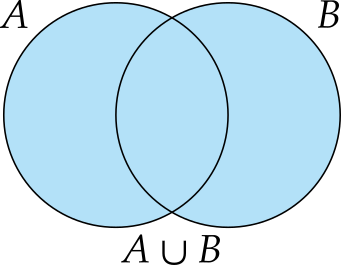
\includegraphics[width=6cm,height=\textheight]{img/teoria-conjuntos/union.png}

}

\caption{Unión de conjuntos}

\end{figure}

\begin{example}[]\protect\hypertarget{exm-union-conjuntos}{}\label{exm-union-conjuntos}

Dado el conjunto de los números que contiene un dado,
\(\Omega=\{1,2,3,4,5,6\}\) y sus subconjuntos \(A=\{2,4,6\}\) y
\(B=\{1,2,3,4\}\),la unión de \(A\) y \(B\) es
\(A\cup B=\{1,2,3,4,6\}\).

\end{example}

\begin{definition}[Intersección]\protect\hypertarget{def-interseccion-conjuntos}{}\label{def-interseccion-conjuntos}

Dados dos conjuntos \(A\) y \(B\), se llama \emph{intersección} de \(A\)
y \(B\), y se denota \(A\cap B\), al conjunto de todos los elementos
comunes a \(A\) y \(B\).

\[A\cap B = \{x\,:\, x\in A\mbox{ y }x\in B\}.\]

\end{definition}

\begin{figure}

{\centering 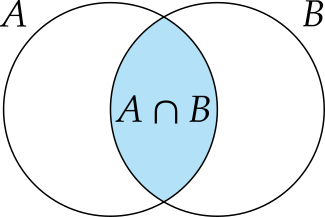
\includegraphics[width=6cm,height=\textheight]{img/teoria-conjuntos/interseccion.png}

}

\caption{Intersección de conjuntos}

\end{figure}

\begin{example}[]\protect\hypertarget{exm-interseccion-conjuntos}{}\label{exm-interseccion-conjuntos}

Dado el conjunto de los números que contiene un dado,
\(\Omega=\{1,2,3,4,5,6\}\) y sus subconjuntos \(A=\{2,4,6\}\) y
\(B=\{1,2,3,4\}\),la intersección de \(A\) y \(B\) es
\(A\cap B=\{2,4\}\).

\end{example}

\begin{definition}[Complemento]\protect\hypertarget{def-complemento-conjuntos}{}\label{def-complemento-conjuntos}

Dado un conjunto \(A\subset \Omega\), se llama \emph{complemento} de
\(A\) con respecto a \(\Omega\), y se denota \(\overline A\), al
conjunto de todos los elementos de \(\Omega\) que no pertenecen a \(A\).

\[\overline A = \{x\in \Omega\,:\, x\not\in A\}.\]

\end{definition}

\begin{figure}

{\centering 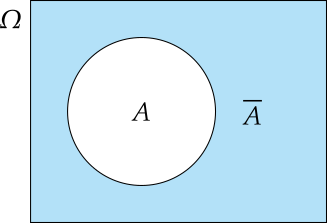
\includegraphics[width=7cm,height=\textheight]{img/teoria-conjuntos/complemento.png}

}

\caption{Complemento de un conjunto}

\end{figure}

\begin{example}[]\protect\hypertarget{exm-complemento-conjuntos}{}\label{exm-complemento-conjuntos}

Dado el conjunto de los números que contiene un dado,
\(\Omega=\{1,2,3,4,5,6\}\) y sus subconjuntos \(A=\{2,4,6\}\) y
\(B=\{1,2,3,4\}\), el contrario de \(A\) con respecto a \(\Omega\) es
\(\overline A=\{1,3,5\}\), y el de \(B\) es \(\overline B = \{5, 6\}\).

\end{example}

\begin{definition}[Diferencia]\protect\hypertarget{def-diferencia-conjuntos}{}\label{def-diferencia-conjuntos}

Dados dos conjuntos \(A\) y \(B\), se llama \emph{diferencia} de \(A\) y
\(B\), y se denota \(A-B\), al conjunto formado por los elementos de
\(A\) que no pertenecen a \(B\), es decir,

\[A-B = \{x\,:\, x\in A\mbox{ y }x\not\in B\}.\]

\end{definition}

\begin{figure}

{\centering 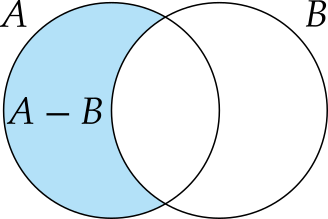
\includegraphics[width=6cm,height=\textheight]{img/teoria-conjuntos/diferencia.png}

}

\caption{Diferencia de conjuntos}

\end{figure}

\begin{example}[]\protect\hypertarget{exm-diferencia-conjuntos}{}\label{exm-diferencia-conjuntos}

Dado el conjunto de los números que contiene un dado,
\(\Omega=\{1,2,3,4,5,6\}\) y sus subconjuntos \(A=\{2,4,6\}\) y
\(B=\{1,2,3,4\}\),la diferencia de \(A\) y \(B\) es \(A-B=\{6\}\), y la
diferencia de \(B\) y \(A\) es \(B-A=\{1,3\}\).

\end{example}

\begin{definition}[Diferencia
simétrica]\protect\hypertarget{def-diferencia-simetrica-conjuntos}{}\label{def-diferencia-simetrica-conjuntos}

Dados dos conjuntos \(A\) y \(B\), se llama \emph{diferencia simétrica}
de \(A\) y \(B\), y se denota \(A\triangle B\), al conjunto formado por
los elementos que pertenecen a \(A\) o \(B\), pero no a ambos a la vez,
es decir,

\begin{align*}
A\triangle B &= \{x\,:\, x\in A-B\mbox{ o }x\in B-A\}\\ 
&= (A-B) \cup (B-A) = (A\cup B)-(A\cap B)
\end{align*}

\end{definition}

\begin{figure}

{\centering 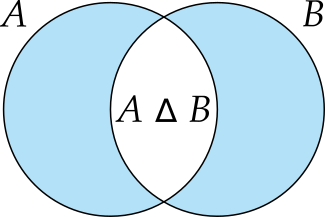
\includegraphics[width=6cm,height=\textheight]{img/teoria-conjuntos/diferencia-simetrica.png}

}

\caption{Diferencia simétrica de conjuntos}

\end{figure}

\begin{example}[]\protect\hypertarget{exm-diferencia-simetrica-conjuntos}{}\label{exm-diferencia-simetrica-conjuntos}

Dado el conjunto de los números que contiene un dado,
\(\Omega=\{1,2,3,4,5,6\}\) y sus subconjuntos \(A=\{2,4,6\}\) y
\(B=\{1,2,3,4\}\),la diferencia simétrica de \(A\) y \(B\) es
\(A\triangle B = \{1, 3, 6\}\).

\end{example}

\begin{proposition}[]\protect\hypertarget{prp-propiedades-conjuntos}{}\label{prp-propiedades-conjuntos}

Dado un conjunto universo \(\Omega\) y los conjuntos
\(A,B,C\subseteq \Omega\), se cumplen las siguientes propiedades:

\begin{enumerate}
\def\labelenumi{\arabic{enumi}.}
\tightlist
\item
  Idempotencia: \(A\cup A=A\) y \(A\cap A=A\).
\item
  Conmutativa: \(A\cup B=B\cup A\) y \(A\cap B = B\cap A\).
\item
  Asociativa: \((A\cup B)\cup C = A\cup (B\cup C)\) y
  \((A\cap B)\cap C = A\cap (B\cap C)\).
\item
  Distributiva: \((A\cup B)\cap C = (A\cap C)\cup (B\cap C)\) y
  \((A\cap B)\cup C = (A\cup C)\cap (B\cup C)\).
\item
  Elemento neutro: \(A\cup \emptyset=A\) y \(A\cap \Omega=A\).
\item
  Elemento absorvente: \(A\cup \Omega=\Omega\) y
  \(A\cap \emptyset=\emptyset\).
\item
  Elemento simétrico complementario: \(A\cup \overline A = E\) y
  \(A\cap \overline A= \emptyset\).
\item
  Doble complemento: \(\overline{\overline A} = A\).
\item
  Leyes de Morgan: \(\overline{A\cup B} = \overline A\cap \overline B\)
  y \(\overline{A\cap B} = \overline A\cup \overline B\).
\item
  \(A\cap B\subseteq A\cup B\).
\item
  \(A-B = A \cap \overline B\).
\item
  \(A-B\subseteq A\) y \(B-A\subseteq B\).
\item
  \(A\triangle B = (A\cup B) - (A\cap B)\).
\item
  \(\overline \Omega = \emptyset\) y \(\overline \emptyset = \Omega\).
\end{enumerate}

\end{proposition}

\begin{definition}[Conjuntos
disjuntos]\protect\hypertarget{def-conjuntos-disjuntos}{}\label{def-conjuntos-disjuntos}

Dados dos conjuntos \(A\) y \(B\), se dice que son \emph{disjuntos} si
no tienen ningún elemento en común, es decir, \(A\cap B=\emptyset\).

\end{definition}

\begin{example}[]\protect\hypertarget{exm-conjuntos-disjuntos}{}\label{exm-conjuntos-disjuntos}

Dado el conjunto de los números que contiene un dado,
\(\Omega=\{1,2,3,4,5,6\}\), y sus subconjuntos \(A=\{2,4,6\}\),
\(B=\{1,2,3,4\}\) y \(C=\{3, 5\}\), se tiene que \(A\) y \(B\) no son
disjuntos ya que \(A\cap B=\{2, 4\}\neq \emptyset\), pero \(A\) y \(C\)
son disjuntos pues \(A\cap C=\emptyset\).

\end{example}

\begin{definition}[Conjunto
potencia]\protect\hypertarget{def-conjunto-potencia}{}\label{def-conjunto-potencia}

Dado un conjunto \(A\), se llama \emph{conjunto potencia} o
\emph{conjunto de las partes} de \(A\), y se denota \(\mathcal{P}(A)\),
al conjunto de todos los subconjuntos de \(A\), es decir,

\[\mathcal{P}(A) = \{ X \, : \,  X \subseteq A \}\]

\end{definition}

\begin{example}[]\protect\hypertarget{exm-conjunto-potencia}{}\label{exm-conjunto-potencia}

El conjunto potencia del conjunto \(A=\{1, 2, 3\}\) es

\end{example}

\[\mathcal{P}(A)=\{\emptyset, \{1\}, \{2\}, \{3\}, \{1,2\}, \{1,3\}, \{2,3\}, \{1,2,3\}\}\]

\hypertarget{relaciones-entre-conjuntos}{%
\section{Relaciones entre conjuntos}\label{relaciones-entre-conjuntos}}

\begin{definition}[Par
ordenado]\protect\hypertarget{def-par-ordenado}{}\label{def-par-ordenado}

Dados dos elementos \(a\) y \(b\) se define el \emph{par ordenado}
\((a,b)\) como \[ (a,b) = \{\{a\}, \{a,b\}\} \]

De manera más general, se define una \emph{\(n\)-tupla ordenada} como
\[(a_1, a_2, \ldots, a_n) = ((a_1, a_2, \ldots, a_{n-1}), a_n)\]

\end{definition}

De forma mas informal, decimos que \((a,b)\) es un par ordenado si el
primer elemento (\(a\)) se distingue del segundo elemento (\(b\)). Por
eso, se tiene que \((a,b) \neq (b,a)\), mientras que para conjuntos
\(\{a,b\}=\{b,a\}\).

\begin{definition}[Producto
cartesiano]\protect\hypertarget{def-producto-cartesiano}{}\label{def-producto-cartesiano}

Dados dos conjuntos \(A\) y \(B\), se llama \emph{producto cartesiano}
de \(A\) y \(B\), y se denota \(A\times B\), al conjunto de los pares
ordenados

\[A \times B = \{ (a,b) \, : \,  a \in A \mbox{ y } b \in B \}\]

De manera más general, si se tienen \(n\) conjuntos
\(A_1, A_2, \ldots, A_n\), el \emph{producto cartesiano generalizado} es

\[A_1 \times A_2 \times \ldots \times A_n = \{ (a_1, \ldots, a_n) \, :\, a_i \in A_i\ \forall i=1, \ldots n\}\]

\end{definition}

\begin{example}[]\protect\hypertarget{exm-producto-cartesiano}{}\label{exm-producto-cartesiano}

El producto cartesiano de los conjuntos \(A=\{a, b, c\}\) y
\(B=\{1, 2\}\) es

\[
A\times B = \{(a,1), (a,2), (b,1), (b,2), (c,1), (c,2)\}
\]

\end{example}

\begin{definition}[Relación
binaria]\protect\hypertarget{def-relacion-binaria}{}\label{def-relacion-binaria}

Dados dos conjuntos \(A\) y \(B\), se dice que \(R\) es una
\emph{relación binaria} sobre \(A\) y \(B\) si es un subconjunto del
producto cartesiano de \(A\) y \(B\), es decir, \[ 
R \subseteq A \times B.
\]

Si \((a,b)\in R\) se escribe \(a R b\).

Si \(A\) y \(B\) son el mismo conjunto, se dice que \(R\) es una
\emph{relación binaria homogénea}.

\end{definition}

Cuando un par ordenado pertenece a una relación, \((a,b)\in R\), también
se suele escribir \(aRb\).

Dependiendo de las propiedades que cumpla una relación binaria homogénea
tenemos los siguientes tipos de relaciones:

\begin{itemize}
\tightlist
\item
  \textbf{Reflexiva}: \(\forall a \in A, (a,a) \in R\)
\item
  \textbf{Irreflexiva}: \(\forall a \in A, (a,a) \not\in R\).
\item
  \textbf{Simétrica}: \(\forall a, b \in A\), si \((a,b) \in R\),
  entonces \((b,a) \in R\).
\item
  \textbf{Asimétrica}: \(\forall a, b \in A\), si \((a,b) \in R\),
  entonces \((b,a) \not\in R\).
\item
  \textbf{Antisimétrica}: \(\forall a, b \in A\), si \((a,b) \in R\) y
  \((b,a) \in R\), entonces \(a = b\).
\item
  \textbf{Transitiva}: \(\forall a, b, c \in A\), si \((a,b) \in R\) y
  \((b,c) \in R\), entonces \((a,c) \in R\).
\item
  \textbf{Total}: \(\forall a, b \in A\), \((a,b) \in R\) o
  \((b,a) \in R\).
\end{itemize}

\begin{definition}[Relación de
equivalencia]\protect\hypertarget{def-relacion-equivalencia}{}\label{def-relacion-equivalencia}

Dado un conjunto \(A\) y una relación homogénea
\(\sim \subseteq A \times A\), se dice que \(\sim\) es una
\emph{relación de equivalencia} si es que cumple que \(\sim\) es
reflexiva, simétrica y transitiva, es decir, si cumple las propiedades

\begin{itemize}
\tightlist
\item
  \emph{Reflexiva:} \(\forall a \in A, a \sim a\).
\item
  \emph{Simétrica:} \(\forall a, b \in A\), si \(a\sim b\) entonces
  \(b\sim a\).
\item
  \emph{Transitiva:} \(\forall a, b, c \in A\), si \(a\sim b\) y
  \(b\sim c\), entonces \(a\sim c\).
\end{itemize}

\end{definition}

\begin{example}[]\protect\hypertarget{exm-relacion-equivalencia}{}\label{exm-relacion-equivalencia}

Ya hemos visto que la relación de igualdad matemática entre los
elementos de un conjunto es una relación de equivalencia.

\end{example}

\begin{definition}[Relación de
orden]\protect\hypertarget{def-relacion-orden}{}\label{def-relacion-orden}

Dado un conjunto \(A\) y una relación homogénea
\(\preceq \subseteq A \times A\), se dice que \(\preceq\) es una
\emph{relación de orden}, si es una relación reflexiva, antisimétrica y
transitiva, es decir, si cumple las propiedades

\begin{itemize}
\tightlist
\item
  \emph{Reflexiva:} \(\forall a \in A, a \preceq a\).
\item
  \emph{Antisimétrica:} \(\forall a, b \in A\), si \(a\preceq b\) y
  \(b\preceq a\), entonces \(a = b\).
\item
  \emph{Transitiva:} \(\forall a, b, c \in A\), si \(a\preceq b\) y
  \(b\preceq c\), entonces \(a\preceq c\).
\end{itemize}

\end{definition}

\begin{definition}[Relación de orden
parcial]\protect\hypertarget{def-relacion-orden-parcial}{}\label{def-relacion-orden-parcial}

Dado un conjunto \(A\) y una relación homogénea
\(\preceq \subseteq A \times A\), se dice que \(\preceq\) es una
\emph{relación de orden parcial}, si es una relación de orden y al menos
dos elementos de \(A\) están relacionados mediante \(\preceq\), es
decir,

\[\exists x, y\in A,\ x\preceq y \mbox{ o } y\preceq x.\]

Al conjunto \(A\) con la relación de orden parcial \(\preceq\) se le
llama \emph{conjunto parcialmente ordenado}, y se denota
\((A,\preceq)\).

\end{definition}

\begin{example}[]\protect\hypertarget{exm-relacion-orden-parcial}{}\label{exm-relacion-orden-parcial}

El conjunto potencia de un conjunto \(A\) con la relación de inclusión
es un conjunto parcialmente ordenado \((\mathcal{P}(A),\subseteq)\).

\end{example}

\begin{definition}[Relación de orden
total]\protect\hypertarget{def-relacion-orden-total}{}\label{def-relacion-orden-total}

Dado un conjunto \(A\) y una relación homogénea
\(\preceq \subseteq A \times A\), se dice que \(\preceq\) es una
\emph{relación de orden total}, si es una relación de orden y todos los
elementos de \(A\) se relacionan entre sí mediante \(\preceq\), es
decir,

\[\forall x, y\in A,\ x\preceq y \mbox{ o } y \preceq x.\]

Al conjunto \(A\) con la relación de orden total \(\preceq\) se le llama
\emph{conjunto totalmente ordenado}, y se denota \((A,\preceq)\).

\end{definition}

\begin{example}[]\protect\hypertarget{exm-relacion-orden-total}{}\label{exm-relacion-orden-total}

La relación de orden de los números naturales \((\mathbb{N},\leq)\) es
un orden totalmente ordenado. Sin embargo, la relación de inclusión en
el conjunto potencia de un conjunto \(A\) (\(\mathcal{P}(A),\subseteq\))
no es un orden totalmente ordenado, ya que dados dos elementos
\(a\neq b\) de \(A\), se cumple que \(\{a\}\subsetneq \{b\}\) y
\(\{b\}\subsetneq \{a\}\).

\end{example}

\hypertarget{cotas-y-extremos}{%
\section{Cotas y extremos}\label{cotas-y-extremos}}

\begin{definition}[Cota
superior]\protect\hypertarget{def-cota-superior-conjunto}{}\label{def-cota-superior-conjunto}

Dado un subconjunto con una relación de orden parcial \((A,\preceq)\) y
un subconjunto \(B\subseteq A\), se dice que un elemento \(c\in A\) es
una \emph{cota superior} de \(B\), si todos los elementos de \(B\) son
menores o iguales a \(c\) según la relación de orden, es decir,

\[\forall x \in B, x\preceq c.\]

El conjunto de todas las cotas superiores de \(B\) se denota
\(\operatorname{CS}(B)\).

\end{definition}

\begin{example}[]\protect\hypertarget{exm-cota-superior}{}\label{exm-cota-superior}

Para el conjunto \(B=\{3, 4, 5\}\subseteq \mathbb{N}\), \(5\) es una
cota superior. El conjunto de todas sus cotas superiores es
\(\operatorname{CS}(B)=\{x\in \mathbb{N}:x\geq 5\}\).

Para el intervalo \([0,1)\subseteq \mathbb{R}\), cualquier número real
\(x\geq 1\) es una cota superior, por lo que
\(\operatorname{CS}([0,1)) = \{x\in \mathbb{R}:x\geq 1\}\).

\end{example}

\begin{definition}[Cota
inferior]\protect\hypertarget{def-cota-inferior-conjunto}{}\label{def-cota-inferior-conjunto}

Dado un subconjunto con una relación de orden parcial \((A,\preceq)\) y
un subconjunto \(B\subseteq A\), se dice que un elemento \(c\in A\) es
una \emph{cota inferior} de \(B\), si todos los elementos de \(B\) son
mayores o iguales a \(c\) según la relación de orden, es decir,

\[\forall x \in B, c\preceq x.\]

El conjunto de todas las cotas inferiores de \(B\) se denota
\(\operatorname{CI}(B)\).

\end{definition}

\begin{example}[]\protect\hypertarget{exm-cota-inferior}{}\label{exm-cota-inferior}

El conjunto de las cotas inferiores de
\(B=\{3, 4, 5\}\subseteq \mathbb{N}\) es
\(\operatorname{CI}(B)=\{1, 2, 3\}\).

El conjunto de las cotas inferiores de \([0,1)\subseteq \mathbb{R}\) es
\(\operatorname{CI}([0,1)) = \{x\in \mathbb{R}:x\leq 0\}\).

\end{example}

\begin{definition}[Máximo]\protect\hypertarget{def-maximo-conjunto}{}\label{def-maximo-conjunto}

Dado un conjunto con una relación de orden parcial \((A,\preceq)\), se
dice que un elemento \(m\in A\) es un \emph{máximo} de \(A\), y se
denota \(\max(A)\), si cualquier otro elemento de \(A\) es menor o igual
que él según la relación de orden, es decir,

\[\forall x \in A, x\preceq m.\]

\end{definition}

\begin{example}[]\protect\hypertarget{exm-maximo}{}\label{exm-maximo}

El máximo de \(B=\{3, 4, 5\}\subseteq \mathbb{N}\), es \(5\).

El intervalo \([0,1)\subseteq \mathbb{R}\) no tiene máximo.

\end{example}

\begin{definition}[Mínimo]\protect\hypertarget{def-minimo-conjunto}{}\label{def-minimo-conjunto}

Dado un conjunto con una relación de orden parcial \((A,\preceq)\), se
dice que un elemento \(m\in A\) es un \emph{mínimo} de \(A\), y se
denota \(\min(A)\), si y cualquier otro elemento de \(A\) es mayor o
igual que él según la relación de orden, es decir,

\[\forall x \in A, m\preceq x.\]

\end{definition}

\begin{example}[]\protect\hypertarget{exm-maximo}{}\label{exm-maximo}

El mínimo de \(B=\{3, 4, 5\}\subseteq \mathbb{N}\), es \(3\).

El mínimo del intervalo \([0,1)\subseteq \mathbb{R}\) es \(0\).

\end{example}

\begin{theorem}[Unicidad de los
extremos]\protect\hypertarget{thm-unicidad-extremos}{}\label{thm-unicidad-extremos}

Dado un conjunto con una relación de orden parcial \((A,\preceq)\), si
existe el máximo de \(A\) entonces es único. Lo mismo es cierto para el
mínimo.

\end{theorem}

\begin{tcolorbox}[enhanced jigsaw, colback=white, colbacktitle=quarto-callout-note-color!10!white, title=\textcolor{quarto-callout-note-color}{\faInfo}\hspace{0.5em}{Demostración}, rightrule=.15mm, coltitle=black, arc=.35mm, opacityback=0, colframe=quarto-callout-note-color-frame, bottomtitle=1mm, titlerule=0mm, toptitle=1mm, bottomrule=.15mm, toprule=.15mm, breakable, opacitybacktitle=0.6, left=2mm, leftrule=.75mm]

\begin{proof}

Supongamos que \(A\) tiene dos máximos \(m\) y \(n\). Entonces, por la
definición de máximo, \(x\preceq m\) \(\forall x\in A\), y en particular
\(n\preceq m\). Del mismo modo, \(x\preceq n\) \(\forall x\in A\), y en
particular \(m\preceq n\), pero como \(\preceq\) es una relación de
orden, se deduce que \(m=n\).

\end{proof}

\end{tcolorbox}

\begin{definition}[Supremo]\protect\hypertarget{def-supremo-conjunto}{}\label{def-supremo-conjunto}

Dado un subconjunto con una relación de orden parcial \((A,\preceq)\) y
un subconjunto \(B\subseteq A\), se llama \emph{supremo} de \(B\), y se
denota \(\sup(B)\), a la menor de las cotas superiores de \(B\).

\end{definition}

\begin{example}[]\protect\hypertarget{exm-supremo}{}\label{exm-supremo}

El supremo del conjunto \(B=\{3, 4, 5\}\subseteq \mathbb{N}\), es \(5\)
ya que es el mínimo del conjunto de sus cotas superiores
\(\operatorname{CS}(B)=\{x\in \mathbb{N}:x\geq 5\}\).

El supremo del intervalo \([0,1)\subseteq \mathbb{R}\) es \(1\) ya que
es el mínimo del conjunto de sus cotas superiores
\(\operatorname{CS}([0,1)) = \{x\in \mathbb{R}:x\geq 1\}\).

\end{example}

\begin{definition}[Ínfimo]\protect\hypertarget{def-infimo-conjunto}{}\label{def-infimo-conjunto}

Dado un subconjunto con una relación de orden parcial \((A,\preceq)\) y
un subconjunto \(B\subseteq A\), se llama \emph{ínfimo} de \(B\), y se
denota \(\inf(B)\), a la mayor de las cotas inferiores de \(B\).

\end{definition}

\begin{example}[]\protect\hypertarget{exm-infimo}{}\label{exm-infimo}

El ínfimo del conjunto \(B=\{3, 4, 5\}\subseteq \mathbb{N}\), es \(3\)
ya que es el máximo del conjunto de sus cotas inferiores
\(\operatorname{CI}(B)=\{1, 2, 3\}\).

El ínfimo del intervalo \([0,1)\subseteq \mathbb{R}\) es \(0\) ya que es
el máximo del conjunto de sus cotas inferiores
\(\operatorname{CI}([0,1)) = \{x\in \mathbb{R}:x\leq 0\}\).

\end{example}

\begin{tcolorbox}[enhanced jigsaw, colback=white, colbacktitle=quarto-callout-warning-color!10!white, title=\textcolor{quarto-callout-warning-color}{\faExclamationTriangle}\hspace{0.5em}{Advertencia}, rightrule=.15mm, coltitle=black, arc=.35mm, opacityback=0, colframe=quarto-callout-warning-color-frame, bottomtitle=1mm, titlerule=0mm, toptitle=1mm, bottomrule=.15mm, toprule=.15mm, breakable, opacitybacktitle=0.6, left=2mm, leftrule=.75mm]

Obsérvese que un conjunto puede no tener cotas superiores o inferiores
y, por tanto, no tener supremo o ínfimo.

\end{tcolorbox}

\begin{example}[]\protect\hypertarget{exm-no-supremo-infimio}{}\label{exm-no-supremo-infimio}

El conjunto \(B=\{x\in\mathbb{Z}: x \mbox{ es par}\}\), no tiene cotas
superiores, ni inferiores, y por tanto tampoco tiene máximo, mínimo,
supremo e ínfimo.

\end{example}

\hypertarget{funciones}{%
\section{Funciones}\label{funciones}}

El concepto de función es uno de los más importantes en el Análisis
Matemático, ya que muchos de los fenómenos naturales en los que una
magnitud depende de otra se modelizan mediante funciones.

\begin{definition}[Función]\protect\hypertarget{def-funcion}{}\label{def-funcion}

Se dice que una relación binaria \(f \subseteq A \times B\), con \(A\) y
\(B\) conjuntos no vacíos, es una \emph{función parcial} o
\emph{aplicación parcial}, y se denota \(f:A\rightarrow B\), si \(f\) no
contiene dos pares ordenados distintos con la misma primera componente,
es decir,

\[
\forall a \in A, \forall b_1, b_2 \in B, \mbox{ si } (a,b_1) \in f \mbox{ y } (a,b_2) \in f, \mbox{ entonces } b_1 = b_2.
\]

Si además, la relación es total en \(A\), es decir, todos los elementos
de \(A\) aparecen en la relación, se dice que \(f\) es una \emph{función
total} o simplemente \emph{función}.

\end{definition}

De manera más informal podemos decir que una función es una
correspondencia entre los elementos de dos conjuntos \(A\) y \(B\) que
asocia a cada elemento de \(A\) un elemento, y solo uno, de \(B\).

Es habitual representar los pares de una función con la notación
\(y=f(x)\) donde \(x\) es la primera componente del par e \(y\) la
segunda.

\begin{example}[]\protect\hypertarget{exm-funcion}{}\label{exm-funcion}

La relación binaria \(f=\{(1,d), (2,c), (3,a), (4,c)\}\) es una función,
pero la relación \(g=\{(1,d), (2,b), (3,a), (3,c)\}\) no lo es porque
existen dos pares cuya primera componente es \(3\).

Del mismo modo la función raíz cuadrada \(y=f(x)=\sqrt{x}\) no es una
función en el conjunto de los números reales, ya que, por ejemplo
\(\sqrt{1}=\pm 1\).

\end{example}

\begin{figure}

\begin{minipage}[t]{0.50\linewidth}

{\centering 

\raisebox{-\height}{

\begin{tikzpicture}[scale=1.5,every node/.style={transform shape}]
\filldraw[fill=blue!20, draw=blue!60] (-1.5,0) ellipse (1cm and 1.5cm);
\filldraw[fill=red!20, draw=red!60] (1.5,0) ellipse (1cm and 1.5cm);

    \node at (-1.5,1.8) {$A$};
    \node at (1.5,1.8) {$B$};

    \node (x1) at (-1.5,0.9) {$1$};
    \node (x2) at (-1.5,0.3) {$2$};
    \node (x3) at (-1.5,-0.3) {$3$};
    \node (x4) at (-1.5,-0.9) {$4$};
    \node (y1) at (1.5,0.9) {$a$};
    \node (y2) at (1.5,0.3) {$b$};
    \node (y3) at (1.5,-0.3) {$c$};
    \node (y4) at (1.5,-0.9) {$d$};

    % draw the arrows
    \draw[-stealth] (x1) -- (y4);
    \draw[-stealth] (x2) -- (y3);
    \draw[-stealth] (x3) -- (y1);
    \draw[-stealth] (x4) -- (y3);

\end{tikzpicture}

}

\caption{Ejemplo de función}

}

\end{minipage}%
%
\begin{minipage}[t]{0.50\linewidth}

{\centering 

\raisebox{-\height}{

\begin{tikzpicture}[scale=1,every node/.style={transform shape}]
\filldraw[fill=blue!20, draw=blue!60] (-1.5,0) ellipse (1cm and 1.5cm);
\filldraw[fill=red!20, draw=red!60] (1.5,0) ellipse (1cm and 1.5cm);

    \node at (-1.5,1.8) {$A$};
    \node at (1.5,1.8) {$B$};

    \node (x1) at (-1.5,0.6) {$1$};
    \node (x2) at (-1.5,0.0) {$2$};
    \node (x3) at (-1.5,-0.6) {$3$};
   % \node (x4) at (-1.5,-0.9) {$4$};
    \node (y1) at (1.5,0.9) {$a$};
    \node (y2) at (1.5,0.3) {$b$};
    \node (y3) at (1.5,-0.3) {$c$};
    \node (y4) at (1.5,-0.9) {$d$};

    % draw the arrows
    \draw[-stealth] (x1) -- (y4);
    \draw[-stealth] (x2) -- (y2);
    \draw[-stealth] (x3) -- (y1);
    \draw[-stealth] (x3) -- (y3);
    %\draw[-stealth] (x4) -- (y3);

\end{tikzpicture}

}

\caption{Ejemplo de no función}

}

\end{minipage}%

\end{figure}

\begin{definition}[Dominio]\protect\hypertarget{def-dominio-funcion}{}\label{def-dominio-funcion}

Dada una función \(f:A\rightarrow B\), se llama \emph{dominio} de \(f\),
y se denota \(\operatorname{Dom}(f)\) al conjunto de las primeras
componentes de los pares de \(f\), es decir,

\[\operatorname{Dom}(f) = \{a\in A: \exists b\in B, (a,b)\in f\}\]

\end{definition}

\begin{definition}[Imagen]\protect\hypertarget{def-imagen-funcion}{}\label{def-imagen-funcion}

Dada una función \(f:A\rightarrow B\), se llama \emph{imagen} de \(f\),
y se denota \(\operatorname{Im}(f)\) al conjunto de las segundas
componentes de los pares de \(f\), es decir,

\[\operatorname{Im}(f) = \{b\in B: \exists a\in A, (a,b)\in f\}\]

\end{definition}

\begin{definition}[Función
inyectiva]\protect\hypertarget{def-funcion-inyectiva}{}\label{def-funcion-inyectiva}

Dada una función \(f:A\rightarrow B\), se dice que \(f\) es
\emph{inyectiva} si no existen dos elementos de \(A\) con la misma
imagen, es decir,

\[\forall a_1, a_2 \in A, \mbox{ si } f(a_1) = f(a_2), \mbox{ entonces } a_1 = a_2.\]

\end{definition}

\begin{definition}[Función
sobreyectiva]\protect\hypertarget{def-funcion-sobreyectiva}{}\label{def-funcion-sobreyectiva}

Dada una función \(f:A\rightarrow B\), se dice que \(f\) es
\emph{sobreyectiva} si todo elemento de \(B\) tiene una preimagen (está
relacionado con algún elemento de \(A\) mediante \(f\)), es decir,

\[\forall b \in B, \exists a\in A, f(a) = b.\]

\end{definition}

\begin{definition}[Función
biyectiva]\protect\hypertarget{def-funcion-biyectiva}{}\label{def-funcion-biyectiva}

Dada una función \(f:A\rightarrow B\), se dice que \(f\) es
\emph{biyectiva}, si \(f\) es, a la vez, inyectiva y sobreyectiva.

\end{definition}

\begin{figure}

\begin{minipage}[t]{0.50\linewidth}

{\centering 

\raisebox{-\height}{

\begin{tikzpicture}[scale=1.5,every node/.style={transform shape}]
\filldraw[fill=blue!20, draw=blue!60] (-1.5,0) ellipse (1cm and 1.5cm);
\filldraw[fill=red!20, draw=red!60] (1.5,0) ellipse (1cm and 1.5cm);

    \node at (-1.5,1.8) {$A$};
    \node at (1.5,1.8) {$B$};

    \node (x1) at (-1.5,0.6) {$1$};
    \node (x2) at (-1.5,0) {$2$};
    \node (x3) at (-1.5,-0.6) {$3$};
%    \node (x4) at (-1.5,-0.9) {$4$};
    \node (y1) at (1.5,0.9) {$a$};
    \node (y2) at (1.5,0.3) {$b$};
    \node (y3) at (1.5,-0.3) {$c$};
    \node (y4) at (1.5,-0.9) {$d$};

    % draw the arrows
    \draw[-stealth] (x1) -- (y4);
    \draw[-stealth] (x2) -- (y2);
    \draw[-stealth] (x3) -- (y1);
    %\draw[-stealth] (x4) -- (y3);

\end{tikzpicture}

}

\caption{Función inyectiva y no sobreyectiva}

}

\end{minipage}%
%
\begin{minipage}[t]{0.50\linewidth}

{\centering 

\raisebox{-\height}{

\begin{tikzpicture}[scale=1,every node/.style={transform shape}]
\filldraw[fill=blue!20, draw=blue!60] (-1.5,0) ellipse (1cm and 1.5cm);
\filldraw[fill=red!20, draw=red!60] (1.5,0) ellipse (1cm and 1.5cm);

    \node at (-1.5,1.8) {$A$};
    \node at (1.5,1.8) {$B$};

    \node (x1) at (-1.5,0.9) {$1$};
    \node (x2) at (-1.5,0.3) {$2$};
    \node (x3) at (-1.5,-0.3) {$3$};
    \node (x4) at (-1.5,-0.9) {$4$};
    \node (y1) at (1.5,0.6) {$a$};
    \node (y2) at (1.5,0) {$b$};
    \node (y3) at (1.5,-0.6) {$c$};
    %\node (y4) at (1.5,-0.9) {$d$};

    % draw the arrows
    \draw[-stealth] (x2) -- (y3);
    \draw[-stealth] (x1) -- (y2);
    \draw[-stealth] (x3) -- (y1);
    \draw[-stealth] (x4) -- (y3);

\end{tikzpicture}

}

\caption{Función sobreyectiva y no inyectiva}

}

\end{minipage}%
\newline
\begin{minipage}[t]{0.50\linewidth}

{\centering 

\raisebox{-\height}{

\begin{tikzpicture}[scale=1.5,every node/.style={transform shape}]
\filldraw[fill=blue!20, draw=blue!60] (-1.5,0) ellipse (1cm and 1.5cm);
\filldraw[fill=red!20, draw=red!60] (1.5,0) ellipse (1cm and 1.5cm);

    \node at (-1.5,1.8) {$A$};
    \node at (1.5,1.8) {$B$};

    \node (x1) at (-1.5,0.9) {$1$};
    \node (x2) at (-1.5,0.3) {$2$};
    \node (x3) at (-1.5,-0.3) {$3$};
    \node (x4) at (-1.5,-0.9) {$4$};
    \node (y1) at (1.5,0.9) {$a$};
    \node (y2) at (1.5,0.3) {$b$};
    \node (y3) at (1.5,-0.3) {$c$};
    \node (y4) at (1.5,-0.9) {$d$};

    % draw the arrows
    \draw[-stealth] (x1) -- (y4);
    \draw[-stealth] (x2) -- (y2);
    \draw[-stealth] (x3) -- (y1);
    \draw[-stealth] (x4) -- (y3);

\end{tikzpicture}

}

\caption{Función biyectiva}

}

\end{minipage}%
%
\begin{minipage}[t]{0.50\linewidth}

{\centering 

\raisebox{-\height}{

\begin{tikzpicture}[scale=1.5,every node/.style={transform shape}]
\filldraw[fill=blue!20, draw=blue!60] (-1.5,0) ellipse (1cm and 1.5cm);
\filldraw[fill=red!20, draw=red!60] (1.5,0) ellipse (1cm and 1.5cm);

    \node at (-1.5,1.8) {$A$};
    \node at (1.5,1.8) {$B$};

    \node (x1) at (-1.5,0.9) {$1$};
    \node (x2) at (-1.5,0.3) {$2$};
    \node (x3) at (-1.5,-0.3) {$3$};
    \node (x4) at (-1.5,-0.9) {$4$};
    \node (y1) at (1.5,0.9) {$a$};
    \node (y2) at (1.5,0.3) {$b$};
    \node (y3) at (1.5,-0.3) {$c$};
    \node (y4) at (1.5,-0.9) {$d$};

    % draw the arrows
    \draw[-stealth] (x1) -- (y4);
    \draw[-stealth] (x2) -- (y3);
    \draw[-stealth] (x3) -- (y1);
    \draw[-stealth] (x4) -- (y3);

\end{tikzpicture}

}

\caption{Función no inyectiva y no sobreyectiva}

}

\end{minipage}%

\end{figure}

\begin{definition}[Función
identidad]\protect\hypertarget{def-funcion-identidad}{}\label{def-funcion-identidad}

Dado un conjunto \(A\), se llama \emph{función identidad} de \(A\), y se
denota \(\operatorname{id}_A:A\rightarrow A\), a la función que empareja
cada elemento de \(A\) consigo mismo, es decir,

\[\operatorname{id}_A (a) = a, \forall a\in A.\]

\end{definition}

\begin{definition}[Función
inversa]\protect\hypertarget{def-funcion-inversa}{}\label{def-funcion-inversa}

Dada una función \(f:A\rightarrow B\), se llama \emph{función inversa}
de \(f\), y se denota \(f^{-1}:B\rightarrow A\), a la función que
resulta de revertir el orden de los pares de \(f\), es decir,

\[f^{-1} = \{ (b,a) : (a,b) \in f \}.\]

\end{definition}

Obsérvese que para que exista la función inversa de \(f\), \(f\) debe
ser inyectiva.

En muchas ocasiones, el valor de salida de una función se puede utilizar
como la entrada de otra función, concatenando la aplicación de las dos
funciones.

\begin{definition}[Composición de
funciones]\protect\hypertarget{def-composicion-funciones}{}\label{def-composicion-funciones}

Dadas dos funciones \(f:A\rightarrow B\) y \(g:C\rightarrow D\), tales
que \(\operatorname{Im}(f)\subseteq \operatorname{Dom}(g)\), se llama
\emph{composición} de \(f\) con \(g\), y se denota
\(g\circ f:A\rightarrow D\), a la funcion que a cada elemento del
dominio de \(A\) le asocia el elemento que resulta de aplicar \(g\) a la
imagen de \(a\) mediante \(f\), es decir,

\[g\circ f(a) = g(f(a)), \forall a\in A.\]

\end{definition}

\begin{proposition}[]\protect\hypertarget{prp-composicion-inversa}{}\label{prp-composicion-inversa}

Dada una función \(f:A\rightarrow B\), si existe \(f^{-1}\), entonces
\(f\circ f^{-1} = \operatorname{id}_A\) y
\(f^{-1}\circ f = \operatorname{id}_B\).

\end{proposition}

\begin{tcolorbox}[enhanced jigsaw, colback=white, colbacktitle=quarto-callout-note-color!10!white, title=\textcolor{quarto-callout-note-color}{\faInfo}\hspace{0.5em}{Demostración}, rightrule=.15mm, coltitle=black, arc=.35mm, opacityback=0, colframe=quarto-callout-note-color-frame, bottomtitle=1mm, titlerule=0mm, toptitle=1mm, bottomrule=.15mm, toprule=.15mm, breakable, opacitybacktitle=0.6, left=2mm, leftrule=.75mm]

\begin{proof}

Sea \(a\in\operatorname{Dom}(A)\), y supongamos que \(f(a)=b\). Entonces
\(f^{-1}(b)=a\), de manera que

\[
f\circ f^{-1}(a) 
= f(f^{-1}(a)) 
= f(b)
= a.
\]

\end{proof}

\end{tcolorbox}

\hypertarget{cardinalidad-de-un-conjunto}{%
\section{Cardinalidad de un
conjunto}\label{cardinalidad-de-un-conjunto}}

\begin{definition}[Cardinal]\protect\hypertarget{def-cardinal-conjunto}{}\label{def-cardinal-conjunto}

Dado un conjunto \(A\), se llama \emph{cardinal} de \(A\), y se denota
\(|A|\), al número de elementos de \(A\).

\end{definition}

De manera informal, se puede decir que el cardinal de un conjunto es su
tamaño.

\begin{example}[]\protect\hypertarget{exm-cardinal}{}\label{exm-cardinal}

El cardinal del conjunto \(A=\{a, b, c\}\) es \(|A|=3\).

\end{example}

\begin{proposition}[]\protect\hypertarget{prp-cardinal-conjunto-potencia}{}\label{prp-cardinal-conjunto-potencia}

El cardinal del conjunto potencia de un conjunto \(A\) es
\(|\mathcal{P}(A)| = 2^{|A|}\).

\end{proposition}

\begin{tcolorbox}[enhanced jigsaw, colback=white, colbacktitle=quarto-callout-note-color!10!white, title=\textcolor{quarto-callout-note-color}{\faInfo}\hspace{0.5em}{Demostración}, rightrule=.15mm, coltitle=black, arc=.35mm, opacityback=0, colframe=quarto-callout-note-color-frame, bottomtitle=1mm, titlerule=0mm, toptitle=1mm, bottomrule=.15mm, toprule=.15mm, breakable, opacitybacktitle=0.6, left=2mm, leftrule=.75mm]

\begin{proof}

Se puede dar una prueba mediante coeficientes binomiales. Si \(A\) tiene
\(n\) elementos, es decir, \(|\)A\(|=n\), el número de subconjuntos
distintos con \(k\) elementos es igual al número combinatorio
\[\binom{n}{k}=\frac{n!}{k!(n-k)!}.\]

Como un subconjunto de \(A\) puede tener desde \(0\) hasta \(n\)
elementos, en total, el número de posibles subconjuntos de \(A\) será

\[|\mathcal{P}(A)|=\binom{n}{0}+\binom{n}{1}+\cdots + \binom{n}{n} = \sum_{k=0}^n \binom{n}{k},\]

y según el teorema del binomio de Newton se tiene que

\[\sum_{k=0}^n \binom{n}{k}=2^n = 2^{|A|}.\]

\end{proof}

\end{tcolorbox}

\begin{definition}[Conjuntos
equipotentes]\protect\hypertarget{def-conjuntos-equipotentes}{}\label{def-conjuntos-equipotentes}

Se dice que dos conjuntos \(A\) y \(B\) son \emph{equipotentes}, y se
denota \(A\approx B\), si tienen la misma cantidad de elementos, es
decir, si \(|A| = |B|\).

\end{definition}

\begin{proposition}[]\protect\hypertarget{prp-biyeccion-conjuntos-equipotentes}{}\label{prp-biyeccion-conjuntos-equipotentes}

Dos conjuntos \(A\) y \(B\) son equipotentes si y solo si cada elemento
de \(A\) puede emparejarse con uno de \(B\), de manera que todos los
elementos de \(B\) sean pareja de uno de \(A\) y solo de uno, es decir,
existe una aplicación biyectiva \(f:A\rightarrow B\).

\end{proposition}

\begin{tcolorbox}[enhanced jigsaw, colback=white, colbacktitle=quarto-callout-note-color!10!white, title=\textcolor{quarto-callout-note-color}{\faInfo}\hspace{0.5em}{Demostración}, rightrule=.15mm, coltitle=black, arc=.35mm, opacityback=0, colframe=quarto-callout-note-color-frame, bottomtitle=1mm, titlerule=0mm, toptitle=1mm, bottomrule=.15mm, toprule=.15mm, breakable, opacitybacktitle=0.6, left=2mm, leftrule=.75mm]

\begin{proof}

Si \(A\) y \(B\) son equipotentes, es trivial construir una biyección
entre ellos, ya que podemos construir una función que empareje cada
elemento de \(A\) con un único elemento de \(B\) y cada elemento de
\(B\) con un único elemento de \(A\).

Por otro lado, si existe una aplicación biyectiva \(f\) entre \(A\) y
\(B\), la asociación entre elementos es uno a uno, es decir, para cada
elemento de \(A\) está emparejado exactamente con un uno de \(B\), y
cada elemento de \(B\) está emparejado exactamente con uno de \(A\), con
lo que necesariamente \(A\) y \(B\) deben tener el mismo número de
elementos.

\end{proof}

\end{tcolorbox}

\begin{proposition}[]\protect\hypertarget{prp-equipotencia-relacion-equivalencia}{}\label{prp-equipotencia-relacion-equivalencia}

La relación de equipotencia es una relación de equivalencia, es decir,
satisface las siguientes propiedades:

\begin{itemize}
\tightlist
\item
  \emph{Reflexiva:} \(A\approx A\) para todo conjunto \(A\).
\item
  \emph{Simétrica:} Si \(A\approx B\), entonces \(B\approx A\), para
  cualesquiera conjuntos \(A\) y \(B\).
\item
  \emph{Transitiva:} Si \(A\approx B\) y \(B\approx C\), entonces
  \(A\approx C\) para cualesquiera conjuntos \(A\), \(B\) y \(C\).
\end{itemize}

\end{proposition}

\begin{tcolorbox}[enhanced jigsaw, colback=white, colbacktitle=quarto-callout-note-color!10!white, title=\textcolor{quarto-callout-note-color}{\faInfo}\hspace{0.5em}{Demostración}, rightrule=.15mm, coltitle=black, arc=.35mm, opacityback=0, colframe=quarto-callout-note-color-frame, bottomtitle=1mm, titlerule=0mm, toptitle=1mm, bottomrule=.15mm, toprule=.15mm, breakable, opacitybacktitle=0.6, left=2mm, leftrule=.75mm]

\begin{proof}

Veamos que la relación de equipotencia cumple las propiedades reflexiva,
simétrica y transitiva.

Reflexiva: Es trivial ya que cualquier conjunto tiene el mismo número de
elementos que él mismo, luego \(A\approx A\).

Simétrica: Si \(A\approx B\) entonces, por la proposición anterior,
existe una una biyección \(f:A\longrightarrow B\). Pero entonces, la
función inversa \(f^{-1}:B\longrightarrow A\) es también una biyección
entre \(B\) y \(A\), por lo que \(B\approx A\).

Transitiva: Si \(A\approx B\) y \(B\approx C\), entonces, por la
proposición anterior, existen dos biyecciones \(f:A\longrightarrow B\) y
\(g:B\longrightarrow C\). Pero entonces, la función
\(g\circ f:A\longrightarrow C\) es también biyectiva, por lo que
\(A\approx C\).

\end{proof}

\end{tcolorbox}

De igual modo se puede definir una relación que capture la noción de que
un conjunto es de menor tamaño que otro.

\begin{definition}[Conjunto
minuspotente]\protect\hypertarget{def-conjuntos-minuspotentes}{}\label{def-conjuntos-minuspotentes}

Dados dos conjuntos \(A\) y \(B\), se dice que \(A\) es
\emph{minuspotente} a \(B\), y se denota \(A\preceq B\), si el cardinal
de \(A\) es menor o igual que el de \(B\), es decir, si
\(|A| \leq |B|\).

\end{definition}

\begin{proposition}[]\protect\hypertarget{prp-inyeccion-conjuntos-minuspotentes}{}\label{prp-inyeccion-conjuntos-minuspotentes}

El conjunto \(A\) es minuspotente al conjunto \(B\) si y solo si existe
una aplicación inyectiva \(f:A\rightarrow B\).

\end{proposition}

\begin{tcolorbox}[enhanced jigsaw, colback=white, colbacktitle=quarto-callout-note-color!10!white, title=\textcolor{quarto-callout-note-color}{\faInfo}\hspace{0.5em}{Demostración}, rightrule=.15mm, coltitle=black, arc=.35mm, opacityback=0, colframe=quarto-callout-note-color-frame, bottomtitle=1mm, titlerule=0mm, toptitle=1mm, bottomrule=.15mm, toprule=.15mm, breakable, opacitybacktitle=0.6, left=2mm, leftrule=.75mm]

\begin{proof}

Supongamos que \(A\preceq B\), entonces podemos tomar un subconjunto
\(C\subseteq B\) con el mismo cardinal que \(A\) y crear una biyección
entre \(A\) y \(C\). Tomando esta misma aplicación entre \(A\) y \(B\),
la aplicación será inyectiva.

Para probar el otro sentido de la implicación, supongamos que existe una
aplicación inyectiva \(f:A\longrightarrow B\), eso significa que todos
los elementos de \(A\) están emparejados con elementos de \(B\)
distintos entre sí, por lo que \(B\) tiene al menos el mismo número de
elementos que \(A\), y por tanto, \(A\preceq B\).

\end{proof}

\end{tcolorbox}

\begin{proposition}[]\protect\hypertarget{prp-minuspotencia-relacion-orden}{}\label{prp-minuspotencia-relacion-orden}

La relación de minuspotencia es una relación de orden, es decir,
satisface las siguientes propiedades:

\begin{itemize}
\tightlist
\item
  Reflexiva: \(A\preceq A\) para todo conjunto \(A\).
\item
  Antisimétrica: Si \(A\preceq B\) y \(B\preceq A\), entonces
  \(A\approx B\), para cualesquiera conjuntos \(A\) y \(B\).
\item
  Transitiva: Si \(A\preceq B\) y \(B\preceq C\), entonces
  \(A\preceq C\) para cualesquiera conjuntos \(A\), \(B\) y \(C\).
\end{itemize}

\end{proposition}

\begin{tcolorbox}[enhanced jigsaw, colback=white, colbacktitle=quarto-callout-note-color!10!white, title=\textcolor{quarto-callout-note-color}{\faInfo}\hspace{0.5em}{Demostración}, rightrule=.15mm, coltitle=black, arc=.35mm, opacityback=0, colframe=quarto-callout-note-color-frame, bottomtitle=1mm, titlerule=0mm, toptitle=1mm, bottomrule=.15mm, toprule=.15mm, breakable, opacitybacktitle=0.6, left=2mm, leftrule=.75mm]

\begin{proof}

Veamos que la relación de minuspotencia satisface las propiedades
reflexiva, antisimétrica y transitiva.

Reflexiva: Es trivial, ya que \(|A|\leq |A|\) para cualquier conjunto
\(A\), por lo que \(A\preceq A\).

Antisimétrica: Si \(A\preceq B\) y \(B\preceq A\), entonces
\(|A|\leq |B|\) y \(|B|\leq |A|\), y como la relación \(\leq\) es una
relación de orden en \(\mathbb{N}\), se deduce que \(|A|=|B|\), por lo
que \(A\approx B\).

Transitiva: Si \(A\preceq B\) y \(B\preceq C\), entonces \(|A|\leq |B|\)
y \(|B|\leq |C|\), y como la relación \(\leq\) es una relación de orden
en \(\mathbb{N}\), se deduce que \(|A|\leq |C|\), por lo que
\(A\preceq C\).

\end{proof}

\end{tcolorbox}

\begin{definition}[Conjunto
finito]\protect\hypertarget{def-conjunto-finito}{}\label{def-conjunto-finito}

Se dice que un conjunto \(A\) es \emph{finito} si es que existe un
\(n\in\mathbb{N}\) tal que \(|A| = |\{1,2,3,\ldots,n \}|\). Cuando esto
ocurre, el cardinal de \(A\) es \(|A|=n\).

\end{definition}

\begin{definition}[Conjunto
infinito]\protect\hypertarget{def-conjunto-infinito}{}\label{def-conjunto-infinito}

Se dice que un conjunto \(A\) es \emph{infinito} si no es finito. En tal
caso su cardinal se denota \(|A|=\infty\).

\end{definition}

\begin{tcolorbox}[enhanced jigsaw, colback=white, colbacktitle=quarto-callout-warning-color!10!white, title=\textcolor{quarto-callout-warning-color}{\faExclamationTriangle}\hspace{0.5em}{Advertencia}, rightrule=.15mm, coltitle=black, arc=.35mm, opacityback=0, colframe=quarto-callout-warning-color-frame, bottomtitle=1mm, titlerule=0mm, toptitle=1mm, bottomrule=.15mm, toprule=.15mm, breakable, opacitybacktitle=0.6, left=2mm, leftrule=.75mm]

Hay que dejar claro que el símbolo \(\infty\) es una notación de
conveniencia y no representa a ningún número.

\end{tcolorbox}

\begin{example}[]\protect\hypertarget{exm-conjunto-finito-infinito}{}\label{exm-conjunto-finito-infinito}

El conjunto \(A=\{a, b, c\}\) es finito ya que puede definirse una
aplicación biyectiva \(f:A\rightarrow \{1, 2, 3\}\) con los pares
\(\{(1,a),(2,b), (3,c)\}\), y por tanto, \(|A| = 3\).

Por otro lado, el conjunto de los números naturales \(\mathbb{N}\) es
infinito, ya que no puede ponerse en correspondencia biyectiva con
ningún conjunto \(\{1,2,\ldots,n\}\) para ningún \(n\in\mathbb{N}\), y
por tanto, \(|\mathbb{N}|=\infty\).

\end{example}

Cabe preguntarse si dos conjuntos infinitos son siempre del mismo
tamaño. Para responder a la pregunta basta con aplicar la
Proposición~\ref{prp-biyeccion-conjuntos-equipotentes}.

\begin{example}[]\protect\hypertarget{exm-conjunto-pares-equipotente-naturales}{}\label{exm-conjunto-pares-equipotente-naturales}

El conjunto de los números naturales pares \(P\) es infinito y también
lo es el conjunto de los números naturales \(\mathbb{N}\). Además ambos
son equipotentes pues se puede definir una aplicación biyectiva
\(f(n) = 2n\) \(\forall n\in\mathbb{N}\), de manera que
\(\mathbb{N}\approx P\).

\end{example}

Sin embargo, como se verá más adelante, el conjunto de los números
naturales \(\mathbb{N}\) no es equipotente al conjunto de los números
reales \(\mathbb{R}\), sino minuspotente. Por tanto, existen conjuntos
infinitos de distintos tamaños. Para demostrarlo se necesita introducir
un nuevo concepto.

\begin{definition}[Conjunto
numerable]\protect\hypertarget{def-conjuntos-numerables}{}\label{def-conjuntos-numerables}

Se dice que un conjunto \(A\) es \emph{numerable} si tiene el mismo
cardinal que el conjunto de los números naturales \(\mathbb{N}\).

\end{definition}

\begin{corollary}[]\protect\hypertarget{cor-biyeccion-conjunto-numerable}{}\label{cor-biyeccion-conjunto-numerable}

Un conjunto \(A\) es numerable si existe una aplicación biyectiva
\(f:\mathbb{N}\rightarrow A\).

\end{corollary}

\begin{tcolorbox}[enhanced jigsaw, colback=white, colbacktitle=quarto-callout-note-color!10!white, title=\textcolor{quarto-callout-note-color}{\faInfo}\hspace{0.5em}{Demostración}, rightrule=.15mm, coltitle=black, arc=.35mm, opacityback=0, colframe=quarto-callout-note-color-frame, bottomtitle=1mm, titlerule=0mm, toptitle=1mm, bottomrule=.15mm, toprule=.15mm, breakable, opacitybacktitle=0.6, left=2mm, leftrule=.75mm]

\begin{proof}

La prueba de este resultado es inmediata aplicando la
Proposición~\ref{prp-biyeccion-conjuntos-equipotentes}.

\end{proof}

\end{tcolorbox}

En otras palabras, un conjunto es infinito numerable si tiene
correspondencia uno a uno con el conjunto de los números naturales
\(\mathbb{N}\), y por tanto, podemos enumerar sus elementos, es decir,
hay un primer elemento, un segundo, etc.

\begin{example}[]\protect\hypertarget{exm-enteros-equipotentes-naturales}{}\label{exm-enteros-equipotentes-naturales}

En el ejemplo anterior hemos visto que el conjunto de los números pares
es equipotente al conjunto de los números naturales, y por consiguiente,
es numerable.

Del mismo modo se puede probar que el conjunto de los números enteros
\(\mathbb{Z}\) también es numerable, pues se puede definir una
aplicación biyectiva \(f:\mathbb{N}\rightarrow \mathbb{Z}\) de la
siguiente manera

\(f(n)= \begin{cases} (n-1)/2 &\mbox{si } n\in \mathbb{N} \mbox{ es impar},\\ -n/2 &\mbox{si } n\in \mathbb{N} \mbox{ es par}. \end{cases}\)

\end{example}

Sin embargo, existen conjuntos infinitos que no son numerables, como por
ejemplo el conjunto de los números reales \(\mathbb{R}\).

\href{https://es.wikipedia.org/wiki/David_Hilbert}{David Hilbert},
propuso una interesante paradoja para probar este hecho, conocida como
\href{https://www.youtube.com/watch?v=4c8vG-mxuao}{la paradoja del hotel
infinito}

\href{https://en.wikipedia.org/wiki/Georg_Cantor}{Georg Cantor} dio una
prueba formal de esto mediante el siguiente teorema.

\begin{theorem}[Cantor]\protect\hypertarget{thm-cantor}{}\label{thm-cantor}

El conjunto potencia de cualquier conjunto \(A\) tiene un cardinal
estrictamente mayor que el cardinal de \(A\), es decir,
\(|A| < |\mathcal{P}(A)|\).

\end{theorem}

\begin{tcolorbox}[enhanced jigsaw, colback=white, colbacktitle=quarto-callout-note-color!10!white, title=\textcolor{quarto-callout-note-color}{\faInfo}\hspace{0.5em}{Demostración}, rightrule=.15mm, coltitle=black, arc=.35mm, opacityback=0, colframe=quarto-callout-note-color-frame, bottomtitle=1mm, titlerule=0mm, toptitle=1mm, bottomrule=.15mm, toprule=.15mm, breakable, opacitybacktitle=0.6, left=2mm, leftrule=.75mm]

\begin{proof}

Basta con demostrar que no existe una aplicación
\(f:A\rightarrow \mathcal{P}(A)\) sobreyectiva, y para ello basta con
encontrar un subconjunto \(B\) de \(A\) que no sea la imagen mediante
\(f\) de ningún elemento de \(A\).

Tomando el siguiente subconjunto de \(A\)

\[B = \{x\in A: x\not \in f(x)\},\]

es decir, el conjunto de los elementos de \(A\) que no están contenidos
en el subconjunto de \(A\) que le corresponde mediante \(f\), se puede
probar por reducción al absurdo que \(B\) no puede ser la imagen
mediante \(f\) de ningún elemento de \(A\).

Supóngase que que existe \(a\in A\) tal que \(B=f(a)\). Como \(B\) es un
subconjunto de \(A\), pueden darse dos casos:

\begin{itemize}
\tightlist
\item
  Si \(a\in B\), entonces por la definición de \(B\) se tiene que
  \(a\not \in f(a)=B\), lo cual es contradictorio.
\item
  Si \(a\not\in B\), entonces por la definición de \(B\) se tiene que
  \(a\in f(a)=B\), que también es contradictorio.
\end{itemize}

Así pues, en ambos casos se llega a una contradicción y, por tanto, se
concluye que no existe \(a = f(B)\), por lo que \(f\) no es sobreyectiva
y \(|A|<|\mathcal{P}(A)|=2^{|A|}\).

\end{proof}

\end{tcolorbox}

\begin{theorem}[Cardinalidad del
continuo]\protect\hypertarget{thm-cardinal-reales}{}\label{thm-cardinal-reales}

El conjunto de los números reales \(\mathbb{R}\) tiene un cardinal igual
al del conjunto potencia del conjunto de los números naturales
\(\mathcal{P}(\mathbb{N})\), es decir,
\(|\mathbb{R}|=2^{|\mathbb{N}|}\).

\end{theorem}

\begin{tcolorbox}[enhanced jigsaw, colback=white, colbacktitle=quarto-callout-note-color!10!white, title=\textcolor{quarto-callout-note-color}{\faInfo}\hspace{0.5em}{Demostración}, rightrule=.15mm, coltitle=black, arc=.35mm, opacityback=0, colframe=quarto-callout-note-color-frame, bottomtitle=1mm, titlerule=0mm, toptitle=1mm, bottomrule=.15mm, toprule=.15mm, breakable, opacitybacktitle=0.6, left=2mm, leftrule=.75mm]

\begin{proof}

Daremos una demostración partiendo del hecho de que cada número real
tiene una expansión decimal infinita de la forma \(e.d\) donde \(e\) es
la parte entera y \(d\) la decimal infinita (por ejemplo, \(3/2\) se
puede representar por la expansión decimal infinita \(1.5000\ldots\)).

El número de dígitos en la parte decimal es numerable ya que pueden
ponerse fácilmente en correspondencia biyectiva con \(\mathbb{N}\) y,
por tanto, cualquier número real tendrá \(|\mathbb{N}|\) dígitos en su
parte decimal, lo que nos da, al ser nuestro sistema de numeración en
base 10, un total de \(10^{|\mathbb{N}|}\) posibles combinaciones en la
parte decimal.

En cuanto a la parte entera, ya se ha visto que el conjunto de los
números enteros es equipotente al de los números naturales, por lo que
\(|\mathbb{Z}|=|\mathbb{N}|\).

Así pues, el número total de expansiones decimales infinitas es
\(|\mathbb{N}|10^{|\mathbb{N}|}\), y como todo número real tienen una
expansión decimal infinita, se tiene

\[|\mathbb{R}| \leq |\mathbb{N}|10^{|\mathbb{N}|}.\]

Por otro lado, aplicando el Teorema~\ref{thm-cantor},
\(|\mathbb{N}|\leq 2^{|\mathbb{N}|}\), por lo que finalmente se tiene

\(|\mathbb{R}| \leq |\mathbb{N}|10^{|\mathbb{N}|}\leq 2^{|\mathbb{N}|}10^{|\mathbb{N}|} \leq 2^{|\mathbb{N}|}(2^4)^{|\mathbb{N}|}= 2^{|\mathbb{N}|+4|\mathbb{N}|} = 2^{|\mathbb{N}|}\),
ya que por aritmética de las cardinalidades se tiene que
\(|\mathbb{N}|+4|\mathbb{N}|=|\mathbb{N}|\).

Para probar el otro sentido de la desigualdad, basta tomar el conjunto
de las fracciones decimales de la forma \(0.d_1d_2d_3\ldots\) donde
\(d_i\in\{0,1\}\) (por ejemplo \(0.101000\ldots\)) que claramente es un
subconjunto de \(\mathbb{R}\). Puesto que cada número de este conjunto
tiene infinitos dígitos decimales, de nuevo, se puede poner en
correspondencia biyectiva cada dígito con un número natural, y como para
cada posición hay dos posibles dígitos (\(0\) y \(1\)), el número total
de números en este conjunto es \(2^{|\mathbb{N}|}\), por lo que se tiene
que \(2^{|\mathbb{N}|}\leq |\mathbb{R}|\).

Así pues, como \(|\mathbb{R}| \leq 2^{|\mathbb{N}|}\) y
\(2^{|\mathbb{N}|}\leq |\mathbb{R}|\), se concluye que
\(|\mathbb{R}| = 2^{|\mathbb{N}|}\).

\end{proof}

\end{tcolorbox}

Tomando iterativamente el conjunto potencia de un conjunto infinito y
aplicando el teorema de Cantor, obtenemos una jerarquía infinita de
cardinales infinitos, cada uno estrictamente mayor que el anterior.

\bookmarksetup{startatroot}

\hypertarget{el-sistema-de-los-nuxfameros-reales}{%
\chapter{El sistema de los números
reales}\label{el-sistema-de-los-nuxfameros-reales}}

En este capítulo se estudia el conjunto de los números reales
\(\mathbb{R}\) ya que el Análisis Matemático estudia conceptos y
construcciones realizadas a partir de este conjunto de números y sus
propiedades.

Antes de presentar el conjunto de los números reales se presentan otros
subconjuntos suyos más elementales que suelen introducirse antes. Iremos
ampliando sucesivamente estos conjuntos para dotarlos de nuevas
propiedades hasta llegar al conjunto de los números reales.

\hypertarget{el-conjunto-de-los-nuxfameros-naturales-mathbbn}{%
\section{\texorpdfstring{El conjunto de los números naturales
\(\mathbb{N}\)}{El conjunto de los números naturales \textbackslash mathbb\{N\}}}\label{el-conjunto-de-los-nuxfameros-naturales-mathbbn}}

El primer conjunto de números que tradicionalmente suele estudiarse en
el colegio son los números \emph{naturales} \(\mathbb{N}\), ya que
sirven para contar.

En los números naturales se define una relación de orden \(<\)
(\(1 < 2 < 3 < \cdots\)), y dos operaciones binarias, la suma (\(+\)) y
el producto (\(\cdot\)), con una serie de propiedades que dotan al
conjunto de una estructura de \emph{semianillo unitario conmutativo bien
ordenado}:

\begin{enumerate}
\def\labelenumi{\alph{enumi}.}
\tightlist
\item
  Propiedad de cierre de la suma:
  \(a+b\in \mathbb{N}\ \forall a, b\in \mathbb{N}\).
\item
  Propiedad asociativa de la suma:
  \((a+b)+c = a+(b+c)\ \forall a, b, c \in \mathbb{N}\).
\item
  Propiedad conmutativa de la suma:
  \(a+b = b+a\ \forall a, b\in \mathbb{N}\). d.Propiedad de cierre del
  producto: \(a\cdot b\in \mathbb{N}\ \forall a, b\in \mathbb{N}\).
\item
  Propiedad asociativa del producto:
  \((a\cdot b)\cdot c = a\cdot (b\cdot c)\ \forall a, b, c \in \mathbb{N}\).
\item
  Propiedad conmutativa del producto:
  \(a\cdot b = b\cdot a\ \forall a, b\in \mathbb{N}\).
\item
  Elemento neutro del producto:
  \(1\cdot a = a\ \forall a \in \mathbb{N}\).
\item
  Propiedad distributiva del producto sobre la suma:
  \(a\cdot (b+c) = (a\cdot b) + (a\cdot c)\ \forall a, b, c \in \mathbb{N}\).
\end{enumerate}

En el conjunto de los números naturales todo número tiene un posterior,
pero no un anterior.

\hypertarget{el-conjunto-de-los-nuxfameros-enteros-mathbbz}{%
\section{\texorpdfstring{El conjunto de los números enteros
\(\mathbb{Z}\)}{El conjunto de los números enteros \textbackslash mathbb\{Z\}}}\label{el-conjunto-de-los-nuxfameros-enteros-mathbbz}}

Los números naturales no tienen simétrico (opuesto) para la suma, de
manera que no puede definirse la resta. Para ello es necesario extender
el conjunto de los naturales con los números negativos
(\(-1, -2, -3,\ldots\)), y el cero (\(0\)).

Extendiendo el orden y las operaciones de los naturales a estos números
se obtiene el conjunto de los números \emph{enteros} \(\mathbb{Z}\) con
las siguientes propiedades que lo dotan de estructura de \emph{anillo
conmutativo unitario y totalmente ordenado}:

\begin{enumerate}
\def\labelenumi{\alph{enumi}.}
\tightlist
\item
  Propiedad de cierre de la suma:
  \(a+b\in \mathbb{Z}\ \forall a, b\in \mathbb{Z}\).
\item
  Propiedad asociativa de la suma:
  \((a+b)+c = a+(b+c)\ \forall a, b, c \in \mathbb{Z}\).
\item
  Propiedad conmutativa de la suma:
  \(a+b = b+a\ \forall a, b\in \mathbb{Z}\).
\item
  Elemento neutro de la suma: \(0+a=a\ \forall a \in \mathbb{Z}\).
\item
  Elemento simétrico (u opuesto) de la suma:
  \(a + (-a)=0\ \forall a \in \mathbb{Z}\).
\item
  Propiedad de cierre del producto:
  \(a\cdot b\in \mathbb{Z}\ \forall a, b\in \mathbb{Z}\).
\item
  Propiedad asociativa del producto:
  \((a\cdot b)\cdot c = a\cdot (b\cdot c)\ \forall a, b, c \in \mathbb{Z}\).
\item
  Propiedad conmutativa del producto:
  \(a\cdot b = b\cdot a\ \forall a, b\in \mathbb{Z}\).
\item
  Elemento neutro del producto:
  \(1\cdot a = a\ \forall a \in \mathbb{Z}\).
\item
  Propiedad distributiva del producto sobre la suma:
  \(a\cdot (b+c) = (a\cdot b) + (a\cdot c)\ \forall a, b, c \in \mathbb{Z}\).
\end{enumerate}

Al introducir el opuesto de la suma, se puede definir bien la resta como
\(a-b=a+(-b)\ \forall a, b \in \mathbb{Z}\).

En el conjunto de los enteros todo número tiene un anterior y un
posterior.

\hypertarget{el-conjunto-de-los-nuxfameros-racionales-mathbbq}{%
\section{\texorpdfstring{El conjunto de los números racionales
\(\mathbb{Q}\)}{El conjunto de los números racionales \textbackslash mathbb\{Q\}}}\label{el-conjunto-de-los-nuxfameros-racionales-mathbbq}}

Los números enteros (salvo el -1 y 1) no tienen elemento simétrico
(inverso) para el producto, de manera que no puede definirse la
división. Para ello es necesario extender el conjunto de los enteros con
los números fraccionarios, que se definen de la forma \(a/b\) donde el
numerador \(a\) y el denominador \(b\) son números enteros primos entre
si (por ejemplo \(1/2\) o \(-5/3\)).

Extendiendo el orden y las operaciones de los enteros a estos números se
obtiene el conjunto de los números \emph{racionales} \(\mathbb{Q}\) con
las siguientes propiedades que lo dotan de estructura de \emph{cuerpo
conmutativo totalmente ordenado}:

\begin{enumerate}
\def\labelenumi{\alph{enumi}.}
\tightlist
\item
  Propiedad de cierre de la suma:
  \(a+b\in \mathbb{Q}\ \forall a, b\in \mathbb{Q}\).
\item
  Propiedad asociativa de la suma:
  \((a+b)+c = a+(b+c)\ \forall a, b, c \in \mathbb{Q}\).
\item
  Propiedad conmutativa de la suma:
  \(a+b = b+a\ \forall a, b\in \mathbb{Q}\).
\item
  Elemento neutro de la suma: \(0+a=a\ \forall a \in \mathbb{Q}\).
\item
  Elemento simétrico (u opuesto) de la suma:
  \(a + (-a)=0\ \forall a \in \mathbb{Q}\).
\item
  Propiedad de cierre del producto:
  \(a\cdot b\in \mathbb{Q}\ \forall a, b\in \mathbb{Q}\).
\item
  Propiedad asociativa del producto:
  \((a\cdot b)\cdot c = a\cdot (b\cdot c)\ \forall a, b, c \in \mathbb{Q}\).
\item
  Propiedad conmutativa del producto:
  \(a\cdot b = b\cdot a\ \forall a, b\in \mathbb{Q}\).
\item
  Elemento neutro del producto:
  \(1\cdot a = a\ \forall a \in \mathbb{Q}\).
\item
  Elemento simétrico (inverso) del producto:
  \(a\cdot a^{-1}=1\ \forall a\neq 0 \in \mathbb{Q}\).
\item
  Propiedad distributiva del producto sobre la suma:
  \(a\cdot (b+c) = (a\cdot b) + (a\cdot c)\ \forall a, b, c \in \mathbb{Q}\).
\end{enumerate}

Al introducir el inverso del producto, se puede definir la división como
\(a/b = a\cdot b^{-1}\ \forall a, b \in \mathbb{Q}\).

\begin{theorem}[Densidad de los números
racionales]\protect\hypertarget{thm-densidad-racionales}{}\label{thm-densidad-racionales}

El conjunto de los números racionales es \emph{denso}, es decir, entre
dos números racionales siempre existe un número racional.

\end{theorem}

\begin{tcolorbox}[enhanced jigsaw, colback=white, colbacktitle=quarto-callout-note-color!10!white, title=\textcolor{quarto-callout-note-color}{\faInfo}\hspace{0.5em}{Demostración}, rightrule=.15mm, coltitle=black, arc=.35mm, opacityback=0, colframe=quarto-callout-note-color-frame, bottomtitle=1mm, titlerule=0mm, toptitle=1mm, bottomrule=.15mm, toprule=.15mm, breakable, opacitybacktitle=0.6, left=2mm, leftrule=.75mm]

\begin{proof}

Dados dos números racionales \(a<b\in \mathbb{Q}\), el número
\(\frac{a+b}{2}\in \mathbb{Q}\), y se cumple que \(a<\frac{a+b}{2}<b\).

\end{proof}

\end{tcolorbox}

Al ser un conjunto denso, cualquier número racional no tiene un número
anterior ni uno posterior como ocurría con los enteros.

\hypertarget{el-conjunto-de-los-nuxfameros-irracionales}{%
\section{El conjunto de los números
irracionales}\label{el-conjunto-de-los-nuxfameros-irracionales}}

Muy pronto los griegos se dieron cuenta de que había otra clase de
números que no podían representarse como cociente de números enteros y
por tanto no pertenecían al conjunto de los números racionales, de
manera que este conjunto es incompleto. El ejemplo clásico es el número
\(\sqrt{2}\) que se obtiene al aplicar el teorema de Pitágoras para
calcular la longitud de la hipotenusa de un triángulo rectángulo con
ambos lados de longitud 1.

\begin{theorem}[Irracionalidad de
\(\sqrt{2}\)]\protect\hypertarget{thm-irracionalidad-raiz-2}{}\label{thm-irracionalidad-raiz-2}

El número \(\sqrt{2}\) no es racional.

\end{theorem}

\begin{tcolorbox}[enhanced jigsaw, colback=white, colbacktitle=quarto-callout-note-color!10!white, title=\textcolor{quarto-callout-note-color}{\faInfo}\hspace{0.5em}{Demostración}, rightrule=.15mm, coltitle=black, arc=.35mm, opacityback=0, colframe=quarto-callout-note-color-frame, bottomtitle=1mm, titlerule=0mm, toptitle=1mm, bottomrule=.15mm, toprule=.15mm, breakable, opacitybacktitle=0.6, left=2mm, leftrule=.75mm]

\begin{proof}

Probar que \(\sqrt{2}\) no es racional es equivalente a probar que no
existe un número racional \(m/n\) tal que \((m/n)^2 = 2\). La
demostración de este último resultado es sencilla por reducción al
absurdo.

Supongamos que existe un número \(m/n\) con \(n,m\in\mathbb{Z}\) primos
entre si, tal que \((m/n)^2 = 2\), o lo que es lo mismo,

\[m^2 = 2n^2.\]

De aquí se puede deducir que \(m^2\) es par, lo que implica que \(m\)
también es par, pues si \(m\) fuese impar, su cuadrado también sería
impar. En tal caso, \(m\) podría escribirse como \(m=2k\) con
\(k\in\mathbb{Z}\) y se tendría \(m^2=4k^2\). Sustituyendo ahora en la
ecuación inicial se tiene \(4k^2 = 2n^2\), lo que implica que
\(2k^2 = n^2\). Siguiendo el mismo razonamiento anterior, se tendría que
\(n\) también sería un número par, por lo se obtiene un absurdo ya que
partimos de que \(m\) y \(n\) eran primos entre sí.

\end{proof}

\end{tcolorbox}

Estos números que no son racionales se denominan \emph{irracionales}, y,
al igual que los números racionales, es un conjunto denso.

\begin{theorem}[]\protect\hypertarget{thm-densidad-irracionales}{}\label{thm-densidad-irracionales}

Entre dos números racionales siempre existe un número irracional.

\end{theorem}

\begin{tcolorbox}[enhanced jigsaw, colback=white, colbacktitle=quarto-callout-note-color!10!white, title=\textcolor{quarto-callout-note-color}{\faInfo}\hspace{0.5em}{Demostración}, rightrule=.15mm, coltitle=black, arc=.35mm, opacityback=0, colframe=quarto-callout-note-color-frame, bottomtitle=1mm, titlerule=0mm, toptitle=1mm, bottomrule=.15mm, toprule=.15mm, breakable, opacitybacktitle=0.6, left=2mm, leftrule=.75mm]

\begin{proof}

Tomemos para empezar un número irracional entre 0 y 1, como por ejemplo,
\(1/\sqrt{2}=0.7071\ldots\), y consideremos dos números racionales
cualesquiera \(a,b\in\mathbb{Q}\), tales que \(a<b\). Como
\(0<1/\sqrt{2}<1\) y \(b-a>0\), se tiene que

\[ 0(b-a)<\frac{b-a}{\sqrt{2}}< 1(b-a),\]

o lo que es lo mismo, simplificando

\[ 0<\frac{b-a}{\sqrt{2}}< (b-a).\]

Si ahora sumamos \(a\) a cada término de la desigualdad se tiene

\[ a<a+\frac{b-a}{\sqrt{2}}< b,\]

de manera que el número \(a+\frac{b-a}{\sqrt{2}}\) está entre \(a\) y
\(b\), pero además, se trata de un número irracional, ya que es el
producto de un número irracional \(1/\sqrt{2}\) por un racional \(b-a\)
y más otro racional \(a\).

\end{proof}

\end{tcolorbox}

En realidad, se puede probar que entre dos números racionales no solo
existe un número irracional, sino una infinidad de ellos. Y del mismo
modo, se puede probar que entre dos números irracionales existe una
infinidad de números racionales.

\hypertarget{el-conjunto-de-los-nuxfameros-reales}{%
\section{El conjunto de los números
reales}\label{el-conjunto-de-los-nuxfameros-reales}}

La extensión de los números racionales con los irracionales da lugar al
conjunto de los números \emph{reales}. Su construcción formal puede
realizarse de distintas maneras
(\href{https://es.wikipedia.org/wiki/N\%C3\%BAmero_real\#Construcci\%C3\%B3n_por_cortaduras_de_Dedekind}{cortaduras
de Dedekind} o
\href{https://es.wikipedia.org/wiki/N\%C3\%BAmero_real\#Construcci\%C3\%B3n_por_sucesiones_de_Cauchy}{sucesiones
de Cauchy}), pero todas ellas satisfacen la siguiente definición
axiomática:

\begin{definition}[Números
reales]\protect\hypertarget{def-reales}{}\label{def-reales}

El sistema de los números \emph{reales} \((\mathbb{R}, +, \cdot, <)\)
está formado por un conjunto no vacío de números \(\mathbb{R}\), sobre
los que se definen dos operaciones binarias, suma (\(+\)) y producto
(\(\cdot\)), que satisfacen los siguientes axiomas:

\textbf{Axiomas de cuerpo algebraico}\(. (\mathbb{R}, +, \cdot)\) es un
cuerpo abeliano:

\begin{itemize}
\item
  \emph{Axioma 1}. Propiedad de cierre de la suma:
  \(\forall a, b\in \mathbb{R}\), \(a+b\in \mathbb{R}\).
\item
  \emph{Axioma 2}. Propiedad asociativa de la suma:
  \(\forall a, b, c \in \mathbb{R}\), \((a+b)+c = a+(b+c)\).
\item
  \emph{Axioma 3}. Propiedad conmutativa de la suma:
  \(\forall a, b\in \mathbb{R}\), \(a+b = b+a\).
\item
  \emph{Axioma 4}. Elemento neutro de la suma:
  \(\forall a \in \mathbb{R}\), existe un elemento \(0\in \mathbb{R}\),
  tal que \(0+a=a\).
\item
  \emph{Axioma 5}. Elemento simétrico (u opuesto) de la suma:
  \(\forall a \in \mathbb{R}\), existe un número \(-a\in \mathbb{R}\),
  tal que \(a + (-a) = 0\).
\item
  \emph{Axioma 6}. Propiedad de cierre del producto:
  \(\forall a, b\in \mathbb{R}\), \(a\cdot b\in \mathbb{R}\).
\item
  \emph{Axioma 7}. Propiedad asociativa del producto:
  \(\forall a, b, c \in \mathbb{R}\),
  \((a\cdot b)\cdot c = a\cdot (b\cdot c)\).
\item
  \emph{Axioma 8}. Propiedad conmutativa del producto:
  \(\forall a, b\in \mathbb{R}\), \(a\cdot b = b\cdot a\).
\item
  \emph{Axioma 9}. Elemento neutro del producto:
  \(\forall a \in \mathbb{R}\), existe un número
  \(1\in \mathbb{R}\setminus\{0\}\), tal que \(1 \cdot a = a\).
\item
  \emph{Axioma 10}. Elemento simétrico (o inverso) del producto:
  \(\forall a \in \mathbb{R}\setminus\{0\}\), existe un número
  \(a^{-1}\in \mathbb{R}\), tal que \(a\cdot a^{-1}=1\).
\item
  \emph{Axioma 11}. Propiedad distributiva del producto sobre la suma:
  \(\forall a, b, c \in \mathbb{R}\),
  \(a\cdot (b+c) = (a\cdot b) + (a\cdot c)\).
\end{itemize}

\textbf{Axiomas de orden}. Existe un subconjunto no vacío
\(\mathbb{R}^+\subset\mathbb{R}\), llamado el conjunto de los
\emph{números reales positivos}, que verifica los siguientes axiomas:

\begin{itemize}
\item
  \emph{Axioma 12}. Cierre del la suma en los reales positivos:
  \(\forall a,b\in\mathbb{R}^+\), \(a+b\in\mathbb{R}^+\).
\item
  \emph{Axioma 13}. Cierre del producto en los reales positivos:
  \(\forall a,b\in\mathbb{R}^+\), \(a\cdot b\in\mathbb{R}^+\).
\item
  \emph{Axioma 14}. Propiedad de tricotomía:
  \(\forall a,b\in \mathbb{R}\), una y solo una de las siguientes
  alternativas es cierta: \(a\in \mathbb{R}^+\), \(a=0\) o
  \(-a\in \mathbb{R}^+\).
\end{itemize}

\textbf{Axioma de completitud}

\begin{itemize}
\tightlist
\item
  \emph{Axioma 15}. Axioma del supremo: Si un subconjunto no vacío
  \(A\subset \mathbb{R}\) tiene una cota superior, entonces tiene un
  supremo \(\sup(A)\in \mathbb{R}\).
\end{itemize}

\end{definition}

El último axioma es el que diferencia el conjunto de los números reales
de otros cuerpos totalmente ordenados como los racionales.

A partir de las propiedades de las suma y el producto se pueden definir
dos nuevas operaciones en \(\mathbb{R}\).

\begin{definition}[Resta]\protect\hypertarget{def-resta}{}\label{def-resta}

Dados dos números reales \(a,b\in \mathbb{R}\), se define la
\emph{resta} de \(a\) y \(b\), y se denota \(a-b\), como la suma de
\(a\) y el opuesto de \(b\),

\[a-b = a + (-b).\]

\end{definition}

\begin{definition}[División]\protect\hypertarget{def-division}{}\label{def-division}

Dados dos números reales \(a,b\in \mathbb{R}\) tal que \(b\neq 0\), se
define la \emph{división} de \(a\) y \(b\), y se denota \(a/b\), como el
producto de \(a\) y el inverso de \(b\),

\[\frac{a}{b} = a\cdot b^{-1}.\]

\end{definition}

\begin{definition}[Potencia]\protect\hypertarget{def-potencia}{}\label{def-potencia}

Dado un número reales \(a\in \mathbb{R}\) y un número
\(n\in\mathbb{N}\), se define la \emph{potencia} de \(a\) elevado a
\(n\), y se denota \(a^n\), como el producto de \(a\) por sí mismo \(n\)
veces,

\[a^n = a\cdot \stackrel{n}{\cdots} \cdot a.\]

A \(a\) se le llama la \emph{base} y a \(n\) el \emph{exponente} de la
potencia.

\[\frac{a}{b} = a\cdot b^{-1}.\]

\end{definition}

\begin{proposition}[Propiedades de
algebraicas]\protect\hypertarget{prp-propiedades-algebraicas}{}\label{prp-propiedades-algebraicas}

De los axiomas de cuerpo algebraico de los números reales se deducen las
siguientes propiedades:

\begin{enumerate}
\def\labelenumi{\alph{enumi}.}
\item
  El elemento neutro de la suma (\(0\)) es único:
  \(\forall a,b\in \mathbb{R}\), si \(a+b=a\), entonces \(b=0\).
\item
  El elemento neutro del producto (\(1\)) es único:
  \(\forall a,b\in \mathbb{R}\), si \(a\cdot b = a\), entonces \(b=1\).
\item
  El elemento opuesto de un número real es único:
  \(\forall a,b\in \mathbb{R}\), si \(a+b=0\), entonces \(b=-a\).
\item
  El elemento inverso de un número real es único:
  \(\forall a,b\in \mathbb{R}\), si \(a\cdot b=1\), entonces
  \(b=a^{-1}\).
\item
  El producto de cualquier número real por el elemento neutro de la
  suma, es el elemento neutro de la suma: \(\forall a\in\mathbb{R}\),
  \(a\cdot 0 = 0\).
\item
  El producto de cualquier número real por el opuesto de \(1\) es el
  opuesto del número: \(\forall a\in\mathbb{R}\) \((-1)\cdot a = -a\).
\item
  El opuesto del opuesto de un número real es el propio número:
  \(\forall a\in\mathbb{R}\), \(-(-a)=a\).
\item
  El producto de los opuestos de dos números reales es igual al producto
  de los números: \(\forall a,b\in\mathbb{R}\),
  \((-a) \cdot (-b) = a\cdot b\).
\item
  El inverso de un número real distinto de \(0\) también es distinto de
  \(0\): \(\forall a,\in\mathbb{R}\), si \(a\neq 0\), entonces
  \(a^{-1}\neq 0\).
\item
  El inverso del inverso de un número real distinto de 0 es el propio
  número: \(\forall a\in\mathbb{R}\), si \(a\neq 0\), entonces
  \((a^{-1})^{-1}=a\).
\item
  \(\forall a,b,c\in \mathbb{R}\), si \(a\cdot b=a\cdot c\) y
  \(a\neq 0\), entonces \(b=c\).
\item
  Si el producto de dos números reales es \(0\), entonces alguno de los
  dos números es \(0\): \(\forall a,b\in\mathbb{R}\), si \(a\cdot b=0\),
  entonces \(a=0\) o \(b=0\).
\item
  El inverso del producto de dos números distintos de \(0\) es el
  producto de los inversos: \(\forall a,b\in \mathbb{R}\), si
  \(a\neq 0\) y \(b\neq 0\), entonces
  \((a\cdot b)^{-1} = a^{-1}\cdot b^{-1}\).
\end{enumerate}

\end{proposition}

\begin{tcolorbox}[enhanced jigsaw, colback=white, colbacktitle=quarto-callout-note-color!10!white, title=\textcolor{quarto-callout-note-color}{\faInfo}\hspace{0.5em}{Demostración}, rightrule=.15mm, coltitle=black, arc=.35mm, opacityback=0, colframe=quarto-callout-note-color-frame, bottomtitle=1mm, titlerule=0mm, toptitle=1mm, bottomrule=.15mm, toprule=.15mm, breakable, opacitybacktitle=0.6, left=2mm, leftrule=.75mm]

\begin{proof}

Veamos la prueba de cada propiedad.

\begin{enumerate}
\def\labelenumi{\alph{enumi}.}
\item
  Supongamos que existe \(b\in\mathbb{R}\) tal que \(b+a=a\)
  \(\forall a\in\mathbb{R}\). Entonces

  \begin{align*}
   b+a = a &\Leftrightarrow b+a+(-a)=a+(-a) \\
   & \Leftrightarrow b+0 = 0 \tag{\small{axioma 5}}\\
   &\Leftrightarrow b=0 \tag{\small{axioma 4}}
   \end{align*}
\item
  Supongamos que existe \(b\in\mathbb{R}\) tal que \(b\cdot a=a\)
  \(\forall a\in\mathbb{R}\). Entonces

  \begin{align*}
   b\cdot a = a &\Leftrightarrow b\cdot a\cdot a^{-1}=a\cdot a^{-1} \\
   & \Leftrightarrow b\cdot 1 = 1 \tag{\small{axioma 10}}\\
   &\Leftrightarrow b=1 \tag{\small{axioma 9}}
   \end{align*}
\item
  Sean \(a,b\in \mathbb{R}\) tales que \(a+b=0\). Entonces

  \begin{align*}
   a+b=0 &\Leftrightarrow (-a)+a+b = (-a)+0 \\
   &\Leftrightarrow (-a)+a+b = -a  \tag{\small{axioma 4}}\\
   & \Leftrightarrow 0+b=-a \tag{\small{axioma 5}}\\ 
   & \Leftrightarrow b = -a \tag{\small{axioma 4}}
   \end{align*}
\item
  Sean \(a,b\in \mathbb{R}\) tales que \(a\cdot b=1\). Entonces

  \begin{align*}
   a\cdot b=1 &\Leftrightarrow a^{-1}\cdot a\cdot b = a^{-1}\cdot 1 \\
   &\Leftrightarrow a^{-1}\cdot a\cdot b = a^{-1} \tag{\small{axioma 9}} \\
   & \Leftrightarrow 1\cdot b=a^{-1} \tag{\small{axioma 10}}\\ 
   & \Leftrightarrow b = a^{-1} \tag{\small{axioma 9}}
   \end{align*}
\item
  Para cualquier \(a\in\mathbb{R}\), se tiene

  \begin{align*}
   a &= a\cdot 1 \tag{\small{axioma 9}}\\
   &= a\cdot (1+0) \tag{\small{axioma 4}}\\
   &= (a\cdot 1) + (a\cdot 0) \tag{\small{axioma 11}}\\
   &= a + (a\cdot 0) \tag{\small{axioma 9}}
   \end{align*}

  Así pues, por la propiedad (a) se tiene que \(a\cdot 0 =0\).
\item
  Para cualquier \(a\in\mathbb{R}\), se tiene

  \begin{align*}
   a+(-1)\cdot a &= 1\cdot a + (-1)\cdot a \tag{\small{axioma 9}} \\ 
   &= (1+(-1))\cdot a \tag{\small{axioma 11}}\\ 
   &= 0\cdot a \tag{\small{axioma 5}}\\ 
   &= 0 \tag{\small{prop. e}}
   \end{align*}

  Como \(a+(-1)\cdot a=0\), aplicando la propiedad (c) se tiene
  \((-1)\cdot a = -a\).
\item
  Para cualquier \(a\in\mathbb{R}\), se tiene

  \begin{align*}
   a+(-a)=0 & \Leftrightarrow (-a)+a=0 \tag{\small{axiomas 5 y 3}} \\ 
   &\Leftrightarrow a=-(-a)\tag{\small{prop. c}}
   \end{align*}
\item
  Para cualesquiera \(a,b\in\mathbb{R}\),se tiene

  \begin{align*}
   (-a)\cdot (-b)&=((-1)\cdot a)\cdot ((-1)\cdot b) \tag{\small{prop. f}}\\ 
   &= ((-1)\cdot(-1))\cdot a\cdot  b\tag{\small{axioma 7}}\\ 
   &= -(-1)\cdot a\cdot b \tag{\small{prop. f}}\\ 
   &= 1\cdot a\cdot b \tag{\small{prop. g}} \\
   &= a\cdot b \tag{\small{axioma 9}}
   \end{align*}
\item
  Sea \(a\in \mathbb{R}\) con \(a\neq 0\). Supongamos ahora que
  \(a^{-1}=0\). Entonces,

  \begin{align*}
   0 &= a\cdot 0 \tag{\small{prop. e}}\\ 
   &= a\cdot a^{-1} \\
   &= 1 \tag{\small{axioma 10}}
   \end{align*}

  Así pues, llegamos a que \(0=1\), lo cual es absurdo, por lo que
  \(a^{-1}\neq 0\).
\item
  Para cualquier \(a\in\mathbb{R}\), se tiene

  \begin{align*}
   a\cdot a^{-1}=1 &\Leftrightarrow a^{-1}\cdot a=1 \tag{\small{axiomas 10 y 8}} \\ 
   &\Leftrightarrow a=(a^{-1})^{-1}\tag{\small{prop. d}}
   \end{align*}
\item
  Sean \(a,b,c\in\mathbb{R}\) tales que \(a\cdot b=a\cdot c\) y
  \(a\neq 0\). Entonces se tiene

  \begin{align*}
   a\cdot b = a\cdot c &\Leftrightarrow a^{-1}\cdot (a\cdot b) = a^{-1}\cdot (a \cdot c)\\ 
   &\Leftrightarrow (a^{-1}\cdot a)\cdot b = (a^{-1}\cdot a) \cdot c \tag{\small{axioma 7}}\\
   &\Leftrightarrow 1\cdot b = 1\cdot c \tag{\small{axioma 10}}\\
   &\Leftrightarrow b = c \tag{\small{axioma 9}}
   \end{align*}
\item
  Sean \(a,b\in\mathbb{R}\) tales que \(a\cdot b=0\). Supongamos que
  \(a\neq 0\), entonces se tiene

  \begin{align*}
   a\cdot b = 0 &\Leftrightarrow a^{-1}\cdot (a\cdot b) = a^{-1}\cdot 0\\ 
   &\Leftrightarrow a^{-1}\cdot (a\cdot b) = 0 \tag{\small{prop. e}}\\ 
   &\Leftrightarrow (a^{-1}\cdot a)\cdot b = 0 \tag{\small{axioma 7}}\\
   &\Leftrightarrow 1\cdot b = 0 \tag{\small{axioma 10}}\\
   &\Leftrightarrow b = 0 \tag{\small{axioma 9}}
   \end{align*}
\item
  Sean \(a,b\in \mathbb{R}\), tales que \(a\neq 0\) y \(b\neq 0\).
  Entonces, por la propiedad (l) se tiene \(a\cdot b\neq 0\), y se tiene

  \begin{align*}
   (a\cdot b)\cdot (a\cdot b)^{-1} = 1 &\Leftrightarrow a^{-1} \cdot (a\cdot b)\cdot (a\cdot b)^{-1} = a^{-1}\cdot 1 \\ 
   &\Leftrightarrow a^{-1} \cdot (a\cdot b)\cdot (a\cdot b)^{-1} = a^{-1} \tag{\small{axioma 9}}\\ 
   &\Leftrightarrow (a^{-1} \cdot a)\cdot b\cdot (a\cdot b)^{-1} = 1 \tag{\small{axioma 7}}\\
   &\Leftrightarrow 1 \cdot b\cdot (a\cdot b)^{-1} = a^{-1} \tag{\small{axioma 10}}\\ 
   &\Leftrightarrow b\cdot (a\cdot b)^{-1} = a^{-1}\Leftrightarrow \tag{\small{axioma 9}}\\
   &\Leftrightarrow b^{-1}\cdot  b\cdot (a\cdot b)^{-1} = b^{-1}a^{-1}\\
   &\Leftrightarrow b^{-1}\cdot  b\cdot (a\cdot b)^{-1} = a^{-1}b^{-1} \tag{\small{axioma 8}}\\ 
   &\Leftrightarrow (b^{-1}\cdot  b)\cdot (a\cdot b)^{-1} = a^{-1}b^{-1} \tag{\small{axioma 7}}\\
   &\Leftrightarrow 1\cdot (a\cdot b)^{-1} = a^{-1}b^{-1} \tag{\small{axioma 10}}\\
   & \Leftrightarrow (a\cdot b)^{-1} = a^{-1}b^{-1} \tag{\small{axioma 9}}
   \end{align*}
\end{enumerate}

\end{proof}

\end{tcolorbox}

A partir del axioma de tricotomía se puede descomponer el conjunto de
los números reales en tres conjuntos disjuntos, los positivos
\(\mathbb{R}^+\), \(\{0\}\) y los negativos \(\mathbb{R}^-\).

\begin{definition}[Números reales positivos y
negativos]\protect\hypertarget{def-positivos-negativos}{}\label{def-positivos-negativos}

Dado un número \(a\in\mathbb{R}\), se dice que:

\begin{itemize}
\tightlist
\item
  \(a\) es \emph{estríctamente positivo}, y lo notamos \(a>0\), si
  \(a\in \mathbb{R}^+\).
\item
  \(a\) es \emph{positivo}, y lo notamos \(a\geq 0\), si
  \(a\in \mathbb{R}^+\) o \(a=0\).
\item
  \(a\) es \emph{estríctamente negativo}, y lo notamos \(a<0\), si
  \(-a\in \mathbb{R}^+\).
\item
  \(a\) es \emph{negativo}, y lo notamos \(a\leq 0\), si
  \(-a\in \mathbb{R}^+\) o \(-a=0\).
\end{itemize}

\end{definition}

También se puede definir la siguiente relación que permite comparar dos
números.

\begin{definition}[Relaciones de
comparación]\protect\hypertarget{def-relación-orden}{}\label{def-relación-orden}

Dados dos números \(a,b\in\mathbb{R}\), se dice que:

\begin{itemize}
\tightlist
\item
  \(a\) es \emph{menor} que \(b\), y lo notamos \(a<b\), si
  \(b-a\in \mathbb{R}^+\).
\item
  \(a\) es \emph{menor o igual} que \(b\), y lo notamos \(a\leq b\), si
  \(b-a\in \mathbb{R}^+\) o \(b-a=0\).
\item
  \(a\) es \emph{mayor} que \(b\), y lo notamos \(a>b\), si
  \(a-b\in \mathbb{R}^+\).
\item
  \(a\) es \emph{mayor o igual} que \(b\), y lo notamos \(a\geq b\), si
  \(a-b\in \mathbb{R}^+\) o \(a-b=0\).
\end{itemize}

\end{definition}

De esta definición y los axiomas de orden de los números reales se
deduce que la relación \(\leq\) es una relación de orden.

\begin{proposition}[]\protect\hypertarget{prp-relacion-orden}{}\label{prp-relacion-orden}

La relación \emph{menor o igual} \(\leq\) es una relación de orden, es
decir, cumple las propiedades

\begin{enumerate}
\def\labelenumi{\alph{enumi}.}
\tightlist
\item
  \emph{Reflexiva}: \(\forall a\in\mathbb{R}\), \(a\leq a\).
\item
  \emph{Antisimétrica}: \(\forall a,b\in\mathbb{R}\), si \(a\leq b\) y
  \(b\leq a\), entonces \(a=b\).
\item
  \emph{Transitiva}: \(\forall a,b,c\in\mathbb{R}\), si \(a\leq b\) y
  \(b\leq c\), entonces \(a\leq c\).
\end{enumerate}

\end{proposition}

\begin{tcolorbox}[enhanced jigsaw, colback=white, colbacktitle=quarto-callout-note-color!10!white, title=\textcolor{quarto-callout-note-color}{\faInfo}\hspace{0.5em}{Demostración}, rightrule=.15mm, coltitle=black, arc=.35mm, opacityback=0, colframe=quarto-callout-note-color-frame, bottomtitle=1mm, titlerule=0mm, toptitle=1mm, bottomrule=.15mm, toprule=.15mm, breakable, opacitybacktitle=0.6, left=2mm, leftrule=.75mm]

\begin{proof}

Veamos que la relación \(\leq\) cumple las propiedades reflexiva,
antisimétrica y transitiva.

\begin{enumerate}
\def\labelenumi{\alph{enumi}.}
\item
  Propiedad reflexiva: Para cualquier \(a\in\mathbb{R}\) se cumple que
  \(a-a=0\), luego \(a\leq a\).
\item
  Propiedad antisimétrica: Para cualesquiera \(a,b\in\mathbb{R}\), si
  \(a\leq b\) y \(b\leq a\), se tiene que \(b-a\geq 0\) y
  \(-(b-a)\geq 0\), de donde se deduce, por el axioma de tricotomía, que
  \(a-b=0\), y aplicando los axiomas 4 y 5 se llega a \(a=b\).
\item
  Propiedad transitiva: Para cualesquiera \(a,b,c\in\mathbb{R}\), tales
  que \(a\leq b\) y \(b\leq c\), se tiene que \(b-a\geq 0\) y
  \(c-b\geq 0\). Supongamos que \(b-a> 0\) y \(c-b>0\). Entonces, por el
  axioma 12 se tiene

  \begin{align*}
   (b-a)+(c-b)>0 &\tag{\small{axioma 2}}\\
   &\Leftrightarrow (b-b)+(c-a)>0 &\tag{\small{axioma 5}}\\
   &\Leftrightarrow 0+(c-a)>0 &\tag{\small{axioma 4}}\\
   &\Leftrightarrow c-a>0 \Leftrightarrow a\leq c.
   \end{align*}

  Si \(b-a=0\), entonces \(a=b\) y como \(b\leq c\) resulta evidente que
  \(a\leq c\). El mismo razonamiento puede aplicarse si \(c-b=0\).
\end{enumerate}

\end{proof}

\end{tcolorbox}

\begin{proposition}[Propiedades de
orden]\protect\hypertarget{prp-propiedades-axiomas-orden}{}\label{prp-propiedades-axiomas-orden}

De los axiomas de orden de los números reales se deducen las siguientes
propiedades:

\begin{enumerate}
\def\labelenumi{\alph{enumi}.}
\item
  El cuadrado de cualquier número real distinto de \(0\) es positivo:
  \(\forall a\in\mathbb{R}\), si \(a\neq 0\), entonces \(a^2>0\).
\item
  El elemento neutro de la suma es menor que el elemento neutro del
  producto: \(0<1\).
\item
  Cualquier número natural es positivo: \(\forall n\in\mathbb{N}\),
  \(0<n\).
\item
  La suma preserva el orden: \(\forall a,b,c\in\mathbb{R}\), si
  \(a< b\), entonces \(a+c< b+c\).
\item
  \(\forall a,b,c,d\in\mathbb{R}\), si \(a<b\) y \(c<d\), entonces
  \(a+c<b+d\).
\item
  El producto por un número real positivo preserva el orden:
  \(\forall a,b,c\in\mathbb{R}\), si \(a<b\) y \(c>0\), entonces
  \(a\cdot c< b\cdot c\).
\item
  El producto por un número real negativo invierte el orden:
  \(\forall a,b,c\in\mathbb{R}\), si \(a<b\) y \(c<0\), entonces
  \(a\cdot c>b\cdot c\).
\item
  El inverso de un número real positivo es positivo y el de un número
  real negativo es negativo: \(\forall a\in\mathbb{R}\), si \(a>0\),
  entonces \(a^{-1}>0\), y si \(a<0\), entonces \(a^{-1}<0\).
\item
  El producto de dos números reales es positivo si y solo si los dos
  números son positivos, o bien los dos números son negativos:
  \(\forall a,b\in\mathbb{R}\), \(a\cdot b>0\) si y solo si \(a>0\) y
  \(b>0\), o \(a<0\) y \(b<0\).
\item
  El producto de dos números reales es negativo si y solo si uno de los
  números es positivo y el otro negativo: \(\forall a,b\in\mathbb{R}\),
  \(a\cdot b<0\) si y solo si \(a>0\) y \(b<0\), o \(a<0\) y \(b>0\).
\item
  \(\forall a,b\in\mathbb{R}\), si \(a<b\), entonces
  \(a<\dfrac{a+b}{2}< b\).
\item
  Cualquier número no negativo que es menor que cualquier número
  positivo es \(0\): \(\forall a,b\in\mathbb{R}\), si \(0\leq a<b\) y
  \(b>0\), entonces \(a=0\).
\end{enumerate}

\end{proposition}

\begin{tcolorbox}[enhanced jigsaw, colback=white, colbacktitle=quarto-callout-note-color!10!white, title=\textcolor{quarto-callout-note-color}{\faInfo}\hspace{0.5em}{Demostración}, rightrule=.15mm, coltitle=black, arc=.35mm, opacityback=0, colframe=quarto-callout-note-color-frame, bottomtitle=1mm, titlerule=0mm, toptitle=1mm, bottomrule=.15mm, toprule=.15mm, breakable, opacitybacktitle=0.6, left=2mm, leftrule=.75mm]

\begin{proof}

Veamos la prueba de cada propiedad.

\begin{enumerate}
\def\labelenumi{\alph{enumi}.}
\item
  Sea \(a\in\mathbb{R}\) con \(a\neq 0\). Entonces, por la propiedad de
  tricotomía se tiene que \(a\in \mathbb{R}^+\) o
  \(-a\in \mathbb{R}^+\).

  Si \(a\in \mathbb{R}^+\), entonces, por el axioma 13, se tiene
  \(a\cdot a\in\mathbb{R}^+\), y por tanto \(a^2\in \mathbb{R}^+\), de
  manera que \(a^2>0\).

  Si \(-a\in \mathbb{R}^+\), entonces, de nuevo por el axioma 13, se
  tiene

  \begin{align*}
   -a\in \mathbb{R}^+ &\Leftrightarrow (-a)\cdot (-a)\in\mathbb{R}^+ \tag{\small{axioma 13}}\\ 
   &\Leftrightarrow (-1)\cdot a\cdot (-1)\cdot a\in\mathbb{R}^+ \tag{\small{prop. f}}\\
   &\Leftrightarrow (-1)\cdot (-1)\cdot a\cdot a\in\mathbb{R}^+ \tag{\small{axioma 7}}\\
   &\Leftrightarrow 1\cdot a^2 \in\mathbb{R}^+ \tag{\small{prop. h}}\\
   &\Leftrightarrow a^2\in\mathbb{R}^+ \tag{\small{axioma 9}}
   \end{align*}

  y se concluye de nuevo que \(a^2>0\).
\item
  Por el axioma 9 se tiene que \(1=1\cdot 1=1^2\), y por la propiedad
  anterior se tiene que \(1^2>0\), con lo que \(1>0\).
\item
  Haremos la prueba por inducción. Para \(n=1\) ya hemos visto en
  resultado anterior que \(1>0\). Supongamos ahora que para cualquier
  \(n\in\mathbb{N}\) se cumple que \(n-1>0\). Entonces, como \(1>0\),
  por el axioma 12 se tiene que \(n-1+1>0\), de lo que se deduce, por
  los axiomas 5 y 4 que \(n>0\).
\item
  Sean \(a,b\in\mathbb{R}\) tales que \(a<b\). Entonces \(b-a> 0\). Si
  tomamos ahora cualquier \(c\in\mathbb{R}\) se cumple que

  \begin{align*}
   b-a > 0 &\Leftrightarrow b+0-a > 0 \tag{\small{axioma 4}}\\ 
   &\Leftrightarrow b+(c-c)-a > 0  \tag{\small{axioma 5}}\\
   &\Leftrightarrow (b+c)-(a+c) > 0 \tag{\small{axioma 2}}\\ 
   &\Leftrightarrow a+c < b+c.
   \end{align*}
\item
  Sean \(a,b,c,d\in\mathbb{R}\) tales que \(a < b\) y \(c < d\).
  Entonces se tiene

  \begin{align*}
   b-a > 0 \mbox{ y } d-c > 0 &\Leftrightarrow (b-a)+(d-c)> 0 \tag{\small{axioma 12}}\\ 
   &\Leftrightarrow (b+d)-a-c > 0 \tag{\small{axioma 12}}\\ 
   &\Leftrightarrow (b+d)-(a+c) > 0 \tag{\small{prop. f}}\\
   &\Leftrightarrow a+c < b+d.
   \end{align*}
\item
  Sean \(a,b\in\mathbb{R}\) tales que \(a<b\). Entonces \(b-a > 0\). Si
  tomamos ahora cualquier \(c\in\mathbb{R}\) con \(c>0\), se cumple que

  \begin{align*}
   b-a > 0 \mbox{ y } c > 0 &\Leftrightarrow (b-a)\cdot c > 0 \tag{\small{axioma 13}}\\ 
   &\Leftrightarrow (b\cdot c)-(a\cdot c) > 0  \tag{\small{axioma 11}}\\
   &\Leftrightarrow a\cdot c < b\cdot c.
   \end{align*}
\item
  Sean \(a,b\in\mathbb{R}\) tales que \(a<b\). Entonces \(b-a > 0\). Si
  tomamos ahora cualquier \(c\in\mathbb{R}\) con \(c<0\), entonces
  \(-c>0\) y se cumple que

  \begin{align*}
   b-a < 0 \mbox{ y } -c > 0 &\Leftrightarrow (b-a)\cdot (-c) > 0 \tag{\small{axioma 13}}\\ 
   &\Leftrightarrow (b\cdot (-c))-(a\cdot (-c)) > 0 \tag{\small{axioma 11}}\\
   &\Leftrightarrow -(b\cdot c)+(a\cdot c) > 0 \tag{\small{prop. f}}\\
   &\Leftrightarrow (a\cdot c)-(b\cdot c) > 0 \tag{\small{axioma 3}}\\
   &\Leftrightarrow a\cdot c > b\cdot c.
   \end{align*}
\item
  Sea \(a\in\mathbb{R}\) tal que \(a>0\). Entonces, por la propiedad de
  tricotomía, \(a\neq 0\) y, por la propiedad algebraica i,
  \(a^{-1}\neq 0\). Supongamos que \(a^{-1}<0\). Entonces, se tiene

  \begin{align*}
   a>0 \mbox{ y } a^{-1}<0 & \Leftrightarrow  a\cdot a^{-1} < a\cdot 0 \tag{\small{prop. de orden f}}\\
   &\Leftrightarrow a\cdot a^{-1} < 0 \tag{\small{prop. algebraica e}}\\ 
   &\Leftrightarrow a\cdot a^{-1} \neq 1 \tag{\small{prop. orden b}}
   \end{align*}

  De esta manera llegamos a una contradicción y por consiguiente,
  \(a^{-1}>0\).

  De forma similar se prueba que si \(a<0\), entonces \(a^{-1}<0\).
\item
  Sean \(a,b\in\mathbb{R}\) tales que \(a\cdot b>0\). Entonces, por la
  propiedad algebraica e se tiene \(a\neq 0\) y \(b\neq 0\), y por la
  propiedad de tricotomía se tiene que \(a>0\) o \(a<0\).

  Si \(a>0\), entonces por la propiedad anterior, \(a^{-1}>0\), y se
  tiene

  \begin{align*}
   a^{-1}>0 \mbox{ y } a\cdot b>0 &\Rightarrow a^{-1}\cdot (a\cdot b) > 0 \tag{\small{axioma 13}}\\ 
   & \Rightarrow (a^{-1}\cdot a)\cdot b > 0 \tag{\small{axioma 7}}\\
   & \Rightarrow b > 0 \tag{\small{axioma 10}}
   \end{align*}

  Y si \(a<0\), entonces, por la propiedad anterior, \(a^{-1}<0\), y se
  tiene

  \begin{align*}
   a^{-1}<0 \mbox{ y } a\cdot b>0 &\Rightarrow a^{-1}\cdot (a\cdot b) < a^{-1}\cdot 0 \tag{\small{prop. orden g}}\\ 
   & \Rightarrow a^{-1}\cdot (a\cdot b) < 0 \tag{\small{prop. algebraica e}}\\ 
   & \Rightarrow (a^{-1}\cdot a)\cdot b < 0 \tag{\small{axioma 7}}\\
   & \Rightarrow b < 0 \tag{\small{axioma 10}}
   \end{align*}

  Para probar la otra implicación, si \(a>0\) y \(b>0\), por el axioma
  13 se tiene que \(a\cdot b>0\), y si \(a<0\) y \(b<0\) entonces se
  tiene

  \begin{align*}
   a<0 \mbox{ y } b<0 &\Rightarrow  a\cdot b > a\cdot 0\tag{\small{prop. orden g}}\\
   &\Rightarrow  a\cdot b > 0\tag{\small{prop. algebraica e}}\\
   \end{align*}
\item
  Se demuestra de forma análoga a la propiedad anterior.
\item
  Sean \(a,b\in\mathbb{R}\) tales que \(a<b\). Entonces se tiene

  \begin{align*}
   2\cdot a & = (1+1)\cdot a = (1\cdot a)+(1\cdot a) \tag{\small{axioma 11}}\\ 
   &= a + a \tag{\small{axioma 9}}\\ 
   &< a + b \tag{\small{prop. orden d}}
   \end{align*}

  Por otro lado,

  \begin{align*}
   2\cdot b & = (1+1)\cdot b = (1\cdot b)+(1\cdot b) \tag{\small{axioma 11}}\\ 
   &= b + b \tag{\small{axioma 9}}\\ 
   &> a + b \tag{\small{prop. orden d}}
   \end{align*}

  Así pues, se puede concluir que \(2\cdot a < a+b < 2\cdot b\) y ahora
  se tiene

  \begin{align*}
   2\cdot a < a+b < 2\cdot b & \Leftrightarrow 2^{-1}\cdot (2\cdot a) < 2^{-1}\cdot (a+b) < 2^{-1}\cdot (2\cdot b) \tag{\small{prop. orden f}}\\ 
   & \Leftrightarrow (2^{-1}\cdot 2)\cdot a < 2^{-1}\cdot (a+b) < (2^{-1}\cdot 2)\cdot b \tag{\small{axioma 7}}\\ 
   & \Leftrightarrow 1 \cdot a < 2^{-1}\cdot (a+b) < 1\cdot b \tag{\small{axioma 10}}\\ 
   & \Leftrightarrow a < 2^{-1}\cdot (a+b) < b \tag{\small{axioma 9}} \\
   & \Leftrightarrow a < \frac{a+b}{2} < b. 
   \end{align*}
\item
  Sea \(a\in\mathbb{R}\) tal que \(0\leq a <b\)
  \(\forall b\in\mathbb{R}\) con \(b>0\). Como \(a\geq 0\) se tiene que
  \(a>0\) o \(a=0\). Si \(a>0\), por la propiedad anterior se tiene
  \(0<\frac{a}{2}<a\). Si ahora tomamos \(b=\frac{a}{2}>0\) se tiene que
  \(a<\frac{a}{2}\), lo cual es absurdo, y, por tanto, debe ser \(a=0\).
\end{enumerate}

\end{proof}

\end{tcolorbox}

A partir del axioma de tricotomía también se puede definir el valor
absoluto de un número real.

\begin{definition}[Valor
absoluto]\protect\hypertarget{def-valor-absoluto}{}\label{def-valor-absoluto}

Dado un número \(a\in\mathbb{R}\), se define el \emph{valor absoluto} de
\(a\), y se denota \(|a|\), como

\[|a|=\begin{cases}
a & \mbox{si } a\geq 0,\\
-a & \mbox{si } a<0.
\end{cases}
\]

\end{definition}

\begin{example}[]\protect\hypertarget{exm-valor-absoluto}{}\label{exm-valor-absoluto}

\(|1.5|=1.5\) y \(|-1/2|=1/2\).

\end{example}

Como se verá en el próximo capítulo, el valor absoluto permite calcular
la distancia entre dos números reales en la recta real.

\begin{proposition}[Propiedades del valor
absoluto]\protect\hypertarget{prp-propiedades-valor-absoluto}{}\label{prp-propiedades-valor-absoluto}

Se cumplen las siguientes propiedades del valor absoluto:

\begin{enumerate}
\def\labelenumi{\alph{enumi}.}
\item
  El valor absoluto de un número real y de su opuesto es el mismo:
  \(\forall a\in\mathbb{R}\), \(|a|=|-a|\).
\item
  \(\forall a,b\in\mathbb{R}\), \(|a-b| = |b-a|\).
\item
  El valor absoluto del producto de dos números reales es igual que el
  producto de los valores absolutos de los números:
  \(\forall a,b\in\mathbb{R}\), \(|a\cdot b|=|a|\cdot |b|\).
\item
  \(\forall a,b\in\mathbb{R}\), si \(b>0\) entonces \(|a|\leq b\) si y
  solo si \(-b\leq a\leq b\).
\item
  \(\forall a\in\mathbb{R}\), \(-|a|\leq a\leq |a|\).
\item
  Desigualdad triangular: \(\forall a,b\in\mathbb{R}\),
  \(|a+b|\leq |a|+|b|\).
\end{enumerate}

\end{proposition}

\begin{tcolorbox}[enhanced jigsaw, colback=white, colbacktitle=quarto-callout-note-color!10!white, title=\textcolor{quarto-callout-note-color}{\faInfo}\hspace{0.5em}{Demostración}, rightrule=.15mm, coltitle=black, arc=.35mm, opacityback=0, colframe=quarto-callout-note-color-frame, bottomtitle=1mm, titlerule=0mm, toptitle=1mm, bottomrule=.15mm, toprule=.15mm, breakable, opacitybacktitle=0.6, left=2mm, leftrule=.75mm]

\begin{proof}

Veamos la prueba de cada propiedad.

\begin{enumerate}
\def\labelenumi{\alph{enumi}.}
\item
  Sea \(a\in\mathbb{R}\). Si \(a=0\) entonces
  \textbar0\textbar=0=\textbar-0\textbar.

  Si \(a>0\) entonces \(-a<0\), de modo que por la propiedad algebraica
  g se tiene \$\textbar a\textbar= a = -(-a) = \textbar-a\textbar.

  Y si \(a<0\) entonces \(-a>0\), de modo que \(|a| = -a = |-a|\).
\item
  Para cualesquiera \(a,b\in\mathbb{R}\) se tiene \begin{align*}
   |a-b| &= |-(a-b)| \tag{\small{prop. valor absoluto a}}\\
   &= |(-1)(a-b)| \tag{\small{prop. algebraica f}}\\ 
   &= |((-1)\cdot a)+ ((-1)\cdot(-b))| \tag{\small{axioma 11}}\\
   &= |-a + -(-b)| \tag{\small{prop. algebraica f}}\\ 
   &= |-a + b| \tag{\small{prop. algebraica g}}\\ 
   &= |b-a| \tag{\small{axioma 3}}
   \end{align*}
\item
  Para cualesquiera \(a,b\in \mathbb{R}\), se pueden dar varios casos:

  \begin{itemize}
  \item
    Si \(a>0\) y \(b>0\), entonces, por el axioma 12, \(a\cdot b > 0\) y
    \(|a\cdot b| = a\cdot b = |a|\cdot |b|\).
  \item
    Si \(a>0\) y \(b<0\), entonces, por la propiedad de orden j,
    \(a\cdot b < 0\), y se tiene

    \begin{align*}
      |a\cdot b| &= -(a\cdot b)\\
      &= (-1)\cdot (a\cdot b) \tag{\small{prop. algebraica f}}\\ 
      &= a\cdot ((-1)\cdot b) \tag{\small{axioma 7}}\\ 
      &= a\cdot -b \tag{\small{prop. algebraica f}}\\
      &= |a|\cdot |b|.
      \end{align*}
  \item
    Si \(a<0\) y \(b>0\), la prueba es similar al caso anterior.
  \item
    Si \(a<0\) y \(b<0\), entonces por la propiedad de orden i,
    \(a\cdot b > 0\), y se tiene

    \begin{align*}
      |a\cdot b| &= (a\cdot b)\\
      &= 1\cdot (a\cdot b) \tag{\small{axioma 9}}\\ 
      &= -(-1)\cdot (a\cdot b) \tag{\small{prop. algebraica g}}\\ 
      &= (-1)\cdot (-1)\cdot (a\cdot b) \tag{\small{prop. algebraica f}}\\ 
      &= ((-1)\cdot a)\cdot ((-1)\cdot b) \tag{\small{axioma 7}}\\ 
      &= -a\cdot -b \tag{\small{prop. algebraica f}}\\
      &= |a|\cdot |b|.
      \end{align*}
  \item
    \(a=0\) o \(b=0\), entonces por la propiedad algebraica e
    \(a\cdot b=0\) y es evidente que \(|a\cdot b|=0=|a|\cdot |b|\).
  \end{itemize}
\item
  Sean \(a,b\in\mathbb{R}\) tales que \(b>0\). Si \(|a|\leq b\),
  entonces \(a\leq b\) y \(-a\leq b\), y para esta última desigualdad,
  si \(-a<b\) se tiene

  \begin{align*}
   -a<b &\Rightarrow (-1)\cdot (-a)>(-1)\cdot b \tag{\small{prop. orden g}}\\ 
   &\Rightarrow -(-a) > -b \tag{\small{prop. algebraica f}}\\ 
   &\Rightarrow a > -b \tag{\small{prop. algebraica g}}
   \end{align*}

  Y si \(-a=b\) entonces \(a=-b\), por lo que \(a\geq -b\), y se
  concluye que \(-b\leq a\leq b\).

  Para probar la otra implicación supongamos que \(-b\leq a\leq b\),
  entonces \(a\leq b\) y por otro lado \(a\geq -b\), de donde se tiene,
  si \(a>-b\)

  \begin{align*}
   a>-b &\Rightarrow (-1)\cdot a<(-1)\cdot (-b) \tag{\small{prop. orden g}}\\ 
   &\Rightarrow -a < -(-b) \tag{\small{prop. algebraica f}}\\ 
   &\Rightarrow -a < b \tag{\small{prop. algebraica g}}.
   \end{align*}

  Y si \(a=-b\) entonces \(-a=b\), por lo que \(-a\leq b\), y como
  \(b>0\) se puede concluir que \(|a|<b\).
\item
  Sea \(a\in\mathbb{R}\). Como \(|a|\leq |a|\), si \(|a|>0\), por la
  propiedad anterior, se tiene que \(-|a|\leq a\leq |a|\), y si
  \(|a|=0\), entonces \(a=0\) y \(-|0|\leq 0\leq |0|\).
\item
  Sean \(a,b\in\mathbb{R}\). Por la propiedad anterior se tiene que
  \(-|a|\leq a\leq |a|\) y \(-|b|\leq b\leq |b|\) de manera que, por la
  propiedad de orden e, se cumple

  \[(-|a|) + (-|b|)\leq a+b \leq |a|+|b|\]

  y por el axioma 11 se tiene

  \[-(|a|+|b|)\leq a+b \leq |a|+|b|\]

  de lo que se deduce por la propiedad d que \(|a+b|\leq |a|+|b|\).
\end{enumerate}

\end{proof}

\end{tcolorbox}

Veremos ahora una serie de consecuencias del axioma de completitud.

\begin{proposition}[]\protect\hypertarget{prp-propiedad-infimo}{}\label{prp-propiedad-infimo}

Si un subconjunto no vacío \(A\subset \mathbb{R}\) tiene una cota
inferior, entonces tiene un ínfimo \(m\in \mathbb{R}\).

\end{proposition}

\begin{tcolorbox}[enhanced jigsaw, colback=white, colbacktitle=quarto-callout-note-color!10!white, title=\textcolor{quarto-callout-note-color}{\faInfo}\hspace{0.5em}{Demostración}, rightrule=.15mm, coltitle=black, arc=.35mm, opacityback=0, colframe=quarto-callout-note-color-frame, bottomtitle=1mm, titlerule=0mm, toptitle=1mm, bottomrule=.15mm, toprule=.15mm, breakable, opacitybacktitle=0.6, left=2mm, leftrule=.75mm]

\begin{proof}

Se deja como ejercicio.

\end{proof}

\end{tcolorbox}

\begin{theorem}[Propiedad
arquimediana]\protect\hypertarget{thm-propiedad-arquimediana}{}\label{thm-propiedad-arquimediana}

Dado un número real \(a\in \mathbb{R}\) con \(a>0\), existe un número
natural \(n\in \mathbb{N}\) tal que \(a<n\).

\end{theorem}

\begin{tcolorbox}[enhanced jigsaw, colback=white, colbacktitle=quarto-callout-note-color!10!white, title=\textcolor{quarto-callout-note-color}{\faInfo}\hspace{0.5em}{Demostración}, rightrule=.15mm, coltitle=black, arc=.35mm, opacityback=0, colframe=quarto-callout-note-color-frame, bottomtitle=1mm, titlerule=0mm, toptitle=1mm, bottomrule=.15mm, toprule=.15mm, breakable, opacitybacktitle=0.6, left=2mm, leftrule=.75mm]

\begin{proof}

Vamos a demostrarlo por reducción al absurdo. Supongamos que no existe
\(n\in\mathbb{N}\) tal que \(x<n\). Entonces, \(x\) es una cota superior
de \(\mathbb{N}\). Por tanto, por el axioma del supremo existe un número
\(s=\sup(\mathbb{N})\). Por ser supremo, se cumple que existe un número
natural \(m\in\mathbb{N}\) tal que \(s-1<m\), pero entonces se tiene que
\(s<m+1\), y como \(m\in\mathbb{N}\) también \(m+1\in\mathbb{N}\), lo
que contradice que \(s\) sea cota superior de \(\mathbb{N}\).

\end{proof}

\end{tcolorbox}

\begin{corollary}[]\protect\hypertarget{cor-consecuencias-arquimedianas}{}\label{cor-consecuencias-arquimedianas}

De la propiedad arquimediana se deducen las siguientes consecuencias:

\begin{enumerate}
\def\labelenumi{\alph{enumi}.}
\tightlist
\item
  Si \(a>0\in \mathbb{R}\), entonces \(\exists n\in \mathbb{N}\) tal que
  \(0<\frac{1}{n}<a\).
\item
  Si \(a>0\in \mathbb{R}\), entonces \(\exists n\in \mathbb{N}\) tal que
  \(n-1\leq a<n\).
\end{enumerate}

\end{corollary}

\begin{tcolorbox}[enhanced jigsaw, colback=white, colbacktitle=quarto-callout-note-color!10!white, title=\textcolor{quarto-callout-note-color}{\faInfo}\hspace{0.5em}{Demostración}, rightrule=.15mm, coltitle=black, arc=.35mm, opacityback=0, colframe=quarto-callout-note-color-frame, bottomtitle=1mm, titlerule=0mm, toptitle=1mm, bottomrule=.15mm, toprule=.15mm, breakable, opacitybacktitle=0.6, left=2mm, leftrule=.75mm]

\begin{proof}

Se deja como ejercicio.

\end{proof}

\end{tcolorbox}

\begin{theorem}[Raíz
cuadrada]\protect\hypertarget{thm-raiz-cuadrada}{}\label{thm-raiz-cuadrada}

Dado un número real \(a\in\mathbb{R}\) con \(a>0\), existe un número
real \(x\in\mathbb{R}\) tal que \(x>0\) y \(x^2=a\). A este número se le
llama \emph{raíz cuadrada} de \(a\) y se denota por \(\sqrt{a}\) o
\(a^{1/2}\).

\end{theorem}

\begin{tcolorbox}[enhanced jigsaw, colback=white, colbacktitle=quarto-callout-note-color!10!white, title=\textcolor{quarto-callout-note-color}{\faInfo}\hspace{0.5em}{Demostración}, rightrule=.15mm, coltitle=black, arc=.35mm, opacityback=0, colframe=quarto-callout-note-color-frame, bottomtitle=1mm, titlerule=0mm, toptitle=1mm, bottomrule=.15mm, toprule=.15mm, breakable, opacitybacktitle=0.6, left=2mm, leftrule=.75mm]

\begin{proof}

Sea \(A=\{y\in\mathbb{R}: y>0, y^2<a\}\). \(A\) está acotado
superiormente ya que si \(a>1\), el propio \(a\) es una cota superior y
si no \(1\) es una cota superior. Por tanto, según el axioma del
supremo, existe \(x\in \mathbb{R}\) tal que \(x=\sup(A)>0\). Vamos a
probar que \(x^2=a\).

Supongamos primero que \(x^2<a\). Entonces \(a-x^2>0\) y
\(\frac{a-x^2}{2x+1}>0\) ya que \(2x+1>0\) al ser \(x>0\). Por el
Corolario~\ref{cor-consecuencias-arquimedianas} se tiene que existe
\(n\in\mathbb{N}\) tal que \(\frac{1}{n}<\frac{a-x^2}{2x+1}>0\).

Por otro lado, se tiene

\begin{align*}
\left(x+\frac{1}{n}\right)^2 &= x^2 + \frac{1}{n^2}+\frac{2x}{n} = x^2+\frac{1}{n}\left(\frac{1}{n}+2x\right) \leq x^2 + \frac{1}{n} (2x+1) <\\ 
&< x^2 + \frac{a-x^2}{2x+1}(2x+1) = x^2 + (a - x^2) = a.
\end{align*}

Por tanto, \(x+\frac{1}{n}\in A\), pero \(x+\frac{1}{n}>x\) lo que
contradice que \(x\) sea cota superior de \(A\).

Supongamos ahora que \(x^2>a\). Entonces \(x^2-a>0\) y
\(\frac{x^2-a}{2x}>0\) al ser \(x>0\). Aplicando de nuevo el
Corolario~\ref{cor-consecuencias-arquimedianas} se tiene que existe
\(m\in\mathbb{N}\) tal que \(\frac{1}{m}<\frac{x^2-a}{2x}\) y por tanto
\(\frac{2x}{m}<x^2-a\).

Por otro lado, se tiene

\begin{align*}
\left(x-\frac{1}{m}\right)^2 &= x^2 + \frac{1}{m^2}-\frac{2x}{m} > x^2 - \frac{2x}{m} > x^2 -(x^2-a) = a.
\end{align*}

Por tanto, \(x-\frac{1}{m}\) es una cota superior de \(A\), pero
\(x>x-\frac{1}{m}\), lo que contradice que \(x=\sup(A)\).

Así pues, \(x^2\not < a\) y \(x^2\not >a\), por lo que tiene que ser
\(x^2=a\).

\end{proof}

\end{tcolorbox}

Del mismo modo se puede probar que para cualquier número real
\(a\in\mathbb{R}\) con \(a>0\) y para cualquier número natural
\(n\in\mathbb{N}\) existe un número real \(x\in\mathbb{R}\) tal que
\(x>0\) y \(x^n=a\). A este número se le llama \emph{raíz \(n\)-ésima}
de \(a\).

\begin{theorem}[Densidad de los números
racionales]\protect\hypertarget{thm-densidad-racionales}{}\label{thm-densidad-racionales}

Dados dos números reales \(a,b\in \mathbb{R}\) con \(a<b\), existe un
número racional \(q\in \mathbb{Q}\) tal que \(a<q<b\).

\end{theorem}

\begin{tcolorbox}[enhanced jigsaw, colback=white, colbacktitle=quarto-callout-note-color!10!white, title=\textcolor{quarto-callout-note-color}{\faInfo}\hspace{0.5em}{Demostración}, rightrule=.15mm, coltitle=black, arc=.35mm, opacityback=0, colframe=quarto-callout-note-color-frame, bottomtitle=1mm, titlerule=0mm, toptitle=1mm, bottomrule=.15mm, toprule=.15mm, breakable, opacitybacktitle=0.6, left=2mm, leftrule=.75mm]

\begin{proof}

Como \(a<b\) se tiene que \(b-a>0\), de manera que por la propiedad
arquimediana existe un número natural \(n\in\mathbb{N}\) tal que
\(\frac{1}{n}<b-a\). Por otro lado, como \(a>0\) también
\(na\)\textgreater0, y de nuevo por la propiedad arquimediana existe
otro número real \(m\in \mathbb{N}\) tal que \(m-1\leq na<m\), de donde
se deduce que \(\frac{m-1}{n}\leq a< \frac{m}{n}\).

Consideremos ahora el número racional \(q=\frac{m}{n}\). Acabamos de ver
que \(a<q\), por lo que solo falta probar que \(q<b\). Para ello,
volviendo de nuevo a que \(\frac{1}{n}< b-a\), se tiene que

\[
\frac{1}{n}< b-a \Rightarrow 1<nb-na \Rightarrow 1+na<nb
\] pero como habíamos visto que \(m-1\leq na\) se deduce que
\(1+m-1<nb\), es decir \(m<nb\), y de aquí se concluye que
\(q=\frac{m}{n}<b\).

\end{proof}

\end{tcolorbox}

\begin{corollary}[Densidad de los números
irracionales]\protect\hypertarget{cor-densidad-irracionales}{}\label{cor-densidad-irracionales}

Dados dos números reales \(a,b\in \mathbb{R}\) con \(a<b\), existe un
número irracional \(p\in \mathbb{R}\setminus \mathbb{Q}\) tal que
\(a<p<b\).

\end{corollary}

\begin{tcolorbox}[enhanced jigsaw, colback=white, colbacktitle=quarto-callout-note-color!10!white, title=\textcolor{quarto-callout-note-color}{\faInfo}\hspace{0.5em}{Demostración}, rightrule=.15mm, coltitle=black, arc=.35mm, opacityback=0, colframe=quarto-callout-note-color-frame, bottomtitle=1mm, titlerule=0mm, toptitle=1mm, bottomrule=.15mm, toprule=.15mm, breakable, opacitybacktitle=0.6, left=2mm, leftrule=.75mm]

\begin{proof}

Sabemos que \(\sqrt{2}\in \mathbb{R}\setminus\mathbb{Q}\) y que
\(\sqrt{2}>0\), por lo que al aplicar el teorema anterior a los números
reales \(\frac{a}{\sqrt{2}}\) y \(\frac{b}{\sqrt{2}}\) se tiene que
existe un número racional \(q\in\mathbb{Q}\) tal que
\(\frac{a}{\sqrt{2}}<q<\frac{b}{\sqrt{2}}\), lo que implica que
\(a<q\sqrt{2}<b\). Finalmente, si tomamos \(p=q\sqrt{2}\), tenemos que
es un número irracional que cumple que \(a<p<q\).

\end{proof}

\end{tcolorbox}

\hypertarget{clasificaciuxf3n-de-los-conjuntos-numuxe9ricos}{%
\section{Clasificación de los conjuntos
numéricos}\label{clasificaciuxf3n-de-los-conjuntos-numuxe9ricos}}

Con estas extensiones se obtiene la siguiente clasificación de los
conjuntos numéricos (se ha incluido también el conjunto de los números
complejos \(\mathbb{C}\) que no se verán en este manual.)

\[
\mbox{Complejos } \mathbb{C}
    \begin{cases}
    \mbox{Reales } \mathbb{R}
    \begin{cases}
        \mbox{Racionales } \mathbb{Q}
        \begin{cases}
            \mbox{Enteros } \mathbb{Z}
            \begin{cases}
                \mbox{Naturales } \mathbb{N} \\
                \mbox{Cero } 0\\
                \mbox{Enteros negativos}
                \end{cases}\\
            \mbox{Fraccionarios}
        \end{cases}\\
        \mbox{Irracionales}
    \end{cases}\\
    \mbox{Imaginarios}
    \end{cases}
\]

En particular se cumple que
\(\mathbb{N} \subset \mathbb{Z} \subset \mathbb{Q} \subset \mathbb{R} \subset \mathbb{C}\).

\bookmarksetup{startatroot}

\hypertarget{topologuxeda-de-la-recta-real}{%
\chapter{Topología de la recta
real}\label{topologuxeda-de-la-recta-real}}

En este capítulo presentamos, sin profundizar demasiado, los principales
conceptos topológicos del conjunto de los números reales, que serán
necesarios en futuros capítulos.

Los números reales pueden representarse geométricamente como puntos de
una línea recta que se conoce como la \emph{recta real}. Existe una
biyección entre los puntos de una recta y el conjunto \(\mathbb{R}\) de
los números reales, de modo que a cada número real le corresponde un
solo punto, y a cada punto, exactamente un número real. Para establecer
esta correspondencia se fija un punto \(O\) en la recta correspondiente
al número real \(0\) y otro punto \(A\) a la derecha de \(0\),
correspondiente al número real \(1\), de manera que se dice que la
\emph{abscisa} de \(A\) es \(1\) y se denota \(A(1)\). A partir de estos
dos puntos, y considerando la distancia entre \(O\) y \(A\) como unidad
de medida, se pueden representar cualquier otro punto \(B\)
correspondiente al número real \(x\), dibujando a \(B\) a la derecha de
\(O\) si \(x>0\) y a la izquierda si \(x<0\), a una distancia \(|x|\) de
\(O\).

\begin{figure}

{\centering 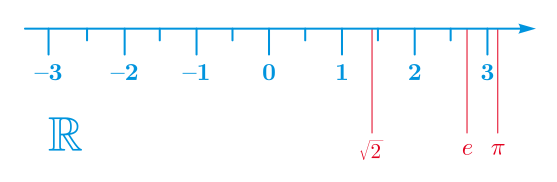
\includegraphics{img/topologia-reales/recta-real.png}

}

\caption{La recta real}

\end{figure}

\hypertarget{intervalos-y-entornos}{%
\section{Intervalos y entornos}\label{intervalos-y-entornos}}

\begin{definition}[Intervalo
abierto]\protect\hypertarget{def-intervalo-abierto}{}\label{def-intervalo-abierto}

Dados dos números reales tales que \(a\leq b\), se llama \emph{intervalo
abierto} de extremos \(a\) y \(b\), y se denota \((a,b)\) al conjunto de
números reales comprendidos entre \(a\) y \(b\) \[
(a,b) = \{x\in \mathbb{R}: a<x<b\}.
\]

\end{definition}

\begin{definition}[Intervalo
cerrado]\protect\hypertarget{def-intervalo-cerrado}{}\label{def-intervalo-cerrado}

Dados dos números reales tales que \(a\leq b\), se llama \emph{intervalo
cerrado} de extremos \(a\) y \(b\), y se denota \([a,b]\) al conjunto de
números reales que son mayores o iguales que \(a\) y menores o iguales
que \(b\) \[
[a,b] = \{x\in \mathbb{R}: a\leq x\leq b\}.
\]

\end{definition}

\begin{tcolorbox}[enhanced jigsaw, colback=white, colbacktitle=quarto-callout-warning-color!10!white, title=\textcolor{quarto-callout-warning-color}{\faExclamationTriangle}\hspace{0.5em}{Advertencia}, rightrule=.15mm, coltitle=black, arc=.35mm, opacityback=0, colframe=quarto-callout-warning-color-frame, bottomtitle=1mm, titlerule=0mm, toptitle=1mm, bottomrule=.15mm, toprule=.15mm, breakable, opacitybacktitle=0.6, left=2mm, leftrule=.75mm]

Obsérvese que si \(a=b\), \((a,a)=\emptyset\) y \([a,a]=\{a\}\).

\end{tcolorbox}

Los intervalos también pueden ser abiertos por un lado y cerrados por el
otro.

\begin{definition}[Intervalo semiabierto o
semicerrado]\protect\hypertarget{def-intervalo-semiabierto}{}\label{def-intervalo-semiabierto}

Dados dos números reales tales que \(a<b\), se definen los
\emph{intervalos semiabiertos} o \emph{semicerrados} de extremos \(a\) y
\(b\) de la siguiente manera: \[
(a,b] = \{x\in \mathbb{R}: a< x\leq b\}\quad \mbox{y}\quad [a,b) = \{x\in \mathbb{R}: a\leq x< b\}
\]

\end{definition}

Estos intervalos están \emph{acotados} ya que \(a\) es una cota inferior
y \(b\) una cota superior, pero también existen intervalos no acotados.

\begin{definition}[Intervalo abierto no
acotado]\protect\hypertarget{def-intervalo-abierto-no-acotado}{}\label{def-intervalo-abierto-no-acotado}

Dado un número \(a\in \mathbb{R}\), se definen los siguientes
\emph{intervalos abiertos no acotados}: \[
(-\infty,a) = \{x\in \mathbb{R}: x<a\} \quad \mbox{y}\quad (a,\infty) = \{x\in \mathbb{R}: a< x\}
\]

\end{definition}

\begin{definition}[Intervalo semiabierto no
acotado]\protect\hypertarget{def-intervalo-semiabierto-no-acotado}{}\label{def-intervalo-semiabierto-no-acotado}

Dado un número \(a\in \mathbb{R}\), se definen los siguientes
\emph{intervalos semiabiertos no acotados}: \[
(-\infty,a] = \{x\in \mathbb{R}: x\leq a\} \quad \mbox{y}\quad [a,\infty) = \{x\in \mathbb{R}: a\leq x\}
\]

\end{definition}

\begin{definition}[Intervalos
anidados]\protect\hypertarget{def-intervalos-anidados}{}\label{def-intervalos-anidados}

Se dice que una sucesión de intervalos \(I_n\), \(n\in\mathbb{N}\) es
una \emph{sucesión de intervalos anidados} si se cumple que
\(I_{n+1}\subseteq I_n\) \(\forall n\in\mathbb{N}\).

\end{definition}

\begin{example}[]\protect\hypertarget{exm-sucesion-intervalos-anidados}{}\label{exm-sucesion-intervalos-anidados}

La sucesión de intervalos \(I_n=[0,\frac{1}{n}]\),
\(\forall n\in\mathbb{N}\) es una sucesión de intervalos anidados, ya
que para cada \(n\in\mathbb{N}\) se cumple que \(n<n+1\) y por tanto
\(\frac{1}{n}>\frac{1}{n+1}\), de manera que
\(I_{n+1}=[0,\frac{1}{n+1}]\subseteq [0,\frac{1}{n}]=I_n\).

\end{example}

\begin{theorem}[Intervalos
anidados]\protect\hypertarget{thm-intervalos-anidados}{}\label{thm-intervalos-anidados}

Dada una sucesión de intervalos cerrados y anidados \(I_n=[a_n,b_n]\),
\(n\in\mathbb{N}\), existe un número \(a\in\mathbb{R}\) tal que
\(a\in I_n\) \(\forall n\in\mathbb{N}\). Además, si el ínfimo de las
longitudes \(\{b_n-a_n: n\in \mathbb{N}\}\) es \(0\), entonces \(a\) es
único, es decir, \(\cap_{n=1}^\infty I_n=\{a\}\).

\end{theorem}

\begin{tcolorbox}[enhanced jigsaw, colback=white, colbacktitle=quarto-callout-note-color!10!white, title=\textcolor{quarto-callout-note-color}{\faInfo}\hspace{0.5em}{Demostración}, rightrule=.15mm, coltitle=black, arc=.35mm, opacityback=0, colframe=quarto-callout-note-color-frame, bottomtitle=1mm, titlerule=0mm, toptitle=1mm, bottomrule=.15mm, toprule=.15mm, breakable, opacitybacktitle=0.6, left=2mm, leftrule=.75mm]

\begin{proof}

Sea \(A=\{a_n: n\in\mathbb{N}\}\) y \(B=\{b_n: n\in\mathbb{N}\}\).
Puesto que los intervalos están anidados, \(A\) está acotado
superiormente por \(b_1\) ya que \(a_n\leq b_n\leq b_1\)
\(\forall n\in \mathbb{N}\), y \(B\) está acotado inferiormente por
\(a_1\) ya que \(a_1\leq a_n\leq b_n\) \(\forall n\in \mathbb{N}\). Así
pues, como \(A\) está acotado superiormente, por el axioma del supremo,
existe \(a=\sup(A)\), y como \(B\) está acotado inferiormente, existe
\(b=\inf(B)\).

Veamos ahora que \(a\leq b\). Para ello basta probar que \(a\) es cota
inferior de \(B\). Para cualquier \(n\in\mathbb{N}\) se cumple que si
\(k\geq n\) entonces \(a_k\leq b_k\leq b_n\) pues \(I_n\subseteq I_k\),
y si \(k<n\), entonces \(a_k\leq a_n\leq b_n\), pues
\(I_n\subseteq I_k\). Luego \(b_n\) es una cota superior de \(A\), y por
tanto, \(a\leq b_n\) \(\forall n\in\mathbb{N}\), de manera que \(a\) es
cota inferior de \(B\). Así pues, como \(a\) es cota superior de \(A\) e
inferior de \(B\), se tiene que \(a_n\leq a\leq b_n\)
\(\forall n\in\mathbb{N}\), de manera que
\(a\in \cap_{n=1}^\infty I_n\).

De forma similar se puede probar que \(b\in \cap_{n=1}^\infty I_n\), por
lo que \(\cap_{n=1}^\infty I_n = [a,b]\).

Finalmente, veamos que si \(\inf(\{b_n-a_n: n\in \mathbb{N}\})=0\)
entonces \(a=b\). Para ello, dado \(\varepsilon>0\), como
\(\inf(\{b_n-a_n: n\in \mathbb{N}\})=0\), existe \(k\in\mathbb{N}\) tal
que \(0\leq b_k-a_k < \varepsilon\). Como \(b\leq b_k\) y \(a\geq a_k\),
se tiene que \(0\leq b-a\leq b_k-a_k < \varepsilon\), de donde se deduce
que \(b-a=0\) y por tanto \(a=b\), así que
\(\cap_{n=1}^\infty I_n = [a,a]=\{a\}\).

\end{proof}

\end{tcolorbox}

\begin{definition}[Entorno]\protect\hypertarget{def-entorno}{}\label{def-entorno}

Dado un número \(a\in \mathbb{R}\), se llama \emph{entorno} de \(a\) a
cualquier intervalo abierto \((a-\varepsilon, a+\varepsilon)\) con
\(\varepsilon>0\). El número \(\varepsilon\) se conoce como \emph{radio
del entorno}.

Para cualquier \(\varepsilon>0\) el conjunto
\((a-\varepsilon, a+\varepsilon)\setminus \{a\}\) se llama \emph{entorno
reducido} de \(a\).

\end{definition}

\hypertarget{clasificaciuxf3n-de-puntos}{%
\section{Clasificación de puntos}\label{clasificaciuxf3n-de-puntos}}

Un conjunto \(A\subset \mathbb{R}\) clasifica los puntos de
\(\mathbb{R}\) en tres clases: puntos interiores, puntos exteriores y
puntos fronteras de \(A\).

\begin{definition}[Punto
interior]\protect\hypertarget{def-punto-interior}{}\label{def-punto-interior}

Se dice que \(a\in \mathbb{R}\) es un \emph{punto interior} de un
conjunto \(A\subseteq \mathbb{R}\), si existe un entorno de \(a\)
contenido en \(A\), es decir, existe \(\varepsilon>0\) tal que
\((a-\varepsilon, a+\varepsilon) \subseteq A\).

El conjunto de los puntos interiores de \(A\) se llama \emph{interior}
de \(A\) y se denota por \(\operatorname{Int}(A)\).

\end{definition}

Aunque la definición no lo hace explícito, es evidente que si \(a\) es
un punto interior de \(A\) entonces \(a\in A\).

Intuitivamente, un punto interior de un conjunto es un punto que no está
en el borde del conjunto, es decir, que está rodeado por puntos del
conjunto, y por tanto, podemos movernos un poco hacia la izquierda o
hacia la derecha del punto sin salirnos del conjunto.

\begin{example}[]\protect\hypertarget{exm-punto-interior}{}\label{exm-punto-interior}

\(0.9\) es un punto interior del intervalo \((0,1)\) ya que podemos
tomar \(\varepsilon = 0.01\) tal que el entorno
\((0.9-0.01,0.9+0.01) = (0.89, 0.91)\subset (0,1)\).

Sin embargo, \(1\) no es un punto interior del intervalo \((0,1)\) ya
que por muy pequeño que tomemos \(\varepsilon>0\), \(1+\varepsilon > 1\)
y, por tanto, el entorno \((1-\varepsilon, 1+\varepsilon)\) siempre
tendrá valores mayores que 1, de manera que
\((1-\varepsilon, 1+\varepsilon)\not \subseteq (0,1)\).

\end{example}

\begin{definition}[Punto
exterior]\protect\hypertarget{def-punto-exterior}{}\label{def-punto-exterior}

Se dice que \(a\in \mathbb{R}\) es un \emph{punto exterior} de un
conjunto \(A\subseteq \mathbb{R}\), si existe un entorno de \(a\)
contenido en el complementario de \(A\), es decir, existe
\(\varepsilon>0\) tal que
\((x-\varepsilon, x+\varepsilon) \subseteq \overline A\).

El conjunto de los puntos exteriores de \(A\) se llama \emph{exterior}
de \(A\) y se denota por \(\operatorname{Ext}(A)\).

\end{definition}

Una definición equivalente es que un punto es punto exterior de un
conjunto si es un punto interior de su complementario.

\begin{example}[]\protect\hypertarget{exm-punto-exterior}{}\label{exm-punto-exterior}

\(1.01\) es un punto exterior del conjunto \((-\infty, 1)\) ya que
tomando \(\varepsilon=0.001\) el entorno
\((1.01-0.001, 1.01+0.001)=(1.009, 1.011)\in \overline{(-\infty, 1)}=[1,\infty)\).

Sin embargo, \(1\) no es un punto exterior del intervalo
\((-\infty, 1)\), ya que no es un punto interior del intervalo
\(\overline{(-\infty, 1)}=[1,\infty)\), ya que \(1-\varepsilon < 1\)
\(\forall \varepsilon>0\), y, por tanto, el entorno
\((1-\varepsilon, 1+\varepsilon)\) siempre tendrá valores menores que 1,
de manera que
\((1-\varepsilon, 1+\varepsilon)\not \subseteq [1,\infty)\).

\end{example}

\begin{tcolorbox}[enhanced jigsaw, colback=white, colbacktitle=quarto-callout-warning-color!10!white, title=\textcolor{quarto-callout-warning-color}{\faExclamationTriangle}\hspace{0.5em}{Advertencia}, rightrule=.15mm, coltitle=black, arc=.35mm, opacityback=0, colframe=quarto-callout-warning-color-frame, bottomtitle=1mm, titlerule=0mm, toptitle=1mm, bottomrule=.15mm, toprule=.15mm, breakable, opacitybacktitle=0.6, left=2mm, leftrule=.75mm]

El que un punto no sea punto interior de un conjunto no significa que
sea un punto exterior. Por ejemplo, \(1\) no es un punto interior del
intervalo \((0,1)\), y tampoco de su complementario
\(\overline{(0,1)}=(-\infty, 0]\cup[1,\infty)\).

\end{tcolorbox}

\begin{definition}[Punto
frontera]\protect\hypertarget{def-punto-frontera}{}\label{def-punto-frontera}

Se dice que \(a\in \mathbb{R}\) es un \emph{punto frontera} de un
conjunto \(A\subseteq \mathbb{R}\), si cualquier entorno de \(a\)
contiene puntos de \(A\) y de su complementario.

El conjunto de los puntos frontera de \(A\) se llama \emph{frontera} de
\(A\) y se denota por \(\operatorname{Fr}(A)\).

\end{definition}

Una definición equivalente es que un punto es un punto frontera de un
conjunto si no es un punto interior ni exterior del conjunto.

\begin{example}[]\protect\hypertarget{exm-punto-frontera}{}\label{exm-punto-frontera}

El punto \(1\) es un punto frontera del intervalo \([1,\infty)\) ya que
no es un punto interior de \([1,\infty)\) ni de su complementario
\((-\infty,1)\).

\end{example}

\begin{proposition}[]\protect\hypertarget{prp-interior-intervalo-abierto}{}\label{prp-interior-intervalo-abierto}

Todos los puntos de un intervalo abierto son puntos interiores suyos, es
decir, dado un intervalo abierto \((a,b)\subseteq \mathbb{R}\), se
cumple que \(\operatorname{Int}((a,b)) = (a,b)\).

\end{proposition}

\begin{tcolorbox}[enhanced jigsaw, colback=white, colbacktitle=quarto-callout-note-color!10!white, title=\textcolor{quarto-callout-note-color}{\faInfo}\hspace{0.5em}{Demostración}, rightrule=.15mm, coltitle=black, arc=.35mm, opacityback=0, colframe=quarto-callout-note-color-frame, bottomtitle=1mm, titlerule=0mm, toptitle=1mm, bottomrule=.15mm, toprule=.15mm, breakable, opacitybacktitle=0.6, left=2mm, leftrule=.75mm]

\begin{proof}

Tomemos cualquier punto \(x\in (a,b)\), entonces se puede tomar
\(\varepsilon = \frac{\min\{|x-a|,|x-b\}}{2}\) de manera que el entorno
\((x-\varepsilon, x+\varepsilon)\subseteq (a,b)\).

\end{proof}

\end{tcolorbox}

\begin{proposition}[]\protect\hypertarget{prp-interior-intervalo-cerrado}{}\label{prp-interior-intervalo-cerrado}

Todos los puntos de un intervalo cerrado, excepto sus extremos, son
puntos interiores suyos, es decir, dado un intervalo cerrado
\([a,b]\subseteq \mathbb{R}\), se cumple que
\(\operatorname{Int}([a,b]) = (a,b)\).

\end{proposition}

\begin{tcolorbox}[enhanced jigsaw, colback=white, colbacktitle=quarto-callout-note-color!10!white, title=\textcolor{quarto-callout-note-color}{\faInfo}\hspace{0.5em}{Demostración}, rightrule=.15mm, coltitle=black, arc=.35mm, opacityback=0, colframe=quarto-callout-note-color-frame, bottomtitle=1mm, titlerule=0mm, toptitle=1mm, bottomrule=.15mm, toprule=.15mm, breakable, opacitybacktitle=0.6, left=2mm, leftrule=.75mm]

\begin{proof}

Par ver que \(a\) no es un punto interior de \([a,b]\), basta con ver
que \(a-\varepsilon < a\) para cualquier \(\varepsilon>0\), por lo que
el intervalo \((a-\varepsilon,a+\varepsilon)\) irremediablemente
contendrá puntos menores que \(a\) y, por tanto,
\((a-\varepsilon,a+\varepsilon)\not \subseteq [a,b]\).

Un razonamiento análogo se puede utilizar para demostrar que \(b\)
tampoco es un punto interior de \([a,b]\).

\end{proof}

\end{tcolorbox}

A partir de estas proposiciones, es fácil ver que que para cualquier
intervalo abierto \((a,b)\), \(\operatorname{Int}((a,b)) = (a,b)\),
\(\operatorname{Ext}((a,b)) = (-\infty,a)\cup (b,\infty)\) y
\(\operatorname{Fr}((a,b)) = \{a, b\}\). Y para cualquier intervalo
cerrado \([a,b]\), \(\operatorname{Int}([a,b]) = (a,b)\),
\(\operatorname{Ext}([a,b]) = (-\infty,a)\cup (b,\infty)\) y
\(\operatorname{Fr}([a,b]) = \{a, b\}\).

\begin{proposition}[]\protect\hypertarget{prp-clasifiacion-puntos}{}\label{prp-clasifiacion-puntos}

Dado un conjunto \(A\subset \mathbb{R}\), los conjuntos
\(\operatorname{Int}(A)\), \(\operatorname{Ext}(A)\) y
\(\operatorname{Fr}(A)\) forman una partición de \(\mathbb{R}\), es
decir,

\begin{enumerate}
\def\labelenumi{\alph{enumi}.}
\tightlist
\item
  \(\operatorname{Int}(A)\), \(\operatorname{Ext}(A)\) y
  \(\operatorname{Fr}(A)\) son disjuntos entre sí.
\item
  \(\operatorname{Int}(A)\cup \operatorname{Ext}(A)\cup \operatorname{Fr}(A) = \mathbb{R}\).
\end{enumerate}

\end{proposition}

\begin{tcolorbox}[enhanced jigsaw, colback=white, colbacktitle=quarto-callout-note-color!10!white, title=\textcolor{quarto-callout-note-color}{\faInfo}\hspace{0.5em}{Demostración}, rightrule=.15mm, coltitle=black, arc=.35mm, opacityback=0, colframe=quarto-callout-note-color-frame, bottomtitle=1mm, titlerule=0mm, toptitle=1mm, bottomrule=.15mm, toprule=.15mm, breakable, opacitybacktitle=0.6, left=2mm, leftrule=.75mm]

\begin{proof}

Se deja como ejercicio.

\end{proof}

\end{tcolorbox}

A continuación se definen otros tipos de puntos que son útiles para
definir conceptos que se verán más adelante como el de \emph{límite}.

\begin{definition}[Punto
adherente]\protect\hypertarget{def-punto-adherente}{}\label{def-punto-adherente}

Se dice que \(a\in \mathbb{R}\) es un \emph{punto adherente} de un
conjunto \(A\subseteq \mathbb{R}\), si cualquier entorno de \(a\)
contiene puntos de \(A\).

El conjunto de los puntos adherentes de \(A\) se llama \emph{adherencia}
de \(A\) y se denota por \(\operatorname{Adh}(A)\).

\end{definition}

Resulta obvio que cualquier punto interior y frontera de un conjunto es
también adherente, y que cualquier punto exterior no es adherente.
Resulta evidente también que cualquier punto de un conjunto es un punto
adherente, de manera que para cualquier conjunto \(A\) se tiene
\(A\subseteq\operatorname{Adh}(A)\).

\begin{definition}[Punto de
acumulacion]\protect\hypertarget{def-punto-acumulacion}{}\label{def-punto-acumulacion}

Se dice que \(a\in \mathbb{R}\) es un \emph{punto de acumulación} de un
conjunto \(A\subseteq \mathbb{R}\), si cualquier entorno reducido de
\(a\) contiene puntos de \(A\).

El conjunto de los puntos de acumulación de \(A\) se llama
\emph{conjunto derivado} de \(A\) y se denota por
\(\operatorname{Ac}(A)\).

\end{definition}

\begin{tcolorbox}[enhanced jigsaw, colback=white, colbacktitle=quarto-callout-warning-color!10!white, title=\textcolor{quarto-callout-warning-color}{\faExclamationTriangle}\hspace{0.5em}{Advertencia}, rightrule=.15mm, coltitle=black, arc=.35mm, opacityback=0, colframe=quarto-callout-warning-color-frame, bottomtitle=1mm, titlerule=0mm, toptitle=1mm, bottomrule=.15mm, toprule=.15mm, breakable, opacitybacktitle=0.6, left=2mm, leftrule=.75mm]

Resulta obvio de la definición que cualquier punto de acumulación es
también un punto de adherencia, es decir,
\(\operatorname{Ac}(A)\subseteq \operatorname{Adh}(A)\) para cualquier
conjunto \(A\subset \mathbb{R}\). Sin embargo no todo punto de
adherencia es un punto de acumulación.

\end{tcolorbox}

Es posible que un conjunto tenga puntos de acumulación que pertenezcan
al conjunto y otros que no.

\begin{example}[]\protect\hypertarget{exm-puntos-adherentes-acumulacion}{}\label{exm-puntos-adherentes-acumulacion}

Dado el conjunto \(A=(0,1) \cup \{2\}\), se tiene que \(2\) es un punto
de adherencia de \(A\), pues para cualquier \(\varepsilon>0\) el entorno
\((2-\varepsilon,2+\varepsilon)\) contiene al propio \(2\) que es un
punto de \(A\). Sin embargo, \(2\) no es un punto de acumulación, porque
para \(\varepsilon=0.5\), por ejemplo, el entorno reducido
\((2-\varepsilon,2+\varepsilon)\setminus\{2\}=(1.5,2)\cup(2,2.5)\) no
contiene puntos de \(A\).

En cambio el punto \(0.5\) es tanto un punto de adherencia como un punto
de acumulación de \(A\) porque para cualquier \(\varepsilon>0\) el
entorno reducido \((0.5-\varepsilon,0.5+\varepsilon)\setminus \{0.5\}\)
siempre contiene puntos de \(A\). De hecho, para cualquier \(x\in(a,b)\)
y para cualquier \(\varepsilon>0\), el intervalo
\((x-\varepsilon,x+\varepsilon)\setminus \{x\}\) contiene puntos de
\(A\), y lo mismo ocurre para \(a\) y \(b\) al ser puntos frontera, de
manera que \(\operatorname{Ac}(A)=[0,1]\), mientras que
\(\operatorname{Adh}(A)=[0,1]\cup\{2\}\).

\end{example}

Intuitivamente, un punto de acumulación de un conjunto \(A\) es un punto
para el que podemos encontrar puntos de \(A\), distintos de él mismo,
tan próximos a él como queramos. Un punto de acumulación se diferencia
de un punto de adherencia en que siempre está rodeado por puntos de
\(A\), mientras que un punto de adherencia puede estar aislado de los
demás puntos de \(A\).

\begin{definition}[Punto
aislado]\protect\hypertarget{def-punto-aislado}{}\label{def-punto-aislado}

Se dice que \(a\in \mathbb{R}\) es un \emph{punto de aislado} de un
conjunto \(A\subseteq \mathbb{R}\), si es un punto adherente de \(A\),
pero no de acumulación.

\end{definition}

\begin{proposition}[]\protect\hypertarget{prp-punto-adherente-acumulacion}{}\label{prp-punto-adherente-acumulacion}

Para cualquier intervalo abierto \((a,b)\) se tiene que
\(\operatorname{Adh}((a,b))=\operatorname{Ac}((a,b))=[a,b]\).

\end{proposition}

\begin{tcolorbox}[enhanced jigsaw, colback=white, colbacktitle=quarto-callout-note-color!10!white, title=\textcolor{quarto-callout-note-color}{\faInfo}\hspace{0.5em}{Demostración}, rightrule=.15mm, coltitle=black, arc=.35mm, opacityback=0, colframe=quarto-callout-note-color-frame, bottomtitle=1mm, titlerule=0mm, toptitle=1mm, bottomrule=.15mm, toprule=.15mm, breakable, opacitybacktitle=0.6, left=2mm, leftrule=.75mm]

\begin{proof}

Todos los puntos de \((a,b)\) son interiores y, por tanto, para
cualquier \(x\in (a,b)\), existe un \(\varepsilon>0\) tal que
\((x-\varepsilon,x+\varepsilon)\subseteq (a,b)\). Si ahora tomamos
cualquier otro \(\varepsilon'>0\), se tiene que
\((x-\varepsilon',x+\varepsilon')\setminus \{x\}\cap(x-\varepsilon,x+\varepsilon)\neq \emptyset\),
pero como \((x-\varepsilon,x+\varepsilon)\subseteq (a,b)\), se concluye
que
\((x-\varepsilon',x+\varepsilon')\setminus \{x\}\cap (a,b)\neq \emptyset\),
por lo que \(x\) es un punto de acumulación de \((a,b)\). Por otro lado,
como \(a\) y \(b\) son puntos frontera, también se tiene que para
cualquier \(\varepsilon>0\),
\((a-\varepsilon,a+\varepsilon)\cap (a,b)\neq \emptyset\) y
\((b-\varepsilon,b+\varepsilon)\cap (a,b)\neq \emptyset\) de manera que
\([a,b]\subseteq \operatorname{Ac}((a,b))\subseteq \operatorname{Adh}((a,b))\).
Sea ahora cualquier \(x>b\), y tomemos \(\varepsilon=\frac{|x-b|}{2}\),
entonces \((x-\varepsilon, x+\varepsilon)\cap (a,b)=\emptyset\), de
manera que \(x\) no es un punto de adherencia de \((a,b)\). Del mismo
modo se puede probar que si \(x<a\), entonces \(x\) tampoco es un punto
de adherencia de \((a,b)\), por lo que
\(\operatorname{Adh}((a,b))=[a,b]\) y como
\(\operatorname{Ac}((a,b))\subseteq \operatorname{Adh}((a,b))\), también
se concluye que \(\operatorname{Ac}((a,b))=[a,b]\).

\end{proof}

\end{tcolorbox}

\begin{proposition}[]\protect\hypertarget{prp-adherencia-conjunto-mas-acumulacion}{}\label{prp-adherencia-conjunto-mas-acumulacion}

Para cualquier conjunto \(A\subseteq \mathbb{R}\), se tiene que
\(\operatorname{Adh}(A)=A\cup \operatorname{Ac}(A)\).

\end{proposition}

\begin{tcolorbox}[enhanced jigsaw, colback=white, colbacktitle=quarto-callout-note-color!10!white, title=\textcolor{quarto-callout-note-color}{\faInfo}\hspace{0.5em}{Demostración}, rightrule=.15mm, coltitle=black, arc=.35mm, opacityback=0, colframe=quarto-callout-note-color-frame, bottomtitle=1mm, titlerule=0mm, toptitle=1mm, bottomrule=.15mm, toprule=.15mm, breakable, opacitybacktitle=0.6, left=2mm, leftrule=.75mm]

\begin{proof}

Ya se ha visto que \(A\subseteq \operatorname{Adh}(A)\) y también
\(\operatorname{Ac}(A)\subseteq \operatorname{Adh}(A)\), por lo que
\(A\cup \operatorname{Ac}(A)\subseteq \operatorname{Adh}(A)\).

Veamos ahora que
\(\operatorname{Adh}(A)\subseteq A\cup \operatorname{Ac}(A)\). Sea \(x\)
un punto de adherencia de \(A\). Si \(x\in A\) es obvio que
\(x\in A\cup \operatorname{Ac}(A)\), y si \(x\not\in A\), entonces
\(x\in \operatorname{Ac}(A)\), ya que, por ser \(x\) punto de adherencia
de \(A\), para cualquier \(\varepsilon>0\),
\((x-\varepsilon,x+\varepsilon)\cap A\neq \emptyset\), pero como además
\(x\not\in A\), también se cumple que el entorno reducido
\((x-\varepsilon,x+\varepsilon)\setminus\{x\}\) contiene puntos de
\(A\). Así pues, \(x\in A\cup \operatorname{Ac}(A)\), y por tanto
\(\operatorname{Adh}(A)\subseteq A\cup \operatorname{Ac}(A)\).

\end{proof}

\end{tcolorbox}

\hypertarget{conjuntos-abiertos-y-cerrados}{%
\section{Conjuntos abiertos y
cerrados}\label{conjuntos-abiertos-y-cerrados}}

A continuación se generaliza la característica que diferencia los
intervalos abiertos y cerrados, a cualquier conjunto.

\begin{definition}[Conjunto
abierto]\protect\hypertarget{def-conjunto-abierto}{}\label{def-conjunto-abierto}

Se dice que un conjunto \(A\subset \mathbb{R}\) es \emph{abierto} cuando
para cada \(a\in A\) existe un entorno de \(a\) contenido en \(A\), es
decir, existe \(\varepsilon>0\) tal que
\((a-\varepsilon, a+\varepsilon)\subset A\).

\end{definition}

\begin{tcolorbox}[enhanced jigsaw, colback=white, colbacktitle=quarto-callout-important-color!10!white, title=\textcolor{quarto-callout-important-color}{\faExclamation}\hspace{0.5em}{Importante}, rightrule=.15mm, coltitle=black, arc=.35mm, opacityback=0, colframe=quarto-callout-important-color-frame, bottomtitle=1mm, titlerule=0mm, toptitle=1mm, bottomrule=.15mm, toprule=.15mm, breakable, opacitybacktitle=0.6, left=2mm, leftrule=.75mm]

Obsérvese que un conjunto es abierto si todos sus puntos son interiores.

\end{tcolorbox}

\begin{example}[]\protect\hypertarget{exm-intervalo-abierto-conjunto-abierto}{}\label{exm-intervalo-abierto-conjunto-abierto}

Cualquier intervalo abierto \((a,b)\) es un conjunto abierto, ya que
según se vio en la Proposición~\ref{prp-interior-intervalo-abierto}
\(\operatorname{Int}((a,b)) = (a,b)\). Por otro lado, un intervalo
cerrado \([a,b]\) no es un conjunto abierto pues cualquier entorno de
\(a\) o \(b\) no está contenido en \([a,b]\).

\end{example}

Una colección de conjuntos abiertos se llama \emph{topología} y
cualquier propiedad que pueda definirse en términos de conjuntos
abiertos se llama \emph{propiedad topológica}.

\begin{definition}[Conjunto
cerrado]\protect\hypertarget{def-conjunto-cerrado}{}\label{def-conjunto-cerrado}

Se dice que un conjunto \(A\subset \mathbb{R}\) es \emph{cerrado} cuando
su complementario \(\overline A =\mathbb{R}\setminus A\) es abierto.

\end{definition}

\begin{example}[]\protect\hypertarget{exm-intervalo-cerrado-conjunto-cerrado}{}\label{exm-intervalo-cerrado-conjunto-cerrado}

Todo intervalo cerrado \([a,b]\) es cerrado, pues su complementario
\((-\infty,a)\cup (b,\infty)\) es abierto.

\end{example}

\begin{tcolorbox}[enhanced jigsaw, colback=white, colbacktitle=quarto-callout-warning-color!10!white, title=\textcolor{quarto-callout-warning-color}{\faExclamationTriangle}\hspace{0.5em}{Advertencia}, rightrule=.15mm, coltitle=black, arc=.35mm, opacityback=0, colframe=quarto-callout-warning-color-frame, bottomtitle=1mm, titlerule=0mm, toptitle=1mm, bottomrule=.15mm, toprule=.15mm, breakable, opacitybacktitle=0.6, left=2mm, leftrule=.75mm]

Un subconjunto puede ser abierto y cerrado a la vez, como por ejemplo
\(\mathbb{R}\) y \(\emptyset\). \(\mathbb{R}\) es abierto ya que todos
sus puntos son interiores, y por tanto
\(\overline{\mathbb{R}}=\emptyset\) es cerrado. Pero, también
\(\emptyset\) es abierto, ya que para que un conjunto no sea abierto, al
menos uno de sus puntos no debe ser interior, y en consecuencia
\(\overline{\emptyset}=\mathbb{R}\) es también cerrado.

Un subconjunto también puede no ser abierto ni cerrado, como por ejemplo
\((a,b]\), ya que \(b\) no es un punto interior de \((a,b]\), y \(a\) no
es un punto interior de \(\overline{(a,b]}=(-\infty,a]\cup (b,\infty)\).
Por tanto, no abierto no implica cerrado y no cerrado no implica
abierto.

\end{tcolorbox}

\begin{proposition}[]\protect\hypertarget{prp-union-interseccion-conjuntos-abiertos-cerrados}{}\label{prp-union-interseccion-conjuntos-abiertos-cerrados}

Se cumplen las siguientes propiedades:

\begin{enumerate}
\def\labelenumi{\arabic{enumi}.}
\tightlist
\item
  La unión de una colección de conjuntos abiertos es un conjunto
  abierto.
\item
  La intersección de una colección finita de conjuntos abiertos es un
  conjunto abierto.
\item
  La intersección de una colección de conjuntos cerrados es cerrada.
\item
  La unión de una colección finita de conjuntos cerrados es un conjunto
  cerrado.
\end{enumerate}

\end{proposition}

\begin{tcolorbox}[enhanced jigsaw, colback=white, colbacktitle=quarto-callout-note-color!10!white, title=\textcolor{quarto-callout-note-color}{\faInfo}\hspace{0.5em}{Demostración}, rightrule=.15mm, coltitle=black, arc=.35mm, opacityback=0, colframe=quarto-callout-note-color-frame, bottomtitle=1mm, titlerule=0mm, toptitle=1mm, bottomrule=.15mm, toprule=.15mm, breakable, opacitybacktitle=0.6, left=2mm, leftrule=.75mm]

\begin{proof}

Se deja como ejercicio.

\end{proof}

\end{tcolorbox}

\begin{tcolorbox}[enhanced jigsaw, colback=white, colbacktitle=quarto-callout-warning-color!10!white, title=\textcolor{quarto-callout-warning-color}{\faExclamationTriangle}\hspace{0.5em}{Advertencia}, rightrule=.15mm, coltitle=black, arc=.35mm, opacityback=0, colframe=quarto-callout-warning-color-frame, bottomtitle=1mm, titlerule=0mm, toptitle=1mm, bottomrule=.15mm, toprule=.15mm, breakable, opacitybacktitle=0.6, left=2mm, leftrule=.75mm]

La intersección de una colección infinita de conjuntos abiertos puede no
ser un conjunto abierto, como por ejemplo la colección de conjuntos
\(I_n=(0,1+\frac{1}{n})\), \(n\in\mathbb{N}\), ya que
\(\cap_{n=1}^\infty I_n=(0,1]\).

Y la unión de una colección infinita de conjuntos cerrados puede no ser
cerrada, como por ejemplo la colección de conjuntos
\(J_n=[\frac{1}{n},1]\), \(n\in\mathbb{N}\), ya que
\(\cup_{n=1}^\infty J_n=(0,1]\).

\end{tcolorbox}

\begin{theorem}[Existencia del máximo y
mínimo]\protect\hypertarget{thm-existencia-maximo-minimo}{}\label{thm-existencia-maximo-minimo}

Cualquier conjunto no-vacío, cerrado y acotado superiormente tiene un
máximo, y cualquier conjunto no-vacío, cerrado y acotado inferiormente
tiene un mínimo.

\end{theorem}

\begin{tcolorbox}[enhanced jigsaw, colback=white, colbacktitle=quarto-callout-note-color!10!white, title=\textcolor{quarto-callout-note-color}{\faInfo}\hspace{0.5em}{Demostración}, rightrule=.15mm, coltitle=black, arc=.35mm, opacityback=0, colframe=quarto-callout-note-color-frame, bottomtitle=1mm, titlerule=0mm, toptitle=1mm, bottomrule=.15mm, toprule=.15mm, breakable, opacitybacktitle=0.6, left=2mm, leftrule=.75mm]

\begin{proof}

Sea \(A\) un conjunto no vacío, cerrado y acotado superiormente. Como
\(A\) está acotado superiormente, por el axioma del supremo, existe
\(s=\sup(A)\). Probaremos que \(s\in A\) por reducción al absurdo.
Supongamos que \(s\not\in A\), entonces \(s\in\overline{A}\), y como
\(\overline{A}\) es abierto al ser \(A\) cerrado, existe un
\(\varepsilon>0\) tal que
\((s-\varepsilon, s+\varepsilon)\subseteq \overline{A}\). Como ningún
elemento de \(A\) puede ser mayor que \(s\) y
\((s-\varepsilon, s+\varepsilon)\not\subseteq A\), se tiene que
\(s-\varepsilon\) es también una cota superior de \(A\), pero
\(s-\varepsilon <s\), lo que contradice que \(s\) sea el supremo de
\(A\). Así, pues \(s\in A\), y por tanto es el máximo de \(A\).

De manera análoga se prueba que si \(A\) un conjunto no vacío, cerrado y
acotado inferiormente, \(A\) tiene mínimo.

\end{proof}

\end{tcolorbox}

\begin{theorem}[Bolzano-Weierstrass]\protect\hypertarget{thm-bolzano-weierstrass}{}\label{thm-bolzano-weierstrass}

Todo subconjunto infinito de \(\mathbb{R}\) acotado tiene al menos un
punto de acumulación.

\end{theorem}

\begin{tcolorbox}[enhanced jigsaw, colback=white, colbacktitle=quarto-callout-note-color!10!white, title=\textcolor{quarto-callout-note-color}{\faInfo}\hspace{0.5em}{Demostración}, rightrule=.15mm, coltitle=black, arc=.35mm, opacityback=0, colframe=quarto-callout-note-color-frame, bottomtitle=1mm, titlerule=0mm, toptitle=1mm, bottomrule=.15mm, toprule=.15mm, breakable, opacitybacktitle=0.6, left=2mm, leftrule=.75mm]

\begin{proof}

Para demostrar el teorema construiremos una sucesión de intervalos
cerrados y anidados y aplicaremos el
Teorema~\ref{thm-intervalos-anidados}.

Sea \(A\subset \mathbb{R}\) un subconjunto infinito y acotado. Como
\(A\) está acotado, existe un intervalo cerrado tal que
\(A\subset I_1=[a_1,b_1]\). Si \(I_1\) se divide en dos intervalos
\([a_1, \frac{a_1+b_1}{2}]\) y \([\frac{a_1+b_1}{2}, b_1]\), al menos
uno de estos intervalos tendrá infinitos puntos de \(A\), ya que de lo
contrario \(A\) sería finito. Sea \(I_2=[a_2,b_2]\) cualquiera de los
dos intervalos que tenga infinitos puntos de \(A\). Si \(I_2\) se divide
en dos intervalos \([a_2, \frac{a_2+b_2}{2}]\) y
\([\frac{a_2+b_2}{2}, b_2]\), al menos uno de estos intervalos tendrá
infinitos puntos de \(A\), ya que de lo contrario \(A\) sería finito.
Sea \(I_3=[a_3,b_3]\) cualquiera de los dos intervalos que tenga
infinitos puntos de \(A\). Siguiendo la misma lógica, se puede construir
una sucesión de intervalos anidados
\(I_1\supset I_2\supset I_3 \supset \cdots\), con tamaños
\(\frac{b_1-a_1}{2^{n-1}}\). Como
\(\inf\{\frac{b_1-a_1}{2^{n-1}}: n\in\mathbb{N}\} =0\), aplicando el
Teorema~\ref{thm-intervalos-anidados}, existe un único
\(a\in\mathbb{R}\) tal que \(\cap_{n=1}^\infty I_n=\{a\}\).

Veremos ahora que \(a\) es un punto de acumulación de \(A\). Para
cualquier \(\varepsilon>0\), considérese el entorno reducido de \(a\)
\((a-\varepsilon, a+\varepsilon)\setminus\{a\}\). Como
\(\inf\{\frac{b_1-a_1}{2^{n-1}}: n\in\mathbb{N}\} =0\), existe
\(m\in\mathbb{N}\) tal que \(\frac{b_1-a_1}{2^{m-1}}<\varepsilon\), y
por tanto \(I_m\subset (a-\varepsilon, a+\varepsilon)\), y como \(I_m\)
contiene infinitos puntos de \(A\), el entorno reducido \(a\) también
contiene puntos de \(A\), por lo que \(a\) es un punto de acumulación de
\(A\).

\end{proof}

\end{tcolorbox}

\begin{theorem}[]\protect\hypertarget{thm-conjunto-cerrado-puntos-acumulacion}{}\label{thm-conjunto-cerrado-puntos-acumulacion}

Cualquier subconjunto de \(\mathbb{R}\) es cerrado si y sólo si contiene
a todos sus puntos de acumulación.

\end{theorem}

\begin{tcolorbox}[enhanced jigsaw, colback=white, colbacktitle=quarto-callout-note-color!10!white, title=\textcolor{quarto-callout-note-color}{\faInfo}\hspace{0.5em}{Demostración}, rightrule=.15mm, coltitle=black, arc=.35mm, opacityback=0, colframe=quarto-callout-note-color-frame, bottomtitle=1mm, titlerule=0mm, toptitle=1mm, bottomrule=.15mm, toprule=.15mm, breakable, opacitybacktitle=0.6, left=2mm, leftrule=.75mm]

\begin{proof}

Sea \(A\subset \mathbb{R}\) un conjunto cerrado y sea \(a\in\mathbb{R}\)
un punto de acumulación de \(A\). Veamos por reducción al absurdo que
\(a\in A\).

Supongamos que \(a\not\in A\), entonces \(a\in \overline A\). Como \(A\)
es cerrado, \(\overline A\) es abierto y existe un \(\varepsilon>0\) tal
que el entorno \((a-\varepsilon, a+\varepsilon)\subset \overline A\),
pero entonces \((a-\varepsilon, a+\varepsilon)\cap A=\emptyset\), lo que
contradice que \(a\) sea punto de acumulación de \(A\).

Veremos ahora el otro sentido de la implicación. Sea \(A\) un conjunto
que contiene todos sus puntos de acumulación. Sea \(x\in \overline A\),
entonces \(x\not\in A\) y por tanto no es un punto de acumulación de
\(A\) y existe un \(\varepsilon>0\) tal que el entorno propio de \(x\)
\((x-\varepsilon, x+\varepsilon)\setminus\{x\}\cap A =\emptyset\). Como
\((x-\varepsilon, x+\varepsilon)\setminus\{x\}\subset \overline A\) y
\(x\in\overline{A}\) se concluye que
\((x-\varepsilon,x+\varepsilon)\subset \overline A\), de manera que
\(\overline{A}\) es abierto y \(A\) es cerrado.

\end{proof}

\end{tcolorbox}

\bookmarksetup{startatroot}

\hypertarget{sucesiones-de-nuxfameros-reales}{%
\chapter{Sucesiones de números
reales}\label{sucesiones-de-nuxfameros-reales}}

Las sucesiones de números reales son claves para comprender el concepto
de límite que es fundamental en el Análisis Matemático. En este capítulo
se presenta el concepto de sucesión de números reales, el concepto de
límite y algunos resultados importantes sobre la convergencia de
sucesiones.

\hypertarget{concepto-de-sucesiuxf3n}{%
\section{Concepto de sucesión}\label{concepto-de-sucesiuxf3n}}

\begin{definition}[Sucesión de números
reales]\protect\hypertarget{def-sucesion}{}\label{def-sucesion}

Una \emph{sucesión de números reales} es una aplicación
\(a:\mathbb{N}\to \mathbb{R}\) que asigna a cada número natural \(n\) un
número real \(a_n\), conocido como \emph{término de la sucesión}.

Utilizaremos la notación \((a_n)_{n=1}^\infty\), donde \(a_n=a(n)\) con
\(n\in\mathbb{N}\), o simplemente \(a_n\), para referirnos a la sucesión
definida por la aplicación \(a\).

\end{definition}

De manera informal, se puede decir que una sucesión es una lista
ordenada de números reales.

\begin{example}[]\protect\hypertarget{exm-sucesion1}{}\label{exm-sucesion1}

La sucesión \(\left(\frac{1}{n}\right)_{n=1}^\infty\) está formada por
los términos \(\frac{1}{1}, \frac{1}{2}, \frac{1}{3}, \ldots\).

\end{example}

\begin{tcolorbox}[enhanced jigsaw, colback=white, colbacktitle=quarto-callout-caution-color!10!white, title=\textcolor{quarto-callout-caution-color}{\faFire}\hspace{0.5em}{Precaución}, rightrule=.15mm, coltitle=black, arc=.35mm, opacityback=0, colframe=quarto-callout-caution-color-frame, bottomtitle=1mm, titlerule=0mm, toptitle=1mm, bottomrule=.15mm, toprule=.15mm, breakable, opacitybacktitle=0.6, left=2mm, leftrule=.75mm]

No hay que confundir los términos de una sucesión
\((a_n)_{n=1}^\infty\), que tienen orden, con el conjunto de los valores
de la sucesión \(\{a_n:n\in\mathbb{N}\}\) que no tiene orden.

\end{tcolorbox}

\begin{example}[]\protect\hypertarget{exm-sucesion2}{}\label{exm-sucesion2}

La sucesión \(\left((-1)^n\right)_{n=1}^\infty\) está formada por los
términos \(-1,1,-1,1,\ldots\), mientras que
\(\{a_n:n\in\mathbb{N}\}=\{-1,1\}\).

\end{example}

Una sucesión de números reales puede definirse dando una fórmula para el
término general, de manera que aplicando la fórmula para cada
\(n\in\mathbb{N}\) se obtienen todos los términos de las sucesión, o
bien de manera recursiva, dando el primer término de la sucesión y
después dando una fórmula para construir el siguiente término de la
sucesión en función del anterior o anteriores.

\begin{example}[]\protect\hypertarget{exm-sucesion2}{}\label{exm-sucesion2}

La sucesión del ejemplo anterior también se puede definir recursivamente
de la siguiente manera, \(a_1=-1\) y \(a_{n+1}=(-1)a_n\)
\(\forall n\in\mathbb{N}\).

Otro ejemplo es la famosa sucesión de Fibonacci, que se define
recursivamente como \(a_1=1\), \(a_2=1\) y \(a_{n+2}=a_n+a_{n+1}\)
\(\forall n\in\mathbb{N}\).

\end{example}

Las operaciones aritméticas de los números reales se pueden extrapolar a
las sucesiones aplicándolas término a término.

\begin{definition}[Operaciones con
sucesiones]\protect\hypertarget{def-operaciones-sucesiones}{}\label{def-operaciones-sucesiones}

Dadas dos sucesiones de números reales \((a_n)_{n=1}^\infty\) y
\((b_n)_{n=1}^\infty\), se definen las siguientes operaciones:

\begin{itemize}
\item
  \emph{Suma:}
  \((a_n)_{n=1}^\infty + (b_n)_{n=1}^\infty = (a_n+b_n)_{n=1}^\infty\).
\item
  \emph{Diferencia:}
  \((a_n)_{n=1}^\infty - (b_n)_{n=1}^\infty = (a_n-b_n)_{n=1}^\infty\).
\item
  \emph{Producto:}
  \((a_n)_{n=1}^\infty (b_n)_{n=1}^\infty = (a_nb_n)_{n=1}^\infty\).
\item
  \emph{División:}
  \(\dfrac{(a_n)_{n=1}^\infty}{(b_n)_{n=1}^\infty} = \left(\dfrac{a_n}{b_n}\right)_{n=1}^\infty\),
  siempre y cuando \(b_n\neq 0\) \(\forall n\in\mathbb{N}\).
\item
  \emph{Producto por escalar:}
  \(c(a_n)_{n=1}^\infty = (ca_n)_{n=1}^\infty\).
\end{itemize}

\end{definition}

\begin{example}[]\protect\hypertarget{exm-operaciones-sucesiones}{}\label{exm-operaciones-sucesiones}

Dadas las sucesiones \((n)_{n=1}^\infty\) y \(((-1)^n)_{n=1}^\infty\) se
tiene:

\begin{align*}
(n)_{n=1}^\infty + ((-1)^n)_{n=1}^\infty &= (n + (-1)^n)_{n=1}^\infty = (0, 3, 2, 5, 4, \ldots)\\
(n)_{n=1}^\infty ((-1)^n)_{n=1}^\infty &= (n (-1)^n)_{n=1}^\infty = (-1, 2, -3, 4, -5, \ldots)
\end{align*}

\end{example}

\hypertarget{luxedmite-de-una-sucesiuxf3n}{%
\section{Límite de una sucesión}\label{luxedmite-de-una-sucesiuxf3n}}

\begin{definition}[Límite de una
sucesión]\protect\hypertarget{def-limite-sucesion}{}\label{def-limite-sucesion}

Dada una sucesión \((a_n)_{n=1}^\infty\), se dice que un número
\(a\in\mathbb{R}\) es el \emph{límite de la sucesión}, si para cada
\(\varepsilon>0\) existe un \(k\in\mathbb{N}\) a partir del cuál todos
los términos de la sucesión caen en el entorno
\((a-\varepsilon, a+\varepsilon)\), es decir, \(|a_n-a|<\varepsilon\)
\(\forall n\geq k\).

Si \(a\) es el límite de la sucesión, se dice que la sucesión
\emph{converge} a \(a\), y se denota \(\lim_{n\to\infty}a_n = a\).

\end{definition}

Si una sucesión tiene límite se dice que es \emph{convergente}, y en
caso contrario se dice que es \emph{divergente}.

De manera informal podemos decir que una sucesión de números reales
converge a un número \(a\), si para cualquier entorno suyo, a partir de
un determinado término, todos los siguientes caen dentro del entorno,
tal y como se muestra en la siguiente figura.

\begin{figure}

{\centering 

\begin{tikzpicture}[x=5cm,y=5cm]

\Huge
%\newcommand\mydistance{0.1cm}
\definecolor{myblue}{rgb}{0.067,0.529,0.871}
\definecolor{mypurple}{rgb}{0.859,0.071,0.525}
\definecolor{myred}{rgb}{1.0, 0.13, 0.32}
\definecolor{mygreen}{rgb}{0.01, 0.75, 0.24}
\definecolor{mygray}{gray}{0.2}

\draw [ultra thick,myblue] (-2,0) --(2,0);
\draw[mygreen] (0,0) node {$|$};
\draw[mygreen] (0,-0.2) node {$x$};
\draw[myred] (-0.7,0) node {$($};
\draw[myred] (-0.7,-0.2) node {$x-\varepsilon$};
\draw[myred] (0.7,0) node {$)$};
\draw[myred] (0.7,-0.2) node {$x+\varepsilon$};
\draw[myblue] (-1.8,0) node {$\bullet$};
\draw[myblue] (-1.8, 0.2) node {$x_1$};
\draw[myblue] (1.5,0) node {$\bullet$};
\draw[myblue] (1.5, 0.2) node {$x_2$};
\draw[myblue] (1.2,0) node {$\bullet$};
\draw[myblue] (1.2, 0.2) node {$x_3$};
\draw[myblue] (-1.1,0) node {$\bullet$};
\draw[myblue] (-1.1, 0.2) node {$x_4$};
\draw[myblue] (-0.85, 0.2) node {$\cdots$};
\draw[myblue] (-0.6,0) node {$\bullet$};
\draw[myblue] (-0.6, 0.2) node {$x_k$};
\draw[myblue] (0.5,0) node {$\bullet$};
\draw[myblue] (0.5, 0.2) node {$x_{k+1}$};
\draw[myblue] (-0.3,0) node {$\bullet$};
\draw[myblue] (-0.3, 0.2) node {$x_{k+2}$};
\draw[myblue] (0, 0.2) node {$\cdots$};
\draw[gray] (-0.2, 0) node {$\bullet$};
\draw[gray] (-0.15, 0) node {$\bullet$};
\draw[gray] (-0.1, 0) node {$\bullet$};
\draw[gray] (-0.05, 0) node {$\bullet$};
\draw[gray] (-0.03, 0) node {$\bullet$};
\draw[gray] (0.2, 0) node {$\bullet$};
\draw[gray] (0.15, 0) node {$\bullet$};
\draw[gray] (0.1, 0) node {$\bullet$};
\draw[gray] (0.05, 0) node {$\bullet$};
\draw[gray] (0.03, 0) node {$\bullet$};
\end{tikzpicture}

}

\caption{Límite de una sucesión}

\end{figure}

Esto es equivalente a decir que podemos encontrar términos de la
sucesión tan cerca de \(a\) como queramos.

\begin{example}[]\protect\hypertarget{exm-limite-sucesion}{}\label{exm-limite-sucesion}

La sucesión \((\frac{1}{n})_{n=1}^\infty\) es convergente y
\(\lim_{n\to\infty}\frac{1}{n} = 0\), ya que para cualquier
\(\varepsilon>0\), por la propiedad arquimediana, se tiene que existe un
\(k\in\mathbb{N}\), tal que \(\frac{1}{k}<\varepsilon\), de manera que
para cualquier \(n>k\), se tiene
\(|\frac{1}{n}-0| = \frac{1}{n} <\frac{1}{k}<\varepsilon\).

Sin embargo, la sucesión \((n)_{n=1}^\infty\) diverge.

\end{example}

\begin{theorem}[]\protect\hypertarget{thm-unicidad-limite-sucesion}{}\label{thm-unicidad-limite-sucesion}

Una sucesión de números reales puede tener a lo sumo un límite.

\end{theorem}

\begin{tcolorbox}[enhanced jigsaw, colback=white, colbacktitle=quarto-callout-note-color!10!white, title=\textcolor{quarto-callout-note-color}{\faInfo}\hspace{0.5em}{Demostración}, rightrule=.15mm, coltitle=black, arc=.35mm, opacityback=0, colframe=quarto-callout-note-color-frame, bottomtitle=1mm, titlerule=0mm, toptitle=1mm, bottomrule=.15mm, toprule=.15mm, breakable, opacitybacktitle=0.6, left=2mm, leftrule=.75mm]

\begin{proof}

Lo probaremos por reducción al absurdo. Supongamos que
\((a_n)_{n=1}^\infty\) converge a \(a\) y \(b\) con \(a\neq b\).
Entonces existe un \(\varepsilon>0\) tal que los entornos
\((a-\varepsilon,a+\varepsilon)\) y \((b-\varepsilon,b+\varepsilon)\)
son disjuntos. Ahora bien, por ser \(\lim_{n\to\infty}a_n = a\) existe
un \(k_1\in\mathbb{N}\) tal que \(a_n\in(a-\varepsilon,a+\varepsilon)\)
\(\forall n\geq k_1\), y por ser \(\lim_{n\to\infty}b_n = b\) existe un
\(k_2\in\mathbb{N}\) tal que \(a_n\in(b-\varepsilon,b+\varepsilon)\)
\(\forall n\geq k_2\). Basta tomar \(k=\max(k_1,k_2)\) para ver que
\(a_k\) pertenece a ambos entornos, lo cual contradice que sean
disjuntos. Por tanto, debe ser \(a=b\).

\end{proof}

\end{tcolorbox}

\begin{definition}[Cola de una
sucesión]\protect\hypertarget{def-cola-sucesion}{}\label{def-cola-sucesion}

Dada una sucesión de números reales \((a_n)_{n=1}^\infty\) y
\(m\in\mathbb{N}\), se define la \emph{cola} \(m\) de la sucesión, como
la sucesión \((a_{m+n})_{n=1}^\infty = (a_{m+1}, a_{m+2},\ldots)\).

\end{definition}

\begin{proposition}[]\protect\hypertarget{prp-convergencia-cola-sucesion}{}\label{prp-convergencia-cola-sucesion}

Dada una sucesión de números reales \((a_n)_{n=1}^\infty\) y
\(m\in\mathbb{N}\), la cola \((a_{m+n})_{n=1}^\infty\) converge si y
solo si \((a_n)_{n=1}^\infty\) converge, y en tal caso,
\(\lim_{n\to\infty}a_n=\lim_{n\to\infty}a_{m+n}\).

\end{proposition}

\begin{tcolorbox}[enhanced jigsaw, colback=white, colbacktitle=quarto-callout-note-color!10!white, title=\textcolor{quarto-callout-note-color}{\faInfo}\hspace{0.5em}{Demostración}, rightrule=.15mm, coltitle=black, arc=.35mm, opacityback=0, colframe=quarto-callout-note-color-frame, bottomtitle=1mm, titlerule=0mm, toptitle=1mm, bottomrule=.15mm, toprule=.15mm, breakable, opacitybacktitle=0.6, left=2mm, leftrule=.75mm]

\begin{proof}

Supongamos que la cola \((a_{m+n})_{n=1}^\infty\) converge a \(a\).
Entonces, para cada \(\varepsilon>0\), existe un \(k_1\in\mathbb{N}\)
tal que \(|a_{m+n}-a|<\varepsilon\) \(\forall n\geq k_1\). Tomando ahora
\(k=k_1+m\in\mathbb{N}\) se tiene que para cualquier \(l\geq k\)
\(|a_l-a| = |a_{l-m+m}-a| = |a_{m+n}-a| < \varepsilon\) siendo
\(n=l-m\), ya que \(l\geq k_1+m\) y \(l-m\geq k_1\). Por tanto,
\((a_n)_{n=1}^\infty\) converge a \(a\).

Para probar la otra implicación, supongamos ahora que
\((a_n)_{n=1}^\infty\) converge a \(a\). Entonces, para cada
\(\varepsilon>0\), existe un \(k\in\mathbb{N}\) tal que
\(|a_n-a|<\varepsilon\) \(\forall n\geq k\). Pero como
\(m\in\mathbb{N}\), si \(n\geq k\) también \(m+n\geq k\), con lo que
\(|a_{m+n}-a|<\varepsilon\), y por consiguiente,
\((a_{m+n})_{n=1}^\infty\) converge a \(a\).

\end{proof}

\end{tcolorbox}

\begin{proposition}[]\protect\hypertarget{prp-convergencia-sucesion-acotada}{}\label{prp-convergencia-sucesion-acotada}

Sean \((a_n)_{n=1}^\infty\) y \((b_n)_{n=1}^\infty\) dos sucesiones de
números reales tales que \((b_n)_{n=1}^\infty\) converge a 0. Si existe
\(a, c\in\mathbb{R}\) con \(c>0\) tal que \(|a_n-a| < c|b_n|\)
\(\forall n\in \mathbb{N}\), entonces \((a_n)_{n=1}^\infty\) converge a
\(a\).

\end{proposition}

\begin{tcolorbox}[enhanced jigsaw, colback=white, colbacktitle=quarto-callout-note-color!10!white, title=\textcolor{quarto-callout-note-color}{\faInfo}\hspace{0.5em}{Demostración}, rightrule=.15mm, coltitle=black, arc=.35mm, opacityback=0, colframe=quarto-callout-note-color-frame, bottomtitle=1mm, titlerule=0mm, toptitle=1mm, bottomrule=.15mm, toprule=.15mm, breakable, opacitybacktitle=0.6, left=2mm, leftrule=.75mm]

\begin{proof}

Dado \(\varepsilon>0\), sea \(\varepsilon'=\frac{\varepsilon}{c}>0\).
Como \((b_n)_{n=1}^\infty\) converge a 0, existe \(k\in\mathbb{N}\) tal
que \(|b_n-0|=|b_n|<\varepsilon'\) \(\forall n\geq k\). Así pues,
\(\forall n\geq k\) se tiene que
\(|a_n-a|<c|b_n|<c\varepsilon'=c\frac{\varepsilon}{c}=\varepsilon\), por
lo que \((a_n)_{n=1}^\infty\) converge a \(a\).

\end{proof}

\end{tcolorbox}

\begin{example}[]\protect\hypertarget{exm-convergencia-sucesion-acotada}{}\label{exm-convergencia-sucesion-acotada}

Veamos que la sucesión \(\left(\frac{1}{2^n}\right)_{n=1}^\infty\)
converge a 0. Para cualquier \(n\in\mathbb{N}\) se cumple que
\(0<n<2^n\), de donde se deduce \(0<\frac{1}{2^n}<\frac{1}{n}\), lo que
equivale a \(|\frac{1}{2^n}-0|<\frac{1}{n}\). Así pues, aplicando el
teorema anterior y tomando \(c=1\), se concluye que
\(\lim_{n\to\infty}\frac{1}{2^n}=0\).

Veamos ahora que \(\lim_{n\to\infty}n^{1/n}=1\). Aplicando el teorema
del binomio, para cualquier \(n\in\mathbb{N}\), con \(n>1\), se tiene
que

\begin{align*}
(1+\sqrt{\frac{2}{n}})^n 
&= 1^n + \binom{n}{1}1^{n-1}\sqrt{\frac{2}{n}} + \binom{n}{n}1^{n-2}\left(\sqrt{\frac{2}{n}}\right)^2 + \cdots \tag{1} \\
& > 1 + n\sqrt{\frac{2}{n}} + \frac{n(n-1)}{2!}\frac{2}{n}
= 1 + \sqrt{\frac{2n^2}{n}} + n -1 \\
&= \sqrt{2n} + n
> n 
\end{align*} (1) Los restantes términos del desarrollo del binomio son
positivos.

Así pues,

\[
n^{1/n} < 1+\sqrt{\frac{2}{n}} 
\Leftrightarrow n^{1/n} - 1 < \sqrt{2}{\frac{1}{\sqrt{n}}} 
\Leftrightarrow |n^{1/n} - 1| < \sqrt{2}\frac{1}{\sqrt{n}},
\]

y como \(\sqrt{2}>0\) y \(\lim_{n\to\infty}\frac{1}{\sqrt{n}}=0\), por
la proposición anterior teorema anterior se tiene que
\(\lim_{n\to\infty} n^{1/n} = 1\).

\end{example}

\begin{definition}[Sucesión
acotada]\protect\hypertarget{def-sucesion-acotada}{}\label{def-sucesion-acotada}

Se dice que una sucesión de números reales \((a_n)_{n=1}^\infty\) está
\emph{acotada} si existe \(c>0\) tal que \(|a_n|\leq c\)
\(\forall n\in\mathbb{N}\).

\end{definition}

\begin{theorem}[]\protect\hypertarget{thm-convergencia-sucesion-acotada}{}\label{thm-convergencia-sucesion-acotada}

Toda sucesión de números reales convergente está acotada.

\end{theorem}

\begin{tcolorbox}[enhanced jigsaw, colback=white, colbacktitle=quarto-callout-note-color!10!white, title=\textcolor{quarto-callout-note-color}{\faInfo}\hspace{0.5em}{Demostración}, rightrule=.15mm, coltitle=black, arc=.35mm, opacityback=0, colframe=quarto-callout-note-color-frame, bottomtitle=1mm, titlerule=0mm, toptitle=1mm, bottomrule=.15mm, toprule=.15mm, breakable, opacitybacktitle=0.6, left=2mm, leftrule=.75mm]

\begin{proof}

Sea \((a_n)_{n=1}^\infty\) una sucesión convergente a \(a\). Entonces,
si tomamos \(\varepsilon=1\) existe un \(k\in\mathbb{N}\) tal que
\(|a_n-a|<1\) \(\forall n\geq k\).

Por la desigualdad triangular
(Proposición~\ref{prp-propiedades-valor-absoluto}) se tiene que
\(|a_n|=|a_n-a+a|\leq |a_n-a|+|a|<1 + |a|\), de donde se deduce que
\(|a_n|<|a|+1\) \(\forall n\geq k\). Si se toma
\(c=\max\{|a_1|,\ldots, |a_{k-1}|, |a|+1\}\) se tiene que si \(n<k\)
entonces \(|a_n|\leq c\) y si \(n\geq k\) entonces
\(|a_n| <|a|+1\leq c\), de modo que \(\forall n\in\mathbb{N}\)
\(|a_n|\leq c\), por lo que \((a_n)_{n=1}^\infty\) está acotada.

\end{proof}

\end{tcolorbox}

\begin{example}[]\protect\hypertarget{exm-sucesion-acotada}{}\label{exm-sucesion-acotada}

La sucesión \((n)_{n=1}^\infty\) diverge ya que no está acotada. Si
estuviese acotada existiría un \(c>0\) tal que \(|n|\leq c\)
\(\forall n\in\mathbb{N}\), lo que infringe la propiedad arquimediana.

\end{example}

\begin{tcolorbox}[enhanced jigsaw, colback=white, colbacktitle=quarto-callout-caution-color!10!white, title=\textcolor{quarto-callout-caution-color}{\faFire}\hspace{0.5em}{Precaución}, rightrule=.15mm, coltitle=black, arc=.35mm, opacityback=0, colframe=quarto-callout-caution-color-frame, bottomtitle=1mm, titlerule=0mm, toptitle=1mm, bottomrule=.15mm, toprule=.15mm, breakable, opacitybacktitle=0.6, left=2mm, leftrule=.75mm]

El otro sentido de la implicación no se cumple, es decir, no toda
sucesión acotada es convergente. Por ejemplo, la sucesión
\(((-1)^n)_{n=1}^\infty\).

\end{tcolorbox}

\begin{proposition}[]\protect\hypertarget{prp-algebra-limites-sucesiones}{}\label{prp-algebra-limites-sucesiones}

Sean \((a_n)_{n=1}^\infty\) y \((b_n)_{n=1}^\infty\) dos sucesiones de
números reales tales que \((a_n)_{n=1}^\infty\) converge a \(a\) y
\((b_n)_{n=1}^\infty\) converge a \(b\). Entonces se cumple:

\begin{enumerate}
\def\labelenumi{\alph{enumi}.}
\item
  \((a_n)_{n=1}^\infty\) + \((b_n)_{n=1}^\infty\) converge a \(a+b\).
\item
  \((a_n)_{n=1}^\infty\) - \((b_n)_{n=1}^\infty\) converge a \(a-b\).
\item
  \((a_n)_{n=1}^\infty\) \((b_n)_{n=1}^\infty\) converge a \(ab\).
\item
  \(c(a_n)_{n=1}^\infty\) converge a \(ca\).
\item
  Si \(b_n\neq 0\) \(\forall n\in\mathbb{N}\) y \(b\neq 0\),
  \(\frac{(a_n)_{n=1}^\infty}{(b_n)_{n=1}^\infty}\) converge a
  \(\frac{a}{b}\).
\end{enumerate}

\end{proposition}

\begin{tcolorbox}[enhanced jigsaw, colback=white, colbacktitle=quarto-callout-note-color!10!white, title=\textcolor{quarto-callout-note-color}{\faInfo}\hspace{0.5em}{Demostración}, rightrule=.15mm, coltitle=black, arc=.35mm, opacityback=0, colframe=quarto-callout-note-color-frame, bottomtitle=1mm, titlerule=0mm, toptitle=1mm, bottomrule=.15mm, toprule=.15mm, breakable, opacitybacktitle=0.6, left=2mm, leftrule=.75mm]

\begin{proof}

Veamos la prueba de cada apartado.

\begin{enumerate}
\def\labelenumi{\alph{enumi}.}
\item
  Dado \(\varepsilon>0\), sea \(\varepsilon'=\frac{\varepsilon}{2}>0\).
  Por ser \(\lim_{n\to\infty}a_n=a\) existe \(k_1\in\mathbb{N}\) tal que
  \(|a_n-a|<\varepsilon'=\frac{\varepsilon}{2}\) \(\forall n\geq k_1\),
  y por ser \(\lim_{n\to\infty}b_n=b\) existe \(k_2\in\mathbb{N}\) tal
  que \(|b_n-b|<\varepsilon'=\frac{\varepsilon}{2}\)
  \(\forall n\geq k_2\).

  Tomando \(k=\max(\{k_1,k_2\})\), para \(n\geq k\), aplicando la
  desigualdad triangular, se tiene que

  \begin{align*}
   |(a_n+b_n)-(a+b)| &= |(a_n-a)+(b_n-b)|\\
   &\leq |a_n-a|+|b_n-b|\\ 
   &<\frac{\varepsilon}{2}+\frac{\varepsilon}{2}=\varepsilon.
   \end{align*}

  Por tanto, \(\lim_{n\to\infty}a_n+b_n = a+b\).
\item
  Se prueba de manera análoga.
\item
  Dado \(\varepsilon>0\), sea
  \(\varepsilon_1=\frac{\varepsilon}{2|a|}>0\). Por ser
  \(\lim_{n\to\infty}b_n=b\) existe \(k_1\in\mathbb{N}\) tal que
  \(|b_n-b|<\varepsilon_1=\frac{\varepsilon}{2}\) \(\forall n\geq k_1\).
  Y por el teorema anterior, como \((b_n)_{n=1}^\infty\) converge, está
  acotada, de modo que existe una cota \(c>0\) tal que \(|b_n|\leq c\)
  \(\forall n\in\mathbb{N}\).

  Sea ahora \(\varepsilon_2=\frac{\varepsilon}{2c}>0\). Por ser
  \(\lim_{n\to\infty}a_n=a\) existe \(k_2\in\mathbb{N}\) tal que
  \(|a_n-a|<\varepsilon_2=\frac{\varepsilon}{2}\) \(\forall n\geq k_2\).

  Tomando ahora \(k=\max(\{k_1,k_2\})\), para \(n\geq k\), aplicando la
  desigualdad triangular, se tiene que

  \begin{align*}
   |(a_nb_n)-(ab)| &= |(a_nb_n-ab_n)+(ab_n-ab)|\\ 
   &\leq |(a_nb_n-ab_n)|+|(ab_n-ab)|\\  
   &= |(a_n-a)b_n|+|a(b_n-b)| \\ 
   &= |(a_n-a)||b_n|+|a||(b_n-b)|\\ 
   &< |(a_n-a)|c+|a||(b_n-b)|\\ 
   &<c\varepsilon_2+|a|\varepsilon_1=\frac{\varepsilon}{2c}c+|a|\frac{\varepsilon}{2|a|}\\ 
   &= \frac{\varepsilon}{2}+\frac{\varepsilon}{2}=\varepsilon.
   \end{align*}

  Por tanto, \(\lim_{n\to\infty}a_nb_n = ab\).
\item
  Se prueba a partir del resultado anterior, tomando la sucesión
  constante \((c)_{n=1}^\infty\).
\item
  Se deja como ejercicio.
\end{enumerate}

\end{proof}

\end{tcolorbox}

\begin{example}[]\protect\hypertarget{exm-algebra-limites-sucesiones}{}\label{exm-algebra-limites-sucesiones}

Veamos que la sucesión \(\left(\frac{2n+1}{n+3}\right)_{n=1}^\infty\)
converge a 2.

\begin{align*}
\lim_{n\to\infty}\frac{2n+1}{n+3} &=  \lim_{n\to\infty}\frac{2+\frac{1}{n}}{1+\frac{3}{n}} = \frac{\lim_{n\to\infty}2+\frac{1}{n}}{\lim_{n\to\infty}1+\frac{3}{n}} = \\ 
&=\frac{\lim_{n\to\infty} 2 + \lim_{n\to\infty}\frac{1}{n}}{\lim_{n\to\infty} 1 + \lim_{n\to\infty}\frac{3}{n}} = \frac{2+0}{1+0} = 2.
\end{align*}

\end{example}

\begin{theorem}[Compresión de sucesiones
convergentes]\protect\hypertarget{thm-compresion-sucesiones-convergentes}{}\label{thm-compresion-sucesiones-convergentes}

Dadas tres sucesiones de números reales \((a_n)_{n=1}^\infty\),
\((b_n)_{n=1}^\infty\) y \((c_n)_{n=1}^\infty\), tales que
\(a_n\leq b_n\leq c_n\) \(\forall n\in\mathbb{N}\), si
\((a_n)_{n=1}^\infty\) y \((c_n)_{n=1}^\infty\) convergen a \(a\),
entonces \((b_n)_{n=1}^\infty\) converge a \(a\).

\end{theorem}

\begin{tcolorbox}[enhanced jigsaw, colback=white, colbacktitle=quarto-callout-note-color!10!white, title=\textcolor{quarto-callout-note-color}{\faInfo}\hspace{0.5em}{Demostración}, rightrule=.15mm, coltitle=black, arc=.35mm, opacityback=0, colframe=quarto-callout-note-color-frame, bottomtitle=1mm, titlerule=0mm, toptitle=1mm, bottomrule=.15mm, toprule=.15mm, breakable, opacitybacktitle=0.6, left=2mm, leftrule=.75mm]

\begin{proof}

Supongamos que \(\lim_{n\to\infty} a_n = \lim_{n\to\infty} c_n=a\) y sea
\(\varepsilon>0\). Si tomamos \(\varepsilon_1=\frac{\varepsilon}{4}>0\),
como \((c_n)_{n=1}^\infty\) converge a \(a\), existe
\(k_1\in\mathbb{N}\) tal que \(|c_n-a|<\varepsilon_1\)
\(\forall n\geq k_1\). Y si tomamos
\(\varepsilon_2 = \frac{\varepsilon}{2}>0\), como \((a_n)_{n=1}^\infty\)
converge a \(a\), existe \(k_2\in\mathbb{N}\) tal que
\(|a_n-a|<\varepsilon_2\) \(\forall n\geq k_2\). Entonces, si se toma
\(k=\max(k_1,k_2)\), se cumple que para cualquier \(n\geq k\),

\begin{align*}
|b_n-a| &= |b_n-c_n+c_n-a| \\
&\leq |b_n-c_n|+|c_n-a| \tag{prop.2.4 (f)}\\
&= c_n-b_n+|c_n-a| \\
&\leq c_n-a_n+|c_n-a| \\
&= |c_n-a_n|+|c_n-a| \\
&= |c_n-a+a-a_n|+|c_n-a| \\
&\leq |c_n-a|+|a-a_n|+|c_n-a| \\
&= 2|c_n-a|+|a-a_n| \tag{prop.2.4 (f)}\\
&= 2|c_n-a|+|a_n-a| \tag{prop.2.4 (b)}\\ 
&< 2\varepsilon_1+\varepsilon_2 = 2\frac{\varepsilon}{4}+\frac{\varepsilon}{2}=\varepsilon.
\end{align*}

Por tanto, \(\lim_{n\to\infty} b_n=a\).

\end{proof}

\end{tcolorbox}

\begin{example}[]\protect\hypertarget{exm-compresion-sucesiones}{}\label{exm-compresion-sucesiones}

Veamos que la sucesión \(\left(\frac{2n}{n^2+1}\right)_{n=1}^\infty\)
converge a 0. Para ello basta con ver que

\[
0\leq \frac{2n}{n^2+1} \leq \frac{2n}{n^2}\leq \frac{2}{n}\ \forall n\in\mathbb{N}
\]

y que \(\lim_{n\to\infty} \frac{2}{n}=\lim_{n\to\infty} 0 = 0\), de
manera que aplicando el teorema anterior de compresión se tiene que
\(\lim_{n\to\infty} \frac{2n}{n^2+1}=0\).

Veamos ahora que la sucesión
\(\left(\frac{\operatorname{sen}(n)}{n}\right)_{n=1}^\infty\) también
converge a 0. De nuevo basta con ver que, como
\(-1\leq \operatorname {sen}(n)\leq 1\) \(\forall n\in\mathbb{N}\),

\[
\frac{-1}{n}\leq \frac{\operatorname{sen}(n)}{n} \leq \frac{1}{n}\ \forall n\in\mathbb{N}
\]

y que
\(\lim_{n\to\infty} \frac{-1}{n}=\lim_{n\to\infty} \frac{1}{n}= 0\), de
manera que aplicando el teorema anterior de compresión se tiene que
\(\lim_{n\to\infty} \frac{\operatorname{sen}(n)}{n}=0\).

\end{example}

\begin{proposition}[Criterio del
cociente]\protect\hypertarget{prp-criterio-cociente-sucesiones}{}\label{prp-criterio-cociente-sucesiones}

Si \((a_n)_{n=1}^\infty\) es una sucesión de números reales
estrictamente positivos tal que la sucesión
\(\left(\frac{a_{n+1}}{a_n}\right)_{n=1}^\infty\) converge a \(a<1\),
entonces \((a_n)_{n=1}^\infty\) converge a 0.

\end{proposition}

\begin{tcolorbox}[enhanced jigsaw, colback=white, colbacktitle=quarto-callout-note-color!10!white, title=\textcolor{quarto-callout-note-color}{\faInfo}\hspace{0.5em}{Demostración}, rightrule=.15mm, coltitle=black, arc=.35mm, opacityback=0, colframe=quarto-callout-note-color-frame, bottomtitle=1mm, titlerule=0mm, toptitle=1mm, bottomrule=.15mm, toprule=.15mm, breakable, opacitybacktitle=0.6, left=2mm, leftrule=.75mm]

\begin{proof}

Sea \(b\) tal que \(a<b<1\) y tomemos \(\varepsilon=b-a>0\). Como
\(\lim_{n\to\infty}\frac{a_{n+1}}{a_n}=a\), existe un \(k\in\mathbb{N}\)
tal que \(|\frac{a_{n+1}}{a_n}-a|\leq \varepsilon\) \(\forall n\geq k\),
y por tanto, se tiene que para cualquier \(n\geq k\),

\begin{align*}
\left|\frac{a_{n+1}}{a_n}-a\right|\leq \varepsilon &\Rightarrow
-\varepsilon<\frac{a_{n+1}}{a_n}-a\leq \varepsilon\\ 
&\Rightarrow \frac{a_{n+1}}{a_n}\leq a+\varepsilon=a+b-a=b\\ 
&\Rightarrow a_{n+1}<ba_n.
\end{align*}

Por consiguiente, si \(m\in\mathbb{N}\) se cumple que
\(a_{k+m}<ba_{k+m-1}<b^2a_{k+m-2}<\cdots<b^ma_k\), de manera que
\(0<a_{k+m}<b^ma_k\) \(\forall m\in\mathbb{N}\). Como \(b<1\),
\(\lim_{m\to\infty}b^m=0\) y \(\lim_{m\to\infty}b^ma_k=0\), y por el
teorema de compresión
(Teorema~\ref{thm-compresion-sucesiones-convergentes})
\(\lim_{m\to\infty}a_{k+m}=0\). Finalmente, como
\((a_{k+m})_{m=1}^\infty\) es una cola de la sucesión
\((a_n)_{n=1}^\infty\) se tiene que \(\lim_{n\to\infty}a_n=0\).

\end{proof}

\end{tcolorbox}

\begin{example}[]\protect\hypertarget{exm-limite-cociente-sucesiones}{}\label{exm-limite-cociente-sucesiones}

Veamos que la sucesión \(\left(\frac{n}{2^n}\right)_{n=1}^\infty\)
converge a 0.

\begin{align*}
\lim_{n\to\infty}\frac{a_{n+1}}{a_n} &= \lim_{n\to\infty}\frac{\frac{n+1}{2^{n+1}}}{\frac{n}{2^n}} = \lim_{n\to\infty}\frac{1}{2}\frac{n+1}{n} \\ 
&= \lim_{n\to\infty} \frac{1}{2}\left(\frac{1}{n}+1\right) = \lim_{n\to\infty} \frac{1}{2}+\frac{1}{2n} \\
&= \lim_{n\to\infty} \frac{1}{2} + \lim_{n\to\infty} \frac{1}{2n} = \frac{1}{2}<1.
\end{align*}

Así pues, por la proposición anterior,
\(\lim_{n\to\infty}\frac{n}{2^n} = 0\).

\end{example}

\hypertarget{sucesiones-monuxf3tonas}{%
\section{Sucesiones monótonas}\label{sucesiones-monuxf3tonas}}

Veremos a continuación un tipo particular de sucesiones, cuyos términos
siempre crecen o decrecen. Estas sucesiones son de especial importancia
en aplicaciones del Análisis Matemático.

\begin{definition}[Sucesión
monónota]\protect\hypertarget{def-sucesion-monotona}{}\label{def-sucesion-monotona}

Dada una sucesión de números reales \((a_n)_{n=1}^\infty\):

\begin{itemize}
\tightlist
\item
  Se dice que es una \emph{sucesión creciente}, si \(a_n\leq a_{n+1}\)
  \(\forall n\in\mathbb{N}\), y se dice que es \emph{estrictamente
  creciente} si \(a_n< a_{n+1}\) \(\forall n\in\mathbb{N}\).
\item
  Se dice que es una \emph{sucesión decreciente}, si \(a_n\geq a_{n+1}\)
  \(\forall n\in\mathbb{N}\), y se dice que es \emph{estrictamente
  decreciente} si \(a_n>a_{n+1}\) \(\forall n\in\mathbb{N}\).
\item
  Se dice que es una \emph{sucesión monótona}, si es creciente o
  decreciente.
\end{itemize}

\end{definition}

\begin{example}[]\protect\hypertarget{exm-sucesiones-monotonas}{}\label{exm-sucesiones-monotonas}

Las sucesiones \((2n)_{n=1}^\infty\) y \((n^2)_{n=1}^\infty\) son
estrictamente crecientes y la sucesión
\(\left(\frac{1}{n}\right)_{n=1}^\infty\) es estrictamente decreciente.

La sucesión \((a^n)_{n=1}^\infty\) es estrictamente creciente si \(a>1\)
y estrictamente decreciente si \(0<a<1\). Si \(a=1\) la sucesión es, a
la vez, creciente y decreciente, ya que en realidad es constante.

Sin embargo, la sucesión \(((-2)^n)_{n=1}^\infty\) no es monótona.

\end{example}

\begin{theorem}[Convergencia de una sucesión
monótona]\protect\hypertarget{thm-convergencia-monotona}{}\label{thm-convergencia-monotona}

Una sucesión de números reales monótona \((a_n)_{n=1}^\infty\) converge
si y solo si está acotada. Además se cumple que:

\begin{itemize}
\tightlist
\item
  Si \((a_n)_{n=1}^\infty\) es una sucesión creciente y acotada,
  entonces \(\lim_{n\to\infty}a_n = \sup(\{a_n:n\in\mathbb{N}\})\).
\item
  Si \((a_n)_{n=1}^\infty\) es una sucesión decreciente y acotada,
  entonces \(\lim_{n\to\infty}a_n = \inf(\{a_n:n\in\mathbb{N}\})\).
\end{itemize}

\end{theorem}

\begin{tcolorbox}[enhanced jigsaw, colback=white, colbacktitle=quarto-callout-note-color!10!white, title=\textcolor{quarto-callout-note-color}{\faInfo}\hspace{0.5em}{Demostración}, rightrule=.15mm, coltitle=black, arc=.35mm, opacityback=0, colframe=quarto-callout-note-color-frame, bottomtitle=1mm, titlerule=0mm, toptitle=1mm, bottomrule=.15mm, toprule=.15mm, breakable, opacitybacktitle=0.6, left=2mm, leftrule=.75mm]

\begin{proof}

Por el Teorema~\ref{thm-convergencia-sucesion-acotada} ya se vio que
toda sucesión convergente está acotada. Veamos ahora que si
\((a_n)_{n=1}^\infty\) es una sucesión monótona acotada, entonces
converge.

Sea \((a_n)_{n=1}^\infty\) una sucesión creciente y acotada, entonces el
conjunto de los términos de la sucesión \(A=\{a_n:n\in\mathbb{N}\}\) no
está vacío y está acotado, y por el axioma del supremo, existe
\(s=\sup(A)\). Para ver que \((a_n)_{n=1}^\infty\) converge a \(s\),
tomemos cualquier \(\varepsilon>0\). Como \(s\) es el supremo de \(A\),
\(s-\varepsilon\) no es cota superior de \(A\) de manera que existe
\(k\in\mathbb{N}\) tal que \(a_k>s-\varepsilon\). Si tomamos ahora
cualquier \(n\geq k\), por ser la sucesión monótona, se tiene que
\(a_k\leq a_n\), y al mismo tiempo \(a_n<s\) por ser \(s\) una cota
superior de la sucesión. Por tanto, para cualquier \(n\geq k\) se cumple

\[
s-\varepsilon \leq a_k\leq a_n\leq s< s+\varepsilon \Rightarrow -\varepsilon < a_n-s <\varepsilon \Rightarrow |a_n-s|<\varepsilon,
\]

lo que prueba que \(\lim_{n\to\infty}a_n = s\).

De forma similar se puede probar que si \((a_n)_{n=1}^\infty\) una
sucesión decreciente y acotada, entonces
\(\lim_{n\to\infty}a_n = \inf(\{a_n:n\in\mathbb{N}\})\).

\end{proof}

\end{tcolorbox}

\begin{example}[]\protect\hypertarget{exm-sucesiones-monotonas-convergentes-1}{}\label{exm-sucesiones-monotonas-convergentes-1}

Veamos que la sucesión \(\left(\frac{1}{\sqrt{n}}\right)_{n=1}^\infty\)
converge a 0. La sucesión es decreciente ya que para cualquier
\(n\in\mathbb{N}\) se tiene que
\(n<n+1 \Rightarrow \sqrt{n}< \sqrt{n+1} \Rightarrow \frac{1}{\sqrt{n}}> \frac{1}{\sqrt{n+1}}\).
Como además está acotada inferiormente por el \(0\), se tiene que
\(\lim_{n\to\infty}\frac{1}{\sqrt{n}} = \inf\left(\left\{\frac{1}{\sqrt{n}}: n\in\mathbb{N}\right\}\right)= 0\).

\end{example}

\begin{example}[]\protect\hypertarget{exm-sucesiones-monotonas-convergentes-2}{}\label{exm-sucesiones-monotonas-convergentes-2}

Sea la sucesion definida recursivamente de la siguiente manera:
\(a_1=1\) y \(a_{n+1}= \sqrt{2a_n}\). Veamos que converge a \(2\).

En primer lugar, veremos que es una sucesión creciente por inducción.
Para \(n=1\) se tiene que \(a_1=1<\sqrt{2}=a_2\). Supongamos ahora que
\(a_n<a_{n+1}\). Entonces,
\(a_{n+2}=\sqrt{2a_{n+1}}>\sqrt{2a_n}=a_{n+1}\), de manera que la
sucesión es creciente.

En segundo lugar, veremos, también por inducción, que \(a_n\leq 2\)
\(\forall n\in\mathbb{N}\). Para \(n=1\) se tiene que \(a_1=1<2\).
Supongamos ahora que \(a_n<2\). Entonces,
\(a_{n+1}=\sqrt{2a_n}=\sqrt{2}\sqrt{a_n}<\sqrt{2}\sqrt{2}=2\). Luego, la
sucesión está acotada, y por el teorema anterior, converge. Para
calcular el límite, aprovechando la definición recursiva de la sucesión,
se tiene

\begin{align*}
a &=\lim_{n\to\infty}a_n = \lim_{n\to\infty} a_{n+1} = \lim_{n\to\infty} \sqrt{2a_n} = \lim_{n\to\infty}\sqrt{2}\sqrt{a_n}\\ 
&= \lim_{n\to\infty}\sqrt{2}\lim_{n\to\infty}\sqrt{a_n}=\sqrt{2}\sqrt{a}=\sqrt{2a}.
\end{align*}

Así pues, se tiene que

\[
a=\sqrt{2a}\Rightarrow a^2=2a \Rightarrow a^2-2a=0 \Rightarrow a(a-2) = 0,
\]

de donde se deduce, resolviendo la ecuación, que \(a=0\) o \(a=2\). Como
\(a=0\) es imposible pues \(a_n\geq 1\) \(\forall n\in\mathbb{N}\), se
concluye que \(a=2\), y por tanto, \(\lim_{n\to\infty}a_n = 2\).

\end{example}

\begin{example}[]\protect\hypertarget{exm-sucesiones-monotonas-convergentes-3}{}\label{exm-sucesiones-monotonas-convergentes-3}

Veamos ahora que la sucesión
\(\left(\left(1+\frac{1}{n}\right)^n\right)_{n=1}^\infty\) es
convergente. Sea \(a_n=\left(1+\frac{1}{n}\right)^n\), entonces por el
desarrollo del binomio, se tiene

\begin{align*}
a_n &= \left(1+\frac{1}{n}\right)^n \\
&= \binom{n}{0}1^n\left(\frac{1}{n}\right)^0+\binom{n}{1}1^{n-1}\left(\frac{1}{n}\right)^1 +  \binom{n}{2}1^{n-2}\left(\frac{1}{n}\right)^2 +\cdots + \binom{n}{n}1^0\left(\frac{1}{n}\right)^n \\ 
& = \binom{n}{0}1+\binom{n}{1}\frac{1}{n} + \binom{n}{2}\frac{1}{n^2} + \binom{n}{3}\frac{1}{n^3} +\cdots + \binom{n}{n}\frac{1}{n^n} \\ 
& = 1+n\frac{1}{n} + \frac{n(n-1)}{2!}\frac{1}{n^2} + \frac{n(n-1)(n-2)}{3!}\frac{1}{n^3} +\cdots + \frac{n!}{n!}\frac{1}{n^n} \\ 
&= 1 + 1 + \frac{1}{2!}\left(1-\frac{1}{n}\right) + \frac{1}{3!}\left(1-\frac{1}{n}\right)\left(1-\frac{2}{n}\right) + \cdots + \frac{1}{n!}\left(1-\frac{1}{n}\right)\cdots \left(1-\frac{n-1}{n}\right).
\end{align*}

y

\begin{align*}
a_{n+1} &= \left(1+\frac{1}{n}\right)^{n+1} \\
&= 1 + 1 + \frac{1}{2!}\left(1-\frac{1}{n+1}\right) + \frac{1}{3!}\left(1-\frac{1}{n+1}\right)\left(1-\frac{2}{n+1}\right) + \cdots  \\
&+ \frac{1}{n!}\left(1-\frac{1}{n+1}\right)\cdots \left(1-\frac{n-1}{n+1}\right) + \frac{1}{(n+1)!}\left(1-\frac{1}{n+1}\right)\cdots \left(1-\frac{n}{n+1}\right).
\end{align*}

Como se puede observar, el desarrollo de \(a_n\) tiene \(n+1\) términos,
mientras que el de \(a_{n+1}\) tiene \(n+2\) términos. Además, cada uno
de los términos que aparece en \(a_n\) es menor o igual que el termino
correspondiente de \(a_{n+1}\), de modo que se puede concluir que
\(a_n<a_{n+1}\) \(\forall n\in\mathbb{N}\), y la sucesión es creciente.

Por otro lado, como se cumple que \(\left(1-\frac{k}{n}\right)<1\)
\(\forall k=1,\ldots,n\), entonces

\begin{align*}
a_n &= 1 + 1 + \frac{1}{2!}\left(1-\frac{1}{n}\right) + \frac{1}{3!}\left(1-\frac{1}{n}\right)\left(1-\frac{2}{n}\right) + \cdots + \frac{1}{n!}\left(1-\frac{1}{n}\right)\cdots \left(1-\frac{n-1}{n}\right) \\ 
&< 1 + 1 + \frac{1}{2!} + \frac{1}{3!}+\cdots + \frac{1}{n!}
\end{align*}

y como \(2^{n-1}\leq n!\) \(\forall n\in\mathbb{N}\), finalmente se
tiene

\[
a_n<1+1+\frac{1}{2}+\frac{1}{2^2}+\cdots+\frac{1}{2^{n-1}} = 2+ \frac{\frac{1}{2^{n-1}}\frac{1}{2}-\frac{1}{2}}{\frac{1}{2}-1} = 2 +1 -\frac{1}{2^{n-1}} < 3. 
\]

Así pues, \((a_n)_{n=1}^\infty\) es creciente y está acotada, de manera
que por el teorema anterior, es convergente, y como además \(2<a_n<3\)
\(\forall n\in\mathbb{N}\), su límite es un número entre 2 y 3. A este
número se le llama \(e=\lim_{n\to\infty}\left(1+\frac{1}{n}\right)^n\),
que es un número irracional.

\end{example}

\hypertarget{subsucesiones}{%
\section{Subsucesiones}\label{subsucesiones}}

\begin{definition}[Subsucesión]\protect\hypertarget{def-subsucesion}{}\label{def-subsucesion}

Se dice que una sucesión de números reales \((b_n)_{n=1}^\infty\) es una
\emph{subsucesión} de otra sucesión \((a_n)_{n=1}^\infty\), si existe
una sucesión estrictamente creciente de números naturales
\((r_n)_{n=1}^\infty\), tal que \(b_n=a_{r_n}\)
\(\forall n\in\mathbb{N}\).

\end{definition}

\begin{example}[]\protect\hypertarget{exm-subsucesion}{}\label{exm-subsucesion}

La sucesión
\((b_n)_{n=1}^\infty = \left(\frac{1}{2n}\right)_{n=1}^\infty\) es una
subsucesión de la sucesión
\((a_n)_{n=1}^\infty =\left(\frac{1}{n}\right)_{n=1}^\infty\), ya que
tomando \((r_n)_{n=1}^\infty = 2n\), se cumple que \(b_n=a_{r_n}\)
\(\forall n\in\mathbb{N}\).

Del mismo modo, las sucesiones
\(\left(\frac{1}{2^n}\right)_{n=1}^\infty\) y
\(\left(\frac{1}{n!}\right)_{n=1}^\infty\) también son subsucesiones de
\(\left(\frac{1}{n}\right)_{n=1}^\infty\).

\end{example}

\begin{theorem}[Convergencia de las
subsucesiones]\protect\hypertarget{thm-convergencia-subsucesiones}{}\label{thm-convergencia-subsucesiones}

Si una sucesión de números reales converge a \(a\) entonces cualquier
subsucesión suya converge también a \(a\).

\end{theorem}

\begin{tcolorbox}[enhanced jigsaw, colback=white, colbacktitle=quarto-callout-note-color!10!white, title=\textcolor{quarto-callout-note-color}{\faInfo}\hspace{0.5em}{Demostración}, rightrule=.15mm, coltitle=black, arc=.35mm, opacityback=0, colframe=quarto-callout-note-color-frame, bottomtitle=1mm, titlerule=0mm, toptitle=1mm, bottomrule=.15mm, toprule=.15mm, breakable, opacitybacktitle=0.6, left=2mm, leftrule=.75mm]

\begin{proof}

Sea \((a_{r_n})_{n=1}^\infty\) una subsucesión de
\((a_n)_{n=1}^\infty\). Como \((a_n)_{n=1}^\infty\) converge a \(a\),
dado cualquier \(\varepsilon>0\), existe \(k\in\mathbb{N}\) tal que
\(|a_n-a|<\varepsilon\) \(\forall n\geq k\).

Como \((r_n)_{n=1}^\infty\) es estrictamente creciente, \(r_n\geq n\)
\(\forall n\in\mathbb{N}\), de manera que si \(n\geq k\), entonces
\(r_n\geq n\geq k\), y por tanto, \(|a_{r_n}-a|<\varepsilon\), por lo
que \((a_{r_n})_{n=1}^\infty\) converge a \(a\).

\end{proof}

\end{tcolorbox}

\begin{example}[]\protect\hypertarget{exm-subsucesiones-convergentes}{}\label{exm-subsucesiones-convergentes}

Veamos que la sucesión \((a^n)_{n=1}^\infty\) converge a \(0\) cuando
\(0<a<1\).

La sucesión es decreciente ya que \(a_{n+1}=a^{n+1}=a^na<a^n=a_n\)
\(\forall n\in\mathbb{N}\) al ser \(0<a<1\), y también está acotada ya
que \(0<a^n<1\) \(\forall n\in\mathbb{N}\), de manera que por el teorema
de la convergencia de una sucesión monótona, se tiene que
\((a^n)_{n=1}^\infty\) converge a un número \(a\).

Para averiguar el límite, como cualquier subsucesión suya también
converge a \(a\) por el teorema anterior, en particular
\((a^{2n})_{n=1}^\infty\) converge a \(a\), por lo que se tiene

\[ 
a = \lim_{n\to\infty} a^n = \lim_{n\to\infty} a^{2n} = \lim_{n\to\infty} (a^n)^2 = a^2.
\]

Así pues, \(a^2=a\), de manera que, resolviendo la ecuación, \(a=0\) o
\(a=1\). Como \((a^n)_{n=1}^\infty\) es decreciente y \(0<a^n<1\)
\(\forall n\in\mathbb{N}\), tiene que ser \(a=0\).

\end{example}

Del teorema anterior se deduce que si una sucesión tiene dos
subsucesiones que convergen a distintos límites, o una subsucesión que
diverge, entonces dicha sucesión diverge.

\begin{example}[]\protect\hypertarget{exm-subsucesiones-distintos-limites}{}\label{exm-subsucesiones-distintos-limites}

La sucesión \(((-1)^n)_{n=1}^\infty\) diverge pues la subsucesión
\(((-1)^{2n})_{n=1}^\infty\) converge a \(1\) y la subsucesión
\(((-1)^{2n+1})_{n=1}^\infty\) converge a \(-1\).

\end{example}

\begin{theorem}[Bolzano-Weierstrass]\protect\hypertarget{thm-bolzano-weierstrass-sucesiones}{}\label{thm-bolzano-weierstrass-sucesiones}

Toda sucesión de números reales acotada tiene al menos una subsucesión
convergente.

\end{theorem}

\begin{tcolorbox}[enhanced jigsaw, colback=white, colbacktitle=quarto-callout-note-color!10!white, title=\textcolor{quarto-callout-note-color}{\faInfo}\hspace{0.5em}{Demostración}, rightrule=.15mm, coltitle=black, arc=.35mm, opacityback=0, colframe=quarto-callout-note-color-frame, bottomtitle=1mm, titlerule=0mm, toptitle=1mm, bottomrule=.15mm, toprule=.15mm, breakable, opacitybacktitle=0.6, left=2mm, leftrule=.75mm]

\begin{proof}

Sea \((a_n)_{n=1}^\infty\) una sucesión de números reales acotada.
Entonces, \(A=\{a_n:n\in\mathbb{N}\}\) es un conjunto acotado.

Si \(A\) es finito, existe un \(c\in A\) y una subsucesión
\((a_{r_n})_{n=1}^\infty\) tal que \(a_{r_n}=c\)
\(\forall n\in\mathbb{N}\), que al ser una sucesión constante, converge
a \(c\).

Si \(A\) es infinito, como está acotado, por el
Teorema~\ref{thm-bolzano-weierstrass}, existe un \(a\in\mathbb{R}\) que
es punto de acumulación de \(A\). Entonces, para cada
\(n\in\mathbb{N}\), el conjunto
\(A_n=(a-\frac{1}{n},a+\frac{1}{n})\cap A\neq \emptyset\), y de hecho es
infinito. Tomando como \(r_1\) el primer número natural tal que
\(a_{r_1}\in A_n\), \(r_2\) el primer número natural tal que \(r_2>r_1\)
y \(a_{r_2}\in A_2\), y así sucesivamente, se puede construir una
sucesión de números naturales \((r_n)_{n=1}^\infty\) estrictamente
creciente, de manera que \((a_{r_n})_{n=1}^\infty\) es una subsucesión
de \((a_n)_{n=1}^\infty\). Además, como \(a_{r_n}\in A_n\), se tiene que
\(|a_{r_n}-a|<\frac{1}{n}\) \(\forall n\in\mathbb{N}\), de manera que
\((a_{r_n})_{n=1}^\infty\) converge a \(a\).

\end{proof}

\end{tcolorbox}

\begin{theorem}[]\protect\hypertarget{thm-sucesiones-conjuntos-cerrados}{}\label{thm-sucesiones-conjuntos-cerrados}

Cualquier conjunto de número reales \(A\subseteq\mathbb{R}\) es cerrado
si y solo si toda sucesión de números reales en \(A\) que converge, lo
hace a un número de \(A\).

\end{theorem}

\begin{tcolorbox}[enhanced jigsaw, colback=white, colbacktitle=quarto-callout-note-color!10!white, title=\textcolor{quarto-callout-note-color}{\faInfo}\hspace{0.5em}{Demostración}, rightrule=.15mm, coltitle=black, arc=.35mm, opacityback=0, colframe=quarto-callout-note-color-frame, bottomtitle=1mm, titlerule=0mm, toptitle=1mm, bottomrule=.15mm, toprule=.15mm, breakable, opacitybacktitle=0.6, left=2mm, leftrule=.75mm]

\begin{proof}

Supongamos que \(A\) es un conjunto cerrado y sea \((a_n)_{n=1}^\infty\)
una sucesión de números reales en \(A\) tal que
\(\lim_{n\to\infty} a_n=a\). Veremos que \(a\in A\) por reducción al
absurdo. Para ello, supongamos que \(a\not\in A\). Entonces
\(a\in \overline{A}\). Como \(A\) es cerrado, \(\overline{A}\) es
abierto, y entonces, existe \(\varepsilon>0\) tal que
\((a-\varepsilon,a+\varepsilon)\subset \overline{A}\). Por otro lado,
como \(\lim_{n\to\infty}a_n=a\), existe \(k\in\mathbb{N}\) tal que
\(\forall n\geq k\) se tiene
\(|a_n-a|<\varepsilon \Rightarrow a_n\in (a-\varepsilon,a+\varepsilon)\subset \overline{A}\),
de manera que \(a_n\not\in A\) \(\forall n\geq k\), lo que contradice
que \((a_n)_{n=1}^\infty\) sea una sucesión de números en \(A\). Por
tanto, debe ser \(a\in A\).

Veamos ahora el otro sentido de la implicación. Supongamos que cualquier
sucesión de números en \(A\) que converge, lo hace a un número de \(A\).
Si \(A\) no es cerrado, entonces \(\overline{A}\) no es abierto, de
manera que existe \(a\in\overline{A}\) tal que
\((a-\varepsilon,a+\varepsilon)\cap A\neq\emptyset\)
\(\forall \varepsilon>0\). En particular, para cada \(n\in\mathbb{N}\)
se tiene que \((a-\frac{1}{n},a+\frac{1}{n})\cap A\neq \emptyset\), por
lo que podemos tomar \(a_n\in (a-\frac{1}{n},a+\frac{1}{n})\cap A\) de
manera que la sucesión \((a_n)_{n=1}^\infty\) es una sucesión en \(A\) y
además \(|a_n-a|<\frac{1}{n}\) \(\forall n\in\mathbb{N}\), así que,
\(\lim_{n\to\infty}a_n=a\not\in A\), lo que contradice la hipótesis de
partida, por lo que \(A\) debe ser cerrado.

\end{proof}

\end{tcolorbox}

\begin{corollary}[]\protect\hypertarget{cor-sucesiones-conjuntos-cerrados-acotados}{}\label{cor-sucesiones-conjuntos-cerrados-acotados}

Cualquier sucesión de números reales en un conjunto cerrado y acotado
tiene una subsucesión convergente a un número del conjunto.

\end{corollary}

\begin{tcolorbox}[enhanced jigsaw, colback=white, colbacktitle=quarto-callout-note-color!10!white, title=\textcolor{quarto-callout-note-color}{\faInfo}\hspace{0.5em}{Demostración}, rightrule=.15mm, coltitle=black, arc=.35mm, opacityback=0, colframe=quarto-callout-note-color-frame, bottomtitle=1mm, titlerule=0mm, toptitle=1mm, bottomrule=.15mm, toprule=.15mm, breakable, opacitybacktitle=0.6, left=2mm, leftrule=.75mm]

\begin{proof}

Sea \(A\subset \mathbb{R}\) un conjunto cerrado y acotado, y sea
\((a_n)_{n=1}^\infty\) una sucesión en \(A\). Como \(A\) está acotado,
\((a_n)_{n=1}^\infty\) también lo está, y por el
Teorema~\ref{thm-bolzano-weierstrass-sucesiones} tiene una subsucesión
\((a_{r_n})_{n=1}^\infty\) convergente. Ahora bien, como
\((a_{r_n})_{n=1}^\infty\) converge y está definida en \(A\) que es
cerrado, por el teorema anterior, se concluye que
\(\lim_{n\to\infty}a_{r_n}\in A\).

\end{proof}

\end{tcolorbox}

\hypertarget{sucesiones-propiamente-divergentes}{%
\section{Sucesiones propiamente
divergentes}\label{sucesiones-propiamente-divergentes}}

Ya hemos visto que una sucesión que no converge es divergente, pero
existen distintos motivos por los que una sucesión puede no converger.
En esta sección estudiamos un tipo particular de sucesiones que divergen
porque no paran de crecer o decrecer.

\begin{definition}[Sucesiones propiamente
divergentes]\protect\hypertarget{def-sucesiones-propiamente-divergentes}{}\label{def-sucesiones-propiamente-divergentes}

Se dice que una sucesión de números reales \((a_n)_{n=1}^\infty\) tiene
a \(\infty\), y se denota \(\lim_{n\to\infty}a_n=\infty\), si para
cualquier \(\varepsilon\in\mathbb{R}\) existe un \(k\in\mathbb{N}\) tal
que \(a_n\geq\varepsilon\) \(\forall n\geq k\).

Del mismo modo, se dice que \((a_n)_{n=1}^\infty\) tiene a \(-\infty\),
y se denota \(\lim_{n\to\infty}a_n=-\infty\), si para cualquier
\(\varepsilon\in\mathbb{R}\) existe un \(k\in\mathbb{N}\) tal que
\(a_n\leq \varepsilon\) \(\forall n\geq k\).

Y se dice que \((a_n)_{n=1}^\infty\) es \emph{propiamente divergente}
cuando \(\lim_{n\to\infty}a_n=\pm\infty\).

\end{definition}

\begin{example}[]\protect\hypertarget{exm-sucesiones-propiamente-divergentes}{}\label{exm-sucesiones-propiamente-divergentes}

La sucesión \((-n)_{n=1}^\infty\) tiende a \(-\infty\), ya que dado
\(\varepsilon<0\), por la propiedad arquimediana, existe
\(k\in\mathbb{N}\) tal que \(-\varepsilon<k\), de manera
\(\varepsilon>-k\), y por tanto, \(\forall n\geq k\),
\(-n\leq -k < \varepsilon\).

La sucesión \((n^2)_{n=1}^\infty\) tiende a \(\infty\), ya que dado
\(\varepsilon>0\), por la propiedad arquimediana, existe
\(k\in\mathbb{N}\) tal que \(\sqrt{\varepsilon}<k\), de manera que
\(\forall n\geq k\), \(n^2\geq k^2>\varepsilon\).

\end{example}

\begin{proposition}[]\protect\hypertarget{prp-sucesiones-propiamentes-divergentes-no-acotadas}{}\label{prp-sucesiones-propiamentes-divergentes-no-acotadas}

Una sucesión monótona de números reales es propiamente divergente si y
solo si no está acotada. Además, si la sucesión es creciente entonces
tiende a \(\infty\), y si es decreciente tiende a \(-\infty\).

\end{proposition}

\begin{tcolorbox}[enhanced jigsaw, colback=white, colbacktitle=quarto-callout-note-color!10!white, title=\textcolor{quarto-callout-note-color}{\faInfo}\hspace{0.5em}{Demostración}, rightrule=.15mm, coltitle=black, arc=.35mm, opacityback=0, colframe=quarto-callout-note-color-frame, bottomtitle=1mm, titlerule=0mm, toptitle=1mm, bottomrule=.15mm, toprule=.15mm, breakable, opacitybacktitle=0.6, left=2mm, leftrule=.75mm]

\begin{proof}

Sea \((a_n)_{n=1}^\infty\) una sucesión creciente y no acotada. Entonces
dado \(\varepsilon>0\), como \(\varepsilon\) no es cota de la sucesión,
existe \(k\in\mathbb{N}\) tal que \(a_k>\varepsilon\). Por tanto,
\(\forall n\geq k\), como la sucesión es creciente, se tiene que
\(a_n\geq a_k>\varepsilon\). Luego \(\lim_{n\to\infty}a_n=\infty\).

De forma análoga se prueba que si \((a_n)_{n=1}^\infty\) es decreciente
y no acotada, entonces \(\lim_{n\to\infty}a_n=-\infty\).

\end{proof}

\end{tcolorbox}

\begin{proposition}[]\protect\hypertarget{prp-sucesiones-propiamentes-divergentes}{}\label{prp-sucesiones-propiamentes-divergentes}

Sean \((a_n)_{n=1}^\infty\) y \((b_n)_{n=1}^\infty\) dos sucesiones de
números reales tales que \(a_n\leq b_n\) \(\forall n\in\mathbb{N}\).
Entonces, si \((a_n)_{n=1}^\infty\) tiende a \(\infty\),
\((b_n)_{n=1}^\infty\) también tiende a \(\infty\), y si
\((b_n)_{n=1}^\infty\) tiende a \(-\infty\), \((a_n)_{n=1}^\infty\)
también tiende a \(-\infty\).

\end{proposition}

\begin{tcolorbox}[enhanced jigsaw, colback=white, colbacktitle=quarto-callout-note-color!10!white, title=\textcolor{quarto-callout-note-color}{\faInfo}\hspace{0.5em}{Demostración}, rightrule=.15mm, coltitle=black, arc=.35mm, opacityback=0, colframe=quarto-callout-note-color-frame, bottomtitle=1mm, titlerule=0mm, toptitle=1mm, bottomrule=.15mm, toprule=.15mm, breakable, opacitybacktitle=0.6, left=2mm, leftrule=.75mm]

\begin{proof}

Supongamos que \(\lim_{n\to\infty}a_n=\infty\). Dado \(\varepsilon>0\),
como \((a_n)_{n=1}^\infty\) tiende a \(\infty\), existe un
\(k\in\mathbb{N}\) tal que \(a_n>\varepsilon\) \(\forall n\geq k\), y
por tanto también se cumple que \(b_n\geq a_n>\varepsilon\)
\(\forall n\geq k\), de manera que \(\lim_{n\to\infty}b_n=\infty\).

De forma análoga se prueba que si \(\lim_{n\to\infty}b_n=-\infty\),
entonces \(\lim_{n\to\infty}a_n=-\infty\).

\end{proof}

\end{tcolorbox}

\begin{proposition}[]\protect\hypertarget{prp-algebra-sucesiones-propiamentes-divergentes}{}\label{prp-algebra-sucesiones-propiamentes-divergentes}

Sean \((a_n)_{n=1}^\infty\), \((b_n)_{n=1}^\infty\) y
\((c_n)_{n=1}^\infty\) sucesiones de números reales tales que
\(\lim_{n\to\infty}a_n=\infty\), \(\lim_{n\to\infty}b_n=\infty\) y
\(\lim_{n\to\infty}c_n=-\infty\), entonces

\begin{enumerate}
\def\labelenumi{\alph{enumi}.}
\tightlist
\item
  \(\lim_{n\to\infty}(a_n+b_n)=\infty\).
\item
  \(\lim_{n\to\infty}(a_nb_n)=\infty\).
\item
  \(\lim_{n\to\infty}(a_nc_n)=-\infty\).
\item
  \(\lim_{n\to\infty}ka_n=\infty\) \(\forall k>0\) y
  \(\lim_{n\to\infty}ka_n=-\infty\) \(\forall k<0\).
\item
  \(\lim_{n\to\infty}\frac{1}{a_n}=0\).
\end{enumerate}

\end{proposition}

\begin{tcolorbox}[enhanced jigsaw, colback=white, colbacktitle=quarto-callout-note-color!10!white, title=\textcolor{quarto-callout-note-color}{\faInfo}\hspace{0.5em}{Demostración}, rightrule=.15mm, coltitle=black, arc=.35mm, opacityback=0, colframe=quarto-callout-note-color-frame, bottomtitle=1mm, titlerule=0mm, toptitle=1mm, bottomrule=.15mm, toprule=.15mm, breakable, opacitybacktitle=0.6, left=2mm, leftrule=.75mm]

\begin{proof}

Se deja como ejercicio.

\end{proof}

\end{tcolorbox}

\begin{proposition}[]\protect\hypertarget{prp-cociente-sucesiones-propiamentes-divergentes}{}\label{prp-cociente-sucesiones-propiamentes-divergentes}

Sean \((a_n)_{n=1}^\infty\) y \((b_n)_{n=1}^\infty\) dos sucesiones de
números reales estrictamente positivos tales que la sucesión
\(\left(\frac{a_n}{b_n}\right)_{n=1}^\infty\) converge a \(l\neq 0\).
Entonces, \((a_n)_{n=1}^\infty\) tiende a \(\infty\) si y solo si
\((b_n)_{n=1}^\infty\) tiende a \(\infty\).

\end{proposition}

\begin{tcolorbox}[enhanced jigsaw, colback=white, colbacktitle=quarto-callout-note-color!10!white, title=\textcolor{quarto-callout-note-color}{\faInfo}\hspace{0.5em}{Demostración}, rightrule=.15mm, coltitle=black, arc=.35mm, opacityback=0, colframe=quarto-callout-note-color-frame, bottomtitle=1mm, titlerule=0mm, toptitle=1mm, bottomrule=.15mm, toprule=.15mm, breakable, opacitybacktitle=0.6, left=2mm, leftrule=.75mm]

\begin{proof}

Sea \(\varepsilon=\frac{l}{2}>0\) ya que \(l>0\) al ser las sucesiones
estrictamente positivas. Como \(\lim_{n\to\infty} \frac{a_n}{b_n}=l\),
existe \(k\in\mathbb{N}\) tal que \(\forall n\geq k\) se tiene

\begin{align*}
|a_n-l|<\varepsilon=\frac{l}{2} &\Rightarrow \frac{-l}{2}<\frac{a_n}{b_n}-l<\frac{l}{2}\\ 
&\Rightarrow \frac{l}{2}<\frac{a_n}{b_n}< \frac{3l}{2}\\ 
&\Rightarrow \frac{l}{2}b_n<a_n<\frac{3l}{2}b_n.
\end{align*}

Ahora, si \(\lim_{n\to\infty}a_n=\infty\), por el teorema anterior, se
tiene que \(\lim_{n\to\infty}\frac{3l}{2}b_n=\infty\), y como
\(\frac{3l}{2}>0\) se concluye que \(\lim_{n\to\infty}b_n=\infty\).

Del mismo modo, si \(\lim_{n\to\infty}b_n=\infty\) entonces
\(\lim_{n\to\infty}\frac{l}{2}b_n=\infty\), y por el teorema anterior,
se tiene que \(\lim_{n\to\infty}a_n=\infty\).

\end{proof}

\end{tcolorbox}

\hypertarget{sucesiones-de-cauchy}{%
\section{Sucesiones de Cauchy}\label{sucesiones-de-cauchy}}

En la última sección de este capítulo, se introducen un tipo particular
de sucesiones convergente que son de especial importancia para la
definición de los números reales.

\begin{definition}[Sucesión de
Cauchy]\protect\hypertarget{def-sucesion-cauchy}{}\label{def-sucesion-cauchy}

Se dice que una sucesión \((a_n)_{n=1}^\infty\) es una \emph{sucesión de
Cauchy} si para cualquier \(\varepsilon>0\) existe un \(k\in\mathbb{N}\)
tal que \(|a_n-a_m|<\varepsilon\) \(\forall n,m\geq k\).

\end{definition}

\begin{theorem}[Criterio de convergencia de
Cauchy]\protect\hypertarget{thm-criterio-convergencia-cauchy}{}\label{thm-criterio-convergencia-cauchy}

Una sucesión de números reales es convergente si y solo si es una
sucesión de Cauchy.

\end{theorem}

\begin{tcolorbox}[enhanced jigsaw, colback=white, colbacktitle=quarto-callout-note-color!10!white, title=\textcolor{quarto-callout-note-color}{\faInfo}\hspace{0.5em}{Demostración}, rightrule=.15mm, coltitle=black, arc=.35mm, opacityback=0, colframe=quarto-callout-note-color-frame, bottomtitle=1mm, titlerule=0mm, toptitle=1mm, bottomrule=.15mm, toprule=.15mm, breakable, opacitybacktitle=0.6, left=2mm, leftrule=.75mm]

\begin{proof}

Sea \((a_n)_{n=1}^\infty\) una sucesión convergente a \(a\). Entonces,
dado \(\varepsilon>0\), tomando \(\varepsilon'=\frac{\varepsilon}{2}>0\)
existe \(k\in\mathbb{N}\) tal que \(|a_n-a|<\varepsilon'\)
\(\forall n\geq k\).

Ahora, si se toma \(n,m\geq k\), se tiene, aplicando la desigualdad
triangular,

\[
|a_n-a_m|=|(a_n-a)+(a-a_m)| \leq |a_n-a| + |a-a_m| < \varepsilon' +\varepsilon' = \varepsilon,
\]

por lo que \((a_n)_{n=1}^\infty\) es una sucesión de Cauchy.

Veamos ahora al implicación en el otro sentido. Sea
\((a_n)_{n=1}^\infty\) una sucesión de Cauchy. Entonces, dado
\(\varepsilon=1\), existe \(k\in\mathbb{N}\) tal que \(|a_n-a_m|<1\)
\(\forall n,m\geq k\). Así pues, si \(n\geq k\), se tiene, aplicando de
nuevo la desigualdad triangular,

\[
|a_n| = |a_n-a_k+a_k| \leq |a_n-a_k|+|a_k|<1+|a_k|.
\]

Si se toma \(c=\max(\{|a_1|, \ldots, |a_{k-1}|,1+|a_k|\})\) entonces
\(c\) es una cota de \((a_n)_{n=1}^\infty\). Aplicando ahora el
Teorema~\ref{thm-bolzano-weierstrass-sucesiones} existe una subsucesión
convergente \((a_{r_n})_{n=1}^\infty\) de \((a_n)_{n=1}^\infty\).

Sea \(\lim_{n\to\infty}a_{r_n}=a\). Veamos que \((a_n)_{n=1}^\infty\)
converge a \(a\). Dado \(\varepsilon>0\), sea
\(\varepsilon'=\frac{\varepsilon}{2}>0\). Como \((a_n)_{n=1}^\infty\) es
una sucesión de Cauchy, existe \(k_1\in\mathbb{N}\) tal que
\(|a_n-a_m|<\varepsilon'\) \(\forall n,m\geq k_1\). Por otro lado, como
\((a_{r_n})_{n=1}^\infty\) converge a \(a\), existe \(k_2\in\mathbb{N}\)
tal que \(|a_{r_n}-a|<\varepsilon'\) \(\forall n\geq k_2\). Tomando
\(k=\max(\{k_1,k_2\})\), para cualquier \(n\geq k\) se tiene, de nuevo
por la desigualdad triangular,

\[
|a_n-a| = |a_n-a_{r_k}+a_{r_k}-a|\leq |a_n-a_{r_k}|+|a_{r_k}-a| < \varepsilon'+\varepsilon'=\varepsilon,
\] pues \(r_k\geq k\geq k_1\). Por consiguiente, \((a_n)_{n=1}^\infty\)
converge a \(a\).

\end{proof}

\end{tcolorbox}

\begin{example}[]\protect\hypertarget{exm-sucesion-cauchy}{}\label{exm-sucesion-cauchy}

Veamos que la sucesión \(\left(\frac{1}{n}\right)_{n=1}^\infty\) es de
Cauchy. Dado \(\varepsilon>0\), tomando \(\frac{2}{\varepsilon}>0\), por
la propiedad arquimediana, existe \(k\in\mathbb{N}\) tal que
\(\frac{2}{\varepsilon}<k\) y, por tanto, \(\frac{2}{k}<\varepsilon\).
Ahora, para cualquier \(n,m\geq k\) se tiene

\[
\left|\frac{1}{n}-\frac{1}{m}\right| \leq  \left|\frac{1}{n}\right| +\left|\frac{1}{m}\right| =\frac{1}{n}+\frac{1}{m} \leq \frac{1}{k}+\frac{1}{k}=\frac{2}{k}<\varepsilon.
\]

Sin embargo, la sucesión \((n)_{n=1}^\infty\) no es de Cauchy, ya que,
dado \(\varepsilon=1\), para cualquier \(k\in\mathbb{N}\), si tomamos
\(n=k\geq k\) y \(m=k+2\geq k\), se tiene que
\(|a_n-a_m|>|k-(k+2)|=2>1=\varepsilon\).

\end{example}

Las sucesiones de Cauchy juegan un papel clave en la construcción de
cuerpos completos, en particular el cuerpo de los números Reales, ya que
el hecho de que sus términos estén cada vez más cerca los unos de los
otros, hace que aquellos cuerpos en los que cualquier sucesión de Cauchy
converge a un elemento del cuerpo sean cuerpos sin huecos o completos.

\begin{example}[]\protect\hypertarget{exm-sucesion-cauchb-racionales-irracionales}{}\label{exm-sucesion-cauchb-racionales-irracionales}

El cuerpo de los números racionales \(\mathbb{Q}\) no es completo ya que
existen sucesiones de Cauchy de números racionales, como
\(\left((1+\frac{1}{n})^n\right)_{n=1}^\infty\), que converge al número
\(e\) que no es racional.

El conjunto de los números irracionales
\(\mathbb{R}\setminus\mathbb{Q}\) tampoco es completo, pues existen
sucesiones de Cauchy de números irracionales, como
\((2^{1/(n+1)})_{n=1}^\infty\), que converge a \(1\) que no es
irracional.

\end{example}

\hypertarget{sucesiones-de-funciones}{%
\section{Sucesiones de funciones}\label{sucesiones-de-funciones}}

De igual modo que hemos estudiado las sucesiones de números reales, en
Análisis también se estudian sucesiones de funciones. Como se verá más
adelante, en el capítulo de series, estas sucesiones juegan un papel
fundamental en el estudio de funciones complicadas mediante
aproximaciones de funciones simples.

\begin{definition}[]\protect\hypertarget{def-sucesion-funciones}{}\label{def-sucesion-funciones}

Una \emph{sucesión de funciones reales} o \emph{sucesion funcional} es
una aplicación \(f:\mathbb{N}\to \mathbb{R}^{\mathbb{R}}\) que asigna a
cada número natural \(n\) una función \(f_n:\mathbb{R}\to\mathbb{R}\).

Utilizaremos la notación \(\left(f_n\right)_{n=1}^\infty\) para
referirnos a la sucesión funcional definida por \(f\).

\end{definition}

\begin{example}[]\protect\hypertarget{exm-sucesion-funciones}{}\label{exm-sucesion-funciones}

Los primeros términos de la sucesión funcional
\(\left(\frac{x^n}{1+x^n}\right)_{n=1}^\infty\) son las funciones
\(\frac{x}{1+x}\), \(\frac{x^2}{1+x^2}\), \(\frac{x^3}{1+x^3}\),
\ldots{}

\end{example}

\begin{definition}[Convergencia
puntual]\protect\hypertarget{def-convergencia-puntual}{}\label{def-convergencia-puntual}

Dada una sucesión de funciones \(\left(f_n\right)_{n=1}^\infty\) y un
número \(x\in\operatorname{Dom}(f_n)\) \(\forall n\in\mathbb{N}\), se
dice que la sucesión \emph{converge puntualmente} en \(x\), si la
sucesión de números reales \((f_n(x))_{n=1}^\infty\) converge.

El conjunto \(\mathcal{C}\) de todos los puntos en los que la sucesión
\(\left(f_n\right)_{n=1}^\infty\) converge puntualmente se llama
\emph{dominio de convergencia puntual}, y la función
\(f:\mathcal{C}\to\mathbb{R}\) definida por

\[
f(x) = \lim_{n\to\infty}f_n(x)
\]

se llama \emph{función límite puntual} de la sucesión.

\end{definition}

\begin{tcolorbox}[enhanced jigsaw, colback=white, colbacktitle=quarto-callout-important-color!10!white, title=\textcolor{quarto-callout-important-color}{\faExclamation}\hspace{0.5em}{Importante}, rightrule=.15mm, coltitle=black, arc=.35mm, opacityback=0, colframe=quarto-callout-important-color-frame, bottomtitle=1mm, titlerule=0mm, toptitle=1mm, bottomrule=.15mm, toprule=.15mm, breakable, opacitybacktitle=0.6, left=2mm, leftrule=.75mm]

Es importante no confundir la sucesión de funciones
\(\left(f_n\right)_{n=1}^\infty\) con la sucesión de números reales
\(\left(f_n(x)\right)_{n=1}^\infty\) que se obtiene al evaluar cada
función de la sucesión funcional en \(x\).

\end{tcolorbox}

\begin{definition}[Convergencia
uniforme]\protect\hypertarget{def-convergencia-uniforme}{}\label{def-convergencia-uniforme}

Dada una sucesión funcional \(\left(f_n\right)_{n=1}^\infty\) con
dominio de convergencia puntual \(\mathcal{C}\) y la función límite
puntual \(f\), y un intervalo no vacío \(I\subseteq \mathcal{C}\), se
dice que la sucesión \emph{converge uniformemente} a \(f\) en \(I\), si
para cualquier \(\varepsilon>0\) existe \(k\in\mathbb{N}\) tal que
\(\sup\{|f_n(x)-f(x)|: x\in I\}\leq \varepsilon\) \(\forall n\geq k\).

\end{definition}

\bookmarksetup{startatroot}

\hypertarget{funciones-reales-de-variable-real}{%
\chapter{Funciones reales de variable
real}\label{funciones-reales-de-variable-real}}

\bookmarksetup{startatroot}

\hypertarget{funciones-reales-de-variable-real-1}{%
\chapter{Funciones reales de variable
real}\label{funciones-reales-de-variable-real-1}}

El concepto de función es fundamental para poder modelizar las
relaciones que se dan en muchos fenómenos del mundo real, donde una
magnitud depende de otras de acuerdo a un determinado patrón, y por
ello, gran parte del Análisis Matemático se centra en estudiar las
características de las funciones.

En el capítulo sobre teoría de conjuntos se introdujo ya el
\href{https://aprendeconalf.es/analisis-manual/teoria-conjuntos.html\#funciones}{concepto
de función} y se estudiaron algunas de sus propiedades desde el enfoque
de una relación entre conjuntos. En este capítulo se estudian las
principales propiedades de una función y se introducen varias funciones
básicas que se conocen como \emph{funciones elementales}.

\hypertarget{el-concepto-de-funciuxf3n}{%
\section{El concepto de función}\label{el-concepto-de-funciuxf3n}}

\begin{definition}[Función de una
variable]\protect\hypertarget{def-funcion-real}{}\label{def-funcion-real}

Una \emph{función} \(f\) de un conjunto \(A\) en otro \(B\) es una
\emph{relación} que asocia cada elemento \(a\in A\), con un \emph{único}
elemento de \(B\) que se denota \(f(a)\), y se llama \emph{imagen} de
\(a\) mediante \(f\).

\begin{align*}
f:\,&A\longrightarrow B\\
&a\longrightarrow f(a)
\end{align*}

\end{definition}

\begin{figure}

{\centering 

\begin{tikzpicture}[scale=1,every node/.style={transform shape}]
\filldraw[fill=blue!20, draw=blue!60] (-1.5,0) ellipse (1cm and 1.5cm);
\filldraw[fill=red!20, draw=red!60] (1.5,0) ellipse (1cm and 1.5cm);

\node[mygray] at (-1.5,1.8) {$A$};
\node[mygray] at (1.5,1.8) {$B$};

\node (x1) at (-1.5,0.9) {$1$};
\node (x2) at (-1.5,0.3) {$2$};
\node (x3) at (-1.5,-0.3) {$3$};
\node (x4) at (-1.5,-0.9) {$4$};
\node (y1) at (1.5,0.9) {$a$};
\node (y2) at (1.5,0.3) {$b$};
\node (y3) at (1.5,-0.3) {$c$};
\node (y4) at (1.5,-0.9) {$d$};

% draw the arrows
\draw[myblue, -stealth] (x1) -- (y4);
\draw[myblue, -stealth] (x2) -- (y3);
\draw[myblue, -stealth] (x3) -- (y1);
\draw[myblue, -stealth] (x4) -- (y3);

\end{tikzpicture}

}

\caption{Ejemplo de función.}

\end{figure}

Cuando el conjunto inicial y final es el de los números reales
\(\mathbb{R}\), entonces se dice que
\(f:\mathbb{R}\rightarrow \mathbb{R}\) es una \emph{función real de
variable real}.

\hypertarget{formas-de-representar-una-funciuxf3n}{%
\subsection{Formas de representar una
función}\label{formas-de-representar-una-funciuxf3n}}

Existen distintas formas de representar los pares de elementos que
forman parte de una función.

\hypertarget{por-extensiuxf3n}{%
\subsubsection*{Por extensión}\label{por-extensiuxf3n}}
\addcontentsline{toc}{subsubsection}{Por extensión}

\begin{itemize}
\item
  \textbf{Representación en forma de tabla}. Se escriben los pares
  \((x,y)\) de la función de forma explícita en una tabla.

  \[
    \begin{array}{|c|r|r|r|r|r|r|}
    \hline
    x & -2 & -1 & 0 & 1 & 2 & \cdots \\
    \hline
    y & 4  & 1  & 0 & 1 & 4 & \cdots \\
    \hline
    \end{array}
    \]
\item
  \textbf{Representación gráfica}. Se representan los pares \((x,y)\) de
  la función mediante puntos con las correspondientes coordenadas en el
  plano Real cartesiano.
\end{itemize}

\begin{figure}

{\centering 

\usetikzlibrary{arrows.meta}
\begin{tikzpicture}[x=5cm,y=5cm]
\pgfplotsset{grid style={dashed,mygray, line width=0.1pt}}
\begin{axis}[
grid=major,
domain=-3:3,
%restrict y to domain=-5:5,
xmin=-3, xmax=3,
ymin=-1, ymax=3,
samples=100,
x=1.1cm, y=1.1cm,
axis y line=center,
axis x line=middle,
no markers,
color=myblack,
extra x ticks = {1.5},
extra x tick style = {myred},
extra x tick label = {$x$},
extra y ticks = {2.25},
extra y tick style = {myred},
extra y tick label = {$y$},
%legend style={fill=none, color=myblack, at={(0.5,1.04)},anchor=south, legend cell align=left}
]
\addplot+[mark=none, color=myblue, line width=1pt] {x^2};
\coordinate (A) at (axis cs: {1.5}, {0});
\coordinate (B) at (axis cs: {0}, {2.25});
\coordinate (C) at (axis cs: {1.5}, {2.25});
\draw[color=myred,dotted,thick] (A) -- (C) -- (B);
%\legend{$f(x)=x^2-2$};
\end{axis}
\end{tikzpicture}

}

\caption{Gráfica de una función.}

\end{figure}

\hypertarget{por-intensiuxf3n}{%
\subsubsection*{Por Intensión}\label{por-intensiuxf3n}}
\addcontentsline{toc}{subsubsection}{Por Intensión}

\begin{itemize}
\item
  \textbf{Representación algebraica explícita}. Se da fórmula o
  expresión \(f(x)\) que determina el valor de \(y\) asociado a cada
  \(x\) mediante la función.

  \[y=x^2\]
\item
  \textbf{Representación algebraica implícita}. Se da una ecuación que
  relaciona dos variables \(x\) e \(y\), que satisfacen todos los pares
  \((x,y)\) de la función y solo ellos.

  \[y-x^2=0\]
\item
  \textbf{Representación algebraica paramétrica}

  \[\begin{cases}
    y=t^2\\
    x=t
    \end{cases}
    \]
\end{itemize}

\begin{tcolorbox}[enhanced jigsaw, colback=white, colbacktitle=quarto-callout-caution-color!10!white, title=\textcolor{quarto-callout-caution-color}{\faFire}\hspace{0.5em}{Precaución}, rightrule=.15mm, coltitle=black, arc=.35mm, opacityback=0, colframe=quarto-callout-caution-color-frame, bottomtitle=1mm, titlerule=0mm, toptitle=1mm, bottomrule=.15mm, toprule=.15mm, breakable, opacitybacktitle=0.6, left=2mm, leftrule=.75mm]

La representación algebraica paramétrica puede dar lugar a relaciones
que no son funciones. Por ejemplo \[\begin{cases}
  y=t\\
  x=t^2
  \end{cases}
  \] que no es una función al asignar a los valores de \(x\) dos
imágenes distintas.

\end{tcolorbox}

\hypertarget{dominio-de-una-funciuxf3n}{%
\section{Dominio de una función}\label{dominio-de-una-funciuxf3n}}

\begin{definition}[Dominio de una
función]\protect\hypertarget{def-dominio-funcion}{}\label{def-dominio-funcion}

El \emph{dominio} de una función \(f\) es el conjunto de valores para
los que la función está definida

\[Dom(f)=\{x\in \mathbb{R}: f(x)\in \mathbb{R}\}\]

\end{definition}

\begin{example}[]\protect\hypertarget{exm-dominio-funcion}{}\label{exm-dominio-funcion}

Dada la función \[f(x)=\frac{1}{\sqrt{x^2-1}}\]

\begin{figure}

{\centering 

\usetikzlibrary{arrows.meta}
\begin{tikzpicture}[x=5cm,y=5cm]
\pgfplotsset{grid style={dashed,mygray, line width=0.1pt}}
\begin{axis}[
grid=major,
domain=-3:3,
%restrict y to domain=-5:5,
xmin=-3, xmax=3,
ymin=-1, ymax=3,
samples=100,
x=1.1cm, y=1.1cm,
axis y line=center,
axis x line=middle,
no markers,
color=myblack,
legend style={fill=none, color=myblack, at={(0.5,1.04)},anchor=south, legend cell align=left}
]
\addplot+[mark=none, color=myblue, line width=1pt] {1/sqrt(x^2-1)};
\legend{$f(x)=\frac{1}{\sqrt{x^2-1}}$};
\coordinate (A) at (axis cs: {-1}, {0});
\coordinate (B) at (axis cs: {-3}, {0});
\coordinate (C) at (axis cs: {1}, {0});
\coordinate (D) at (axis cs: {3}, {0});
\draw[color=myred,{Arc Barb}->,very thick] (A) -- (B);
\draw[color=myred,{Arc Barb}->,very thick] (C) -- (D);
\end{axis}
\end{tikzpicture}

}

\caption{Dominio de la función \(f(x)=\frac{1}{\sqrt{x^2-1}}\).}

\end{figure}

Para determinar su dominio hay que eliminar los valores en los que no
está definida la función. En este caso hay que eliminar los valores que
hacen negativo el radicando de la raíz del denominador, es decir, los
valores de \(x\) tales que \(x^2-1<0\), que son los valores que cumplen
\(-1<x<1\), pero también hay que eliminar del dominio los valores que
anulan el denominador, es decir, los valores de \(x\) tales que
\(\sqrt{x^2-1}=0\), que son \(x=-1\) y \(x=1\). Por tanto, su dominio es

\[\mbox{Dom}(f)=(-\infty,-1)\cup(1,\infty)\]

\end{example}

\hypertarget{imagen-de-una-funciuxf3n}{%
\section{Imagen de una función}\label{imagen-de-una-funciuxf3n}}

\begin{definition}[Imagenñ de una
función]\protect\hypertarget{def-imagen-funcion}{}\label{def-imagen-funcion}

La \emph{imagen} de una función \(f\) es el conjunto de valores que la
función puede tomar

\[Img(f)=\{y\in \mathbb{R}: y=f(x) \mbox{ para algún } x\in\mathbb{R}\}\]

\end{definition}

\begin{example}[]\protect\hypertarget{exm-imagen-funcion}{}\label{exm-imagen-funcion}

Dada la función \(f(x)=x^2-2\)

\begin{figure}

{\centering 

\usetikzlibrary{arrows.meta}
\begin{tikzpicture}[x=5cm,y=5cm]
\pgfplotsset{grid style={dashed,mygray, line width=0.1pt}}
\begin{axis}[
grid=major,
domain=-3:3,
%restrict y to domain=-5:5,
xmin=-3, xmax=3,
ymin=-3, ymax=3,
samples=100,
x=1.1cm, y=1.1cm,
axis y line=center,
axis x line=middle,
no markers,
color=myblack,
legend style={fill=none, color=myblack, at={(0.5,1.04)},anchor=south, legend cell align=left}
]
\addplot+[mark=none, color=myblue, line width=1pt] {x^2-2};
\legend{$f(x)=x^2-2$};
\coordinate (A) at (axis cs: {0}, {-2});
\coordinate (B) at (axis cs: {0}, {3});
\draw[color=myred,{Bracket}->,very thick] (A) -- (B);
\end{axis}
\end{tikzpicture}

}

\caption{Imagen de la función \(f(x)=x^2-2\).}

\end{figure}

Su imagen es

\[\mbox{Img}(f)=[-2,\infty)\]

ya que la función cuadrática \(x^2\) puede tomar cualquier valor de
\(0\) a \(\infty\) (no toma nunca valores negativos), y al restarle 2,
el mínimo valor que puede tomar la función \(f\) es \(-2\).

\end{example}

\hypertarget{uxe1lgebra-de-funciones}{%
\section{Álgebra de funciones}\label{uxe1lgebra-de-funciones}}

\hypertarget{funciuxf3n-constante}{%
\subsection{Función constante}\label{funciuxf3n-constante}}

\begin{definition}[Función
constante]\protect\hypertarget{def-funcion-constante}{}\label{def-funcion-constante}

Se dice que una función \(f: \mathbb{R}\rightarrow \mathbb{R}\) es una
\emph{funcion constante}, cuando asocia cada elemento
\(x\in \mathbb{R}\) con el mismo número \(c\in\mathbb{R}\), es decir,

\[f(x)=c\ \forall x\in\mathbb{R}.\]

\end{definition}

\begin{figure}

{\centering 

\begin{tikzpicture}[x=5cm,y=5cm]
\pgfplotsset{grid style={dashed,mygray, line width=0.1pt}}
\begin{axis}[
grid=major,
domain=-3:3,
xmin=-3, xmax=3,
ymin=-1, ymax=3,
samples=2,
axis y line=center,
axis x line=middle,
color=myblack,
legend style={fill=none, color=myblack}
]
\addplot+[mark=none, color=myblue, line width=1pt] {2};
\legend{$f(x)=2$}
\end{axis}
\end{tikzpicture}

}

\caption{Gráfica de una función constante.}

\end{figure}

El dominio de la función constante \(f(x)=c\) es \(\mathbb{R}\) y su
imagen \(\{c\}\).

\hypertarget{funciuxf3n-identidad-1}{%
\subsection{Función identidad}\label{funciuxf3n-identidad-1}}

\begin{definition}[Función
Identidad]\protect\hypertarget{def-funcion-identidad}{}\label{def-funcion-identidad}

Se llama \emph{función identidad}, a la función
\(Id: \mathbb{R}\rightarrow \mathbb{R}\) que asocia cada elemento
\(x\in \mathbb{R}\) con sigo mismo, es decir,

\[Id(x)=x.\]

\end{definition}

\begin{figure}

{\centering 

\begin{tikzpicture}[x=5cm,y=5cm]
\pgfplotsset{grid style={dashed,mygray, line width=0.1pt}}
\begin{axis}[
grid=major,
domain=-3:3,
xmin=-3, xmax=3,
ymin=-3, ymax=3,
samples=2,
x=1.1cm, y=1.1cm,
axis y line=center,
axis x line=middle,
color=myblack,
legend style={fill=none, color=myblack, legend pos=north west}
]
\addplot+[mark=none, color=myblue, line width=1pt] {x};
\legend{$f(x)=x$}
\end{axis}
\end{tikzpicture}

}

\caption{Gráfica de la función identidad.}

\end{figure}

El dominio y la imagen de la función identidad es \(\mathbb{R}\).

\begin{definition}[Funciones suma, resta, producto y
cociente]\protect\hypertarget{def-funcion-suma-resta-producto-cociente}{}\label{def-funcion-suma-resta-producto-cociente}

Dadas dos funciones \(f,g: \mathbb{R}\rightarrow \mathbb{R}\) se definen
las siguientes funciones:

\begin{itemize}
\tightlist
\item
  \emph{Función suma}: \((f+g)(x) = f(x)+g(x)\)
  \(\forall x\in\mathbb{R}\).
\item
  \emph{Función resta}: \((f-g)(x) = f(x)-g(x)\)
  \(\forall x\in\mathbb{R}\).
\item
  \emph{Función producto}: \((f\cdot g)(x) = f(x)\cdot g(x)\)
  \(\forall x\in\mathbb{R}\).
\item
  \emph{Función cociente}: \((f/g)(x) = \frac{f(x)}{g(x)}\)
  \(\forall x\in\mathbb{R}\) tal que \(g(x)\neq 0\).
\end{itemize}

\end{definition}

\begin{proposition}[]\protect\hypertarget{prp-dominio-funcion-suma-resta-producto-cociente}{}\label{prp-dominio-funcion-suma-resta-producto-cociente}

Dadas dos funciones \(f,g: \mathbb{R}\rightarrow \mathbb{R}\), se
cumple:

\begin{itemize}
\tightlist
\item
  \(\operatorname{Dom}(f+g)=\operatorname{Dom}(f)\cap \operatorname{Dom}(g)\)
\item
  \(\operatorname{Dom}(f-g)=\operatorname{Dom}(f)\cap \operatorname{Dom}(g)\)
\item
  \(\operatorname{Dom}(f\cdot g)=\operatorname{Dom}(f)\cap \operatorname{Dom}(g)\)
\item
  \(\operatorname{Dom}(f/g)=(\operatorname{Dom}(f)\cap \operatorname{Dom}(g))\setminus \{x\in \mathbb{R}: g(x)=0\}\).
\end{itemize}

\end{proposition}

\begin{definition}[Función
raíz]\protect\hypertarget{def-funcion-raiz}{}\label{def-funcion-raiz}

Dada una función \(f: \mathbb{R}\rightarrow \mathbb{R}\) se definen la
\_función raíz \(n\)-ésima, como

\[
\sqrt[n]{f}(x) = \sqrt[n]{f(x)}\ \forall x \in \mathbb{R}.
\]

\end{definition}

\begin{proposition}[]\protect\hypertarget{prp-dominio-funcion-raiz}{}\label{prp-dominio-funcion-raiz}

Dada una función \(f: \mathbb{R}\rightarrow \mathbb{R}\), se cumple que

\[
\operatorname{Dom}(\sqrt[n]{f})=
\begin{cases}
\operatorname{Dom}(f) & \mbox{si $n$ es impar,}\\ 
\operatorname{Dom}(f)\setminus\{x\in\mathbb{R}: f(x)<0\} & \mbox{si $n$ es par}
\end{cases}
\]

\end{proposition}

\hypertarget{composiciuxf3n-de-funciones-1}{%
\section{Composición de funciones}\label{composiciuxf3n-de-funciones-1}}

\begin{definition}[Composición de
funciones]\protect\hypertarget{def-composicion-funciones}{}\label{def-composicion-funciones}

Dadas dos funciones \(g:A\rightarrow B\) y \(f:B\rightarrow C\), se
define la \emph{función compuesta} \(f\circ g\), (leído \(g\) compuesto
con \(f\)) como la función

\[\begin{aligned}
f\circ g:\,& A\longrightarrow C\\
& x\longrightarrow f(g(x))\end{aligned}\]

\end{definition}

Para calcular la función compuesta \(f\circ g(x)\), primero se aplica
\(g\) sobre \(x\) y luego, se aplica \(f\) sobre \(g(x)\):

\[x\stackrel{g}{\longrightarrow}g(x)\stackrel{f}{\longrightarrow}f(g(x))\]

\begin{example}[]\protect\hypertarget{exm-composicion-funciones}{}\label{exm-composicion-funciones}

Si \(g(x)=\sqrt x\) y \(f(x)=\operatorname{sen} x\), entonces

\[f\circ g(x)=f(g(x))=f(\sqrt x)=\operatorname{sen} \sqrt x.\]

\end{example}

\hypertarget{funciuxf3n-inversa-1}{%
\section{Función inversa}\label{funciuxf3n-inversa-1}}

\begin{definition}[Función
inversa]\protect\hypertarget{def-funcion-inversa}{}\label{def-funcion-inversa}

Se llama \emph{función inversa} de \(f:A\rightarrow B\) a la función
\(f^{-1}:B\rightarrow A\) (cuando exista) que cumple

\[f\circ f^{-1}=f^{-1}\circ f=Id(x)\]

\end{definition}

La función inversa de \(f\) deshace o revierte el efecto de \(f\). Es
decir, si \(f:A\rightarrow B\) asocia un elemento \(x\in A\) con otro
\(y\in B\), entonces \(f^{-1}\) asocia el elemento \(y\) con el \(x\).

\begin{figure}

{\centering 

\begin{tikzpicture}[scale=1,every node/.style={transform shape}]
\node[mygray] at (-1.5,0) {$x$};
\node[mygray] at (1.5,0) {$y$};
\node[myblue] at (0,0.7) {$f$};
\node[myblue] at (0,-0.7) {$f^{-1}$};
% draw the arrows
\draw[myblue, -stealth] (-1.4,0.1) to [out=20,in=160] (1.4,0.1);
\draw[myblue, -stealth] (1.4,-0.1) to [out=-160,in=-20] (-1.4,-0.1);
\end{tikzpicture}

}

\caption{Función inversa.}

\end{figure}

\begin{example}[]\protect\hypertarget{exm-funcion-inversa}{}\label{exm-funcion-inversa}

La inversa de \(f(x)=x^3\) es la función \(f^{-1}(x)=\sqrt[3]{x}.\) Sin
embargo, la inversa de la función \(x^2\) no es \(\sqrt{x}\) ya que la
raíz tiene dos imágenes, una positiva y otra negativa, y por tanto no
sería una función. \footnote{Para que exista la inversa de la función
  cuadrática es necesario restringir el dominio a los reales positivos
  para que sea inyectiva. En tal caso, la inversa es \(+\sqrt{x}\).}

\end{example}

\hypertarget{crecimiento-de-una-funciuxf3n}{%
\section{Crecimiento de una
función}\label{crecimiento-de-una-funciuxf3n}}

\begin{definition}[Función creciente y
decreciente]\protect\hypertarget{def-crecimiento-funcion}{}\label{def-crecimiento-funcion}

Se dice que una función \(f\) es \emph{creciente} en un intervalo \(I\),
si para todo \(x_1,x_2\in I\), con \(x_1<x_2\), se cumple
\(f(x_1)\leq f(x_2)\).

Se dice que una función \(f\) es \emph{decreciente} en un intervalo
\(I\), si para todo \(x_1,x_2\in I\), con \(x_1<x_2\), se cumple
\(f(x_1)\geq f(x_2)\).

\end{definition}

\begin{figure}

\begin{minipage}[t]{0.50\linewidth}

{\centering 

\raisebox{-\height}{

% Author: Alfredo Sánchez Alberca (asalber@ceu.es)
\usetikzlibrary{arrows.meta}
\begin{tikzpicture}[x=5cm,y=5cm]
\pgfplotsset{grid style={dashed,mygray, line width=0.1pt}}
\begin{axis}[
%grid=major,
domain=0.5:2,
%restrict y to domain=-5:5,
enlargelimits,
xmin=-0.65, xmax=3,
ymin=-0.5, ymax=3,
samples=100,
x=1.1cm, y=1.1cm,
axis y line=center,
axis x line=middle,
no markers,
color=myblack,
xtick = {1, 1.7},
xticklabels = {$x_1$, $x_2$},
ytick = {1, 2.22},
yticklabels = {$f(x_1)$, $f(x_2)$},
]
\draw[dashed, mygray] (axis cs:0,1) -- (axis cs:1,1) -- (axis cs:1,0);
\draw[dashed, mygray] (axis cs:0,2.22) -- (axis cs:1.7,2.22) -- (axis cs:1.7,0);
\addplot+[mark=none, color=myblue, line width=1pt] {x^(3/2)};
\node at (axis cs:1.35,-0.2) {$<$};
\node at (axis cs:-0.5,1.55) {\rotatebox{90}{$\leq$}};
\end{axis}
\end{tikzpicture}

}

\caption{Función creciente.}

}

\end{minipage}%
%
\begin{minipage}[t]{0.50\linewidth}

{\centering 

\raisebox{-\height}{

\usetikzlibrary{arrows.meta}
\begin{tikzpicture}[x=5cm,y=5cm]
\pgfplotsset{grid style={dashed,mygray, line width=0.1pt}}
\begin{axis}[
grid=major,
domain=0.5:2,
%restrict y to domain=-5:5,
xmin=-1, xmax=3,
ymin=-1, ymax=3,
samples=100,
x=1.1cm, y=1.1cm,
axis y line=center,
axis x line=middle,
no markers,
color=myblack,
xtick = {1, 1.7},
xticklabels = {$x_1$, $x_2$},
ytick = {2,0.78},
yticklabels = {$f(x_1)$, $f(x_2)$},
%legend style={fill=none, color=myblack, at={(0.5,1.04)},anchor=south, legend cell align=left}
]
\addplot+[mark=none, color=myblue, line width=1pt] {-x^(3/2)+3};
\addplot [myblack, mark = *, nodes near coords=$<$,every node near coord] coordinates {(1.35, -0.07)};
\addplot [myblack, mark = *, nodes near coords=\rotatebox{90}{$\leq$}, every node near coord] coordinates {(-0.5, 1.1)};

%\legend{$f(x)=x^2-2$};
\end{axis}
\end{tikzpicture}

}

\caption{Función decreciente.}

}

\end{minipage}%

\end{figure}

\hypertarget{extremos-de-una-funciuxf3n}{%
\section{Extremos de una función}\label{extremos-de-una-funciuxf3n}}

\begin{definition}[Máximo y mínimo
relativo]\protect\hypertarget{def-extremos-funcion}{}\label{def-extremos-funcion}

Se dice que una función \(f:\\mathbb{R}\rightarrow\mathbb{R}\) tiene un
\emph{máximo relativo} en \(a\), si existe un \(\delta>0\) tal que para
todo \(x\in (a-\delta,a+\delta)\) se cumple \(f(a)\geq f(x)\).

Y se dice que \(f\) tiene un \emph{mínimo relativo} en \(a\), si existe
un \(\delta>0\) tal que para todo \(x\in (a-\delta,a+\delta)\) se cumple
\(f(a)\leq f(x)\).

\end{definition}

\begin{figure}

\begin{minipage}[t]{0.50\linewidth}

{\centering 

\raisebox{-\height}{

\usetikzlibrary{arrows.meta}
\begin{tikzpicture}[x=5cm,y=5cm]
\pgfplotsset{grid style={dashed,mygray, line width=0.1pt}}
\begin{axis}[
grid=none,
domain=0.2:2.8,
%restrict y to domain=-5:5,
xmin=-1, xmax=3,
ymin=-1, ymax=3,
samples=100,
x=1.1cm, y=1.1cm,
axis y line=center,
axis x line=middle,
color=myblack,
xtick = {0.3,0.8,2.7},
xticklabels = {$x-\delta$, $x$, $x+\delta$},
ytick = {1.49},
yticklabels = {$f(x)$},
extra x ticks = {1.5},
extra x tick label = {$a$},
extra x tick style = {myred},
extra y ticks = {2},
extra y tick label = {$f(a)$},
extra y tick style = {myred},
%legend style={fill=none, color=myblack, at={(0.5,1.04)},anchor=south, legend cell align=left}
]
\addplot+[mark=none, color=myblue, line width=1pt] {-(x-1.5)^2+2};
\coordinate (A) at (axis cs: {0}, {2});
\coordinate (B) at (axis cs: {1.5}, {2});
\coordinate (C) at (axis cs: {1.5},{0});
\coordinate (D) at (axis cs: {0}, {1.49});
\coordinate (E) at (axis cs: {0.8}, {1.49});
\coordinate (F) at (axis cs: {0.8},{0});
\coordinate (G) at (axis cs: {0.31},{0});
\coordinate (H) at (axis cs: {2.69},{0});
\draw[color=mygray,dashed] (A) -- (B) -- (C);
\draw[color=mygray,dashed] (D) -- (E) -- (F);
\addplot [myblack, mark = none, nodes near coords=\rotatebox{90}{$\leq$}, every node near coord] coordinates {(-0.5, 1.5)};
\addplot [myred, mark=*]  coordinates {(1.5, 2)};
\draw (G) node {$($};
\draw (H) node {$)$};
%\legend{$f(x)=x^2-2$};
\end{axis}
\end{tikzpicture}

}

\caption{Máximo relativo.}

}

\end{minipage}%
%
\begin{minipage}[t]{0.50\linewidth}

{\centering 

\raisebox{-\height}{

\usetikzlibrary{arrows.meta}
\begin{tikzpicture}[x=5cm,y=5cm]
\pgfplotsset{grid style={dashed,mygray, line width=0.1pt}}
\begin{axis}[
grid=none,
domain=0.2:2.8,
%restrict y to domain=-5:5,
xmin=-1, xmax=3,
ymin=-1, ymax=3,
samples=100,
x=1.1cm, y=1.1cm,
axis y line=center,
axis x line=middle,
color=myblack,
xtick = {0.3,0.8,2.7},
xticklabels = {$x-\delta$, $x$, $x+\delta$},
ytick = {1.49},
yticklabels = {$f(x)$},
extra x ticks = {1.5},
extra x tick label = {$a$},
extra x tick style = {myred},
extra y ticks = {1},
extra y tick label = {$f(a)$},
extra y tick style = {myred},
%legend style={fill=none, color=myblack, at={(0.5,1.04)},anchor=south, legend cell align=left}
]
\addplot+[mark=none, color=myblue, line width=1pt] {(x-1.5)^2+1};
\coordinate (A) at (axis cs: {0}, {1});
\coordinate (B) at (axis cs: {1.5}, {1});
\coordinate (C) at (axis cs: {1.5},{0});
\coordinate (D) at (axis cs: {0}, {1.49});
\coordinate (E) at (axis cs: {0.8}, {1.49});
\coordinate (F) at (axis cs: {0.8},{0});
\coordinate (G) at (axis cs: {0.31},{0});
\coordinate (H) at (axis cs: {2.69},{0});
\draw[color=mygray,dashed] (A) -- (B) -- (C);
\draw[color=mygray,dashed] (D) -- (E) -- (F);
\addplot [myblack, mark = none, nodes near coords=\rotatebox{90}{$\leq$}, every node near coord] coordinates {(-0.5, 1)};
\addplot [myred, mark=*]  coordinates {(1.5, 1)};
\draw (G) node {$($};
\draw (H) node {$)$};
%\legend{$f(x)=x^2-2$};
\end{axis}
\end{tikzpicture}

}

\caption{Mínimo relativo.}

}

\end{minipage}%

\end{figure}

\hypertarget{concavidad-de-una-funciuxf3n}{%
\section{Concavidad de una función}\label{concavidad-de-una-funciuxf3n}}

\begin{definition}[Función cóncava hacia arriba y hacia
abajo]\protect\hypertarget{def-concavidad-funcion}{}\label{def-concavidad-funcion}

Se dice que una función \(f\) es \emph{cóncava hacia arriba} en un
intervalo \(I\), si para todo \(x_1,x_2\in I\), con \(x_1<x_2\), se
cumple que el segmento que une los puntos \((x_1,f(x_1))\) y
\((x_2,f(x_2))\) queda por encima de la gráfica de \(f\).

Se dice que una función \(f\) es \emph{cóncava hacia abajo} en un
intervalo \(I\), si para todo \(x_1,x_2\in I\), con \(x_1<x_2\), se
cumple que el segmento que une los puntos \((x_1,f(x_1))\) y
\((x_2,f(x_2))\) queda por debajo de la gráfica de \(f\).

Al punto donde cambia la concavidad de una función se le llama
\emph{punto de inflexión}.

\end{definition}

\begin{figure}

\begin{minipage}[t]{0.50\linewidth}

{\centering 

\raisebox{-\height}{

\usetikzlibrary{arrows.meta}
\begin{tikzpicture}[x=5cm,y=5cm]
\pgfplotsset{grid style={dashed,mygray, line width=0.1pt}}
\begin{axis}[
grid=major,
domain=0.2:2.8,
%restrict y to domain=-5:5,
xmin=-1, xmax=3,
ymin=-1, ymax=3,
samples=100,
x=1.1cm, y=1.1cm,
axis y line=center,
axis x line=middle,
no markers,
color=myblack,
xtick = {1, 2.5},
xticklabels = {$x_1$, $x_2$},
ytick = {1.25,2},
yticklabels = {$f(x_1)$, $f(x_2)$},
%legend style={fill=none, color=myblack, at={(0.5,1.04)},anchor=south, legend cell align=left}
]
\addplot+[mark=none, color=myblue, line width=1pt] {(x-1.5)^2+1};
\coordinate (A) at (axis cs: {1}, {1.25});
\coordinate (B) at (axis cs: {2.5}, {2});
\draw[color=myred,latex-latex,very thick] (A) -- (B);

%\legend{$f(x)=x^2-2$};
\end{axis}
\end{tikzpicture}

}

\caption{Función cóncava hacia arriba.}

}

\end{minipage}%
%
\begin{minipage}[t]{0.50\linewidth}

{\centering 

\raisebox{-\height}{

% Author: Alfredo Sánchez Alberca (asalber@ceu.es)
\usetikzlibrary{arrows.meta}
\begin{tikzpicture}[x=5cm,y=5cm]
\pgfplotsset{grid style={dashed,mygray, line width=0.1pt}}
\begin{axis}[
    domain=0.2:2.8,
    %restrict y to domain=-5:5,
    xmin=-0.2, xmax=3,
    ymin=-0.2, ymax=3,
    samples=100,
    x=1.1cm, y=1.1cm,
    axis y line=center,
    axis x line=middle,
    no markers,
    color=myblack,
    xtick = {1, 2.5},
    xticklabels = {$x_1$, $x_2$},
    ytick = {2.25,1.5},
    yticklabels = {$f(x_1)$, $f(x_2)$},
    ]
    \coordinate (A) at (axis cs:1,2.25);
    \coordinate (B) at (axis cs:2.5,1.5);
    \draw[dashed, mygray] (axis cs:0,2.25) -- (A) -- (axis cs:1,0);
    \draw[dashed, mygray] (axis cs:0,1.5) -- (B) -- (axis cs:2.5,0);
    \addplot+[mark=none, color=myblue, line width=1pt] {-(x-1.5)^2+2.5};
    \draw[color=myred,latex-latex,very thick] (A) -- (B);
    \end{axis}
\end{tikzpicture}

}

\caption{Función cóncava hacia abajo.}

}

\end{minipage}%

\end{figure}

\hypertarget{funciones-periuxf3dicas}{%
\section{Funciones periódicas}\label{funciones-periuxf3dicas}}

\begin{definition}[Función periódica y
periodo]\protect\hypertarget{def-funcion-periodica}{}\label{def-funcion-periodica}

Se dice que una función \(f\) es \emph{periódica} si existe un valor
\(h>0\) tal que

\[f(x+h)=f(x)\]

para todo \(x\in \textrm{Dom}(f)\).

Al menor valor de \(h\) que verifica la igualdad anterior se le llama
\emph{periodo} de \(f\), y a la diferencia entre el máximo y el mínimo
de la función se le llama \emph{amplitud} de \(f\).

\end{definition}

\begin{figure}

{\centering 

\usetikzlibrary{arrows.meta}
\begin{tikzpicture}[x=5cm,y=5cm]
\pgfplotsset{grid style={dashed,mygray, line width=0.1pt}}
\begin{axis}[
grid=none,
domain=-1:8,
%restrict y to domain=-5:5,
xmin=-1, xmax=8,
ymin=-1, ymax=1.5,
samples=100,
x=1.1cm, y=1.1cm,
axis y line=center,
axis x line=middle,
no markers,
color=myblack,
ticks = none,
%legend style={fill=none, color=myblack, at={(0.5,1.04)},anchor=south, legend cell align=left}
]
\addplot+[mark=none, color=myblue, line width=1pt] {sin(deg(2*x))};
\coordinate (A) at (axis cs: {pi/4}, {1});
\coordinate (B) at (axis cs: {5*pi/4}, {1});
\coordinate (C) at (axis cs: {5*pi/4}, {0});
\draw[color=myred,latex-latex,very thick] (A) -- (B);
\draw[color=myred,latex-latex,very thick] (B) -- (C);
\addplot [myblack, mark = *, nodes near coords=Periodo, every node near coord] coordinates {(3*pi/4, 1.1)};
\addplot [myblack, mark = *, nodes near coords=Amplitud, every node near coord] coordinates {(5*pi/4+0.8, 0.25)};

%\legend{$f(x)=x^2-2$};
\end{axis}
\end{tikzpicture}

}

\caption{Periodo y amplitud de una función periódica.}

\end{figure}

\hypertarget{funciones-polinuxf3micas}{%
\section{Funciones polinómicas}\label{funciones-polinuxf3micas}}

\begin{definition}[Función
polinómica]\protect\hypertarget{def-funcion-polinomica}{}\label{def-funcion-polinomica}

Una \emph{función polinómica} es una función de la forma

\[f(x)=a_0+a_1x+a_2x^2+\cdots+a_nx^n,\]

donde \(n\) es un entero no negativo que se llama \emph{grado del
polinomio}, y \(a_0,\ldots,a_n\) son constantes reales (\(a_n\neq 0\))
que se llaman \emph{coeficientes del polinomio}.

\end{definition}

\begin{example}[]\protect\hypertarget{exm-funcion-polinomica}{}\label{exm-funcion-polinomica}

~

\begin{figure}

{\centering 

\begin{tikzpicture}[x=5cm,y=5cm]
\pgfplotsset{grid style={dashed,mygray, line width=0.1pt}}
\begin{axis}[
grid=major,
domain=-3:3,
xmin=-3, xmax=3,
ymin=-3, ymax=3,
samples=100,
x=1.1cm, y=1.1cm,
axis y line=center,
axis x line=middle,
color=myblack,
legend style={fill=none, color=myblack, at={(0.5,1.03)},anchor=south, legend cell align=left}
]
\addplot+[mark=none, color=myblue, line width=1pt] {2*x^2+x-1};
\addplot+[mark=none, color=myred, line width=1pt] {x^3-x^2-2*x+2};
\legend{$f(x)=2x^2+x-1$, $g(x)=x^3-x^2-2x+2$}
\end{axis}
\end{tikzpicture}

}

\caption{Gráficas de funciones polinómicas.}

\end{figure}

\end{example}

\hypertarget{propiedades-de-las-funciones-polinuxf3micas}{%
\subsection{Propiedades de las funciones
polinómicas}\label{propiedades-de-las-funciones-polinuxf3micas}}

\begin{itemize}
\tightlist
\item
  Su dominio es \(\mathbb{R}\).
\item
  Si el grado es impar, su imagen es \(\mathbb{R}\).
\item
  La función identidad \(Id(x)=x\) es un polinomio de grado 1.
\item
  Las funciones constantes \(f(x)=c\) son polinomios de grado 0.
\item
  Un polinomio de grado \(n\) tiene a lo sumo \(n\) raíces (puntos donde
  \(f(x)=0\)).
\end{itemize}

\hypertarget{funciones-racionales}{%
\section{Funciones racionales}\label{funciones-racionales}}

\begin{definition}[Función
racional]\protect\hypertarget{def-funcion-racional}{}\label{def-funcion-racional}

Una \emph{función racional} es una función de la forma

\[f(x)=\frac{p(x)}{q(x)}\]

donde \(p(x)\) y \(q(x)\) son funcione polinómicas con \(q(x)\neq 0\).

\end{definition}

\begin{example}[]\protect\hypertarget{exm-funcion-racional}{}\label{exm-funcion-racional}

~

\begin{figure}

{\centering 

\begin{tikzpicture}[x=5cm,y=5cm]
\pgfplotsset{grid style={dashed,mygray, line width=0.1pt}}
\begin{axis}[
grid=major,
domain=-3:3,
restrict y to domain=-5:5,
xmin=-3, xmax=3,
ymin=-3, ymax=3,
samples=100,
x=1.1cm, y=1.1cm,
axis y line=center,
axis x line=middle,
no markers,
color=myblack,
legend style={fill=none, color=myblack, at={(0.5,1.03)},anchor=south, legend columns=2, legend cell align=left}
]
\addplot+[mark=none, color=myblue, line width=1pt] {1/x};
\addplot+[mark=none, color=myred, line width=1pt] {(2*x+1)/(x^2-1)};
\legend{$f(x)=\frac{1}{x}$, $g(x)=\frac{2x+1}{x^2-1}$}
\end{axis}
\end{tikzpicture}

}

\caption{Gráficas de funciones racionales.}

\end{figure}

\end{example}

\hypertarget{propiedades-de-las-funciones-racionales}{%
\subsection{Propiedades de las funciones
racionales}\label{propiedades-de-las-funciones-racionales}}

\begin{itemize}
\tightlist
\item
  Su dominio es \(\mathbb{R}\) menos las raíces del polinomio del
  denominador. En estos puntos suele haber asíntotas verticales.
\item
  La tendencia en \(\infty\) y \(-\infty\) depende del grado del
  numerador y del denominador. Si
  \(f(x)=\dfrac{a_0+\cdots +a_nx^n}{b_0+\cdots+b_mx^m}\), entonces

  \begin{itemize}
  \tightlist
  \item
    Si \(n>m\) \(\rightarrow\) \(f(\pm\infty)=\pm\infty\).
  \item
    Si \(n<m\) \(\rightarrow\) \(f(\pm\infty)=0\).
  \item
    Si \(n=m\) \(\rightarrow\) \(f(\pm\infty)=\dfrac{a_n}{b_m}\).
  \end{itemize}
\item
  Los polinomios son casos particulares de funciones racionales.
\item
  Pueden descomponerse en suma de fracciones simples.
\end{itemize}

\hypertarget{funciones-potenciales}{%
\section{Funciones potenciales}\label{funciones-potenciales}}

\begin{definition}[Función
potencial]\protect\hypertarget{def-funcion-potencial}{}\label{def-funcion-potencial}

Una \emph{función potencial} es una función de la forma \[f(x)=x^r,\]
donde \(r\) es un número real.

\end{definition}

\begin{example}[]\protect\hypertarget{exm-funcion-potencial}{}\label{exm-funcion-potencial}

~

\begin{figure}

{\centering 

\begin{tikzpicture}[x=5cm,y=5cm]
\pgfplotsset{grid style={dashed,mygray, line width=0.1pt}}
\begin{axis}[
grid=major,
domain=-3:3,
%restrict y to domain=-5:5,
xmin=-3, xmax=3,
ymin=-3, ymax=3,
samples=100,
x=1.1cm, y=1.1cm,
axis y line=center,
axis x line=middle,
no markers,
color=myblack,
legend style={fill=none, color=myblack, at={(0.5,1.03)},anchor=south, legend columns=3, legend cell align=left}
]
\addplot+[mark=none, color=myblue, line width=1pt] {sqrt(x)};
\addplot+[mark=none, color=myred, line width=1pt] {x/abs(x)*abs(x)^(1/3)};
\addplot+[mark=none, color=mygreen, line width=1pt] {x/abs(x)*abs(x)^(5/3)};
\legend{$f(x)=\sqrt(x)$, $g(x)=\sqrt[3]{x}$, $h(x)=x^{5/3}$}
\end{axis}
\end{tikzpicture}

}

\caption{Gráficas de funciones potenciales.}

\end{figure}

\end{example}

\hypertarget{propiedades-de-las-funciones-potenciales}{%
\subsection{Propiedades de las funciones
potenciales}\label{propiedades-de-las-funciones-potenciales}}

\begin{itemize}
\tightlist
\item
  Si el exponente es un número racional \(n/m\), entonces
  \[x^{n/m}=\sqrt[m]{x^n}.\] Estas funciones se llaman
  \emph{irracionales}. En este caso,

  \begin{itemize}
  \tightlist
  \item
    si \(m\) es impar el dominio es \(\mathbb{R}\),
  \item
    si \(m\) es par el dominio es \(\mathbb{R}^+\).
  \end{itemize}
\item
  Todas pasan por el punto \((1,1)\).
\item
  El crecimiento depende del exponente. Si \(x>0\) entonces:

  \begin{itemize}
  \tightlist
  \item
    Exponente positivo \(\Rightarrow\) función creciente.
  \item
    Exponente negativo \(\Rightarrow\) función decreciente.\\
    Además, si \(f(x)=x^r\) y \(g(x)=x^s\), entonces:
  \item
    Si \(r<s\) \(\Rightarrow\) \(f(x)>g(x)\) si \(0<x<1\) y
    \(f(x)<g(x)\) si \(x>1\).
  \item
    Si \(r>s\) \(\Rightarrow\) \(f(x)<g(x)\) si \(0<x<1\) y
    \(f(x)>g(x)\) si \(x>1\).
  \end{itemize}
\item
  Los polinomios de la forma \(f(x)=x^n\) son un caso particular de
  funciones potenciales.
\end{itemize}

\hypertarget{funciones-exponenciales}{%
\section{Funciones exponenciales}\label{funciones-exponenciales}}

\begin{definition}[Función
exponencial]\protect\hypertarget{def-funcion-exponencial}{}\label{def-funcion-exponencial}

Una \emph{función exponencial} de base \(a\) es una función de la forma
\[f(x)=a^x,\] donde \(a\) es un valor real positivo distinto de 1.

\end{definition}

\begin{example}[]\protect\hypertarget{exm-funcion-exponencial}{}\label{exm-funcion-exponencial}

~

\begin{figure}

{\centering 

\begin{tikzpicture}[x=5cm,y=5cm]
\pgfplotsset{grid style={dashed,mygray, line width=0.1pt}}
\begin{axis}[
grid=major,
domain=-3:3,
%restrict y to domain=-5:5,
xmin=-3, xmax=3,
ymin=-1, ymax=3,
samples=100,
x=1.1cm, y=1.1cm,
axis y line=center,
axis x line=middle,
no markers,
color=myblack,
legend style={fill=none, color=myblack, at={(0.5,1.03)},anchor=south, legend columns=3, legend cell align=left}
]
\addplot+[mark=none, color=myblue, line width=1pt] {exp(x)};
\addplot+[mark=none, color=myred, line width=1pt] {2^x};
\addplot+[mark=none, color=mygreen, line width=1pt] {0.5^x};
\legend{$f(x)=e^x$, $g(x)=2^x$, $h(x)=0.5^x$}
\end{axis}
\end{tikzpicture}

}

\caption{Gráficas de funciones exponenciales.}

\end{figure}

\end{example}

\hypertarget{propiedades-de-las-funciones-exponenciales}{%
\subsection{Propiedades de las funciones
exponenciales}\label{propiedades-de-las-funciones-exponenciales}}

\begin{itemize}
\tightlist
\item
  Su dominio es \(\mathbb{R}\).
\item
  Su imagen es \(\mathbb{R}^+\).
\item
  Todas pasan por el punto \((0,1)\).
\item
  El crecimiento depende de la base. Si \(f(x)=a^x\) entonces

  \begin{itemize}
  \tightlist
  \item
    Si \(0<a<1\) \(\Rightarrow\) función decreciente.
  \item
    Si \(a>1\) \(\Rightarrow\) función creciente. Además, si
    \(f(x)=a^x\) y \(g(x)=b^x\) con \(a<b\), entonces
  \item
    Si \(x<0\) \(\Rightarrow\) \(f(x)>g(x)\).
  \item
    Si \(x>0\) \(\Rightarrow\) \(f(x)<g(x)\).
  \end{itemize}
\item
  Un caso particular sería \(a=1\) que es una función constante.
\end{itemize}

\hypertarget{funciones-logaruxedtmicas}{%
\section{Funciones logarítmicas}\label{funciones-logaruxedtmicas}}

\begin{definition}[Función
logarítmica]\protect\hypertarget{def-funcion-logaritmica}{}\label{def-funcion-logaritmica}

Dada una función exponencial \(f(x)=a^x\), se define la \emph{función
logarítmica} de base \(a\) como la función inversa de \(f\), y se denota

\[f^{-1}(x)=\log_a x,\]

donde \(a\) es un valor real positivo distinto de 1.

\end{definition}

\begin{example}[]\protect\hypertarget{exm-funcion-logaritmica}{}\label{exm-funcion-logaritmica}

~

\begin{figure}

{\centering 

\begin{tikzpicture}[x=5cm,y=5cm]
\pgfplotsset{grid style={dashed,mygray, line width=0.1pt}}
\begin{axis}[
grid=major,
domain=0:5,
%restrict y to domain=-5:5,
xmin=-1, xmax=5,
ymin=-3, ymax=3,
samples=100,
x=1.1cm, y=1.1cm,
axis y line=center,
axis x line=middle,
no markers,
color=myblack,
legend style={fill=none, color=myblack, at={(0.5,1.03)},anchor=south, legend columns=3, legend cell align=left}
]
\addplot+[mark=none, color=myblue, line width=1pt] {ln(x)};
\addplot+[mark=none, color=myred, line width=1pt] {log2(x)};
\addplot+[mark=none, color=mygreen, line width=1pt] {ln(x)/ln(0.5)};
\legend{$f(x)=\ln(x)$, $g(x)=\log_2(x)$, $h(x)=\log_{0.5}(x)$}
\end{axis}
\end{tikzpicture}

}

\caption{Gráficas de funciones logaritmicas.}

\end{figure}

\end{example}

\hypertarget{propiedades-de-las-funciones-logaruxedtmicas}{%
\subsection{Propiedades de las funciones
logarítmicas}\label{propiedades-de-las-funciones-logaruxedtmicas}}

\begin{itemize}
\tightlist
\item
  Por ser la inversa de la función exponencial, sus gráficas son
  simétricas respecto a la bisectriz del primer y tercer cuadrantes. Por
  tanto:

  \begin{itemize}
  \tightlist
  \item
    Su dominio es la imagen de la función exponencial, es decir
    \(\mathbb{R}^+\).
  \item
    Su imagen es el dominio de la función exponencial, es decir
    \(\mathbb{R}\).
  \end{itemize}
\item
  Todas pasan por el punto \((1,0)\).
\item
  El crecimiento depende de la base. Si \(f(x)=\log_a x\) entonces

  \begin{itemize}
  \tightlist
  \item
    Si \(0<a<1\) \(\Rightarrow\) función decreciente.
  \item
    Si \(a>1\) \(\Rightarrow\) función creciente. Además, si
    \(f(x)=\log_a x\) y \(g(x)=\log_b x\) con \(a<b\), entonces
  \item
    Si \(0<x<1\) \(\Rightarrow\) \(f(x)<g(x)\).
  \item
    Si \(x>1\) \(\Rightarrow\) \(f(x)>g(x)\)
  \end{itemize}
\item
  No tiene sentido para \(a=1\) por que sería una función constante.
\end{itemize}

\hypertarget{funciones-trigonomuxe9tricas}{%
\section{Funciones trigonométricas}\label{funciones-trigonomuxe9tricas}}

Surgen en geometría al medir las relaciones entre los catetos de un
triángulo rectángulo, que dependen del ángulo del cateto contiguo y la
hipotenusa de dicho triángulo. No obstante, esta no es la única
definición posible, sino que también pueden definirse a partir de la
función exponencial compleja.

\begin{itemize}
\tightlist
\item
  Seno
\item
  Coseno
\item
  Tangente
\item
  Arcoseno
\item
  Arcocoseno
\item
  Arcotangente
\end{itemize}

\hypertarget{seno-de-un-uxe1ngulo}{%
\subsection{Seno de un ángulo}\label{seno-de-un-uxe1ngulo}}

\begin{definition}[Seno de un
ángulo]\protect\hypertarget{def-seno-angulo}{}\label{def-seno-angulo}

Sea \(\alpha\) cualquiera de los ángulos agudos de un triángulo
rectángulo, se define el \emph{seno} de \(\alpha\), y se nota
\(\operatorname{sen} \alpha\), como el cociente entre el cateto opuesto
y la hipotenusa.

\end{definition}

\begin{figure}

{\centering 

\begin{tikzpicture}[x=1cm,y=1cm,
every node/.style={myblue}]
\coordinate [label={below left:$A$}] (A) at (0, 0);
\coordinate [label={above right:$C$}] (C) at (3, 2);
\coordinate [label={below right:$B$}] (B) at (3, 0);
\draw [myblue, thick] (A) -- (C) -- (B) -- (A);
\draw pic[draw, myred, angle radius=1cm,"$\color{myred}\alpha$"]{angle=B--A--C};
\draw pic[myblue, draw] {right angle= A--B--C};
\node[anchor=west] at (0,2) {$\displaystyle\operatorname{sen}(\alpha)=\frac{BC}{AC}$};
\end{tikzpicture}

}

\caption{Seno de un ángulo de un triángulo rectángulo.}

\end{figure}

La definición se extiende fácilmente a ángulos de circunferencia con
vértice en el origen y uno de sus lados el eje \(OX\), como el cociente
entre la ordenada de cualquier punto del otro lado y su distancia al
vértice.

\hypertarget{funciuxf3n-seno}{%
\subsection{Función seno}\label{funciuxf3n-seno}}

\begin{definition}[Función
seno]\protect\hypertarget{def-funcion-seno}{}\label{def-funcion-seno}

Se define la función \emph{seno},

\[f(x)=\operatorname{sen}(x)\]

como la función que asocia a cada ángulo \(x\) (habitualmente medido en
radianes) su seno.

\end{definition}

\begin{example}[]\protect\hypertarget{exm-funcion-seno}{}\label{exm-funcion-seno}

~

\begin{figure}

{\centering 

\begin{tikzpicture}[x=5cm,y=5cm]
\pgfplotsset{grid style={dashed,mygray, line width=0.1pt}}
\begin{axis}[
grid=major,
domain=-4:4,
%restrict y to domain=-5:5,
xmin=-4, xmax=4,
ymin=-1.5, ymax=1.5,
samples=100,
x=1.1cm, y=1.1cm,
axis y line=center,
axis x line=middle,
no markers,
color=myblack,
xtick = {-pi, -pi/2, 0, pi/2, pi},
xticklabels = {$-\pi$, $-\pi/2$, $0$, $\pi/2$, $\pi$},
legend style={fill=none, color=myblack, at={(0.5,1.03)},anchor=south, legend columns=3, legend cell align=left}
]
\addplot+[mark=none, color=myblue, line width=1pt] {sin(deg(x))};
\legend{$f(x)=\mbox{sen}\,(x)$}
\coordinate (A) at (axis cs: {-pi}, {0});
\coordinate (B) at (axis cs: {pi}, {0});
\addplot [myred, mark = none, nodes near coords=Periodo $2\pi$, every node near coord] coordinates {(0,0)};
\draw [myred, latex-latex, thick] (A) -- (B);
\end{axis}
\end{tikzpicture}

}

\caption{Gráfica de la función seno.}

\end{figure}

\end{example}

\hypertarget{propiedades-de-la-funciuxf3n-seno}{%
\subsection{Propiedades de la función
seno}\label{propiedades-de-la-funciuxf3n-seno}}

\begin{itemize}
\tightlist
\item
  Su dominio es \(\mathbb{R}\).
\item
  Su imagen es el intervalo \([-1,1]\).
\item
  Es periódica, con periodo \(2\pi\) y amplitud \(2\)
\end{itemize}

\[\operatorname{sen} (x+2k\pi)= \operatorname{sen} x\quad \forall k\in \mathbb{Z}\]

\begin{itemize}
\tightlist
\item
  Algunos valores para recordar: \(\operatorname{sen} 0=0\),
  \(\operatorname{sen} \pi/6= 1/2\),
  \(\operatorname{sen} \pi/4=\sqrt{2}/2\),
  \(\operatorname{sen} \pi/3= \sqrt{3}/2\),
  \(\operatorname{sen} \pi/2 =1\), \(\operatorname{sen} \pi = 0\),
  \(\operatorname{sen} 3\pi/2=-1\), \(\operatorname{sen} 2\pi=0\).
\item
  Es una función impar:
  \(\operatorname{sen}(-x)=-\operatorname{sen} x\).
\end{itemize}

\hypertarget{coseno-de-un-uxe1ngulo}{%
\subsection{Coseno de un ángulo}\label{coseno-de-un-uxe1ngulo}}

\begin{definition}[Coseno de un
ángulo]\protect\hypertarget{def-coseno-angulo}{}\label{def-coseno-angulo}

Sea \(\alpha\) cualquiera de los ángulos agudos de un triángulo
rectángulo, se define el \emph{coseno} de \(\alpha\), y se nota
\(\cos \alpha\), como el cociente entre el cateto contiguo y la
hipotenusa.

\end{definition}

\begin{figure}

{\centering 

\begin{tikzpicture}[x=1cm,y=1cm,
every node/.style={myblue}]
\coordinate [label={below left:$A$}] (A) at (0, 0);
\coordinate [label={above right:$C$}] (C) at (3, 2);
\coordinate [label={below right:$B$}] (B) at (3, 0);
\draw [myblue, thick] (A) -- (C) -- (B) -- (A);
\draw pic[draw, myred, angle radius=1cm,"$\color{myred}\alpha$"]{angle=B--A--C};
\draw pic[myblue, draw] {right angle= A--B--C};
\node[anchor=west] at (0,2) {$\displaystyle\operatorname{cos}(\alpha)=\frac{AB}{AC}$};
\end{tikzpicture}

}

\caption{Coseno de un ángulo de un triángulo rectángulo.}

\end{figure}

La definición se extiende fácilmente a ángulos de circunferencia con
vértice en el origen y uno de sus lados el eje \(OX\), como el cociente
entre la abscisa de cualquier punto del otro lado y su distancia al
vértice.

\hypertarget{funciuxf3n-coseno}{%
\subsection{Función coseno}\label{funciuxf3n-coseno}}

\begin{definition}[Función
coseno]\protect\hypertarget{def-funcion-coseno}{}\label{def-funcion-coseno}

Se define la función \emph{coseno},

\[f(x)=\cos(x)\]

como la función que asocia a cada ángulo \(x\) (habitualmente medido en
radianes) su coseno.

\end{definition}

\begin{example}[]\protect\hypertarget{exm-grafica-funcion-coseno}{}\label{exm-grafica-funcion-coseno}

~

\begin{figure}

{\centering 

\begin{tikzpicture}[x=5cm,y=5cm]
\pgfplotsset{grid style={dashed,mygray, line width=0.1pt}}
\begin{axis}[
grid=major,
domain=-4:4,
%restrict y to domain=-5:5,
xmin=-4, xmax=4,
ymin=-1.5, ymax=1.5,
samples=100,
x=1.1cm, y=1.1cm,
axis y line=center,
axis x line=middle,
no markers,
color=myblack,
xtick = {-pi, -pi/2, 0, pi/2, pi},
xticklabels = {$-\pi$, $-\pi/2$, $0$, $\pi/2$, $\pi$},
legend style={fill=none, color=myblack, at={(0.5,1.03)},anchor=south, legend columns=3, legend cell align=left}
]
\addplot+[mark=none, color=myblue, line width=1pt] {cos(deg(x))};
\legend{$f(x)=\cos(x)$}
\coordinate (A) at (axis cs: {-pi}, {0});
\coordinate (B) at (axis cs: {pi}, {0});
\addplot [myred, mark = none, nodes near coords=Periodo $2\pi$, every node near coord] coordinates {(0,0)};
\draw [myred, latex-latex, thick] (A) -- (B);
\end{axis}
\end{tikzpicture}

}

\caption{Gráfica de la función coseno.}

\end{figure}

\end{example}

\hypertarget{propiedades-de-la-funciuxf3n-coseno}{%
\subsection{Propiedades de la función
coseno}\label{propiedades-de-la-funciuxf3n-coseno}}

\begin{itemize}
\item
  Su dominio es \(\mathbb{R}\).
\item
  Su imagen es el intervalo \([-1,1]\).
\item
  Es periódica, con periodo \(2\pi\) y amplitud \(2\)

  \[\cos (x+2k\pi)= \cos x\quad \forall k\in \mathbb{Z}\]
\item
  Algunos valores para recordar: \(\cos 0=1\),
  \(\cos \pi/6= \sqrt{3}/2\), \(\cos \pi/4=\sqrt{2}/2\),
  \(\cos \pi/3= \sqrt{2}/2\), \(\cos \pi/2 =0\), \(\cos \pi = -1\),
  \(\cos 3\pi/2=0\), \(\cos 2\pi=1\).
\item
  Es una función par: \(\cos(-x)=\cos x\).
\end{itemize}

\hypertarget{tangente-de-un-uxe1ngulo}{%
\subsection{Tangente de un ángulo}\label{tangente-de-un-uxe1ngulo}}

\begin{definition}[Tangente de un
ángulo]\protect\hypertarget{def-tangente-angulo}{}\label{def-tangente-angulo}

Sea \(\alpha\) cualquiera de los ángulos agudos de un triángulo
rectángulo, se define la \emph{tangente} de \(\alpha\), y se nota
\(\operatorname{tg} \alpha\), como el cociente entre el cateto opuesto y
el cateto contiguo.

\end{definition}

\begin{figure}

{\centering 

\begin{tikzpicture}[x=1cm,y=1cm,
every node/.style={myblue}]
\coordinate [label={below left:$A$}] (A) at (0, 0);
\coordinate [label={above right:$C$}] (C) at (3, 2);
\coordinate [label={below right:$B$}] (B) at (3, 0);
\draw [myblue, thick] (A) -- (C) -- (B) -- (A);
\draw pic[draw, myred, angle radius=1cm,"$\color{myred}\alpha$"]{angle=B--A--C};
\draw pic[myblue, draw] {right angle= A--B--C};
\node[anchor=west] at (0,2) {$\displaystyle\operatorname{tg}(\alpha)=\frac{BC}{AB}$};
\end{tikzpicture}

}

\caption{Tangente de un ángulo de un triángulo rectángulo.}

\end{figure}

La definición se extiende fácilmente a ángulos de circunferencia con
vértice en el origen y uno de sus lados el eje \(OX\), como el cociente
entre la ordenada y la abscisa de cualquier punto del otro lado.

\hypertarget{funciuxf3n-tangente}{%
\subsection{Función tangente}\label{funciuxf3n-tangente}}

\begin{definition}[Función
tangente]\protect\hypertarget{def-funcion-tangente}{}\label{def-funcion-tangente}

Se define la función \emph{tangente},

\[f(x)=\operatorname{tg}(x)=\frac{\operatorname{sen}(x)}{\cos(x)}\]

como la función que asocia a cada ángulo \(x\) (habitualmente medido en
radianes) su tangente.

\end{definition}

\begin{example}[]\protect\hypertarget{exm-funcion-tangente}{}\label{exm-funcion-tangente}

~

\begin{figure}

{\centering 

\begin{tikzpicture}[x=5cm,y=5cm]
\pgfplotsset{grid style={dashed,mygray, line width=0.1pt}}
\begin{axis}[
grid=major,
domain=-4:4,
restrict y to domain=-5:5,
xmin=-4, xmax=4,
ymin=-2.5, ymax=2.5,
samples=100,
x=1.1cm, y=1.1cm,
axis y line=center,
axis x line=middle,
no markers,
color=myblack,
xtick = {-pi, -pi/2, 0, pi/2, pi},
xticklabels = {$-\pi$, $-\pi/2$, $0$, $\pi/2$, $\pi$},
legend style={fill=none, color=myblack, at={(0.5,1.03)},anchor=south, legend columns=3, legend cell align=left}
]
\addplot+[mark=none, color=myblue, line width=1pt] {tan(deg(x))};
\legend{$f(x)=\mbox{tg}\,(x)$}
\coordinate (A) at (axis cs: {-pi}, {0});
\coordinate (B) at (axis cs: {pi}, {0});
\addplot [myred, mark = none, nodes near coords=Periodo $2\pi$, every node near coord] coordinates {(0,0)};
\draw [myred, latex-latex, thick] (A) -- (B);
\end{axis}
\end{tikzpicture}

}

\caption{Gráfica de la función tangente.}

\end{figure}

\end{example}

\hypertarget{propiedades-de-la-funciuxf3n-tangente}{%
\subsection{Propiedades de la función
tangente}\label{propiedades-de-la-funciuxf3n-tangente}}

\begin{itemize}
\item
  Su dominio es \(\mathbb{R}\) menos las raíces del coseno, es decir
  \(\mathbb{R}-\{2k\pi/2: k\in \mathbb{Z}\}\).
\item
  Su imagen es \(\mathbb{R}\).
\item
  Es periódica, con periodo \(2\pi\)

  \[\operatorname{tg} (x+2k\pi)= \operatorname{tg} x\quad \forall k\in \mathbb{Z}\]
\item
  Algunos valores para recordar: \(\operatorname{tg} 0=0\),
  \(\operatorname{tg} \pi/6= 1/\sqrt{3}\),
  \(\operatorname{tg} \pi/4=1\), \(\operatorname{tg} \pi/3= \sqrt{3}\),
  \(\operatorname{tg} \pi =0\), \(\operatorname{tg} 2\pi=0\).
\end{itemize}

\hypertarget{funciuxf3n-arcoseno}{%
\subsection{Función arcoseno}\label{funciuxf3n-arcoseno}}

\begin{definition}[Función
arcoseno]\protect\hypertarget{def-funcion-arcoseno}{}\label{def-funcion-arcoseno}

Se define la función \emph{arcoseno},

\[f(x)=\operatorname{arcsen}(x)\]

como la función inversa de la función seno.

\end{definition}

\begin{example}[]\protect\hypertarget{exm-funcion-arcoseno}{}\label{exm-funcion-arcoseno}

~

\begin{figure}

{\centering 

\begin{tikzpicture}[x=5cm,y=5cm]
\pgfplotsset{grid style={dashed,mygray, line width=0.1pt}}
\begin{axis}[
grid=major,
domain=-1:1,
%restrict y to domain=-5:5,
xmin=-1.6, xmax=1.6,
ymin=-1.6, ymax=1.6,
samples=100,
x=1.1cm, y=1.1cm,
axis y line=center,
axis x line=middle,
no markers,
color=myblack,
legend style={fill=none, color=myblack, at={(0.5,1.03)},anchor=south, legend columns=3, legend cell align=left}
]
\addplot+[mark=none, color=myblue, line width=1pt] {asin(x)*pi/180};
\legend{$f(x)=\mbox{arcsen}\,(x)$}
\end{axis}
\end{tikzpicture}

}

\caption{Gráfica de la función arcoseno.}

\end{figure}

\end{example}

\hypertarget{propiedades-de-la-funciuxf3n-arcoseno}{%
\subsection{Propiedades de la función
arcoseno}\label{propiedades-de-la-funciuxf3n-arcoseno}}

\begin{itemize}
\tightlist
\item
  Por ser la inversa de la función seno, sus gráficas son simétricas
  respecto a la bisectriz del primer y tercer cuadrantes. Por tanto:

  \begin{itemize}
  \tightlist
  \item
    Su dominio es la imagen de la función seno, es decir \([-1,1]\).
  \item
    Su imagen es el dominio restringido de la función seno, es decir
    \([-\pi/2,\pi/2]\).\footnote{Se pude simplificar porque aunque
      \(x\to 1\), \(x\neq 1\) y por tanto el denominador no se anula.}
  \end{itemize}
\item
  Es creciente en todo el dominio.
\end{itemize}

\hypertarget{funciuxf3n-arcocoseno}{%
\subsection{Función arcocoseno}\label{funciuxf3n-arcocoseno}}

\begin{definition}[Función
arcocoseno]\protect\hypertarget{def-funcion-arcocoseno}{}\label{def-funcion-arcocoseno}

Se define la función \emph{arcocoseno},

\[f(x)=\operatorname{arccos}(x)\]

como la función inversa de la función coseno.

\end{definition}

\begin{example}[]\protect\hypertarget{exm-funcion-arcocoseno}{}\label{exm-funcion-arcocoseno}

~

\begin{figure}

{\centering 

\begin{tikzpicture}[x=5cm,y=5cm]
\pgfplotsset{grid style={dashed,mygray, line width=0.1pt}}
\begin{axis}[
grid=major,
domain=-1:1,
%restrict y to domain=-5:5,
xmin=-1.6, xmax=1.6,
ymin=-0.5, ymax=3.2,
samples=100,
x=1.1cm, y=1.1cm,
axis y line=center,
axis x line=middle,
no markers,
color=myblack,
legend style={fill=none, color=myblack, at={(0.5,1.03)},anchor=south, legend columns=3, legend cell align=left}
]
\addplot+[mark=none, color=myblue, line width=1pt] {acos(x)*pi/180};
\legend{$f(x)=\mbox{arccos}\,(x)$}
\end{axis}
\end{tikzpicture}

}

\caption{Gráfica de la función arcocoseno.}

\end{figure}

\end{example}

\hypertarget{propiedades-de-la-funciuxf3n-arcoseno-1}{%
\subsection{Propiedades de la función
arcoseno}\label{propiedades-de-la-funciuxf3n-arcoseno-1}}

\begin{itemize}
\tightlist
\item
  Por ser la inversa de la función coseno, sus gráficas son simétricas
  respecto a la bisectriz del primer y tercer cuadrantes. Por tanto:

  \begin{itemize}
  \tightlist
  \item
    Su dominio es la imagen de la función coseno, es decir \([-1,1]\).
  \item
    Su imagen es el dominio restringido de la función coseno, es decir
    \([0,\pi]\). \footnote{Para que exista la inversa de la función
      coseno, es necesario restringir su dominio a \([0,\pi]\) para que
      sea inyectiva.}
  \end{itemize}
\item
  Es decreciente en todo el dominio.
\end{itemize}

\hypertarget{funciuxf3n-arcotangente}{%
\subsection{Función arcotangente}\label{funciuxf3n-arcotangente}}

\begin{definition}[Función
arcotangente]\protect\hypertarget{def-funcion-arcotangente}{}\label{def-funcion-arcotangente}

Se define la función \emph{arcotangente},

\[f(x)=\operatorname{arctg}(x)\]

como la función inversa de la función tangente.

\end{definition}

\begin{example}[]\protect\hypertarget{exm-funcion-arcotangente}{}\label{exm-funcion-arcotangente}

~

\begin{figure}

{\centering 

\begin{tikzpicture}[x=5cm,y=5cm]
\pgfplotsset{grid style={dashed,mygray, line width=0.1pt}}
\begin{axis}[
grid=major,
domain=-3:3,
%restrict y to domain=-5:5,
xmin=-3, xmax=3,
ymin=-2, ymax=2,
samples=100,
x=1.1cm, y=1.1cm,
axis y line=center,
axis x line=middle,
no markers,
color=myblack,
legend style={fill=none, color=myblack, at={(0.5,1.03)},anchor=south, legend columns=3, legend cell align=left}
]
\addplot+[mark=none, color=myblue, line width=1pt] {atan(x)*pi/180};
\legend{$f(x)=\mbox{arctg}\,(x)$}
\end{axis}
\end{tikzpicture}

}

\caption{Gráfica de la función arcotangente.}

\end{figure}

\end{example}

\hypertarget{propiedades-de-la-funciuxf3n-arcotangente}{%
\subsection{Propiedades de la función
arcotangente}\label{propiedades-de-la-funciuxf3n-arcotangente}}

\begin{itemize}
\tightlist
\item
  Por ser la inversa de la función tangente, sus gráficas son simétricas
  respecto a la bisectriz del primer y tercer cuadrantes. Por tanto:

  \begin{itemize}
  \tightlist
  \item
    Su dominio es la imagen de la función tangente, es decir
    \(\mathbb{R}\).
  \item
    Su imagen es el dominio restringido de la función tangente, es decir
    \((-\pi/2,\pi/2)\). \footnote{Para que exista la inversa de la
      función tangente, es necesario restringir su dominio a
      \((\pi/2,\pi/2)\) para que sea inyectiva.}
  \end{itemize}
\item
  Es creciente en todo el dominio.
\end{itemize}

\hypertarget{algunas-relaciones-trigonomuxe9tricas}{%
\subsection{Algunas relaciones
trigonométricas}\label{algunas-relaciones-trigonomuxe9tricas}}

\begin{itemize}
\tightlist
\item
  \(\operatorname{sen}^2 x+\cos^2 x=1\)
\item
  \(\operatorname{sen}(x+y)=\operatorname{sen} x \cos y+\cos x \operatorname{sen} y\)
\item
  \(\cos(x+y)=\cos x \cos y-\operatorname{sen} x \operatorname{sen} y\)
\item
  \(\operatorname{tg} (x+y)= \dfrac{\operatorname{tg} x+\operatorname{tg} y}{1-\operatorname{tg} x \operatorname{tg} y}\)
\item
  \(\operatorname{sen} x + \operatorname{sen} y = 2 \operatorname{sen} \dfrac{x+y}{2}\cos\dfrac{x-y}{2}\)
\item
  \(\cos x + \cos y = 2 \cos \dfrac{x+y}{2}\cos\dfrac{x-y}{2}\)
\item
  \(\cos x - \cos y = -2 \operatorname{sen} \dfrac{x+y}{2}\operatorname{sen}\dfrac{x-y}{2}\)
\end{itemize}

\textbf{Notas}

\bookmarksetup{startatroot}

\hypertarget{luxedmites-de-funciones}{%
\chapter{Límites de funciones}\label{luxedmites-de-funciones}}

En este capítulo se introduce el concepto de límite de una función real
de variable real, que es parecido al que ya se vio para sucesiones de
números reales, y resulta imprescindible para llegar al concepto de
derivada que se verá en el siguiente capítulo.

Se presentan también algunas propiedades de los límites, distintas
técnicas para calcularlos y algunas aplicaciones importantes. Finalmente
se introduce también el concepto de continuidad y se estudian los
distintos tipos de discontinuidades que puede presentar una función.

\hypertarget{el-concepto-de-luxedmite}{%
\section{El concepto de límite}\label{el-concepto-de-luxedmite}}

\hypertarget{aproximaciuxf3n-al-concepto-de-luxedmite}{%
\subsection{Aproximación al concepto de
límite}\label{aproximaciuxf3n-al-concepto-de-luxedmite}}

El concepto de límite está ligado al de tendencia.

Dado un conjunto \(A\subseteq \mathbb{R}\), se dice que \(x\in A\)
\emph{tiende} a un número \(a\in\mathbb{R}\), y lo escribimos
\(x\to a\), si se pueden tomar valores de \(x\) tan próximos a \(a\)
como se quiera, pero sin llegar a valer \(a\).

\begin{tcolorbox}[enhanced jigsaw, colback=white, colbacktitle=quarto-callout-warning-color!10!white, title=\textcolor{quarto-callout-warning-color}{\faExclamationTriangle}\hspace{0.5em}{Advertencia}, rightrule=.15mm, coltitle=black, arc=.35mm, opacityback=0, colframe=quarto-callout-warning-color-frame, bottomtitle=1mm, titlerule=0mm, toptitle=1mm, bottomrule=.15mm, toprule=.15mm, breakable, opacitybacktitle=0.6, left=2mm, leftrule=.75mm]

Para que \(x\in A\) tienda a \(a\), es necesario que \(a\) sea un punto
de acumulación de \(A\).

\end{tcolorbox}

Si la aproximación es por defecto (con valores menores que \(a\)) se
dice que \(x\) tiende a \(a\) por la izquierda, y se escribe
\(x\to a^-\), y si es por exceso (con valores mayores que \(a\)) se dice
que \(x\) tiende a \(a\) por la derecha, y se escribe \(x\to a^+\).

Cuando la variable \(x\) de una función \(f\) tiende a un valor \(a\),
cabe preguntarse si sus imágenes mediante \(f\) tienden a otro valor
concreto:

Si \(f(x)\) tiende a un valor \(l\) cuando \(x\) tiende a \(a\), se dice
que \(l\) es el \emph{límite} de \(f(x)\) cuando \(x\to a\), y se
escribe

\[\lim_{x\to a}f(x)=l.\]

\hypertarget{luxedmites-laterales}{%
\subsection{Límites laterales}\label{luxedmites-laterales}}

Si \(f(x)\) tiende a \(l\) cuando \(x\) tiende a \(a\) por la izquierda,
entonces se dice que \(l\) es el \emph{límite por la izquierda} de
\(f(x)\) cuando \(x\to a^-\), y se escribe

\[\lim_{x\to a^-}f(x)=l.\]

Si \(f(x)\) tiende a \(l\) cuando \(x\) se aproxima a \(a\) por exceso,
entonces se dice que \(l\) es el \emph{límite por la derecha} de
\(f(x)\) cuando \(x\to a^-\), y se escribe

\[\lim_{x\to a^+}f(x)=l.\]

\begin{example}[]\protect\hypertarget{exm-limites-aproximados}{}\label{exm-limites-aproximados}

Consideremos la función \(f(x)=x^2\) y veamos que pasa cuando
\(x\to 2\):

\[
\begin{array}{c}
\underbrace{\begin{array}{ccc}
\textrm{Aproximación por defecto} & \qquad & \textrm{Aproximación por exceso}\\
\begin{array}{|l|l|}
\hline
x       & f(x)=x^2   \\
\hline\hline
 1.9    & 3.61       \\
\hline
 1.99   & 3.9601     \\
\hline
 1.999  & 3.996001   \\
\hline
 1.9999 & 3.99960001 \\
\hline
\end{array}
& &
\begin{array}{|l|l|}
\hline
x       & f(x)=x^2   \\
\hline\hline
 2.1    & 4.41       \\
\hline
 2.01   & 4.0401    \\
\hline
 2.001  & 4.004001   \\
\hline
 2.0001 & 4.00040001 \\
\hline
\end{array}\\
\Downarrow & & \Downarrow\\
\lim_{x\to 2^-}x^2=4
& &
\lim_{x\to 2^+}x^2=4
\end{array}}\\
\Downarrow\\
\lim_{x\to 2}x^2=4
\end{array}
\]

\end{example}

\hypertarget{luxedmites-que-no-existen-i}{%
\subsection{Límites que no existen
(I)}\label{luxedmites-que-no-existen-i}}

Si la función no está definida entorno a un punto, entonces no existe el
límite en dicho punto.

\begin{example}[]\protect\hypertarget{exm-limites-no-existen}{}\label{exm-limites-no-existen}

Consideremos la función \(f(x)=\dfrac{1}{\sqrt{x^2-1}}\) y veamos que
pasa cuando \(x\to 0\):

\[
\begin{array}{c}
\underbrace{\begin{array}{ccc}
\textrm{Por la izquierda} & \qquad & \textrm{Por la derecha }\\
\begin{array}{|l|l|}
\hline
x      & f(x)   \\
\hline\hline
 -0.1   & \textrm{No exite}      \\
\hline
 -0.01   & \textrm{No existe}     \\
\hline
 -0.001  & \textrm{No existe}   \\
\hline
\end{array}
& &
\begin{array}{|l|l|}
\hline
x      & f(x)   \\
\hline\hline
 0.1    &  \textrm{No existe}      \\
\hline
 0.01   & \textrm{No existe}    \\
\hline
 0.001  & \textrm{No existe}   \\
\hline
\end{array}\\
\Downarrow & & \Downarrow\\
\displaystyle \textrm{No existe } \lim_{x\to 0^-}\frac{1}{\sqrt{x^2-1}}
& &
\displaystyle \textrm{No existe } \lim_{x\to 0^+}\frac{1}{\sqrt{x^2-1}}
\end{array}}\\
\Downarrow\\
\displaystyle \textrm{No existe }\lim_{x\to 0}\frac{1}{\sqrt{x^2-1}}
\end{array}\]

\begin{figure}

{\centering 

\usetikzlibrary{arrows.meta}
\begin{tikzpicture}[x=5cm,y=5cm]
\pgfplotsset{grid style={dashed,mygray, line width=0.1pt}}
\begin{axis}[
grid=major,
domain=-3:3,
%restrict y to domain=-5:5,
xmin=-3, xmax=3,
ymin=-1, ymax=3,
samples=100,
x=1.1cm, y=1.1cm,
axis y line=center,
axis x line=middle,
no markers,
color=myblack,
legend style={fill=none, color=myblack, at={(0.5,1.04)},anchor=south, legend cell align=left}
]
\addplot+[mark=none, color=myblue, line width=1pt] {1/sqrt(x^2-1)};
\legend{$f(x)=\frac{1}{\sqrt{x^2-1}}$};
\coordinate (A) at (axis cs: {-1}, {0});
\coordinate (B) at (axis cs: {-3}, {0});
\coordinate (C) at (axis cs: {1}, {0});
\coordinate (D) at (axis cs: {3}, {0});
\draw[color=myred,{Arc Barb}->,very thick] (A) -- (B);
\draw[color=myred,{Arc Barb}->,very thick] (C) -- (D);
\end{axis}
\end{tikzpicture}

}

\caption{Límite que no existe en \(x=0\).}

\end{figure}

\end{example}

\hypertarget{luxedmites-que-no-existen-ii}{%
\subsection{Límites que no existen
(II)}\label{luxedmites-que-no-existen-ii}}

Cuando los límites laterales no coinciden entonces no existe el límite.

\begin{example}[]\protect\hypertarget{exm-limites-no-existen-2}{}\label{exm-limites-no-existen-2}

Consideremos la función \(f(x)=\dfrac{\lvert x\rvert}{x}\) y veamos que
pasa cuando \(x\to 0\):

\[\begin{array}{c}
\underbrace{\begin{array}{ccc}
\textrm{Por la izquierda} & \qquad & \textrm{Por la derecha }\\
\begin{array}{|l|l|}
\hline
x      & f(x)   \\
\hline\hline
 -0.1   & -1       \\
\hline
 -0.01   & -1     \\
\hline
 -0.001  & -1   \\
\hline
\end{array}
& &
\begin{array}{|l|l|}
\hline
x      & f(x)   \\
\hline\hline
 0.1    & 1       \\
\hline
 0.01   & 1    \\
\hline
 0.001  & 1   \\
\hline
\end{array}\\
\Downarrow & & \Downarrow\\
\displaystyle \lim_{x\to 0^-}\frac{|x|}{x}=-1
&\neq &
\displaystyle \lim_{x\to 0^+}\frac{|x|}{x}=1
\end{array}}\\
\Downarrow\\
\displaystyle \textrm{No existe }\lim_{x\to 0}\frac{|x|}{x}
\end{array}
\]

\begin{figure}

{\centering 

\begin{tikzpicture}[x=5cm,y=5cm]
\pgfplotsset{grid style={dashed,mygray, line width=0.1pt}}
\begin{axis}[
grid=major,
domain=-3:3,
%restrict y to domain=-5:5,
xmin=-3, xmax=3,
ymin=-2, ymax=2,
samples=100,
x=1.1cm, y=1.1cm,
axis y line=center,
axis x line=middle,
no markers,
color=myblack,
legend style={fill=none, color=myblack, at={(0.5,1.04)},anchor=south, legend cell align=left}
]
\addplot+[domain=-3:0, mark=none, color=myblue, line width=1pt] {abs(x)/x};
\addplot+[domain=0.001:3, mark=none, color=myblue, line width=1pt] {abs(x)/x};
\legend{$f(x)=\frac{|x|}{x}$};
\end{axis}
\end{tikzpicture}

}

\caption{Límite que no existe en \(x=0\).}

\end{figure}

\end{example}

\hypertarget{luxedmites-que-no-existen-iii}{%
\subsection{Límites que no existen
(III)}\label{luxedmites-que-no-existen-iii}}

A veces, cuando \(x\to a\) los valores de \(f(x)\) crecen o decrecen
infinitamente y entonces no existe el límite. En este caso se dice que
la función \emph{diverge} y se escribe

\[\lim_{x\to a}f(x)=\pm \infty.\]

\begin{example}[]\protect\hypertarget{exm-limites-no-existen-3}{}\label{exm-limites-no-existen-3}

Veamos la tendencia de la función \(f(x)=\dfrac{1}{x^2}\) cuando
\(x\to 0\):

\[
\begin{array}{c}
\underbrace{\begin{array}{ccc}
\textrm{Por la izquierda} & \qquad & \textrm{Por la derecha }\\
\begin{array}{|l|r|}
\hline
x      & f(x)   \\
\hline\hline
 -0.1   & 100       \\
\hline
 -0.01   & 10000     \\
\hline
 -0.001  & 1000000   \\
\hline
\end{array}
& &
\begin{array}{|l|r|}
\hline
x      & f(x)   \\
\hline\hline
 0.1    & 100       \\
\hline
 0.01   & 10000    \\
\hline
 0.001  & 1000000   \\
\hline
\end{array}\\
\Downarrow & & \Downarrow\\
\displaystyle \lim_{x\to 0^-}\frac{1}{x^2}=+\infty
& &
\displaystyle \lim_{x\to 0^+}\frac{1}{x^2}=+\infty
\end{array}}\\
\Downarrow\\
\displaystyle \textrm{No existe }\lim_{x\to 0}\frac{1}{x^2}=\infty
\end{array}
\]

\begin{figure}

{\centering 

\begin{tikzpicture}[x=5cm,y=5cm]
\pgfplotsset{grid style={dashed,mygray, line width=0.1pt}}
\begin{axis}[
grid=major,
domain=-3:3,
restrict y to domain=-5:5,
xmin=-3, xmax=3,
ymin=-1, ymax=4,
samples=100,
x=1.1cm, y=1.1cm,
axis y line=center,
axis x line=middle,
no markers,
color=myblack,
legend style={fill=none, color=myblack, at={(0.5,1.04)},anchor=south, legend cell align=left}
]
\addplot+[mark=none, color=myblue, line width=1pt] {1/x^2};
\legend{$f(x)=\frac{1}{x^2}$};
\end{axis}
\end{tikzpicture}

}

\caption{Límite que no existe en \(x=0\).}

\end{figure}

\end{example}

\hypertarget{luxedmites-que-no-existen-iv}{%
\subsection{Límites que no existen
(IV)}\label{luxedmites-que-no-existen-iv}}

A veces, el límite de un función en un punto puede no existir porque la
función oscila rápidamente al acercarnos a dicho punto.

\begin{example}[]\protect\hypertarget{exm-limites-no-existen-4}{}\label{exm-limites-no-existen-4}

Consideremos la función \(f(x)=\operatorname{sen} \dfrac{1}{x}\) y
veamos que pasa cuando \(x\to 0\):

\[
\begin{array}{c}
\underbrace{\begin{array}{ccc}
\textrm{Por la izquierda} & \qquad & \textrm{Por la derecha }\\
\begin{array}{|l|l|}
\hline
x      & f(x)   \\
\hline\hline
 -0.1   & -0.1736       \\
\hline
 -0.01   & -0.9848     \\
\hline
-0.005 & 0.3420 \\
\hline
 -0.001  & 0.9848  \\
\hline
-0.0005  & 0.3420\\
\hline
-0.0001 & 0.9848 \\
\hline
\end{array}
& &
\begin{array}{|l|l|}
\hline
x      & f(x)   \\
\hline\hline
 0.1   & 0.1736       \\
\hline
 0.01   & 0.9848     \\
\hline
0.005 & -0.3420 \\
\hline
 0.001  & -0.9848  \\
\hline
0.0005  & -0.3420\\
\hline
0.0001 & -0.9848 \\
\hline
\end{array}\\
\Downarrow & & \Downarrow\\
\displaystyle \textrm{No existe }\lim_{x\to 0^-}\operatorname{sen} \frac{1}{x}
& &
\displaystyle \textrm{No existe }\lim_{x\to 0^+}\operatorname{sen} \frac{1}{x}
\end{array}}\\
\Downarrow\\
\displaystyle \textrm{No existe }\lim_{x\to 0}\operatorname{sen} \frac{1}{x}
\end{array}
\]

\begin{figure}

{\centering 

\begin{tikzpicture}[x=5cm,y=5cm]
\pgfplotsset{grid style={dashed,mygray, line width=0.1pt}}
\begin{axis}[
grid=major,
domain=-2:2,
restrict y to domain=-5:5,
xmin=-2, xmax=2,
ymin=-2, ymax=2,
samples=1000,
x=1.1cm, y=1.1cm,
axis y line=center,
axis x line=middle,
no markers,
color=myblack,
legend style={fill=none, color=myblack, at={(0.5,1.04)},anchor=south, legend cell align=left}
]
\addplot+[mark=none, color=myblue, line width=1pt] {sin(deg(1/x))};
\legend{$f(x)=\operatorname{sen}(\frac{1}{x})$};
\end{axis}
\end{tikzpicture}

}

\caption{Límite que no existe en \(x=0\).}

\end{figure}

\end{example}

\hypertarget{luxedmites-en-el-infinito}{%
\subsection{Límites en el infinito}\label{luxedmites-en-el-infinito}}

Si \(f(x)\) tiende a \(l\) cuando \(x\) crece infinitamente, entonces se
dice que \(l\) es el \emph{límite en el infinito} de \(f(x)\) cuando
\(x\to +\infty\), y se escribe

\[\lim_{x\to +\infty}f(x)=l.\]

Si \(f(x)\) tiende a \(l\) cuando \(x\) decrece infinitamente, entonces
se dice que \(l\) es el \emph{límite en el infinito} de \(f(x)\) cuando
\(x\to -\infty\), y se escribe

\[\lim_{x\to -\infty}f(x)=l.\]

\begin{example}[]\protect\hypertarget{exm-limites-infinito}{}\label{exm-limites-infinito}

Estudiemos la tendencia de \(f(x)=\dfrac{1}{x}\) cuando
\(x\to \pm\infty\):

\[
\begin{array}{ccc}
x\to +\infty & \qquad & x\to -\infty\\
\begin{array}{|r|l|}
\hline
x      & f(x)=1/x   \\
\hline\hline
 1000    & 0.001       \\
\hline
 10000   & 0.0001     \\
\hline
 100000  & 0.00001   \\
\hline
\end{array}
& &
\begin{array}{|r|l|}
\hline
x      & f(x)=1/x   \\
\hline\hline
 -1000    & -0.001       \\
\hline
 -10000   & -0.0001     \\
\hline
 -100000  & -0.00001   \\
\hline
\end{array}\\
\Downarrow & & \Downarrow\\
\lim_{x\to +\infty}\frac{1}{x}=0
& &
\lim_{x\to -\infty}\frac{1}{x}=0
\end{array}
\]

\begin{figure}

{\centering 

\begin{tikzpicture}[x=5cm,y=5cm]
\pgfplotsset{grid style={dashed,mygray, line width=0.1pt}}
\begin{axis}[
grid=major,
domain=-3:3,
restrict y to domain=-5:5,
xmin=-3, xmax=3,
ymin=-3, ymax=3,
samples=1000,
x=1.1cm, y=1.1cm,
axis y line=center,
axis x line=middle,
no markers,
color=myblack,
legend style={fill=none, color=myblack, at={(0.5,1.04)},anchor=south, legend cell align=left}
]
\addplot+[mark=none, color=myblue, line width=1pt] {1/x)};
\legend{$f(x)=\frac{1}{x}$};
\end{axis}
\end{tikzpicture}

}

\caption{Límites en el infinito.}

\end{figure}

\end{example}

\hypertarget{definiciuxf3n-de-luxedmite}{%
\section{Definición de límite}\label{definiciuxf3n-de-luxedmite}}

\begin{definition}[Límite de una función en un
punto]\protect\hypertarget{def-limite-funcion}{}\label{def-limite-funcion}

Dado un conjunto \(A\subseteq \mathbb{R}\), una función
\(f:A\to \mathbb{R}\) y un punto de acumulación \(a\) de \(A\), se dice
que \(l\in\mathbb{R}\) es el \emph{límite} de \(f\) en \(a\) y se
escribe

\[\lim_{x\to a} f(x) = l\]

si para cualquier número \(\varepsilon>0\) existe un número \(\delta>0\)
tal que \(|f(x)-l|<\varepsilon\) \(\forall x\in A\setminus\{a\}\) con
\(|x-a|<\delta\).

\end{definition}

\begin{figure}

{\centering 

\usetikzlibrary{arrows.meta}
\begin{tikzpicture}[x=5cm,y=5cm]
\pgfplotsset{grid style={dashed,mygray, line width=0.1pt}}
\begin{axis}[
%grid=major,
domain=0.3:3,
xmin=-1, xmax=4,
ymin=-1, ymax=3,
samples=100,
x=1.1cm, y=1.1cm,
axis y line=center,
axis x line=middle,
color=myblack,
xtick = {2},
xticklabels = {$a$},
extra x ticks = {1.412, 2.588},
extra tick style = {myred},
extra x tick labels = {$a-\delta$, $a+\delta$},
ytick = {1.2},
extra y ticks = {0.4,2},
yticklabels = {$l$},
extra y tick labels = {$l-\varepsilon$, $l+\varepsilon$}
]
\coordinate (A1) at (axis cs: {2}, {0});
\coordinate (A2) at (axis cs: {2}, {1.2});
\coordinate (A3) at (axis cs: {0}, {1.2});
\draw[dashed] (A1) -- (A2) -- (A3);
\coordinate (B1) at (axis cs: {1.412}, {0});
\coordinate (B2) at (axis cs: {1.412}, {0.755});
\coordinate (B3) at (axis cs: {0}, {0.755});
\draw[myred, dashed] (B1) -- (B2) -- (B3);
\coordinate (C1) at (axis cs: {2.588}, {0});
\coordinate (C2) at (axis cs: {2.588}, {2});
\coordinate (C3) at (axis cs: {0}, {2});
\draw[myred, dashed] (C1) -- (C2) -- (C3);
\addplot+[mark=none, color=myblue, line width=1pt] {exp(x-2)+0.2)};
\addplot [myblue, mark = none, nodes near coords=$f(x)$, every node near coord] coordinates {(3.2, 2)};
\end{axis}
\end{tikzpicture}

}

\caption{Límite de una función.}

\end{figure}

\begin{tcolorbox}[enhanced jigsaw, colback=white, colbacktitle=quarto-callout-warning-color!10!white, title=\textcolor{quarto-callout-warning-color}{\faExclamationTriangle}\hspace{0.5em}{Advertencia}, rightrule=.15mm, coltitle=black, arc=.35mm, opacityback=0, colframe=quarto-callout-warning-color-frame, bottomtitle=1mm, titlerule=0mm, toptitle=1mm, bottomrule=.15mm, toprule=.15mm, breakable, opacitybacktitle=0.6, left=2mm, leftrule=.75mm]

Obsérvese que en la definición anterior \(x\neq a\), es decir, no es
necesario que \(|f(a)-l|<\varepsilon\).

\end{tcolorbox}

\begin{example}[]\protect\hypertarget{exm-límite-funcion}{}\label{exm-límite-funcion}

Sea \(f(x)=x^2\). Veamos que \(\lim_{n\to a}f(x)=a^2\). Para ello, dado
cualquier \(\varepsilon>0\) se puede tomar
\(\delta=\min\{1,\frac{\varepsilon}{1+2|a|}\}>0\) de manera
\(\forall x\neq a\) si \(|x-a|<\delta\), entonces \(|x-a|<1\) y, por
tanto, \(|x+a|=|x-a+2a|\leq |x-a|+2|a|<1+2|a|\), y además,
\begin{align*}
|f(x)-a^2| &= |x^2-a^2| = |(x+a)(x-a)| =|x+a||x-a| \\ 
&< (1+2|a|)\delta < (1+2|a|)\frac{\varepsilon}{1+2|a|} = \varepsilon.
\end{align*}

\end{example}

\begin{theorem}[Unicidad del
límite]\protect\hypertarget{thm-unicidad-limite-funcion}{}\label{thm-unicidad-limite-funcion}

Dado un conjunto \(A\subseteq \mathbb{R}\), una función
\(f:A\to \mathbb{R}\) y un punto de acumulación \(a\) de \(A\), si
existe el límite de \(f\) en \(a\), entonces es único.

\end{theorem}

\begin{tcolorbox}[enhanced jigsaw, colback=white, colbacktitle=quarto-callout-note-color!10!white, title=\textcolor{quarto-callout-note-color}{\faInfo}\hspace{0.5em}{Demostración}, rightrule=.15mm, coltitle=black, arc=.35mm, opacityback=0, colframe=quarto-callout-note-color-frame, bottomtitle=1mm, titlerule=0mm, toptitle=1mm, bottomrule=.15mm, toprule=.15mm, breakable, opacitybacktitle=0.6, left=2mm, leftrule=.75mm]

\begin{proof}

Haremos la prueba por reducción al absurdo. Supongamos que \(l_1\) y
\(l_2\) son límites de \(f\) en \(a\), y que \(l_1\neq l_2\). Entonces,
existen \(\varepsilon_1>0\) y \(\varepsilon_2>0\) tales que
\((l_1-\varepsilon_1,l_1+\varepsilon_1)\cap (l_2-\varepsilon_2,l_2+\varepsilon_2)=\emptyset\).

Como \(\lim_{x\to a} f(x)=l_1\), existe \(\delta_1>0\) tal que,
\(\forall x\in A\setminus\{a\}\) con \(|x-a|<\delta_1\) se tiene que
\(f(x)\in (l_1-\varepsilon_1,l_1+\varepsilon_1)\).

Del mismo modo, como \(\lim_{x\to a} f(x)=l_2\), existe \(\delta_2>0\)
tal que, \(\forall x\in A\setminus\{a\}\) con \(|x-a|<\delta_2\) se
tiene que \(f(x)\in (l_2-\varepsilon_2,l_2+\varepsilon_2)\).

Tomando ahora \(\delta=\min\{\delta_1,\delta_2\}\), se tiene que si
\(x\in A\setminus\{a\}\) y \(|x-a|<\delta\),
\(f(x)\in (l_1-\varepsilon_1,l_1+\varepsilon_1)\) y
\(f(x)\in (l_2-\varepsilon_2,l_2+\varepsilon_2)\), lo que contradice que
\((l_1-\varepsilon_1,l_1+\varepsilon_1)\cap (l_2-\varepsilon_2,l_2+\varepsilon_2)=\emptyset\).
Por consiguiente, tiene que ser \(l_1=l_2\).

\end{proof}

\end{tcolorbox}

\begin{theorem}[Criterio de las
sucesiones]\protect\hypertarget{thm-criterio-sucesiones}{}\label{thm-criterio-sucesiones}

Dado un conjunto \(A\subseteq \mathbb{R}\), una función
\(f:A\to \mathbb{R}\) y un punto de acumulación \(a\) de \(A\), se
cumple que \(\lim_{x\to a}f(x)=l\) si y solo si para cualquier sucesión
\((x_n)_{n=1}^\infty\) en \(A\setminus\{a\}\) que converge a \(a\), se
tiene que \((f(x_n))_{n=1}^\infty\) converge a \(l\).

\end{theorem}

\begin{tcolorbox}[enhanced jigsaw, colback=white, colbacktitle=quarto-callout-note-color!10!white, title=\textcolor{quarto-callout-note-color}{\faInfo}\hspace{0.5em}{Demostración}, rightrule=.15mm, coltitle=black, arc=.35mm, opacityback=0, colframe=quarto-callout-note-color-frame, bottomtitle=1mm, titlerule=0mm, toptitle=1mm, bottomrule=.15mm, toprule=.15mm, breakable, opacitybacktitle=0.6, left=2mm, leftrule=.75mm]

\begin{proof}

Supongamos que \(\lim_{x\to a}f(x)=l\) y sea \((x_n)_{n=1}^\infty\) una
sucesión en \(A\setminus\{a\}\) que converge a \(a\). Veamos que
\((f(x_n))_{n=1}^\infty\) converge a \(l\). Dado \(\varepsilon>0\), como
\(\lim_{x\to a}f(x)=l\) existe \(\delta>0\) tal que
\(\forall x\in A\setminus\{a\}\) con \(|x-a|<\delta\) se tiene
\(|f(x)-l|<\varepsilon\).

Por otro lado, como \(\lim_{n\to \infty} x_n=a\), para este \(\delta\)
existe \(k\in\mathbb{N}\) tal que \(|x_n-a|<\delta\)
\(\forall n\geq k\).

Así pues, si \(n\geq k\), como \(x_n\in A\setminus\{a\}\) y
\(|x_n-a|<\delta\), se tiene que \(|f(x_n)-l|<\varepsilon\). Por tanto,
\(\lim_{x\to a}f(x_n) = l\).

Para probar el otro sentido de la implicación, utilizaremos la reducción
al absurdo. Supongamos que para cualquier sucesión
\((x_n)_{n=1}^\infty\) en \(A\setminus\{a\}\) se tiene que
\(\lim_{n\to\infty}f(x_n)=l\), pero \(\lim_{x\to a}f(x)\neq l\).
Entonces, existe \(\varepsilon>0\) tal que \(\forall \delta>0\) existe
\(x_\delta\in A\setminus\{a\}\) con \(|x_\delta -a|<\delta\), pero
\(|f(x_\delta)-l|\geq \varepsilon\). En particular, para cada
\(n\in\mathbb{N}\), tomando \(\delta=\frac{1}{n}\) y \(x_n=x_\delta\),
se construye una sucesión \((x_n)_{n=1}^\infty\) que converge a \(a\)
pero tal que \((f(x_n))_{n=1}^\infty\) no converge a \(l\), lo que
contradice que \(\lim_{x\to a}f(x_n)=l\). Por tanto, se tiene que
cumplir que \(\lim_{x\to a}f(x)=l\).

\end{proof}

\end{tcolorbox}

\begin{tcolorbox}[enhanced jigsaw, colback=white, colbacktitle=quarto-callout-important-color!10!white, title=\textcolor{quarto-callout-important-color}{\faExclamation}\hspace{0.5em}{Importante}, rightrule=.15mm, coltitle=black, arc=.35mm, opacityback=0, colframe=quarto-callout-important-color-frame, bottomtitle=1mm, titlerule=0mm, toptitle=1mm, bottomrule=.15mm, toprule=.15mm, breakable, opacitybacktitle=0.6, left=2mm, leftrule=.75mm]

Este criterio se puede utilizar tanto para demostrar que un número es el
límite de una función en un punto como, para demostrar que no lo es.

\end{tcolorbox}

\begin{example}[]\protect\hypertarget{exm-criterio-sucesiones-1}{}\label{exm-criterio-sucesiones-1}

Sea \(f(x)=\frac{1}{x}\) \(\forall x\neq 0\) y sea \(a\neq 0\).
Entonces, para cualquier sucesión \((x_n)_{n=1}^\infty\) convergente a
\(a\) con \(x_n\neq 0\) \(\forall n\in\mathbb{N}\), se tiene

\[
\lim_{n\to\infty}f(x_n)=\lim_{n\to\infty}\frac{1}{x_n}= \frac{\lim_{n\to\infty}1}{\lim_{n\to\infty}x_n} = \frac{1}{a},
\]

por lo que, aplicando el criterio anterior se tiene
\(\lim_{x\to a}f(x) = \frac{1}{a}\).

Del mismo modo, si \(a=0\), tomando la sucesión
\(\left(\frac{1}{n}\right)_{n=1}^\infty\) que converge a \(0\),
\(\lim_{n\to\infty}f\left(\frac{1}{n}\right) = \lim_{n\to\infty}n=\infty\),
por lo que no existe \(\lim_{x\to 0}f(x)\).

\end{example}

\begin{example}[]\protect\hypertarget{exm-criterio-sucesiones-2}{}\label{exm-criterio-sucesiones-2}

Sea \(f(x)=\operatorname{sen}\left(\frac{1}{x}\right)\)
\(\forall x\neq 0\). Tomando la sucesión
\(\left(\frac{1}{n\pi}\right)_{n=1}^\infty\), que converge a \(0\), se
tiene que

\[
\lim_{n\to\infty}f\left(\frac{1}{n\pi}\right) = \lim_{n\to\infty}\operatorname{sen}\left(\frac{1}{\frac{1}{n\pi}}\right) = \lim_{n\to\infty}\operatorname{sen}(n\pi) = 0.
\]

Y tomando la sucesión
\(\left(\frac{1}{2n\pi+\pi/2}\right)_{n=1}^\infty\), que también
converge a \(0\), se tiene que

\[
\lim_{n\to\infty}f\left(\frac{1}{2n\pi+\pi/2}\right) = \lim_{n\to\infty}\operatorname{sen}\left(\frac{1}{\frac{1}{2n\pi+\pi/2}}\right) = \lim_{n\to\infty}\operatorname{sen}(2n\pi+\pi/2) = 1.
\]

Por tanto, el límite de la función aplicada a estas dos sucesiones es
distinto, y por el criterio anterior, no existe el límite de \(f\) en
\(0\).

\end{example}

\begin{definition}[Función acotada en un entorno de un
punto]\protect\hypertarget{def-funcion-acotada-entorno}{}\label{def-funcion-acotada-entorno}

Dado un conjunto \(A\subseteq \mathbb{R}\), una función
\(f:A\to \mathbb{R}\) y un punto de acumulación \(a\) de \(A\), se dice
que \(f\) está \emph{acotada} en el entorno de \(a\) si existe un
\(\delta>0\) y un \(c>0\) tal que \(|f(x)|<c\) \(\forall x\in A\) con
\(|x-a|<\delta\).

\end{definition}

\begin{definition}[Función
acotada]\protect\hypertarget{def-funcion-acotada-entorno}{}\label{def-funcion-acotada-entorno}

Dado un conjunto \(A\subseteq \mathbb{R}\), una función
\(f:A\to \mathbb{R}\), se dice que \(f\) está \emph{acotada} en \(A\),
si existe un \(c>0\) tal que \(|f(x)|\leq c\) \(\forall x\in A\).

\end{definition}

\begin{proposition}[]\protect\hypertarget{prp-limite-funcion-acotada}{}\label{prp-limite-funcion-acotada}

Dado un conjunto \(A\subseteq \mathbb{R}\), una función
\(f:A\to \mathbb{R}\) y un punto de acumulación \(a\) de \(A\), si
existe el límite de \(f\) en \(a\), entonces \(f\) está acotada en un
entorno de \(a\).

\end{proposition}

\begin{tcolorbox}[enhanced jigsaw, colback=white, colbacktitle=quarto-callout-note-color!10!white, title=\textcolor{quarto-callout-note-color}{\faInfo}\hspace{0.5em}{Demostración}, rightrule=.15mm, coltitle=black, arc=.35mm, opacityback=0, colframe=quarto-callout-note-color-frame, bottomtitle=1mm, titlerule=0mm, toptitle=1mm, bottomrule=.15mm, toprule=.15mm, breakable, opacitybacktitle=0.6, left=2mm, leftrule=.75mm]

\begin{proof}

Sea \(\lim_{x\to a}f(x))=l\). Entonces, dado \(\varepsilon=1\) existe
\(\delta>0\) tal que \(|f(x)-l|<1\) \(\forall x\in A\setminus\{a\}\) con
\(|x-a|<\delta\), y por tanto,

\[
|f(x)| = |f(x)-l+l|\leq |f(x)-l| + |l| < 1+|l|
\]

\(\forall x\in A\setminus\{a\}\) con \(|x-a|<\delta\).

Tomando ahora \(c=\max\{1+|l|,|f(a)|\}\), se tiene que \(|f(x)|<c\)
\(\forall x\in A\) con \(|x-a|<\delta\), y por tanto, \(f\) está acotada
en un entorno de \(a\).

\end{proof}

\end{tcolorbox}

\begin{example}[]\protect\hypertarget{exm-funcion-no-acotada}{}\label{exm-funcion-no-acotada}

La función \(f(x)=\frac{1}{x}\) no está acotada en un entorno de \(0\),
por lo que no existe el límite de \(f\) en \(0\).

\end{example}

\hypertarget{uxe1lgebra-de-luxedmites}{%
\section{Álgebra de límites}\label{uxe1lgebra-de-luxedmites}}

\begin{proposition}[]\protect\hypertarget{prp-limite-suma-resta-producto-cociente-funciones}{}\label{prp-limite-suma-resta-producto-cociente-funciones}

Dado un conjunto \(A\subseteq \mathbb{R}\), dos funciones
\(f,g:A\to \mathbb{R}\) y un punto de acumulación \(a\) de \(A\), tales
que existe \(\lim_{x\to a}f(x)\) y \(\lim_{x\to a}g(x)\), entonces se
cumple que

\begin{enumerate}
\def\labelenumi{\arabic{enumi}.}
\item
  \(\lim_{x\to a}c f(x)=c\lim_{x\to a}f(x)\),
  \(\forall c\in\mathbb{R}\).
\item
  \(\lim_{x\to a}(f(x)\pm g(x))=\lim_{x\to a}f(x)\pm \lim_{x\to a}g(x).\)
\item
  \(\lim_{x\to a}(f(x)\cdot g(x))=\lim_{x\to a}f(x)\cdot \lim_{x\to a}g(x).\)
\item
  Si \(g(x)\neq 0\) \(\forall x\in A\) y \(\lim_{x\to a}g(x)\neq 0\),
  entonces
  \(\lim_{x\to a}\dfrac{f(x)}{g(x)}=\frac{\displaystyle \lim_{x\to a}f(x)}{\displaystyle \lim_{x\to a}g(x)}\).
\end{enumerate}

\end{proposition}

\begin{tcolorbox}[enhanced jigsaw, colback=white, colbacktitle=quarto-callout-note-color!10!white, title=\textcolor{quarto-callout-note-color}{\faInfo}\hspace{0.5em}{Demostración}, rightrule=.15mm, coltitle=black, arc=.35mm, opacityback=0, colframe=quarto-callout-note-color-frame, bottomtitle=1mm, titlerule=0mm, toptitle=1mm, bottomrule=.15mm, toprule=.15mm, breakable, opacitybacktitle=0.6, left=2mm, leftrule=.75mm]

\begin{proof}

Sea \(\lim_{x\to a}f(x)=l\) y \(\lim_{x\to a}g(x)=m\), y sea
\((x_n)_{n=1}^\infty\) una sucesión convergente a \(a\). Entonces
\(\lim_{x\to a}f(x_n) = l\) y \(\lim_{x\to a}g(x_n)=m\), y por tanto,

\[
\lim_{n\to\infty}(f+g)(x_n) = \lim_{n\to\infty}f(x_n)+g(x_n) = \lim_{n\to\infty}f(x_n)+ \lim_{n\to\infty}g(x_n) = l+m,
\]

por lo que \(\lim_{x\to a}(f+g)(x)=l+m\).

El resto son similares y se dejan como ejercicio.

\end{proof}

\end{tcolorbox}

\begin{example}[]\protect\hypertarget{exm-limite-suma-resta-producto-cociente-funciones}{}\label{exm-limite-suma-resta-producto-cociente-funciones}

Sea \(f(x)=x^3+x^2-2x-1\), entonces

\begin{align*}
\lim_{x\to 2}f(x) &= \lim_{x\to 2}x^3+x^2-2x-1\\  
&= \lim_{x\to 2}x^3 + \lim_{x\to 2}x^2 - \lim_{x\to 2} 2x - \lim_{x\to 2} 1\\
&= 2^3 + 2^2 -2*2 -1 = 7.
\end{align*}

Sea ahora \(g(x)=\frac{x^2-4}{3x-6}\), entonces

\begin{align*}
\lim_{x\to 2}g(x) &= \lim_{x\to 2}\frac{x^2-4}{3x-6} = \lim_{x\to 2}\frac{(x+2)(x-2)}{3(x-2)}\\ 
&= \lim_{x\to 2}\frac{x+2}{3} =\frac{\lim_{x\to 2}x+\lim_{x\to 2}2}{\lim_{x\to 2}3} \tag{$x\neq 2$} \\ 
&= \frac{2+2}{3}=\frac{4}{3}.
\end{align*}

\end{example}

\begin{theorem}[Compresión de
funciones]\protect\hypertarget{thm-compresión-funciones}{}\label{thm-compresión-funciones}

Dado un conjunto \(A\subseteq \mathbb{R}\), tres funciones
\(f,g,h:A\to \mathbb{R}\) y un punto de acumulación \(a\) de \(A\), si
\(f(x)\leq g(x)\leq h(x)\) \(\forall x\in A\) y
\(\lim_{x\to a}f(x)=\lim_{x\to a}h(x)=l\), entonces
\(\lim_{x\to a}g(x)=l\).

\end{theorem}

\begin{tcolorbox}[enhanced jigsaw, colback=white, colbacktitle=quarto-callout-note-color!10!white, title=\textcolor{quarto-callout-note-color}{\faInfo}\hspace{0.5em}{Demostración}, rightrule=.15mm, coltitle=black, arc=.35mm, opacityback=0, colframe=quarto-callout-note-color-frame, bottomtitle=1mm, titlerule=0mm, toptitle=1mm, bottomrule=.15mm, toprule=.15mm, breakable, opacitybacktitle=0.6, left=2mm, leftrule=.75mm]

\begin{proof}

Sea \((x_n)_{n=1}^\infty\) una sucesión en \(A\setminus\{a\}\)
convergente a \(a\). Entonces \(f(x_n)\leq g(x_n)\leq h(x_n)\)
\(\forall n\in\mathbb{N}\) y además
\(\lim_{n\to\infty} f(x_n)=\lim_{n\to\infty}h(x_n)=l\). Así pues, por el
\href{@thm-compresion-sucesiones-convergentes}{teorema de compresión de
sucesiones}, se tiene que \(\lim_{n\to\infty}g(x_n)=l\), y por tanto,
\(\lim_{x\to a}g(x)=l\).

\end{proof}

\end{tcolorbox}

\begin{example}[]\protect\hypertarget{exm-compresion-funciones}{}\label{exm-compresion-funciones}

Sea \(f(x)=x\operatorname{sen}\left(\frac{1}{x}\right)\)
\(\forall x\neq 0\). Entonces
\(0\leq \left|x\operatorname{sen}\left(\frac{1}{x}\right)\right|\leq |x|\)
\(\forall x\neq 0\). Como \(\lim_{x\to 0}|x| = 0\), aplicando el teorema
de compresión de funciones se tiene que
\(\lim_{x\to 0} \left|x\operatorname{sen}\left(\frac{1}{x}\right)\right|=0\)
y por tanto
\(\lim_{x\to 0} x\operatorname{sen}\left(\frac{1}{x}\right)=0\).

\end{example}

\begin{theorem}[Límite de la composición de
funciones]\protect\hypertarget{thm-limite-composicion-funciones}{}\label{thm-limite-composicion-funciones}

Dados dos conjuntos \(A,B\subseteq \mathbb{R}\), dos funciones
\(f:A\to \mathbb{R}\), \(g:B\to \mathbb{R}\) tales que
\(f(A)\subseteq B\), un punto de acumulación \(a\) de \(A\) y un punto
de acumulación \(b\) de \(B\), si \(\lim_{x\to a}f(x)=b\) y
\(\lim_{x\to b}g(x)=l\), entonces \(\lim_{x\to a}g\circ f(x)=l\).

\end{theorem}

\begin{tcolorbox}[enhanced jigsaw, colback=white, colbacktitle=quarto-callout-note-color!10!white, title=\textcolor{quarto-callout-note-color}{\faInfo}\hspace{0.5em}{Demostración}, rightrule=.15mm, coltitle=black, arc=.35mm, opacityback=0, colframe=quarto-callout-note-color-frame, bottomtitle=1mm, titlerule=0mm, toptitle=1mm, bottomrule=.15mm, toprule=.15mm, breakable, opacitybacktitle=0.6, left=2mm, leftrule=.75mm]

\begin{proof}

Como \(\lim_{x\to b}g(x)=l\), para cualquier \(\varepsilon>0\) existe
\(\delta'>0\) tal que si \(|x-b|<\delta'\) entonces
\(|g(x)-l)|<\varepsilon\).

Por otro lado, como \(\lim_{x\to a}f(x)=b\), para \(\delta'>0\) existe
otro \(\delta>0\) tal que si \(|x-a|<\delta\), entonces
\(|f(x)-b|<\delta'\).

Así pues, si \(|x-a|<\delta\) se tiene que \(|f(x)-b|<\delta'\) y
\(|g(f(x))-l)|<\varepsilon\), por lo que \(\lim_{x\to a}g(f(x)) = l\).

\end{proof}

\end{tcolorbox}

\begin{example}[]\protect\hypertarget{exm-limite-composicion-funciones}{}\label{exm-limite-composicion-funciones}

Si tomamos las funciones \(f(x)=x^2-5\) y \(g(y)=\sqrt{y}\), se cumple
que \(\lim_{x\to 3}f(x)=4\) y \(\lim_{y\to 4}g(y)=2\). Entonces,
aplicando el teorema anterior se tiene

\[
\lim_{x\to 3}g\circ f(x)=\lim_{x\to 3}\sqrt{x^2-5} = \lim_{y\to 4} \sqrt{y} = 2.
\]

\end{example}

\begin{proposition}[]\protect\hypertarget{prp-limite-valor-absoluto}{}\label{prp-limite-valor-absoluto}

Dado un conjunto \(A\subseteq \mathbb{R}\), una función
\(f:A\to \mathbb{R}\) y un punto de acumulación \(a\) de \(A\), si
existe el límite de \(f\) en \(a\) entonces
\(\lim_{x\to a}|f(x)|=|\lim_{x\to a}f(x)|\).

\end{proposition}

\begin{tcolorbox}[enhanced jigsaw, colback=white, colbacktitle=quarto-callout-note-color!10!white, title=\textcolor{quarto-callout-note-color}{\faInfo}\hspace{0.5em}{Demostración}, rightrule=.15mm, coltitle=black, arc=.35mm, opacityback=0, colframe=quarto-callout-note-color-frame, bottomtitle=1mm, titlerule=0mm, toptitle=1mm, bottomrule=.15mm, toprule=.15mm, breakable, opacitybacktitle=0.6, left=2mm, leftrule=.75mm]

\begin{proof}

Sea \(\lim_{x\to a}f(x)=l\). Por las propiedades del valor absoluto se
cumple que \(0\leq ||f(x)|-|l||\leq |f(x)-l|\) \(\forall x\in A\). Como
además \(\lim_{x\to a} |f(x)-l|=0\), por el teorema de compresión de
funciones se tiene que

\[\lim_{x\to a}||f(x)|-|l||=0 \Rightarrow \lim_{x\to a}|f(x)|-|l|=0 \Rightarrow \lim_{x\to a}|f(x)|=|l|.\]

\end{proof}

\end{tcolorbox}

\begin{proposition}[]\protect\hypertarget{prp-limite-raiz}{}\label{prp-limite-raiz}

Dado un conjunto \(A\subseteq \mathbb{R}\), una función
\(f:A\to \mathbb{R}\) y un punto de acumulación \(a\) de \(A\), si
existe el límite de \(f\) en \(a\) entonces
\(\lim_{x\to a}\sqrt{f(x)}=\sqrt{\lim_{x\to a}f(x)}\).

\end{proposition}

\begin{tcolorbox}[enhanced jigsaw, colback=white, colbacktitle=quarto-callout-note-color!10!white, title=\textcolor{quarto-callout-note-color}{\faInfo}\hspace{0.5em}{Demostración}, rightrule=.15mm, coltitle=black, arc=.35mm, opacityback=0, colframe=quarto-callout-note-color-frame, bottomtitle=1mm, titlerule=0mm, toptitle=1mm, bottomrule=.15mm, toprule=.15mm, breakable, opacitybacktitle=0.6, left=2mm, leftrule=.75mm]

\begin{proof}

Se deja como ejercicio usando el teorema del límite de la composición de
funciones.

\end{proof}

\end{tcolorbox}

\begin{theorem}[Criterio de
Cauchy]\protect\hypertarget{thm-criterio-cauchy}{}\label{thm-criterio-cauchy}

Dado un conjunto \(A\subseteq \mathbb{R}\), una función
\(f:A\to \mathbb{R}\) y un punto de acumulación \(a\) de \(A\), entonces
\(\lim_{x\to a}f(x)=l\) si y solo si para cualquier \(\varepsilon>0\)
existe un \(\delta>0\) tal que \(|f(x)-f(y)|<\varepsilon\)
\(\forall x,y\in A\setminus\{a\}\) con \(|x-a|<\delta|\) y
\(|y-a|<\delta\).

\end{theorem}

\begin{tcolorbox}[enhanced jigsaw, colback=white, colbacktitle=quarto-callout-note-color!10!white, title=\textcolor{quarto-callout-note-color}{\faInfo}\hspace{0.5em}{Demostración}, rightrule=.15mm, coltitle=black, arc=.35mm, opacityback=0, colframe=quarto-callout-note-color-frame, bottomtitle=1mm, titlerule=0mm, toptitle=1mm, bottomrule=.15mm, toprule=.15mm, breakable, opacitybacktitle=0.6, left=2mm, leftrule=.75mm]

\begin{proof}

Supongamos que \(\lim_{x\to a}f(x)=l\). Entonces, dado
\(\varepsilon>0\), existe \(\delta>0\) tal que
\(|f(x)-l|<\frac{\varepsilon}{2}\) \(\forall x\in A\setminus\{a\}\) con
\(|x-a|<\delta\). Por tanto, para cualquier \(x,y\in A\setminus\{a\}\)
con \(|x-a|<\delta\) y \(|y-a|<\delta\) se tiene

\[
|f(x)-f(y)| = |f(x)-l+l-f(y)| \leq |f(x)-l|+|l-f(y)| < \frac{\varepsilon}{2}+\frac{\varepsilon}{2}=\varepsilon.
\]

Para probar el otro sentido de la implicación, supongamos que para
cualquier \(\varepsilon>0\), existe \(\delta>0\) tal que
\(|f(x)-f(y)|<\varepsilon\) \(\forall x,y\in A\setminus\{a\}\) con
\(|x-a|<\delta|\) y \(|y-a|<\delta\). Sea \((x_n)_{n=1}^\infty\) una
sucesión en \(A\setminus\{a\}\) convergente a \(a\). Entonces existe
\(k\in\mathbb{N}\) tal que \(|x_n-a|<\delta\) \(\forall n\geq k\), y por
tanto, \(|f(x_n)-f(x_m)|<\varepsilon\) \(\forall m,n\geq k\). Así pues,
\((f(x_n))_{n=1}^\infty\) es una sucesión de Cauchy y por el criterio de
convergencia de Cauchy para sucesiones
(Teorema~\ref{thm-criterio-convergencia-cauchy}), existe
\(l\in\mathbb{R}\) tal que \(\lim_{n\to\infty}f(x_n)=l\).

Veamos ahora que \(l\) es el límite de \(f\) en \(a\), usando el
\protect\hyperlink{thm-criterio-sucesiones}{criterio de las sucesiones}.
Sea \((y_n)_{n=1}^\infty\) otra una sucesión en \(A\setminus\{a\}\)
convergente a \(a\). Por el mismo razonamiento de antes, se tiene que
existe \(l'\in\mathbb{R}\) tal que \(\lim_{n\to\infty}f(y_n)=l'\).
Tomando ahora \(\varepsilon>0\) y \(\delta>0\) de antes, existe
\(k\in\mathbb{N}\) tal que \(|x_n-a|<\delta\) y \(|y_n-a|<\delta\)
\(\forall n\geq k\), de manera que \(|f(x_n)-f(y_n)|<\varepsilon\)
\(\forall n\geq k\). Así pues,

\[
\lim_{n\to\infty}|f(x_n)-f(y_n)| = |\lim_{n\to\infty}f(x_n)- \lim_{n\to\infty}f(y_n)| = |l-l'|<\varepsilon.
\]

Y como esto es cierto para cualquier \(\varepsilon>0\) se concluye que
\(l=l'\), es decir, para cualquier sucesión \((y_n)_{n =1}^\infty\) en
\(A\setminus\{a\}\) convergente a \(a\), se tiene
\%\(\lim_{n\to\infty}f(y_n)=l\), por lo que se concluye que
\(\lim_{x\to a}f(x)=l\).

\end{proof}

\end{tcolorbox}

\hypertarget{luxedmites-laterales-1}{%
\section{Límites laterales}\label{luxedmites-laterales-1}}

\begin{definition}[]\protect\hypertarget{def-limites-laterales}{}\label{def-limites-laterales}

Dado un conjunto \(A\subseteq \mathbb{R}\) y una función
\(f:A\to \mathbb{R}\),

\begin{enumerate}
\def\labelenumi{\arabic{enumi}.}
\item
  Si \(a\) es un punto de acumulación de \(\{x\in A: x>a\}\), se dice
  que \(l\) es el \emph{límite por la derecha} de \(f\) en \(a\) y se
  denota \(\lim_{x\to a^+}f(x)=l\), si para cualquier \(\varepsilon>0\)
  existe \(\delta>0\) tal que \(|f(x)-l|<\varepsilon\)
  \(\forall x\in A\) con \(0<x-a<\delta\).
\item
  Si \(a\) es un punto de acumulación de \(\{x\in A: x<a\}\), se dice
  que \(l\) es el \emph{límite por la izquierda} de \(f\) en \(a\) y se
  denota \(\lim_{x\to a^-}f(x)=l\), si para cualquier \(\varepsilon>0\)
  existe \(\delta>0\) tal que \(|f(x)-l|<\varepsilon\)
  \(\forall x\in A\) con \(0<a-x<\delta\).
\end{enumerate}

\end{definition}

\begin{theorem}[Límites
laterales]\protect\hypertarget{thm-limites-laterales}{}\label{thm-limites-laterales}

Dado un conjunto \(A\subseteq \mathbb{R}\) y una función
\(f:A\to \mathbb{R}\), y sea \(a\) un punto de acumulación de los
conjuntos \(\{x\in A: x>a\}\) y \(\{x\in A: x<a\}\), entonces
\(\lim_{x\to a}f(x)=l\) si y solo si
\(\lim_{x\to a^+}f(x)=\lim_{x\to a^-}f(x)=l\).

\end{theorem}

\begin{tcolorbox}[enhanced jigsaw, colback=white, colbacktitle=quarto-callout-note-color!10!white, title=\textcolor{quarto-callout-note-color}{\faInfo}\hspace{0.5em}{Demostración}, rightrule=.15mm, coltitle=black, arc=.35mm, opacityback=0, colframe=quarto-callout-note-color-frame, bottomtitle=1mm, titlerule=0mm, toptitle=1mm, bottomrule=.15mm, toprule=.15mm, breakable, opacitybacktitle=0.6, left=2mm, leftrule=.75mm]

\begin{proof}

Sea \(\lim_{x\to a}f(x)=l\). Entonces, dado \(\varepsilon>0\) existe
\(\delta>0\) tal que \(|f(x)-l|<\varepsilon\)
\(\forall x\in A\setminus\{a\}\) con \(|x-a|<\delta\). Así pues, si
\(x\in A\) y \(0<x-c<\delta\) se tiene que \(|f(x)-l|<\varepsilon\) por
lo que \(\lim_{x\to a^+}f(x)=l\), y si \(x\in A\) y \(0<c-x<\delta\)
también se tiene que \(|f(x)-l|<\varepsilon\) por lo que
\(\lim_{x\to a^-}f(x)=l\).

Para probar el otro sentido de la implicación, supongamos ahora que
\(\lim_{x\to a^+}f(x)=\lim_{x\to a^-}f(x)=l\). Entonces, dado
\(\varepsilon>0\), existe \(\delta_1>0\) tal que
\(|f(x)-l|<\varepsilon\) \(\forall x\in A\) con \(0<x-c<\delta_1\), y
también existe \(\delta_2>0\) tal que \(|f(x)-l|<\varepsilon\)
\(\forall x\in A\) con \(0<c-x<\delta_2\). Así pues, tomando
\(\delta=\min\{\delta_1,\delta_2\}\), para cualquier
\(x\in A\setminus\{a\}\) con \(|x-a|<\delta\), si \(x>a\) se tiene que
\(0<x-a<\delta<\delta_1\) y, por tanto, \(|f(x)-l|<\varepsilon\). Y si
\(x<a\) se tiene que \(0<a-x<\delta<\delta_2\) y, por tanto,
\(|f(x)-l|<\varepsilon\). Por consiguiente, \(\lim_{x\to a}f(x)=l\).

\end{proof}

\end{tcolorbox}

\begin{example}[]\protect\hypertarget{exm-limites-laterales}{}\label{exm-limites-laterales}

Sea

\[
f(x)=\frac{|x|}{x}=
\begin{cases}
-1 & \mbox{si } x<0\\
1 & \mbox{si } x>0
\end{cases}
\]

Entonces, \(\lim_{x\to 0^-}f(x)=-1\) y \(\lim_{x\to 0^+}f(x)=1\), y como
los límites son distintos, por el teorema anterior, se tiene que no
existe el límite de la función en \(0\).

\end{example}

\hypertarget{luxedmites-infinitos}{%
\section{Límites infinitos}\label{luxedmites-infinitos}}

\begin{definition}[Límite
infinito]\protect\hypertarget{def-limite-infinito}{}\label{def-limite-infinito}

Dado un conjunto \(A\subseteq \mathbb{R}\) y una función
\(f:A\to \mathbb{R}\), y sea \(a\) un punto de acumulación de \(A\):

\begin{enumerate}
\def\labelenumi{\arabic{enumi}.}
\item
  Se dice que \(f\) tiende a \(\infty\) cuando \(x\) tiende a \(a\), y
  se denota \(\lim_{x\to a}f(x)=\infty\), si para cada \(\varepsilon>0\)
  existe un \(\delta>0\) tal que \(f(x)>\varepsilon\)
  \(\forall x\in A\setminus\{a\}\) con \(|x-a|<\delta\).
\item
  Se dice que \(f\) tiende a \(-\infty\) cuando \(x\) tiende a \(a\), y
  se denota \(\lim_{x\to a}f(x)=-\infty\), si para cada
  \(\varepsilon<0\) existe un \(\delta>0\) tal que \(f(x)<\varepsilon\)
  \(\forall x\in A\setminus\{a\}\) con \(|x-a|<\delta\).
\end{enumerate}

\end{definition}

\begin{example}[]\protect\hypertarget{exm-limites-infinitos}{}\label{exm-limites-infinitos}

Sea \(f(x)=\frac{1}{x^2}\). Dado \(\varepsilon>0\), tomando
\(\delta=\frac{1}{\sqrt{\varepsilon}}>0\), se tiene que si
\(0<|x|<\delta=\frac{1}{\sqrt{\varepsilon}}\) entonces

\[
f(x)=\frac{1}{x^2}> \frac{1}{\left(\frac{1}{\sqrt{\varepsilon}}\right)^2} = \varepsilon.
\] Por tanto, \(\lim_{x\to 0}f(x)=\infty\).

\end{example}

\begin{proposition}[]\protect\hypertarget{prp-limites-infinitos}{}\label{prp-limites-infinitos}

Dado un conjunto \(A\subseteq \mathbb{R}\), un punto de acumulación
\(a\) de \(A\) y dos funciones \(f,g:A\to \mathbb{R}\) tales que
\(f(x)\leq g(x)\) \(\forall x\in A\setminus\{a\}\):

\begin{enumerate}
\def\labelenumi{\arabic{enumi}.}
\item
  Si \(\lim_{x\to a}f(x)=\infty\) entonces \(\lim_{x\to a}g(x)=\infty\).
\item
  Si \(\lim_{x\to a}g(x)=-\infty\) entonces
  \(\lim_{x\to a}f(x)=-\infty\).
\end{enumerate}

\end{proposition}

\begin{tcolorbox}[enhanced jigsaw, colback=white, colbacktitle=quarto-callout-note-color!10!white, title=\textcolor{quarto-callout-note-color}{\faInfo}\hspace{0.5em}{Demostración}, rightrule=.15mm, coltitle=black, arc=.35mm, opacityback=0, colframe=quarto-callout-note-color-frame, bottomtitle=1mm, titlerule=0mm, toptitle=1mm, bottomrule=.15mm, toprule=.15mm, breakable, opacitybacktitle=0.6, left=2mm, leftrule=.75mm]

\begin{proof}

Supongamos que \(\lim_{x\to a}f(x)=\infty\). Entonces dado
\(\varepsilon>0\) existe \(\delta>0\) tal que \(f(x)>\varepsilon\)
\(\forall x\in A\setminus\{a\}\) con \(|x-a|<\delta\), y como
\(f(x)\leq g(x)\) \(\forall x\in A\setminus\{a\}\) también tiene que
\(g(x)\geq f(x)>\varepsilon\), por lo que \(\lim_{x\to a}g(x)=\infty\).

La segunda parte se prueba de forma análoga.

\end{proof}

\end{tcolorbox}

\hypertarget{luxedmites-en-el-infinito-1}{%
\section{Límites en el infinito}\label{luxedmites-en-el-infinito-1}}

\begin{definition}[Límite de una función en el
infinito]\protect\hypertarget{def-limite-en-infinito}{}\label{def-limite-en-infinito}

Dado un conjunto \(A\subseteq \mathbb{R}\) tal que
\((a,\infty)\subset A\) para algún \(a\in\mathbb{R}\), y una función
\(f:A\to \mathbb{R}\), se dice que \(f\) tiende a \(l\) cuando \(x\)
tiende \(\infty\), y se denota \(\lim_{x\to\infty}f(x)=l\), si para cada
\(\varepsilon>0\) existe \(\delta>a\) tal que \(|f(x)-l|<\varepsilon\)
\(\forall x>\delta\).

Y dado un conjunto \(B\subseteq \mathbb{R}\) tal que
\((-\infty,b)\subset B\) para algún \(b\in\mathbb{R}\), y una función
\(g:B\to \mathbb{R}\), se dice que \(g\) tiende a \(l\) cuando \(x\)
tiende \(-\infty\), y se denota \(\lim_{x\to-\infty}g(x)=l\), si para
cada \(\varepsilon>0\) existe \(\delta<b\) tal que
\(|f(x)-l|<\varepsilon\) \(\forall x<\delta\).

\end{definition}

\begin{example}[]\protect\hypertarget{exm-limite-en-infinito}{}\label{exm-limite-en-infinito}

Sea \(f(x)=\frac{1}{x}\) \(\forall x\neq 0\). Veamos que
\(\lim_{x\to\infty}f(x)=0\). Dado \(\varepsilon>0\) existe
\(\delta=\frac{1}{\varepsilon}>0\) tal que si
\(x>\delta=\frac{1}{\varepsilon}\) se tiene
\(|f(x)-0|=|f(x)| = \left|\frac{1}{x}\right|<\varepsilon\).

Del mismo modo se puede probar que \(\lim_{x\to -\infty}f(x)=0\).

\end{example}

\begin{theorem}[Criterio de las sucesiones
divergentes]\protect\hypertarget{thm-criterio-sucesiones-divergente}{}\label{thm-criterio-sucesiones-divergente}

Dado un conjunto \(A\subseteq \mathbb{R}\) tal que
\((a,\infty)\subset A\) para algún \(a\in\mathbb{R}\), y una función
\(f:A\to \mathbb{R}\), entonces \(\lim_{x\to\infty}f(x)=l\) si y solo si
para cualquier sucesión \((x_n)_{n=1}^\infty\) en \((a,\infty)\) que
diverja a \(\infty\), \(\lim_{n\to\infty}f(x_n)=l\).

\end{theorem}

\begin{tcolorbox}[enhanced jigsaw, colback=white, colbacktitle=quarto-callout-note-color!10!white, title=\textcolor{quarto-callout-note-color}{\faInfo}\hspace{0.5em}{Demostración}, rightrule=.15mm, coltitle=black, arc=.35mm, opacityback=0, colframe=quarto-callout-note-color-frame, bottomtitle=1mm, titlerule=0mm, toptitle=1mm, bottomrule=.15mm, toprule=.15mm, breakable, opacitybacktitle=0.6, left=2mm, leftrule=.75mm]

\begin{proof}

Supongamos que \(\lim_{x\to\infty}f(x)=l\). Entonces, dado
\(\varepsilon>0\) existe \(\delta>a\) tal que \(|f(x)-l|<\varepsilon\)
\(\forall x>\delta\).

Por otro lado, como \(\lim_{n\to\infty}x_n=\infty\), existe
\(k_\delta\in\mathbb{N}\) tal que \(x_n>\delta\)
\(\forall n\geq k_\delta\). Así pues, si \(n\geq k_\delta\) se tiene que
como \(x_n\in A\) y \(x_n>\delta\), \(|f(x_n)-l|<\varepsilon\), por lo
que \(\lim_{x\to\infty}f(x_n)=l\).

Para ver el otro sentido de la implicación, procederemos por reducción
al absurdo. Supongamos que ahora que para cualquier
\((x_n)_{n=1}^\infty\) en \((a,\infty)\) que diverja a \(\infty\),
\(\lim_{n\to\infty}f(x_n)=l\), pero \(\lim_{x\to\infty}f(x)\neq l\).
Entonces existe \(\varepsilon>0\) tal que para cualquier \(\delta>a\)
existe \(x_\delta>\delta\) con \(|f(x_\delta)-l|\geq \varepsilon\).

Así, para cada \(n\in\mathbb{N}\) existe \(x_n>a\) tal que \(x_n>n\) y
\(|f(x_n)-l|\geq \varepsilon\). Entonces \((x_n)_{n=1}^\infty\) es una
sucesión en \((a\infty)\subset A\) que diverge a \(\infty\) y tal que
\((f(x_n))_{n=1}^\infty\) no converge a \(l\), lo que contradice la
hipótesis de partida. Por consiguiente, debe ser
\(\lim_{x\to\infty}f(x)=l\).

\end{proof}

\end{tcolorbox}

\begin{definition}[Límite infinito en el
infinito]\protect\hypertarget{def-limite-infinito-en-infinito}{}\label{def-limite-infinito-en-infinito}

Dado un conjunto \(A\subseteq \mathbb{R}\) tal que
\((a,\infty)\subset A\) para algún \(a\in\mathbb{R}\), y una función
\(f:A\to \mathbb{R}\), se dice que \(f\) tiende a \(\infty\) cuando
\(x\) tiende \(\infty\), y se denota \(\lim_{x\to\infty}f(x)=\infty\),
si para cada \(\varepsilon>0\) existe \(\delta>a\) tal que
\(f(x)>\varepsilon\) \(\forall x>\delta\).

Y dado un conjunto \(B\subseteq \mathbb{R}\) tal que
\((-\infty,b)\subset B\) para algún \(b\in\mathbb{R}\), y una función
\(g:B\to \mathbb{R}\), se dice que \(g\) tiende a \(\infty\) cuando
\(x\) tiende \(-\infty\), y se denota \(\lim_{x\to-\infty}g(x)=\infty\),
si para cada \(\varepsilon>0\) existe \(\delta<b\) tal que
\(f(x)<\varepsilon\) \(\forall x<\delta\).

\end{definition}

\begin{example}[]\protect\hypertarget{exm-limite-infinito-en-infinito}{}\label{exm-limite-infinito-en-infinito}

Sea \(f(x)=x^2\). Veamos que \(\lim_{x\to\infty}f(x)=\infty\). Dado
\(\varepsilon>0\) existe \(\delta=\sqrt{\varepsilon}>0\) tal que si
\(x>\delta\), entonces \(f(x)=x^2>(\sqrt{\varepsilon})^2 =\varepsilon\).

Del mismo modo se puede probar que \(\lim_{x\to-\infty}f(x)=\infty\).

\end{example}

\begin{proposition}[]\protect\hypertarget{prp-cociente-limites-infinitos}{}\label{prp-cociente-limites-infinitos}

Dado un conjunto \(A\subseteq \mathbb{R}\) tal que
\((a,\infty)\subset A\) para algún \(a\in\mathbb{R}\), y dos funciones
\(f,g:A\to \mathbb{R}\), tales que \(g(x)>0\) \(\forall x\in A\) y
\(\lim_{x\to\infty}\frac{f(x)}{g(x)}=l\), entonces:

\begin{enumerate}
\def\labelenumi{\arabic{enumi}.}
\item
  Si \(l>0\), \(\lim_{x\to\infty}f(x)=\infty\) si y solo si
  \(\lim_{x\to\infty}g(x)=\infty\).
\item
  Si \(l<0\), \(\lim_{x\to\infty}f(x)=-\infty\) si y solo si
  \(\lim_{x\to\infty}g(x)=\infty\).
\end{enumerate}

\end{proposition}

\begin{tcolorbox}[enhanced jigsaw, colback=white, colbacktitle=quarto-callout-note-color!10!white, title=\textcolor{quarto-callout-note-color}{\faInfo}\hspace{0.5em}{Demostración}, rightrule=.15mm, coltitle=black, arc=.35mm, opacityback=0, colframe=quarto-callout-note-color-frame, bottomtitle=1mm, titlerule=0mm, toptitle=1mm, bottomrule=.15mm, toprule=.15mm, breakable, opacitybacktitle=0.6, left=2mm, leftrule=.75mm]

\begin{proof}

Supongamos que \(\lim_{x\to\infty}\frac{f(x)}{g(x)}=l>0\). Entonces,
dado \(\varepsilon=\frac{l}{2}>0\) existe \(\delta>a\) tal que
\(\left|\frac{f(x)}{g(x)}-l\right|<\varepsilon=\frac{l}{2}\)
\(\forall x>\delta\). Así pues, si \(x>\delta\) se tiene

\begin{align*}
\left|\frac{f(x)}{g(x)}-l\right|<\frac{l}{2} &\Rightarrow \frac{-l}{2}<\frac{f(x)}{g(x)}-l<\frac{l}{2}\\ 
& \Rightarrow \frac{l}{2}<\frac{f(x)}{g(x)}<\frac{3l}{2}\\ 
&\Rightarrow \frac{l}{2}g(x)<f(x)<\frac{3l}{2}g(x). 
\end{align*}

Por tanto, por la Proposición~\ref{prp-limites-infinitos} se tiene que
si \(\lim_{x\to\infty}g(x)=\infty\) entonces
\(\lim_{x\to\infty}f(x)=\infty\) y si \(\lim_{x\to\infty}f(x)=\infty\)
entonces \(\lim_{x\to\infty}g(x)=\infty\).

La segunda parte se prueba de forma análoga.

\end{proof}

\end{tcolorbox}

\hypertarget{luxedmites-de-las-funciones-elementales}{%
\section{Límites de las funciones
elementales}\label{luxedmites-de-las-funciones-elementales}}

\begin{proposition}[Límite de una función
polinómica]\protect\hypertarget{prp-limite-funcion-polinomica}{}\label{prp-limite-funcion-polinomica}

Si \(f\) es una función polinómica, entonces existe el límite de \(f\)
en cualquier punto \(a\in \mathbb{R}\) y \(\lim_{x\to a}f(x)=f(a)\).

\end{proposition}

\begin{tcolorbox}[enhanced jigsaw, colback=white, colbacktitle=quarto-callout-note-color!10!white, title=\textcolor{quarto-callout-note-color}{\faInfo}\hspace{0.5em}{Demostración}, rightrule=.15mm, coltitle=black, arc=.35mm, opacityback=0, colframe=quarto-callout-note-color-frame, bottomtitle=1mm, titlerule=0mm, toptitle=1mm, bottomrule=.15mm, toprule=.15mm, breakable, opacitybacktitle=0.6, left=2mm, leftrule=.75mm]

\begin{proof}

Se deja como ejercicio.

\end{proof}

\end{tcolorbox}

\begin{proposition}[Límite de una función
racional]\protect\hypertarget{prp-limite-funcion-racional}{}\label{prp-limite-funcion-racional}

Si \(f(x)=\dfrac{p(x)}{q(x)}\) con \(p(x)\) y \(q(x)\) funciones
polinómicas, entonces existe el límite de \(f\) en cualquier punto
\(a\in \mathbb{R}\) que no sea una raíz de \(q(x)\), y
\(\lim_{x\to a}f(x)=f(a)\).

Si \(a\) es una raíz de \(q(x)\) entonces el límite puede existir o no.

\end{proposition}

\begin{tcolorbox}[enhanced jigsaw, colback=white, colbacktitle=quarto-callout-note-color!10!white, title=\textcolor{quarto-callout-note-color}{\faInfo}\hspace{0.5em}{Demostración}, rightrule=.15mm, coltitle=black, arc=.35mm, opacityback=0, colframe=quarto-callout-note-color-frame, bottomtitle=1mm, titlerule=0mm, toptitle=1mm, bottomrule=.15mm, toprule=.15mm, breakable, opacitybacktitle=0.6, left=2mm, leftrule=.75mm]

\begin{proof}

Se deja como ejercicio.

\end{proof}

\end{tcolorbox}

\begin{proposition}[Límite de una función
potencial]\protect\hypertarget{prp-limite-funcion-potencial}{}\label{prp-limite-funcion-potencial}

Si \(f(x)=x^r\) con \(r\in \mathbb{R}\), entonces existe el límite de
\(f\) en cualquier punto \(a\) tal que exista un intervalo
\((a-\delta,a+\delta)\subset \textrm{Dom}(f)\) para algún \(\delta >0\),
y en ese caso, \(\lim_{x\to a}f(x)=f(a)\).

\end{proposition}

\begin{tcolorbox}[enhanced jigsaw, colback=white, colbacktitle=quarto-callout-note-color!10!white, title=\textcolor{quarto-callout-note-color}{\faInfo}\hspace{0.5em}{Demostración}, rightrule=.15mm, coltitle=black, arc=.35mm, opacityback=0, colframe=quarto-callout-note-color-frame, bottomtitle=1mm, titlerule=0mm, toptitle=1mm, bottomrule=.15mm, toprule=.15mm, breakable, opacitybacktitle=0.6, left=2mm, leftrule=.75mm]

\begin{proof}

Se deja como ejercicio.

\end{proof}

\end{tcolorbox}

\begin{proposition}[Límite de una función
exponencial]\protect\hypertarget{prp-limite-funcion-exponencial}{}\label{prp-limite-funcion-exponencial}

Si \(f(x)=c^x\) con \(c\in \mathbb{R}\) entonces existe el límite de
\(f\) en cualquier punto \(a\in \mathbb{R}\) y
\(\lim_{x\to a}f(x)=f(a)\).

\end{proposition}

\begin{tcolorbox}[enhanced jigsaw, colback=white, colbacktitle=quarto-callout-note-color!10!white, title=\textcolor{quarto-callout-note-color}{\faInfo}\hspace{0.5em}{Demostración}, rightrule=.15mm, coltitle=black, arc=.35mm, opacityback=0, colframe=quarto-callout-note-color-frame, bottomtitle=1mm, titlerule=0mm, toptitle=1mm, bottomrule=.15mm, toprule=.15mm, breakable, opacitybacktitle=0.6, left=2mm, leftrule=.75mm]

\begin{proof}

Se deja como ejercicio.

\end{proof}

\end{tcolorbox}

\begin{proposition}[Límite de una función
logarítmica]\protect\hypertarget{prp-limite-funcion-logarítmica}{}\label{prp-limite-funcion-logarítmica}

Si \(f(x)=\log_c(x)\) con \(c\in \mathbb{R}\), entonces existe el límite
de \(f\) en cualquier punto \(a\in \mathbb{R}^+\) y
\(\lim_{x\to a}f(x)=f(a)\).

\end{proposition}

\begin{tcolorbox}[enhanced jigsaw, colback=white, colbacktitle=quarto-callout-note-color!10!white, title=\textcolor{quarto-callout-note-color}{\faInfo}\hspace{0.5em}{Demostración}, rightrule=.15mm, coltitle=black, arc=.35mm, opacityback=0, colframe=quarto-callout-note-color-frame, bottomtitle=1mm, titlerule=0mm, toptitle=1mm, bottomrule=.15mm, toprule=.15mm, breakable, opacitybacktitle=0.6, left=2mm, leftrule=.75mm]

\begin{proof}

Se deja como ejercicio.

\end{proof}

\end{tcolorbox}

\begin{proposition}[]\protect\hypertarget{prp-limite-funcion-trigonometrica}{}\label{prp-limite-funcion-trigonometrica}

Si \(f(x)\) es una función trigonométrica, entonces existe el límite de
\(f\) en cualquier punto \(a\in \textrm{Dom}(f)\) y
\(\lim_{x\to a}f(x)=f(a)\).

\end{proposition}

\begin{tcolorbox}[enhanced jigsaw, colback=white, colbacktitle=quarto-callout-note-color!10!white, title=\textcolor{quarto-callout-note-color}{\faInfo}\hspace{0.5em}{Demostración}, rightrule=.15mm, coltitle=black, arc=.35mm, opacityback=0, colframe=quarto-callout-note-color-frame, bottomtitle=1mm, titlerule=0mm, toptitle=1mm, bottomrule=.15mm, toprule=.15mm, breakable, opacitybacktitle=0.6, left=2mm, leftrule=.75mm]

\begin{proof}

Se deja como ejercicio.

\end{proof}

\end{tcolorbox}

\hypertarget{indeterminaciones-y-su-resoluciuxf3n}{%
\section{Indeterminaciones y su
resolución}\label{indeterminaciones-y-su-resoluciuxf3n}}

\hypertarget{tipos-de-indeterminaciones}{%
\subsection{Tipos de
indeterminaciones}\label{tipos-de-indeterminaciones}}

Al calcular límites pueden aparecer las siguientes indeterminaciones:

\begin{itemize}
\item
  \textbf{Tipo cociente}. Si \(\lim_{x\to a} f(x)=0\) y
  \(\lim_{x\to a} g(x)=0\), entonces \(\dfrac{f(x)}{g(x)}\) presenta una
  indeterminación del tipo \(\dfrac{0}{0}\) cuando \(x\to a\).

  Si \(\lim_{x\to a} f(x)=\pm\infty\) y
  \(\lim_{x\to a} g(x)=\pm\infty\), entonces \(\dfrac{f(x)}{g(x)}\)
  presenta una indeterminación del tipo \(\pm\dfrac{\infty}{\infty}\)
  cuando \(x\to a\).
\item
  \textbf{Tipo producto}. Si \(\lim_{x\to a} f(x)=0\) y
  \(\lim_{x\to a} g(x)=\pm\infty\), entonces \(f(x)\cdot g(x)\) presenta
  una indeterminación del tipo \(0\cdot \pm\infty\) cuando \(x\to a\).
\item
  \textbf{Tipo potencia}. Si \(\lim_{x\to a} f(x)=1\) y
  \(\lim_{x\to a} g(x)=\infty\), entonces \(f(x)^{g(x)}\) presenta una
  indeterminación del tipo \(1^\infty\) cuando \(x\to a\).

  Si \(\lim_{x\to a} f(x)=0\) y \(\lim_{x\to a} g(x)=0\), entonces
  \(f(x)^{g(x)}\) presenta una indeterminación del tipo \(0^0\) cuando
  \(x\to a\).

  Si \(\lim_{x\to a} f(x)=\infty\) y \(\lim_{x\to a} g(x)=0\), entonces
  \(f(x)^{g(x)}\) presenta una indeterminación del tipo \(\infty^0\)
  cuando \(x\to a\).
\item
  \textbf{Tipo diferencia}. Si \(\lim_{x\to a} f(x)=\infty\) y
  \(\lim_{x\to a} g(x)=\infty\), entonces \(f(x)-g(x)\) presenta una
  indeterminación del tipo \(\infty-\infty\) cuando \(x\to a\).
\end{itemize}

\hypertarget{resoluciuxf3n-de-una-indeterminaciuxf3n-de-tipo-cociente}{%
\subsection{Resolución de una indeterminación de tipo
cociente}\label{resoluciuxf3n-de-una-indeterminaciuxf3n-de-tipo-cociente}}

Existen diferentes técnicas para resolver una indeterminación del tipo
\(\dfrac{0}{0}\) o \(\dfrac{\infty}{\infty}\):

\begin{itemize}
\tightlist
\item
  Factorización de polinomios en funciones racionales.
\item
  División por el términos de mayor orden en funciones racionales.
\item
  Infinitésimos equivalentes.
\item
  Regla de L'Hôpital.
\end{itemize}

\hypertarget{factorizaciuxf3n-de-polinomios-en-funciones-racionales}{%
\subsubsection{Factorización de polinomios en funciones
racionales}\label{factorizaciuxf3n-de-polinomios-en-funciones-racionales}}

Si \(f(x)=\dfrac{p(x)}{q(x)}\) es una función racional que presenta una
indeterminación de tipo cociente cuando \(x\to a\), y \(a\) es una raíz
de \(p(x)\) y \(q(x)\), se puede resolver la indeterminación
factorizando los polinomios y simplificando.

\begin{example}[]\protect\hypertarget{exm-solucion-indeterminacion-cociente}{}\label{exm-solucion-indeterminacion-cociente}

La función \(f(x)=\dfrac{x^3-3x+2}{x^4-4x+3}\to \dfrac{0}{0}\) cuando
\(x\to 1\).

Para resolver la indeterminación factorizamos los polinomios

\begin{align*}
x^3-3x+2 &= (x+2)(x-1)^2,\\
x^4-4x+3 &= (x^2+2x+3)(x-1)^2.
\end{align*}

Como el factor \((x-1)^2\) es común, podemos simplificar la función en
el cálculo del límite:\footnote{Se pude simplificar porque aunque
  \(x\to 1\), \(x\neq 1\) y por tanto el denominador no se anula.}

\[
\lim_{x\to 1}\frac{x^3-3x+2}{x^4-4x+3} = \lim_{x\to 1}\frac{(x+2)(x-1)^2}{(x^2+2x+3)(x-1)^2} = \lim_{x\to 1}\frac{(x+2)}{(x^2+2x+3)} =\frac{3}{6}=0.5.
\]

\end{example}

\hypertarget{divisiuxf3n-por-el-tuxe9rmino-de-mayor-orden-en-funciones-racionales}{%
\subsubsection{División por el término de mayor orden en funciones
racionales}\label{divisiuxf3n-por-el-tuxe9rmino-de-mayor-orden-en-funciones-racionales}}

Si \(f(x)=\dfrac{p(x)}{q(x)}\) es una función racional que presenta una
indeterminación de tipo cociente cuando \(x\to \pm\infty\), entonces se
puede resolver dividendo \(p(x)\) y \(q(x)\) por el término de mayor
grado de ambos polinomios.

\begin{example}[]\protect\hypertarget{exm-solucion-indeterminacion-cociente-2}{}\label{exm-solucion-indeterminacion-cociente-2}

La función \(f(x)=\dfrac{x^3-3x+2}{x^4-4x+3}\to \dfrac{\infty}{\infty}\)
cuando \(x\to \infty\).

Para resolver la indeterminación dividimos numerador y denominador por
\(x^4\) que es el término de mayor grado:

\[
\lim_{x\to \infty}\frac{x^3-3x+2}{x^4-4x+3} = \lim_{x\to \infty}\frac{\frac{x^3-3x+2}{x^4}}{\frac{x^4-4x+3}{x^4}} = \lim_{x\to \infty}\frac{\frac{1}{x}-\frac{3}{x^3}+\frac{2}{x^4}}{1-\frac{4}{x^3}+\frac{3}{x^4}} =\frac{0}{1}=0
\]

\end{example}

En general, si
\(f(x)=\dfrac{a_0+a_1x+\cdots + a_nx^n}{b_0+b_1x+\cdots + b_mx^m}\),
entonces:

\begin{itemize}
\tightlist
\item
  Si \(n>m\) entonces \(\lim_{x\to \pm \infty}f(x)=\pm\infty\).
\item
  Si \(n<m\) entonces \(\lim_{x\to \pm \infty}f(x)=0\).
\item
  Si \(n=m\) entonces \(\lim_{x\to \pm \infty}f(x)=\dfrac{a_n}{b_m}\).
\end{itemize}

\hypertarget{cambio-de-variable}{%
\subsubsection{Cambio de variable}\label{cambio-de-variable}}

El teorema del límite de la composición de funciones nos permite
calcular límites haciendo un cambio de variable por medio de la
composición de funciones.

\begin{example}[]\protect\hypertarget{exm-limite-cambio-variable}{}\label{exm-limite-cambio-variable}

Sea \(f(x)=\frac{(x+8)^{1/3}-2}{x}\). Cuando \(x\to 0\),
\(f(x)\to \frac{0}{0}\). Aplicando el cambio de variable
\(y=(x+8)^{1/3}\), se tiene que \(y^3=x+8\) y \(x=y^3-8\). Como
\(\lim_{x\to 0}(x+8)^{1/3}=2\), aplicando el teorema del límite de la
composición de funciones, se tiene que

\[
\lim_{x\to 0} \frac{(x+8)^{1/3}-2}{x} = \lim_{y\to 2}\frac{y-2}{y^3-8} = \lim_{y\to 2}\frac{y-2}{(y-2)(y^2+2y+4)} = \lim_{y\to 2} \frac{1}{y^2+2y+4} = \frac{2}{12}.
\]

\end{example}

\hypertarget{infinituxe9simos-equivalentes}{%
\subsubsection{Infinitésimos
equivalentes}\label{infinituxe9simos-equivalentes}}

\begin{definition}[]\protect\hypertarget{def-infinitesimo}{}\label{def-infinitesimo}

Dado un conjunto \(A\subseteq \mathbb{R}\), una función
\(f:A\to \mathbb{R}\), y un punto de acumulación \(a\) de \(A\), se dice
que \(f\) es un infinitésimo en \(a\) si \(\lim_{x\to a}f(x)=0\).

\end{definition}

De manera informal, se puede decir que un infinitésimo es una cantidad
infinitamente pequeña.

\begin{example}[]\protect\hypertarget{exm-infinitesimos}{}\label{exm-infinitesimos}

La función identidad \(f(x)=x\) es un infinitésimo en \(x=0\), ya que
\(\lim_{x\to 0}x = 0\).

Del mismo modo, la función \(g(x)=\operatorname{sen}(x)\) es otro
infinitésimo en \(x=0\) ya que \(\lim_{x\to 0}\operatorname{sen}(x)=0\).

Y la función \(h(x)=x^2-4\) es un infinitésimo en \(x=2\), ya que
\(\lim_{x\to 2}x^2-4 = 0\).

\end{example}

\begin{proposition}[Propiedades de los
infinitésimos]\protect\hypertarget{prp-propiedades-infinitesimos}{}\label{prp-propiedades-infinitesimos}

Dado un conjunto \(A\subseteq \mathbb{R}\), dos funciones
\(f,g:A\to \mathbb{R}\), y un punto de acumulación \(a\) de \(A\), tales
que \(f\) y \(g\) son infinitésimos en \(a\). Entonces se cumple

\begin{enumerate}
\def\labelenumi{\arabic{enumi}.}
\tightlist
\item
  \(f+g\) es un infinitésimo en \(a\).
\item
  \(f\cdot g\) es un infinitésimo en \(a\).
\item
  \(c\cdot f\) es un infinitésimo en \(a\) \(\forall c\in\mathbb{R}\).
\item
  Si \(h\) es una función acotada en un entorno de \(a\), \(f\cdot h\)
  es un infinitésimo en \(a\).
\end{enumerate}

\end{proposition}

\begin{tcolorbox}[enhanced jigsaw, colback=white, colbacktitle=quarto-callout-note-color!10!white, title=\textcolor{quarto-callout-note-color}{\faInfo}\hspace{0.5em}{Demostración}, rightrule=.15mm, coltitle=black, arc=.35mm, opacityback=0, colframe=quarto-callout-note-color-frame, bottomtitle=1mm, titlerule=0mm, toptitle=1mm, bottomrule=.15mm, toprule=.15mm, breakable, opacitybacktitle=0.6, left=2mm, leftrule=.75mm]

\begin{proof}

Se deja como ejercicio.

\end{proof}

\end{tcolorbox}

\begin{definition}[Infinitésimos
equivalentes]\protect\hypertarget{def-infinitesimos-equivalentes}{}\label{def-infinitesimos-equivalentes}

Dado un conjunto \(A\subseteq \mathbb{R}\), dos funciones
\(f,g:A\to \mathbb{R}\), y un punto de acumulación \(a\) de \(A\), tales
que \(f\) y \(g\) son infitésimos en \(a\), se dice que \(f\) y \(g\)
son \emph{infinitésimos equivalentes} en \(a\), se denota
\(f(x)\approx g(x)\) cuando \(x\to a\), si

\[\lim_{x\to a}\frac{f(x)}{g(x)}=1.\]

\end{definition}

Si \(f(x)\approx g(x)\) cuando \(x\to a\) entonces \(f(x)\) y \(g(x)\)
son magnitudes equivalentes cuando \(x\to a\).

\begin{example}[]\protect\hypertarget{exm-infinitesimos-equivalentes}{}\label{exm-infinitesimos-equivalentes}

Los siguientes infinitésimos equivalentes cuando \(x\to 0\):

\[
\begin{array}{c}
\operatorname{sen}(x) \approx x \approx \operatorname{tg}(x)\\
1-\cos(x) \approx \dfrac{x^2}{2}\\
\operatorname{arctg}(x) \approx x\\
e^x-1 \approx x\\
\log(1+x) \approx x\\
\end{array}
\]

\end{example}

A veces se puede resolver una indeterminación cuando \(x\to a\)
sustituyendo cualquier subexpresión de la función por un infinitésimo
equivalente cuando \(x\to a\).

\begin{example}[]\protect\hypertarget{exm-infinitesimo-equivalente}{}\label{exm-infinitesimo-equivalente}

La función
\(f(x)=\dfrac{\operatorname{sen}(x)(1- \cos(x))}{x^3}\to \dfrac{0}{0}\)
cuando \(x\to 0\).

Como \(\operatorname{sen}(x) \approx x\) y
\(1-\cos(x)\approx \dfrac{x^2}{2}\) cuando \(x\to 0\), para resolver la
indeterminación sustituimos \(\operatorname{sen}(x)\) por \(x\) y
\(1-\cos(x)\) por \(\dfrac{x^2}{2}\):

\begin{align*}
\lim_{x\to 0}\frac{\operatorname{sen}(x)(1- \cos (x))}{x^3}&=
\lim_{x\to 0}\dfrac{x\frac{x^2}{2}}{x^3} =
\lim_{x\to 0}\dfrac{\frac{x^3}{2}}{x^3} = \lim_{x\to 0}\dfrac{1}{2} =0.5.
\end{align*}

\end{example}

\hypertarget{regla-de-lhuxf4pital}{%
\subsubsection{Regla de L'Hôpital}\label{regla-de-lhuxf4pital}}

\begin{theorem}[Regla de
L'Hôpital]\protect\hypertarget{thm-regla-lhopital}{}\label{thm-regla-lhopital}

Dado un conjunto \(A\subseteq \mathbb{R}\), dos funciones
\(f,g:A\to \mathbb{R}\), y un punto de acumulación \(a\) de \(A\), tales
que \(\dfrac{f(x)}{g(x)}\to \dfrac{0}{0}\) o \(\dfrac{\infty}{\infty}\)
cuando \(x\to a\), entonces si existe
\(\lim_{x\to a}\dfrac{f'(x)}{g'(x)}\) se cumple que

\[
\lim_{x\to a}\frac{f(x)}{g(x)}=\lim_{x\to a}\frac{f'(x)}{g'(x)}.
\]

\end{theorem}

\begin{tcolorbox}[enhanced jigsaw, colback=white, colbacktitle=quarto-callout-note-color!10!white, title=\textcolor{quarto-callout-note-color}{\faInfo}\hspace{0.5em}{Demostración}, rightrule=.15mm, coltitle=black, arc=.35mm, opacityback=0, colframe=quarto-callout-note-color-frame, bottomtitle=1mm, titlerule=0mm, toptitle=1mm, bottomrule=.15mm, toprule=.15mm, breakable, opacitybacktitle=0.6, left=2mm, leftrule=.75mm]

\begin{proof}

Se verá en el siguiente capítulo.

\end{proof}

\end{tcolorbox}

\begin{tcolorbox}[enhanced jigsaw, colback=white, colbacktitle=quarto-callout-warning-color!10!white, title=\textcolor{quarto-callout-warning-color}{\faExclamationTriangle}\hspace{0.5em}{Advertencia}, rightrule=.15mm, coltitle=black, arc=.35mm, opacityback=0, colframe=quarto-callout-warning-color-frame, bottomtitle=1mm, titlerule=0mm, toptitle=1mm, bottomrule=.15mm, toprule=.15mm, breakable, opacitybacktitle=0.6, left=2mm, leftrule=.75mm]

Para que exista \(\lim_{x\to a}\dfrac{f'(x)}{g'(x)}\) es necesario que
que \(f\) y \(g\) sean derivables en un entorno de \(a\).

\end{tcolorbox}

\begin{example}[]\protect\hypertarget{exm-regla-lhopital}{}\label{exm-regla-lhopital}

Sea \(f(x)=\dfrac{\log(x^2-1)}{x+2}\to \dfrac{\infty}{\infty}\) cuando
\(x\to \infty\).

Para resolver la indeterminación aplicamos la regla de L'Hôpital:

\begin{align*}
\lim_{x\to \infty}\frac{\log(x^2-1)}{x+2} &= \lim_{x\to
\infty}\frac{\left(\log(x^2-1)\right)'}{\left(x+2\right)'}= \lim_{x\to \infty}\frac{\frac{2x}{x^2-1}}{1}=\\
&=\lim_{x\to \infty}\frac{2x}{x^2-1}= \lim_{x\to \infty}\frac{\left(2x\right)'}{\left(x^2-1\right)'}=
\lim_{x\to \infty}\frac{2}{2x}=0.
\end{align*}

\end{example}

\hypertarget{resoluciuxf3n-de-una-indeterminaciuxf3n-de-tipo-producto}{%
\subsection{Resolución de una indeterminación de tipo
producto}\label{resoluciuxf3n-de-una-indeterminaciuxf3n-de-tipo-producto}}

Si \(f(x)\to 0\) y \(g(x)\to \pm\infty\) cuando \(x\to a\), entonces la
indeterminación \(f(x)\cdot g(x)\to 0\cdot \pm\infty\) puede convertirse
en una de tipo cociente mediante la transformación:

\[f(x)\cdot g(x) = \frac{f(x)}{1/g(x)}\to \frac{0}{0}.\]

\begin{example}[]\protect\hypertarget{exm-solucion-indeterminacion-producto}{}\label{exm-solucion-indeterminacion-producto}

Sea \(f(x)=x^2e^{1/x^2}\to 0\cdot\infty\) cuando \(x\to 0\).

\begin{align*}
\lim_{x\to 0}x^2e^{1/x^2} &= \lim_{x\to 0}\frac{e^{1/x^2}}{1/x^2}\to \frac{\infty}{\infty}
\end{align*}

Aplicando ahora la regla de L´Hôpital tenemos:

\begin{align*}
\lim_{x\to 0}\frac{e^{1/x^2}}{1/x^2} &= \lim_{x\to
0}\frac{\left(e^{1/x^2}\right)'}{\left(1/x^2\right)'} = \lim_{x\to
0}\frac{e^{1/x^2}\frac{-2}{x^3}}{\frac{-2}{x^3}} = \lim_{x\to 0}e^{1/x^2}=\infty.
\end{align*}

\end{example}

\hypertarget{resoluciuxf3n-de-una-indeterminaciuxf3n-de-tipo-potencia}{%
\subsection{Resolución de una indeterminación de tipo
potencia}\label{resoluciuxf3n-de-una-indeterminaciuxf3n-de-tipo-potencia}}

Si \(f(x)^{g(x)}\) presenta una indeterminación de tipo potencia cuando
\(x\to a\), entonces la indeterminación puede convertirse en una de tipo
producto mediante la transformación:

\[\exp\left(\log f(x)^{g(x)}\right) = \exp\left(g(x)\cdot \log f(x)\right).\]

\begin{example}[]\protect\hypertarget{exm-solucion-indeterminacion-producto}{}\label{exm-solucion-indeterminacion-producto}

Sea \(f(x)=\left(1+\dfrac{1}{x}\right)^{x} \to 1^\infty\) cuando
\(x\to 0\).

\begin{align*}
\lim_{x\to 0}\left(1+\dfrac{1}{x}\right)^{x} &= \lim_{x\to
0}\exp\left(\log\left(1+\frac{1}{x}\right)^{x}\right)\\ 
&= \exp\left(\lim_{x\to
0}x\log\left(1+\frac{1}{x}\right)\right)\\
&= \exp\left(\lim_{x\to 0}\frac{\log\left(1+\frac{1}{x}\right)}{1/x}\right)
\end{align*}

Aplicando ahora la regla de L´Hôpital tenemos:

\begin{align*}
\exp\left(\lim_{x\to 0}\frac{\left(\log\left(1+\frac{1}{x}\right)\right)'}{\left(1/x\right)'}\right) &=
\exp\left(\lim_{x\to 0}\frac{\frac{1}{1+1/x}\frac{-1}{x^2}}{\frac{-1}{x^2}}\right) \\ 
&=
\exp\left(\lim_{x\to 0}\frac{1}{1+\frac{1}{x}}\right)=\exp(1)=e.
\end{align*}

\end{example}

\hypertarget{resoluciuxf3n-de-una-indeterminaciuxf3n-de-tipo-diferencia}{%
\subsection{Resolución de una indeterminación de tipo
diferencia}\label{resoluciuxf3n-de-una-indeterminaciuxf3n-de-tipo-diferencia}}

Si \(f(x)\to \infty\) y \(g(x)\to \infty\) cuando \(x\to a\), entonces
la indeterminación \(f(x)-g(x)\) puede convertirse en una de tipo
cociente mediante la transformación:

\[f(x)-g(x)=\frac{\frac{1}{g(x)}-\frac{1}{f(x)}}{\frac{1}{f(x)g(x)}}\to \frac{0}{0}.\]

\begin{example}[]\protect\hypertarget{exm-solucion-indeterminacion-diferencia}{}\label{exm-solucion-indeterminacion-diferencia}

Sea
\(f(x)=\dfrac{1}{\operatorname{sen} x}-\dfrac{1}{x} \to \infty-\infty\)
cuando \(x\to 0\).

\begin{align*}
\lim_{x\to 0} \frac{1}{\operatorname{sen} x}-\frac{1}{x} &=
\lim_{x\to 0} \frac{x-\operatorname{sen} x}{x\operatorname{sen} x} \to \frac{0}{0}.
\end{align*}

Aplicando ahora la regla de L´Hôpital tenemos:

\begin{align*}
\lim_{x\to 0} \frac{x-\operatorname{sen} x}{x\operatorname{sen} x} & =
\lim_{x\to 0} \frac{\left(x-\operatorname{sen} x\right)'}{\left(x\operatorname{sen} x\right)'}=
\lim_{x\to 0} \frac{1-\cos x}{\operatorname{sen} x +x\cos x} = \\
&= \lim_{x\to 0} \frac{\left(1-\cos x\right)'}{\left(\operatorname{sen} x +x\cos x\right)'} =
\lim_{x\to 0} \frac{\operatorname{sen} x}{\cos x +\cos x-x\operatorname{sen} x}=\\
&= \frac{0}{2}=0.
\end{align*}

\end{example}

\hypertarget{asuxedntotas-de-una-funciuxf3n}{%
\section{Asíntotas de una
función}\label{asuxedntotas-de-una-funciuxf3n}}

Una asíntota de una función es una recta a la que tiende la función en
el infinito, es decir, que la distancia entre la recta y la función es
cada vez menor.

Existen tres tipos de asíntotas:

\begin{itemize}
\tightlist
\item
  \textbf{Asíntota vertical}: \(x=a\),
\item
  \textbf{Asíntota horizontal}: \(y=a\),
\item
  \textbf{Asíntota oblicua}: \(y=a+bx\).
\end{itemize}

\hypertarget{asuxedntotas-verticales}{%
\subsection{Asíntotas verticales}\label{asuxedntotas-verticales}}

\begin{definition}[Asíntota
vertical]\protect\hypertarget{def-asintota-vertical}{}\label{def-asintota-vertical}

Se dice que una recta \(x=a\) es una \emph{asíntota vertical} de una
función \(f\) si se cumple

\[\lim_{x\to a^-}f(x)=\pm \infty \quad \textrm{o} \quad \lim_{x\to a^-}f(x)=\pm \infty\]

\end{definition}

Las asíntotas verticales deben buscarse en los puntos donde no está
definida la función, pero si lo está en las proximidades.

\begin{example}[]\protect\hypertarget{exm-asintota-vertical}{}\label{exm-asintota-vertical}

La recta \(x=2\) es una asíntota vertical de \(f(x)=\dfrac{x+1}{x-2}\)
ya que

\[\lim_{x\to 2^-}\frac{x+1}{x-2} =-\infty, \mbox{ y } \lim_{x\to 2^+}\frac{x+1}{x-2} =\infty.\]

\begin{figure}

{\centering 

\begin{tikzpicture}[x=5cm,y=5cm]
\pgfplotsset{grid style={dashed,mygray, line width=0.1pt}}
\begin{axis}[
grid=major,
domain=-4:8,
restrict y to domain=-5:6,
xmin=-4, xmax=8,
ymin=-4, ymax=6,
samples=1000,
x=1.1cm, y=1.1cm,
axis y line=center,
axis x line=middle,
no markers,
color=myblack,
legend style={fill=none, color=myblack, at={(0.5,1.04)},anchor=south, legend columns=3, legend cell align=left}
]
\addplot+[mark=none, color=myblue, line width=1pt] {(x+1)/(x-2))};
\addplot +[mark=none] coordinates {(2, -4) (2, 6)};
\legend{$f(x)=\frac{x+1}{x-2}$, $x=2$};
\end{axis}
\end{tikzpicture}

}

\caption{Asíntota vertical.}

\end{figure}

\end{example}

\hypertarget{asuxedntotas-horizontales}{%
\subsection{Asíntotas horizontales}\label{asuxedntotas-horizontales}}

\begin{definition}[Asíntota
horizontal]\protect\hypertarget{def-asintota-horizontal}{}\label{def-asintota-horizontal}

Se dice que una recta \(y=a\) es una \emph{asíntota horizontal} de una
función \(f\) si se cumple

\[\lim_{x\to +\infty}f(x)=a \quad \textrm{o} \quad \lim_{x\to \infty}f(x)=a\]

\end{definition}

\begin{example}[]\protect\hypertarget{exm-asintota-horizontal}{}\label{exm-asintota-horizontal}

La recta \(y=1\) es una asíntota horizontal de \(f(x)=\dfrac{x+1}{x-2}\)
ya que

\begin{align*}
\lim_{x\to -\infty}\frac{x+1}{x-2}&= \lim_{x\to -\infty}1+\frac{3}{x-2} = 1, \textrm{ y}\\
\lim_{x\to +\infty}\frac{x+1}{x-2}&= \lim_{x\to +\infty}1+\frac{3}{x-2} = 1.
\end{align*}

\begin{figure}

{\centering 

\begin{tikzpicture}[x=5cm,y=5cm]
\pgfplotsset{grid style={dashed,mygray, line width=0.1pt}}
\begin{axis}[
grid=major,
domain=-4:8,
restrict y to domain=-5:6,
xmin=-4, xmax=8,
ymin=-4, ymax=6,
samples=1000,
x=1.1cm, y=1.1cm,
axis y line=center,
axis x line=middle,
no markers,
color=myblack,
legend style={fill=none, color=myblack, at={(0.5,1.04)},anchor=south, legend columns=3, legend cell align=left}
]
\addplot+[mark=none, color=myblue, line width=1pt] {(x+1)/(x-2))};
\addplot+[mark=none, color=myred, line width=1pt] {1};
\legend{$f(x)=\frac{x+1}{x-2}$, $y=1$};
\end{axis}
\end{tikzpicture}

}

\caption{Asíntota horizontal.}

\end{figure}

\end{example}

\hypertarget{asuxedntotas-oblicuas}{%
\subsection{Asíntotas oblicuas}\label{asuxedntotas-oblicuas}}

\begin{definition}[Asíntota
oblicua]\protect\hypertarget{def-asintota-oblicua}{}\label{def-asintota-oblicua}

Se dice que una recta \(y=a+bx\) es una \emph{asíntota oblicua} de una
función \(f\) si se cumple

\[\lim_{x\to \pm\infty}\frac{f(x)}{x}=b \quad \textrm{y} \quad \lim_{x\to \pm\infty}f(x)-bx=a.\]

\end{definition}

\begin{example}[]\protect\hypertarget{exm-asintota-oblicua}{}\label{exm-asintota-oblicua}

La recta \(y=x+1\) es una asíntota oblicua de \(f(x)=\dfrac{x^2}{x-1}\)
ya que

\begin{align*}
\lim_{x\to \pm\infty}\frac{\frac{x^2}{x-1}}{x}&=
\lim_{x\to \pm\infty}\frac{x^2}{x^2-x} = 1, \textrm{ y}\\
\lim_{x\to \pm\infty}\frac{x^2}{x-1}-x &=
\lim_{x\to \pm\infty}1+\frac{x}{x-1} = 1
\end{align*}

\begin{figure}

{\centering 

\begin{tikzpicture}[x=5cm,y=5cm]
\pgfplotsset{grid style={dashed,mygray, line width=0.1pt}}
\begin{axis}[
grid=major,
domain=-4:8,
restrict y to domain=-5:6,
xmin=-4, xmax=6,
ymin=-3, ymax=6,
samples=1000,
x=1.1cm, y=1.1cm,
axis y line=center,
axis x line=middle,
no markers,
color=myblack,
legend style={fill=none, color=myblack, at={(0.5,1.04)},anchor=south, legend columns=3, legend cell align=left}
]
\addplot+[mark=none, color=myblue, line width=1pt] {x^2/(x-1))};
\addplot+[mark=none, color=myred, line width=1pt] {x+1};
\legend{$f(x)=\frac{x^2}{x-1}$, $y=x+1$};
\end{axis}
\end{tikzpicture}

}

\caption{Asíntota oblicua.}

\end{figure}

\end{example}

\hypertarget{continuidad}{%
\section{Continuidad}\label{continuidad}}

\begin{definition}[Función continua en un
punto]\protect\hypertarget{def-funcion-continua-punto}{}\label{def-funcion-continua-punto}

Dado un conjunto \(A\subseteq \mathbb{R}\), una función
\(f:A\to \mathbb{R}\) y un punto de acumulación \(a\) de \(A\), se dice
que la función \(f\) es \emph{continua} en el punto \(a\) si

\[\lim_{x\to a}f(x)=f(a).\]

\end{definition}

\begin{example}[]\protect\hypertarget{exm-funcion-continua}{}\label{exm-funcion-continua}

La función \(f(x)=x^2\) es continua en \(2\) ya que
\(\lim_{x\to 2}x^2 = 4 = f(2)\).

\end{example}

\begin{definition}[Función continua en un
intervalo]\protect\hypertarget{def-funcion-continua-intervalo}{}\label{def-funcion-continua-intervalo}

Dado un conjunto \(A\subseteq \mathbb{R}\) y una función
\(f:A\to \mathbb{R}\), se dice que función \(f\) es \emph{continua} en
un intervalo \(I\subseteq A\), si lo es en cada uno de los puntos de
\(I\).

\end{definition}

De manera informal, se puede decir que una una función es continua en un
intervalo, si puede dibujarse su gráfica en ese intervalo sin levantar
el lápiz.

\begin{example}[]\protect\hypertarget{exm-funcion-continua}{}\label{exm-funcion-continua}

La función constante \(f(x)=c\) es continua en todo \(\mathbb{R}\), ya
que \(\lim_{x\to a}c = c = f(a)\) \(\forall a\in\mathbb{R}\).

La función identidad \(\operatorname{Id}(x)=x\) es continua en todo
\(\mathbb{R}\), ya que \(\lim_{x\to a}x = a = \operatorname{Id}(a)\)
\(\forall a\in\mathbb{R}\).

Del mismo modo, función \(f(x)=x^2\) es continua en todo \(\mathbb{R}\),
ya que \(\lim_{x\to a}x^2 = a^2 = f(a)\) \(\forall a\in\mathbb{R}\),

\end{example}

\begin{example}[]\protect\hypertarget{exm-continuidad-seno}{}\label{exm-continuidad-seno}

Veamos que la \(f(x)=\operatorname{sen}(x)\) es continua en todo
\(\mathbb{R}\). Sea \(a\in\mathbb{R}\). Usando propiedades
trigonométricas se tiene

\[
|\operatorname{sen}(x)-\operatorname{sen}(a)|=|2\operatorname{sen}\left(\frac{x-a}{2}\right)\cos\left(\frac{x-a}{2}\right)| = 2|\operatorname{sen}\left(\frac{x-a}{2}\right)||\cos\left(\frac{x-a}{2}\right)| \leq 2\frac{|x-a|}{2}=|x-a|,
\]

ya que \(\operatorname{sen}(x)\leq x\) \(\forall x\in\mathbb{R}^+\) y
\(\cos(x)\leq 1\) \(\forall x\in\mathbb{R}\).

Así pues, para cualquier \(\varepsilon>0\) existe
\(\delta=\varepsilon>0\) tal que si \(|x-a|<\delta=\varepsilon\),
entonces
\(|\operatorname{sen}(x)-\operatorname{sen}(a)|<|x-a|=\varepsilon\).

De aquí se puede deducir que todas las funciones trigonométricas son
continuas en su dominio.

\end{example}

De la definición de continuidad se deducen tres condiciones necesarias
para la continuidad:

\begin{enumerate}
\def\labelenumi{\arabic{enumi}.}
\tightlist
\item
  \(f(a)\in \operatorname{Dom}(f)\).
\item
  Existe \(\lim_{x\to a}f(x)\).
\item
  \(\lim_{x\to a}f(x)=f(a)\).
\end{enumerate}

Si se rompe alguna de estas condiciones, se dice que la función presenta
una discontinuidad en \(a\).

\hypertarget{tipos-de-discontinuidades}{%
\section{Tipos de discontinuidades}\label{tipos-de-discontinuidades}}

Dependiendo de la condición de continuidad que se rompa, existen
distintos tipos de discontinuidades:

\begin{itemize}
\tightlist
\item
  Discontinuidad evitable.
\item
  Discontinuidad de 1ª especie de salto finito.
\item
  Discontinuidad de 1ª especie de salto infinito.
\item
  Discontinuidad de 2ª especie.
\end{itemize}

\hypertarget{discontinuidad-evitable}{%
\subsection{Discontinuidad evitable}\label{discontinuidad-evitable}}

\begin{definition}[Discontinuidad
evitable]\protect\hypertarget{def-discontinuiada-evitable}{}\label{def-discontinuiada-evitable}

Se dice que una función \(f\) tiene una \emph{discontinuidad evitable}
en el punto \(a\) si existe el límite de \(f\) en \(a\) pero
\(\displaystyle \lim_{x\to a}f(x)\neq f(a)\).

\end{definition}

\begin{example}[]\protect\hypertarget{exm-discontinuiada-evitable}{}\label{exm-discontinuiada-evitable}

La función \(f(x)=\dfrac{x^2-1}{x-1}\) tiene una discontinuidad evitable
en \(x=1\) ya que la función no está definida en \(x=1\) pero

\[\lim_{x\to 2}\frac{x^2-1}{x-1} = \lim_{x\to 2}x+1=2.\]

\begin{figure}

{\centering 

\begin{tikzpicture}[x=5cm,y=5cm]
\pgfplotsset{grid style={dashed,mygray, line width=0.1pt}}
\begin{axis}[
grid=major,
%domain=-4:8,
%restrict y to domain=-5:6,
xmin=-2, xmax=4,
ymin=-1, ymax=5,
samples=1000,
x=1.1cm, y=1.1cm,
axis y line=center,
axis x line=middle,
no markers,
color=myblack,
legend style={fill=none, color=myblack, at={(0.5,1.04)},anchor=south, legend columns=3, legend cell align=left}
]
\addplot+[domain=-2:0.97, mark=none, color=myblue, line width=1pt] {(x^2-1)/(x-1))};
\addplot+[domain=1.03:4, mark=none, color=myblue, line width=1pt] {(x^2-1)/(x-1))};
\legend{$f(x)=\frac{x^2-1}{x-1}$};
\end{axis}
\end{tikzpicture}

}

\caption{Discontinuidad evitable en \(x=1\)}

\end{figure}

\end{example}

\hypertarget{discontinuidad-de-1uxaa-especie-de-salto-finito}{%
\subsection{Discontinuidad de 1ª especie de salto
finito}\label{discontinuidad-de-1uxaa-especie-de-salto-finito}}

\begin{definition}[Discontinuidad de 1ª especie de salto
finito]\protect\hypertarget{def-discontinuidad-1-especie-salto-finito}{}\label{def-discontinuidad-1-especie-salto-finito}

Se dice que una función \(f\) tiene una \emph{discontinuidad de 1ª
especie de salto finito} en el punto \(a\) si existen los límites
laterales de \(f\) en \(a\) pero

\[\lim_{x\to a^-}f(x)\neq \lim_{x\to a^+}f(x).\]

A la diferencia entre ambos límite se le lama \emph{salto} de la
discontinuidad.

\end{definition}

\begin{example}[]\protect\hypertarget{exm-discontinuidad-1-especie-salto-finito}{}\label{exm-discontinuidad-1-especie-salto-finito}

La función \(f(x)=\dfrac{\lvert x\rvert}{x}\) tiene una discontinuidad
de 1ª especie de salto finito en \(x=0\) ya que

\begin{align*}
\lim_{x\to 0^-}\frac{|x|}{x}&= -1\\
\lim_{x\to 0^+}\frac{|x|}{x}&= 1
\end{align*}

Salto \(= 1-(-1)=2\).

\begin{figure}

{\centering 

\begin{tikzpicture}[x=5cm,y=5cm]
\pgfplotsset{grid style={dashed,mygray, line width=0.1pt}}
\begin{axis}[
grid=major,
domain=-3:3,
%restrict y to domain=-5:5,
xmin=-3, xmax=3,
ymin=-1, ymax=3,
samples=100,
x=1.1cm, y=1.1cm,
axis y line=center,
axis x line=middle,
no markers,
color=myblack,
legend style={fill=none, color=myblack, at={(0.5,1.04)},anchor=south, legend cell align=left}
]
\addplot+[domain=-3:0, mark=none, color=myblue, line width=1pt] {2/(1+exp(1/x))};
\addplot+[domain=0.001:3, mark=none, color=myblue, line width=1pt] {2/(1+exp(1/x)};
\legend{$f(x)=\frac{2}{1+e^{1/x}}$};
\coordinate (A) at (axis cs: {0}, {0});
\coordinate (B) at (axis cs: {0}, {2});
\draw [myred, decorate, decoration={ brace,amplitude=10pt,raise=1pt}] (B)--(A) node [midway, anchor=west, outer sep=10pt]{Salto};
\end{axis}
\end{tikzpicture}

}

\caption{Discontinuidad de primera especie de salto finito en \(x=0\)}

\end{figure}

\end{example}

\hypertarget{discontinuidad-de-1uxaa-especie-de-salto-infinito}{%
\subsection{Discontinuidad de 1ª especie de salto
infinito}\label{discontinuidad-de-1uxaa-especie-de-salto-infinito}}

\begin{definition}[Discontinuidad de 1ª especie de salto
infinito]\protect\hypertarget{def-discontinuidad-1-especie-salto-infinito}{}\label{def-discontinuidad-1-especie-salto-infinito}

Se dice que una función \(f\) tiene una \emph{discontinuidad de 1ª
especie de salto infinito} en el punto \(a\) si

\[\lim_{x\to a^-}f(x)=\pm\infty \quad \textrm{o} \quad \lim_{x\to a^+}f(x)=\pm\infty.\]

\end{definition}

Si \(f\) tienen una discontinuidad de 1ª especie de salto infinito en un
punto \(a\), entonces \(f\) tienen una asíntota vertical \(x=a\).

\begin{example}[]\protect\hypertarget{exm-discontinuidad-1-especie-salto-infinito}{}\label{exm-discontinuidad-1-especie-salto-infinito}

La función \(f(x)=e^{1/x}\) tiene una discontinuidad de 1ª especie de
salto infinito en \(x=0\) ya que

\begin{align*}
\lim_{x\to 0^-}e^{1/x}&= 0\\
\lim_{x\to 0^+}e^{1/x}&= \infty
\end{align*}

\begin{figure}

{\centering 

\begin{tikzpicture}[x=5cm,y=5cm]
\pgfplotsset{grid style={dashed,mygray, line width=0.1pt}}
\begin{axis}[
grid=major,
%domain=-4:8,
%restrict y to domain=-5:6,
xmin=-2, xmax=4,
ymin=-1, ymax=5,
samples=1000,
x=1.1cm, y=1.1cm,
axis y line=center,
axis x line=middle,
no markers,
color=myblack,
legend style={fill=none, color=myblack, at={(0.5,1.04)},anchor=south, legend columns=3, legend cell align=left}
]
\addplot+[domain=-2:0.97, mark=none, color=myblue, line width=1pt] {(x^2-1)/(x-1))};
\addplot+[domain=1.03:4, mark=none, color=myblue, line width=1pt] {(x^2-1)/(x-1))};
\legend{$f(x)=\frac{x^2-1}{x-1}$};
\end{axis}
\end{tikzpicture}

}

\caption{Discontinuidad de primera especie de salto infinito en \(x=0\)}

\end{figure}

\end{example}

\hypertarget{discontinuidad-de-2uxaa-especie}{%
\subsection{Discontinuidad de 2ª
especie}\label{discontinuidad-de-2uxaa-especie}}

\begin{definition}[Discontinuidad de 2ª
especie]\protect\hypertarget{def-discontinuidad-2-especie}{}\label{def-discontinuidad-2-especie}

Se dice que una función \(f\) tiene una \emph{discontinuidad de 2ª
especie} en el punto \(a\) si no existe alguno de los límites laterales
y tampoco se trata de una discontinuidad de 1ª especie de salto
infinito.

\end{definition}

Normalmente la discontinuidades de 2ª especie se dan en puntos donde la
función no definida en sus proximidades.

\begin{example}[]\protect\hypertarget{exm-discontinuidad-2-especie}{}\label{exm-discontinuidad-2-especie}

La función \(f(x)=\dfrac{1}{\sqrt{x^2-1}}\) tiene una discontinuidad de
2ª especie en \(x=1\) ya que

\begin{align*}
& \lim_{x\to 1^-}\frac{1}{\sqrt{x^2-1}} \textrm{ no existe}  \\
& \lim_{x\to 1^+}\frac{1}{\sqrt{x^2-1}}=\infty
\end{align*}

\begin{figure}

{\centering 

\begin{tikzpicture}[x=5cm,y=5cm]
\pgfplotsset{grid style={dashed,mygray, line width=0.1pt}}
\begin{axis}[
grid=major,
domain=-3:3,
%restrict y to domain=-5:5,
xmin=-3, xmax=3,
ymin=-1, ymax=3,
samples=100,
x=1.1cm, y=1.1cm,
axis y line=center,
axis x line=middle,
no markers,
color=myblack,
legend style={fill=none, color=myblack, at={(0.5,1.04)},anchor=south, legend cell align=left}
]
\addplot+[mark=none, color=myblue, line width=1pt] {1/sqrt(x^2-1)};
\legend{$f(x)=\frac{1}{\sqrt{x^2-1}}$};
\end{axis}
\end{tikzpicture}

}

\caption{Discontinuidad de segunda especie en \(x=0\)}

\end{figure}

\end{example}

\begin{proposition}[]\protect\hypertarget{prp-algebra-funciones-continuas}{}\label{prp-algebra-funciones-continuas}

Dado un conjunto \(A\subseteq \mathbb{R}\), dos funciones
\(f,g:A\to \mathbb{R}\) y un punto de acumulación \(a\) de \(A\), si
\(f\) y \(g\) son continuas en \(a\), entonces

\begin{enumerate}
\def\labelenumi{\alph{enumi}.}
\tightlist
\item
  \(f\pm g\) es continua en \(a\).
\item
  \(f\cdot g\) es continua en \(a\).
\item
  \(cf\) es continua en \(a\) \(\forall c\in\mathbb{R}\).
\item
  \(\frac{f}{g}\) es continua en \(a\) si \(g(x)\neq 0\)
  \(\forall x\in\mathbb{R}\).
\end{enumerate}

\end{proposition}

\begin{tcolorbox}[enhanced jigsaw, colback=white, colbacktitle=quarto-callout-note-color!10!white, title=\textcolor{quarto-callout-note-color}{\faInfo}\hspace{0.5em}{Demostración}, rightrule=.15mm, coltitle=black, arc=.35mm, opacityback=0, colframe=quarto-callout-note-color-frame, bottomtitle=1mm, titlerule=0mm, toptitle=1mm, bottomrule=.15mm, toprule=.15mm, breakable, opacitybacktitle=0.6, left=2mm, leftrule=.75mm]

\begin{proof}

Es una consecuencia inmediata del álgebra de límites.

\end{proof}

\end{tcolorbox}

\begin{example}[]\protect\hypertarget{exm-continuidad-polinomios}{}\label{exm-continuidad-polinomios}

El polinomio \(p(x)=2x^2-x+3\) es continuo en todo \(\mathbb{R}\) ya que
las funciones \(f(x)=x^2\), \(g(x)=x\) y \(h(x)=3\) son continuas en
todo \(\mathbb{R}\).

De hecho, se puede demostrar de manera similar que cualquier polinomio
es continuo en todo \(\mathbb{R}\).

\end{example}

\begin{proposition}[]\protect\hypertarget{prp-continuidad-composicion-funciones}{}\label{prp-continuidad-composicion-funciones}

Dados dos conjuntos \(A,B\subseteq \mathbb{R}\), dos funciones
\(f:A\to \mathbb{R}\), \(g:B\to \mathbb{R}\) tales que
\(f(A)\subseteq B\) y un punto de acumulación \(a\) de \(A\), si \(f\)
es continua en \(a\) y \(g\) es continua en \(f(a)\), entonces
\(g\circ f\) es continua en \(a\).

\end{proposition}

\begin{tcolorbox}[enhanced jigsaw, colback=white, colbacktitle=quarto-callout-note-color!10!white, title=\textcolor{quarto-callout-note-color}{\faInfo}\hspace{0.5em}{Demostración}, rightrule=.15mm, coltitle=black, arc=.35mm, opacityback=0, colframe=quarto-callout-note-color-frame, bottomtitle=1mm, titlerule=0mm, toptitle=1mm, bottomrule=.15mm, toprule=.15mm, breakable, opacitybacktitle=0.6, left=2mm, leftrule=.75mm]

\begin{proof}

Como \(f\) es continua en \(a\), \(\lim_{x\to a}f(x)=f(a)\) y como \(g\)
es continua en \(f(a)\), \(\lim_{x\to f(a)}g(x)=g(f(a))\), de manera
que, aplicando el teorema del límite de la composición de funciones, se
tiene que \(\lim_{x\to a}g\circ f(x)= g\circ f(a)\), y por tanto,
\(g\circ f\) es continua en \(a\).

\end{proof}

\end{tcolorbox}

\begin{example}[]\protect\hypertarget{exm-continuidad-composicion-funciones}{}\label{exm-continuidad-composicion-funciones}

Sea \(f(x)=\frac{1}{x}\), que es continua en
\(\mathbb{R}\setminus\{0\}\) y \(g(x)=\cos(x)\) que es continua en todo
\(\mathbb{R}\). Entonces \(g\circ f(x)=\cos\left(\frac{1}{x}\right)\) es
continua en \(\mathbb{R}\setminus\{0\}\), mientras que
\(f\circ g(x)=\frac{1}{\cos(x)}\) es continua en
\(\mathbb{R}\setminus\{(2k+1)\pi/2: k\in\mathbb{Z}\}\).

\end{example}

\hypertarget{funciones-continuas-en-intervalos}{%
\section{Funciones continuas en
intervalos}\label{funciones-continuas-en-intervalos}}

\begin{theorem}[]\protect\hypertarget{thm-funcion-continua-intervalo-cerrado}{}\label{thm-funcion-continua-intervalo-cerrado}

Dado un intervalo cerrado y acotado \(I=[a,b]\), y una función
\(f:I\to\mathbb{R}\), si \(f\) es continua en \(I\), entonces \(f\) está
acotada en \(I\).

\end{theorem}

\begin{tcolorbox}[enhanced jigsaw, colback=white, colbacktitle=quarto-callout-note-color!10!white, title=\textcolor{quarto-callout-note-color}{\faInfo}\hspace{0.5em}{Demostración}, rightrule=.15mm, coltitle=black, arc=.35mm, opacityback=0, colframe=quarto-callout-note-color-frame, bottomtitle=1mm, titlerule=0mm, toptitle=1mm, bottomrule=.15mm, toprule=.15mm, breakable, opacitybacktitle=0.6, left=2mm, leftrule=.75mm]

\begin{proof}

Lo probaremos por reducción al absurdo. Supongamos que \(f\) no está
acotada en \(I\). Entonces, para cada \(n\in\mathbb{N}\) existe
\(x_n\in I\) tal que \(|f(x_n)|>n\). La sucesión
\((x_n)_{n=1}^\infty\subset I\) y como \(I\) está acotado,
\((x_n)_{n=1}^\infty\) también está acotada, de manera que, por el
Teorema~\ref{thm-bolzano-weierstrass-sucesiones} existe una subsucesión
\((x_{n_k})_{k=1}^\infty\) que converge.

Sea \(c=\lim_{k\to\infty}x_{n_k}\). Como
\((x_{n_k})_{k=1}^\infty\subset I\), y \(I\) es cerrado, por el
Teorema~\ref{thm-conjunto-cerrado-puntos-acumulacion}, contiene a todos
sus puntos de acumulación, y por tanto \(c\in I\).

Como \(f\) es continua en \(I\), lo es, en particular, en \(c\), de modo
que como \((x_{n_k})_{k=1}^\infty\) converge a \(c\),
\(\lim_{k\to\infty}f(x_{n_k}) = f(c)\) y, por el
Teorema~\ref{thm-convergencia-sucesion-acotada},
\((f(x_{n_k}))_{k=1}^\infty\) está acotada, pero \(|f(x_{n_k})|>n_k>k\)
\(\forall k\in\mathbb{N}\), lo que contradice que esté acotada. Así
pues, \(f\) está acotada en \(I\).

\end{proof}

\end{tcolorbox}

\begin{example}[]\protect\hypertarget{exm-función-discontinua-no-acotada}{}\label{exm-función-discontinua-no-acotada}

La función

\[
f(x)=
\begin{cases}
\frac{1}{x} & \mbox{si } x\in (0,1]\\
0 & \mbox{si } x=0
\end{cases}
\]

no está acotada en el intervalo \([0,1]\), luego no es continua en este
intervalo.

\end{example}

\begin{theorem}[]\protect\hypertarget{thm-extremos-funcion-continua-intervalo-cerrado}{}\label{thm-extremos-funcion-continua-intervalo-cerrado}

Dado un intervalo cerrado y acotado \(I=[a,b]\), y una función
\(f:I\to\mathbb{R}\), si \(f\) es continua en \(I\), entonces \(f\)
alcanza el máximo y el mínimo en \(I\), es decir, existen \(c,d\in I\)
tales que \(c\leq f(x)\leq d\) \(\forall x\in I\).

\end{theorem}

\begin{tcolorbox}[enhanced jigsaw, colback=white, colbacktitle=quarto-callout-note-color!10!white, title=\textcolor{quarto-callout-note-color}{\faInfo}\hspace{0.5em}{Demostración}, rightrule=.15mm, coltitle=black, arc=.35mm, opacityback=0, colframe=quarto-callout-note-color-frame, bottomtitle=1mm, titlerule=0mm, toptitle=1mm, bottomrule=.15mm, toprule=.15mm, breakable, opacitybacktitle=0.6, left=2mm, leftrule=.75mm]

\begin{proof}

Como \(I=[a,b]\) es cerrado y acotado, y \(f\) es continua en \(I\), por
el teorema anterior se tiene que \(f\) está acotada en \(I\).

Como \(f(I)\neq \emptyset\) pues \(f(a)\in f(I)\), por el axioma de
completitud de los números reales, existe el supremo \(s=\sup\{f(I)\}\).
Para cada \(n\in\mathbb{N}\), \(s-\frac{1}{n}\) no es cota superior de
\(f(I)\), y por tanto, existe \(x_n\in I\) tal que
\(s-\frac{1}{n}<f(x_n)<s\). Podemos construir así una sucesión
\((x_n)_{n=1}^\infty\subset I\). Como \(I\) está acotado, por el por el
Teorema~\ref{thm-bolzano-weierstrass-sucesiones} existe una subsucesión
\((x_{n_k})_{k=1}^\infty\) que converge.

Sea \(d=\lim_{k\to\infty}x_{n_k}\). Como
\((x_{n_k})_{k=1}^\infty\subset I\), y \(I\) es cerrado, por el
Teorema~\ref{thm-conjunto-cerrado-puntos-acumulacion}, contiene a todos
sus puntos de acumulación, y por tanto \(d\in I\).

Como \(f\) es continua en \(I\), lo es, en particular, en \(d\), de modo
que como \((x_{n_k})_{k=1}^\infty\) converge a \(d\),
\(\lim_{k\to\infty}f(x_{n_k}) = f(d)\). Además se tiene que
\(s-\frac{1}{k}<s-\frac{1}{n_k}<f(x_{n_k})<s\)
\(\forall k\in\mathbb{N}\). Así pues, por el teorema de compresión de
funciones, se tiene que \(\lim_{k\to\infty} f(x_{n_k})=s\), y por tanto
\(f(d)=s\) de modo que \(f(d)\geq f(x)\) \(\forall x\in I\).

Si ahora consideramos la función \(-f\), que también es continua en
\(I\) al ser la composición de funciones continuas, por lo que acabamos
de demostrar, \(-f\) alcanza el máximo en \(I\), es decir, existe
\(c\in I\) tal que \(-f(c)\geq -f(x)\) \(\forall x\in I\), de donde se
deduce que \(f(c)\leq f(x)\) \(\forall x\in I\).

\end{proof}

\end{tcolorbox}

\begin{theorem}[Bolzano]\protect\hypertarget{thm-bolzano}{}\label{thm-bolzano}

Dado un intervalo cerrado y acotado \(I=[a,b]\), y una función
\(f:I\to\mathbb{R}\), si \(f\) es continua en \(I\), y \(f(a)<0<f(b)\),
entonces existe \(c\in(a,b)\) tal que \(f(c)=0\).

\end{theorem}

\begin{tcolorbox}[enhanced jigsaw, colback=white, colbacktitle=quarto-callout-note-color!10!white, title=\textcolor{quarto-callout-note-color}{\faInfo}\hspace{0.5em}{Demostración}, rightrule=.15mm, coltitle=black, arc=.35mm, opacityback=0, colframe=quarto-callout-note-color-frame, bottomtitle=1mm, titlerule=0mm, toptitle=1mm, bottomrule=.15mm, toprule=.15mm, breakable, opacitybacktitle=0.6, left=2mm, leftrule=.75mm]

\begin{proof}

Sea \(A=\{x\in I: f(x)<0\}\). \(A\subset I\) y como \(I\) está acotado,
también \(A\) está acotado. \(A\neq\emptyset\) ya que \(a\in A\), de
manera que, por el axioma del supremo existe \(c=\sup(A)\).

Veamos ahora que \(c\in(a,b)\). Como \(f\) es continua en \(I\),
\(\lim_{x\to a^-}f(x)=f(a)<0\), de modo que existe \(\delta_1>0\) tal
que \(f(x)<0\) \(\forall x\in [a,a+\delta_1)\), y por tanto,
\([a,a+\delta_1)\subset A\), por lo que \(c>a\).

Del mismo modo, \(\lim_{x\to b^+}f(x)=f(b)>0\), de modo que existe
\(\delta_2>0\) tal que \(f(x)>0\) \(\forall x\in (b-\delta_2,b]\), y por
tanto, \((b-\delta_2,b]\subset \overline{A}\), por lo que \(c<b\).

Finalmente, veamos que \(f(c)=0\) por reducción al absurdo. Si suponemos
que \(f(c)>0\), entonces \(f(c)=\lim_{x\to c} f(x)>0\), de manera que
existe \(\delta>0\) tal que si \(f(x)>0\)
\(\forall x\in(c-\delta, c+\delta)\), lo que contradice que \(c\) sea el
supremo de \(A\). Del mismo modo, si suponemos que \(f(c)<0\), entonces
\(f(c)=\lim_{x\to c} f(x)<0\), de manera que existe \(\delta>0\) tal que
si \(f(x)<0\) \(\forall x\in(c-\delta, c+\delta)\), y entonces,
\(f\left(c+\frac{\delta}{2}\right)<0\), por lo que
\(c+\frac{\delta}{2}\in A\) y \(c+\frac{\delta}{2}>c\), lo que
contradice que \(c\) sea cota superior de \(A\). Por consiguiente, debe
ser \(f(c)=0\).

\end{proof}

\end{tcolorbox}

\begin{theorem}[Valores
intermedios]\protect\hypertarget{thm-valores-intermedios}{}\label{thm-valores-intermedios}

Dado un intervalo cerrado y acotado \(I=[a,b]\), y una función
\(f:I\to\mathbb{R}\), si \(f\) es continua en \(I\) y si \(c,d\in I\),
entonces para cualquier \(k\in\mathbb{R}\) con \(f(c)<k<f(d)\), existe
\(e\in I\) entre \(c\) y \(d\) tal que \(f(e)=k\).

\end{theorem}

\begin{tcolorbox}[enhanced jigsaw, colback=white, colbacktitle=quarto-callout-note-color!10!white, title=\textcolor{quarto-callout-note-color}{\faInfo}\hspace{0.5em}{Demostración}, rightrule=.15mm, coltitle=black, arc=.35mm, opacityback=0, colframe=quarto-callout-note-color-frame, bottomtitle=1mm, titlerule=0mm, toptitle=1mm, bottomrule=.15mm, toprule=.15mm, breakable, opacitybacktitle=0.6, left=2mm, leftrule=.75mm]

\begin{proof}

Supongamos que \(c<d\) y tomemos la función \(g:[c,d]\to\mathbb{R}\) tal
que \(g(x)=f(x)-k\) \(\forall x\in[c,d]\). Puesto que \(f\) es continua
en \([c,d]\), \(g\) también lo es. Además \(g(c)=f(c)-k<0\) y
\(g(d)=f(d)-k>0\). Por tanto, por el teorema de Bolzano, existe
\(e\in(c,d)\) tal que \(g(e)=0\), y por consiguiente, \(g(e)=f(e)-k=0\),
de donde se deduce que \(f(e)=k\).

De forma análoga se procede si \(d<c\).

\end{proof}

\end{tcolorbox}

\begin{theorem}[]\protect\hypertarget{thm-valores-intermedios}{}\label{thm-valores-intermedios}

Dado un intervalo cerrado y acotado \(I=[a,b]\), y una función
\(f:I\to\mathbb{R}\), si \(f\) es continua en \(I\) y \(k\in\mathbb{R}\)
es tal que \(\inf(f(I))\leq k\leq \sup(f(I))\), entonces existe
\(e\in I\) tal que \(f(e)=k\).

\end{theorem}

\begin{tcolorbox}[enhanced jigsaw, colback=white, colbacktitle=quarto-callout-note-color!10!white, title=\textcolor{quarto-callout-note-color}{\faInfo}\hspace{0.5em}{Demostración}, rightrule=.15mm, coltitle=black, arc=.35mm, opacityback=0, colframe=quarto-callout-note-color-frame, bottomtitle=1mm, titlerule=0mm, toptitle=1mm, bottomrule=.15mm, toprule=.15mm, breakable, opacitybacktitle=0.6, left=2mm, leftrule=.75mm]

\begin{proof}

Por el Teorema~\ref{thm-extremos-funcion-continua-intervalo-cerrado}
existe \(c,d\in I\) tales que \(f(c)\leq f(x)\leq f(d)\)
\(\forall x\in I\).
\(f(c)=\min(f(I))=\inf(f(I))\leq k\leq \sup(f(I))=\max(f(I))=f(d)\).

Si \(k=f(c)\) o \(k=f(d)\) el resultado es trivial, y si
\(f(c)<k<f(d)\), por el teorema de los valores intermedios, existe
\(e\in I\) entre \(c\) y \(d\) tal que \(f(e)=k\).

\end{proof}

\end{tcolorbox}

\begin{theorem}[]\protect\hypertarget{thm-imagen-funcion-continua-intervalo-cerrado-acotado}{}\label{thm-imagen-funcion-continua-intervalo-cerrado-acotado}

Dado un intervalo cerrado y acotado \(I=[a,b]\), y una función
\(f:I\to\mathbb{R}\), si \(f\) es continua en \(I\) entonces \(f(I)\) es
un intervalo cerrado y acotado.

\end{theorem}

\begin{tcolorbox}[enhanced jigsaw, colback=white, colbacktitle=quarto-callout-note-color!10!white, title=\textcolor{quarto-callout-note-color}{\faInfo}\hspace{0.5em}{Demostración}, rightrule=.15mm, coltitle=black, arc=.35mm, opacityback=0, colframe=quarto-callout-note-color-frame, bottomtitle=1mm, titlerule=0mm, toptitle=1mm, bottomrule=.15mm, toprule=.15mm, breakable, opacitybacktitle=0.6, left=2mm, leftrule=.75mm]

\begin{proof}

Por el Teorema~\ref{thm-extremos-funcion-continua-intervalo-cerrado}
existe \(c,d\in I\) tales que \(f(c)\leq f(x)\leq f(d)\)
\(\forall x\in I\), por lo que \(f(I)\subseteq[f(c), f(d)]\).

Veamos ahora que también se cumple el otro sentido de la inclusión. Si
\(k\in[f(c),f(d)]\), por el teorema anterior, se tiene que existe
\(e\in I\) tal que \(f(e)=k\), y por tanto \(k\in f(I)\), por lo que
\([f(c),f(d)]\subset f(I)\).

Por consiguiente, \(f(I)=[f(c),f(d)]\) que es un intervalo cerrado y
acotado.

\end{proof}

\end{tcolorbox}

\textbf{Notas}

\bookmarksetup{startatroot}

\hypertarget{derivadas-de-funciones}{%
\chapter{Derivadas de funciones}\label{derivadas-de-funciones}}

En la mayoría de los problemas reales, las magnitudes que intervienen
están relacionadas mediante ecuaciones o funciones. Para construir estos
modelos matemáticos resulta imprescindible entender cómo varían unas
magnitudes con respecto a las otras. En este capítulo abordamos el
concepto de \emph{derivada}, que surge de estudiar cómo varía una
función cuando cambia la variable de la que depende. El concepto de
derivada, junto al de integral, son los dos pilares fundamentales del
Análisis Matemático, sobre los que se sostienen la mayor parte de las
aplicaciones en Ciencia e Ingeniería.

\hypertarget{el-concepto-de-derivada}{%
\section{El concepto de derivada}\label{el-concepto-de-derivada}}

\hypertarget{tasa-de-variaciuxf3n-media}{%
\subsection{Tasa de variación media}\label{tasa-de-variaciuxf3n-media}}

\begin{definition}[Incremento]\protect\hypertarget{def-incremento}{}\label{def-incremento}

Dada una función \(y=f(x)\), se llama \emph{incremento} de \(f\) en un
intervalo \([a,b]\) a la diferencia entre el valor de \(f\) en cada uno
de los extremos del intervalo, y se nota

\[\Delta y= f(b)-f(a).\]

\end{definition}

Cuando \(f\) es la función identidad \(y=x\), se cumple que

\[\Delta x=\Delta y= f(b)-f(a)=b-a,\]

y por tanto, el incremento de \(x\) en un intervalo es la amplitud del
intervalo. Esto nos permite escribir el intervalo \([a,b]\) como
\([a,a+\Delta x]\).

\begin{definition}[Tasa de variación
media]\protect\hypertarget{def-tasa-variacion-media}{}\label{def-tasa-variacion-media}

Dada una función \(y=f(x)\), se llama \emph{tasa de variación media} de
\(f\) en el intervalo \([a,a+\Delta x]\), al cociente entre el
incremento de \(y\) y el incremento de \(x\) en dicho intervalo, y se
escribe

\[
\operatorname{TVM}(f,[a,a+\Delta x])=\frac{\Delta y}{\Delta x}=\frac{f(a+\Delta x)-f(a)}{\Delta x}.
\]

\end{definition}

\begin{example}[]\protect\hypertarget{exm-tasa-variacion-media}{}\label{exm-tasa-variacion-media}

Consideremos la función \(y=x^2\) que mide el área de un cuadrado de
chapa metálica de lado \(x\).

Si en un determinado instante el lado del cuadrado es \(a\), y sometemos
la chapa a un proceso de calentamiento que aumenta el lado del cuadrado
una cantidad \(\Delta x\), ¿en cuánto se incrementará el área del
cuadrado?

\begin{align*}
\Delta y &= f(a+\Delta x)-f(a)=(a+\Delta x)^2-a^2=\\
&= a^2+2a\Delta x+\Delta x^2-a^2=2a\Delta x+\Delta x^2.
\end{align*}

¿Cuál será la tasa de variación media del área en el intervalo
\([a,a+\Delta x]\)?

\[\operatorname{TVM}f[a,a+\Delta x]=\frac{\Delta y}{\Delta x}=\frac{2a\Delta x+\Delta x^2}{\Delta x}=2a+\Delta x.\]

\begin{figure}

{\centering 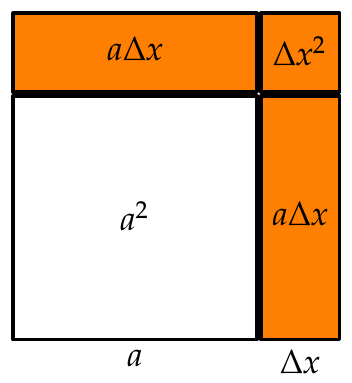
\includegraphics{img/derivadas/variacion_area_cuadrado.png}

}

\caption{Variación que experimenta el area de un cuadrado al variar el
lado}

\end{figure}

\end{example}

\hypertarget{interpretaciuxf3n-geomuxe9trica-de-la-tasa-de-variaciuxf3n-media}{%
\subsection{Interpretación geométrica de la tasa de variación
media}\label{interpretaciuxf3n-geomuxe9trica-de-la-tasa-de-variaciuxf3n-media}}

La tasa de variación media de \(f\) en el intervalo \([a,a+\Delta x]\)
es la pendiente de la recta \emph{secante} a \(f\) en los puntos
\((a,f(a))\) y \((a+\Delta x,f(a+\Delta x))\).

\begin{figure}

{\centering 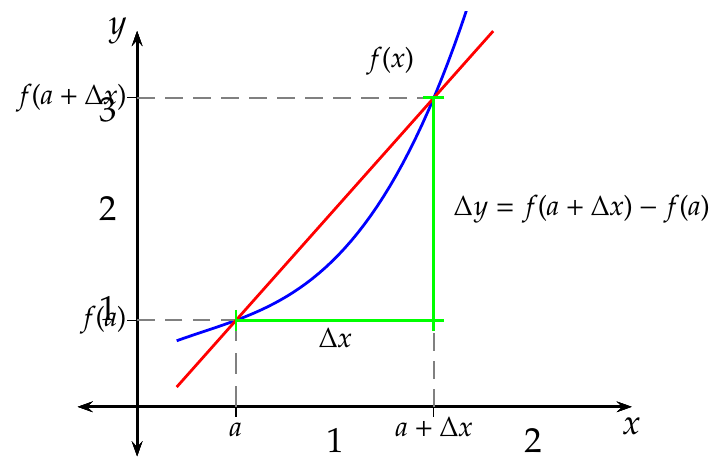
\includegraphics{img/derivadas/secante.png}

}

\caption{Gráfica de la recta secante a una función en dos puntos.}

\end{figure}

\hypertarget{tasa-de-variaciuxf3n-instantuxe1nea}{%
\subsection{Tasa de variación
instantánea}\label{tasa-de-variaciuxf3n-instantuxe1nea}}

En muchas ocasiones, es interesante estudiar la tasa de variación que
experimenta una función, no en intervalo, sino en un punto.

Conocer la tendencia de variación de una función en un instante puede
ayudarnos a predecir valores en instantes próximos.

\begin{definition}[Tasa de variación instantánea y
derivada]\protect\hypertarget{def-tasa-variacion-instantanea}{}\label{def-tasa-variacion-instantanea}

Dada una función \(y=f(x)\), se llama \emph{tasa de variación
instantánea} de \(f\) en un punto \(a\), al límite de la tasa de
variación media de \(f\) en el intervalo \([a,a+\Delta x]\), cuando
\(\Delta x\) tiende a 0, y se denota

\begin{align*}
\operatorname{TVI}(f,a) &= \lim_{\Delta x\rightarrow 0} \operatorname{TVM}(f,[a,a+\Delta x])=\lim_{\Delta x\rightarrow 0}\frac{\Delta y}{\Delta x} = \\
&= \lim_{\Delta x\rightarrow 0}\frac{f(a+\Delta x)-f(a)}{\Delta x}
\end{align*}

Cuando este límite existe, se dice que la función \(f\) es derivable en
el punto \(a\), y al valor del mismo se le llama derivada de \(f\) en
\(a\), y se nota como

\[
f'(a) \mbox{ o bien } \frac{df}{dx}(a)
\]

\end{definition}

\begin{example}[]\protect\hypertarget{exm-tasa-variacion-instantanea}{}\label{exm-tasa-variacion-instantanea}

Consideremos de nuevo la función \(y=x^2\) que mide el área de un
cuadrado de chapa metálica de lado \(x\).

Si en un determinado instante el lado del cuadrado es \(a\), y sometemos
la chapa a un proceso de calentamiento que aumenta el lado del cuadrado,
¿cuál es la tasa de variación instantánea del área del cuadrado en dicho
instante?

\begin{align*}
\operatorname{TVI}(f(a)) &=\lim_{\Delta x\rightarrow 0}\frac{\Delta y}{\Delta x}=\lim_{\Delta x\rightarrow 0}\frac{f(a+\Delta x)-f(a)}{\Delta x} =\\
&=\lim_{\Delta x\rightarrow 0}\frac{2a\Delta x+\Delta x^2}{\Delta x}=\lim_{\Delta x\rightarrow 0} 2a+\Delta x= 2a.
\end{align*}

Así pues, \(f'(a)=2a\), lo que indica que la tendencia de crecimiento el
área es del doble del valor del lado.

\end{example}

El signo de \(f'(a)\) indica la tendencia de crecimiento de \(f\) en el
punto \(a\):

\begin{itemize}
\tightlist
\item
  \(f'(a)>0\) indica que la tendencia es creciente.
\item
  \(f'(a)<0\) indica que la tendencia es decreciente.
\end{itemize}

\hypertarget{interpretaciuxf3n-geomuxe9trica-de-la-tasa-de-variaciuxf3n-instantuxe1nea}{%
\subsection{Interpretación geométrica de la tasa de variación
instantánea}\label{interpretaciuxf3n-geomuxe9trica-de-la-tasa-de-variaciuxf3n-instantuxe1nea}}

La tasa de variación instantánea de \(f\) en el punto \(a\) es la
pendiente de la recta \emph{tangente} a \(f\) en el punto \((a,f(a))\).

\begin{figure}

{\centering 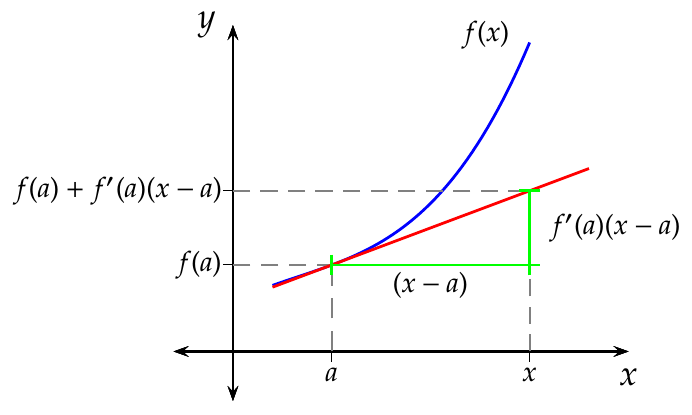
\includegraphics{img/derivadas/tangente.png}

}

\caption{Gráfica de la recta tangente a una función en un punto.}

\end{figure}

\begin{figure}

{\centering 

\href{https://www.geogebra.org/m/TX3ABH6F}{
\includegraphics{img/logos/logo-geogebra.png}}

}

\end{figure}

\hypertarget{diferenciabilidad}{%
\section{Diferenciabilidad}\label{diferenciabilidad}}

\begin{definition}[Función
derivable]\protect\hypertarget{def-funcion-diferenciable-derivada}{}\label{def-funcion-diferenciable-derivada}

Dado un intervalo \(I\subseteq\mathbb{R}\), una función
\(f:I\to\mathbb{R}\) y un punto \(a\in I\), se dice que \(f\) es
\emph{diferenciable} o \emph{derivable} en \(a\), si existe el límite

\[
\lim_{x\to a}\frac{f(x)-f(a)}{x-a}
\]

En tal caso, al valor del límite se le llama \emph{derivada} de \(f\) en
\(a\) y se denota \(f'(a)\).

Se dice que \(f\) es \emph{diferenciable} en el intervalo \(I\), si
\(f\) es diferenciable en todos los puntos de \(I\).

\end{definition}

\begin{tcolorbox}[enhanced jigsaw, colback=white, colbacktitle=quarto-callout-note-color!10!white, title=\textcolor{quarto-callout-note-color}{\faInfo}\hspace{0.5em}{Nota}, rightrule=.15mm, coltitle=black, arc=.35mm, opacityback=0, colframe=quarto-callout-note-color-frame, bottomtitle=1mm, titlerule=0mm, toptitle=1mm, bottomrule=.15mm, toprule=.15mm, breakable, opacitybacktitle=0.6, left=2mm, leftrule=.75mm]

Si en la definición anterior llamamos \(h=x-a\), resulta

\[
f'(a)=\lim_{x\to a}\frac{f(x)-f(a)}{x-a}=\lim_{h\to 0}\frac{f(a+h)-f(a)}{h},
\] que es otra definición equivalente de la derivada de \(f\) en \(a\).

\end{tcolorbox}

\begin{definition}[Función
derivada]\protect\hypertarget{def-funcion-derivada}{}\label{def-funcion-derivada}

Dado un intervalo \(I\subseteq\mathbb{R}\) y una función
\(f:I\to\mathbb{R}\), se define la \emph{función derivada} de \(f\), y
se denota \(f'\), a la función cuyo dominio es el conjunto de los puntos
de \(I\) donde \(f\) es diferenciable y el valor de \(f'\) es el valor
de la derivada en cada uno de esos puntos.

\end{definition}

\begin{tcolorbox}[enhanced jigsaw, colback=white, colbacktitle=quarto-callout-note-color!10!white, title=\textcolor{quarto-callout-note-color}{\faInfo}\hspace{0.5em}{Nota}, rightrule=.15mm, coltitle=black, arc=.35mm, opacityback=0, colframe=quarto-callout-note-color-frame, bottomtitle=1mm, titlerule=0mm, toptitle=1mm, bottomrule=.15mm, toprule=.15mm, breakable, opacitybacktitle=0.6, left=2mm, leftrule=.75mm]

La notación \(f'(a)\) para la derivada de \(f\) se debe a Lagrange, pero
también es común en Ciencias e Ingenierías utilizar la notación de
\(\frac{df}{dx}\) debida a Leibniz. En esta última notación \(df\) y
\(dx\) se conocen como \emph{diferenciales} de \(f\) y \(x\), y
representan variaciones infinitesimales de \(f\) y \(x\)
respectivamente.

\end{tcolorbox}

\begin{example}[]\protect\hypertarget{exm-derivada-1}{}\label{exm-derivada-1}

Sea \(f(x)=Id(x)=x\) la función identidad. Entonces, para cualquier
\(a\in\mathbb{R}\), se tiene que

\[
\lim_{x\to a}\frac{f(x)-f(a)}{x-a} = \lim_{x\to a}\frac{x-a}{x-a} = \lim_{x\to a}1 = 1.
\]

Por tanto, \(Id(x)\) es diferenciable en todo \(\mathbb{R}\) y
\(Id'(a)=a\).

Con la notación de Leibniz, el cálculo de la derivada es, si cabe, más
sencillo, pues se puede obtener algebraicamente,

\[
\frac{df}{dx} = \frac{dx}{dx} = 1.
\]

Sea ahora \(f(x)=x^2\). Entonces, para cualquier \(a\in\mathbb{R}\), se
tiene que

\[
\lim_{x\to a}\frac{f(x)-f(a)}{x-a} = \lim_{x\to a}\frac{x^2-a^2}{x-a} = \lim_{x\to a}\frac{(x-a)(x+a)}{x-a} = \lim_{x\to a}x+a = 2a.
\]

Por tanto, \(f(x)\) es diferenciable en todo \(\mathbb{R}\) y
\(f'(a)=2a\).

\end{example}

\begin{example}[]\protect\hypertarget{exm-derivada-2}{}\label{exm-derivada-2}

Sea la función \(f(x)=|x|\). Veamos si \(f\) es diferenciable en \(0\).
Para ello calculamos los límites laterales.

\begin{align*}
\lim_{x\to 0^-}\frac{f(x)-f(0)}{x-0} &= \lim_{x\to 0^-} \frac{|x|}{x} = \lim_{x\to 0^-} \frac{-x}{x} = -1,\\
\lim_{x\to 0^+}\frac{f(x)-f(0)}{x-0} &= \lim_{x\to 0^+} \frac{|x|}{x} = \lim_{x\to 0^+} \frac{x}{x} = 1,
\end{align*}

Por tanto, como los límites laterales no coinciden, \(f\) no es
diferenciable en \(0\).

\end{example}

\begin{definition}[Recta tangente a la gráfica de una
función]\protect\hypertarget{def-tangente-funcion}{}\label{def-tangente-funcion}

Dado un intervalo \(I\subseteq\mathbb{R}\), una función
\(f:I\to\mathbb{R}\) y un punto \(a\in I\), si \(f\) es diferenciable en
\(a\), se define la \emph{recta tangente} a la gráfica de \(f\) en \(a\)
como la recta que pasa por el punto \((a,f(a))\) con pendiente
\(f'(a)\), es decir, la recta con ecuación

\[
y=f(a)+f'(a)(x-a)
\]

\end{definition}

\begin{definition}[Recta normal a la gráfica de una
función]\protect\hypertarget{def-normal-funcion}{}\label{def-normal-funcion}

Dado un intervalo \(I\subseteq\mathbb{R}\), una función
\(f:I\to\mathbb{R}\) y un punto \(a\in I\), si \(f\) es diferenciable en
\(a\), se define la \emph{recta normal} a la gráfica de \(f\) en \(a\)
como la recta que pasa por el punto \((a,f(a))\) y es perpendicular a la
recta tangente a la gráfica de \(f\) en \(a\), es decir, la recta con
ecuación

\[
y=f(a)-\frac{1}{f'(a)}(x-a)
\]

\end{definition}

\begin{example}[]\protect\hypertarget{exm-tangente-normal-funcion}{}\label{exm-tangente-normal-funcion}

Dada la función \(y=f(x)=x^2\), la recta tangente a \(f\) en \(1\) es

\[
y = f(1)+f'(1)(x-1) = 1+2(x-1) = 2x-1,
\]

y la recta normal es

\[
y = f(1)-\frac{1}{f'(1)}(x-1) = 1-\frac{1}{2}(x-1) = \frac{-x}{2}+\frac{3}{2}.
\]

\end{example}

\begin{theorem}[]\protect\hypertarget{thm-diferenciabilidad-implica-continuidad}{}\label{thm-diferenciabilidad-implica-continuidad}

Dado un intervalo \(I\subseteq\mathbb{R}\), una función
\(f:I\to\mathbb{R}\) y un punto \(a\in I\), si \(f\) es diferenciable en
\(a\) entonces \(f\) es continua en \(a\).

\end{theorem}

\begin{tcolorbox}[enhanced jigsaw, colback=white, colbacktitle=quarto-callout-note-color!10!white, title=\textcolor{quarto-callout-note-color}{\faInfo}\hspace{0.5em}{Demostración}, rightrule=.15mm, coltitle=black, arc=.35mm, opacityback=0, colframe=quarto-callout-note-color-frame, bottomtitle=1mm, titlerule=0mm, toptitle=1mm, bottomrule=.15mm, toprule=.15mm, breakable, opacitybacktitle=0.6, left=2mm, leftrule=.75mm]

\begin{proof}

Sea \(x\in I\) y \(x\neq a\). Entonces

\[
\lim_{x\to a}f(x)-f(a) = \lim_{x\to a}\frac{f(x)-f(a)}{x-a}(x-a) = \lim_{x\to a}\frac{f(x)-f(a)}{x-a}\lim_{x\to a}x-a = f'(a)\cdot 0 = 0.
\]

Así pues,

\[
\lim_{x\to a}f(x)-f(a) = 0 \Rightarrow \lim_{x\to a}f(x)-\lim_{x\to a}f(a) = 0 \Rightarrow \lim_{x\to a}f(x)=\lim_{x\to a}f(a) =f(a),
\] y, por tanto, \(f\) es continua en \(a\).

\end{proof}

\end{tcolorbox}

\begin{tcolorbox}[enhanced jigsaw, colback=white, colbacktitle=quarto-callout-caution-color!10!white, title=\textcolor{quarto-callout-caution-color}{\faFire}\hspace{0.5em}{Precaución}, rightrule=.15mm, coltitle=black, arc=.35mm, opacityback=0, colframe=quarto-callout-caution-color-frame, bottomtitle=1mm, titlerule=0mm, toptitle=1mm, bottomrule=.15mm, toprule=.15mm, breakable, opacitybacktitle=0.6, left=2mm, leftrule=.75mm]

El recíproco de este teorema no es cierto, es decir, pueden existir
funciones continuas en un punto que no sean derivables en ese punto,
como por ejemplo la función \(f(x)=|x|\) que es continua en \(0\) pero,
como se ha visto, no es derivable en \(0\).

\end{tcolorbox}

\hypertarget{uxe1lgebra-de-derivadas}{%
\section{Álgebra de derivadas}\label{uxe1lgebra-de-derivadas}}

\begin{proposition}[]\protect\hypertarget{prp-algebra-derivadas}{}\label{prp-algebra-derivadas}

Dado un intervalo \(I\subseteq \mathbb{R}\) y dos funciones
\(f,g:I\to \mathbb{R}\), si \(f\) y \(g\) son diferenciables en
\(a\in I\), entonces

\begin{enumerate}
\def\labelenumi{\alph{enumi}.}
\item
  \(f+g\) es diferenciable en \(a\) y \((f+g)'(a)=f'(a)+g'(a)\).
\item
  \(f-g\) es diferenciable en \(a\) y \((f-g)'(a)=f'(a)-g'(a)\).
\item
  \(c\cdot f\) es diferenciable en \(a\) y
  \((c\cdot f)'(a) = c\cdot f'(a)\) \(\forall c \in \mathbb{R}\).
\item
  \(f\cdot g\) es diferenciable en \(a\) y
  \((f\cdot g)'(a) = f'(a)g(a)+f(a)g'(a)\).
\item
  Si \(g(c)\neq 0\), \(\frac{f}{g}\) es diferenciable en \(a\) y
  \(\left(\dfrac{f}{g}\right)'(a)=\dfrac{f'(a)g(a)-f(a)g'(a)}{g(a)^2}\).
\end{enumerate}

\end{proposition}

\begin{tcolorbox}[enhanced jigsaw, colback=white, colbacktitle=quarto-callout-note-color!10!white, title=\textcolor{quarto-callout-note-color}{\faInfo}\hspace{0.5em}{Demostración}, rightrule=.15mm, coltitle=black, arc=.35mm, opacityback=0, colframe=quarto-callout-note-color-frame, bottomtitle=1mm, titlerule=0mm, toptitle=1mm, bottomrule=.15mm, toprule=.15mm, breakable, opacitybacktitle=0.6, left=2mm, leftrule=.75mm]

\begin{proof}

Veamos la demostración de cada caso usando la definición de derivada.

\begin{enumerate}
\def\labelenumi{\alph{enumi}.}
\item
  Derivada de la suma de funciones. \begin{align*}
  (f+g)'(a) &=\lim_{x\to a}\frac{(f+g)(x)-(f+g)(a)}{x-a} = \lim_{x\to a}\frac{f(x)+g(x)-f(a)-g(a)}{x-a} \\
  &= \lim_{x\to a}\frac{f(x)-f(a)}{x-a}+\frac{g(x)-g(a)}{x-a} = \lim_{x\to a}\frac{f(x)-f(a)}{x-a}+\lim_{x\to a}\frac{g(x)-g(a)}{x-a}\\ 
  &= f'(a)+g'(a). 
  \end{align*}
\item
  Derivada de la resta de funciones. Se prueba del mismo modo que la
  suma.
\item
  Derivada del producto de una función por un escalar. \begin{align*}
  (c\cdot f)'(a) &=\lim_{x\to a}\frac{(c\cdot f)(x)-(c\cdot f)(a)}{x-a} = \lim_{x\to a}\frac{c\cdot f(a)-c\cdot f(a)}{x-a} \\
  &= \lim_{x\to a}\frac{c(f(x)-f(a))}{x-a} = c\lim_{x\to a}\frac{f(x)-f(a)}{x-a}= c\cdot f'(a). 
  \end{align*}
\item
  Derivada del producto de funciones. \begin{align*}
  (f\cdot g)'(a) &=\lim_{x\to a}\frac{(f\cdot g)(x)-(f\cdot g)(a)}{x-a} = \lim_{x\to a}\frac{f(x)\cdot g(x)-f(a)\cdot g(a)}{x-a} \\
  &= \lim_{x\to a}\frac{f(x)\cdot g(x)-f(a)\cdot g(x)+f(a)\cdot g(x)-f(a)\cdot g(a)}{x-a} \\ 
  &= \lim_{x\to a}\frac{(f(x)-f(a))\cdot g(x)+f(a)(g(x)-g(a))}{x-a} \\
  &= \lim_{x\to a}\frac{f(x)-f(a)}{x-a}\lim_{x\to a} g(x)+\lim_{x\to a}f(a)\lim_{x\to a}\frac{g(x)-g(a)}{x-a}  = f'(a)g(a)+f(a)g'(a).
  \end{align*}
\item
  Derivada del cociente de funciones. \begin{align*}
  (f\cdot g)'(a) &=\lim_{x\to a}\frac{(f/g)(x)-(f/g)(a)}{x-a} = \lim_{x\to a}\frac{f(x)/g(x)-f(a)/g(a)}{x-a} \\
  &= \lim_{x\to a}\frac{\frac{f(x)g(a)-f(a)g(x)}{g(x)g(a)}}{x-a} \\ 
  &= \lim_{x\to a}\frac{f(x)g(a)-f(a)g(x)}{(x-a)g(x)g(a)}\\ 
  &= \lim_{x\to a} \frac{f(x)g(a)-f(a)g(a)+f(a)g(a)-f(a)g(x)}{(x-a)g(x)g(a)} \\ 
  &= \lim_{x\to a} \frac{1}{g(x)g(a)}\left(\frac{f(x)-f(a)}{x-a}g(a) - f(a)\frac{g(x)-g(a)}{x-a}\right) \\ 
  &= \lim_{x\to a}\frac{1}{g(x)g(a)}\left(\lim_{x\to a}g(a)\lim_{x\to a}\frac{f(x)-f(a)}{x-a}-\lim_{x\to a}f(a)\lim_{x\to a}\frac{g(x)-g(a)}{x-a}\right) \\ 
  &= \frac{f'(a)g(a)-f(a)g'(a)}{g(a)^2},
  \end{align*} ya que \(g(a)\neq 0\) y como \(g\) es continua en \(a\)
  al ser derivable en \(a\), también se puede afirmar que existe un
  \(\delta>0\) tal que \(g(x)\neq 0\)
  \(\forall x \in (a-\delta, a+\delta)\cap I\), por lo que \[
  \lim_{x\to a}\frac{1}{g(x)g(a)}=\frac{1}{g(a)^2}.
  \]
\end{enumerate}

\end{proof}

\end{tcolorbox}

\begin{example}[]\protect\hypertarget{exm-algebra-derivadas}{}\label{exm-algebra-derivadas}

Veamos cuál es la función derivada de la función racional
\(f(x)=\dfrac{x^2-2x+1}{x}\).

\begin{align*}
f'(x) &= \frac{(x^2-2x+1)'x-(x^2-2x+1)x'}{x^2} = \frac{((x^2)'-(2x)'+1')x-(x^2-2x+1)}{x^2} = \\ 
&= \frac{(2x-2)x-(x^2-2x+1)}{x^2} =  \frac{2x^2-2x-x^2+2x-1}{x^2} = \frac{x^2-1}{x^2}  \forall x\neq 0.
\end{align*}

\end{example}

\hypertarget{regla-de-la-cadena}{%
\section{Regla de la cadena}\label{regla-de-la-cadena}}

El resultado anterior permite calcular la derivada de cualquier función
algebraica. A continuación se presenta otro importante resultado que nos
permitirá calcular la derivada de una composición de funciones.

\begin{theorem}[Regla de la
cadena]\protect\hypertarget{thm-regla-cadena}{}\label{thm-regla-cadena}

Dados dos intervalos \(I,J\subseteq \mathbb{R}\) y dos funciones
\(f:I\to \mathbb{R}\) y \(g:J\to\mathbb{R}\) tales que
\(f(I)\subseteq J\), si \(f\) es diferenciable en en \(a\) y \(g\) es
diferenciable en \(f(a)\), entonces \(g\circ f\) es diferenciable en
\(a\) y \[
(g\circ f)'(a) = g'(f(a))f'(a).
\]

\end{theorem}

\begin{tcolorbox}[enhanced jigsaw, colback=white, colbacktitle=quarto-callout-note-color!10!white, title=\textcolor{quarto-callout-note-color}{\faInfo}\hspace{0.5em}{Demostración}, rightrule=.15mm, coltitle=black, arc=.35mm, opacityback=0, colframe=quarto-callout-note-color-frame, bottomtitle=1mm, titlerule=0mm, toptitle=1mm, bottomrule=.15mm, toprule=.15mm, breakable, opacitybacktitle=0.6, left=2mm, leftrule=.75mm]

\begin{proof}

Sea

\[
h(y)=
\begin{cases}
\frac{g(y)-g(f(a))}{y-f(a)} & \mbox{si } y\in J \mbox{ y } y\neq f(a)\\
g'(f(a)) & \mbox{si } y=f(a)
\end{cases}
\]

Veamos que \(h\) es continua en \(f(a)\). Como \(g\) es diferenciable en
\(f(a)\), se tiene que
\(\lim_{x\to f(a)} \frac{g(x)-g(f(a))}{x-f(a)}=g'(f(a))\), de modo que
para cualquier \(\varepsilon>0\) existe \(\delta>0\) tal que si
\(x\in J\setminus \{f(a)\}\) y \(|x-f(a)|<\delta\), entonces
\(\left|\frac{g(x)-g(f(a))}{x-f(a)}-g'(f(a))\right|<\varepsilon\). Así
pues, si \(y\in J\), \(y\neq f(a)\) y \(|y-f(a)|<\delta\) entonces
\(|h(y)-g'(f(a))|<\varepsilon\), y si \(y=f(a)\), entonces
\(|y-f(a)|=0<\delta\) y
\(|h(y)-g'(f(a))|=|g'(f(a))-g'(f(a))|=0<\varepsilon\). Por consiguiente,
\(h\) es continua en \(f(a)\) y
\(\lim_{y\to f(a)}h(y)=h(f(a))=g'(f(a))\).

Por otro lado, de la definición de \(h\) se tiene que
\(g(y)-g(f(a))=h(y)(y-f(a))\) \(\forall y\in J\), de manera que si
\(x\in I\setminus\{a\}\) y \(y=f(x)\in J\) entonces

\begin{align*}
(g\circ f)'(a) &= \lim_{x\to a}\frac{g\circ f(x)-g\circ f(a)}{x-a} = \lim_{x\to a}\frac{g(f(x))-g(f(a))}{x-a} \\ 
& = \lim_{x\to a}\frac{h(f(x))(f(x)-f(a))}{x-a} = \lim_{x\to a}h(f(x))\lim_{x\to a}\frac{f(x)-f(a)}{x-a}\\ 
&= h(f(a))f'(a) = g'(f(a))f'(a).
\end{align*}

\begin{tcolorbox}[enhanced jigsaw, colback=white, colbacktitle=quarto-callout-note-color!10!white, title=\textcolor{quarto-callout-note-color}{\faInfo}\hspace{0.5em}{Nota}, rightrule=.15mm, coltitle=black, arc=.35mm, opacityback=0, colframe=quarto-callout-note-color-frame, bottomtitle=1mm, titlerule=0mm, toptitle=1mm, bottomrule=.15mm, toprule=.15mm, breakable, opacitybacktitle=0.6, left=2mm, leftrule=.75mm]

La demostración es mucho sencilla usando la notación diferencial de
Leibniz para la derivada. Si \(y=g(z)\) y \(z=f(x)\), entonces

\[
\frac{dy}{dx}=\frac{dy}{dz}\frac{dz}{dx}=g'(z)f'(x)=g'(f(x))f'(x).
\]

\end{tcolorbox}

\end{proof}

\end{tcolorbox}

\begin{example}[]\protect\hypertarget{exm-regla-cadena}{}\label{exm-regla-cadena}

Si \(g(x)=\operatorname{sen}(x)\) y \(f(x)=x^2\), entonces
\(g\circ f(x)=\operatorname{sen}(x^2)\) y, aplicando la regla de la
cadena, su derivada vale

\[
(g\circ f)'(x)=g'(f(x))f'(x) = \cos(g(x)) 2x = \cos(x^2)2x.
\]

Por otro lado, \(f\circ g(x)= (\sin(x))^2\) y, de nuevo aplicando la
regla de la cadena, su derivada vale

\[
(f\circ g)'(x)=f'(g(z))g'(z) = 2g(x)\cos(x) = 2\operatorname{sen}(x)\cos(x).
\]

\end{example}

\hypertarget{derivada-de-la-funciuxf3n-inversa}{%
\subsection{Derivada de la función
inversa}\label{derivada-de-la-funciuxf3n-inversa}}

La regla de la cadena nos permite calcular la derivada de la función
inversa de una función.

\begin{theorem}[Derivada de la función
inversa]\protect\hypertarget{thm-derivada-funcion-inversa}{}\label{thm-derivada-funcion-inversa}

Dado un intervalo \(I\subseteq \mathbb{R}\) y una función
\(f:I\to \mathbb{R}\) continua e inyectiva en \(I\), y sea \(J=f(I)\) y
\(f^{-1}:J\to\mathbb{R}\) la función inversa de \(f\). Si \(f\) es
diferenciable en \(a\in I\) y \(f'(a)\neq 0\), entonces \(f^{-1}\) es
diferenciable en \(f(a)\) y

\[
(f^{-1})'(f(a)) = \frac{1}{f'(a)}.
\]

\end{theorem}

\begin{tcolorbox}[enhanced jigsaw, colback=white, colbacktitle=quarto-callout-note-color!10!white, title=\textcolor{quarto-callout-note-color}{\faInfo}\hspace{0.5em}{Demostración}, rightrule=.15mm, coltitle=black, arc=.35mm, opacityback=0, colframe=quarto-callout-note-color-frame, bottomtitle=1mm, titlerule=0mm, toptitle=1mm, bottomrule=.15mm, toprule=.15mm, breakable, opacitybacktitle=0.6, left=2mm, leftrule=.75mm]

\begin{proof}

Como \(f\) es continua en \(I\), \(J=f(I)\) es un intervalo. Como además
\(f\) es inyectiva, necesariamente \(f\) es monótona. Sea la función
\(g(y)=\frac{y-f(a)}{f^{-1}(y)-a}\)
\(\forall y\in J\setminus \{f(a)\}\). \(g\) está bien definida pues
\(f^{-1}\) es inyectiva, y además, si \(y\neq f(a)\) entonces
\(f^{-1}(y) \neq f^{-1}(f(a))=a\), por lo que el denominador no se
anula. Veamos que \(\lim_{y\to f(a)}g(y)=f'(a)\).

Como \(f\) es diferenciable en \(a\), es decir,
\(f'(a)=\lim_{x\to a}\frac{f(x)-f(a)}{x-a}\), para cualquier
\(\varepsilon>0\) existe \(\delta'>0\) tal que si \(|x-a|<\delta'\)
entonces \(\left|\frac{f(x)-f(a)}{x-a}-f'(a)\right|<\varepsilon\).

Por otro lado, como \(f\) es continua en \(I\), \(f^{-1}\) es continua
en \(J\), y en particular en \(f(a)\), es decir,
\(\lim_{y\to f(a)}f^{-1}(y)=f^{-1}(f(a))=a\), de manera que para
cualquier \(\delta'>0\) existe \(\delta>0\) tal que si
\(y\in J\setminus\{f(a)\}\) y \(|y-f(a)|<\delta\) entonces
\(|f^{-1}(y)-a|<\delta'\), y por tanto,

\[
\begin{gathered}
\left|\frac{f(f^-1(y))-f(a)}{f^{-1}(y)-a}-f'(a)\right|<\varepsilon \Leftrightarrow \left|\frac{y-f(a)}{f^{-1}(y)-a}-f'(a)\right|<\varepsilon \\ 
\Leftrightarrow |g(y)-f'(a)|<\varepsilon \Rightarrow \lim_{y\to f(a)}g(y)=f'(a).
\end{gathered}
\]

Como además

\begin{align*}
\frac{f^{-1}(y)-f^{-1}(f(a))}{y-f(a)} &= \frac{f^{-1}(y)-a}{y-f(a)} \\ 
&= \frac{1}{\frac{y-f(a)}{f^{-1}(y)-a}} = \frac{1}{g(y)} \label{si $y\neq f(a)$}, 
\end{align*}

y como \(\lim_{y\to f(a)}\frac{1}{g(y)} = \frac{1}{f'(a)}\), finalmente
se tiene que

\[
(f^{-1})'(f(a)) = \lim_{y\to f(a)} \frac{f^{-1}(y)-f^{-1}(f(a))}{y-f(a)} = \lim_{y\to f(a)}\frac{1}{g(y)} = \frac{1}{f'(a)}.
\]

\begin{tcolorbox}[enhanced jigsaw, colback=white, colbacktitle=quarto-callout-note-color!10!white, title=\textcolor{quarto-callout-note-color}{\faInfo}\hspace{0.5em}{Nota}, rightrule=.15mm, coltitle=black, arc=.35mm, opacityback=0, colframe=quarto-callout-note-color-frame, bottomtitle=1mm, titlerule=0mm, toptitle=1mm, bottomrule=.15mm, toprule=.15mm, breakable, opacitybacktitle=0.6, left=2mm, leftrule=.75mm]

De nuevo, podemos realizar la demostración del teorema de manera más
sencilla utilizando la notación de diferencial de Leibniz.

\[
\frac{dx}{dy} = \frac{1}{dy/dx} = \frac{1}{f'(x)}
\]

\end{tcolorbox}

\begin{tcolorbox}[enhanced jigsaw, colback=white, colbacktitle=quarto-callout-caution-color!10!white, title=\textcolor{quarto-callout-caution-color}{\faFire}\hspace{0.5em}{Precaución}, rightrule=.15mm, coltitle=black, arc=.35mm, opacityback=0, colframe=quarto-callout-caution-color-frame, bottomtitle=1mm, titlerule=0mm, toptitle=1mm, bottomrule=.15mm, toprule=.15mm, breakable, opacitybacktitle=0.6, left=2mm, leftrule=.75mm]

Si en las condiciones del teorema anterior quitamos la condición
\(f'(a)\neq 0\), el resultado no es cierto y \(f^{-1}\) no es
diferenciable en \(f(a)\). Vamos a probarlo por reducción al absurdo.
Supongamos que \(f'(a)=0\), entonces, aplicando la regla de la cadena,
se tiene

\[
(f^{-1}\circ f)'(a) = (f^{-1})'(f(a))f'(a) = (f^{-1})'(f(a))0 = 0.
\]

Pero, por otro lado,
\((f^{-1}\circ f)'(a) = \operatorname{Id}'(a) = 1\), lo que supone una
contradicción, por lo que \(f^{-1}\) no puede ser derivable en \(f(a)\).

\end{tcolorbox}

\end{proof}

\end{tcolorbox}

\begin{corollary}[]\protect\hypertarget{cor-derivada-funcion-inversa}{}\label{cor-derivada-funcion-inversa}

Dado un intervalo \(I\subseteq\mathbb{R}\) y una función
\(f:I\to\mathbb{R}\) inyectiva en \(I\), y sea \(J=f(I)\) y
\(f^{-1}:J\to\mathbb{R}\) la función inversa de \(f\). Si \(f\) es
derivable en \(I\) y \(f'(x)\neq 0\) \(\forall x\in I\), entonces
\(f^{-1}\) es derivable en \(I\) y \(\forall y\in J\),

\[
(f^{-1})'(y) = \frac{1}{f'(f^{-1}(y))}
\]

\end{corollary}

\begin{tcolorbox}[enhanced jigsaw, colback=white, colbacktitle=quarto-callout-note-color!10!white, title=\textcolor{quarto-callout-note-color}{\faInfo}\hspace{0.5em}{Demostración}, rightrule=.15mm, coltitle=black, arc=.35mm, opacityback=0, colframe=quarto-callout-note-color-frame, bottomtitle=1mm, titlerule=0mm, toptitle=1mm, bottomrule=.15mm, toprule=.15mm, breakable, opacitybacktitle=0.6, left=2mm, leftrule=.75mm]

\begin{proof}

Si \(f\) es diferenciable en \(I\) entonces es continua en \(I\) y se
puede aplicar el teorema anterior.

\end{proof}

\end{tcolorbox}

\begin{example}[]\protect\hypertarget{exm-derivada-funcion-inversa}{}\label{exm-derivada-funcion-inversa}

La inversa de la función exponencial \(y=f(x)=e^x\) es el logaritmo
neperiano \(x=f^{-1}(y)=\ln y\), de modo que, aplicando el teorema
anterior, la función derivada del logaritmo es \[
\left(f^{-1}\right)'(y)=\frac{1}{f'(x)}=\frac{1}{e^x}=\frac{1}{e^{\ln y}}=\frac{1}{y}.
\]

\end{example}

\begin{example}[]\protect\hypertarget{exm-derivada-funcion-inversa-2}{}\label{exm-derivada-funcion-inversa-2}

Si \(n\in\mathbb{N}\) es par, la función \(f(x)=x^n\)
\(\forall x\in \mathbb{R}^+\) es inyectiva y derivable, con
\(f'(x)=nx^{n-1}>0\) \(\forall x\in\mathbb{R}^+\). Por tanto, la función
\(f^{-1}(y)=\sqrt[n]{y}\) es derivable en \(\mathbb{R}^+\) y
\(\forall y\in \mathbb{R}^+\),

\begin{align*}
(f^{-1})'(y) &= \frac{1}{f'(f^{-1}(y))} = \frac{1}{f'(\sqrt[n]{y})} = \frac{1}{n(\sqrt[n]{y})^{n-1}} \\ 
&= \frac{1}{n (y^{1/n})^{n-1}} = \frac{1}{ny^{1-\frac{1}{n}}} = \frac{1}{n}y^{\frac{1}{n}-1}.
\end{align*}

Por otro lado, si \(n\in\mathbb{N}\) es impar, la función \(f(x)=x^n\)
\(\forall x\in\mathbb{R}\) es inyectiva y derivable, con
\(f'(x)=nx^{n-1}\neq 0\) \(\forall x\neq 0\). Por tanto, la función
\(f^{-1}(y)=\sqrt[n]{y}\) es derivable en \(\mathbb{R}\setminus\{0\}\)
y, al igual que antes, \(\forall y\in \mathbb{R}^+\),

\[
(f^{-1})'(y) = \frac{1}{n}y^{\frac{1}{n}-1}.
\]

\end{example}

\hypertarget{derivadas-impluxedcitas}{%
\section{Derivadas implícitas}\label{derivadas-impluxedcitas}}

Hasta hora siempre hemos trabajado con funciones de la forma \(y=f(x)\)
donde la variable \(y\) depende de la variable \(x\) según la función
\(f(x)\). Esta representación se conoce como explícita, por que la
variable dependiente \(y\) aparece despejada en el lado izquierdo de la
igualdad. Sin embargo, como ya se vió en la
Definición~\ref{def-funcion}, una una función real de variable real es
una relación formada por pares \((x,y)\in \mathbb{R}\times\mathbb{R}\),
de modo que también se puede representar de manera intensiva mediante
una ecuación \(F(x,y)=0\), que cumplen los puntos de la función y solo
ellos.

\begin{example}[]\protect\hypertarget{exm-funcion-implicita}{}\label{exm-funcion-implicita}

La función \(y=x^2\) también se puede expresar implícitamente mediante
la ecuación \(y-x^2=0\).

\end{example}

\begin{tcolorbox}[enhanced jigsaw, colback=white, colbacktitle=quarto-callout-caution-color!10!white, title=\textcolor{quarto-callout-caution-color}{\faFire}\hspace{0.5em}{Precaución}, rightrule=.15mm, coltitle=black, arc=.35mm, opacityback=0, colframe=quarto-callout-caution-color-frame, bottomtitle=1mm, titlerule=0mm, toptitle=1mm, bottomrule=.15mm, toprule=.15mm, breakable, opacitybacktitle=0.6, left=2mm, leftrule=.75mm]

El problema de la representación implícita es que no toda ecuación en
\(x\) e \(y\) define una función. Por ejemplo, la ecuación \(y^2-x=0\)
no define una función, ya que si se despeja \(y\) de la ecuación se
obtiene \(y=\pm\sqrt{x}\), que no es una función ya que para cualquier
valor de \(x>0\), \(y\) puede tomar dos valores, lo cual no está
permitido en una función.

\end{tcolorbox}

Dada una ecuación \(F(x,y)=0\), que define implícitamente \(y\) como
función de \(x\), si \(y\) es derivable en un punto \((x_0, y_0)\), se
puede calcular la derivada mediante el siguiente procedimiento:

\begin{enumerate}
\def\labelenumi{\arabic{enumi}.}
\item
  Calcular la derivada de las expresiones de ambos lados de la ecuación.
  \(F'(x,y)=0\). En el cálculo de estas derivadas hay que tener en
  cuenta que \(y\) es una función que depende de \(x\) y aplicar la
  regla de la cadena para derivarla.
\item
  Reescribir la ecuación de manera que los términos donde aparezca
  \(y'\) queden a un lado de la ecuación y el resto al otro.
\item
  Sacar \(y'\) factor común en el lado de la ecuación donde aparezca.
\item
  Resolver la ecuación para \(y'\).
\item
  Sustituir \(x=x_0\), \(y=y_0\).
\end{enumerate}

\begin{example}[]\protect\hypertarget{exm-derivada-implicita}{}\label{exm-derivada-implicita}

Dada la ecuación \(e^y-x^2=0\) que define a \(y\) como función implícita
de \(x\), veamos cómo calcular su derivada en el punto \((1,0)\)
implícitamente

\begin{align*}
(e^y-x^2)' = 0' &\Rightarrow e^yy'-2x = 0 \Rightarrow e^yy' = 2x \Rightarrow y' = \frac{2x}{e^y}.
\end{align*}

Sustituyendo \(x=1\) e \(y=0\), se tiene
\(y'(1) = \frac{2\cdot 1}{e^0} = 2\).

En este caso, es posible obtener la representación explícita de la
función, ya que
\(e^y-x^2=0 \Rightarrow e^y=x^2 \Rightarrow y=\ln(x^2) = 2\ln(x)\). Si
calculamos su derivada explícitamente, se tiene \(y'=\frac{2}{x}\), y
para \(x=1\) se tiene \(y'(1) = \frac{2}{1}=2\), que coincide con el
resultado anterior.

\end{example}

Aún cuando la ecuación \(F(x,y)=0\) no defina implícitamente a \(y\)
como función de \(x\), es posible utiliza el procedimiento anterior para
estudiar la tasa de variación instantánea de \(y\) con respecto a \(x\)
en un punto \((x_0, y_0)\) que cumpla la ecuación.

\begin{example}[]\protect\hypertarget{exm-derivada-implicita-2}{}\label{exm-derivada-implicita-2}

La ecuación \(x^2-xy+y^2=1\) no define a \(y\) como función explícita de
\(x\), ya que para \(x=0\) se obtienen dos posibles valores de \(y\),
\(0^2-0\cdot y+y^2=1 \Rightarrow y^2=1 \Rightarrow y=\pm 1\). No
obstante, en el punto \((0,1)\), se puede calcular la tasa de variación
instantánea de \(y\) con respecto a \(x\),

\[
\begin{gathered}
(x^2-xy+y^2)' = 1' \Rightarrow (x^2)'-(xy)'+(y^2)' = 0 \\ \Rightarrow 2x -(1\cdot y+xy')+2yy' = 0 \Rightarrow 2x-y-xy'+2yy'=0 \\ 
\Rightarrow y'(-x+2y)=-2x+y \Rightarrow y'=\frac{-2x+y}{-x+2y},
\end{gathered}
\]

y sustituyendo \(x=0\), \(y=1\) se tiene
\(y'(0)=\frac{-2\cdot 0+1}{-0+2\cdot 1} = \frac{1}{2}\).

Si dibujamos la gráfica de los puntos que cumplen la ecuación, se puede
comprobar que la recta tangente a la gráfica en el punto \((0,1)\) tiene
pendiente \(1/2\).

\begin{figure}

{\centering 

\begin{tikzpicture}[x=5cm,y=5cm]
\pgfplotsset{grid style={dashed,mygray, line width=0.1pt}}
\tikzset{
outer dot/.style = {scale=2.5*sqrt(\pgflinewidth)},
  inner dot/.style = {scale=sqrt(\pgflinewidth),#1},inner dot/.default={white},
  point/.style={insert path={ node[outer dot]{.} node[inner dot=#1]
{.}}}
}
\begin{axis}[
grid=major,
domain=-3:3,
%restrict y to domain=-5:5,
xmin=-2, xmax=2,
ymin=-2, ymax=2,
samples=100,
x=1cm, y=1cm,
axis lines=middle,
%no markers,
color=myblack,
legend style={fill=none, color=myblack, at={(0.5,1.04)},anchor=south, legend columns=2, legend cell align=left}
]
\coordinate (A) at (axis cs: {0}, {0});
\coordinate (B) at (axis cs: {0}, {1});
\draw [rotate around={45:(0,0)},line width=1pt, myblue] (A) ellipse (1.4142135623730951cm and 0.816496580927726cm);
\addplot[domain=0:0.1] {x+10};
\addplot[domain=-2:2, line width=1pt, myred] {1+x/2};
\draw[very thick] (B) --  node[point]{} (B);
\legend{$x^2-xy+y^2=1$, $y=x+\frac{1}{2}$};
\end{axis}
\end{tikzpicture}

}

\caption{Recta tangente a la curva implícita \(x^2-xy+y^2=1\) en el
punto \((0,1)\).}

\end{figure}

\end{example}

\hypertarget{teorema-del-valor-medio-y-aplicaciones}{%
\section{Teorema del valor medio y
aplicaciones}\label{teorema-del-valor-medio-y-aplicaciones}}

\begin{theorem}[Extremo
interior]\protect\hypertarget{thm-extremo-interior}{}\label{thm-extremo-interior}

Dado un intervalo \(I\subseteq \mathbb{R}\) y una función
\(f:I\to\mathbb{R}\) con un extremo relativo en un punto interior
\(a\in I\), si \(f\) es diferenciable en \(a\), entonces \(f'(a)=0\).

\end{theorem}

\begin{tcolorbox}[enhanced jigsaw, colback=white, colbacktitle=quarto-callout-note-color!10!white, title=\textcolor{quarto-callout-note-color}{\faInfo}\hspace{0.5em}{Demostración}, rightrule=.15mm, coltitle=black, arc=.35mm, opacityback=0, colframe=quarto-callout-note-color-frame, bottomtitle=1mm, titlerule=0mm, toptitle=1mm, bottomrule=.15mm, toprule=.15mm, breakable, opacitybacktitle=0.6, left=2mm, leftrule=.75mm]

\begin{proof}

Supongamos que \(f\) tiene un máximo relativo en \(a\in I\). Por ser
\(a\) un punto interior de \(I\), existe un \(\delta>0\) tal que el
entorno \((a-\delta, a+\delta)\subset I\) y \(f(x)<f(a)\)
\(\forall x\in (a-\delta,a+\delta)\).

Supongamos ahora que \(f'(a)>0\). Como
\(f'(a)=\lim_{x\to a}\frac{f(x)-f(a)}{x-a}\), existe un
\(0<\delta'<\delta\) tal que \(\frac{f(x)-f(a)}{x-a}>0\)
\(\forall x\in (a-\delta',a+\delta')\setminus\{a\}\). Por tanto, si
\(x\in (a,a+\delta')\), \(f(x)-f(a)>0\) de donde se deduce que
\(f(x)>f(a)\) lo que contradice que \(f\) tenga un máximo relativo en
\(a\). Así que no puede ser \(f'(c)>0\).

Del mismo modo se puede probar que no puede ser \(f'(a)<0\). Por lo que
necesariamente tiene que ser \(f'(a)=0\).

Si \(f\) tiene un mínimo relativo en \(a\), la demostración es análoga.

\end{proof}

\end{tcolorbox}

\begin{tcolorbox}[enhanced jigsaw, colback=white, colbacktitle=quarto-callout-caution-color!10!white, title=\textcolor{quarto-callout-caution-color}{\faFire}\hspace{0.5em}{Precaución}, rightrule=.15mm, coltitle=black, arc=.35mm, opacityback=0, colframe=quarto-callout-caution-color-frame, bottomtitle=1mm, titlerule=0mm, toptitle=1mm, bottomrule=.15mm, toprule=.15mm, breakable, opacitybacktitle=0.6, left=2mm, leftrule=.75mm]

El resultado anterior no es cierto si el punto \(a\) no es interior de
\(I\). Para verlo, basta considerar \(f(x)=x\) \(\forall x\in[0,1]\). Se
observa que \(f\) tiene un máximo relativo en \(1\), pero
\(f'(1)\neq 0\).

\end{tcolorbox}

\begin{corollary}[]\protect\hypertarget{cor-extremo-interior}{}\label{cor-extremo-interior}

Dado un intervalo \(I\subseteq \mathbb{R}\) y una función
\(f:I\to\mathbb{R}\) con un extremo relativo en un punto \(a\in I\),
entonces \(f'(a)\) no existe o \(f'(a)=0\).

\end{corollary}

\begin{example}[]\protect\hypertarget{exm-extremo-interior-valor-absoluto}{}\label{exm-extremo-interior-valor-absoluto}

La función \(f(x)=|x|\) tiene un mínimo relativo en \(0\) que es un
punto interior de \(\mathbb{R}\). Sin embargo, \(f'(0)\) no existe.

\end{example}

\begin{definition}[Punto
crítico]\protect\hypertarget{def-punto-critico}{}\label{def-punto-critico}

Dado un intervalo \(I\subseteq\mathbb{R}\) y una función
\(f:I\to\mathbb{R}\), se dice que \(a\) es un \emph{punto crítico} o
\emph{punto singular} de \(f\), si \(f'(a)=0\).

\end{definition}

Gráficamente, los puntos críticos son puntos donde la tangente a la
gráfica de la función es horizontal.

Como veremos más adelante, los puntos críticos juegan un papel clave en
la determinación de los extremos relativos de una función.

\begin{theorem}[Rolle]\protect\hypertarget{thm-rolle}{}\label{thm-rolle}

Dada una función \(f:[a,b]\to\mathbb{R}\) continua en \([a,b]\) y
diferenciable en \((a,b)\), si \(f(a)=f(b)\), entonces \(f\) tiene al
menos un punto crítico en \((a,b)\), es decir, existe \(c\in(a,b)\) tal
que \(f'(c)=0\).

\end{theorem}

\begin{tcolorbox}[enhanced jigsaw, colback=white, colbacktitle=quarto-callout-note-color!10!white, title=\textcolor{quarto-callout-note-color}{\faInfo}\hspace{0.5em}{Demostración}, rightrule=.15mm, coltitle=black, arc=.35mm, opacityback=0, colframe=quarto-callout-note-color-frame, bottomtitle=1mm, titlerule=0mm, toptitle=1mm, bottomrule=.15mm, toprule=.15mm, breakable, opacitybacktitle=0.6, left=2mm, leftrule=.75mm]

\begin{proof}

Como \(f\) es continua en \([a,b]\), por el
Teorema~\ref{thm-extremos-funcion-continua-intervalo-cerrado} \(f\)
alcanza el máximo y el mínimo en \([a,b]\). Si existe \(c\in (a,b)\) tal
que \(f\) alcanza el máximo o el mínimo en \(c\), por el teorema
anterior se tiene \(f'(c)=0\). En caso contrario, si no existe
\(c\in(a,b)\) tal que \(f\) alcanza el máximo o el mínimo en \(c\),
entonces \(f\) alcanza el máximo o el mínimo en los extremos del
intervalo, pero como \(f(a)=f(b)\), se deduce que que \(f\) es constante
en \([a,b]\) y, por tanto, \(f'(x)=0\) \(\forall x\in (a,b)\).

\end{proof}

\end{tcolorbox}

\begin{theorem}[Valor
medio]\protect\hypertarget{thm-valor-medio}{}\label{thm-valor-medio}

Dada una función \(f:[a,b]\to\mathbb{R}\) continua en \([a,b]\) y
diferenciable en \((a,b)\), entonces existe \(c\in (a,b)\) tal que

\[
f'(c) = \frac{f(b)-f(a)}{b-a}.
\]

\end{theorem}

\begin{tcolorbox}[enhanced jigsaw, colback=white, colbacktitle=quarto-callout-note-color!10!white, title=\textcolor{quarto-callout-note-color}{\faInfo}\hspace{0.5em}{Demostración}, rightrule=.15mm, coltitle=black, arc=.35mm, opacityback=0, colframe=quarto-callout-note-color-frame, bottomtitle=1mm, titlerule=0mm, toptitle=1mm, bottomrule=.15mm, toprule=.15mm, breakable, opacitybacktitle=0.6, left=2mm, leftrule=.75mm]

\begin{proof}

Sea \(g(x)\) la recta secante a \(f\) en los puntos \((a,f(a))\) y
\((b,f(b))\). Entonces
\(g(x)=f(a)+\operatorname{TVM}(f,[a,b])(x-a) = f(a)+\frac{f(b)-f(a)}{b-a}(x-a)\).
Si tomamos la función que mide la distancia entre \(f\) y \(g\), es
decir, \(\forall x\in[a,b]\)

\[
h(x)=f(x)-g(x)= f(x)-f(a)+\frac{f(b)-f(a)}{b-a}(x-a),
\]

\(h\) es continua en \([a,b]\) por ser la diferencia de dos funciones
continuas en ese intervalo, también es derivable en \((a,b)\) al ser
\(f\) y \(g\) derivables en el intervalo. Además

\begin{align*}
h(a) &= f(a) - f(a)+\frac{f(b)-f(a)}{b-a}(a-a) = 0,\\
h(b) &= f(a) - f(b)+\frac{f(b)-f(a)}{b-a}(b-a) = 0.\\
\end{align*}

Por tanto, aplicando el teorema de Rolle, existe \(c\in(a,b)\) tal que
\(f'(c)=0\). Como

\[
h'(x) = f'(x) - \frac{f(b)-f(a)}{b-a} \ \forall x\in (a,b),
\]

en particular se tiene

\[
h'(c) = f'(c) - \frac{f(b)-f(a)}{b-a} = 0 \Rightarrow f'(c) = \frac{f(b)-f(a)}{b-a}.
\]

\end{proof}

\end{tcolorbox}

\hypertarget{estudio-del-crecimiento-de-una-funciuxf3n}{%
\subsection{Estudio del crecimiento de una
función}\label{estudio-del-crecimiento-de-una-funciuxf3n}}

La principal aplicación de la derivada es el estudio del crecimiento de
una función mediante el signo de la derivada.

\begin{theorem}[Signo de la
derivada]\protect\hypertarget{thm-crecimiento-signo-derivada}{}\label{thm-crecimiento-signo-derivada}

Dado un intervalo \(I\subseteq\mathbb{R}\) y una función
\(f:I\to\mathbb{R}\) diferenciable en \(I\), entonces:

\begin{enumerate}
\def\labelenumi{\alph{enumi}.}
\tightlist
\item
  \(f\) es creciente en \(I\) si y sólo si \(f'(x)\geq 0\)
  \(\forall x\in I\).
\item
  \(f\) es decreciente en \(I\) si y sólo si \(f'(x)\leq 0\)
  \(\forall x\in I\).
\end{enumerate}

\end{theorem}

\begin{tcolorbox}[enhanced jigsaw, colback=white, colbacktitle=quarto-callout-note-color!10!white, title=\textcolor{quarto-callout-note-color}{\faInfo}\hspace{0.5em}{Demostración}, rightrule=.15mm, coltitle=black, arc=.35mm, opacityback=0, colframe=quarto-callout-note-color-frame, bottomtitle=1mm, titlerule=0mm, toptitle=1mm, bottomrule=.15mm, toprule=.15mm, breakable, opacitybacktitle=0.6, left=2mm, leftrule=.75mm]

\begin{proof}

Probaremos solo el primer apartado, ya que el segundo se prueba de forma
análoga.

Supongamos que \(f\) es creciente en \(I\) y sea \(a\in I\). Si
\(x\in I\) y \(x>a\), por ser \(f\) creciente, \(f(x)>f(a)\), por lo que
\(\frac{f(x)-f(a)}{x-a}\geq 0\). Y si \(x<a\), \(f(x)<f(a)\), por lo que
también se tiene \(\frac{f(x)-f(a)}{x-a}\geq 0\). Así pues,
\(f'(a)=\lim_{x\to a}\frac{f(x)-f(a)}{x-a}\geq 0\).

Para ver el otro sentido de la implicación, supongamos que
\(f'(x)\geq 0\) \(\forall x\in I\), y sean \(a,b\in I\) con \(a<b\).
Aplicando el teorema del valor medio a \(f\) en el intervalo \([a,b]\),
se tiene que existe \(c\in(a,b)\) tal que
\(f'(c)= \frac{f(b)-f(a)}{b-a}\geq 0\), y como \(b-a>0\), se tiene que
\(f(b)-f(a)>0\) por lo que \(f(b)>f(a)\) y, por tanto, \(f\) es
creciente en \(I\).

\end{proof}

\end{tcolorbox}

\begin{example}[]\protect\hypertarget{exm-crecimiento}{}\label{exm-crecimiento}

La función \(f(x)=x^3\) es creciente en todo \(\mathbb{R}\) ya que
\(\forall x\in \mathbb{R}\ f'(x)\geq 0\).

\end{example}

\begin{tcolorbox}[enhanced jigsaw, colback=white, colbacktitle=quarto-callout-warning-color!10!white, title=\textcolor{quarto-callout-warning-color}{\faExclamationTriangle}\hspace{0.5em}{Advertencia}, rightrule=.15mm, coltitle=black, arc=.35mm, opacityback=0, colframe=quarto-callout-warning-color-frame, bottomtitle=1mm, titlerule=0mm, toptitle=1mm, bottomrule=.15mm, toprule=.15mm, breakable, opacitybacktitle=0.6, left=2mm, leftrule=.75mm]

Una función puede ser creciente o decreciente en un intervalo y no tener
derivada.

\end{tcolorbox}

\begin{example}[]\protect\hypertarget{exm-crecimiento-2}{}\label{exm-crecimiento-2}

Consideremos la función \(f(x)=x^4-2x^2+1\). Su derivada
\(f'(x)=4x^3-4x\) está definida en todo \(\mathbb{R}\) y es continua.

\begin{figure}

{\centering 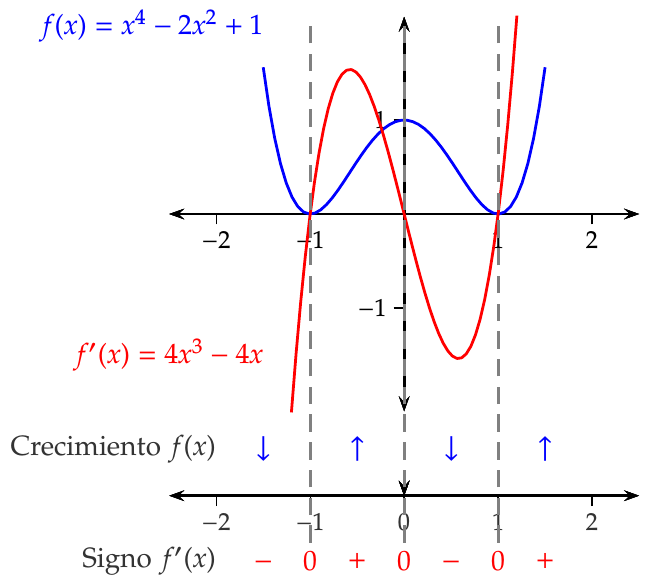
\includegraphics{img/derivadas/crecimiento.png}

}

\caption{Estudio del crecimiento de una función.}

\end{figure}

\end{example}

\hypertarget{determinaciuxf3n-de-los-extremos-relativos-de-una-funciuxf3n}{%
\subsection{Determinación de los extremos relativos de una
función}\label{determinaciuxf3n-de-los-extremos-relativos-de-una-funciuxf3n}}

Como consecuencia del resultado anterior, la derivada también sirve para
determinar los extremos relativos de una función.

\begin{theorem}[Criterio de la primera
derivada]\protect\hypertarget{thm-extremos-relativos}{}\label{thm-extremos-relativos}

Sea una función \(f:[a,b]\to\mathbb{R}\) continua en \([a,b]\) y
derivable en \((a,c)\cup (c,b)\) para un punto \(c\in(a,b)\).

\begin{enumerate}
\def\labelenumi{\alph{enumi}.}
\tightlist
\item
  Si existe un \(\delta>0\) tal que
  \((c-\delta, c+\delta)\subseteq[a,b]\) y \(f'(x)\geq 0\) y
  \(\forall x\in(c-\delta,c)\) y \(f'(x)\leq 0\)
  \(\forall x\in(c,c+\delta)\), entonces \(f\) tiene un \emph{máximo
  relativo} en \(c\).
\item
  Si existe un \(\delta>0\) tal que
  \((c-\delta, c+\delta)\subseteq[a,b]\) y \(f'(x)\leq 0\) y
  \(\forall x\in(c-\delta,c)\) y \(f'(x)\geq 0\)
  \(\forall x\in(c,c+\delta)\), entonces \(f\) tiene un \emph{mínimo
  relativo} en \(c\).
\end{enumerate}

\end{theorem}

\begin{tcolorbox}[enhanced jigsaw, colback=white, colbacktitle=quarto-callout-note-color!10!white, title=\textcolor{quarto-callout-note-color}{\faInfo}\hspace{0.5em}{Demostración}, rightrule=.15mm, coltitle=black, arc=.35mm, opacityback=0, colframe=quarto-callout-note-color-frame, bottomtitle=1mm, titlerule=0mm, toptitle=1mm, bottomrule=.15mm, toprule=.15mm, breakable, opacitybacktitle=0.6, left=2mm, leftrule=.75mm]

\begin{proof}

Demostraremos solo el caso de un máximo, ya que el otro caso es análogo.
Para ver que \(f\) tiene un máximo local en \(c\) basta con probar que
si \(x\in(c-\delta,c+\delta)\) entonces \(f(x)\leq f(c)\).

Si \(x\in(c-\delta,c)\) entonces \(f'(x)\geq 0\). Aplicando el teorema
del valor medio a \(f\) en el intervalo \([x,c]\) se tiene que existe
\(u\in(x,c)\) tal que \(f'(u)=\frac{f(c)-f(x)}{c-x}\geq 0\), y como
\(c-x>0\) se concluye que \(f(c)-f(x)\geq 0\), y por tanto,
\(f(x)\leq f(c)\).

Y si Si \(x\in(c, c+\delta)\) entonces \(f'(x)\leq 0\). Aplicando de
nuevo el teorema del valor medio a \(f\) en el intervalo \([c,x]\) se
tiene que existe \(v\in(c,x)\) tal que
\(f'(v)=\frac{f(x)-f(c)}{x-c}\leq 0\), y como \(x-c>0\) se concluye que
\(f(x)-f(c)\leq 0\), y por tanto, \(f(x)\leq f(c)\).

\end{proof}

\end{tcolorbox}

\begin{example}[]\protect\hypertarget{exm-extremos-relativos}{}\label{exm-extremos-relativos}

Consideremos de nuevo la función \(f(x)=x^4-2x^2+1\). Su derivada
\(f'(x)=4x^3-4x\) está definida en todo \(\mathbb{R}\) y es continua.

\begin{figure}

{\centering 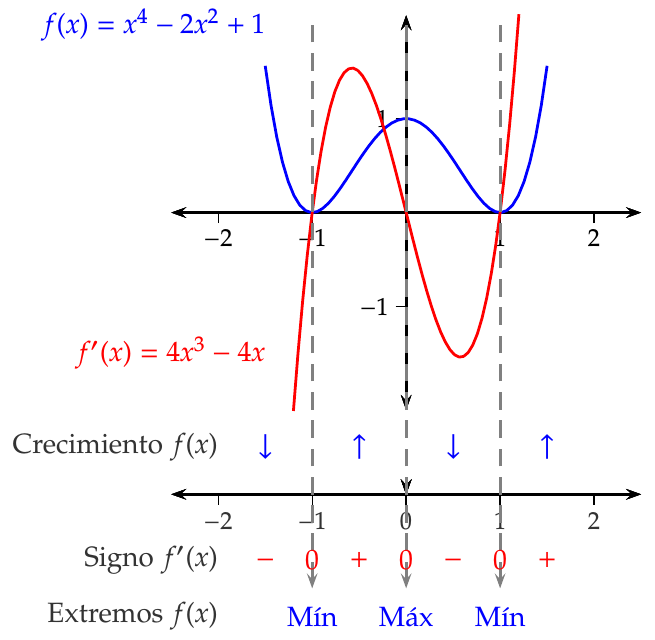
\includegraphics{img/derivadas/extremos.png}

}

\caption{Estudio de los extremos de una función}

\end{figure}

\end{example}

\begin{tcolorbox}[enhanced jigsaw, colback=white, colbacktitle=quarto-callout-caution-color!10!white, title=\textcolor{quarto-callout-caution-color}{\faFire}\hspace{0.5em}{Precaución}, rightrule=.15mm, coltitle=black, arc=.35mm, opacityback=0, colframe=quarto-callout-caution-color-frame, bottomtitle=1mm, titlerule=0mm, toptitle=1mm, bottomrule=.15mm, toprule=.15mm, breakable, opacitybacktitle=0.6, left=2mm, leftrule=.75mm]

El recíproco de las implicaciones del teorema anterior no tiene por qué
ser cierto. Por ejemplo, la función

\[
f(x)=
\begin{cases}
2x^4+x^4\operatorname{sen}\left(\frac{1}{x}\right) & \mbox{si } x\neq 0,\\
0 & \mbox{si } x=0.
\end{cases}
\]

tiene un mínimo relativo y absoluto en \(x=0\), pero su derivada toma
valores positivos y negativos en cualquier entorno de \(0\).

\end{tcolorbox}

\begin{theorem}[Darboux]\protect\hypertarget{thm-darboux}{}\label{thm-darboux}

Dada una función \(f:[a,b]\to\mathbb{R}\), si \(f\) es diferenciable en
\([a,b]\) y \(f'(a)<k<f'(b)\), entonces existe \(c\in(a,b)\) tal que
\(f'(c)=k\).

\end{theorem}

\begin{tcolorbox}[enhanced jigsaw, colback=white, colbacktitle=quarto-callout-note-color!10!white, title=\textcolor{quarto-callout-note-color}{\faInfo}\hspace{0.5em}{Demostración}, rightrule=.15mm, coltitle=black, arc=.35mm, opacityback=0, colframe=quarto-callout-note-color-frame, bottomtitle=1mm, titlerule=0mm, toptitle=1mm, bottomrule=.15mm, toprule=.15mm, breakable, opacitybacktitle=0.6, left=2mm, leftrule=.75mm]

\begin{proof}

Definimos \(g(x)=k(x-a)-f(x)\) \(\forall x\in[a,b]\). \(g\) es
diferenciable en \([a,b]\) al serlo \(f\) y \(g'(x)=k-f'(x)\)
\(\forall x\in[a,b]\). Por tanto, \(g\) es continua en \([a,b]\), y
entonces tiene un máximo y un mínimo relativos en \([a,b]\).

Por otro lado, \(g'(a)=k-f'(a)>0\), de manera que \(g\) no tiene un
máximo relativo en \(a\), y \(g'(b)=k-f'(b)<0\), de manera que \(g\)
tampoco tiene un máximo relativo en \(b\). Por tanto, \(g\) alcanza el
máximo relativo en un punto \(c\in (a,b)\), y por el teorema del extremo
interior, \(g'(c)=0\), de donde se deduce que \(k-f(c)=0\), y
\(f'(c)=k\).

\end{proof}

\end{tcolorbox}

\hypertarget{determinaciuxf3n-de-los-extremos-absolutos-de-una-funciuxf3n}{%
\subsection{Determinación de los extremos absolutos de una
función}\label{determinaciuxf3n-de-los-extremos-absolutos-de-una-funciuxf3n}}

Ya se vió, por el
Teorema~\ref{thm-extremos-funcion-continua-intervalo-cerrado}, que una
función continua en un intervalo cerrado \([a,b]\) alcanza el máximo y
el mínimo absolutos en ese intervalo. Así pues, para encontrar los
extremos absolutos de una función \(f\) derivable en \([a,b]\), basta
con seguir el siguiente procedimiento:

\begin{enumerate}
\def\labelenumi{\arabic{enumi}.}
\tightlist
\item
  Calcular los puntos críticos de \(f\).
\item
  Calcular los valores de \(f\) en los puntos críticos.
\item
  Calcular el valor de \(f\) en los extremos del intervalo, \(a\) y
  \(b\).
\item
  El máximo absoluto será el mayor de los valores obtenidos en los pasos
  2 y 3, y el mínimo absoluto será el menor de los valores obtenidos en
  esos mismos pasos.
\end{enumerate}

\begin{example}[]\protect\hypertarget{exm-extremos-absolutos}{}\label{exm-extremos-absolutos}

Veamos cuáles son los extremos absolutos de la función
\(f(x)=x^4-2x^2+1\) en el intervalo \([0,2]\). Seguiremos el
procedimiento anterior para la determinación de los extremos absolutos.

\begin{enumerate}
\def\labelenumi{\arabic{enumi}.}
\item
  En el Ejemplo~\ref{exm-extremos-relativos} se vió que \(f\) tenía tres
  puntos críticos en \(-1\), \(0\) y \(1\). El punto crítico en \(-1\)
  se puede descartar al no pertenecer al intervalo \([0,2]\).
\item
  El valor de la función en los puntos críticos del intervalo \([0,2]\)
  son \(f(0)=1\) y \(f(1)=0\).
\item
  El valor de la función en los extremos del intervalo \([0,2]\) es
  \(f(0)=1\) y \(f(2)=9\).
\item
  El máximo absoluto de \(f\) en \([a,b]\) es
  \(\max\{f(0),f(1),f(2)\}=\max\{1,0,9\}=9\) y el mínimo absoluto es
  \(\min\{f(0),f(1),f(2)\}=\max\{1,0,9\}=0\).
\end{enumerate}

\end{example}

\hypertarget{otras-aplicaciones-del-teorema-del-valor-medio}{%
\subsection{Otras aplicaciones del teorema del valor
medio}\label{otras-aplicaciones-del-teorema-del-valor-medio}}

Además del estudio del crecimiento de una función y de la determinación
de sus extremos relativos, el teorema del valor medio tiene otras muchas
aplicaciones como las que se enumeran a continuación.

\hypertarget{localizaciuxf3n-de-rauxedces}{%
\subsubsection{Localización de
raíces}\label{localizaciuxf3n-de-rauxedces}}

Si una función \(g\) es la derivada de otra función \(f\), el teorema de
Rolle nos asegura que entre dos raíces cualesquiera de \(f\) existe al
menos una raíz de \(g\).

\begin{example}[]\protect\hypertarget{exm-localizacion-raices-teorema-valor-medio}{}\label{exm-localizacion-raices-teorema-valor-medio}

La función \(g(x)=\cos(x)\) es la derivada de la función
\(f(x)=\operatorname{sen}(x)\), de manera que, entre dos raíces
cualesquiera de \(\operatorname{sen}(x)\) existe al menos una raíz de
\(\cos(x)\).

\end{example}

\hypertarget{desigualdades}{%
\subsubsection{Desigualdades}\label{desigualdades}}

El teorema del valor medio se puede usar en la obtención de
desigualdades tales como \(-x\leq \operatorname{sen}(x)\leq x\), donde
la igualdad se da para \(x=0\) y la desigualdad se cumple para \(x>0\).

\begin{example}[]\protect\hypertarget{exm-desigualdad-teorema-valor-medio}{}\label{exm-desigualdad-teorema-valor-medio}

Sea \(f(x)=\operatorname{sen}(x)\) cuya derivada es \(f'(x)=\cos(x)\)
\(\forall x\in\mathbb{R}\). Aplicando el teorema del valor medio a \(f\)
en el intervalo \([0,x]\) para \(x>0\), se tiene que
\(\frac{\operatorname{sen}(x)-\operatorname{sen}(0)}{x-0} = \cos(c)\)
para algún \(c\in(0,x)\). Como \(\operatorname{sen(0)}=0\) y
\(-1\leq \cos(x)\leq 1\) \(\forall x\in \mathbb{R}\), se tiene
\(\operatorname{sen}(x)=\cos(c)x\) para algún \(c\in(0,x)\), de lo que
se deduce que \(-x\leq \operatorname{sen}(x)\leq x\).

\end{example}

\hypertarget{estimaciuxf3n-de-errores}{%
\subsubsection{Estimación de errores}\label{estimaciuxf3n-de-errores}}

Otra interesante aplicación es el cálculo aproximado del valor de una
función en un punto \(c\in (a,b)\), si se conoce el valor de la función
en \(a\) y \(b\).

\begin{example}[]\protect\hypertarget{exm-estimacion-errores-teorema-valor-medio}{}\label{exm-estimacion-errores-teorema-valor-medio}

Veamos cómo calcular \(\sqrt{105}\) de manera aproximada. Para ello
tomamos la función \(f(x)=\sqrt{x}\) que es derivable en todo
\(\mathbb{R}\) con derivada \(f'(x)=\frac{1}{2\sqrt{x}}\). Aplicando el
teorema del valor medio en el intervalo \([100, 105]\) se tiene que
\(\frac{\sqrt{105}-\sqrt{100}}{105-100}=\frac{1}{2\sqrt{c}}\) para algún
\(c\in(100,105)\).

Por otro lado, como \(f\) es creciente, se tiene que
\(10=\sqrt{100}<\sqrt{c}<\sqrt{121}=11\). Así pues, se tiene

\begin{align*}
\frac{\sqrt{105}-\sqrt{100}}{105-100}=\frac{1}{2\sqrt{c}} & \Rightarrow \sqrt{105}-10 = \frac{5}{2\sqrt{c}} \\ 
& \Rightarrow \frac{5}{2\cdot 11}< \sqrt{105}-10 < \frac{5}{2\cdot 10} \\ 
&\Rightarrow 10.22<\sqrt{105}<10.25.
\end{align*}

\end{example}

\hypertarget{estudio-de-la-concavidad-de-una-funciuxf3n}{%
\section{Estudio de la concavidad de una
función}\label{estudio-de-la-concavidad-de-una-funciuxf3n}}

Como se ha visto, la derivada de una función puede utilizarse para
estudiar el crecimiento de la función en un intervalo, de manera que si
la función es dos veces derivable en el intervalo, es decir, si existe
la derivada de la derivada de la función, la segunda derivada puede
utilizarse para estudiar el crecimiento de la primera, y esto permite
estudiar la concavidad de la función.

\begin{theorem}[Criterio de la segunda
derivada]\protect\hypertarget{thm-concavidad}{}\label{thm-concavidad}

Dado un intervalo \(I\subseteq\mathbb{R}\) abierto y una función
\(f:I\to\mathbb{R}\) dos veces diferenciable en \(I\). Entonces,

\begin{enumerate}
\def\labelenumi{\arabic{enumi}.}
\tightlist
\item
  \(f\) es cóncava hacia arriba en \(I\), si y sólo si, \(f''(x)\geq 0\)
  \(\forall x\in I\).
\item
  \(f\) es cóncava hacia abajo en \(I\), si y sólo si, \(f''(x)\leq 0\)
  \(\forall x\in I\).
\end{enumerate}

\end{theorem}

\begin{tcolorbox}[enhanced jigsaw, colback=white, colbacktitle=quarto-callout-note-color!10!white, title=\textcolor{quarto-callout-note-color}{\faInfo}\hspace{0.5em}{Demostración}, rightrule=.15mm, coltitle=black, arc=.35mm, opacityback=0, colframe=quarto-callout-note-color-frame, bottomtitle=1mm, titlerule=0mm, toptitle=1mm, bottomrule=.15mm, toprule=.15mm, breakable, opacitybacktitle=0.6, left=2mm, leftrule=.75mm]

\begin{proof}

Daremos un prueba informal del primer apartado, ya que el segundo se
prueba de manera análoga por simetría, ya que si \(f\) es cóncava hacia
abajo, \(-f\) es cóncava hacia arriba.

Si \(f\) es cóncava hacia arriba en \(I\), para cualquier \(a,b\in I\)
con \(a<b\), la pendiente de la recta tangente en \((a,f(a))\) es menor
que la pendiente de la recta tangente en \((b,f(b))\), por lo que las
pendientes crecen. Como la pendiente de la recta tangente es la
derivada, se concluye que \(f'\) es creciente en \(I\) y, por tanto,
\(f''(x)\geq 0\) \(\forall x\in I\).

\end{proof}

\end{tcolorbox}

\begin{example}[]\protect\hypertarget{exm-concavidad}{}\label{exm-concavidad}

La función \(f(x)=x^2\) tiene segunda derivada \(f''(x)=2>0\) y por
tanto es cóncava en todo \(\mathbb{R}\).

\end{example}

\begin{tcolorbox}[enhanced jigsaw, colback=white, colbacktitle=quarto-callout-warning-color!10!white, title=\textcolor{quarto-callout-warning-color}{\faExclamationTriangle}\hspace{0.5em}{Advertencia}, rightrule=.15mm, coltitle=black, arc=.35mm, opacityback=0, colframe=quarto-callout-warning-color-frame, bottomtitle=1mm, titlerule=0mm, toptitle=1mm, bottomrule=.15mm, toprule=.15mm, breakable, opacitybacktitle=0.6, left=2mm, leftrule=.75mm]

Una función puede ser cóncava hacia arriba o hacia abajo en un intervalo
y no tener derivada.

\end{tcolorbox}

\begin{example}[]\protect\hypertarget{exm-concavidad-2}{}\label{exm-concavidad-2}

Consideremos de nuevo la función \(f(x)=x^4-2x^2+1\). Su segunda
derivada \(f''(x)=12x^2-4\) está definida en todo \(\mathbb{R}\) y es
continua.

\begin{figure}

{\centering 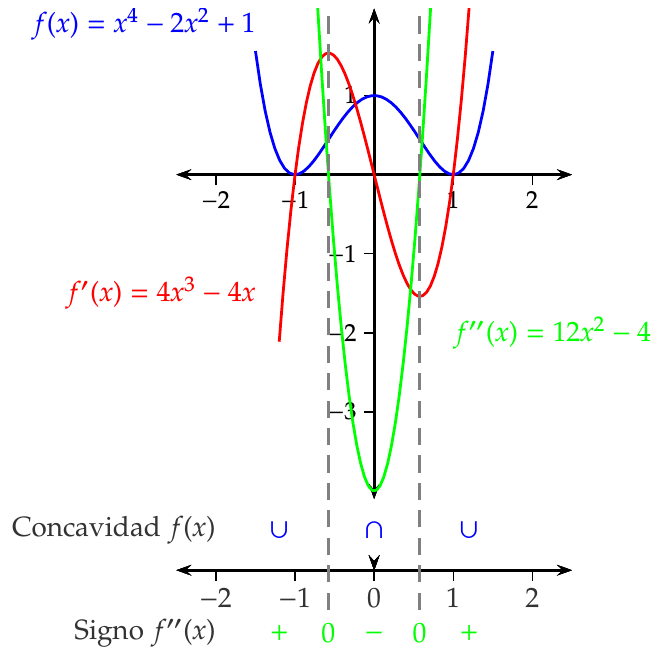
\includegraphics{img/derivadas/concavidad.png}

}

\caption{Estudio de la concavidad de una función.}

\end{figure}

\end{example}

\hypertarget{interpretaciuxf3n-cinemuxe1tica-de-la-derivada}{%
\section{Interpretación cinemática de la
derivada}\label{interpretaciuxf3n-cinemuxe1tica-de-la-derivada}}

\hypertarget{movimiento-rectiluxedneo}{%
\subsection{Movimiento rectilíneo}\label{movimiento-rectiluxedneo}}

Cuando una función \(f(t)\) describe la posición de un objeto móvil
sobre la recta real en el instante \(t\), tomando como referencia el
origen de coordenadas \(O\) y el vector unitario \(\mathbf{i}=(1)\), se
puede representar la posición \(P\) del móvil en cada instante \(t\)
mediante un vector \(\vec{OP}=x\mathbf{i}\) donde \(x=f(t)\).

\begin{figure}

{\centering 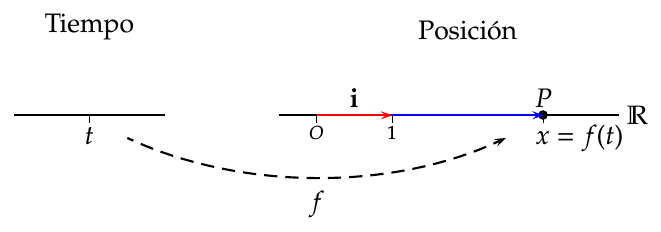
\includegraphics{img/derivadas/movimiento_rectilineo.png}

}

\caption{Interpretación cinemática del movimiento rectilíneo.}

\end{figure}

En este contexto, si se toman los instantes \(t=t_0\) y
\(t=t_0+\Delta t\), ambos del dominio \(I\) de \(f\), el vector

\[\mathbf{v}_m=\frac{f(t_0+\Delta t)-f(t_0)}{\Delta t}\]

que se conoce como \emph{velocidad media} del espacio recorrido por
\(f\) entre los instantes \(t_0\) y \(t_0+\Delta t\).

\begin{example}[]\protect\hypertarget{exm-movimiento-rectilineo}{}\label{exm-movimiento-rectilineo}

Un vehículo realiza un viaje de Madrid a Barcelona. Sea \(f(t)\) la
función que da la posición el vehículo en cada instante \(t\). Si el
vehículo parte de Madrid (km 0) a las 8 y llega a Barcelona (km 600) a
las 14 horas, entonces la velocidad media del vehículo en el trayecto es

\[
\mathbf{v}_m=\frac{f(14)-f(8)}{14-8}=\frac{600-0}{6} = 100 \mbox{ km/h}.
\]

Siguiendo en este mismo contexto del movimiento rectilíneo, la derivada
de \(f\) en el instante \(t=t_0\) es el vector

\[
\mathbf{v}=f'(t_0)=\lim_{\Delta x\rightarrow 0}\frac{f(t_0+\Delta t)-f(t_0)}{\Delta t},
\]

que se conoce, siempre que exista el límite, como \emph{velocidad
instantánea} o simplemente la \emph{velocidad} del espacio recorrido por
\(f\) en el instante \(t_0\).

Es decir, la derivada de la posición respecto del tiempo, es un campo de
vectores que recibe el nombre de \emph{velocidad a lo largo de la
trayectoria \(f\)}.

Siguiendo con el ejemplo anterior, lo que marca el velocímetro en un
determinado instante sería el módulo del vector velocidad en ese
instante.

\end{example}

\begin{tcolorbox}[enhanced jigsaw, colback=white, colbacktitle=quarto-callout-note-color!10!white, title=\textcolor{quarto-callout-note-color}{\faInfo}\hspace{0.5em}{Nota}, rightrule=.15mm, coltitle=black, arc=.35mm, opacityback=0, colframe=quarto-callout-note-color-frame, bottomtitle=1mm, titlerule=0mm, toptitle=1mm, bottomrule=.15mm, toprule=.15mm, breakable, opacitybacktitle=0.6, left=2mm, leftrule=.75mm]

También tiene sentido pensar en \(f(t)\) como una función que mide otras
magnitudes como por ejemplo la temperatura de un cuerpo, la
concentración de un gas, la cantidad de un compuesto en una reacción
química o el precio de las acciones de una compañía en cada instante
\(t\).

\end{tcolorbox}

\hypertarget{generalizaciuxf3n-al-movimiento-curviluxedneo}{%
\subsection{Generalización al movimiento
curvilíneo}\label{generalizaciuxf3n-al-movimiento-curviluxedneo}}

La derivada como velocidad a lo largo de una trayectoria en la recta
real puede generalizarse a trayectorias en cualquier espacio euclídeo
\(\mathbb{R}^n\).

Para el caso del plano real \(\mathbb{R}^2\), si \(f(t)\) describe la
posición de un objeto móvil en el plano en el instante \(t\), tomando
como referencia el origen de coordenadas \(O\) y los vectores
coordenados \(\{\mathbf{i}=(1,0),\mathbf{j}=(0,1)\}\), se puede
representar la posición \(P\) del móvil en cada instante \(t\) mediante
un vector \(\vec{OP}=x(t)\mathbf{i}+y(t)\mathbf{j}\) cuyas coordenadas

\[
\begin{cases}
x=x(t)\\
y=y(t)
\end{cases}
\quad
t\in I\subseteq \mathbb{R}
\]

se conocen como \emph{funciones coordenadas} de \(f\) y se escribe
\(f(t)=(x(t),y(t))\).

\begin{figure}

{\centering 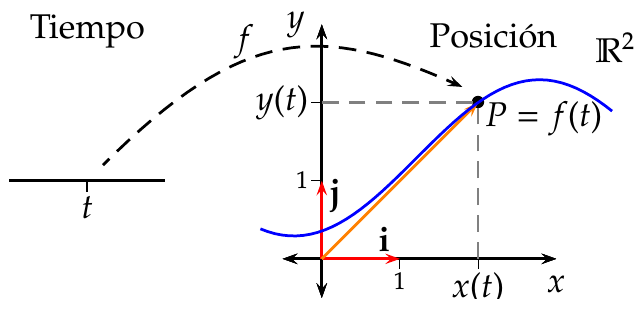
\includegraphics{img/derivadas/movimiento_curvilineo.png}

}

\caption{Interpretación cinemática del movimiento curvilineo.}

\end{figure}

\hypertarget{velocidad-en-una-trayectoria-curviluxednea-en-el-plano}{%
\subsubsection{Velocidad en una trayectoria curvilínea en el
plano}\label{velocidad-en-una-trayectoria-curviluxednea-en-el-plano}}

En este contexto de una trayectoria \(f(t)=(x(t),y(t))\) en el plano
real \(\mathbb{R}^2\), para un instante \(t=t_0\), si existe el vector

\[
\mathbf{v} = \lim_{\Delta t\rightarrow 0} \frac{f(t_0+\Delta t)-f(t_0)}{\Delta t},
\]

entonces \(f\) es derivable en el instante \(t=t_0\) y el vector
\(\mathbf{v}=f'(t_0)\) se conoce como \emph{velocidad} de \(f\) en ese
instante.

Como \(f(t)=(x(t),y(t))\),

\begin{align*}
f'(t)&=\lim_{\Delta t\rightarrow 0} \frac{f(t_0+\Delta t)-f(t_0)}{\Delta t}\\ 
&= \lim_{\Delta t\rightarrow 0} \frac{(x(t_0+\Delta t),y(t_0+\Delta t))-(x(t_0),y(t_0))}{\Delta t} \\
&=  \lim_{\Delta t\rightarrow 0} \left(\frac{x(t_0+\Delta t)-x(t_0)}{\Delta t},\frac{y(t_0+\Delta t)-y(t_0)}{\Delta t}\right) =\\
&= \left(\lim_{\Delta t\rightarrow 0}\frac{x(t_0+\Delta t)-x(t_0)}{\Delta t},\lim_{\Delta t\rightarrow 0}\frac{y(t_0+\Delta t)-y(t_0)}{\Delta t}\right) \\ 
&=
(x'(t_0),y'(t_0)).
\end{align*}

luego

\[
\mathbf{v} = x'(t_0)\mathbf{i}+y'(t_0)\mathbf{j}.
\]

\begin{example}[]\protect\hypertarget{exm-movimiento-curvilineo}{}\label{exm-movimiento-curvilineo}

Dada la trayectoria \(f(t) = (\cos(t),\operatorname{sen}(t))\),
\(t\in \mathbb{R}\), cuya imagen es la circunferencia de centro el
origen de coordenadas y radio 1, sus funciones coordenadas son
\(x(t) = \cos(t)\), \(y(t) = \operatorname{sen}(t)\),
\(t\in \mathbb{R}\), y su velocidad es

\[
\mathbf{v}=f'(t)=(x'(t),y'(t))=(-\operatorname{sen}(t), \cos(t).
\]

En el instante \(t=\pi/4\), el móvil estará en la posición
\(f(\pi/4) = (\cos(\pi/4),\operatorname{sen}(\pi/4)) =(\sqrt{2}/2,\sqrt{2}/2)\)
y se moverá con una velocidad
\(\mathbf{v}=f'(\pi/4)=(-\operatorname{sen}(\pi/4),\cos(\pi/4))=(-\sqrt{2}/2,\sqrt{2}/2)\).

\begin{figure}

{\centering 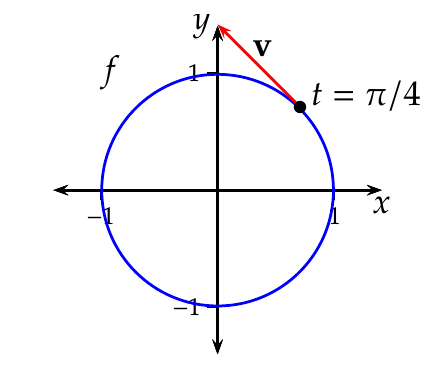
\includegraphics{img/derivadas/circunferencia.png}

}

\caption{Trayectoria de la circunferencia.}

\end{figure}

Obsérvese que el módulo del vector velocidad siempre será 1 ya que
\(\lvert \mathbf{v}\rvert = \sqrt{(-\operatorname{sen}(t))^2+(\cos(t))^2}=1\).

\end{example}

\hypertarget{recta-tangente-a-una-trayectoria}{%
\section{Recta tangente a una
trayectoria}\label{recta-tangente-a-una-trayectoria}}

\hypertarget{recta-tangente-a-una-trayectoria-en-el-plano}{%
\subsection{Recta tangente a una trayectoria en el
plano}\label{recta-tangente-a-una-trayectoria-en-el-plano}}

Los vectores paralelos a la velocidad \(\mathbf{v}\) se denominan
\emph{vectores tangentes} a la trayectoria \(f\) en el instante
\(t=t_0\), y la recta que pasa por \(P=f(t_0)\) dirigida por
\(\mathbf{v}\) es la recta tangente a \(f\) cuando \(t=t_0\).

\begin{definition}[Recta tangente a una
trayectoria]\protect\hypertarget{def-tangente-trayectoria}{}\label{def-tangente-trayectoria}

Dada una trayectoria \(f\) sobre el plano real \(\mathbb{R}^2\), se
llama \emph{recta tangente} a \(f\) en \(t=t_0\) a la recta de ecuación

\begin{align*}
l: (x,y)&= f(t_0)+tf'(t_0) = (x(t_0),y(t_0))+t(x'(t_0),y'(t_0))\\
&= (x(t_0)+tx'(t_0),y(t_0)+ty'(t_0)).
\end{align*}

\end{definition}

\begin{example}[]\protect\hypertarget{exm-tangente-trayectoria}{}\label{exm-tangente-trayectoria}

Se ha visto que para la trayectoria
\(f(t) = (\cos(t),\operatorname{sen}(t))\), \(t\in \mathbb{R}\), cuya
imagen es la circunferencia de centro el origen de coordenadas y radio
1, en el instante \(t=\pi/4\) la posición del móvil era
\(f(\pi/4)=(\sqrt{2}/2,\sqrt{2}/2)\) y su velocidad
\(\mathbf{v}=(-\sqrt{2}/2,\sqrt{2}/2)\), de modo que la recta tangente a
\(f\) en ese instante es

\begin{align*}
l &: X=f(\pi/2)+t\mathbf{v} = \left(\frac{\sqrt{2}}{2},\frac{\sqrt{2}}{2}\right)+t\left(\frac{-\sqrt{2}}{2},\frac{\sqrt{2}}{2}\right) \\ 
&=
\left(\frac{\sqrt{2}}{2}-t\frac{\sqrt{2}}{2},\frac{\sqrt{2}}{2}+t\frac{\sqrt{2}}{2}\right).
\end{align*}

\end{example}

De la ecuación vectorial de la recta tangente a \(f\) para \(t=t_0\), se
obtiene que sus funciones cartesianas son

\[
s\begin{cases}
x=x(t_0)+tx'(t_0)\\
y=y(t_0)+ty'(t_0)
\end{cases}
\quad t\in \mathbb{R},
\]

y despejando \(t\) en ambas ecuaciones e igualando se llega a la
ecuación cartesiana de la recta tangente

\[
\frac{x-x(t_0)}{x'(t_0)}=\frac{y-y(t_0)}{y'(t_0)},
\]

si \(x'(t_0)\neq 0\) e \(y'(t_0)\neq 0\), y de ahí a la ecuación en la
forma punto-pendiente

\[
y-y(t_0)=\frac{y'(t_0)}{x'(t_0)}(x-x(t_0)).
\]

Partiendo de la ecuación vectorial de la tangente del ejemplo anterior
\(l=\left(\frac{\sqrt{2}}{2}-t\frac{\sqrt{2}}{2},\frac{\sqrt{2}}{2}+t\frac{\sqrt{2}}{2}\right)\),
su ecuación cartesiana es

\[
\begin{gathered}
\frac{x-\sqrt{2}/2}{-\sqrt{2}/2} = \frac{y-\sqrt{2}/2}{\sqrt{2}/2}\Rightarrow\\
y-\sqrt{2}/2 = \frac{-\sqrt{2}/2}{\sqrt{2}/2}(x-\sqrt{2}/2) \Rightarrow \\
y=-x+\sqrt{2}.
\end{gathered}
\]

\hypertarget{recta-normal-a-una-trayectoria-en-el-plano}{%
\subsection{Recta normal a una trayectoria en el
plano}\label{recta-normal-a-una-trayectoria-en-el-plano}}

Se ha visto que la recta tangente a una trayectoria \(f\) cuando
\(t=t_0\) es la recta que pasa por el punto el punto \(P=f(t_0)\)
dirigida por el vector velocidad
\(\mathbf{v}=f'(t_0)=(x'(t_0),y'(t_0))\). Si en lugar de tomar ese
vector se toma como vector director el vector
\(\mathbf{w}=(y'(t_0),-x'(t_0))\), que es ortogonal a \(\mathbf{v}\), se
obtiene otra recta que se conoce como \emph{recta normal} a la
trayectoria \(f\) cuanto \(t=t_0\).

\begin{definition}[Recta normal a una
trayectoria]\protect\hypertarget{def-normal-trayectoria}{}\label{def-normal-trayectoria}

Dada una trayectoria \(f\) sobre el plano real \(\mathbb{R}^2\), se
llama \emph{recta normal} a \(f\) en \(t=t_0\) a la recta de ecuación

\begin{align*}
l: (x,y) &= (x(t_0),y(t_0))+t(y'(t_0),-x'(t_0)) =\\
&= (x(t_0)+ty'(t_0),y(t_0)-tx'(t_0)).
\end{align*}

\end{definition}

Su ecuación cartesiana es

\[
\frac{x-x(t_0)}{y'(t_0)} = \frac{y-y(t_0)}{-x'(t_0)},
\]

y su ecuación en la forma punto pendiente

\[
y-y(t_0) = \frac{-x'(t_0)}{y'(t_0)}(x-x(t_0)).
\]

\begin{tcolorbox}[enhanced jigsaw, colback=white, colbacktitle=quarto-callout-important-color!10!white, title=\textcolor{quarto-callout-important-color}{\faExclamation}\hspace{0.5em}{Importante}, rightrule=.15mm, coltitle=black, arc=.35mm, opacityback=0, colframe=quarto-callout-important-color-frame, bottomtitle=1mm, titlerule=0mm, toptitle=1mm, bottomrule=.15mm, toprule=.15mm, breakable, opacitybacktitle=0.6, left=2mm, leftrule=.75mm]

La recta normal es perpendicular a la recta tangente ya que sus vectores
directores son ortogonales.

\end{tcolorbox}

\begin{example}[]\protect\hypertarget{exm-normal-trayectoria}{}\label{exm-normal-trayectoria}

Siguiendo con el ejemplo de la trayectoria
\(f(t) = (\cos(t),\operatorname{sen}(t))\), \(t\in \mathbb{R}\), la
recta normal en el instante \(t=\pi/4\) es

\begin{align*}
l&: (x,y)=(\cos(\pi/2),\operatorname{sen}(\pi/2))+t(\cos(\pi/2),\operatorname{sen}(\pi/2)) =\\
& \left(\frac{\sqrt{2}}{2},\frac{\sqrt{2}}{2}\right)+t\left(\frac{\sqrt{2}}{2},\frac{\sqrt{2}}{2}\right)
=\left(\frac{\sqrt{2}}{2}+t\frac{\sqrt{2}}{2},\frac{\sqrt{2}}{2}+t\frac{\sqrt{2}}{2}\right),
\end{align*}

y su ecuación cartesiana es

\[
\frac{x-\sqrt{2}/2}{\sqrt{2}/2} = \frac{y-\sqrt{2}/2}{\sqrt{2}/2}\Rightarrow y-\sqrt{2}/2 = \frac{\sqrt{2}/2}{\sqrt{2}/2}(x-\sqrt{2}/2) \Rightarrow y=x.
\]

\begin{figure}

{\centering 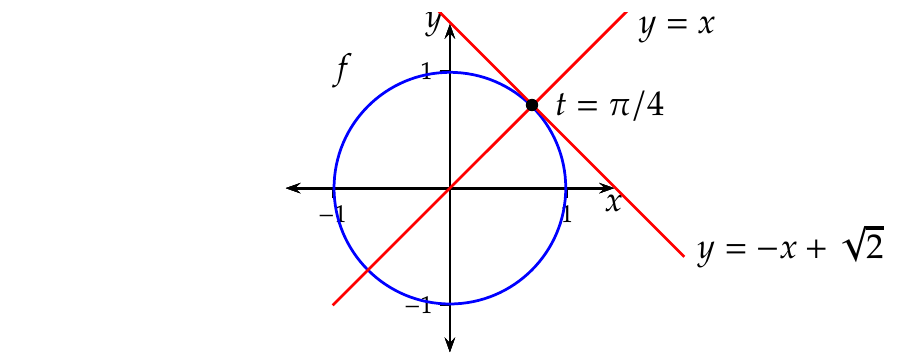
\includegraphics{img/derivadas/circunferencia_tangente_normal.png}

}

\caption{Tangente y normal a la trayectoria de una circunferencia.}

\end{figure}

\end{example}

\hypertarget{rectas-tangente-y-normal-a-una-funciuxf3n}{%
\subsection{Rectas tangente y normal a una
función}\label{rectas-tangente-y-normal-a-una-funciuxf3n}}

Un caso particular de las recta tangente y normal a una trayectoria son
la recta tangente y normal a una función de una variable real. Si se
tiene la función \(y=f(x)\), \(x\in I\subseteq \mathbb{R}\), una
trayectoria que traza la gráfica de \(f\) es
\(g(t) = (t,f(t)) \quad t\in I,\) y su velocidad es
\(g'(t) = (1,f'(t)),\) de modo que la recta tangente para \(t=a\) es

\[
\frac{x-a}{1} = \frac{y-f(a)}{f'(a)} \Rightarrow y-f(a) = f'(a)(x-a),
\]

y la recta normal es

\[
\frac{x-a}{f'(a)} = \frac{y-f(a)}{-1} \Rightarrow y-f(a) = \frac{-1}{f'(a)}(x-a),
\]

\begin{example}[]\protect\hypertarget{exm-tangente-normal-funcion-2}{}\label{exm-tangente-normal-funcion-2}

Dada la función \(y=f(x)=x^2\), la trayectoria que dibuja la gráfica de
esta función es \(g(t)=(t,t^2)\) y su velocidad es \(g'(t)=(1,2t)\), de
modo que en el punto \((1,1)\), que se alcanza en el instante \(t=1\),
la recta tangente es

\[
\frac{x-1}{1} = \frac{y-1}{2} \Rightarrow y-1 = 2(x-1) \Rightarrow y = 2x-1,
\]

y la recta normal es

\[
\frac{x-1}{2} = \frac{y-1}{-1} \Rightarrow y-1 = \frac{-1}{2}(x-1) \Rightarrow y = \frac{-x}{2}+\frac{3}{2}.
\]

\end{example}

\hypertarget{recta-tangente-a-una-trayectoria-en-el-espacio}{%
\subsection{Recta tangente a una trayectoria en el
espacio}\label{recta-tangente-a-una-trayectoria-en-el-espacio}}

El concepto de recta tangente a una trayectoria en el plano real puede
extenderse fácilmente a trayectorias en el espacio real
\(\mathbb{R}^3\).

Si \(f(t)=(x(t),y(t),z(t))\), \(t\in I\subseteq \mathbb{R}\), es una
trayectoria en el espacio real \(\mathbb{R}^3\), entonces el móvil que
recorre esta trayectoria en el instante \(t=t_0\), ocupará la posición
\(P=(x(t_0),y(t_0),z(t_0))\) y tendrá una velocidad
\(\mathbf{v}=f'(t)=(x'(t),y'(t),z'(t))\), de manera que la recta
tangente a \(f\) en ese instante será

\begin{align*}
l&: (x,y,z)=(x(t_0),y(t_0),z(t_0))+t(x'(t_0),y'(t_0),z'(t_0)) =\\
&= (x(t_0)+tx'(t_0),y(t_0)+ty'(t_0),z(t_0)+tz'(t_0)),
\end{align*}

cuyas ecuaciones cartesianas son

\[
\frac{x-x(t_0)}{x'(t_0)}=\frac{y-y(t_0)}{y'(t_0)}=\frac{z-z(t_0)}{z'(t_0)},
\]

siempre que \(x'(t_0)\neq 0\), \(y'(t_0)\neq 0\) y \(z'(t_0)\neq 0\).

\begin{example}[]\protect\hypertarget{exm-tangente-tracyectoria-espacio}{}\label{exm-tangente-tracyectoria-espacio}

Dada la trayectoria del espacio
\(f(t)=(\cos(t), \operatorname{sen}(t), t)\), \(t\in \mathbb{R}\), en el
instante \(t=\pi/2\), la trayectoria pasará por el punto

\[
f(\pi/2)=(\cos(\pi/2),\operatorname{sen}(\pi/2),\pi/2)=(0,1,\pi/2),
\]

con una velocidad

\[
\mathbf{v}=f'(\pi/2)=(-\operatorname{sen}(\pi/2),\cos(\pi/2), 1)=(-1,0,1),
\]

y la tangente en ese punto es

\[
l:(x,y,z)=(0,1,\pi/2)+t(-1,0,1) = (-t,1,t+\pi/2).
\]

\begin{figure}

{\centering 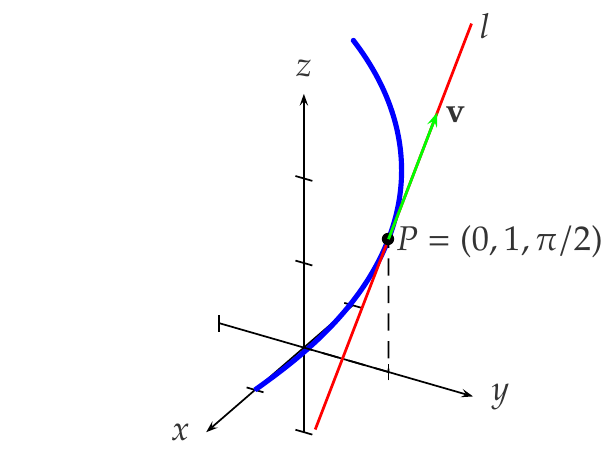
\includegraphics{img/derivadas/tangente_trayectoria_espacio.png}

}

\caption{Gráfica de la tangente a una trayectoria en el espacio.}

\end{figure}

\end{example}

\textbf{Ejemplo interactivo}

\hypertarget{sec-polinomios-taylor}{%
\section{Polinomios de Taylor}\label{sec-polinomios-taylor}}

\hypertarget{aproximaciuxf3n-de-una-funciuxf3n-mediante-un-polinomio}{%
\subsection{Aproximación de una función mediante un
polinomio}\label{aproximaciuxf3n-de-una-funciuxf3n-mediante-un-polinomio}}

Una aplicación muy útil de la derivada es la aproximación de funciones
mediante polinomios.

Los polinomios son funciones sencillas de calcular (mediante sumas y
productos), que tienen muy buenas propiedades:

\begin{itemize}
\tightlist
\item
  Están definidos en todos los números reales.
\item
  Son funciones continuas.
\item
  Son derivables hasta cualquier orden y sus derivadas son continuas.
\end{itemize}

En esta sección veremos cómo aproximar una función \(f(x)\) mediante un
polinomio \(p(x)\) cerca de un valor \(x=a\).

\hypertarget{aproximaciuxf3n-mediante-un-polinomio-de-grado-0}{%
\subsubsection{Aproximación mediante un polinomio de grado
0}\label{aproximaciuxf3n-mediante-un-polinomio-de-grado-0}}

Un polinomio de grado 0 tiene ecuación \[p(x) = c_0,\] donde \(c_0\) es
una constante.

Como el polinomio debe valer lo que la función en el punto \(a\), debe
cumplir

\[
p(a) = c_0 = f(a).
\]

En consecuencia, el polinomio de grado 0 que mejor aproxima a \(f\) en
un entorno de \(a\) es

\[
p(x) = f(a).
\]

\begin{figure}

{\centering 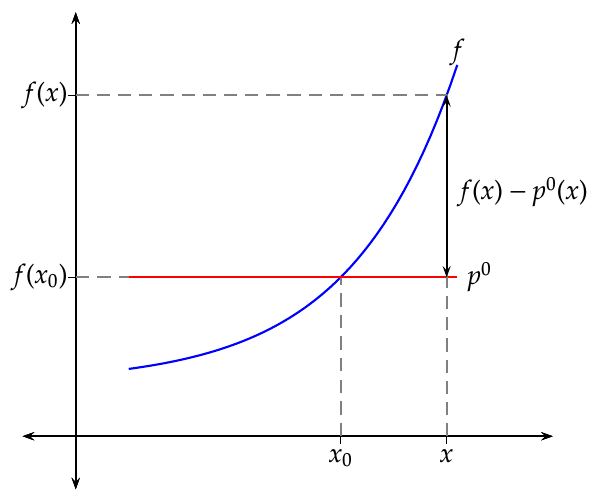
\includegraphics{img/derivadas/polinomio_grado_0.png}

}

\caption{Gráfica del polinomio de Taylor de grado 0}

\end{figure}

\hypertarget{aproximaciuxf3n-mediante-un-polinomio-de-grado-1}{%
\subsubsection{Aproximación mediante un polinomio de grado
1}\label{aproximaciuxf3n-mediante-un-polinomio-de-grado-1}}

Un polinomio de grado 1 es una recta y tiene ecuación

\[
p(x) = c_0+c_1x,
\]

aunque también puede escribirse

\[
p(x) = c_0+c_1(x-a).
\]

De entre todos los polinomios de grado 1, el que mejor aproxima a \(f\)
en entorno de \(a\) será el que cumpla las dos condiciones siguientes:

\begin{itemize}
\tightlist
\item
  \(p\) y \(f\) valen lo mismo en \(a\): \(p(a) = f(a)\),
\item
  \(p\) y \(f\) tienen la misma tasa de crecimiento en \(a\):
  \(p'(a) = f'(a)\).
\end{itemize}

Esta última condición nos asegura que en un entorno de \(a\), \(p\) y
\(f\) tienen aproximadamente la misma tendencia de crecimiento, pero
requiere que la función \(f\) sea derivable en \(a\).

Imponiendo las condiciones anteriores tenemos

\begin{itemize}
\tightlist
\item
  \(p(x)=c_0+c_1(x-a) \Rightarrow p(a)=c_0+c_1(a-a)=c_0=f(a)\),
\item
  \(p'(x)=c_1 \Rightarrow p'(a)=c_1=f'(a)\).
\end{itemize}

Así pues, el polinomio de grado 1 que mejor aproxima a \(f\) en un
entorno de \(a\) es

\[
p(x) = f(a)+f '(a)(x-a),
\]

que resulta ser la recta tangente a \(f\) en el punto \((a,f(a))\).

\begin{figure}

{\centering 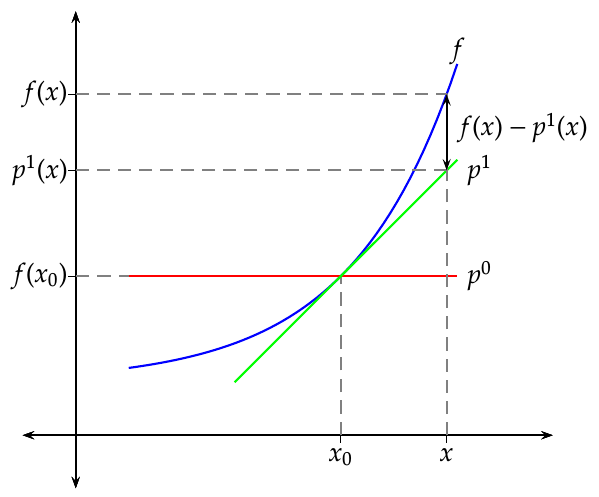
\includegraphics{img/derivadas/polinomio_grado_1.png}

}

\caption{Gráfica del polinomio de Taylor de grado 1}

\end{figure}

\hypertarget{aproximaciuxf3n-mediante-un-polinomio-de-grado-2}{%
\subsubsection{Aproximación mediante un polinomio de grado
2}\label{aproximaciuxf3n-mediante-un-polinomio-de-grado-2}}

Un polinomio de grado 2 es una parábola y tiene ecuación

\[
p(x) = c_0+c_1x+c_2x^2,
\]

aunque también puede escribirse

\[
p(x) = c_0+c_1(x-a)+c_2(x-a)^2.
\]

De entre todos los polinomio de grado 2, el que mejor aproxima a \(f\)
en entorno de \(a\) será el que cumpla las tres condiciones siguientes:

\begin{itemize}
\tightlist
\item
  \(p\) y \(f\) valen lo mismo en \(a\): \(p(a) = f(a)\),
\item
  \(p\) y \(f\) tienen la misma tasa de crecimiento en \(a\):
  \(p'(a) = f'(a)\).
\item
  \(p\) y \(f\) tienen la misma curvatura en \(a\): \(p''(a)=f''(a)\).
\end{itemize}

Esta última condición requiere que la función \(f\) sea dos veces
derivable en \(a\).

Imponiendo las condiciones anteriores tenemos

\begin{itemize}
\tightlist
\item
  \(p(x)=c_0+c_1(x-a)+c_2(x-a)^2 \Rightarrow p(a)=c_0=f(a)\),
\item
  \(p'(x)=c_1+2c_2(x-a) \Rightarrow p'(a)=c_1+2c_2(a-a)=c_1=f'(a)\),
\item
  \(p''(x)=2c_2 \Rightarrow p''(a)=2c_2=f''(a) \Rightarrow c_2=\frac{f''(a)}{2}\).
\end{itemize}

Así pues, el polinomio de grado 2 que mejor aproxima a \(f\) en un
entorno de \(a\) es

\[
p(x) = f(a)+f'(a)(x-a)+\frac{f''(a)}{2}(x-a)^2.
\]

\begin{figure}

{\centering 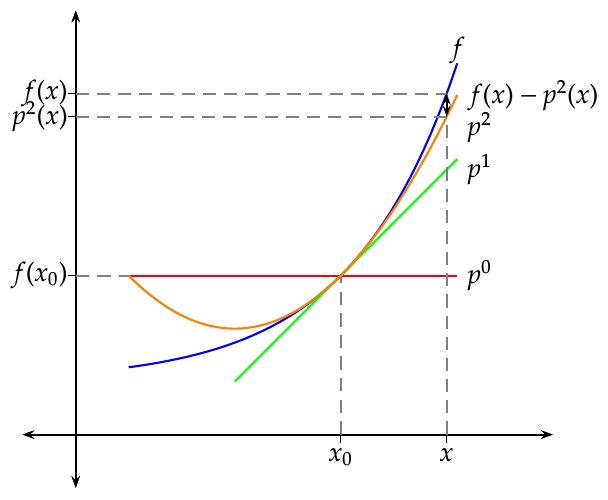
\includegraphics{img/derivadas/polinomio_grado_2.png}

}

\caption{Gráfica del polinomio de Taylor de grado 2}

\end{figure}

\hypertarget{aproximaciuxf3n-mediante-un-polinomio-de-grado-n}{%
\subsubsection{\texorpdfstring{Aproximación mediante un polinomio de
grado
\(n\)}{Aproximación mediante un polinomio de grado n}}\label{aproximaciuxf3n-mediante-un-polinomio-de-grado-n}}

Un polinomio de grado \(n\) tiene ecuación

\[
p(x) = c_0+c_1x+c_2x^2+\cdots +c_nx^n,
\]

aunque también puede escribirse

\[
p(x) = c_0+c_1(x-a)+c_2(x-a)^2+\cdots +c_n(x-a)^n.
\]

De entre todos los polinomio de grado \(n\), el que mejor aproxima a
\(f\) en entorno de \(a\) será el que cumpla las \(n+1\) condiciones
siguientes:

\begin{itemize}
\tightlist
\item
  \(p(a) = f(a)\),
\item
  \(p'(a) = f'(a)\),
\item
  \(p''(a)=f''(a)\),
\item
  \(\cdots\)
\item
  \(p^{(n}(a)=f^{(n}(a)\).
\end{itemize}

Las sucesivas derivadas de \(p\) valen

\begin{align*}
p(x) &= c_0+c_1(x-a)+c_2(x-a)^2+\cdots +c_n(x-a)^n,\\
p'(x) &= c_1+2c_2(x-a)+\cdots +nc_n(x-a)^{n-1},\\
p''(x) &= 2c_2+\cdots +n(n-1)c_n(x-a)^{n-2},\\
\vdots\\
p^{(n}(x) &= n(n-1)(n-2)\cdots 1c_n = n!c_n.
\end{align*}

Imponiendo las condiciones anteriores se tiene

\begin{itemize}
\tightlist
\item
  \(p(a) = c_0+c_1(a-a)+c_2(a-a)^2+\cdots +c_n(a-a)^n=c_0=f(a),\)
\item
  \(p'(a) = c_1+2c_2(a-a)+\cdots +nc_n(a-a)^{n-1}=c_1=f'(a),\)
\item
  \(p''(a) = 2c_2+\cdots +n(n-1)c_n(a-a)^{n-2}=2c_2=f''(a)\Rightarrow c_2=\frac{f''(a)}{2},\)
\item
  \(\cdots\)
\item
  \(p^{(n}(a)=n!c_n=f^{(n}(a)=c_n=\frac{f^{(n}(a)}{n!}\).
\end{itemize}

\begin{definition}[Polinomio de Taylor de orden \(n\) para \(f\) en el
punto
\(a\)]\protect\hypertarget{def-polinomio-taylor}{}\label{def-polinomio-taylor}

Dada una función \(f\), \(n\) veces derivable en \(x=a\), se define el
\emph{polinomio de Taylor} de orden \(n\) para \(f\) en \(a\) como

\begin{align*}
p_{f,a}^n(x)&=f(a)+f'(a)(x-a)+\frac{f''(a)}{2}(x-a)^2+\cdots +\frac{f^{(n}(a)}{n!}(x-a)^n = \\ &=\sum_{i=0}^{n}\frac{f^{(i}(a)}{i!}(x-a)^i,
\end{align*}

o bien, escribiendo \(x=a+h\)

\begin{align*}
p_f^n(a+h) &= f(a)+f'(a)h+\frac{f''(a)}{2}h^2+\cdots +\frac{f^{(n}(a)}{n!}h^n =\\
&= \sum_{i=0}^{n}\frac{f^{(i}(a)}{i!}h^i.
\end{align*}

\end{definition}

\begin{tcolorbox}[enhanced jigsaw, colback=white, colbacktitle=quarto-callout-important-color!10!white, title=\textcolor{quarto-callout-important-color}{\faExclamation}\hspace{0.5em}{Importante}, rightrule=.15mm, coltitle=black, arc=.35mm, opacityback=0, colframe=quarto-callout-important-color-frame, bottomtitle=1mm, titlerule=0mm, toptitle=1mm, bottomrule=.15mm, toprule=.15mm, breakable, opacitybacktitle=0.6, left=2mm, leftrule=.75mm]

El polinomio de Taylor de orden \(n\) para \(f\) en \(a\) es el
polinomio de orden \(n\) que mejor aproxima a \(f\) alrededor de \(a\),
ya que es el único que cumple las \(n+1\) condiciones anteriores.

\end{tcolorbox}

\begin{example}[]\protect\hypertarget{exm-polinomio-taylor}{}\label{exm-polinomio-taylor}

Vamos a aproximar la función \(f(x)=\log x\) en un entorno del punto
\(1\) mediante un polinomio de grado \(3\).

La ecuación del polinomio de Taylor de orden \(3\) para \(f\) en el
punto \(1\) es

\[
p_{f,1}^3(x)=f(1)+f'(1)(x-1)+\frac{f''(1)}{2}(x-1)^2+\frac{f'''(1)}{3!}(x-1)^3.
\]

Calculamos las tres primeras derivadas de \(f\) en \(1\):

\[
\begin{array}{lll}
f(x)=\log x & \quad & f(1)=\log 1 =0,\\
f'(x)=1/x & & f'(1)=1/1=1,\\
f''(x)=-1/x^2 & & f''(1)=-1/1^2=-1,\\
f'''(x)=2/x^3 & & f'''(1)=2/1^3=2.
\end{array}
\]

Sustituyendo en la ecuación del polinomio se tiene

\[
p_{f,1}^3(x)=0+1(x-1)+\frac{-1}{2}(x-1)^2+\frac{2}{3!}(x-1)^3= \frac{2}{3}x^3-\frac{3}{2}x^2+3x-\frac{11}{6}.
\]

\begin{figure}

{\centering 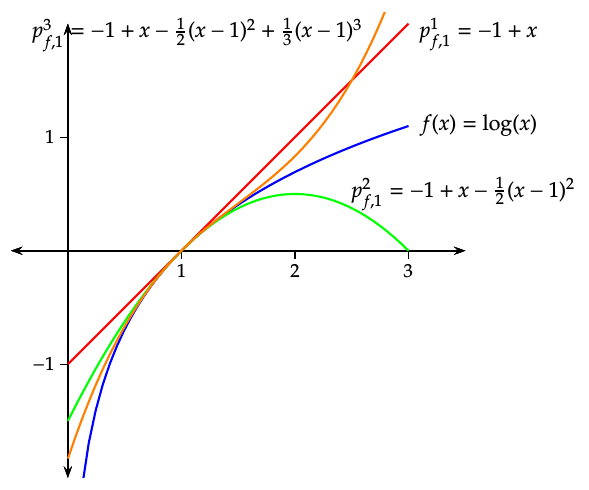
\includegraphics{img/derivadas/polinomio_taylor_logaritmo.png}

}

\caption{Gráfica del polinomio de Taylor del logaritmo}

\end{figure}

\end{example}

\hypertarget{polinomio-de-maclaurin-de-orden-n}{%
\subsection{\texorpdfstring{Polinomio de Maclaurin de orden
\(n\)}{Polinomio de Maclaurin de orden n}}\label{polinomio-de-maclaurin-de-orden-n}}

La ecuación del polinomio de Taylor se simplifica cuando el punto en
torno al cual queremos aproximar es el \(0\).

\begin{definition}[Polinomio de Maclaurin de orden \(n\) para
\(f\)]\protect\hypertarget{def-polinomio-maclaurin}{}\label{def-polinomio-maclaurin}

Dada una función \(f\), \(n\) veces derivable en \(0\), se define el
\emph{polinomio de Maclaurin} de orden \(n\) para \(f\) como

\begin{align*}
p_{f,0}^n(x) &= f(0)+f'(0)x+\frac{f''(0)}{2}x^2+\cdots +\frac{f^{(n}(0)}{n!}x^n =\\
&= \sum_{i=0}^{n}\frac{f^{(i}(0)}{i!}x^i.
\end{align*}

\end{definition}

\begin{example}[]\protect\hypertarget{exm-polinomio-maclaurin}{}\label{exm-polinomio-maclaurin}

Vamos a aproximar la función \(f(x)=\operatorname{sen} x\) en un entorno
del punto \(0\) mediante un polinomio de grado \(3\).

La ecuación del polinomio de Maclaurin de orden \(3\) para \(f\) es

\[
p_{f,0}^3(x)=f(0)+f'(0)x+\frac{f''(0)}{2}x^2+\frac{f'''(0)}{3!}x^3.
\]

Calculamos las tres primeras derivadas de \(f\) en \(0\):

\[
\begin{array}{lll}
f(x)=\operatorname{sen} x & \quad & f(0)=\operatorname{sen} 0 =0,\\
f'(x)=\cos x & & f'(0)=\cos 0=1,\\
f''(x)=-\operatorname{sen} x & & f''(0)=-\operatorname{sen} 0=0,\\
f'''(x)=-\cos x & & f'''(0)=-\cos 0=-1.
\end{array}
\]

Sustituyendo en la ecuación del polinomio obtenemos

\[
p_{f,0}^3(x)=0+1\cdot x+\frac{0}{2}x^2+\frac{-1}{3!}x^3= x-\frac{x^3}{6}.
\]

\begin{figure}

{\centering 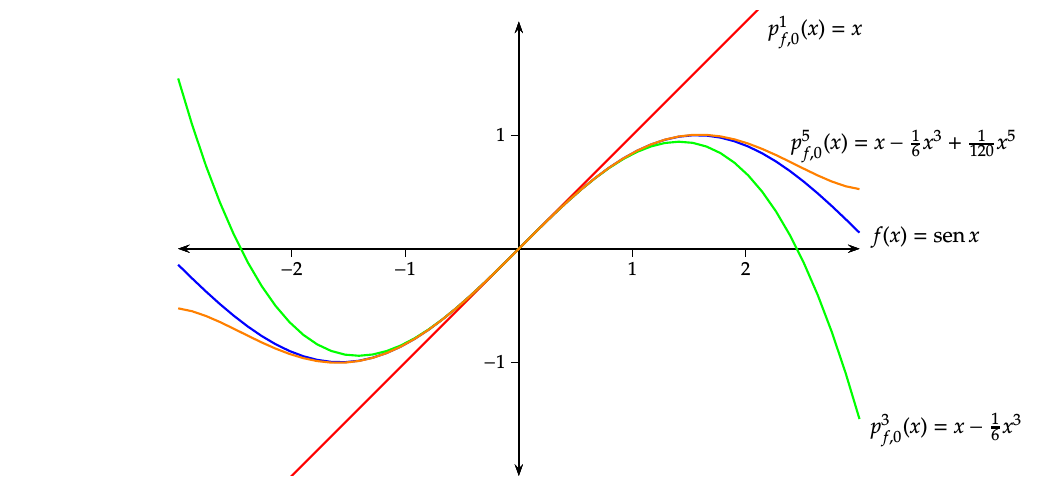
\includegraphics{img/derivadas/polinomio_mclaurin_seno.png}

}

\caption{Gráfica del polinomio de Maclaurin del seno}

\end{figure}

\end{example}

\hypertarget{polinomios-de-maclaurin-de-funciones-elementales}{%
\subsection{Polinomios de Maclaurin de funciones
elementales}\label{polinomios-de-maclaurin-de-funciones-elementales}}

La siguiente tabla recoge los polinomios de Taylor de orden \(n\) de
algunas funciones elementales habituales.

\begin{longtable}[]{@{}
  >{\centering\arraybackslash}p{(\columnwidth - 2\tabcolsep) * \real{0.5000}}
  >{\centering\arraybackslash}p{(\columnwidth - 2\tabcolsep) * \real{0.5000}}@{}}
\toprule\noalign{}
\begin{minipage}[b]{\linewidth}\centering
\(f(x)\)
\end{minipage} & \begin{minipage}[b]{\linewidth}\centering
\(p_{f,0}^n(x)\)
\end{minipage} \\
\midrule\noalign{}
\endhead
\bottomrule\noalign{}
\endlastfoot
\(e^x\) &
\(\displaystyle 1 + x + \frac{x^2}{2!} + \frac{x^3}{3!} + \cdots + \frac{x^n}{n!} = \sum_{i=0}^n \frac{x^i}{i!}\) \\
\(\log(1+x)\) &
\(\displaystyle x-\frac{x^2}{2}+\frac{x^3}{3}-\cdots +(-1)^{n-1}\frac{x^n}{n} = \sum_{i=0}^n (-1)^{i-1}\frac{x^i}{i}\) \\
\(\operatorname{sen}(x)\) &
\(\displaystyle x-\frac{x^3}{3!}+\frac{x^5}{5!}-\cdots +(-1)^k\frac{x^{2k-1}}{(2k-1)!} = \sum_{i=0}^k (-1)^i\frac{x^{2i-1}}{(2i-1)!}\)
si \(n=2k\) o \(n=2k-1\) \\
\(\cos(x)\) &
\(\displaystyle 1-\frac{x^2}{2!}+\frac{x^4}{4!}-\cdots +(-1)^k\frac{x^{2k}}{(2k)!} = \sum_{i=0}^k (-1)^i\frac{x^{2i}}{(2i)!}\)
si \(n=2k\) o \(n=2k+1\) \\
\(\operatorname{arctg}(x)\) &
\(\displaystyle x-\frac{x^3}{3}+\frac{x^5}{5}-\cdots +(-1)^k\frac{x^{2k-1}}{(2k-1)} = \sum_{i=0}^k (-1)^i\frac{x^{2i-1}}{(2i-1)}\)
si \(n=2k\) o \(n=2k-1\) \\
\end{longtable}

\hypertarget{resto-de-taylor}{%
\subsection{Resto de Taylor}\label{resto-de-taylor}}

Los polinomios de Taylor permiten calcular el valor aproximado de una
función cerca de un valor \(a\), pero siempre se comete un error en
dicha aproximación.

\begin{definition}[Resto de
Taylor]\protect\hypertarget{def-resto-taylor}{}\label{def-resto-taylor}

Si \(f\) es una función para la que existe el su polinomio de Taylor de
orden \(n\) en \(a\), \(p_{f,a}^n\), entonces se define el \emph{resto
de Taylor} de orden \(n\) para \(f\) en \(a\) como

\[
r_{f,a}^n(x)=f(x)-p_{f,a}^n(x).
\]

\end{definition}

El resto mide el error cometido al aproximar \(f(x)\) mediante
\(p_{f,a}^n(x)\) y permite expresar la función \(f\) como la suma de un
polinomio de Taylor más su resto correspondiente:

\[
f(x)=p_{f,a}^n(x) + r_{f,a}^n(x).
\]

Esta expresión se conoce como \emph{fórmula de Taylor} de orden \(n\)
para \(f\) en \(a\). Se pude demostrar, además, que

\[
\lim_{h\rightarrow 0}\frac{r_{f,a}^n(a+h)}{h^n}=0,
\]

lo cual indica que el resto \(r_{f,a}^n(a+h)\) es mucho menor que
\(h^n\).

\begin{theorem}[Forma de Lagrange del resto de
Taylor]\protect\hypertarget{thm-forma-Lagrange-resto}{}\label{thm-forma-Lagrange-resto}

Si \(f\) es una función tal que \(f^{(n+1}(t)\) es continua en un
intervalo que incluye a \(a\) y \(x\), entonces

\[
R^n_{f,a}(x)=\frac{f^{(n+1}(c)}{(n+1)!}(x-a)^{n+1}
\]

para algún \(c\) entre \(a\) y \(x\).

\end{theorem}

La forma de Lagrange del resto de Taylor permite, en muchas ocasiones,
dar una cota de las aproximaciones realizadas mediante un polinomio de
Taylor.

\begin{example}[]\protect\hypertarget{exm-cota-resto}{}\label{exm-cota-resto}

Dada la función \(f(x)=\cos(x)\) el polinomio de MacLaurin de cuarto
grado de \(f\) es

\[
P^4_{f,0}(x)=1-\frac{x^2}{2}+\frac{x^4}{4!}.
\]

Sustituyendo en \(x=0.1\) se tiene que
\(\cos(0.1)\approx P^2_{f,0}(0.1) = 1-\frac{0.1^2}{2}+\frac{0.1^4}{4!}= 0.9950041667\).

Para obtener una cota del error cometido, aplicando el teorema anterior
se tiene que

\[
R^4_{f,0}(0.1)=\frac{f^{5}(c)}{5!}0.1^5 = \frac{-\operatorname{sen}(c)}{5!}0.1^5 \mbox{ con }c\in [0,0.1].
\]

Como \(|\operatorname{sen}(x)|\leq 1\) \(\forall x\in\mathbb{R}\), se
tiene que

\[
|R^4_{f,0}(0.1)|\leq \frac{0.1^5}{5!} = 8.3\cdot 10^{-8},
\]

que es una cota del error cometido en la aproximación.

\end{example}

\bookmarksetup{startatroot}

\hypertarget{series-de-nuxfameros-reales}{%
\chapter{Series de números reales}\label{series-de-nuxfameros-reales}}

En este capítulo se estudian las \emph{series} de números reales, un
tipo especial de sucesiones que se construyen a partir de la suma de los
términos de otras sucesiones. Este tipo de sucesiones son las más
importantes del Análisis pues, como se verá más adelante, aparecen en
multitud de contextos reales.

Como ejemplo introductorio puede servir la
\href{https://es.wikipedia.org/wiki/Paradojas_de_Zen\%C3\%B3n\#Paradoja_de_la_dicotom\%C3\%ADa}{paradoja
de la dicotomía de Zenon}, que establece que para que un corredor pueda
recorrer una distancia hasta la meta, primero tiene que recorrer la
mitad de la distancia, después la mitad de la distancia restante,
después la mitad de la distancia restante, y así hasta el infinito, por
lo que, aparentemente, nunca llegaría a la meta.

\begin{figure}

{\centering 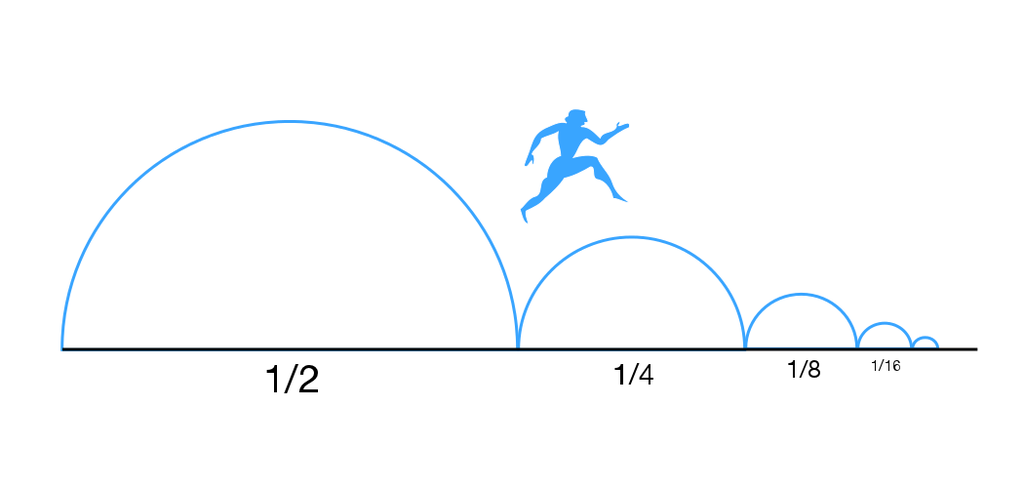
\includegraphics{img/series/paradoja-dicotomia-zenon.png}

}

\caption{Paradoja de la dicotomía de Zenon.(imagen tomada de Wikipedia)}

\end{figure}

La distancia recorrida por el corredor puede expresarse como una suma
infinita

\[
\frac{1}{2}+\frac{1}{4}+\frac{1}{8}+\frac{1}{16}+\frac{1}{32}+\cdots
\]

que puede representarse, de manera más concisa, mediante el sumatorio

\[
\sum_{n=1}^\infty \frac{1}{2^n}.
\]

Por supuesto, por experiencia, sabemos que el corredor acaba llegando a
la meta, por lo que la suma de estas distancias debe ser la distancia
total, es decir,

\[
\sum_{n=1}^\infty \frac{1}{2^n} = 1.
\]

En este capítulo estudiaremos estas sumas infinitas y veremos técnicas
para calcularlas cuando existan.

\hypertarget{concepto-de-serie}{%
\section{Concepto de serie}\label{concepto-de-serie}}

\begin{definition}[Serie]\protect\hypertarget{def-serie}{}\label{def-serie}

Dada una sucesión de números reales \((a_n)_{n=1}^\infty\), se llama
\emph{serie} de término general \(a_n\) a la sucesión
\((A_n)_{n=1}^\infty\), cuyos términos se obtienen sumando
consecutivamente los \(n\) primeros términos de \((a_n)_{n=1}^\infty\),
es decir,

\[
(A_n)_{n=1}^\infty= \left(\sum_{i=1}^na_i\right)_{n=1}^\infty.
\]

El número \(A_n=\sum_{i=1}^n a_i\) se llama \emph{suma parcial de orden}
\(n\) de la serie, y habitualmente utilizaremos la notación \(\sum a_n\)
para referirnos a la serie de término general \(n\).

\end{definition}

\begin{tcolorbox}[enhanced jigsaw, colback=white, colbacktitle=quarto-callout-important-color!10!white, title=\textcolor{quarto-callout-important-color}{\faExclamation}\hspace{0.5em}{Importante}, rightrule=.15mm, coltitle=black, arc=.35mm, opacityback=0, colframe=quarto-callout-important-color-frame, bottomtitle=1mm, titlerule=0mm, toptitle=1mm, bottomrule=.15mm, toprule=.15mm, breakable, opacitybacktitle=0.6, left=2mm, leftrule=.75mm]

Debe quedar claro que una serie no es una suma, sino una sucesión cuyos
términos se forman mediante sumas de los términos de otra sucesión. Por
tanto, todos lo visto en el
\href{https://aprendeconalf.es/analisis-manual/sucesiones.html}{capítulo
de sucesiones} es válido también para series.

\end{tcolorbox}

\begin{example}[]\protect\hypertarget{exm-serie}{}\label{exm-serie}

A partir de la sucesión \(\left(\frac{1}{n}\right)_{n=1}^\infty\), se
puede construir la serie \(\sum \frac{1}{n}=(A_n)_{n=1}^\infty\) tal que

\begin{align*}
A_1 &= 1\\ 
A_2 &= 1+\frac{1}{2}\\ 
A_3 &= 1+\frac{1}{2}+\frac{1}{3}\\ 
\vdots\\ 
A_n &= 1+\frac{1}{2}+\frac{1}{3}+\cdots \frac{1}{n} = \sum_{i=1}^n\frac{1}{i} 
\end{align*}

Esta serie se conoce como \emph{serie armónica}. En la siguiente gráfica
se puede apreciar cómo evoluciona la sucesión de sus sumas parciales.

\end{example}

En ocasiones es posible expresar el valor de la suma parcial de orden
\(n\) mediante una fórmula explícita que depende de \(n\) y que se
conoce como \emph{forma cerrada} de la serie. Si una serie puede
expresarse mediante una forma cerrada, resulta más rápido calcular el
valor de la suma parcial de orden \(n\) mediante la forma cerrada, que
haciendo la propia suma de los \(n\) primeros términos de la sucesión.

\begin{example}[]\protect\hypertarget{exm-serie-forma-cerrada}{}\label{exm-serie-forma-cerrada}

Dada la serie \(\sum n\), su suma parcial de orden \(n\)
\(A_n=\sum_{i=1}^n n\) puede expresarse mediante la forma cerrada
\(A_n = \frac{1}{2}n(n+1)\).

\end{example}

\hypertarget{convergencia-de-series}{%
\section{Convergencia de series}\label{convergencia-de-series}}

\begin{definition}[Serie
convergente]\protect\hypertarget{def-serie-convergente}{}\label{def-serie-convergente}

Se dice que una serie \(\sum a_n\) es \emph{convergente}, o que la
sucesión \((a_n)_{n=1}^\infty\) es sumable, si la sucesión de las sumas
parciales \(\left(\sum_{i=1}^n a_i\right)_{n=1}^\infty\) es convergente,
y en tal caso, utilizaremos la notación \(\sum_{n=1}^\infty a_n\) para
referirnos a su límite.

\[
\sum_{n=1}^{\infty} a_n=\lim A_n = \lim_{n\to\infty} \sum_{i=1}^n a_i.
\]

\end{definition}

Si una serie no es convergente, se dice que es \emph{divergente}.

A veces interesa considerar series que empiezan en un índice distinto de
1. En tal caso, se usará la notación \(\sum_{n\geq k}a_n\) para
referirse a la serie, y \(\sum_{n=k}^\infty a_n\) para referirse a su
límite.

\begin{example}[]\protect\hypertarget{exm-serie-paradoja-zenon}{}\label{exm-serie-paradoja-zenon}

Veamos que la serie \(\sum \left(\frac{1}{2}\right)^n\) de la paradoja
de la dicotomía de Zenon converge.

\[
\sum_{i=1}^n \left(\frac{1}{2}\right)^i = 1 + \frac{1}{2} + \cdots +\frac{1}{2^n} = \frac{1-\frac{1}{2^{n+1}}}{1-\frac{1}{2}} = 2-\frac{1}{2^n}.
\]

Y, por tanto,

\[
\sum_{n=1}^\infty \left(\frac{1}{2}\right)^n = \lim_{n\to\infty} \sum_{i=1}^n \left(\frac{1}{2}\right)^i = \lim_{n\to\infty} 2-\frac{1}{2^n} = 2.
\]

\end{example}

\begin{example}[]\protect\hypertarget{exm-serie-divergente}{}\label{exm-serie-divergente}

La serie \(\sum (-1)^n\) diverge. Para probarlo, basta con ver que las
sumas parciales de orden \(n\) forman una sucesión alternada.

\begin{align*}
A_1 &= -1\\ 
A_2 &= -1+ (-1)^2 = 0 \\ 
A_3 &= -1+ (-1)^2 + (-1)^3 = -1\\ 
A_4 &= -1+ (-1)^2 + (-1)^3 + (-1)^4= 0\\ 
\vdots 
\end{align*}

y por tanto, \((A_n)_{n=1}^\infty\) diverge.

\end{example}

\begin{example}[]\protect\hypertarget{exm-divergencia-serie-armonica}{}\label{exm-divergencia-serie-armonica}

La serie armónica \(\sum \frac{1}{n}\) diverge. Una prueba bastante
intuitiva se debe a
\href{https://es.wikipedia.org/wiki/Nicol\%C3\%A1s_Oresme}{Nicole
Oresme} y se basa en agrupar los términos de la serie en potencias de 2
de la siguiente manera

\[
\sum_{n=1}^\infty \frac{1}{n} = 1 + \frac{1}{2} + \left[\frac{1}{3}+\frac{1}{4}\right] + \left[\frac{1}{5}+\frac{1}{6}+\frac{1}{7}+\frac{1}{8}\right] + \cdots
\]

Es fácil ver que los términos de esta serie son mayores que los de esta
otra

\[
\begin{gathered}
1 + \frac{1}{2} + \left[\frac{1}{4}+\frac{1}{4}\right] + \left[\frac{1}{8}+\frac{1}{8}+\frac{1}{8}+\frac{1}{8}\right] + \cdots \\ 
= 1 +\frac{1}{2} + \frac{1}{2} + \frac{1}{2} + \cdots
\end{gathered}
\] que claramente diverge, por lo que la serie armónica también diverge.

Sin embargo, la serie armónica alternada \(\sum \frac{(-1)^{n+1}}{n}\)
converge. La prueba es una consecuencia de la serie de Taylor para el
logaritmo y se deja como ejercicio.

\end{example}

\begin{proposition}[]\protect\hypertarget{prp-series-iguales-excepto-n-terminos}{}\label{prp-series-iguales-excepto-n-terminos}

Dadas dos sucesiones \((a_n)_{n=1}^\infty\) y \((b_n)_{n=1}^\infty\)
tales que \(a_n=b_n\) \(\forall n>k\in\mathbb{N}\). Entonces,
\(\sum a_n\) converge si y solo si \(\sum b_n\) converge, y en caso de
converger se cumple que \[
\sum_{n=1}^\infty a_n-\sum_{i=1}^{k}a_i=\sum_{n=1}^\infty b_n-\sum_{i=1}^{k}b_i.
\]

\end{proposition}

\begin{tcolorbox}[enhanced jigsaw, colback=white, colbacktitle=quarto-callout-note-color!10!white, title=\textcolor{quarto-callout-note-color}{\faInfo}\hspace{0.5em}{Demostración}, rightrule=.15mm, coltitle=black, arc=.35mm, opacityback=0, colframe=quarto-callout-note-color-frame, bottomtitle=1mm, titlerule=0mm, toptitle=1mm, bottomrule=.15mm, toprule=.15mm, breakable, opacitybacktitle=0.6, left=2mm, leftrule=.75mm]

\begin{proof}

Pongamos \(A_n=a_1+a_2+\cdots+a_n\), \(B_n=b_1+b_2+\cdots+b_n\),
\(\alpha=\sum_{i=1}^{k}a_i\), \(\beta=\sum_{i=1}^{k}b_i\). Las
afirmaciones hechas se deducen todas de que para todo \(n\ge q+1\) se
verifica la igualdad:

Como \(a_n=b_n\) \(\forall n>k\in\mathbb{N}\), se tiene que

\[
\sum_{i=k+1}^\infty a_i=\sum_{i=k+1}^\infty b_i
\]

y, por tanto,

\[
\sum_{n=1}^\infty a_n-\sum_{i=1}^k a_i= \sum_{i=k+1}^\infty a_i=\sum_{i=k+1}^\infty b_i =  \sum_{n=1}^\infty b_n-\sum_{i=1}^{k}b_i.
\]

\end{proof}

\end{tcolorbox}

\begin{proposition}[]\protect\hypertarget{prp-linealidad-series-convergentes}{}\label{prp-linealidad-series-convergentes}

Dadas dos series convergentes \(\sum a_n\) y \(\sum b_n\), entonces se
cumple

\begin{enumerate}
\def\labelenumi{\alph{enumi}.}
\tightlist
\item
  La serie \(\sum (a_n+b_n)\) es convergente y
  \(\sum_{n=1}^\infty (a_n+b_n) = \sum_{n=1}^\infty a_n +\sum_{n=1}^\infty b_n\).
\item
  La serie \(\sum (c\cdot a_n)\) es convergente y
  \(\sum_{n=1}^\infty (c\cdot a_n) = c\sum_{n=1}^\infty a_n\).
\end{enumerate}

\end{proposition}

\begin{tcolorbox}[enhanced jigsaw, colback=white, colbacktitle=quarto-callout-note-color!10!white, title=\textcolor{quarto-callout-note-color}{\faInfo}\hspace{0.5em}{Demostración}, rightrule=.15mm, coltitle=black, arc=.35mm, opacityback=0, colframe=quarto-callout-note-color-frame, bottomtitle=1mm, titlerule=0mm, toptitle=1mm, bottomrule=.15mm, toprule=.15mm, breakable, opacitybacktitle=0.6, left=2mm, leftrule=.75mm]

\begin{proof}

Sean \((A_n)_{n=1}^\infty\) y \((B_n)_{n=1}^\infty\) las sucesiones de
las sumas parciales de \(\sum a_n\) y \(\sum b_n\) respectivamente. Si
\(\sum a_n\) y \(\sum b_n\) convergen, entonces \((A_n)_{n=1}^\infty\) y
\((B_n)_{n=1}^\infty\) convergen y, por las propiedades de las
sucesiones convergentes, \((A_n+B_n)_{n=1}^\infty\) converge, y además

\[
\lim_{n\to\infty} A_n+B_n = \lim_{n\to\infty}A_n+\lim_{n\to\infty}B_n.
\]

En consecuencia, \(\sum (a_n+b_n)\) converge y
\(\sum_{n=1}^\infty (a_n+b_n) = \sum_{n=1}^\infty a_n+\sum_{n=1}^\infty b_n\).

\end{proof}

\end{tcolorbox}

\begin{theorem}[Criterio de
Cauchy]\protect\hypertarget{thm-criterio-cauchy-series}{}\label{thm-criterio-cauchy-series}

La serie \(\sum a_n\) converge si y solo si para cada \(\varepsilon>0\)
existe \(k\in\mathbb{N}\) tal que

\[
|a_{n+1}+a_{n+2}+\cdots+a_m|<\varepsilon\ \forall m>n\geq k.
\]

\end{theorem}

\begin{tcolorbox}[enhanced jigsaw, colback=white, colbacktitle=quarto-callout-note-color!10!white, title=\textcolor{quarto-callout-note-color}{\faInfo}\hspace{0.5em}{Demostración}, rightrule=.15mm, coltitle=black, arc=.35mm, opacityback=0, colframe=quarto-callout-note-color-frame, bottomtitle=1mm, titlerule=0mm, toptitle=1mm, bottomrule=.15mm, toprule=.15mm, breakable, opacitybacktitle=0.6, left=2mm, leftrule=.75mm]

\begin{proof}

Sea \((A_n)_{n=1}^\infty\) la sucesión de las sumas parciales de
\(\sum a_n\). Entonces, \(\sum a_n\) converge si y solo si
\((A_n)_{n=1}^\infty\) converge, y por el criterio de convergencia de
Cauchy para sucesiones (Teorema~\ref{thm-criterio-convergencia-cauchy})
esto es equivalente a que \((A_n)_{n=1}^\infty\) es una sucesión de
Cauchy, de manera que se cumple que para cualquier \(\varepsilon>0\)
existe un \(k\in\mathbb{N}\) tal que \(|A_m-A_n|<\varepsilon\)
\(\forall m>n\geq k\), lo que es equivalente a que
\(|a_{n+1}+a_{n+2}+\cdots+a_m|<\varepsilon\ \forall m>n\geq k\).

\end{proof}

\end{tcolorbox}

El siguiente teorema establece una condición necesaria para la
convergencia de una serie.

\begin{theorem}[Criterio de
divergencia]\protect\hypertarget{thm-criterio-divergencia-series}{}\label{thm-criterio-divergencia-series}

Dada una serie \(\sum a_n\), si \(\lim_{n\to\infty} a_n \neq 0\),
entonces la serie diverge.

\end{theorem}

\begin{tcolorbox}[enhanced jigsaw, colback=white, colbacktitle=quarto-callout-note-color!10!white, title=\textcolor{quarto-callout-note-color}{\faInfo}\hspace{0.5em}{Demostración}, rightrule=.15mm, coltitle=black, arc=.35mm, opacityback=0, colframe=quarto-callout-note-color-frame, bottomtitle=1mm, titlerule=0mm, toptitle=1mm, bottomrule=.15mm, toprule=.15mm, breakable, opacitybacktitle=0.6, left=2mm, leftrule=.75mm]

\begin{proof}

Probaremos que si la serie converge, entonces \(\lim_{n\to\infty}=0\).

Sea \((A_n)_{n=1}^\infty\) la sucesión de las sumas parciales de de
\(\sum a_n\). Si la serie \(\sum a_n\) es convergente, entonces existe
\(\lim_{n\to\infty}A_n=l\), y por las propiedades de las colas de
sucesiones, también se cumple que \(\lim_{n\to\infty}A_{n-1}=l\).

Por otro lado, como \(a_n=A_n-A_{n-1}\) \(\forall n\geq 2\), se deduce
que

\[
\lim_{n\to\infty}a_n =\lim_{n\to\infty}A_n-A_{n-1} = \lim_{n\to\infty}A_n-\lim_{n\to\infty}A_{n-1}=l-l=0.
\]

\end{proof}

\end{tcolorbox}

\begin{tcolorbox}[enhanced jigsaw, colback=white, colbacktitle=quarto-callout-warning-color!10!white, title=\textcolor{quarto-callout-warning-color}{\faExclamationTriangle}\hspace{0.5em}{Advertencia}, rightrule=.15mm, coltitle=black, arc=.35mm, opacityback=0, colframe=quarto-callout-warning-color-frame, bottomtitle=1mm, titlerule=0mm, toptitle=1mm, bottomrule=.15mm, toprule=.15mm, breakable, opacitybacktitle=0.6, left=2mm, leftrule=.75mm]

El teorema anterior permite establecer la divergencia de una serie
cuando \(\lim_{n\to\infty} a_n \neq 0\), pero no dice nada cuando
\(\lim_{n\to\infty} a_0 = 0\). De hecho, en este último caso, puede
ocurrir que la serie converja, como ocurre con la serie
\(\sum \frac{1}{2^n}\) o que diverja como ocurre con la serie armónica
\(\sum \frac{1}{n}\).

\end{tcolorbox}

\begin{example}[]\protect\hypertarget{exm-criterio-divergencia}{}\label{exm-criterio-divergencia}

Ya hemos visto antes que la serie \(\sum (-1)^n\) no converge, porque la
sucesión \(((-1)^n)_{n=1}^\infty\) no converge.

La serie \(\sum \frac{2n^2}{3n^2+n}\) tampoco converge, pues
\(\lim_{n\to\infty}\frac{2n^2}{3n^2+n}=\frac{2}{3}\neq 0\).

\end{example}

\begin{corollary}[]\protect\hypertarget{cor-divergencia-serie-inversa-convergente}{}\label{cor-divergencia-serie-inversa-convergente}

Dada una serie \(\sum a_n\) convergente, si \(a_n\neq 0\)
\(\forall n\in\mathbb{N}\), entonces la serie de los términos inversos
\(\sum a_n^{-1}\) diverge.

\end{corollary}

\begin{tcolorbox}[enhanced jigsaw, colback=white, colbacktitle=quarto-callout-note-color!10!white, title=\textcolor{quarto-callout-note-color}{\faInfo}\hspace{0.5em}{Demostración}, rightrule=.15mm, coltitle=black, arc=.35mm, opacityback=0, colframe=quarto-callout-note-color-frame, bottomtitle=1mm, titlerule=0mm, toptitle=1mm, bottomrule=.15mm, toprule=.15mm, breakable, opacitybacktitle=0.6, left=2mm, leftrule=.75mm]

\begin{proof}

La demostración es una consecuencia inmediata del criterio de
divergencia, ya que si \(\sum a_n\) converge, entonces
\(\lim_{n\to\infty} a_n = 0\) y, por tanto,
\(\lim_{n\to\infty} a_n^{-1} = \frac{1}{\lim_{n\to\infty} a_n} = \infty\),
por lo que la serie \(\sum a_n^{-1}\) diverge.

\end{proof}

\end{tcolorbox}

\hypertarget{series-geomuxe9tricas}{%
\section{Series geométricas}\label{series-geomuxe9tricas}}

En muchas casos de la vida real, aparecen sucesiones cuyo término \(n\)
se obtiene multiplicando el término anterior por un mismo valor.

\begin{definition}[Series
geométricas]\protect\hypertarget{def-serie-geometrica}{}\label{def-serie-geometrica}

Dados dos números \(a, r\in\mathbb{R}\), la sucesión
\((a+ar+ar^{2}+\cdots+ar^{n})_{n=1}^\infty\) se llama \emph{serie
geométrica} de razón \(r\) y se representa \(\sum ar^n\).

\end{definition}

\begin{example}[]\protect\hypertarget{exm-serie-geometrica}{}\label{exm-serie-geometrica}

La serie \(\sum \frac{1}{2^n}\) de la paradoja de la dicotomía de Zenon
es una serie geométrica de razón \(1/2\).

\end{example}

\begin{proposition}[]\protect\hypertarget{prp-suma-parcial-serie-geometrica}{}\label{prp-suma-parcial-serie-geometrica}

La suma parcial de orden \(n\) de una serie geométrica \(\sum ar^n\) es

\[
A_n = \sum_{i=0}^n = a\frac{1-r^{n+1}}{1-r}
\]

\end{proposition}

\begin{tcolorbox}[enhanced jigsaw, colback=white, colbacktitle=quarto-callout-note-color!10!white, title=\textcolor{quarto-callout-note-color}{\faInfo}\hspace{0.5em}{Demostración}, rightrule=.15mm, coltitle=black, arc=.35mm, opacityback=0, colframe=quarto-callout-note-color-frame, bottomtitle=1mm, titlerule=0mm, toptitle=1mm, bottomrule=.15mm, toprule=.15mm, breakable, opacitybacktitle=0.6, left=2mm, leftrule=.75mm]

\begin{proof}

La suma parcial de orden \(n\) de la serie geométrica de razón \(r\) es

\[
A_n = a + ar + ar^2 + ar^3 + \cdots + ar^n
\]

Si multiplicamos \(A_n\) por la razón de las serie se obtiene

\[
rA_n = ar + ar^2 + ar^3 + \cdots + ar^n + a^{n+1}.
\]

Y si restamos las dos expresiones anteriores se obtiene

\[
A_n-rA_n = a - a^{n+1} \Leftrightarrow A_n = \frac{a-a^{n+1}}{1-r}.
\]

\end{proof}

\end{tcolorbox}

\begin{example}[]\protect\hypertarget{exm-suma-parcial-serie-geometrica}{}\label{exm-suma-parcial-serie-geometrica}

La suma parcial de orden \(10\) de la serie \(\sum \frac{1}{2^n}\) es
\(A_n = \sum_{i=0}^n \frac{1}{2^n} = \frac{1-\frac{1}{2^{11}}}{1-\frac{1}{2}} \approx 1.9990234375\).

\end{example}

\begin{corollary}[]\protect\hypertarget{cor-convergencia-series-geometricas}{}\label{cor-convergencia-series-geometricas}

Una serie geométrica \(\sum ar^n\) de razón \(r\) converge si y solo si
\(|r|<1\).

\end{corollary}

\begin{tcolorbox}[enhanced jigsaw, colback=white, colbacktitle=quarto-callout-note-color!10!white, title=\textcolor{quarto-callout-note-color}{\faInfo}\hspace{0.5em}{Demostración}, rightrule=.15mm, coltitle=black, arc=.35mm, opacityback=0, colframe=quarto-callout-note-color-frame, bottomtitle=1mm, titlerule=0mm, toptitle=1mm, bottomrule=.15mm, toprule=.15mm, breakable, opacitybacktitle=0.6, left=2mm, leftrule=.75mm]

\begin{proof}

La demostración es fácil a partir de la proposición anterior y se deja
como ejercicio.

\end{proof}

\end{tcolorbox}

\begin{example}[]\protect\hypertarget{exm-convergencia-series-geometricas}{}\label{exm-convergencia-series-geometricas}

La serie geométrica \(\sum \frac{1}{2^n}\) converge ya que su razón es
\(\frac{1}{2}<1\). Sin embargo, la serie geométrica
\(\sum \left(\frac{3}{2}\right)^n\) no converge, ya que
\(\frac{3}{2}\geq 1\).

\end{example}

\hypertarget{series-p}{%
\section{\texorpdfstring{Series \(p\)}{Series p}}\label{series-p}}

Otro tipo de series que aparece con bastante frecuencia en contextos
reales son las llamadas series \(p\), de las que la serie armónica es un
caso particular.

\begin{definition}[Series
\(p\)]\protect\hypertarget{def-serie-p}{}\label{def-serie-p}

Dado un número \(p\in\mathbb{R}\), la serie \(\sum \frac{1}{n^p}\) se
conoce como serie \(p\).

\end{definition}

\begin{example}[]\protect\hypertarget{exm-series-p}{}\label{exm-series-p}

La serie armónica \(\frac{1}{n}\) es una serie \(p\) con \(p=1\), y la
serie de los inversos de los cuadrados \(\frac{1}{n^2}\) es otra serie
\(p\) con \(p=2\).

\end{example}

\begin{proposition}[]\protect\hypertarget{prp-convergencia-series-p}{}\label{prp-convergencia-series-p}

Una serie \(p\) \(\sum \frac{1}{n^p}\) converge si y solo si \(p>1\).

\end{proposition}

\begin{tcolorbox}[enhanced jigsaw, colback=white, colbacktitle=quarto-callout-note-color!10!white, title=\textcolor{quarto-callout-note-color}{\faInfo}\hspace{0.5em}{Demostración}, rightrule=.15mm, coltitle=black, arc=.35mm, opacityback=0, colframe=quarto-callout-note-color-frame, bottomtitle=1mm, titlerule=0mm, toptitle=1mm, bottomrule=.15mm, toprule=.15mm, breakable, opacitybacktitle=0.6, left=2mm, leftrule=.75mm]

\begin{proof}

Usando el criterio de divergencia, es fácil probar que la serie diverge
para \(p\leq 0\), ya que \(\lim_{n\to\infty} \frac{1}{n^p}=\infty\) si
\(p<0\) y \(\lim_{n\to\infty} \frac{1}{n^p}=1\) si \(p=0\).

Más adelante se probará también que la serie \(p\) diverge para
\(0<p\leq 1\) y converge para \(p>1\).

\end{proof}

\end{tcolorbox}

\begin{example}[]\protect\hypertarget{exm-convergencia-series-p}{}\label{exm-convergencia-series-p}

Ya se ha visto que la serie armónica \(\sum \frac{1}{n}\) diverge, ya
que \(p=1\), mientras que la serie \(\sum \frac{1}{n^2}\) converge al
ser \(p=2>1\). De hecho, la suma exacta de esta última serie es el
famoso \href{https://es.wikipedia.org/wiki/Problema_de_Basilea}{problema
de Basilea} que consiguió resolver Euler, demostrando que que
\(\sum_{n=1}^\infty \frac{1}{n^2} = \frac{\pi^2}{6}\) (la demostración
se escapa de los conocimientos de este curso y puede verse en el enlace
anterior).

\end{example}

\begin{figure}

{\centering 

\href{https://www.geogebra.org/classic/e4ynyzhn}{
\includegraphics{img/logos/logo-geogebra.png}}

}

\caption{Graficador de Series}

\end{figure}

\hypertarget{series-telescuxf3picas}{%
\section{Series telescópicas}\label{series-telescuxf3picas}}

Otro tipo de serie, menos frecuente, pero también interesante, son las
series cuyos términos se van cancelando sucesivamente, de manera que la
serie colapsa.

\begin{definition}[]\protect\hypertarget{def-series-telescopicas}{}\label{def-series-telescopicas}

Dada una sucesión \((a_n)_{n=1}^\infty\), las series de la forma
\(\sum (a_n-a_{n+1})\) se llaman \emph{series telescópicas}.

\end{definition}

\begin{example}[]\protect\hypertarget{exm-series-teslecopicas}{}\label{exm-series-teslecopicas}

La serie \(\sum \frac{1}{n^2+n}\) es una serie telescópica, ya que

\[
\sum \frac{1}{n^2+1} = \sum \frac{1}{n}-\frac{1}{n+1}.
\]

\end{example}

\begin{proposition}[]\protect\hypertarget{prp-convergencia-series-telescopicas}{}\label{prp-convergencia-series-telescopicas}

Una serie telescópica \(\sum (a_n-a_{n+1})\) converge si y solo si la
sucesión \((a_n)_{n=1}^\infty\) converge.

\end{proposition}

\begin{tcolorbox}[enhanced jigsaw, colback=white, colbacktitle=quarto-callout-note-color!10!white, title=\textcolor{quarto-callout-note-color}{\faInfo}\hspace{0.5em}{Demostración}, rightrule=.15mm, coltitle=black, arc=.35mm, opacityback=0, colframe=quarto-callout-note-color-frame, bottomtitle=1mm, titlerule=0mm, toptitle=1mm, bottomrule=.15mm, toprule=.15mm, breakable, opacitybacktitle=0.6, left=2mm, leftrule=.75mm]

\begin{proof}

Es fácil ver que la suma parcial de los \(n\) primeros términos es

\begin{align*}
A_n &= \sum_{i=1}^n (a_i-a_{i+1})\\ 
& = (a_1-a_2)+(a_2-a_3)+(a_3-a_4)+\cdots (a_n-a_{n+1})\\ 
& = a_1-a_{n+1}.
\end{align*}

Por tanto,

\[
\lim_{n\to\infty} A_n = \lim_{n\to\infty} a_1-a_{n+1} = a_1 - \lim_{n\to\infty} a_{n+1},
\]

de manera que si existe \(\lim_{n\to\infty} a_n=l\), la serie
telescópica converge y \(\sum_{n=1}^\infty (a_n-a_{n+1}) = a_1-l\), y si
no existe \(\lim_{n\to\infty} a_n\), la serie diverge.

\end{proof}

\end{tcolorbox}

\begin{example}[]\protect\hypertarget{exm-convergencia-series-telescopicas}{}\label{exm-convergencia-series-telescopicas}

La serie telescópica \(\sum \frac{1}{n}-\frac{1}{n+1}\) converge ya que
\(\lim_{n\to\infty}\frac{1}{n} = 0\), y por tanto,
\(\sum_{n=1}^\infty \frac{1}{n}\frac{1}{n+1} = 1\).

\end{example}

\hypertarget{convergencia-de-series-de-tuxe9rminos-positivos}{%
\section{Convergencia de series de términos
positivos}\label{convergencia-de-series-de-tuxe9rminos-positivos}}

En esta sección se presentan algunos criterios para estudiar la
convergencia de series \(\sum a_n\) tales que todos sus términos son
positivos, es decir, \(a_n\geq 0\) \(\forall n\in\mathbb{N}\). Este tipo
de series aparecen de manera frecuente en muchos problemas donde siempre
se suman cantidades positivas.

\begin{theorem}[Criterio de
acotación]\protect\hypertarget{thm-criterio-acotacion}{}\label{thm-criterio-acotacion}

Una serie \(\sum a_n\) de términos positivos converge si y solo si la
sucesión de sus sumas parciales está acotada.

\end{theorem}

\begin{tcolorbox}[enhanced jigsaw, colback=white, colbacktitle=quarto-callout-note-color!10!white, title=\textcolor{quarto-callout-note-color}{\faInfo}\hspace{0.5em}{Demostración}, rightrule=.15mm, coltitle=black, arc=.35mm, opacityback=0, colframe=quarto-callout-note-color-frame, bottomtitle=1mm, titlerule=0mm, toptitle=1mm, bottomrule=.15mm, toprule=.15mm, breakable, opacitybacktitle=0.6, left=2mm, leftrule=.75mm]

\begin{proof}

Como \(a_n\geq 0\) \(\forall n\in\mathbb{N}\), la sucesión
\((A_n)_{n=1}^\infty\) de las sumas parciales de \(\sum a_n\) es
monótona creciente y por el teorema de la convergencia monótona para
sucesiones se tiene que \((A_n)_{n=1}^\infty\) converge si y solo si
está acotada.

\end{proof}

\end{tcolorbox}

\begin{theorem}[Criterio de comparación de
series]\protect\hypertarget{thm-criterio-comparacion}{}\label{thm-criterio-comparacion}

Dadas dos series de términos positivos \(\sum a_n\) y \(\sum b_n\) tales
que \(a_n<b_n\) \(\forall n\in\mathbb{N}\), entonces:

\begin{enumerate}
\def\labelenumi{\alph{enumi}.}
\tightlist
\item
  Si \(\sum b_n\) converge, \(\sum a_n\) converge.
\item
  Si \(\sum a_n\) diverge, \(\sum b_n\) diverge.
\end{enumerate}

\end{theorem}

\begin{tcolorbox}[enhanced jigsaw, colback=white, colbacktitle=quarto-callout-note-color!10!white, title=\textcolor{quarto-callout-note-color}{\faInfo}\hspace{0.5em}{Demostración}, rightrule=.15mm, coltitle=black, arc=.35mm, opacityback=0, colframe=quarto-callout-note-color-frame, bottomtitle=1mm, titlerule=0mm, toptitle=1mm, bottomrule=.15mm, toprule=.15mm, breakable, opacitybacktitle=0.6, left=2mm, leftrule=.75mm]

\begin{proof}

Sean \((A_n)_{n=1}^\infty\) y \((B_n)_{n=1}^\infty\) las sucesiones de
las sumas parciales de \(\sum a_n\) y \(\sum b_n\) respectivamente. Como
\(a_n<b_n\) \(\forall n\in\mathbb{N}\), se tiene que \(A_n<B_n\)
\(\forall n\in \mathbb{N}\).

Supongamos que \(\sum b_n\) converge. Entonces, por el teorema anterior,
la sucesión de sus sumas parciales \((B_n)_{n=1}^\infty\) está acotada.
Sea \(k\) una cota de \((B_n)_{n=1}^\infty\). Entonces \(A_n<B_n\leq k\)
\(\forall n\in\mathbb{N}\), de manera que \((A_n)_{n=1}^\infty\) está
acotada y, por el teorema anterior converge.

Supongamos ahora que \(\sum a_n\) diverge. Entonces, por el teorema
anterior, \((A_n)_{n=1}^\infty\) no está acotada y como \(A_n<B_n\)
\(\forall n\in \mathbb{N}\), \((B_n)_{n=1}^\infty\) tampoco está
acotada, así que, de nuevo por el teorema anterior, se concluye que
\((B_n)_{n=1}^\infty\) diverge.

\end{proof}

\end{tcolorbox}

\begin{example}[]\protect\hypertarget{exm-criterio-comparacion}{}\label{exm-criterio-comparacion}

Veamos que la serie \(\sum \frac{2+\operatorname{sen}(n+1)}{2^n+n^2}\)
converge.

Para ello basta ver que se trata de una serie de términos positivos, y
que

\[
\frac{2+\operatorname{sen}(n+1)}{2^n+n^2} \leq \frac{3}{2^n+n^2} \leq \frac{3}{2^n}
\]

Como se ha visto antes, la serie \(\sum \frac{1}{2^n}\) converge, de
manera que \(\sum \frac{3}{2^n}\) también converge, y por el teorema
anterior, \(\sum \frac{2+\operatorname{sen}(n+1)}{2^n+n^2}\) también
converge.

\end{example}

\begin{theorem}[Criterio del
cociente]\protect\hypertarget{thm-criterio-cociente}{}\label{thm-criterio-cociente}

Dadas dos series de términos positivos \(\sum a_n\) y \(\sum b_n\), si
existe el límite

\[
\lim_{n\to\infty} \frac{a_n}{b_n} = l
\]

con \(l>0\), entonces \(\sum a_n\) converge si y solo si \(\sum b_n\)
converge.

\end{theorem}

\begin{tcolorbox}[enhanced jigsaw, colback=white, colbacktitle=quarto-callout-note-color!10!white, title=\textcolor{quarto-callout-note-color}{\faInfo}\hspace{0.5em}{Demostración}, rightrule=.15mm, coltitle=black, arc=.35mm, opacityback=0, colframe=quarto-callout-note-color-frame, bottomtitle=1mm, titlerule=0mm, toptitle=1mm, bottomrule=.15mm, toprule=.15mm, breakable, opacitybacktitle=0.6, left=2mm, leftrule=.75mm]

\begin{proof}

Supongamos que \(\lim_{n\to\infty} \frac{a_n}{b_n} = l>0\). Entonces,
por la definición de límite, dado un \(\varepsilon=l/2\) existe un
\(k\in\mathbb{N}\) tal que \(\forall n\geq k\) se tiene

\[
\left|\frac{a_n}{b_n}-l\right|<\frac{l}{2} \Leftrightarrow \frac{l}{2}< \frac{a_n}{b_n}<\frac{3l}{2} \Leftrightarrow \frac{l}{2}b_n<a_n<\frac{3l}{2}b_n. 
\]

Así pues, si \(\sum b_n\) converge, también converge
\(\sum \frac{3l}{2}b_n\), y como \(a_n<\frac{3l}{2}b_n\)
\(\forall n\geq k\), por el criterio de comparación de series, se tiene
que \(\sum a_n\) también converge.

Por otro lado, si \(\sum b_n\) diverge, también diverge
\(\sum \frac{l}{2}b_n\), y como \(\frac{l}{2}b_n<a_n\)
\(\forall n\geq k\), por el criterio de comparación de series, se tiene
que \(\sum a_n\) también diverge.

\end{proof}

\end{tcolorbox}

\begin{example}[]\protect\hypertarget{exm-criterio-cociente}{}\label{exm-criterio-cociente}

Veamos que la serie \(\sum \frac{1}{2^n-n}\) converge. Ya hemos visto
que la serie \(\sum \frac{1}{2^n}\) converge, pero no podemos usar
directamente el criterio de comparación de series porque
\(\frac{1}{2^n-n}>\frac{1}{2^n}\) \(\forall n\in\mathbb{N}\). Sin
embargo, usando el criterio del cociente se tiene

\[
\lim_{n\to\infty} \frac{\frac{1}{2^n-n}}{\frac{1}{2^n}} = \lim_{n\to\infty} \frac{2^n}{2^n-n} = \lim_{n\to\infty}\frac{1}{1-\frac{n}{2^n}} = 1>0,
\]

por lo que, como \(\sum \frac{1}{2^n}\) converge,
\(\sum \frac{1}{2^n-n}\) también.

\end{example}

\begin{tcolorbox}[enhanced jigsaw, colback=white, colbacktitle=quarto-callout-warning-color!10!white, title=\textcolor{quarto-callout-warning-color}{\faExclamationTriangle}\hspace{0.5em}{Advertencia}, rightrule=.15mm, coltitle=black, arc=.35mm, opacityback=0, colframe=quarto-callout-warning-color-frame, bottomtitle=1mm, titlerule=0mm, toptitle=1mm, bottomrule=.15mm, toprule=.15mm, breakable, opacitybacktitle=0.6, left=2mm, leftrule=.75mm]

Para poder aplicar el criterio del cociente, es necesario que
\(\lim_{n\to\infty} \frac{a_n}{b_n}\) exista y sea estrictamente
positivo, ya que si \(\lim_{n\to\infty} \frac{a_n}{b_n}=0\), es posible
que una sucesión converja y la otra no.

\end{tcolorbox}

\begin{example}[]\protect\hypertarget{exm-no-aplicacion-criterio-cociente}{}\label{exm-no-aplicacion-criterio-cociente}

Si tomamos la serie geométrica \(\sum \frac{1}{2^n}\) y la serie
armónica \(\frac{1}{n}\), se cumple que

\[
\lim_{n\to\infty}\frac{\frac{1}{2^n}}{\frac{1}{n}} = \lim_{n\to\infty}\frac{n}{2^n} = 0. 
\]

Sin embargo, ya hemos visto que una converge y la otra no.

\end{example}

\hypertarget{convergencia-de-series-alternadas}{%
\section{Convergencia de series
alternadas}\label{convergencia-de-series-alternadas}}

Los resultados de la sección anterior solo se aplican a series de
términos positivos, pero en ocasiones, la sucesión a partir de la que se
construye la serie es de términos alternados, es decir, el signo de los
sucesivos términos va cambiando. Un ejemplo es la serie armónica
alternada que ya se ha tratado. A continuación se presentan algunos
resultados para estudiar este tipo de series.

\begin{theorem}[Criterio de la serie alternada
(Leibniz)]\protect\hypertarget{thm-criterio-serie-alternada}{}\label{thm-criterio-serie-alternada}

Dada una serie alternada \(\sum (-1)^{n-1} a_n\), con \(a_n>0\), si
\((a_n)_{n=1}^\infty\) es monótona decreciente y
\(\lim_{n\to\infty} a_n = 0\), entonces la serie converge.

\end{theorem}

\begin{tcolorbox}[enhanced jigsaw, colback=white, colbacktitle=quarto-callout-note-color!10!white, title=\textcolor{quarto-callout-note-color}{\faInfo}\hspace{0.5em}{Demostración}, rightrule=.15mm, coltitle=black, arc=.35mm, opacityback=0, colframe=quarto-callout-note-color-frame, bottomtitle=1mm, titlerule=0mm, toptitle=1mm, bottomrule=.15mm, toprule=.15mm, breakable, opacitybacktitle=0.6, left=2mm, leftrule=.75mm]

\begin{proof}

Supongamos que \((a_n)_{n=1}^\infty\) es monótona decreciente, es decir,
\(a_{n+1}\leq a_n\) \(\forall n\in\mathbb{N}\), y además
\(\lim_{n\to\infty} a_n = 0\). Entonces, si construimos la sucesión de
las sumas parciales de orden par, se tiene

\begin{align*}
A_2 &= a_1-a_2\geq 0\\
A_4 &= a_1-a_2+a_3-a_4 = A_2+(a_3-a_4) \geq A_2\\ 
A_6 &= a_1-a_2+a_3-a_4+a_5-a_6 = A_4+(a_5-a_6) \geq A_4\\
\vdots\\ 
A_{2n} &= a_1-a_2+a_3-a_4+\cdots+a_{2n-1}-a_{2n} = A_{2n-2}+a_{2n-1}-a_{2n} \geq A_{2n-2},
\end{align*}

de manera que se obtiene una sucesión monótona creciente.

Por otro lado, si agrupamos los términos de la sucesión de la siguiente
manera,

\[
A_{2n} = a_1 -(a_2-a_3)-(a_4-a_5)-\cdots -(a_{2n-2}-a_{2n-1})-a_{2n},
\]

es fácil ver que \(A_{2n}\leq a_1\), ya que todos los términos entre
paréntesis son positivos, y también \(a_{2n}\). Así pues, por el
Teorema~\ref{thm-criterio-acotacion} la serie converge y
\(\lim_{n\to\infty} A_{2n} = l\).

Si calculamos ahora el límite de la sucesión de las sumas parciales de
orden impar, se tiene,

\[
\lim_{n\to\infty} A_{2n+1} = \lim_{n\to\infty} A_{2n} + a_{2n+1} = \lim_{n\to\infty} A_{2n} + \lim_{n\to\infty} a_{2n+1} = l + 0 = l.
\]

Por consiguiente, como las subsucesiones de los términos pares e impares
convergen al mismo número, la sucesión de las sumas parciales de orden
\(n\) también converge a ese número, es decir
\(\sum_{n=1}^\infty (-1)^{n-1}a_n = \lim_{n\to\infty} A_n = l\).

\end{proof}

\end{tcolorbox}

\begin{example}[]\protect\hypertarget{exm-criterio-serie-alternada}{}\label{exm-criterio-serie-alternada}

La serie armónica alternada \(\sum \frac{(-1)^{n-1}}{n}\) cumple las
condiciones del teorema anterior, ya que,
\(\frac{1}{n+1}\leq \frac{1}{n}\) \(\forall n\in\mathbb{N}\), y además
\(\lim_{n\to\infty} \frac{1}{n}=0\), por lo que converge.

Veamos ahora que la serie \(\sum (-1)^{n-1}\frac{n}{n^2+1}\) también
cumple las condiciones del teorema. La primera condición se cumple ya
que,

\[
\begin{gathered}
\frac{n+1}{(n+1)^2+1}\leq\frac{n}{n^2+1} \Leftrightarrow \frac{(n+1)^2+1}{n+1}\geq\frac{n^2+1}{n}\\
\Leftrightarrow (n+1)+\frac{1}{n+1} \geq n+\frac{1}{n},
\end{gathered}
\]

lo cual es cierto \(\forall n\in\mathbb{N}\), por que, en particular,
\(n+1\geq n+\frac{1}{n}\).

Por otro lado,

\[
\lim_{n\to\infty}\frac{n}{n^2+1}= \lim_{n\to\infty}\frac{1}{n+\frac{1}{n}} = 0,
\] de manera que la segunda condición también se cumple, y por tanto,
las serie converge.

\end{example}

\hypertarget{convergencia-absoluta}{%
\section{Convergencia absoluta}\label{convergencia-absoluta}}

Hemos visto en el caso de series de términos positivos que una serie
converge cuando sus términos se hacen pequeños lo suficientemente
rápido, o en el caso de series alternadas, cuando, a pesar de que los
términos no decrezcan los suficiente mente rápido, los términos
positivos se van cancelando con los negativos para obtener una suma
finita. En general, si los términos de una serie decrecen lo suficiente
mente rápido sin tener en cuenta su signo, es decir, en valor absoluto,
se puede asegurar que la serie converge, independientemente de qué
términos de la serie son positivos o negativos.

\begin{definition}[Serie absolutamente
convergente]\protect\hypertarget{def-serie-absolutamente-convergente}{}\label{def-serie-absolutamente-convergente}

Una serie \(\sum a_n\) es \emph{absolutamente convergente} si la serie
de los valores absolutos de sus términos \(\sum |a_n|\) converge.

\end{definition}

Si la serie es de términos positivos, entonces \(|a_n|=a_n\)
\(\forall n\in\mathbb{N}\) y, por tanto, la convergencia y la
convergencia absoluta son equivalentes. Pero si la serie es alternante o
tiene tanto términos positivos como negativos, puede ocurrir que la
serie sea convergente pero no absolutamente convergente.

\begin{example}[]\protect\hypertarget{exm-serie-absolutamente-convergente}{}\label{exm-serie-absolutamente-convergente}

La serie \(\sum \frac{(-1)^n}{n^2}\) es absolutamente convergente ya que
\(\sum \left|\frac{(-1)^n}{n^2}\right|=\sum \frac{1}{n^2}\), que es
convergente al ser una serie \(p\) con \(p=2\).

\end{example}

Que una serie sea absolutamente convergente quiere decir que sus
términos se hacen pequeños (en valor absoluto) lo suficientemente rápido
para garantizar que la suma converge sin tener en cuenta su signo.

\begin{definition}[Serie condicionalmente
convergente]\protect\hypertarget{def-serie-condicionalmente-convergente}{}\label{def-serie-condicionalmente-convergente}

Una serie \(\sum a_n\) es \emph{condicionalmente convergente} si es
convergente pero no absolutamente convergente.

\end{definition}

\begin{example}[]\protect\hypertarget{exm-serie-condicionalmente-convergente}{}\label{exm-serie-condicionalmente-convergente}

Ya hemos visto que la serie armónica alternada \(\sum \frac{(-1)^n}{n}\)
es convergente, pero no es absolutamente convergente, ya que
\(\sum \left|\frac{(-1)^n}{n}\right|=\sum \frac{1}{n}\), que se trata de
la serie armónica, y por tanto, no converge. Por tanto la serie armónica
alternada es condicionalmente convergente.

\end{example}

\begin{theorem}[]\protect\hypertarget{thm-condicion-convergencia-absoluta}{}\label{thm-condicion-convergencia-absoluta}

Si una serie es absolutamente convergente, entonces es convergente.

\end{theorem}

\begin{tcolorbox}[enhanced jigsaw, colback=white, colbacktitle=quarto-callout-note-color!10!white, title=\textcolor{quarto-callout-note-color}{\faInfo}\hspace{0.5em}{Demostración}, rightrule=.15mm, coltitle=black, arc=.35mm, opacityback=0, colframe=quarto-callout-note-color-frame, bottomtitle=1mm, titlerule=0mm, toptitle=1mm, bottomrule=.15mm, toprule=.15mm, breakable, opacitybacktitle=0.6, left=2mm, leftrule=.75mm]

\begin{proof}

Partimos del hecho de que \(a_n=|a_n|\) o \(a_n=-|a_n|\), y por tanto,
\(a_n+|a_n|= 2|a_n|\) o \(a_n+|a_n|=0\), y se tiene que
\(0\leq a_n+|a_n|\leq 2|a_n|\) \(\forall n\in\mathbb{N}\). Como
\(\sum |a_n|\) converge, \(\sum 2|a_n|\) también converge, y por el
criterio de comparación de series se tiene que \(\sum a_n+|a_n|\)
converge. De aquí se deduce fácilmente que

\[
\sum a_n = \sum a_n+|a_n|-|a_n| = \sum (a_n+|a_n|)-|a_n| = \sum (a_n+|a_n|)-\sum |a_n|,
\] que converge por ser la resta de dos series convergentes.

\end{proof}

\end{tcolorbox}

\begin{theorem}[Criterio de la razón
(D'Alembert)]\protect\hypertarget{thm-criterio-razon}{}\label{thm-criterio-razon}

Dada una serie \(\sum a_n\), se cumple:

\begin{enumerate}
\def\labelenumi{\alph{enumi}.}
\tightlist
\item
  Si \(\lim_{n\to\infty}\left|\frac{a_{n+1}}{a_n}\right|=l<1\), entonces
  la serie es absolutamente convergente.
\item
  Si \(\lim_{n\to\infty}\left|\frac{a_{n+1}}{a_n}\right|=l>1\) o
  \(\lim_{n\to\infty}\left|\frac{a_{n+1}}{a_n}\right|=\infty\), entonces
  la serie es divergente.
\end{enumerate}

\end{theorem}

\begin{tcolorbox}[enhanced jigsaw, colback=white, colbacktitle=quarto-callout-note-color!10!white, title=\textcolor{quarto-callout-note-color}{\faInfo}\hspace{0.5em}{Demostración}, rightrule=.15mm, coltitle=black, arc=.35mm, opacityback=0, colframe=quarto-callout-note-color-frame, bottomtitle=1mm, titlerule=0mm, toptitle=1mm, bottomrule=.15mm, toprule=.15mm, breakable, opacitybacktitle=0.6, left=2mm, leftrule=.75mm]

\begin{proof}

Veamos la prueba de cada caso.

\begin{enumerate}
\def\labelenumi{\alph{enumi}.}
\item
  Supongamos que
  \(\lim_{n\to\infty}\left|\frac{a_{n+1}}{a_n}\right|=l<1\) y sea \(r\)
  tal que \(l<r<1\). Por la definición de límite se tiene que existe
  \(k\in\mathbb{N}\) tal que \(\left|\frac{a_{n+1}}{a_n}\right|<r\)
  \(\forall n\geq k\), es decir, \(|a_{n+1}|<|a_n|r\)
  \(\forall n\geq k\). De aquí se deduce que

  \begin{align*}
   |a_{k+1}| &< |a_k|r\\ 
   |a_{k+2}| &< |a_{k+1}|r < |a_k|r^2\\
   |a_{k+3}1 &< |a_{k+2}|r < |a_{k+1}|r^2 < |a_k|r^3\\
   \vdots \\
   |a_{k+n}| &< |a_k|r^n.
   \end{align*}

  Así pues, como \(\sum |a_k|r^n\) es una serie geométrica con \(r<1\),
  converge, y aplicando el criterio de comparación de series de términos
  positivos, \(\sum_{n\geq k} |a_n|\) también converge, y como un número
  finito de sumandos no influye en la convergencia de la serie, se
  concluye que \(\sum a_n\) converge.
\item
  Supongamos ahora
  \(\lim_{n\to\infty}\left|\frac{a_{n+1}}{a_n}\right|=l>1\). Entonces
  existe \(k\in\mathbb{N}\) tal que
  \(\left|\frac{a_{n+1}}{a_n}\right|>1\) \(\forall n\geq k\), es decir,
  \(|a_{n+1}|>|a_n|\) \(\forall n\geq k\), de donde se deduce que
  \(\lim_{n\to\infty} a_n\neq 0\), y según el criterio de la
  divergencia, \(\sum a_n\) diverge.

  El mismo razonamiento se puede aplicar si
  \(\lim_{n\to\infty}\left|\frac{a_{n+1}}{a_n}\right|=\infty\).
\end{enumerate}

\end{proof}

\end{tcolorbox}

\begin{example}[]\protect\hypertarget{exm-criterio-razon}{}\label{exm-criterio-razon}

Veamos que la serie \(\sum (-1)^n \frac{n^2}{2^n}\) es absolutamente
convergente aplicando el criterio de la razón.

\begin{align*}
\lim_{n\to\infty} \left|\frac{a_{n+1}}{a_n}\right| &= \lim_{n\to\infty} \left|\frac{\frac{(-1)^{n+1}(n+1)^2}{2^{n+1}}}{\frac{(-1)^n n^2}{2^n}}\right| = \lim_{n\to\infty} \frac{(n+1)^2}{2^{n+1}}\frac{2^n}{n^2}\\ 
&= \lim_{n\to\infty}\frac{1}{2}\left(\frac{n+1}{n}\right)^2 = \frac{1}{2}\lim_{n\to\infty}\left(1+\frac{1}{n}\right)^2 = \frac{1}{2}<1,
\end{align*} y por tanto, la serie es absolutamente convergente.

\end{example}

\begin{tcolorbox}[enhanced jigsaw, colback=white, colbacktitle=quarto-callout-warning-color!10!white, title=\textcolor{quarto-callout-warning-color}{\faExclamationTriangle}\hspace{0.5em}{Advertencia}, rightrule=.15mm, coltitle=black, arc=.35mm, opacityback=0, colframe=quarto-callout-warning-color-frame, bottomtitle=1mm, titlerule=0mm, toptitle=1mm, bottomrule=.15mm, toprule=.15mm, breakable, opacitybacktitle=0.6, left=2mm, leftrule=.75mm]

\(\lim_{n\to\infty}\left|\frac{a_{n+1}}{a_n}\right|=1\), el criterio de
la razón no garantiza nada, es decir, la serie podría ser convergente o
divergente.

\end{tcolorbox}

\begin{theorem}[Criterio de la raíz
(Cauchy)]\protect\hypertarget{thm-criterio-raiz}{}\label{thm-criterio-raiz}

Dada una serie \(\sum a_n\), se cumple:

\begin{enumerate}
\def\labelenumi{\alph{enumi}.}
\tightlist
\item
  Si \(\lim_{n\to\infty}\sqrt[n]{|a_n|}=l<1\), entonces la serie es
  absolutamente convergente.
\item
  Si \(\lim_{n\to\infty}\sqrt[n]{|a_n|}=l>1\), o
  \(\lim_{n\to\infty}\sqrt[n]{|a_n|}=\infty\), entonces la serie es
  divergente.
\end{enumerate}

\end{theorem}

\begin{tcolorbox}[enhanced jigsaw, colback=white, colbacktitle=quarto-callout-note-color!10!white, title=\textcolor{quarto-callout-note-color}{\faInfo}\hspace{0.5em}{Demostración}, rightrule=.15mm, coltitle=black, arc=.35mm, opacityback=0, colframe=quarto-callout-note-color-frame, bottomtitle=1mm, titlerule=0mm, toptitle=1mm, bottomrule=.15mm, toprule=.15mm, breakable, opacitybacktitle=0.6, left=2mm, leftrule=.75mm]

\begin{proof}

La demostración es similar a la del criterio de la razón.

\begin{enumerate}
\def\labelenumi{\alph{enumi}.}
\item
  Supongamos que \(\lim_{n\to\infty}\sqrt[n]{|a_n|}=l<1\) y sea \(r\)
  tal que \(l<r<1\). Por la definición de límite se tiene que existe
  \(k\in\mathbb{N}\) tal que \(\sqrt[n]{|a_n|}<r\) \(\forall n\geq k\),
  es decir, \(|a_{n}|<r^n\) \(\forall n\geq k\). Como \(\sum r^n\) es
  una serie geométrica con \(r<1\), converge, y aplicando el criterio de
  comparación de series de términos positivos, \(\sum_{n\geq k} |a_n|\)
  también converge, y como un número finito de sumandos no influye en la
  convergencia de la serie, se concluye que \(\sum a_n\) converge.
\item
  Supongamos que \(\lim_{n\to\infty}\sqrt[n]{|a_n|}=l>1\) y sea \(r\)
  tal que \(1<r<l\). Por la definición de límite se tiene que existe
  \(k\in\mathbb{N}\) tal que \(\sqrt[n]{|a_n|}>r\) \(\forall n\geq k\),
  es decir, \(|a_{n}|>r^n\) \(\forall n\geq k\). Como \(\sum r^n\) es
  una serie geométrica con \(r>1\), diverge, y aplicando el criterio de
  comparación de series de términos positivos, \(\sum_{n\geq k} |a_n|\)
  también diverge, y por tanto \(\sum a_n\) diverge.
\end{enumerate}

\end{proof}

\end{tcolorbox}

\begin{example}[]\protect\hypertarget{exm-criterio-raíz}{}\label{exm-criterio-raíz}

Veamos que la serie \(\sum \left(\frac{3n}{2n+1}\right)^n\) diverge
aplicando el criterio de la raíz. Para ello basta ver que

\[
\lim_{n\to\infty} \sqrt[n]{\left(\frac{3n}{2n+1}\right)^n} = \lim_{n\to\infty} \frac{3n}{2n+1} = \lim_{n\to\infty} \frac{3}{2+\frac{1}{n}} = \frac{3}{2} >1.
\]

\end{example}

\hypertarget{series-de-potencias}{%
\section{Series de potencias}\label{series-de-potencias}}

Del mismo modo que hemos estudiado las series que se obtienen a partir
de una sucesión numérica, en Análisis resulta también interesante
estudiar las series que se obtienen a partir de una
\protect\hyperlink{sucesiones-de-funciones}{sucesión de funciones}.

\begin{definition}[Serie
funcional]\protect\hypertarget{def-serie-funcional}{}\label{def-serie-funcional}

Dada una sucesión de funciones \((f_n)_{n=1}^\infty\), se llama
\emph{serie de funciones} o \emph{serie funcional} de término general
\(f_n\) a la sucesión \((F_n)_{n=1}^\infty\), cuyos términos se obtienen
sumando consecutivamente las \(n\) primeras funciones de
\((f_n)_{n=1}^\infty\), es decir,

\[
(F_n)_{n=1}^\infty= \left(\sum_{i=1}^nf_i\right)_{n=1}^\infty.
\]

El número \(F_n=\sum_{i=1}^n f_i\) se llama \emph{suma funcional parcial
de orden} \(n\) de la serie funcional, y habitualmente utilizaremos la
notación \(\sum f_n\) para referirnos a la serie funcional de término
general \(f_n\).

\end{definition}

\leavevmode\vadjust pre{\hypertarget{-exm-serie-funcional}{}}%
Las primeras sumas funcionales parciales de la serie funcional
\(\sum \frac{x}{n^2}\) son

\begin{align*}
F_1 &= x\\
F_2 &= x+\frac{x}{4}\\ 
F_3 &= x+\frac{x}{4}+\frac{x}{9}\\ 
\vdots\\ 
F_n &= \sum_{i=1}^n \frac{x}{i^2}
\end{align*}

\begin{tcolorbox}[enhanced jigsaw, colback=white, colbacktitle=quarto-callout-important-color!10!white, title=\textcolor{quarto-callout-important-color}{\faExclamation}\hspace{0.5em}{Importante}, rightrule=.15mm, coltitle=black, arc=.35mm, opacityback=0, colframe=quarto-callout-important-color-frame, bottomtitle=1mm, titlerule=0mm, toptitle=1mm, bottomrule=.15mm, toprule=.15mm, breakable, opacitybacktitle=0.6, left=2mm, leftrule=.75mm]

Debe quedar claro que una serie funcional es una sucesión funcional, y
por tanto, todos los resultados vistos para
\protect\hyperlink{sucesiones-de-funciones}{sucesiones funcionales} son
válidos para las series funcionales.

\end{tcolorbox}

Una serie funcional puede ser convergente para algunos valores de \(x\)
y divergente para otros.

\begin{example}[]\protect\hypertarget{exm-convergencia-puntual}{}\label{exm-convergencia-puntual}

La serie funcional \(\sum x^n\) es una serie geométrica de razón \(x\),
de modo que, será convergente cuando \(|x|<1\) y divergente en caso
contrario.

\end{example}

\begin{definition}[Dominio de convergencia puntual de una serie
funcional]\protect\hypertarget{def-dominio-convergencia-puntual-serie-funcional}{}\label{def-dominio-convergencia-puntual-serie-funcional}

Dada una serie funcional \(\sum f_n\), se llama \emph{dominio de
convergencia puntual} de las serie al conjunto
\(\mathcal{C}=\{x\in\mathbb{R}: \sum f_n(x) \mbox{ converge}\}\)

\end{definition}

\begin{definition}[Función suma de una serie
funcional]\protect\hypertarget{def-funcion-suma}{}\label{def-funcion-suma}

Dada una serie funcional \(\sum f_n\) con dominio de convergencia
puntual \(\mathcal{C}\), se llama \emph{función suma} de la serie, a la
función \(F:\mathcal{C}\to\mathbb{R}\) definida por \[
F(x) = \sum_{n=1}^\infty f_n(x),\ \forall x\in \mathcal{C}.
\]

\end{definition}

\begin{example}[]\protect\hypertarget{exm-funcion-suma}{}\label{exm-funcion-suma}

El dominio de convergencia puntual de la serie funcional
\(\sum \frac{x}{n^2}\) es \(\mathbb{R}\), ya que
\(\forall x\in\mathbb{R}\), \(\sum \frac{x}{n^2}=x\sum\frac{1}{n^2}\),
que converge al ser \(\sum \frac{1}{n^2}\) convergente. Además, como
vimos que \(\sum_{n=1}^\infty \frac{1}{n^2}=\frac{\pi^2}{6}\), se tiene
que su su función suma es
\(\sum_{n=1}^\infty \frac{x}{n^2} = x\sum_{n=1}^\infty \frac{1}{n^2}= \frac{\pi^2}{6}x\).

\end{example}

De particular interés son las series que se obtienen a partir de
sucesiones de la forma \((c_nx^n)_{n=1}^\infty\) que dan lugar a
polinomios. Como ya vimos con los
\protect\hyperlink{polinomios-de-taylor}{polinomios de Taylor}, estas
series nos permitirán estudiar funciones complicadas mediante simples
polinomios.

\begin{definition}[Serie de
potencias]\protect\hypertarget{def-serie-potencias}{}\label{def-serie-potencias}

Dado un número real \(a\in\mathbb{R}\) y una sucesión de números reales
\((c_n)_{n=0}^\infty\), se llama \emph{serie de potencias centrada en
\(a\)} a la serie \(\sum c_n(x-a)^n\).

La sucesión \((c_n)_{n=0}^\infty\) se llama \emph{sucesión de
coeficientes de la serie}, y al término \(c_0\) se le llama
\emph{término independiente}.

\end{definition}

\begin{example}[]\protect\hypertarget{exm-serie-potencias}{}\label{exm-serie-potencias}

Tomando \(a=0\) y la sucesión de coeficientes
\(\left(\frac{1}{n}\right)_{n=1}^\infty\), se tiene la serie de
potencias \(\sum \frac{x^n}{n}\), cuyas primeras sumas funcionales
parciales son

\begin{align*}
F_1 &= x\\ 
F_2 &= x+\frac{x^2}{2}\\ 
F_3 &= x+\frac{x^2}{2}+\frac{x^3}{3}\\ 
\vdots\\ 
F_n &= \sum_{i=1}^n \frac{x^i}{i}
\end{align*}

\end{example}

Para cualquier serie de potencias \(\sum c_n(x-a)^n\), está claro que
\(a\) pertenece al dominio de convergencia puntual de la serie, pues
para \(x=a\) se tiene \(\sum_{n=1}^\infty c_n(a-a)^n = c_0\). Veremos a
continuación un par resultados que nos ayudarán a ver para qué otros
valores de \(x\) la serie de potencias converge.

\begin{proposition}[]\protect\hypertarget{prp-intervalo-convergencia-serie-potencias}{}\label{prp-intervalo-convergencia-serie-potencias}

Dada una serie de potencias \(\sum c_nx^n\) centrada en el \(0\),

\begin{enumerate}
\def\labelenumi{\alph{enumi}.}
\tightlist
\item
  Si la serie converge para \(x=b\neq 0\), entonces converge para
  cualquier \(x\) tal que \(|x|<|b|\).
\item
  Si la serie diverge para \(x=d\neq 0\), entonces diverge para
  cualquier \(x\) con \(|x|>|d|\).
\end{enumerate}

\end{proposition}

\begin{tcolorbox}[enhanced jigsaw, colback=white, colbacktitle=quarto-callout-note-color!10!white, title=\textcolor{quarto-callout-note-color}{\faInfo}\hspace{0.5em}{Demostración}, rightrule=.15mm, coltitle=black, arc=.35mm, opacityback=0, colframe=quarto-callout-note-color-frame, bottomtitle=1mm, titlerule=0mm, toptitle=1mm, bottomrule=.15mm, toprule=.15mm, breakable, opacitybacktitle=0.6, left=2mm, leftrule=.75mm]

\begin{proof}

Veamos la prueba de cada parte.

\begin{enumerate}
\def\labelenumi{\alph{enumi}.}
\item
  Supongamos \(\sum c_nb^n\) converge. Entonces, por el criterio de
  divergencia se tiene que \(\lim_{n\to\infty} c_nb^n=0\), y, por tanto,
  tomando \(\varepsilon = 1\), existe un \(k\in\mathbb{N}\) tal que
  \(|c_nb^n|<1\) \(\forall n\geq k\). De esta manera se cumple

  \[
   |c_nx^n| =  \left|\frac{c_nb^nx^n}{b^n}\right| = |c_nb_n|\left|\frac{x}{b}\right|^n < \left|\frac{x}{b}\right|^n,
   \]

  Como \(\sum \left(\frac{x}{b}\right)^n\) es una serie geométrica,
  converge para \(\left|\frac{x}{b}\right|<1\), es decir, \(|x|<|b|\), y
  en tal caso, por el criterio de comparación de series,
  \(\sum |c_nx^n|\) converge, de modo que \(\sum c_nx^n\) es
  absolutamente convergente.
\item
  Supongamos ahora que \(\sum c_nd^n\) diverge. Entonces para cualquier
  \(|x|>|d|\) la serie \(\sum c_nx^n\) no puede converger porque por el
  resultado anterior, si \(\sum c_nx^n\) converge, también debería
  converger \(\sum c_nd^n\) al ser \(|d|<|x|\).
\end{enumerate}

\end{proof}

\end{tcolorbox}

\begin{example}[]\protect\hypertarget{exm-intervalo-convergencia-serie-potencias}{}\label{exm-intervalo-convergencia-serie-potencias}

Ya se vio que la serie armónica \(\sum \frac{1}{n}\) es divergente, y
por tanto, la serie de potencias \(\sum \frac{x^n}{n}\) es divergente
para \(x=1\), lo que significa, según la proposición anterior, que
también diverge para \(|x|>1\). Por otro lado, para \(x=1/2\), se tiene
la serie

\[
\sum \frac{\left(\frac{1}{2}\right)^n}{n} = \sum \frac{1}{n2^n},
\]

que, por el criterio de comparación de series, converge al ser
\(\frac{1}{n2^n}\leq\frac{1}{2^n}\) \(\forall n\in\mathbb{N}\) y ser
\(\sum \frac{1}{2^n}\) convergente. Eso significa que la serie de
potencias también converge para \(|x|\leq \frac{1}{2}\).

Más adelante se mostrará que el dominio de convergencia puntual de esta
serie de potencias es el intervalo \([-1,1)\).

\end{example}

\begin{corollary}[]\protect\hypertarget{cor-intervalo-convergencia-serie-potencias}{}\label{cor-intervalo-convergencia-serie-potencias}

Dada una serie de potencias \(\sum c_n(x-a)^n\) centrada en el \(a\),

\begin{enumerate}
\def\labelenumi{\alph{enumi}.}
\tightlist
\item
  Si la serie converge para \(x=b\neq a\), entonces converge para
  cualquier \(x\) tal que \(|x-a|<|b-a|\).
\item
  Si la serie diverge para \(x=d\neq a\), entonces diverge para
  cualquier \(x\) con \(|x-a|>|d-a|\).
\end{enumerate}

\end{corollary}

\begin{tcolorbox}[enhanced jigsaw, colback=white, colbacktitle=quarto-callout-note-color!10!white, title=\textcolor{quarto-callout-note-color}{\faInfo}\hspace{0.5em}{Demostración}, rightrule=.15mm, coltitle=black, arc=.35mm, opacityback=0, colframe=quarto-callout-note-color-frame, bottomtitle=1mm, titlerule=0mm, toptitle=1mm, bottomrule=.15mm, toprule=.15mm, breakable, opacitybacktitle=0.6, left=2mm, leftrule=.75mm]

\begin{proof}

La demostración es sencilla a partir de la proposición anterior haciendo
el cambio de variable \(y=x-a\), y se deja como ejercicio.

\end{proof}

\end{tcolorbox}

El siguiente teorema resulta de gran utilidad a la hora de determinar el
dominio de convergencia puntual de una serie de potencias.

\begin{theorem}[Radio de
convergencia]\protect\hypertarget{thm-radio-convergencia}{}\label{thm-radio-convergencia}

Dada una serie de potencias \(\sum c_n(x-a)^n\), se cumple que, o bien
el dominio de convergencia puntual es \(\mathbb{R}\), o bien existe un
número \(R\geq 0\), llamado \emph{radio de convergencia} tal que la
serie converge si \(|x-a|<R\) y diverge si \(|x-a|>R\).

\end{theorem}

\begin{tcolorbox}[enhanced jigsaw, colback=white, colbacktitle=quarto-callout-note-color!10!white, title=\textcolor{quarto-callout-note-color}{\faInfo}\hspace{0.5em}{Demostración}, rightrule=.15mm, coltitle=black, arc=.35mm, opacityback=0, colframe=quarto-callout-note-color-frame, bottomtitle=1mm, titlerule=0mm, toptitle=1mm, bottomrule=.15mm, toprule=.15mm, breakable, opacitybacktitle=0.6, left=2mm, leftrule=.75mm]

\begin{proof}

Sea el conjunto \(A=\{x-a: \sum c_n(x-a)^n \mbox{ converge}\}\).
Entonces \(A\neq \emptyset\) ya que \(\sum c_n(x-a)^n\) converge, al
menos, para \(x=a\), y por tanto \(0\in A\). Supongamos además que
\(A\neq \mathbb{R}\). Entonces existe un número \(d\neq a\) tal que la
serie \(\sum c_n(d-a)^n\) diverge, y por el corolario anterior, también
diverge para \(|x-a|>|d-a|\), de manera que \(|x-a|\leq |d-a|\)
\(\forall (x-a) \in A\), y por el axioma de completitud se tiene que
existe el supremo de \(A\).

Sea \(R=\sup(A)\). Si \(|x-a|>R\), entonces \((x-a)\not\in A\), por lo
que \(\sum c_n(x-a)^n\) diverge. Y si \(|x-a|<R\), entonces \(|x-a|\) no
es una cota superior de \(A\), de manera que existe \((b-a)\in A\) tal
que \(b-a>|x-a|\). Como \(b-a\in A\), \(\sum c_n(b-a)^n\) converge, y
por el corolario anterior, \(\sum c_n(x-a)^n\) también converge.

\end{proof}

\end{tcolorbox}

\begin{tcolorbox}[enhanced jigsaw, colback=white, colbacktitle=quarto-callout-warning-color!10!white, title=\textcolor{quarto-callout-warning-color}{\faExclamationTriangle}\hspace{0.5em}{Advertencia}, rightrule=.15mm, coltitle=black, arc=.35mm, opacityback=0, colframe=quarto-callout-warning-color-frame, bottomtitle=1mm, titlerule=0mm, toptitle=1mm, bottomrule=.15mm, toprule=.15mm, breakable, opacitybacktitle=0.6, left=2mm, leftrule=.75mm]

El teorema anterior no afirma nada sobre los puntos \(|x-a|=R\). De
hecho, en estos los puntos la serie puede converger o divergir. Y
tampoco proporciona un procedimiento para calcular el radio de
convergencia de una serie de potencias. Afortunadamente, los siguientes
teoremas permitirán su cálculo la mayoría de las veces.

\end{tcolorbox}

\begin{theorem}[]\protect\hypertarget{thm-radio-convergencia-raiz}{}\label{thm-radio-convergencia-raiz}

Dada una serie de potencias \(\sum c_n(x-a)^n\), si la sucesión
\((\sqrt[n]{|c_n|})_{n=1}^\infty\) converge, entonces el radio de
convergencia de la serie de potencias es

\[
R=\frac{1}{\lim_{n\to\infty} \sqrt[n]{|c_n|}}.
\]

\end{theorem}

\begin{tcolorbox}[enhanced jigsaw, colback=white, colbacktitle=quarto-callout-note-color!10!white, title=\textcolor{quarto-callout-note-color}{\faInfo}\hspace{0.5em}{Demostración}, rightrule=.15mm, coltitle=black, arc=.35mm, opacityback=0, colframe=quarto-callout-note-color-frame, bottomtitle=1mm, titlerule=0mm, toptitle=1mm, bottomrule=.15mm, toprule=.15mm, breakable, opacitybacktitle=0.6, left=2mm, leftrule=.75mm]

\begin{proof}

Se deja como ejercicio usando el criterio de la raíz.

\end{proof}

\end{tcolorbox}

\begin{example}[]\protect\hypertarget{exm-radio-convergencia-raiz}{}\label{exm-radio-convergencia-raiz}

Veamos cuál es el dominio de convergencia puntual de la serie de
potencias \(\sum \frac{(x-2)^n}{n}\). Utilizando el teorema anterior, el
radio de convergencia de la serie es

\[
R= \frac{1}{\lim_{n\to\infty} \sqrt[n]{|\frac{1}{n}|}} = \frac{1}{1} = 1
\]

Por tanto, la serie converge para todo \(|x-2|<1\), es decir, \(1<x<3\).
En \(x=1\) y \(x=3\) el teorema del radio de convergencia no dice nada,
pero podemos estudiar la convergencia de estos dos casos particulares.
En \(x=1\) tenemos la serie \(\sum \frac{(-1)^n}{n}\) que es la serie
armónica alternada, y por tanto, converge. Y en \(x=3\) tenemos la serie
\(\sum \frac{1}{n}\) que es la serie armónica, y por tanto diverge.

Así pues, el dominio de convergencia puntal de la serie de potencias es
el intervalo \([1,3)\).

\end{example}

\begin{theorem}[]\protect\hypertarget{thm-radio-convergencia-razon}{}\label{thm-radio-convergencia-razon}

Dada una serie de potencias \(\sum c_n(x-a)^n\), si \(c_n\neq 0\)
\(\forall n\in\mathbb{N}\) y la sucesión
\(\left(\frac{c_n}{c_{n+1}}\right)_{n=1}^\infty\) converge, entonces el
radio de convergencia de la serie de potencias es

\[
R = \lim_{n\to\infty} \left|\frac{c_n}{c_{n+1}}\right|.
\]

\end{theorem}

\begin{tcolorbox}[enhanced jigsaw, colback=white, colbacktitle=quarto-callout-note-color!10!white, title=\textcolor{quarto-callout-note-color}{\faInfo}\hspace{0.5em}{Demostración}, rightrule=.15mm, coltitle=black, arc=.35mm, opacityback=0, colframe=quarto-callout-note-color-frame, bottomtitle=1mm, titlerule=0mm, toptitle=1mm, bottomrule=.15mm, toprule=.15mm, breakable, opacitybacktitle=0.6, left=2mm, leftrule=.75mm]

\begin{proof}

Se deja como ejercicio usando el criterio de la razón.

\end{proof}

\end{tcolorbox}

\begin{example}[]\protect\hypertarget{exm-radio-convergencia-razon}{}\label{exm-radio-convergencia-razon}

Veamos cuál es el dominio de convergencia puntual de la serie de
potencias \(\sum \frac{x^n}{n}\). Utilizando el teorema anterior, el
radio de convergencia de la serie es

\[
R = \lim_{n\to\infty} \frac{1/n}{1/n+1} = \lim_{n\to\infty} \frac{n+1}{n} = 1.
\]

Por tanto, la serie converge para \(|x|<1\). En \(x=1\) la serie que
resulta es la serie armónica, que es divergente, y en \(x=-1\) la serie
que resulta es la serie armónica alternada que converge.

Así pues, el domino de convergencia puntual de la serie de potencias es
el intervalo \([-1,1)\).

\end{example}

Las funciones que pueden representarse mediante una serie de potencias
en un intervalo de su dominio tienen propiedades muy interesantes, como
que son infinitamente derivables en ese intervalo.

\begin{definition}[Función
analítica]\protect\hypertarget{def-funcion-analitica}{}\label{def-funcion-analitica}

Dada una función \(f:\mathbb{R}\to\mathbb{R}\), se dice que \(f\) es
\emph{analítica} en un intervalo \(I\), si para cualquier \(a\in I\)
\(f\) se puede expresar como una serie de potencias centrada en \(a\),
es decir,

\[ f(x) = \sum_{n=1}^\infty c_n(x-a)^n\]

para cualquier \(x\) en un entorno de \(a\).

\end{definition}

\begin{example}[]\protect\hypertarget{exm-funciones-analiticas}{}\label{exm-funciones-analiticas}

Cualquier polinomio de grado \(n\) es una función analítica en todo
\(\mathbb{R}\) ya que puede representarse trivialmente como una serie de
potencias tomando coeficientes nulos para los términos de grado mayor
que \(n\).

Otras funciones elementales como la función exponencial, la función
logarítmica y las trigonométricas son también analíticas en cualquier
intervalo abierto de su dominio.

\end{example}

\hypertarget{series-de-taylor}{%
\section{Series de Taylor}\label{series-de-taylor}}

En la sección Sección~\ref{sec-polinomios-taylor} se vio como aproximar
el valor de una función en un punto mediante un polinomio de grado
\(n\). En esta sección veremos como explotar la misma idea para expresar
funciones mediante series de potencias. Esta técnica resulta útil para
estudiar funciones complicadas usando su expresión como serie de
potencias.

\begin{definition}[Serie de
Taylor]\protect\hypertarget{def-serie-taylor}{}\label{def-serie-taylor}

Dada una función \(f(x)\) con derivadas de orden \(n\) en \(a\)
\(\forall n\in\mathbb{N}\), se define la \emph{serie de Taylor} de \(f\)
centrada en \(a\), como

\[
\sum \frac{f^{(n)}(a)}{n!}(x-a)^n.
\]

\end{definition}

\begin{example}[]\protect\hypertarget{exm-serie-taylor}{}\label{exm-serie-taylor}

Veamos cuál es la serie de Taylor de la función \(f(x)=\ln(x)\) en
\(a=1\). Para ello calculamos las primeras derivadas de \(f\) en
\(a=1\).

\[
\begin{array}{lll}
f(x)=\ln x & \quad & f(1)=\ln 1 =0,\\
f'(x)=1/x & & f'(1)=1/1=1,\\
f''(x)=-1/x^2 & & f''(1)=-1/1^2=-1,\\
f'''(x)=2/x^3 & & f'''(1)=2/1^3=2,\\
f''''(x)=-3!/x^4 & & f''''(1) = -3!\\
\vdots & & \vdots\\
f^{(n)}(x) = (-1)^{n-1}(n-1)!/x^n & & f^{(n)}(x) = (-1)^{n-1}(n-1)!
\end{array}
\]

Sustituyendo en la fórmula de la serie de Taylor se tiene

\[
\sum \frac{f^{(n)}(1)}{n!}(x-1)^n = \sum \frac{(-1)^{n-1}(n-1)!}{n!} (x-1)^n = \sum \frac{(-1)^{n-1}}{n}(x-1)^n.
\]

Su suma parcial de orden \(n\) es

\begin{align*}
A_n(x) &= \sum_{i=1}^n \frac{(-1)^{i-1}}{i}(x-1)^i\\ 
&= (x-1)-\frac{1}{2}(x-1)^2 +\frac{1}{3}(x-1)^3+ \cdots +\frac{(-1)^{n-1}}{n}(x-1)^n,
\end{align*}

que resulta ser el polinomio de Taylor de orden \(n\) de \(f\) en
\(a=1\).

\end{example}

Un caso particular bastante habitual es la serie de Taylor en \(a=0\).

\begin{definition}[Serie de
Maclaurin]\protect\hypertarget{def-serie-maclaurin}{}\label{def-serie-maclaurin}

Dada una función \(f(x)\) con derivadas de orden \(n\) en \(0\)
\(\forall n\in\mathbb{N}\), se define la \emph{serie de Maclaurin} de
\(f\), como

\[
\sum \frac{f^{(n)}(0)}{n!}x^n.
\]

\end{definition}

\begin{example}[]\protect\hypertarget{exm-serie-taylor}{}\label{exm-serie-taylor}

Veamos cuál es la serie de Maclaurin de la función
\(f(x)=\frac{1}{1-x}\). Para ello calculamos las primeras derivadas de
\(f\) en \(0\).

\[
\begin{array}{lll}
f(x)=\frac{1}{1-x} & \quad & f(0)= 1,\\
f'(x)=\frac{1}{(1-x)^2} & & f'(0)=1,\\
f''(x)=\frac{2}{(1-x)^3} & & f''(0)=2,\\
f'''(x)=\frac{3!}{(1-x)^4} & & f'''(0)=3!,\\
\vdots & & \vdots\\
f^{(n)}(x) = \frac{n!}{(1-x)^(n+1)} & & f^{(n)}(0) = n!
\end{array}
\]

Sustituyendo en la fórmula de la serie de Maclaurin se tiene

\[
\sum \frac{f^{(n)}(0)}{n!}x^n = \sum \frac{n!}{n!}x^n = \sum x^n
\]

que es una serie geométrica de razón \(x\), y por tanto, converge para
\(|x|<1\), con suma \(\sum_{n=1}^\infty x^n =\frac{1}{1-x}\), es decir,
\(f(x)\) coincide con la suma de sus serie de Maclaurin para \(|x|<1\).

\end{example}

\begin{theorem}[]\protect\hypertarget{thm-serie-taylor}{}\label{thm-serie-taylor}

Si \(f\) es una función analítica en un intervalo \(I\), entonces para
cualquier \(a\in I\) se cumple que

\[
f(x)=\sum_{n=1}^\infty \frac{f^{n}(a)}{n!}(x-a)^n
\]

\(\forall x\in\mathcal{C}\).

\end{theorem}

\begin{tcolorbox}[enhanced jigsaw, colback=white, colbacktitle=quarto-callout-note-color!10!white, title=\textcolor{quarto-callout-note-color}{\faInfo}\hspace{0.5em}{Demostración}, rightrule=.15mm, coltitle=black, arc=.35mm, opacityback=0, colframe=quarto-callout-note-color-frame, bottomtitle=1mm, titlerule=0mm, toptitle=1mm, bottomrule=.15mm, toprule=.15mm, breakable, opacitybacktitle=0.6, left=2mm, leftrule=.75mm]

\begin{proof}

Supongamos que \(f\) es analítica en el intervalo \(I\). Entonces, para
cualquier \(a\in I\), \(f\) puede expresarse mediante una serie de
potencias centrada en \(a\),

\[
f(x) = c_0 + c_1(x-a) + c_2(x-a)^2 + c_3(x-a)^3 + \cdots 
\]

\(\forall x\in\mathcal{C}\). En particular, para \(x=a\) se tiene

\[
f(a) = c_0 + c_1(a-a) + c_2(a-a)^2 + c_3(a-a)^3 + \cdots = c_0.
\]

Como las series de potencias se pueden derivar término a término (como
si fuesen polinomios) en el interior del dominio de convergencia, es
decir, son infinitamente derivables en \(|x−a|<R\), se tiene que la
primera derivada de \(f\) vale

\[
f'(x) = c_1 + 2c_2(x-a) + 3c_3(x-a)^2 + 4c_4(x-a)^4 \cdots
\]

y en \(x=a\) se tiene

\[
f'(a) = c_1 + 2c_2(a-a) + 3c_3(a-a)^2 + 4c_4(a-a)^4 \cdots = c_1
\]

La segunda derivada de \(f\) vale

\[
f''(x) = 2c_2 + 3\cdot 2 c_3(x-a) + 4\cdot 3c_4(x-a)^2 \cdots
\]

y en \(x=a\) se tiene

\[
f''(a) = 2c_2 + 3\cdot 2 c_3(a-a) + 4\cdot 3c_4(a-a)^2 \cdots = 2c_2 \rightarrow c_2 = \frac{f''(a)}{2!}
\]

La tercera derivada de \(f\) vale

\[
f'''(x) = 3!c_3 + 4\cdot 3\cdot 2c_4(x-a)+ 5\cdot 4\cdot 3c_5(x-a)^2 \cdots
\]

y en \(x=a\) se tiene

\[
f'''(a) = 3!c_3 + 4\cdot 3\cdot 2c_4(a-a)+ 5\cdot 4\cdot 3c_5(a-a)^2 \cdots = 3!c_3 \rightarrow \frac{f'''(a)}{3!}
\]

Continuando con este proceso, se deduce que

\[
c_n = \frac{f^{(n)}(a)}{n!},
\]

por lo que la suma que se obtiene es

\[
f(x) = \sum_{n=1}^\infty \frac{f^{n}(a)}{n!}(x-a)^n,
\]

que es la serie de Taylor de \(f\) centrada en \(a\).

\end{proof}

\end{tcolorbox}

\begin{tcolorbox}[enhanced jigsaw, colback=white, colbacktitle=quarto-callout-warning-color!10!white, title=\textcolor{quarto-callout-warning-color}{\faExclamationTriangle}\hspace{0.5em}{Advertencia}, rightrule=.15mm, coltitle=black, arc=.35mm, opacityback=0, colframe=quarto-callout-warning-color-frame, bottomtitle=1mm, titlerule=0mm, toptitle=1mm, bottomrule=.15mm, toprule=.15mm, breakable, opacitybacktitle=0.6, left=2mm, leftrule=.75mm]

El teorema anterior garantiza que si una función es analítica en un
intervalo \(I\), entonces puede representarse mediante la serie es la
serie de Taylor en \(a\), \(\forall a\in I\), pero no todas las
funciones son analíticas.

\end{tcolorbox}

\begin{example}[]\protect\hypertarget{exm-funcion-no-coincidente-serie-taylor}{}\label{exm-funcion-no-coincidente-serie-taylor}

La función

\[
f(x) =
\begin{cases}
e^{-1/x^2} & \mbox{si $x\neq 0$}\\
0 & \mbox{$x=0$}
\end{cases}
\]

es infinitamente derivable en \(x=0\) y \(f^{(n)}(0)=0\)
\(\forall n\in\mathbb{N}\), de manera que su serie de Maclaurin es
\(\sum 0\), que obviamente, converge para cualquier número
\(x\in\mathbb{R}\), pero su suma, que es nula, no coincide con \(f\)
salvo en \(x=0\).

\end{example}

Cabe preguntarse, ¿cuándo
\(f(x)=\sum_{n=1}^\infty \frac{f^{n}(a)}{n!}(x-a)^n\)?

Evidentemente, esta igualdad no se cumple para los valores de \(x\)
fuera del dominio de \(f\), y tampoco para los valores fuera del dominio
de convergencia puntual de la serie. Pero además se tiene que cumplir la
siguiente condición.

\begin{theorem}[]\protect\hypertarget{thm-condicion-serie-taylor}{}\label{thm-condicion-serie-taylor}

Si \(f(x)=p_{f,a}^n(x) + r_{f,a}^n(x)\), donde \(p_{f,a}^n(x)\) es el
polinomio de Taylor de grado \(n\) de \(f\) en \(a\) y \(r_{f,a}^n(x)\)
es su resto, y

\[
\lim_{n\to\infty} r_{f,a}^n(x) = 0
\]

para \(|x-a|<R\), entonces \(f(x)\) es igual a la suma de su serie de
Taylor centrada en \(a\) en el intervalo \(|x-a|<R\).

\end{theorem}

\begin{tcolorbox}[enhanced jigsaw, colback=white, colbacktitle=quarto-callout-note-color!10!white, title=\textcolor{quarto-callout-note-color}{\faInfo}\hspace{0.5em}{Demostración}, rightrule=.15mm, coltitle=black, arc=.35mm, opacityback=0, colframe=quarto-callout-note-color-frame, bottomtitle=1mm, titlerule=0mm, toptitle=1mm, bottomrule=.15mm, toprule=.15mm, breakable, opacitybacktitle=0.6, left=2mm, leftrule=.75mm]

\begin{proof}

Sea \(f(x)=p_{f,a}^n(x) + r_{f,a}^n(x)\) y supongamos que
\(\lim_{n\to\infty} r_{f,a}^n(x) = 0\). Entonces
\(p_{f,a}^n(x) = f(x) - r_{f,a}^n(x)\), y tomando límites se tiene

\[
\lim_{n\to\infty} p_{f,a}^n(x) = \lim_{n\to\infty} f(x) - r_{f,a}^n(x) = f(x) - \lim_{n\to\infty} r_{f,a}^n(x) = f(x).
\]

\end{proof}

\end{tcolorbox}

\begin{example}[]\protect\hypertarget{exm-serie-maclaurin-seno}{}\label{exm-serie-maclaurin-seno}

Veamos que
\(\operatorname{sen}(x) = \sum_{n=0}^\infty (-1)^n\frac{x^{2n+1}}{(2n+1)!}\)
\(\forall x\in\mathbb{R}\).

El polinomio de Maclaurin de grado \(2n+1\) para la función
\(\operatorname{sen}(x)\) es

\[
p_{f,0}^{2n+1}(x) = \sum_{i=0}^n (-1)^i\frac{x^{2i+1}}{(2i+1)!}
\]

y su resto en la forma de Lagrange es

\[
r_{f,a}^{2n+1}(x) = (-1)^{n+1}\frac{x^{2n+3}}{(2n+3)!}\cos(c),
\]

donde \(c\in (0,x)\) si \(x>0\) y \(c\in(x,0)\) si \(x<0\).

Como \(|\cos(c)|\leq 1\) \(\forall c\in\mathbb{R}\), se tiene que

\[
-(-1)^{n+1}\frac{x^{2n+3}}{(2n+3)!}\leq (-1)^{n+1}\frac{x^{2n+3}}{(2n+3)!}\cos(c) \leq (-1)^{n+1}\frac{x^{2n+3}}{(2n+3)!}
\]

y como

\[
\lim_{n\to\infty} -(-1)^{n+1}\frac{x^{2n+3}}{(2n+3)!} = \lim_{n\to\infty} (-1)^{n+1}\frac{x^{2n+3}}{(2n+3)!} = 0,
\]

por el teorema de compresión de límites, se tiene que

\[
\lim_{n\to\infty} r_{f,a}^{2n+1}(x) = \lim_{n\to\infty} (-1)^{n+1}\frac{x^{2n+3}}{(2n+3)!}\cos(c) = 0.
\]

\end{example}

\hypertarget{series-de-maclaurin-de-funciones-elementales}{%
\subsection{Series de Maclaurin de funciones
elementales}\label{series-de-maclaurin-de-funciones-elementales}}

La siguiente tabla recoge las series de Maclaurin de algunas funciones
elementales habituales.

\begin{longtable}[]{@{}
  >{\centering\arraybackslash}p{(\columnwidth - 4\tabcolsep) * \real{0.3333}}
  >{\centering\arraybackslash}p{(\columnwidth - 4\tabcolsep) * \real{0.3333}}
  >{\centering\arraybackslash}p{(\columnwidth - 4\tabcolsep) * \real{0.3333}}@{}}
\toprule\noalign{}
\begin{minipage}[b]{\linewidth}\centering
\(f(x)\)
\end{minipage} & \begin{minipage}[b]{\linewidth}\centering
\(\sum_{n=1}^\infty \frac{f^{(n)}(a)}{n!}\)
\end{minipage} & \begin{minipage}[b]{\linewidth}\centering
Dominio convergencia
\end{minipage} \\
\midrule\noalign{}
\endhead
\bottomrule\noalign{}
\endlastfoot
\(\frac{1}{1-x}\) &
\(1 + x + x^2 + x^3 + \cdots = \sum_{n=0}^\infty x^n\) & \((-1,1)\) \\
\(e^x\) &
\(1 + x + \frac{x^2}{2} + \frac{x^3}{3} + \cdots = \sum_{n=0}^\infty \frac{x^n}{n}\)
& \(\mathbb{R}\) \\
\(\ln(1+x)\) &
\(x-\frac{x^2}{2}+\frac{x^3}{3}-\cdots = \sum_{n=0}^\infty (-1)^{n-1}\frac{x^n}{n}\)
& \((-1,1]\) \\
\(\operatorname{sen}(x)\) &
\(x-\frac{x^3}{3!}+\frac{x^5}{5!}-\cdots = \sum_{n=0}^\infty (-1)^n\frac{x^{2n-1}}{(2n-1)!}\)
& \(\mathbb{R}\) \\
\(\cos(x)\) &
\(1-\frac{x^2}{2!}+\frac{x^4}{4!}- \cdots = \sum_{n=0}^\infty (-1)^n\frac{x^{2n}}{(2n)!}\)
& \(\mathbb{R}\) \\
\(\operatorname{arctg}(x)\) &
\(x-\frac{x^3}{3}+\frac{x^5}{5}-\cdots = \sum_{n=0}^\infty (-1)^n\frac{x^{2n+1}}{(2n+1)}\)
& \((-1,1)\) \\
\((1+x)^k\) &
\(1+kx+\frac{k(k-1)}{2!}x^2+ \frac{k(k-1)(k-2)}{3!}x^3 + \cdots = \sum_{n=0}^\infty \binom{k}{n}x^n\)
& \((-1,1)\) \\
\end{longtable}

\bookmarksetup{startatroot}

\hypertarget{integrales-de-funciones}{%
\chapter{Integrales de funciones}\label{integrales-de-funciones}}

En este capítulo se estudian las \emph{integrales} de funciones de
números reales, que junto a las derivadas son las dos ramas del Análisis
más importantes. Veremos también el \emph{teorema fundamental del
cálculo}, uno de los resultados más importantes del Análisis que
relaciona el cálculo diferencial con el integral, al cuál llegaron de
manera simultanea Newton y Leibniz.

Históricamente el concepto de integral surge a partir del estudio de
áreas, inicialmente de figuras geométricas, y después, de figuras
curvas. En la antigua Grecia ya se utilizaba el
\emph{\href{https://es.wikipedia.org/wiki/M\%C3\%A9todo_por_agotamiento}{método
por agotamiento}} para calcular áreas de figuras no geométricas, y
Arquímedes fue capaz de aproximar el área encerrada por una
circunferencia usando este método.

Para llegar a la definición de integral explotaremos este método
aproximando el area bajo una función usando rectángulos. El precursor de
esta idea fue
\href{https://es.wikipedia.org/wiki/Bernhard_Riemann}{Bernhard Riemann}.

\hypertarget{sec-sumas-riemann}{%
\section{Sumas de Riemann}\label{sec-sumas-riemann}}

\begin{definition}[Partición de un
intervalo]\protect\hypertarget{def-particion-intervalo}{}\label{def-particion-intervalo}

Dado un intervalo \(I=[a,b]\) cerrado y acotado en \(\mathbb{R}\), una
\emph{partición} de \(I\) es un conjunto ordenado y finito
\(P=\{x_0, x_1, \ldots, x_n\}\) de puntos de \(I\) tales que
\(a=x_0<x_1<x_2<\cdots<x_n=b\).

El conjunto de todas las particiones de un intervalo \(I\) se denota
\(\mathcal{P}(I)\).

\end{definition}

\begin{definition}[Suma inferior de
Riemann]\protect\hypertarget{def-suma-inferior-riemann}{}\label{def-suma-inferior-riemann}

Dada una función \(f: I\to\mathbb{R}\) acotada en el intervalo
\(I=[a,b]\) y una partición \(P=\{x_0, x_1, \ldots, x_n\}\) de \(I\), se
define la \emph{suma inferior} de \(f\) respecto de \(P\), y se denota
\(s(f,P)\), como

\[
s(f,P) = \sum_{i=1}^n m_i(x_i-x_{i-1})
\]

donde \(m_i=\inf\{f(x): x\in[x_{i-1},x_i]\}\) para \(i=1,\ldots,n\).

\end{definition}

Gráficamente, si \(f\) es una función positiva, la suma inferior se
puede interpretar como la suma de las areas de los rectángulos con base
\([x_{i-1},x_i]\) y altura \(m_i\).

\begin{figure}

{\centering 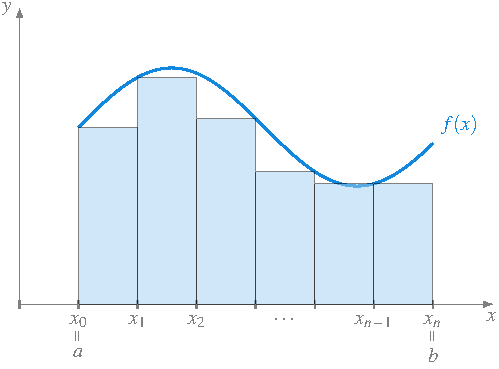
\includegraphics{img/integrales/suma-inferior-riemann.pdf}

}

\caption{Suma inferior de Riemann}

\end{figure}

\begin{definition}[Suma superior de
Riemann]\protect\hypertarget{def-suma-superior-riemann}{}\label{def-suma-superior-riemann}

Dada una función \(f: I\to\mathbb{R}\) acotada en el intervalo
\(I=[a,b]\) y una partición \(P=\{x_0, x_1, \ldots, x_n\}\) de \(I\), se
define la \emph{suma superior} de \(f\) respecto de \(P\), y se denota
\(S(f,P)\), como

\[
S(f,P) = \sum_{i=1}^n M_i(x_i-x_{i-1})
\]

donde \(M_i=\sup\{f(x): x\in[x_{i-1},x_i]\}\) para \(i=1,\ldots,n\).

\end{definition}

Gráficamente, si \(f\) es una función positiva, la suma superior se
puede interpretar como la suma de las areas de los rectángulos con base
\([x_{i-1},x_i]\) y altura \(M_i\).

\begin{figure}

{\centering 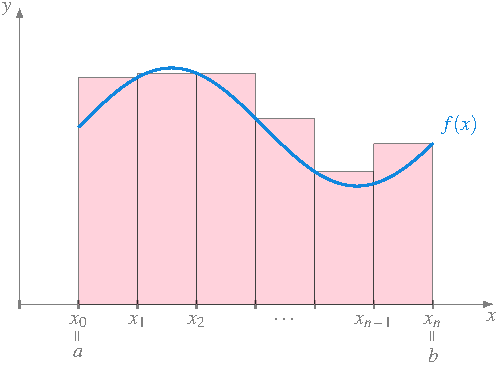
\includegraphics{img/integrales/suma-superior-riemann.pdf}

}

\caption{Suma inferior de Riemann}

\end{figure}

\begin{tcolorbox}[enhanced jigsaw, colback=white, colbacktitle=quarto-callout-warning-color!10!white, title=\textcolor{quarto-callout-warning-color}{\faExclamationTriangle}\hspace{0.5em}{Advertencia}, rightrule=.15mm, coltitle=black, arc=.35mm, opacityback=0, colframe=quarto-callout-warning-color-frame, bottomtitle=1mm, titlerule=0mm, toptitle=1mm, bottomrule=.15mm, toprule=.15mm, breakable, opacitybacktitle=0.6, left=2mm, leftrule=.75mm]

Obsérvese que si una función es negativa en un intervalo \(I\), sus
sumas de Riemann son negativas, ya que las alturas de los rectángulos
son negativas.

\begin{figure}[H]

{\centering 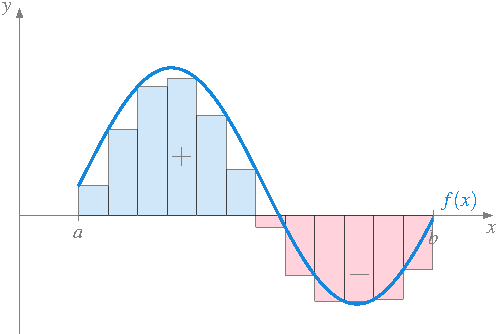
\includegraphics{img/integrales/sumas-riemann-positivas-negativas.pdf}

}

\caption{Sumas de Riemann de una función con valores positivos y
negativos en un intervalo.}

\end{figure}

\end{tcolorbox}

\href{https://www.geogebra.org/classic/nr6x8pjq}{
\includegraphics{img/logos/logo-geogebra.png}
Calculadora de sumas de Riemann}

\begin{proposition}[]\protect\hypertarget{prp-sumas-riemann-inferior-superior}{}\label{prp-sumas-riemann-inferior-superior}

Si \(f:I\to\mathbb{R}\) es una función acotada en el intervalo
\(I=[a,b]\) y \(P=\{x_0, x_1, \cdots, x_n\}\) es una partición de \(I\),
entonces \(s(f,P)\leq S(f,P)\).

\end{proposition}

\begin{tcolorbox}[enhanced jigsaw, colback=white, colbacktitle=quarto-callout-note-color!10!white, title=\textcolor{quarto-callout-note-color}{\faInfo}\hspace{0.5em}{Demostración}, rightrule=.15mm, coltitle=black, arc=.35mm, opacityback=0, colframe=quarto-callout-note-color-frame, bottomtitle=1mm, titlerule=0mm, toptitle=1mm, bottomrule=.15mm, toprule=.15mm, breakable, opacitybacktitle=0.6, left=2mm, leftrule=.75mm]

\begin{proof}

Para cada \(i=1,\ldots,n\) se tiene que

\[
m_i=\inf\{f(x): x\in[x_{i-1},x_i]\}\leq \sup\{f(x): x\in[x_{i-1},x_i]\} = M_i,
\]

de manera que

\[
s(f,P) = \sum_{i=1}^n m_i(x_i-x_{i-1}) \leq \sum_{i=1}^n M_i(x_i-x_{i-1}) = S(f,P),
\]

ya que \((x_i-x_{i-1})>0\) \(\forall i=1,\ldots,n\).

\end{proof}

\end{tcolorbox}

\begin{definition}[Refinamiento de una
partición]\protect\hypertarget{def-refinamiento-particion}{}\label{def-refinamiento-particion}

Dadas dos particiones \(P=\{x_0, x_1, \ldots, x_n\}\) y
\(Q=\{y_0, y_1, \ldots, y_m\}\) de un intervalo \(I=[a,b]\), se dice que
\(Q\) es un refinamiento de \(P\) si todos los puntos de \(P\) están en
\(Q\), es decir, \(P\subseteq Q\).

\end{definition}

\begin{proposition}[]\protect\hypertarget{prp-sumas-riemann-refinamiento}{}\label{prp-sumas-riemann-refinamiento}

Si \(f:I\to\mathbb{R}\) es una función acotada en el intervalo
\(I=[a,b]\), \(P\) es una partición de \(I\) y \(Q\) es un refinamiento
de \(P\), entonces

\begin{enumerate}
\def\labelenumi{\alph{enumi}.}
\tightlist
\item
  \(s(f,P)\leq S(f,Q)\)
\item
  \(s(f,Q)\leq S(f,P)\)
\end{enumerate}

\end{proposition}

\begin{tcolorbox}[enhanced jigsaw, colback=white, colbacktitle=quarto-callout-note-color!10!white, title=\textcolor{quarto-callout-note-color}{\faInfo}\hspace{0.5em}{Demostración}, rightrule=.15mm, coltitle=black, arc=.35mm, opacityback=0, colframe=quarto-callout-note-color-frame, bottomtitle=1mm, titlerule=0mm, toptitle=1mm, bottomrule=.15mm, toprule=.15mm, breakable, opacitybacktitle=0.6, left=2mm, leftrule=.75mm]

\begin{proof}

Veremos solo la prueba para las sumas inferiores.

\begin{enumerate}
\def\labelenumi{\alph{enumi}.}
\item
  Probaremos primero el resultado para un refinamiento con un punto más.
  Sea \(P=\{x_0, x_1, \cdots, x_n\}\) y supongamos que \(Q\) solo tiene
  un punto \(c\) más que \(P\). Sea \(k\in\{1,\ldots,n\}\) tal que
  \(c\in[x_{k-1},x_k]\) y tomemos \(m_k'=\inf\{f(x): x\in[x_{k-1},c]\}\)
  y \(m_k''=\inf\{f(x): x\in[c,x_k]\}\). Como
  \(m_k=\inf\{f(x): x\in[x_{k-1},x_k]\}\) resulta evidente que
  \(m_k\leq m_k'\) y \(m_k\leq m_k''\), por lo que

  \[
   m_k(x_k-x_{k-1}) = m_k(x_k-c)+m_k(c-x_{k-1})\leq m_k''(x_k-c)+m_k'(c-x_{k-1})
   \]

  y entonces

  \begin{align*}
   s(f,P) &= \sum_{i=1}^n m_i(x_i-x_{i-1}) = \sum_{i=1,i\neq k}^n m_i(x_i-x_{i-1}) + m_k(x_k-x_{k-1}) \\ &\leq \sum_{i=1,i\neq k}^n m_i(x_i-x_{i-1}) + m_k''(x_k-c) + m_k'(c-x_{k-1}) = s(f,Q).
   \end{align*}

  Para probar el caso general, si \(Q\) es un refinamiento cualquiera de
  \(P\), entonces existe una sucesión finita de particiones de \(I\),
  \(P_1,P_2,\ldots,P_r\) tales que
  \(P=P_1\subset P_2\subset\cdots \subset P_r=Q\) y cada \(P_i\) tiene
  solo un punto más que \(P_{i-1}\). Así pues, por el resultado
  anterior,

  \[
   s(f,P)\leq s(f,P_2)\leq \cdots \leq s(f,Q).
   \]
\item
  La prueba para las sumas superiores es análoga y se deja como
  ejercicio.
\end{enumerate}

\end{proof}

\end{tcolorbox}

\begin{proposition}[]\protect\hypertarget{prp-sumas-riemann-particiones}{}\label{prp-sumas-riemann-particiones}

Si \(f:I\to\mathbb{R}\) es una función acotada en el intervalo
\(I=[a,b]\) y \(P\) y \(Q\) son dos particiones de \(I\), entonces
\(s(f,P)\leq S(f,Q)\) y \(s(f,Q)\leq S(f,P)\).

\end{proposition}

\begin{tcolorbox}[enhanced jigsaw, colback=white, colbacktitle=quarto-callout-note-color!10!white, title=\textcolor{quarto-callout-note-color}{\faInfo}\hspace{0.5em}{Demostración}, rightrule=.15mm, coltitle=black, arc=.35mm, opacityback=0, colframe=quarto-callout-note-color-frame, bottomtitle=1mm, titlerule=0mm, toptitle=1mm, bottomrule=.15mm, toprule=.15mm, breakable, opacitybacktitle=0.6, left=2mm, leftrule=.75mm]

\begin{proof}

Tomando la partición de \(I\) \(P'=P\cup Q\), se tiene que \(P'\) es un
refinamiento de \(P\) y \(Q\), de manera que, según las proposiciones
anteriores se tiene

\[
s(f,P)\leq s(f,P')\leq S(f,P')\leq S(f,Q)
\]

y

\[
s(f,Q)\leq s(f,P')\leq S(f,P')\leq S(f,P).
\]

\end{proof}

\end{tcolorbox}

\hypertarget{integrales-de-riemann}{%
\section{Integrales de Riemann}\label{integrales-de-riemann}}

Como acabamos de ver, dada una función \(f\) positiva en un intervalo
\(I\), para cualquier partición \(P\) de \(I\), la suma inferior de
Riemann es una aproximación por defecto del área encerrada entre la
gráfica de \(f\) y el eje \(x\) en el intervalo \(I\), mientras que la
suma superior de Riemann es una aproximación por exceso. Si al hacer
refinamientos de la partición \(P\), cada vez con un mayor número de
subintervalos, las sumas inferiores crecen y las superiores decrecen, se
obtienen aproximaciones cada vez mejores. Podemos explotar esta idea
para calcular el area área encerrada entre la gráfica de \(f\) y el eje
\(x\) tomando particiones con subintervalos cada vez más pequeños.

\begin{definition}[Integral inferior de
Riemann]\protect\hypertarget{def-integral-inferior-riemann}{}\label{def-integral-inferior-riemann}

Dada una función \(f:I\to\mathbb{R}\) acotada en el intervalo
\(I=[a,b]\), se define la \emph{integral inferior} de \(f\) en \(I\)
como el número
\(\underline{\int_a^b} f =\sup\{s(f,P): P\in \mathcal{P}(I)\}\).

\end{definition}

\begin{definition}[Integral superior de
Riemann]\protect\hypertarget{def-integral-superior-riemann}{}\label{def-integral-superior-riemann}

Dada una función \(f:I\to\mathbb{R}\) acotada en el intervalo
\(I=[a,b]\), se define la \emph{integral superior} de \(f\) en \(I\)
como el número
\(\overline{\int_a^b} f =\inf\{S(f,P): P\in \mathcal{P}(I)\}\).

\end{definition}

\begin{proposition}[]\protect\hypertarget{prp-integral-riemann-inferior-superior}{}\label{prp-integral-riemann-inferior-superior}

Si \(f:I\to\mathbb{R}\) es una función acotada en el intervalo
\(I=[a,b]\), entonces
\(\underline{\int_a^b} f\leq \overline{\int_a^b}f\).

\end{proposition}

\begin{tcolorbox}[enhanced jigsaw, colback=white, colbacktitle=quarto-callout-note-color!10!white, title=\textcolor{quarto-callout-note-color}{\faInfo}\hspace{0.5em}{Demostración}, rightrule=.15mm, coltitle=black, arc=.35mm, opacityback=0, colframe=quarto-callout-note-color-frame, bottomtitle=1mm, titlerule=0mm, toptitle=1mm, bottomrule=.15mm, toprule=.15mm, breakable, opacitybacktitle=0.6, left=2mm, leftrule=.75mm]

\begin{proof}

Sean \(P\) y \(Q\) dos particiones cualesquiera de \(I\). Por la
proposición anterior, \(s(f,P)\leq S(f,Q)\)
\(\forall P\in\mathcal(P)(I)\), de modo que \(S(f,Q)\) es una cota
superior de todas las sumas inferiores, y por tanto,

\[
\underline{\int_a^b} f =  \sup\{s(f,P): P\in\mathcal{P}(I)\}\leq S(f,Q)
\]

Como esto es cierto para cualquier partición \(Q\), se tiene que
\(\underline{\int_a^b} f\) es una cota inferior de todas las sumas
superiores, y por tanto,

\[
\underline{\int_a^b} f \leq \inf\{S(f,Q): Q\in\mathcal{P}(I)\} = \overline{\int_a^b}f.
\]

\end{proof}

\end{tcolorbox}

\begin{definition}[Integral de
Riemann]\protect\hypertarget{def-integral-riemann}{}\label{def-integral-riemann}

Dada una función \(f:I\to\mathbb{R}\) acotada en el intervalo
\(I=[a,b]\), se dice que \(f\) es \emph{integrable Riemann} en \(I\) si

\[
\underline{\int_a^b} f = \overline{\int_a^b}f,
\]

y a este valor se le llama \emph{integral de Riemann} o \emph{integral
definida} de \(f\) en \(I\) y se denota por \(\int_a^b f\), o bien

\[
\int_a^b f(x)\,dx
\]

\end{definition}

\begin{tcolorbox}[enhanced jigsaw, colback=white, colbacktitle=quarto-callout-note-color!10!white, title=\textcolor{quarto-callout-note-color}{\faInfo}\hspace{0.5em}{Nota}, rightrule=.15mm, coltitle=black, arc=.35mm, opacityback=0, colframe=quarto-callout-note-color-frame, bottomtitle=1mm, titlerule=0mm, toptitle=1mm, bottomrule=.15mm, toprule=.15mm, breakable, opacitybacktitle=0.6, left=2mm, leftrule=.75mm]

Si \(f\) es integrable Riemann en \(I\), el número \(\int_a^b f(x)\,dx\)
es el único número real que verifica
\(s(f,P)\leq \int_a^b f(x)\,dx\leq S(f,P)\)
\(\forall P\in\mathcal{P}(I)\).

\end{tcolorbox}

En ocasiones, omitiremos el ``de Riemann'' para referirnos a una
integral de Riemann y simplemente se escribirá integral, cuando en el
contexto esté claro que se trata de la integral de Riemann.

\begin{example}[]\protect\hypertarget{exm-sumas-riemann}{}\label{exm-sumas-riemann}

~

\begin{enumerate}
\def\labelenumi{\alph{enumi}.}
\item
  Veamos que si \(f(x)=c\), es una función constante en \(I=[a,b]\),
  entonces \(f\) es integrable en \(I\).

  Sea \(P=\{x_0, x_1, \ldots, x_n\}\) una partición de \([a,b]\),
  entonces

  \begin{align*}
   s(f,P) &= \sum_{i=1}^n m_i(x_i-x_{i-1}) = \sum_{i=1}^n c(x_i-x_{i-1}) \\ 
   &= c\sum_{i=1}^n (x_i-x_{i-1}) = c(x_n-x_0) = c(b-a).
   \end{align*}

  Del mismo modo,

  \begin{align*}
   S(f,P) &= \sum_{i=1}^n M_i(x_i-x_{i-1}) = \sum_{i=1}^n c(x_i-x_{i-1})\\ 
   & = c\sum_{i=1}^n (x_i-x_{i-1}) = c(x_n-x_0) = c(b-a).
   \end{align*}

  Así pues, \(s(f,P) = S(f,P)=c(b-a)\) \(\forall P\in\mathcal{P}(I)\) y
  \(\int_a^b f(x)\,dx = c(b-a)\).
\item
  Veamos que \(f(x)=x\) es integrable en \([0,1]\).

  Sea \(P_n=\{0, \frac{1}{n}, \frac{2}{n}, \ldots, \frac{n}{n}\}\) una
  partición de \([0,1]\). Vamos a probar primero que
  \(\sup\{s(f,P_n):n\in\mathbb{N}\} = \inf\{S(f,P_n):n\in\mathbb{N}\}\).
  Como \(f\) es creciente y continua en \([0,1]\), se cumple que

  \begin{align*}
   m_i &= \inf\{f(x): x\in[x_{i-1},x_i]\} = f(x_{i-1}),\\ 
   M_i &= \sup\{f(x): x\in[x_{i-1},x_i]\} = f(x_i),
   \end{align*}

  y por tanto,

  \begin{align*}
   s(f,P_n) &= \sum_{i=1}^n m_i\left(\frac{i}{n}-\frac{i-1}{n}\right) = \sum_{i=1}^n f\left(\frac{i-1}{n}\right)\frac{1}{n} = \sum_{i=1}^n \frac{i-1}{n}\frac{1}{n}\\
   & = \frac{1}{n^2}\sum_{i=1}^n (i-1) =\frac{1}{n^2}\frac{(n-1)n}{2} = \frac{1}{2}\left(1-\frac{1}{n}\right),\\
   S(f,P_n) &= \sum_{i=1}^n M_i\left(\frac{i}{n}-\frac{i-1}{n}\right) = \sum_{i=1}^n f\left(\frac{i}{n}\right)\frac{1}{n} = \sum_{i=1}^n \frac{i}{n}\frac{1}{n}\\
   & = \frac{1}{n^2}\sum_{i=1}^n i =\frac{1}{n^2}\frac{n(n+1)}{2} = \frac{1}{2}\left(1+\frac{1}{n}\right).\\
   \end{align*}

  Así pues,

  \[
   \begin{gathered}
   \sup\{s(f,P_n):n\in\mathbb{N}\} = \sup\left\{\frac{1}{2}\left(1-\frac{1}{n}\right):n\in\mathbb{N}\right\} =\frac{1}{2} \\ 
   = \inf\left\{\frac{1}{2}\left(1+\frac{1}{n}\right):n\in\mathbb{N}\right\} = \inf\{S(f,P_n):n\in\mathbb{N}\}
   \end{gathered}
   \]

  Ahora bien, como

  \[
   \begin{gathered}
   \sup\{s(f,P_n):n\in\mathbb{N}\}\leq \sup\{s(f,P):P\in\mathcal{P}(I)\} = \underline{\int_0^1} f \\
   \leq \overline{\int_0^1} f =\inf\{S(f,P):P\in\mathcal{P}(I)\} \leq \inf\{S(f,P_n):n\in\mathbb{N}\}
   \end{gathered}
   \]

  se puede concluir que
  \(\underline{\int_0^1} f = \overline{\int_0^1} f\), y por tanto
  \(\int_0^1 f(x)\, dx = \frac{1}{2}\).
\end{enumerate}

\end{example}

\begin{example}[]\protect\hypertarget{exm-funcion-no-integrable-riemann}{}\label{exm-funcion-no-integrable-riemann}

La función

\[
f(x) = 
\begin{cases}
1 & \mbox{si } x\in\mathbb{Q}\cap[0,1]\\
0 & \mbox{si } x\in\mathbb{R}\setminus\mathbb{Q}\cap[0,1]
\end{cases}
\]

no es integrable Riemann ya que para cualquier partición
\(P=\{x_0, x_1, \ldots, x_n\}\) del intervalo \([0,1]\) se tiene que

\begin{align*}
m_i &= \inf\{f(x): x\in [x_{i-1},x_i]\} = 0,\\
M_i &= \sup\{f(x): x\in [x_{i-1},x_i]\} = 1,
\end{align*}

por lo que \(s(f,P)=0\) y \(S(f,P)=1\)
\(\forall P\in\mathcal{P}([0,1])\).

Así pues, \(\underline{\int_a^b}f = 0 \neq \overline{\int_a^b}f=1\).

\end{example}

\begin{theorem}[Criterio de integrabilidad de
Riemann]\protect\hypertarget{thm-criterio-integrabilidad-riemann}{}\label{thm-criterio-integrabilidad-riemann}

Una función \(f:I\to\mathbb{R}\) acotada en el intervalo \(I=[a,b]\) es
integrable en \(I\) si y sólo si para cada \(\varepsilon>0\) existe una
partición \(P\in\mathcal{P}(I)\) tal que \(S(f,P)-s(f,P)<\varepsilon\).

\end{theorem}

\begin{tcolorbox}[enhanced jigsaw, colback=white, colbacktitle=quarto-callout-note-color!10!white, title=\textcolor{quarto-callout-note-color}{\faInfo}\hspace{0.5em}{Demostración}, rightrule=.15mm, coltitle=black, arc=.35mm, opacityback=0, colframe=quarto-callout-note-color-frame, bottomtitle=1mm, titlerule=0mm, toptitle=1mm, bottomrule=.15mm, toprule=.15mm, breakable, opacitybacktitle=0.6, left=2mm, leftrule=.75mm]

\begin{proof}

Supongamos que \(f\) es integrable Riemann en \(I\), es decir,
\(\underline{\int_a^b}f = \overline{\int_a^b}f\). Dado \(\varepsilon>0\)
existe \(P_1\in\mathcal{P}(I)\) tal que
\(\underline{\int_a^b} f-\frac{\varepsilon}{2}\leq s(f,P_1)\) por ser
\(\underline{\int_a^b} f =\sup\{s(f,P): P\in \mathcal{P}(I)\}\).

Del mismo modo, por ser
\(\overline{\int_a^b} f =\inf\{S(f,P): P\in \mathcal{P}(I)\}\), existe
una partición \(P_2\in\mathcal{P}(I)\) tal que
\(\overline{\int_a^b} f+\frac{\varepsilon}{2} \geq S(f,P_2)\).

Tomando \(P = P_1\cup P_2\), se tiene que \(s(f,P_1)\leq s(f,P)\) y
\(S(f,P)\leq S(f,P_2)\). Así pues,

\[
S(f,P)-s(f,P) \leq S(f,P_2)-s(f,P_1) \leq \left(\overline{\int_a^b} f+\frac{\varepsilon}{2}\right) - \left(\underline{\int_a^b} f-\frac{\varepsilon}{2}\right) = \varepsilon.
\]

Para probar el otro sentido de la implicación, supongamos que para cada
\(\varepsilon>0\) existe una partición \(P\in\mathcal{P}(I)\) tal que
\(S(f,P)-s(f,P)<\varepsilon\). Entonces,

\[
0\leq \overline{\int_a^b} f- \underline{\int_a^b} f \leq S(f,P)-s(f,P)<\varepsilon,
\]

y como esto es cierto para cualquier \(\varepsilon>0\), se tiene
\(\overline{\int_a^b} f=\underline{\int_a^b} f\) y \(f\) es integrable
Riemann.

\end{proof}

\end{tcolorbox}

\begin{corollary}[]\protect\hypertarget{cor-criterio-integrabilidad-riemann}{}\label{cor-criterio-integrabilidad-riemann}

Dada una función \(f:I\to\mathbb{R}\) acotada en el intervalo
\(I=[a,b]\), si existe una sucesión de particiones
\((P_n)_{n=1}^\infty\) de \(I\) tal que
\(\lim_{n\to\infty} S(f,P_n)-s(f,P_n) =0\), entonces \(f\) es integrable
Riemann en \(I\) y

\[
\int_a^b f(x)\,dx = \lim_{n\to\infty} s(f,P_n) = \lim_{n\to\infty} S(f,P_n).
\]

\end{corollary}

\begin{tcolorbox}[enhanced jigsaw, colback=white, colbacktitle=quarto-callout-note-color!10!white, title=\textcolor{quarto-callout-note-color}{\faInfo}\hspace{0.5em}{Demostración}, rightrule=.15mm, coltitle=black, arc=.35mm, opacityback=0, colframe=quarto-callout-note-color-frame, bottomtitle=1mm, titlerule=0mm, toptitle=1mm, bottomrule=.15mm, toprule=.15mm, breakable, opacitybacktitle=0.6, left=2mm, leftrule=.75mm]

\begin{proof}

Dado \(\varepsilon>0\), como \(\lim_{n\to\infty} S(f,P_n)-s(f,P_n) =0\),
existe \(k\in\mathbb{N}\) tal que \(S(f,P_k)=s(f,P_k)<\varepsilon\),
luego, por el criterio de integrabilidad de Riemann, se tiene que \(f\)
es integrable en \(I\).

Para calcular el valor de la integral, se tiene

\[
\begin{gathered}
\lim_{n\to\infty} s(f,P_n) \leq \sup\{s(f,P):n\in\mathbb{N}\} \leq \sup\{s(f,P): P\in \mathcal{P}(I)\} = \int_a^b f(x)\, dx \\
= \inf\{S(f,P): P\in\mathcal{P}(I)\} \leq \inf\{S(f,P_n): n\in\mathbb{N}\} \leq \lim_{n\to\infty} S(f,P_n),
\end{gathered}
\]

y como \(\lim_{n\to\infty} s(f,P_n) = \lim_{n\to\infty} S(f,P_n)\), las
desigualdades anteriores se convierten en igualdades y por tanto,

\[
\int_a^b f(x)\,dx = \lim_{n\to\infty} s(f,P_n) = \lim_{n\to\infty} S(f,P_n).
\]

\end{proof}

\end{tcolorbox}

\begin{tcolorbox}[enhanced jigsaw, colback=white, colbacktitle=quarto-callout-important-color!10!white, title=\textcolor{quarto-callout-important-color}{\faExclamation}\hspace{0.5em}{Importante}, rightrule=.15mm, coltitle=black, arc=.35mm, opacityback=0, colframe=quarto-callout-important-color-frame, bottomtitle=1mm, titlerule=0mm, toptitle=1mm, bottomrule=.15mm, toprule=.15mm, breakable, opacitybacktitle=0.6, left=2mm, leftrule=.75mm]

Este último resultado nos permite calcular una integral como el límite
de las sumas de Riemann tomando una sucesión de particiones cada vez más
refinada.

\end{tcolorbox}

\hypertarget{propiedades-de-la-integral-de-riemann}{%
\section{Propiedades de la integral de
Riemann}\label{propiedades-de-la-integral-de-riemann}}

\begin{theorem}[]\protect\hypertarget{thm-linealidad-integral-riemann}{}\label{thm-linealidad-integral-riemann}

Si \(f,g:I\to\mathbb{R}\) son dos funciones integrables Riemann en
\(I=[a,b]\), entonces

\begin{enumerate}
\def\labelenumi{\alph{enumi}.}
\item
  \(f+g\) es integrable Riemann en \(I\) y
  \(\int_a^b (f+g)(x)\, dx = \int_a^b f(x)\,dx + \int_a^b g(x)\,dx.\)
\item
  Para cualquier \(c\in\mathbb{R}\), \(cf\) es integrable Riemann en
  \(I\) y \(\int_a^b cf(x)\, dx = c\int_a^b f(x)\,dx.\)
\end{enumerate}

\end{theorem}

\begin{tcolorbox}[enhanced jigsaw, colback=white, colbacktitle=quarto-callout-note-color!10!white, title=\textcolor{quarto-callout-note-color}{\faInfo}\hspace{0.5em}{Demostración}, rightrule=.15mm, coltitle=black, arc=.35mm, opacityback=0, colframe=quarto-callout-note-color-frame, bottomtitle=1mm, titlerule=0mm, toptitle=1mm, bottomrule=.15mm, toprule=.15mm, breakable, opacitybacktitle=0.6, left=2mm, leftrule=.75mm]

\begin{proof}

Veamos la demostración de cada apartado.

\begin{enumerate}
\def\labelenumi{\alph{enumi}.}
\item
  En primer lugar, resulta sencillo ver que para cualquier subintervalo
  \(J\) de \(I\) se cumple

  \begin{equation}\protect\hypertarget{eq-1}{}{
  \begin{gathered}
  \inf\{(f+g)(x): x\in J\} \geq \inf\{f(x): x\in J\} + \inf\{g(x): x\in J\}\\
  \sup\{(f+g)(x): x\in J\} \leq \sup\{f(x): x\in J\} + \sup\{g(x): x\in J\}
  \end{gathered}
  }\label{eq-1}\end{equation}

  Dado \(\varepsilon>0\), como \(f\) y \(g\) son integrables, existen
  dos particiones \(P_1,P_2\in \mathcal{P}(I)\) tales que

  \[
  \begin{gathered}
  S(f,P_1)-s(f,P_1)\leq \frac{\varepsilon}{2}\\
  S(g,P_2)-s(g,P_2)\leq \frac{\varepsilon}{2}
  \end{gathered}
  \]

  Tomando ahora el refinamiento \(P=P_1\cup P_2\) de \(P_1\) y \(P_2\) y
  la Ecuación~\ref{eq-1} se tiene

  \begin{align*}
  s(f+g,P) &\geq s(f,P) + s(g,P) \geq s(f,P_1) + s(g,P_2)\\
  S(f+g,P) &\leq S(f,P) + S(g,P) \leq S(f,P_1) + S(g,P_2)
  \end{align*}

  de manera que

  \begin{align*}
  S(f+g,P)-s(f+g,P) &\leq (S(f,P_1)+S(g,P_2))-(s(f,P_ 1)+s(g,P_2)) \\
  &\leq \frac{\varepsilon}{2}+\frac{\varepsilon}{2} =\varepsilon.
  \end{align*}

  Y, por tanto, \(f+g\) es integrable Riemann en \(I\).

  Además,

  \[
  s(f,P) + s(g,P) \leq s(f+g,P) \leq \int_a^b (f+g) \leq  S(f+g,P) \leq S(f,P) + S(g,P)
  \]

  y

  \[
  s(f,P) + s(g,P) \leq  \int_a^b f + \int_a^b g \leq S(f,P) + S(g,P),
  \]

  por lo que se tiene

  \[
  0\leq \left|\int_a^b (f+g) - \left(\int_a^b f + \int_a^b g\right)\right| \leq (S(f,P)+S(g,P)) - (s(f,P)+s(g,P)) \leq \varepsilon,
  \]

  y por consiguiente, \(\int_a^b (f+g) = \int_a^b f + \int_a^b g\).
\item
  Si \(c=0\) entonces \(cf=0\), y por tanto, \(cf\) es integrable y
  además \(\int_a^b cf = 0 = c\int_a^b f\).

  Supongamos ahora que \(c>0\). Resulta sencillo ver que para cualquier
  subintervalo \(J\) de \(I\) se cumple

  \begin{equation}\protect\hypertarget{eq-2}{}{
  \begin{gathered}
  \inf\{(cf)(x): x\in J\} = c\inf\{f(x): x\in J\}\\
  \sup\{(cf)(x): x\in J\} = c\sup\{f(x): x\in J\}
  \end{gathered}
  }\label{eq-2}\end{equation}

  de manera que si \(P\) es una partición de \(I\), entonces
  \(s(cf,P)= cs(f,P)\) y \(S(cf,P) = cS(f,P)\).

  Como \(f\) es integrable Riemann, dado \(\varepsilon>0\) existe una
  partición \(P\in\mathcal{P}(I)\) tal que
  \(S(f,P)-s(f,P)\leq \frac{\varepsilon}{c} >0\). Por otro lado, según
  la Ecuación~\ref{eq-2},

  \[
  S(cf,P) - s(cf,P) = c S(f,P) - cs(f,P) = c(S(f,P)-s(f,P)) < c\frac{\varepsilon}{c} = \varepsilon,
  \]

  de manera que \(cf\) es integrable en \(I\), y además,

  \begin{align*}
  \int_a^b cf &= \inf\{S(cf,P): P\in \mathcal{P}(I)\} = \inf\{cS(f,P): P\in \mathcal{P}(I)\} \\
  &= c\inf\{S(f,P): P\in \mathcal{P}(I)\} = c\int_a^b f.
  \end{align*}

  Finalmente, si \(c<0\), resulta sencillo ver que para cualquier
  subintervalo \(J\) de \(I\) se cumple

  \begin{equation}\protect\hypertarget{eq-3}{}{
  \begin{gathered}
  \inf\{(cf)(x): x\in J\} = c\sup\{f(x): x\in J\}\\
  \sup\{(cf)(x): x\in J\} = c\inf\{f(x): x\in J\}
  \end{gathered}
  }\label{eq-3}\end{equation}

  de manera que si \(P\) es una partición de \(I\), entonces
  \(s(cf,P)= cS(f,P)\) y \(S(cf,P) = cs(f,P)\).

  Como \(f\) es integrable Riemann, dado \(\varepsilon>0\) existe una
  partición \(P\in\mathcal{P}(I)\) tal que
  \(S(f,P)-s(f,P)\leq \frac{\varepsilon}{-c} >0\). Por otro lado, según
  la Ecuación~\ref{eq-3},

  \begin{align*}
  S(cf,P) - s(cf,P) &= c s(f,P) - cS(f,P) = c(s(f,P)-S(f,P)) \\
  &= c(S(f,P)-s(f,P)) < -c\frac{\varepsilon}{-c} = \varepsilon,
  \end{align*}

  de manera que \(cf\) es integrable en \(I\), y además,

  \begin{align*}
  \int_a^b cf &= \inf\{S(cf,P): P\in \mathcal{P}(I)\} = \inf\{cs(f,P): P\in \mathcal{P}(I)\} \\
  &= c\sup\{s(f,P): P\in \mathcal{P}(I)\} = c\int_a^b f.
  \end{align*}
\end{enumerate}

\end{proof}

\end{tcolorbox}

\begin{proposition}[]\protect\hypertarget{prp-integral-funcion-positiva}{}\label{prp-integral-funcion-positiva}

Si \(f:I\to\mathbb{R}\) es una función integrable Riemann en \(I=[a,b]\)
y \(f(x)\geq 0\) \(\forall x\in I\), entonces
\(\int_a^b f(x)\,dx \geq 0\).

\end{proposition}

\begin{tcolorbox}[enhanced jigsaw, colback=white, colbacktitle=quarto-callout-note-color!10!white, title=\textcolor{quarto-callout-note-color}{\faInfo}\hspace{0.5em}{Demostración}, rightrule=.15mm, coltitle=black, arc=.35mm, opacityback=0, colframe=quarto-callout-note-color-frame, bottomtitle=1mm, titlerule=0mm, toptitle=1mm, bottomrule=.15mm, toprule=.15mm, breakable, opacitybacktitle=0.6, left=2mm, leftrule=.75mm]

\begin{proof}

Para cualquier partición \(P\in\mathcal{P}(I)\) se tiene que \(f(x)\) es
positiva en cualquier intervalo de la partición y por tanto
\(s(f,P)\geq 0\). Así pues,
\(\int_a^b f(x)\,dx = \sup\{s(f,P):P\in \mathcal{P}(I)\}\geq 0\).

\end{proof}

\end{tcolorbox}

\begin{corollary}[]\protect\hypertarget{cor-integral-funcion-negativa}{}\label{cor-integral-funcion-negativa}

Si \(f:I\to\mathbb{R}\) es una función integrable Riemann en \(I=[a,b]\)
y \(f(x)\leq 0\) \(\forall x\in I\), entonces
\(\int_a^b f(x)\,dx \leq 0\).

\end{corollary}

\begin{tcolorbox}[enhanced jigsaw, colback=white, colbacktitle=quarto-callout-note-color!10!white, title=\textcolor{quarto-callout-note-color}{\faInfo}\hspace{0.5em}{Demostración}, rightrule=.15mm, coltitle=black, arc=.35mm, opacityback=0, colframe=quarto-callout-note-color-frame, bottomtitle=1mm, titlerule=0mm, toptitle=1mm, bottomrule=.15mm, toprule=.15mm, breakable, opacitybacktitle=0.6, left=2mm, leftrule=.75mm]

\begin{proof}

Consideremos la función \(-f(x)\geq 0\) \(\forall x\in\mathbb{R}\). Como
\(f\) es integrable en \(I\), también lo es \((-1)f\) y

\[
\int_a^b f(x)\, dx = \int_a^b (-1)(-f(x))\,dx = - \int_a^b -f(x)\,dx \leq 0,
\]

ya que por la proposición anterior \(\int_a^b -f(x)\,dx \geq 0\).

\end{proof}

\end{tcolorbox}

\begin{tcolorbox}[enhanced jigsaw, colback=white, colbacktitle=quarto-callout-caution-color!10!white, title=\textcolor{quarto-callout-caution-color}{\faFire}\hspace{0.5em}{Precaución}, rightrule=.15mm, coltitle=black, arc=.35mm, opacityback=0, colframe=quarto-callout-caution-color-frame, bottomtitle=1mm, titlerule=0mm, toptitle=1mm, bottomrule=.15mm, toprule=.15mm, breakable, opacitybacktitle=0.6, left=2mm, leftrule=.75mm]

Este resultado nos advierte de que no se puede utilizar directamente la
integral de Riemann para calcular el area entre la gráfica de la función
y el eje \(x\) si la función presenta valores negativos en el intervalo
de integración \(I\).

En estos casos, el recurso habitual para calcular el área es calcular la
integral del valor absoluto de la función.

\end{tcolorbox}

\begin{figure}

\begin{minipage}[t]{0.50\linewidth}

{\centering 

\raisebox{-\height}{

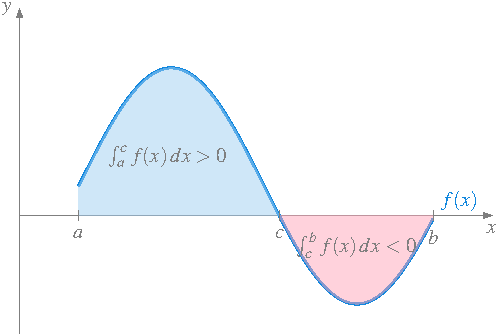
\includegraphics{img/integrales/area-funcion-positiva-negativa.pdf}

}

\caption{Integral de una función con valores positivos y negativos en un
intervalo \(I\)}

}

\end{minipage}%
%
\begin{minipage}[t]{0.50\linewidth}

{\centering 

\raisebox{-\height}{

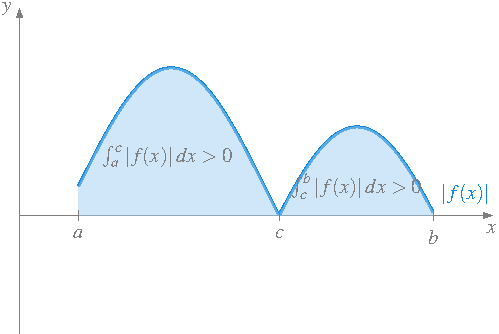
\includegraphics{img/integrales/integral-valor-absoluto.pdf}

}

\caption{Cálculo del area encerrada entre una función de una función y
el eje \(x\) mediante la integral del valor absoluto de la función.}

}

\end{minipage}%

\end{figure}

\begin{corollary}[]\protect\hypertarget{cor-integral-funcion-mayor-que-otra}{}\label{cor-integral-funcion-mayor-que-otra}

Si \(f,g:I\to\mathbb{R}\) son dos funciones integrables Riemann en
\(I=[a,b]\) y \(f(x)\leq g(x)\) \(\forall x\in I\), entonces
\(\int_a^b f(x)\,dx \leq \int_a^b g(x)\,dx\).

\end{corollary}

\begin{tcolorbox}[enhanced jigsaw, colback=white, colbacktitle=quarto-callout-note-color!10!white, title=\textcolor{quarto-callout-note-color}{\faInfo}\hspace{0.5em}{Demostración}, rightrule=.15mm, coltitle=black, arc=.35mm, opacityback=0, colframe=quarto-callout-note-color-frame, bottomtitle=1mm, titlerule=0mm, toptitle=1mm, bottomrule=.15mm, toprule=.15mm, breakable, opacitybacktitle=0.6, left=2mm, leftrule=.75mm]

\begin{proof}

Consideremos la función \(g(x)-f(x)\geq 0\) \(\forall x\in\mathbb{R}\).
Como \(f\) y \(g\) son integrables en \(I\), también lo es \(g-f\) y

\[
\int_a^b g(x)-f(x)\, dx = \int_a^b g(x)\,dx - \int_a^b f(x)\,dx \geq 0 \Rightarrow \int_a^b f(x)\,dx \leq \int_a^b g(x)\,dx.
\]

\end{proof}

\end{tcolorbox}

\begin{corollary}[]\protect\hypertarget{cor-integral-funcion-acotada}{}\label{cor-integral-funcion-acotada}

Si \(f:I\to\mathbb{R}\) es una función integrable Riemann en \(I=[a,b]\)
y \(m\leq f(x)\leq M\) \(\forall x\in I\), entonces
\(m(b-a)\leq \int_a^b f(x)\,dx \leq M(b-a)\).

\end{corollary}

\begin{tcolorbox}[enhanced jigsaw, colback=white, colbacktitle=quarto-callout-note-color!10!white, title=\textcolor{quarto-callout-note-color}{\faInfo}\hspace{0.5em}{Demostración}, rightrule=.15mm, coltitle=black, arc=.35mm, opacityback=0, colframe=quarto-callout-note-color-frame, bottomtitle=1mm, titlerule=0mm, toptitle=1mm, bottomrule=.15mm, toprule=.15mm, breakable, opacitybacktitle=0.6, left=2mm, leftrule=.75mm]

\begin{proof}

Por el corolario anterior se tiene
\(\int_a^b m\,dx \leq \int_a^b f(x)\,dx \leq \int_a^b M\,dx\).

Por otro lado, como \(\int_a^b m\,dx = m(b-a)\) y
\(\int_a^b M\,dx = M(b-a)\) por tratarse de funciones constantes,
sustituyendo en la desigualdad anterior se tiene

\[
m(b-a)\leq \int_a^b f(x)\,dx \leq M(b-a).
\]

\end{proof}

\end{tcolorbox}

\begin{theorem}[Aditividad de la integral respecto del intervalo de
integración]\protect\hypertarget{thm-aditividad-integral-intervalo}{}\label{thm-aditividad-integral-intervalo}

Si \(f:I\to\mathbb{R}\) es una función acotada en \(I=[a,b]\) y
\(c\in(a,b)\), entonces \(f\) es integrable Riemann en \(I\) si y sólo
si \(f\) es integrable Riemann en \([a,c]\) y \([c,b]\). Además, en este
caso,

\[
\int_a^b f(x)\,dx = \int_a^c f(x)\,dx + \int_c^b f(x)\,dx
\]

\end{theorem}

\begin{tcolorbox}[enhanced jigsaw, colback=white, colbacktitle=quarto-callout-note-color!10!white, title=\textcolor{quarto-callout-note-color}{\faInfo}\hspace{0.5em}{Demostración}, rightrule=.15mm, coltitle=black, arc=.35mm, opacityback=0, colframe=quarto-callout-note-color-frame, bottomtitle=1mm, titlerule=0mm, toptitle=1mm, bottomrule=.15mm, toprule=.15mm, breakable, opacitybacktitle=0.6, left=2mm, leftrule=.75mm]

\begin{proof}

Supongamos que \(f\) es integrable en \(I\). Entonces, dado
\(\varepsilon>0\), existe \(P\in\mathcal{P}(I)\) tal que
\(S(f,P)-s(f,P)<\varepsilon\).

Sea \(Q=P\cup\{c\}\in\mathcal{P}(I)\). Como \(Q\) es un refinamiento de
\(P\), se cumple

\[
S(f,Q)-s(f,Q) \leq S(f,P)-s(f,P) \leq \varepsilon
\]

Tomando ahora las subparticiones \(Q_1=\{t\in Q:t\leq c\}\) y
\(Q_2=\{t\in Q: t\geq c\}\), se tiene que

\[
\begin{gathered}
(S(f,Q_1)-s(f,Q_1)) + (S(f,Q_2)-s(f,Q_2)) \\
= (S(f,Q_1) + S(f,Q_2)) - (s(f,Q_1) + s(f,Q_2)) \\
= S(f,P) - s(f,P) \leq S(f,Q) - s(f,Q) < \varepsilon,
\end{gathered}
\]

de manera que \(S(f,Q_1)-s(f,Q_1)<\varepsilon\) y
\(S(f,Q_2)-s(f,Q_2)<\varepsilon\), y por tanto, \(f\) es integrable en
\([a,c]\) y en \([c,b]\). Además,

\[
s(f,Q) = s(f,Q_1) + s(f,Q_2) \leq \int_a^c f + \int_c^b f \leq S(f,Q_1) + S(f,Q_2) = S(f,Q)
\]

para cualquier \(Q\in\mathcal{P}(I)\) y \(c\in Q\). Si
\(P\in\mathcal{P}(I)\), tomando \(Q=P\cup \{c\}\), \(Q\) es un
refinamiento de \(P\), y por tanto,

\[
\begin{gathered}
s(f,P) \leq s(f,Q) = s(f,Q_1) + s(f,Q_2) \leq \int_a^c f + \int_c^b f \\
\leq S(f,Q_1) + S(f,Q_2) = S(f,Q) \leq S(f,P),
\end{gathered}
\]

por lo que se concluye que \(\int_a^b f = \int_a^c f + \int_c^b f\).

Para probar el otro sentido de la implicación, supongamos que \(f\) es
integrable en \([a,c]\) y \([c,b]\). Dado \(\varepsilon>0\) existe
\(P_1\in\mathcal{P}([a,c])\) tal que
\(S(f,P_1)-s(f,P_1)<\frac{\varepsilon}{2}\) y existe
\(P_2\in\mathcal{P}([c,b])\) tal que
\(S(f,P_2)-s(f,P_2)<\frac{\varepsilon}{2}\).

Tomando ahora \(P=P_1\cup P_2\in \mathcal{P}(I)\), se cumple

\[
S(f,P)-s(f,P) = s(f,P_1) + S(f,P_2) - (s(f,P_1) + s(f,P_2)) < \frac{\varepsilon}{2}+\frac{\varepsilon}{2} =\varepsilon,
\]

por lo que \(f\) es integrable en \(I\).

\end{proof}

\end{tcolorbox}

A pesar de que la demostración es bastante larga, cuando \(f\) es
positiva, es obvio que el área entre la gráfica de \(f\) y el eje \(x\)
en el intervalo \([a,b]\) puede descomponerse en la suma de las áreas en
los intervalos \([a,c]\) y \([c,b]\) para cualquier \(c\in(a,b)\).

\begin{figure}

{\centering 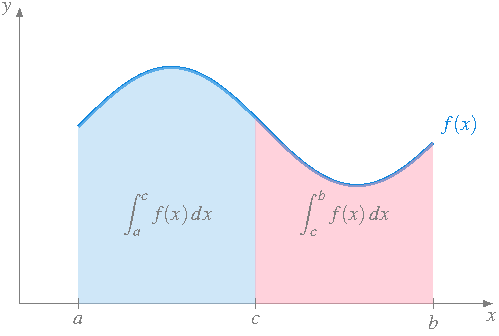
\includegraphics{img/integrales/aditividad-integral.pdf}

}

\caption{Aditividad de la integral respecto del intervalo de
integración}

\end{figure}

\hypertarget{clase-de-las-funciones-integrables}{%
\section{Clase de las funciones
integrables}\label{clase-de-las-funciones-integrables}}

A continuación trataremos de estudiar qué tipo de funciones son
integrables.

\begin{theorem}[]\protect\hypertarget{thm-integrabilidad-funciones-monótonas}{}\label{thm-integrabilidad-funciones-monótonas}

Si \(f:I\to\mathbb{R}\) es una función acotada y monótona en
\(I=[a,b]\), entonces \(f\) es integrable en \(I\).

\end{theorem}

\begin{tcolorbox}[enhanced jigsaw, colback=white, colbacktitle=quarto-callout-note-color!10!white, title=\textcolor{quarto-callout-note-color}{\faInfo}\hspace{0.5em}{Demostración}, rightrule=.15mm, coltitle=black, arc=.35mm, opacityback=0, colframe=quarto-callout-note-color-frame, bottomtitle=1mm, titlerule=0mm, toptitle=1mm, bottomrule=.15mm, toprule=.15mm, breakable, opacitybacktitle=0.6, left=2mm, leftrule=.75mm]

\begin{proof}

Supongamos que \(f\) es creciente en \(I\). Dado \(\varepsilon>0\)
existe un \(n\in\mathbb{N}\) tal que

\[
\frac{(f(b)-f(a))(b-a)}{n} < \varepsilon.
\]

Sea ahora \(P_n\in\mathcal{P}(I)\) la partición que divide \(I\) en
\(n\) subintervalos de igual longitud, es decir,
\(P=\{x_0, x_1, \ldots, x_n\}\) con \(x_i = a+\frac{(b-a)i}{n}\).

Como \(f\) es creciente en \(I\) se tiene

\begin{align*}
m_i &= \inf\{f(x): x\in[x_{i-1},x_i]\} = f(x_{i-1})\\
M_i &= \sup\{f(x): x\in[x_{i-1},x_i]\} = f(x_{i})
\end{align*} para \(i=1,\ldots,n\), de manera que

\begin{align*}
S(f,P_n)-s(f,P_n) &= \sum_{i=1}^n f(x_i)(x_i-x_{i-1}) - \sum_{i=1}^n f(x_{i-1})(x_i-x_{i-1}) \\
&= \sum_{i=1}^n (f(x_i)-f(x_{i-1}))\frac{b-a}{n} \\
&= \frac{b-1}{n}(f(x_1)-f(x_0))+(f(x_2)-f(x_1))+ \cdots \\ 
& \cdots + (f(x_{n-1})-f(x_{n-2})+ (f(x_n)-f(x_{n-1}))) \\
&= \frac{b-a}{n}(f(b)-f(a)) < \varepsilon.
\end{align*}

Así pues, \(f\) es integrable en \(I\).

\end{proof}

\end{tcolorbox}

\begin{theorem}[]\protect\hypertarget{thm-integrabilidad-funciones-continuas}{}\label{thm-integrabilidad-funciones-continuas}

Si \(f:I\to\mathbb{R}\) es una función continua en \(I=[a,b]\), entonces
\(f\) es integrable en \(I\).

\end{theorem}

\begin{tcolorbox}[enhanced jigsaw, colback=white, colbacktitle=quarto-callout-note-color!10!white, title=\textcolor{quarto-callout-note-color}{\faInfo}\hspace{0.5em}{Demostración}, rightrule=.15mm, coltitle=black, arc=.35mm, opacityback=0, colframe=quarto-callout-note-color-frame, bottomtitle=1mm, titlerule=0mm, toptitle=1mm, bottomrule=.15mm, toprule=.15mm, breakable, opacitybacktitle=0.6, left=2mm, leftrule=.75mm]

\begin{proof}

Observemos primero que como \(f\) es continua en \(I\), entonces es
uniformemente continua en \(I\) al ser \(I\) un intervalo cerrado.

Dado \(\varepsilon>0\), como \(f\) es uniformemente continua en \(I\),
para \(\varepsilon'=\frac{\varepsilon}{b-a}>0\) existe \(\delta>0\) tal
que si \(|x-y|<\delta\) entonces \(|f(x)-f(y)|<\varepsilon'\).

Sea \(P=\{x_0,x_1,\ldots,x_n\}\) una partición que divide \(I\) en
subintervalos de longitud menor que \(\delta\). Entonces, para cad
\(i=1,\ldots, n\) se tiene

\[
M_i-m_i = \sup\{|f(x)-f(y)|: x,y\in[x_{i-1},x_i]\} \leq \varepsilon',
\]

y por tanto,

\begin{align*}
S(f,P)-s(f,P) &= \sum_{i=1}^n M_i(x_i-x_{i-1}) - \sum_{i=1}^n m_i(x_i-x_{i-1}) \\
&= \sum_{i=1}^n (M_i-m_i)(x_i-x_{i-1})\\
& < \varepsilon' \sum_{i=1}^n (x_i-x_{i-1}) = \varepsilon' (b-a)  = \varepsilon.
\end{align*}

\end{proof}

\end{tcolorbox}

\begin{theorem}[]\protect\hypertarget{thm-integrabilidad-funciones-discontinuas}{}\label{thm-integrabilidad-funciones-discontinuas}

Si \(f:I\to\mathbb{R}\) es una función continua en \(I=[a,b]\), salvo en
un punto \(c\in I\), entonces \(f\) es integrable en \(I\).

\end{theorem}

\begin{tcolorbox}[enhanced jigsaw, colback=white, colbacktitle=quarto-callout-note-color!10!white, title=\textcolor{quarto-callout-note-color}{\faInfo}\hspace{0.5em}{Demostración}, rightrule=.15mm, coltitle=black, arc=.35mm, opacityback=0, colframe=quarto-callout-note-color-frame, bottomtitle=1mm, titlerule=0mm, toptitle=1mm, bottomrule=.15mm, toprule=.15mm, breakable, opacitybacktitle=0.6, left=2mm, leftrule=.75mm]

\begin{proof}

Se deja como ejercicio.

\end{proof}

\end{tcolorbox}

\begin{corollary}[]\protect\hypertarget{cor-integrabilidad-funciones-discontinuas}{}\label{cor-integrabilidad-funciones-discontinuas}

Si \(f:I\to\mathbb{R}\) es una función continua en \(I=[a,b]\), salvo en
un conjunto finito de puntos de \(I\), entonces \(f\) es integrable en
\(I\).

\end{corollary}

\begin{tcolorbox}[enhanced jigsaw, colback=white, colbacktitle=quarto-callout-note-color!10!white, title=\textcolor{quarto-callout-note-color}{\faInfo}\hspace{0.5em}{Demostración}, rightrule=.15mm, coltitle=black, arc=.35mm, opacityback=0, colframe=quarto-callout-note-color-frame, bottomtitle=1mm, titlerule=0mm, toptitle=1mm, bottomrule=.15mm, toprule=.15mm, breakable, opacitybacktitle=0.6, left=2mm, leftrule=.75mm]

\begin{proof}

Haremos la prueba por inducción sobre el número de puntos de
discontinuidad.

El caso para un solo punto de discontinuidad se ha probado en el teorema
anterior. Supongamos que si \(f\) tiene \(n\) puntos de discontinuidad
en \(I\) entonces es integrable Riemann en \(I\), y supongamos ahora que
\(f\) tiene \(n+1\) puntos de discontinuidad. Sea \(c\) el mayor de los
puntos de discontinuidad. Tomando \(\delta>0\) se tiene que \(f\) tiene
\(n\) puntos de discontinuidad en el intervalo \([a, c-\delta]\), por lo
que es integrable en este intervalo.

Sea ahora \(\varepsilon>0\). Como \(f\) es integrable en
\([a,c-\delta]\) existe una partición \(P_1\) de \([a,c-\delta]\) tal
que \(S(f,P_1)-s(f,P_2)<\frac{\varepsilon}{2}\). Por otro lado, \(f\)
está acotada en el intervalo \([c-\delta, b]\) y solo tiene una
discontinuidad, por el teorema anterior, \(f\) es integrable en
\([c-\delta,b]\), por lo que existe otra partición \(P_2\) de
\([c-\delta,b]\) tal que \(S(f,P_2)-s(f,P_2)<\frac{\varepsilon}{2}\).

Tomando la partición \(P=P_1\cup P_2\) que es un refinamiento de \(P_1\)
y \(P_2\), se tiene

\[
S(f,P)-s(f,P)\leq S(f,P_1)+S(f,P_2)-s(f,P_1)-s(f,P_2) < \frac{\varepsilon}{2}+\frac{\varepsilon}{2} = \varepsilon.
\]

Por consiguiente \(f\) es integrable Riemann con \(n+1\)
discontinuidades, y aplicando el principio de inducción queda probado el
resultado.

\end{proof}

\end{tcolorbox}

\begin{theorem}[]\protect\hypertarget{thm-integrabilidad-composicion-funciones}{}\label{thm-integrabilidad-composicion-funciones}

Si \(f:I\to\mathbb{R}\) es una función integrable en \(I=[a,b]\) y
\(g:J\to\mathbb{R}\) es una función continua en \(J=[c,d]\) con
\(f(I)\subseteq J\), entonces \(g\circ f\) es integrable en \(I\).

\end{theorem}

\begin{tcolorbox}[enhanced jigsaw, colback=white, colbacktitle=quarto-callout-note-color!10!white, title=\textcolor{quarto-callout-note-color}{\faInfo}\hspace{0.5em}{Demostración}, rightrule=.15mm, coltitle=black, arc=.35mm, opacityback=0, colframe=quarto-callout-note-color-frame, bottomtitle=1mm, titlerule=0mm, toptitle=1mm, bottomrule=.15mm, toprule=.15mm, breakable, opacitybacktitle=0.6, left=2mm, leftrule=.75mm]

\begin{proof}

Como \(g\) es continua en \(J\), está acotada en \(J\), de manera que
podemos tomar \(k>\sup\{g(x):x\in J\}-\inf\{f(x):x\in J\}\).

Por otro lado, como \(J\) es cerrado, \(g\) es uniformemente continua en
\(J\) y dado \(\varepsilon>0\), existe \(\delta<\varepsilon\) tal que si
\(|x-y|<\delta\) entonces \(|g(x)-g(y)|<\frac{\varepsilon}{2(b-a)}\).

Como \(f\) es integrable en \(I\) podemos tomar una partición
\(P=\{x_0,x_1,\ldots,x_n\}\) de \(I\), tal que

\[
S(f,P)-s(f,P) < \frac{\delta^2}{2k}.
\]

Para \(i=1,\ldots,n\), sea

\begin{align*}
m_i &= \inf\{f(x): x\in[x_{i-1},x_i]\}\\
M_i &= \sup\{f(x): x\in[x_{i-1},x_i]\}\\
m_i' &= \inf\{g\circ f(x): x\in[x_{i-1},x_i]\}\\
M_i' &= \sup\{g\circ f(x): x\in[x_{i-1},x_i]\}\\
\end{align*}

y sea

\begin{align*}
A &= \{i\in\{1,\ldots, n\}: M_i-m_i<\delta\}\\
B &= \{i\in\{1,\ldots, n\}: M_i-m_i\geq\delta\}
\end{align*}

Entonces se cumple que

\[
\delta\sum_{i\in B} (x_i-x_{i-1}) \leq \sum_{i\in B} (M_i-m_i)(x_i-x_{i-1}) \leq \sum_{i=1}^n (M_i-m_i)(x_i-x_{i-1}) < \frac{\delta^2}{2k}
\]

de donde se deduce que

\[
\sum_{i\in B} (x_i-x_{i-1}) < \frac{\delta}{2k}.
\]

Y utilizando los resultados anteriores se tiene

\begin{align*}
S(g\circ f,P)-s(g\circ f,P) &= \sum_{i\in A}(M_i'-m_i')(x_i-x_{i-1}) + \sum_{i\in B}(M_i'-m_i')(x_i-x_{i-1}) \\
&< \frac{\varepsilon}{2(b-a)} \sum_{i\in A}(x_i-x_{i-1}) + k \sum_{i\in B}(x_i-x_{i-1})\\
&< \frac{\varepsilon}{2}+\frac{\delta}{2} < \frac{\varepsilon}{2} + \frac{\varepsilon}{2} < \varepsilon,
\end{align*}

por lo que \(g\circ f\) es integrable en \(I\).

\end{proof}

\end{tcolorbox}

\begin{corollary}[]\protect\hypertarget{cor-integrabilidad-valor-absoluto}{}\label{cor-integrabilidad-valor-absoluto}

Si \(f:I\to\mathbb{R}\) es una función integrable en \(I=[a,b]\),
entonces la función \(|f|\) es integrable en \(I\).

\end{corollary}

\begin{tcolorbox}[enhanced jigsaw, colback=white, colbacktitle=quarto-callout-note-color!10!white, title=\textcolor{quarto-callout-note-color}{\faInfo}\hspace{0.5em}{Demostración}, rightrule=.15mm, coltitle=black, arc=.35mm, opacityback=0, colframe=quarto-callout-note-color-frame, bottomtitle=1mm, titlerule=0mm, toptitle=1mm, bottomrule=.15mm, toprule=.15mm, breakable, opacitybacktitle=0.6, left=2mm, leftrule=.75mm]

\begin{proof}

Como \(f\) es integrable en \(I\), \(f\) está acotada en \(I\), así que,
tomando \(c=\sup\{|f(x)|: x\in I\}\), basta aplicar el teorema anterior
con \(g=|x|\) en el intervalo \(J=[-c,c]\).

\end{proof}

\end{tcolorbox}

\begin{corollary}[]\protect\hypertarget{cor-integrabilidad-potencias}{}\label{cor-integrabilidad-potencias}

Si \(f:I\to\mathbb{R}\) es una función integrable en \(I=[a,b]\),
entonces la función \(f^n\) es integrable en \(I\) para cualquier
\(n\in\mathbb{N}\).

\end{corollary}

\begin{tcolorbox}[enhanced jigsaw, colback=white, colbacktitle=quarto-callout-note-color!10!white, title=\textcolor{quarto-callout-note-color}{\faInfo}\hspace{0.5em}{Demostración}, rightrule=.15mm, coltitle=black, arc=.35mm, opacityback=0, colframe=quarto-callout-note-color-frame, bottomtitle=1mm, titlerule=0mm, toptitle=1mm, bottomrule=.15mm, toprule=.15mm, breakable, opacitybacktitle=0.6, left=2mm, leftrule=.75mm]

\begin{proof}

Como \(f\) es integrable en \(I\), \(f\) está acotada en \(I\), así que,
tomando \(c=\sup\{|f(x)|: x\in I\}\), basta aplicar el teorema anterior
con \(g=x^n\) en el intervalo \(J=[-c,c]\).

\end{proof}

\end{tcolorbox}

\begin{corollary}[]\protect\hypertarget{cor-integrabilidad-funcion-inversa}{}\label{cor-integrabilidad-funcion-inversa}

Si \(f:I\to\mathbb{R}\) es una función integrable en \(I=[a,b]\) tal que
\(f(x)>0\) \(\forall x\in I\), entonces la función \(\frac{1}{f}\) es
integrable en \(I\).

\end{corollary}

\begin{tcolorbox}[enhanced jigsaw, colback=white, colbacktitle=quarto-callout-note-color!10!white, title=\textcolor{quarto-callout-note-color}{\faInfo}\hspace{0.5em}{Demostración}, rightrule=.15mm, coltitle=black, arc=.35mm, opacityback=0, colframe=quarto-callout-note-color-frame, bottomtitle=1mm, titlerule=0mm, toptitle=1mm, bottomrule=.15mm, toprule=.15mm, breakable, opacitybacktitle=0.6, left=2mm, leftrule=.75mm]

\begin{proof}

Como \(f\) es integrable en \(I\), \(f\) está acotada en \(I\), así que,
tomando \(c=\inf\{f(x): x\in I\}\) y \(d=\sup\{f(x): x\in I\}\), basta
aplicar el teorema anterior con \(g=\frac{1}{f}\) en el intervalo
\(J=[c,d]\).

\end{proof}

\end{tcolorbox}

\begin{corollary}[]\protect\hypertarget{cor-integrabilidad-funcion-inversa}{}\label{cor-integrabilidad-funcion-inversa}

Si \(f,g:I\to\mathbb{R}\) son dos funciones integrable en \(I=[a,b]\),
entonces la función \(fg\) es integrable en \(I\).

\end{corollary}

\begin{tcolorbox}[enhanced jigsaw, colback=white, colbacktitle=quarto-callout-note-color!10!white, title=\textcolor{quarto-callout-note-color}{\faInfo}\hspace{0.5em}{Demostración}, rightrule=.15mm, coltitle=black, arc=.35mm, opacityback=0, colframe=quarto-callout-note-color-frame, bottomtitle=1mm, titlerule=0mm, toptitle=1mm, bottomrule=.15mm, toprule=.15mm, breakable, opacitybacktitle=0.6, left=2mm, leftrule=.75mm]

\begin{proof}

Basta tener en cuenta los resultados anteriores y que

\[
fg = \frac{1}{2}((f+g)^2-f^2-g^2)
\]

\end{proof}

\end{tcolorbox}

\hypertarget{teorema-fundamental-del-cuxe1lculo}{%
\section{Teorema fundamental del
cálculo}\label{teorema-fundamental-del-cuxe1lculo}}

En las secciones anteriores se ha definido la integral de Riemann y
hemos estudiado los tipos de funciones integrables, pero, en general, el
cálculo de integrales mediante sumas de Riemann suele ser complicado. En
esta sección se presenta un importante teorema, al que llegaron Newton y
Leibniz de manera simultánea, que relaciona el cálculo integral con el
cálculo diferencial y que nos facilitará enormemente el cálculo de
integrales sin tener que recurrir a la aproximación mediante sumas de
Riemann. Este teorema es tan importante para el Análisis que se ha
denominado \emph{teorema fundamental del Cálculo}.

\begin{definition}[]\protect\hypertarget{def-integral-indefinida}{}\label{def-integral-indefinida}

Dada \(f:I\to\mathbb{R}\) integrable en \(I=[a,b]\), se define la
\emph{integral indefinida} de \(f\) en \(I\) como la función

\[
F(x) = \int_a^x f(t)\, dt
\]

\(\forall x\in I\).

\end{definition}

Antes de enunciar el teorema, presentamos un resultado necesario para su
demostración.

\begin{proposition}[]\protect\hypertarget{prp-integral-valor-absoluto}{}\label{prp-integral-valor-absoluto}

Si \(f:I\to\mathbb{R}\) integrable en \(I=[a,b]\), entonces

\[
\left|\int_a^b f(x)\,dx\right| \leq \int_a^b |f(x)|\,dx
\]

\end{proposition}

\begin{tcolorbox}[enhanced jigsaw, colback=white, colbacktitle=quarto-callout-note-color!10!white, title=\textcolor{quarto-callout-note-color}{\faInfo}\hspace{0.5em}{Demostración}, rightrule=.15mm, coltitle=black, arc=.35mm, opacityback=0, colframe=quarto-callout-note-color-frame, bottomtitle=1mm, titlerule=0mm, toptitle=1mm, bottomrule=.15mm, toprule=.15mm, breakable, opacitybacktitle=0.6, left=2mm, leftrule=.75mm]

\begin{proof}

Como \(f\) es integrable en \(I\), por el
Corolario~\ref{cor-integrabilidad-valor-absoluto} \(|f|\) también es
integrable en \(I\).

Por otro lado, \(-|f|\leq f \leq |f|\), y por las propiedades de la
integral se tiene

\[
(-1)\int_a^b |f(x)|\,dx = \int_a^b -|f(x)|\,dx \leq \int_a^b f(x)\,dx \leq \int_a^b |f(x)|\,dx,
\]

de donde se deduce que

\[
\left|\int_a^b f(x)\,dx\right| \leq \int_a^b |f(x)|\,dx.
\]

\end{proof}

\end{tcolorbox}

\begin{theorem}[]\protect\hypertarget{thm-integral-indefinida-continua}{}\label{thm-integral-indefinida-continua}

Si \(f:I\to\mathbb{R}\) integrable en \(I=[a,b]\) y
\(F(x)=\int_a^x f(t)\,dt\) es la integral indefinida de \(f\) en \(I\),
entonces \(F\) es continua en \(I\).

\end{theorem}

\begin{tcolorbox}[enhanced jigsaw, colback=white, colbacktitle=quarto-callout-note-color!10!white, title=\textcolor{quarto-callout-note-color}{\faInfo}\hspace{0.5em}{Demostración}, rightrule=.15mm, coltitle=black, arc=.35mm, opacityback=0, colframe=quarto-callout-note-color-frame, bottomtitle=1mm, titlerule=0mm, toptitle=1mm, bottomrule=.15mm, toprule=.15mm, breakable, opacitybacktitle=0.6, left=2mm, leftrule=.75mm]

\begin{proof}

Como \(f\) es integrable en \(I\), está acotada en \(I\), así que sea
\(c=\sup\{|f(x)|: x\in I\}\).

Para cualquier \(\varepsilon>0\) se puede tomar
\(\delta =\frac{\varepsilon}{c}>0\), de manera que si \(x,y\in I\) con
\(x<y\) y \(|x-y|<\delta\) se tiene, por la proposición anterior,

\begin{align*}
|F(y)-F(x)| 
& = \left|\int_a^y f(t)\,dt -\int_a^x f(t)\,dt\right| = \left|\int_x^y f(t)\,dt \right| \\
& \leq \int_x^y |f(t)|\,dt \leq c(y-x) < c\delta  = \varepsilon.
\end{align*}

Luego \(F\) es uniformemente continua en \(I\) y, por tanto, \(F\) es
continua en \(I\).

\end{proof}

\end{tcolorbox}

\begin{example}[]\protect\hypertarget{exm-integral-indefinida-continua}{}\label{exm-integral-indefinida-continua}

Sea

\[
f(x)=
\begin{cases}
0 & \mbox{si $x\in [-1,0)$}\\
1 & \mbox{si $x\in [0,1]$}
\end{cases}
\]

\(f\) es integrable pues es monótona, y su integral indefinida es

\[
F(x) = 
\begin{cases}
0 & \mbox{si $x\in [-1,0)$}\\
x & \mbox{si $x\in [0,1]$}
\end{cases}
\]

ya que para \(0<x<1\) se tiene

\[
F(x) = \int_{-1}^0 f + \int_0^x f = \int_0^x f = \int_0^1 1 = x.
\]

\end{example}

Presentamos primero una primera versión del teorema fundamental del
cálculo.

\begin{theorem}[Teorema fundamental del Cálculo
I]\protect\hypertarget{thm-teorema-fundamental-calculo-1}{}\label{thm-teorema-fundamental-calculo-1}

Dada \(f:I\to\mathbb{R}\) integrable en \(I=[a,b]\) y
\(F(x)=\int_a^x f(t)\,dt\) la integral indefinida de \(f\) en \(I\), si
\(f\) es continua en \(c\in I\), entonces \(F\) es derivable en \(c\) y
\(F'(c)=f(c)\).

\end{theorem}

\begin{tcolorbox}[enhanced jigsaw, colback=white, colbacktitle=quarto-callout-note-color!10!white, title=\textcolor{quarto-callout-note-color}{\faInfo}\hspace{0.5em}{Demostración}, rightrule=.15mm, coltitle=black, arc=.35mm, opacityback=0, colframe=quarto-callout-note-color-frame, bottomtitle=1mm, titlerule=0mm, toptitle=1mm, bottomrule=.15mm, toprule=.15mm, breakable, opacitybacktitle=0.6, left=2mm, leftrule=.75mm]

\begin{proof}

Dado \(\varepsilon>0\), como \(f\) es continua en \(c\), existe
\(\delta>0\) tal que si \(x\in I\) y \(|x-c|<\delta\), entonces
\(|f(x)-f(c)|<\varepsilon\).

Tomando \(h\in\mathbb{R}\) con \(|h|<\delta\) y tal que \(c+h\in I\), se
tiene

\begin{align*}
\left|\frac{F(c+h)-F(c)}{h}-f(c)\right| 
& = \left|\frac{\int_a^{c+h}f(t)\,dt -\int_a^c f(t)\,dt}{h} -f(c)\right| \\
& = \left|\left(\frac{1}{h}\int_c^{c+h}f(t)\,dt\right)-f(c)\right| \\
& = \left|\frac{1}{h}\left(\int_c^{c+h}f(t)\,dt - hf(c)\right)\right| \\
& = \left|\frac{1}{h}\left(\int_c^{c+h}f(t)\,dt - \int_c^{c+h} f(c)\,dt\right)\right|\\
& = \left|\frac{1}{h}\int_c^{c+h}(f(t)-f(c))\,dt\right| \\
& = \frac{1}{|h|} \left|\int_c^{c+h}(f(t)-f(c))\,dt\right|\\
& \leq \frac{1}{|h|} \varepsilon |h| = \varepsilon.
\end{align*}

Por tanto, \(F'(c) = \lim_{h\to 0} \frac{F(c+h)-F(c)}{h} = f(c)\).

\end{proof}

\end{tcolorbox}

La importancia de este teorema radica en que conecta el concepto de
derivada, al cuál se llegó mediante el estudio de las tangentes a la
gráfica de una función, y el concepto de integral, al cuál hemos llegado
mediante el estudio del área encerrada entre la gráfica de la función y
el eje \(x\).

\begin{tcolorbox}[enhanced jigsaw, colback=white, colbacktitle=quarto-callout-warning-color!10!white, title=\textcolor{quarto-callout-warning-color}{\faExclamationTriangle}\hspace{0.5em}{Advertencia}, rightrule=.15mm, coltitle=black, arc=.35mm, opacityback=0, colframe=quarto-callout-warning-color-frame, bottomtitle=1mm, titlerule=0mm, toptitle=1mm, bottomrule=.15mm, toprule=.15mm, breakable, opacitybacktitle=0.6, left=2mm, leftrule=.75mm]

Este teorema nos garantiza que si \(f\) es continua en en el punto
\(c\), la integral indefinida \(F\) es derivable en ese punto y su
derivada coincide con \(f(c)\), pero no nos permite calcular la integral
definida, ya que, como veremos a continuación, existen infinitas
funciones con derivada \(f(c)\).

\end{tcolorbox}

\begin{definition}[Primitiva de una
función]\protect\hypertarget{def-primitiva}{}\label{def-primitiva}

Dada una función \(f:I\to\ \mathbb{R}\) integrable en \(I\), a cualquier
función \(F\) que cumple \(F'=f\) se le llama \emph{primitiva} de \(f\).

\end{definition}

\begin{tcolorbox}[enhanced jigsaw, colback=white, colbacktitle=quarto-callout-warning-color!10!white, title=\textcolor{quarto-callout-warning-color}{\faExclamationTriangle}\hspace{0.5em}{Advertencia}, rightrule=.15mm, coltitle=black, arc=.35mm, opacityback=0, colframe=quarto-callout-warning-color-frame, bottomtitle=1mm, titlerule=0mm, toptitle=1mm, bottomrule=.15mm, toprule=.15mm, breakable, opacitybacktitle=0.6, left=2mm, leftrule=.75mm]

Si \(F\) es una primitiva de \(f\), entonces \(f\) tiene infinitas
primitivas, ya que \((F+C)' = F'+C' = F'+0 = F' = f\), y por tanto,
\((F+C)\) también es una primitiva de \(f\) \(\forall C\in\mathbb{R}\).

\end{tcolorbox}

\begin{example}[]\protect\hypertarget{exm-teorema-fundamental-calculo-alternativo}{}\label{exm-teorema-fundamental-calculo-alternativo}

Dada la función \(f(x)=2x\), es fácil ver que \(F(x)=x^2+C\) es una
primitiva de \(f\) para cualquier \(C\in\mathbb{R}\).

En el Ejemplo~\ref{exm-sumas-riemann} vimos que
\(\int_0^1 x\,dx = \frac{1}{2}\), de modo que \[
\int_0^1 2x\,dx = 2 \int_0^1 x\,dx = 2\frac{1}{2} = 1.
\]

Si queremos llegar a este resultado usando primitivas, es necesario
tomar la primitiva adecuada, es decir, necesitamos saber el valor
concreto de la constante \(C\) que permite calcular la integral
definida. En este caso particular, como \(F\) tiene que cumplir que
\(F(1)=1+C = 1=\int_0^1 2x\,dx\), resulta evidente que debe ser \(C=0\),
pero si tomamos cualquier otra constante, como por ejemplo \(C=1\),
entonces \(F(1) = 1+1 = 2\neq 1 = \int_0^1 2x\,dx\).

\end{example}

Afortunadamente, la segunda parte del teorema fundamental del cálculo
resuelve este inconveniente.

\begin{theorem}[Teorema fundamental del cálculo
II]\protect\hypertarget{thm-teorema-fundamental-calculo-2}{}\label{thm-teorema-fundamental-calculo-2}

Si \(f:I\to\mathbb{R}\) es integrable en \(I=[a,b]\) y \(F\) es una
primitiva de \(f\) en \(I\), entonces

\[
\int_a^b f(x)\,dx = F(b)-F(a).
\]

\end{theorem}

\begin{tcolorbox}[enhanced jigsaw, colback=white, colbacktitle=quarto-callout-note-color!10!white, title=\textcolor{quarto-callout-note-color}{\faInfo}\hspace{0.5em}{Demostración}, rightrule=.15mm, coltitle=black, arc=.35mm, opacityback=0, colframe=quarto-callout-note-color-frame, bottomtitle=1mm, titlerule=0mm, toptitle=1mm, bottomrule=.15mm, toprule=.15mm, breakable, opacitybacktitle=0.6, left=2mm, leftrule=.75mm]

\begin{proof}

Dado \(\varepsilon>0\), sea \(P=\{x_0,x_1,\ldots,x_n\}\) una partición
de \(I\) tal que \(S(f,P)-s(f,P)<\varepsilon\).

Como \(F\) es continua en \(I\), por el Teorema~\ref{thm-valor-medio},
para \(i=1,\ldots,n\), existe \(t_i \in (x_i,x_{i+1})\) tal que

\[
F(x_i)-F(x_{i-1}) = F'(t_i)(x_i-x_{i-1}) = f(t_i)(x_i-x_{i-1}).
\]

Entonces,

\[
\sum_{i=1}^n f(t_i)(x_i-x_{i-1}) = \sum_{i=1}^n (F(x_i)-F(x_{i-1})) = F(b)-F(a).
\]

Pero,

\[
s(f,P)\leq \sum_{i=1}^n f(t_i)(x_i-x_{i-1}) \leq S(f,P),
\]

por lo que

\[
\left|F(b)-F(a)-\int_a^b f(x)\,dx\right|<\varepsilon,
\]

y por tanto,

\[
\int_a^b f(x)\,dx = F(b)-F(a).
\]

\end{proof}

\end{tcolorbox}

Este teorema, que también se conoce como al \emph{regla de Barrow}, nos
permitirá calcular la integral definida de una función a partir de
cualquier primitiva suya, sin necesidad de usar las sumas de Riemann.

\begin{example}[]\protect\hypertarget{exm-regla-barrow}{}\label{exm-regla-barrow}

Dada la función \(f(x)=x^2\), la función \(F_0(x)= \frac{x^3}{3}\) es
una primitiva de \(f\), y por tanto, podemos usarla para calcular la
siguiente integral

\[
\int_0^1 x^2\, dx = F_0(1)-F_0(0) = \frac{1^3}{3}-\frac{0^3}{3} = \frac{1}{3}.
\]

Pero podríamos haber utilizado cualquier primitiva de \(f\), como por
ejemplo \(F_1(x) = \frac{x^3}{3}+1\), ya que

\[
\int_0^1 x^2\, dx = F_1(1)-F_1(0) = \frac{1^3}{3}+1-\left(\frac{0^3}{3}+1\right) = \frac{1}{3}+1-1 = \frac{1}{3}.
\]

\end{example}

\begin{example}[]\protect\hypertarget{exm-regla-barrow-2}{}\label{exm-regla-barrow-2}

Dada la función \(f(x)=\cos(x)\), la función
\(F(x)= \operatorname{sen}(x)\) es una primitiva de \(f\), y por tanto,
podemos usarla para calcular la siguiente integral

\[
\int_{\pi/2}^\pi \cos(x)\, dx = F(\pi)-F(\pi/2) = \operatorname{sen}(\pi)-\operatorname{sen}(\pi/2) = 0-1 = -1.
\]

\end{example}

Hemos visto que si \(f\) es continua en un intervalo \(I=[a,b]\),
entonces \(f\) tiene primitiva en \(I\), pero no toda función integrable
en \(I\) tiene primitiva.

\begin{example}[]\protect\hypertarget{exm-funcion-integrable-sin-primitiva}{}\label{exm-funcion-integrable-sin-primitiva}

La función

\[
f(x) = 
\begin{cases}
1 & \mbox{si $x=1/2$}\\
0 & \mbox{si $x\in [0,1]\setminus\{1/2\}$}
\end{cases}
\]

es integrable en el intervalo \([0,1]\), y \(\int_0^1 f(x)\,dx = 0\),
sin embargo, \(f\) no es continua en \([0,1]\) y no verifica el teorema
de los valores intermedios, ya que para cualquier \(y\in(0,1/2)\), no
existe \(x\in[0,1/2]\) tal que \(f(x)=y\). Por tanto, según el teorema
de Darboux (Teorema~\ref{thm-darboux}), \(f\) no es la derivada de
ninguna función en \([0,1]\), por lo que no tiene primitiva.

\end{example}

También puede darse el caso de que \(f\) tenga primitiva, y sin embargo,
no sea integrable.

\begin{example}[]\protect\hypertarget{exm-funcion-no-integrable-con-primitiva}{}\label{exm-funcion-no-integrable-con-primitiva}

La función

\[
f(x)=
\begin{cases}
x^2\operatorname{sen}\left(\frac{1}{x^2}\right) & \mbox{si $x\in[-1,1]\setminus\{0\}$}\\
0 & \mbox{si $x=0$}
\end{cases}
\]

es derivable en cualquier punto de \([-1,1]\) y
\(f'(x) = 2x\operatorname{sen}\left(\frac{1}{x^2}\right)-\frac{2\cos\left(\frac{1}{^2}\right)}{x}\),
que no está acotada en \([-1,1]\), y por tanto no es integrable en
\([-1,1]\).

\end{example}

\hypertarget{cuxe1lculo-de-areas}{%
\section{Cálculo de areas}\label{cuxe1lculo-de-areas}}

Tal y como se ha definido la integral de una función a partir de las
sumas de Riemann, no resulta extraño que la principal aplicación de las
integrales definidas sea el cálculo del areas encerrada por la gráfica
de una función y el eje \(x\) en un intervalo de \(I\). Ya hemos visto
que cuando \(f(x)\geq 0\) \(\forall x\in I\), si \(f\) es integrable en
\(I=[a,b]\), entonces \(\int_a^b f(x)\, dx\geq 0\) es el área encerrada
entre la gráfica de la función \(f\) y el eje \(x\) en el intervalo
\(I\). En esta sección veremos cómo calcular áreas de funciones que
también presentan valores negativos en el intervalo de integración y
generalizamos el resultado para calcular áreas encerradas entre las
gráficas de dos funciones.

\hypertarget{sec-calculo-area-funcion-ejex}{%
\subsection{\texorpdfstring{Cálculo del area encerrada por una función y
el eje
\(x\).}{Cálculo del area encerrada por una función y el eje x.}}\label{sec-calculo-area-funcion-ejex}}

Ya hemos visto que cuando una función \(f(x)<0\)
\(\forall x\in I=[a,b]\), entonces \(\int_a^b f(x)\, dx<0\), de manera
que no puede interpretarse como un área porque geométricamente no tienen
sentido las áreas negativas. En general, para evitar este problema, si
queremos calcular el área encerrada por la gráfica de una función
\(f(x)\) en un intervalo \(I=[a,b]\) debemos calcular la integral
definida en \(I\) del valor absoluto de la función, es decir,

\[
\int_a^b |f(x)|\,dx.
\]

Ahora bien, para calcular esta integral mediante primitivas, haciendo
uso del teorema fundamental del cálculo, normalmente se recurre a
descomponer el intervalo de integración en subintervalos donde la
función sea positiva o negativa, integrar \(f\) en los intervalos donde
la función es positiva, integrar \(-f\) en los intervalos donde la
función es negativa, y finalmente, sumar las areas correspondientes a
cada subintervalo.

\begin{figure}

{\centering 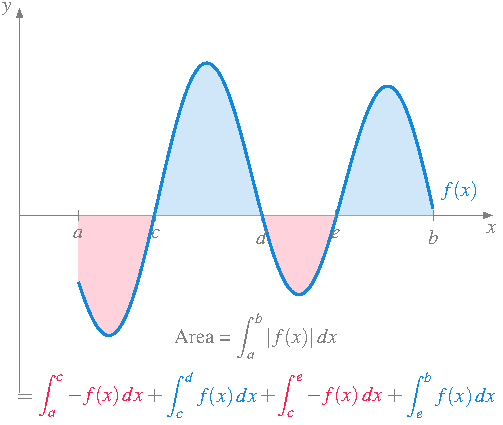
\includegraphics{img/integrales/area-funcion-positiva-negativa-2.pdf}

}

\caption{Area encerrada por una función positiva y negativa.}

\end{figure}

\begin{example}[]\protect\hypertarget{exm-area-funcion-positiva-negativa}{}\label{exm-area-funcion-positiva-negativa}

Veamos cómo calcular el area encerrada entre la gráfica de la función
\(f(x)=x^2-4x+3\) y el eje \(x\) en el intervalo \([0,4]\).

Si resolvemos la ecuación \(f(x)=0\) obtenemos dos raíces \(x=1\) y
\(x=3\), de manera que la función es positiva en el intervalo \((0,1)\)
y \((3,4)\) y negativa en el intervalo \((1,3)\). Por tanto, el área
encerrada entre la gráfica de la función y el eje \(x\) es

\begin{align*}
\int_0^4 |f(x)|\,dx 
&= \int_0^1 x^2-4x+3\,dx -\int_1^3 x^2-4x+3\,dx + \int_3^4 x^2+4x+3\,dx\\
&= \left[\frac{x^3}{3}-2x^2+3x\right]_0^1 + \left[\frac{x^3}{3}-2x^2+3x\right]_1^3 + \left[\frac{x^3}{3}-2x^2+3x\right]_3^4 \\
&= \frac{4}{3} - \frac{-4}{3} + \frac{4}{3} = 4
\end{align*}

\begin{figure}

{\centering 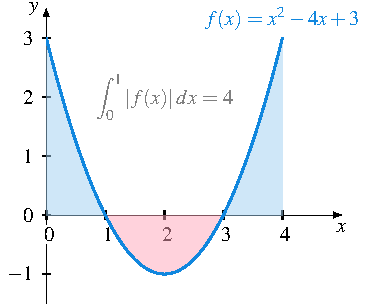
\includegraphics{img/integrales/area-parabola.pdf}

}

\caption{Area encerrada por la parábola \(f(x)=x^2-4x+3\).}

\end{figure}

\end{example}

\hypertarget{area-encerrada-entre-dos-funciones}{%
\subsection{Area encerrada entre dos
funciones}\label{area-encerrada-entre-dos-funciones}}

Si en lugar de calcular el área encerrada entre la gráfica de una
función \(f\) y el eje \(x\) en un intervalo \(I=[a,b]\), se quiere
calcular el area encerrada entre dos funciones \(f\) y \(g\) en un
intervalo \(I=[a,b]\), basta con integrar la diferencia entre las dos
funciones \(f-g\). Pero como \(f\) puede ser mayor que \(g\) en algún
subintervalo de \(I\) y menor en otros, para asegurarnos de calcular el
area correcta, hay que integrar el valor absoluto de la diferencia, es
decir,

\[
\int_a^b |f(x)-g(x)|\, dx
\]

Al igual que antes, para calcular esta integral mediante primitivas,
haciendo uso del teorema fundamental del cálculo, tendremos que
descomponer el intervalo de integración en subintervalos donde la
diferencia \(f-g\) sea sea positiva o negativa, integrar \(f-g\) en los
intervalos donde la diferencia es positiva, integrar \(-(f-g)=g-f\) en
los intervalos donde la diferencia es negativa, y finalmente, sumar las
areas correspondientes a cada subintervalo.

\begin{figure}

{\centering 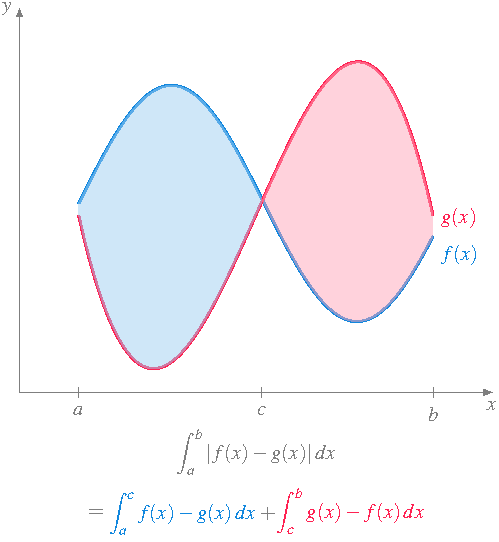
\includegraphics{img/integrales/area-entre-funciones.pdf}

}

\caption{Area encerrada entre dos funciones.}

\end{figure}

\begin{example}[]\protect\hypertarget{exm-area-funcion-positiva-negativa}{}\label{exm-area-funcion-positiva-negativa}

Veamos cómo calcular el area encerrada entre las gráficas de las
funciones \(f(x)=\operatorname{sen}(x)\) y \(g(x)=\cos(x)\) en el
intervalo \([0,\pi]\).

Si resolvemos la ecuación \(f(x)-g(x)=0\) obtenemos una raíz en
\(x=\pi/4\) en el intervalo de integración. Se cumple que \(f(x)<g(x)\)
\(\forall x\in\left(0,\frac{\pi}{4}\right)\) y \(f(x)>g(x)\)
\(\forall x\in\left(\frac{\pi}{4},\pi\right)\). Por tanto, el área
comprendida entre las gráficas de \(f\) y \(g\) en el intervalo
\([0,\pi]\) es

\begin{align*}
\int_0^\pi |f(x)-g(x)|\,dx 
&= \int_0^{\pi/4} \cos(x)-\operatorname{sen}(x)\,dx +\int_{\pi/4}^{\pi} \operatorname{sen}(x)-\cos(x)\,dx\\
&= \left[\operatorname{sen}(x)+\cos(x)\right]_0^{\pi/4} + \left[-\cos(x)-\operatorname{sen}(x)\right]_{\pi/4}^{\pi} \\
&= \sqrt{2}-1 +\sqrt{2}+1 = 2\sqrt{2}
\end{align*}

\begin{figure}

{\centering 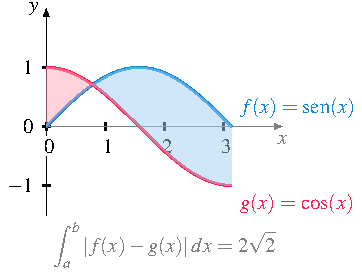
\includegraphics{img/integrales/area-entre-seno-coseno.pdf}

}

\caption{Area encerrada entre el seno y el coseno.}

\end{figure}

\end{example}

\hypertarget{sec-integrales-coordenadas-polares}{%
\subsection{Cálculo del area encerrada por una curva en coordenadas
polares}\label{sec-integrales-coordenadas-polares}}

En ocasiones, para calcular el area encerrada por una curva,
especialmente para curvas dadas mediante una ecuación implícita, resulta
más sencillo trabajar en coordenadas polares.

\begin{figure}

{\centering 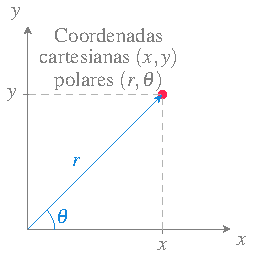
\includegraphics{img/integrales/coordenadas-polares.pdf}

}

\caption{Coordenadas polares.}

\end{figure}

Para pasar de coordenadas cartesianas a coordenadas polares, primero se
obtiene el valor de \(r\) aplicando el teorema de Pitágoras

\[
r = \sqrt{x^2+y^2}
\]

y después se obtiene el ángulo aplicando relaciones trigonométricas

\[
\theta =
\begin{cases}
\operatorname{arccos}\left(\frac{x}{r}\right) & \mbox{si $y\geq 0$}\\
-\operatorname{arccos}\left(\frac{x}{r}\right) & \mbox{si $y<0$}
\end{cases}
\]

suponiendo \(r\neq 0\).

Y para pasar de coordenadas polares a coordenadas cartesianas se aplican
las siguientes relaciones trigonométricas

\begin{align*}
x &= r \cos(\theta)\\
y &= r \operatorname{sen}(\theta)
\end{align*}

Para calcular el area encerrada por una curva dada en coordenadas
polares \(r=f(\theta)\) y las rectas \(\theta=a\) y \(\theta=b\), se
puede utilizar una aproximación similar a las sumas de Riemann,
descomponiendo el area en sectores de círculo con ángulos en una
partición \(P=\{\theta_0=a, \theta_1, \ldots, \theta_n=b\}\) de
\(I=[a,b]\). Si para cada uno de estos sectores se toma como radio el
ínfimo de \(f(\theta)\) en el correspondiente subintervalo, surgen las
sumas inferiores

\[
s(f,P) = \sum_{i=1}^n \pi m_i^2\frac{(\theta_i-\theta_{i-1})}{2\pi} = \sum_{i=1}^n \frac{m_i^2}{2}(\theta_i-\theta_{i-1}) 
\]

donde \(m_i=\inf\{f(\theta): \theta\in[\theta_{i-1},\theta_i]\}\) para
\(i=1,\ldots,n\).

Mientras que si para cada uno de estos sectores se toma como radio el
supremo de \(f(\theta)\) en el correspondiente subintervalo, surgen las
sumas superiores

\[
S(f,P) = \sum_{i=1}^n \pi M_i^2\frac{(\theta_i-\theta_{i-1})}{2\pi} = \sum_{i=1}^n \frac{M_i^2}{2}(\theta_i-\theta_{i-1}) 
\]

donde \(M_i=\sup\{f(\theta): \theta\in[\theta_{i-1},\theta_i]\}\) para
\(i=1,\ldots,n\).

\begin{figure}

{\centering 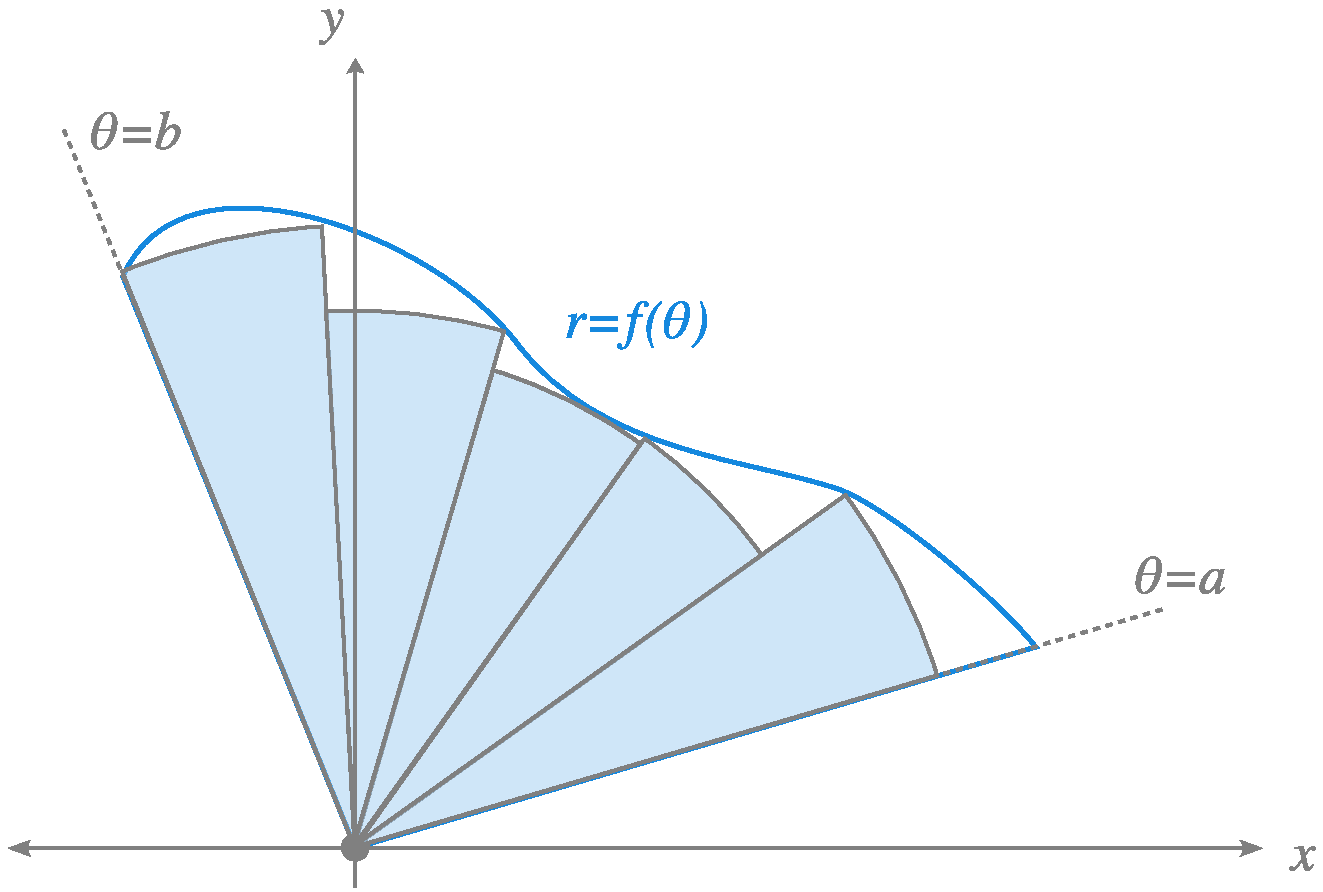
\includegraphics{img/integrales/sumas-riemann-polares.pdf}

}

\caption{Descomposición en sectores de círculos del area encerrada por
una curva en polares.}

\end{figure}

De forma análoga se puede definir \emph{integral inferior} de \(f\) en
\(I\) como
\(\underline{\int_a^b} f =\sup\{s(f,P): P\in \mathcal{P}(I)\}\) y la
\emph{integral superior} de \(f\) en \(I\) como el número
\(\overline{\int_a^b} f =\inf\{S(f,P): P\in \mathcal{P}(I)\}\), de
manera que, si la integral inferior coincide con la superior, la función
es integrable y

\[
\int_a^b \frac{f(\theta)^2}{2}\,d\theta
\]

mide el área encerrada por la curva \(r=f(\theta)\) y las rectas
\(\theta=a\) y \(\theta=b\).

\begin{figure}

{\centering 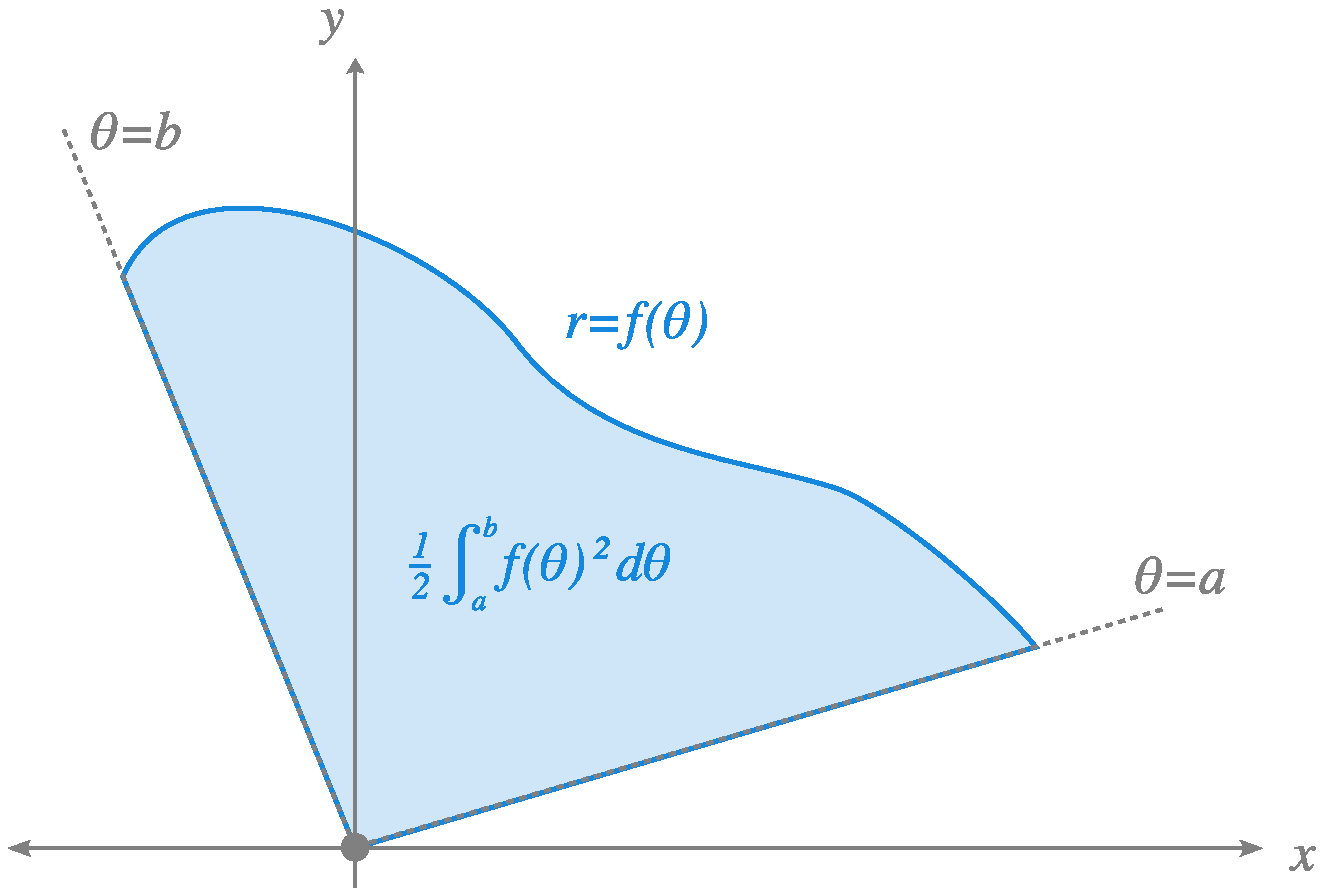
\includegraphics{img/integrales/integral-riemann-polares.pdf}

}

\caption{Area encerrada por una curva en coordenadas polares.}

\end{figure}

\begin{example}[]\protect\hypertarget{exm-area-semicírculo-polares}{}\label{exm-area-semicírculo-polares}

Un semicírculo de radio \(r\) puede expresarse en coordenadas polares
mediante la función \(f(\theta)=r\) para \(0\leq \theta\leq \pi\). Por
tanto, el área encerrada por este semicírculo es

\[
\int_0^{\pi} \frac{r^2}{2} \,d\theta = \left[\frac{r^2}{2}\theta\right]_0^\pi = \frac{r^2}{2}\pi.
\]

\end{example}

\begin{example}[]\protect\hypertarget{exm-area-curva-polar}{}\label{exm-area-curva-polar}

Veamos ahora cómo calcular el area encerrada por la curva polar
\(r=3\operatorname{sen}(2\theta)\).

\begin{align*}
\int_0^{2\pi} \frac{r^2}{2} 
&= \frac{1}{2}\int_0^{2\pi} (3\operatorname{sen}(2\theta))^2\,d\theta
= \frac{9}{2}\int_0^{2\pi} \operatorname{sen}(2\theta)^2\,d\theta \\
&= \frac{9}{2}\int_0^{2\pi} \frac{1 - \cos(2\theta)}{2}\,d\theta 
= \frac{9}{4}\left[\theta - \frac{\operatorname{sen}(2\theta)}{2}\right]_0^{2\pi} \\
&= \frac{9}{4}\left(2\pi - \frac{\operatorname{sen}(4\pi)}{2}\right)
= \frac{9}{4}2\pi 
= \frac{9}{2}\pi.
\end{align*}

\begin{figure}

{\centering 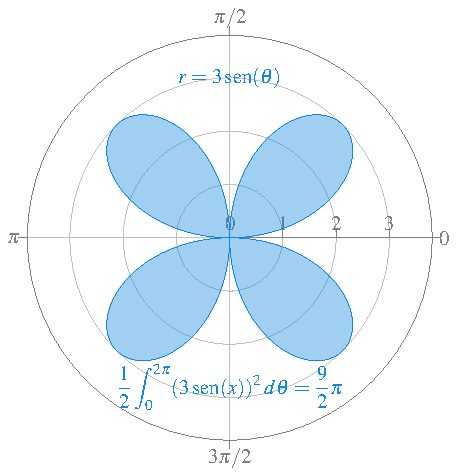
\includegraphics{img/integrales/area-curva-polar.pdf}

}

\caption{Area encerrada por la curva polar
\(r=3\operatorname{sen}(2\theta)\).}

\end{figure}

\end{example}

\hypertarget{cuxe1lculo-del-area-encerrada-por-dos-curvas-en-coordenadas-polares}{%
\subsection{Cálculo del area encerrada por dos curvas en coordenadas
polares}\label{cuxe1lculo-del-area-encerrada-por-dos-curvas-en-coordenadas-polares}}

También es posible calcular el area encerrada por dos curvas en
coordenadas polares de forma análoga a como se hizo para el area
encerrada entre dos funciones en coordenadas cartesianas.

Si tenemos dos curvas polares \(r=f(\theta)\) y \(r=g(\theta)\), con
\(f(\theta)\leq g(\theta)\) \(\forall \theta\in[a,b]\), el area
encerrada entre estas dos curvas en el intervalo \([a,b]\) puede
calcularse restando el area encerrada por \(g\) al area encerrada por
\(f\), es decir,

\[
\frac{1}{2} \int_a^b f(\theta)^2\,d\theta - \frac{1}{2} \int_a^b g(\theta)^2\,d\theta = \frac{1}{2} \int_a^b f(\theta)^2-g(\theta)^2\,d\theta
\]

\begin{figure}

{\centering 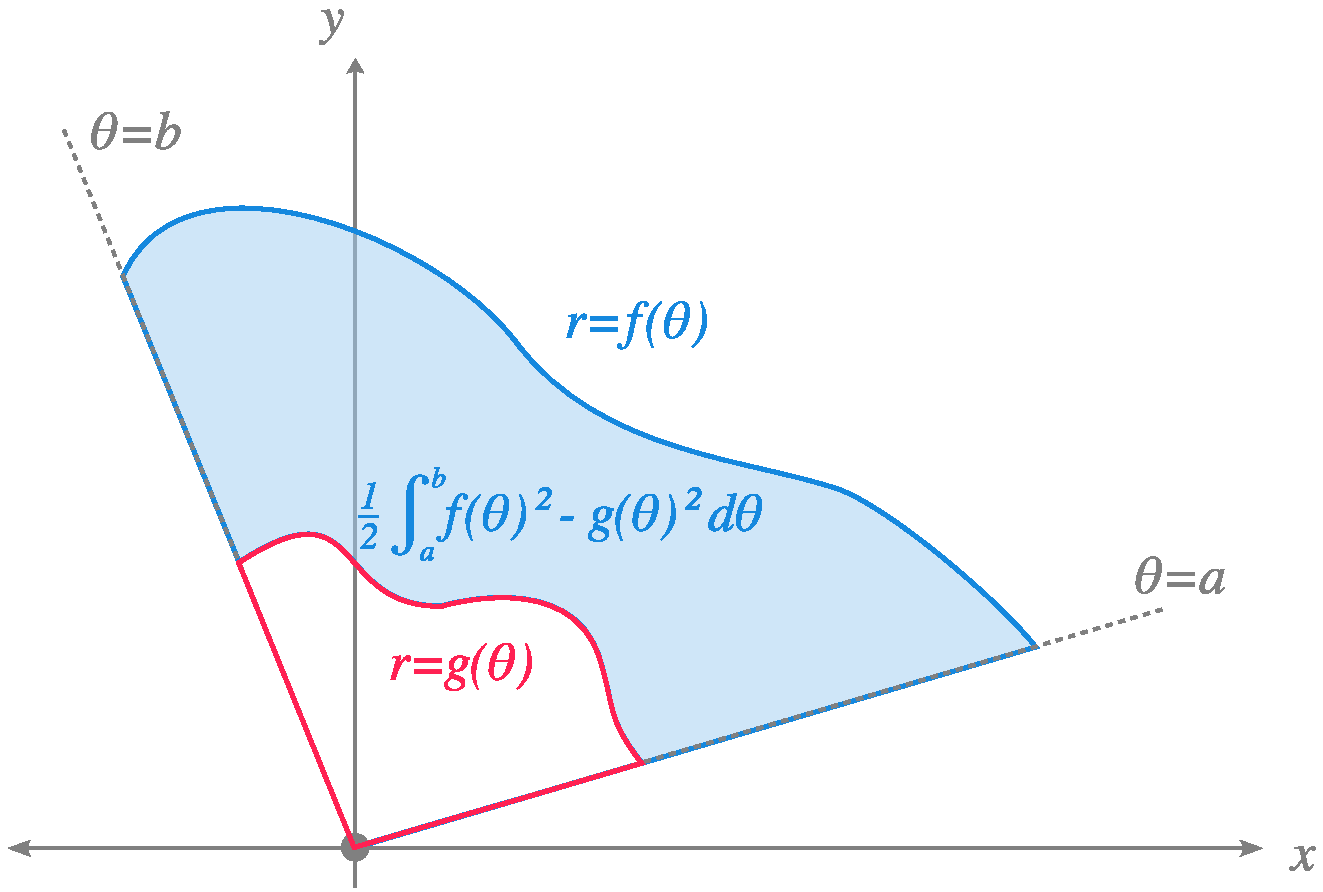
\includegraphics{img/integrales/area-entre-curvas-polares.pdf}

}

\caption{Area encerrada entre dos curvas polares\$.}

\end{figure}

En general, cuando \(f\) es mayor que \(g\) en algunos subintervalos de
\(I\) y menor en otros, habrá que descomponer el intervalo de
integración en subintervalos donde la diferencia \(f-g\) sea sea
positiva o negativa, integrar \(f-g\) en los intervalos donde la
diferencia es positiva, integrar \(-(f-g)=g-f\) en los intervalos donde
la diferencia es negativa, y finalmente, sumar las areas
correspondientes a cada subintervalo.

\begin{example}[]\protect\hypertarget{exm-area-entre-curvas-polares}{}\label{exm-area-entre-curvas-polares}

Vamos a calcular el area encerrada entre las curvas polares
\(r=3\cos(\theta)\) y \(r=1+\cos(\theta)\). Para ello primero debemos
determinar el intervalo de integración a partir de los puntos de corte
de las dos curvas.

\[
3\cos(\theta) = 1 + \cos(\theta) \Leftrightarrow \cos(\theta) = \frac{1}{2} \Leftrightarrow \theta = \operatorname{arccos}\left(\frac{1}{2}\right) = \pm \frac{\pi}{6}
\]

Así pues, el intervalo de integración es
\([-\frac{\pi}{6},\frac{\pi}{6}]\). Como en este intervalo
\(1+\cos(\theta) \leq 3\cos(\theta)\), el area encerrada entre estas dos
curvas es

\begin{align*}
\frac{1}{2}\int_{-\pi/6}^{\pi/6}f(\theta)^2-g(\theta)^2\,d\theta 
&= \frac{1}{2} \int_{-\pi/6}^{\pi/6}(3\cos(\theta))^2 - (1+\cos(\theta))^2 \,d\theta \\
&= \frac{1}{2} \int_{-\pi/6}^{\pi/6}(8\cos(\theta))^2 - 2\cos(\theta) - 1 \,d\theta \\
&= \frac{1}{2}\left(8\int_{-\pi/6}^{\pi/6}\cos(\theta)^2\,d\theta - 2\int_{-\pi/6}^{\pi/6}\cos(\theta)\,d\theta - \int_{-\pi/6}^{\pi/6}\,d\theta \right) \\
&= \frac{1}{2}\left([2\operatorname{sen}(2\theta)+4\theta]_{-\pi/6}^{\pi/6} - 2[\operatorname{sen}(\theta)]_{-\pi/6}^{\pi/6} - [\theta]_{-\pi/6}^{\pi/6} \right) \\
&= \frac{1}{2}\left(\sqrt{3}+\frac{4\pi}{6} +\sqrt{3} +\frac{4\pi}{6}\right)\\
&= \frac{\pi}{2}+\sqrt{3}-1 \approx 2.3028
\end{align*}

\begin{figure}

{\centering 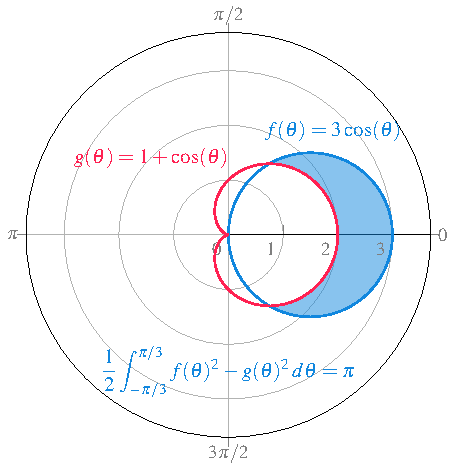
\includegraphics{img/integrales/area-entre-curvas-polares-2.pdf}

}

\caption{Area encerrada entre las curvas polares \(r=3\cos(\theta)\) y
\(r=1+\cos(\theta)\).}

\end{figure}

\end{example}

\hypertarget{integrales-impropias}{%
\section{Integrales impropias}\label{integrales-impropias}}

El concepto de integral definida de una función en un intervalo cerrado
\([a,b\){]} y se puede generalizar a intervalos no acotados y también a
funciones con discontinuidades de salto infinito.

\begin{definition}[Integral impropia de primer
tipo]\protect\hypertarget{def-integral-impropia-1}{}\label{def-integral-impropia-1}

Dada una función \(f:I\to\mathbb{R}\) integrable en \(I=[a,t]\) para
\(\forall t>a\), se define la \emph{integral impropia} de \(f\) en el
intervalo \([a,\infty)\) como el límite

\[
\int_a^\infty f(x)\,dx = \lim_{t\to\infty} \int_a^t f(x)\,dx
\]

siempre que este límite exista, en cuyo caso se dice que la integral
impropia converge.

Del mismo modo, si \(f\) es integrable en \(I=[t,a]\) para
\(\forall t<a\), se define la \emph{integral impropia} de \(f\) en el
intervalo \((-\infty, a]\) como el límite

\[
\int_{-\infty}^a f(x)\,dx = \lim_{t\to\infty} \int_t^a f(x)\,dx.
\]

Finalmente, si \(\int_{-\infty}^a f(x)\,dx\) y
\(\int_a^\infty f(x)\,dx\) convergen, se define la \emph{integral
impropia} de \(f\) en el intervalo \((-\infty, \infty)\) como

\[
\int_{-\infty}^\infty f(x)\,dx = \int_{-\infty}^a f(x)\,dx + \int_a^\infty f(x)\,dx
\]

\end{definition}

Para funciones positivas en los dominios de integración, estas
integrales impropias pueden interpretarse también como áreas. En
particular, \(\int_a^\infty f(x)\,dx\) es el area encerrada por la
gráfica de \(f\) y el eje \(x\) en el intervalo \([a,\infty)\),
\(\int_{-\infty}^\infty f(x)\,dx\) es el area encerrada por la gráfica
de \(f\) y el eje \(x\) en el intervalo \((-\infty,a]\) y
\(\int_{-\infty}^\infty f(x)\,dx\) es el area encerrada por la gráfica
de \(f\) y el eje \(x\) en todo \(\mathbb{R}\).

\begin{example}[]\protect\hypertarget{exm-integrales-impropias-1}{}\label{exm-integrales-impropias-1}

La integral impropia de la función \(f(x)=\frac{1}{x^2}\) converge en el
intervalo \([1,\infty]\) ya que

\[
\int_1^\infty \frac{1}{x^2}\,dx = \lim_{t\to\infty} \int_1^t \frac{1}{x^2}\,dx = \lim_{t\to\infty}\left[\frac{-1}{x}\right]_1^t = \lim_{n\to\infty} 1-\frac{1}{t} = 1.
\]

Por tanto, el área que queda encerrada por la gráfica de \(f\) y el eje
\(x\) por encima de \(1\) es finita y vale \(1\).

Sin embargo, la integral impropia de la función \(g(x)=\frac{1}{x}\)
diverge en el intervalo \([1,\infty]\) ya que

\[
\int_1^\infty \frac{1}{x}\,dx = \lim_{t\to\infty} \int_1^t \frac{1}{x}\,dx = \lim_{t\to\infty}\left[\ln(x)\right]_1^t = \lim_{n\to\infty} \ln(t) = \infty.
\]

Y por tanto, el área que queda encerrada por la gráfica de \(g\) y el
eje \(x\) por encima de \(1\) es infinita.

\end{example}

En estos casos la región encerrada por la gráfica de la función y el eje
\(x\) se extiende de manera infinita a lo largo del eje \(x\). La misma
idea puede aplicarse para calcular areas de regiones encerradas por la
gráfica de \(f\) y el eje \(y\) cuando estas regiones se extienden de
manera infinita porque la función no está acotada en algún valor del
dominio de integración.

\begin{definition}[Integral impropia de segundo
tipo]\protect\hypertarget{def-integral-impropia-2}{}\label{def-integral-impropia-2}

Dada una función \(f:I\to\mathbb{R}\) continua en \(I=[a,b)\) y
discontinua en \(b\), se define la \emph{integral impropia} de \(f\) en
\(I\) como el límite

\[
\int_a^b f(x)\,dx = \lim_{t\to b^-} \int_a^t f(x)\,dx
\]

siempre que este límite exista, en cuyo caso se dice que la integral
impropia converge.

\end{definition}

\hypertarget{sec-calculo-volumenes-integral}{%
\section{Cálculo de volúmenes}\label{sec-calculo-volumenes-integral}}

Otra de las aplicaciones habituales de las integrales es el cálculo de
volúmenes de cuerpos sólidos tridimensionales con secciones
transversales regulares. El procedimiento es similar al utilizado para
el cálculo de areas de regiones planas, pero en lugar de aproximar el
area mediante sumas de Riemann de rectángulos, se utilizan sumas de
Riemann de figuras geométricas de volumen conocido, habitualmente discos
o envoltorios cilíndricos. Para ello tomaremos secciones transversales
del cuerpo sólido del que se quiere calcular el volumen con respecto a
alguno de los ejes a lo largo de una partición del intervalo donde está
definido el sólido en ese eje.

\begin{figure}

{\centering 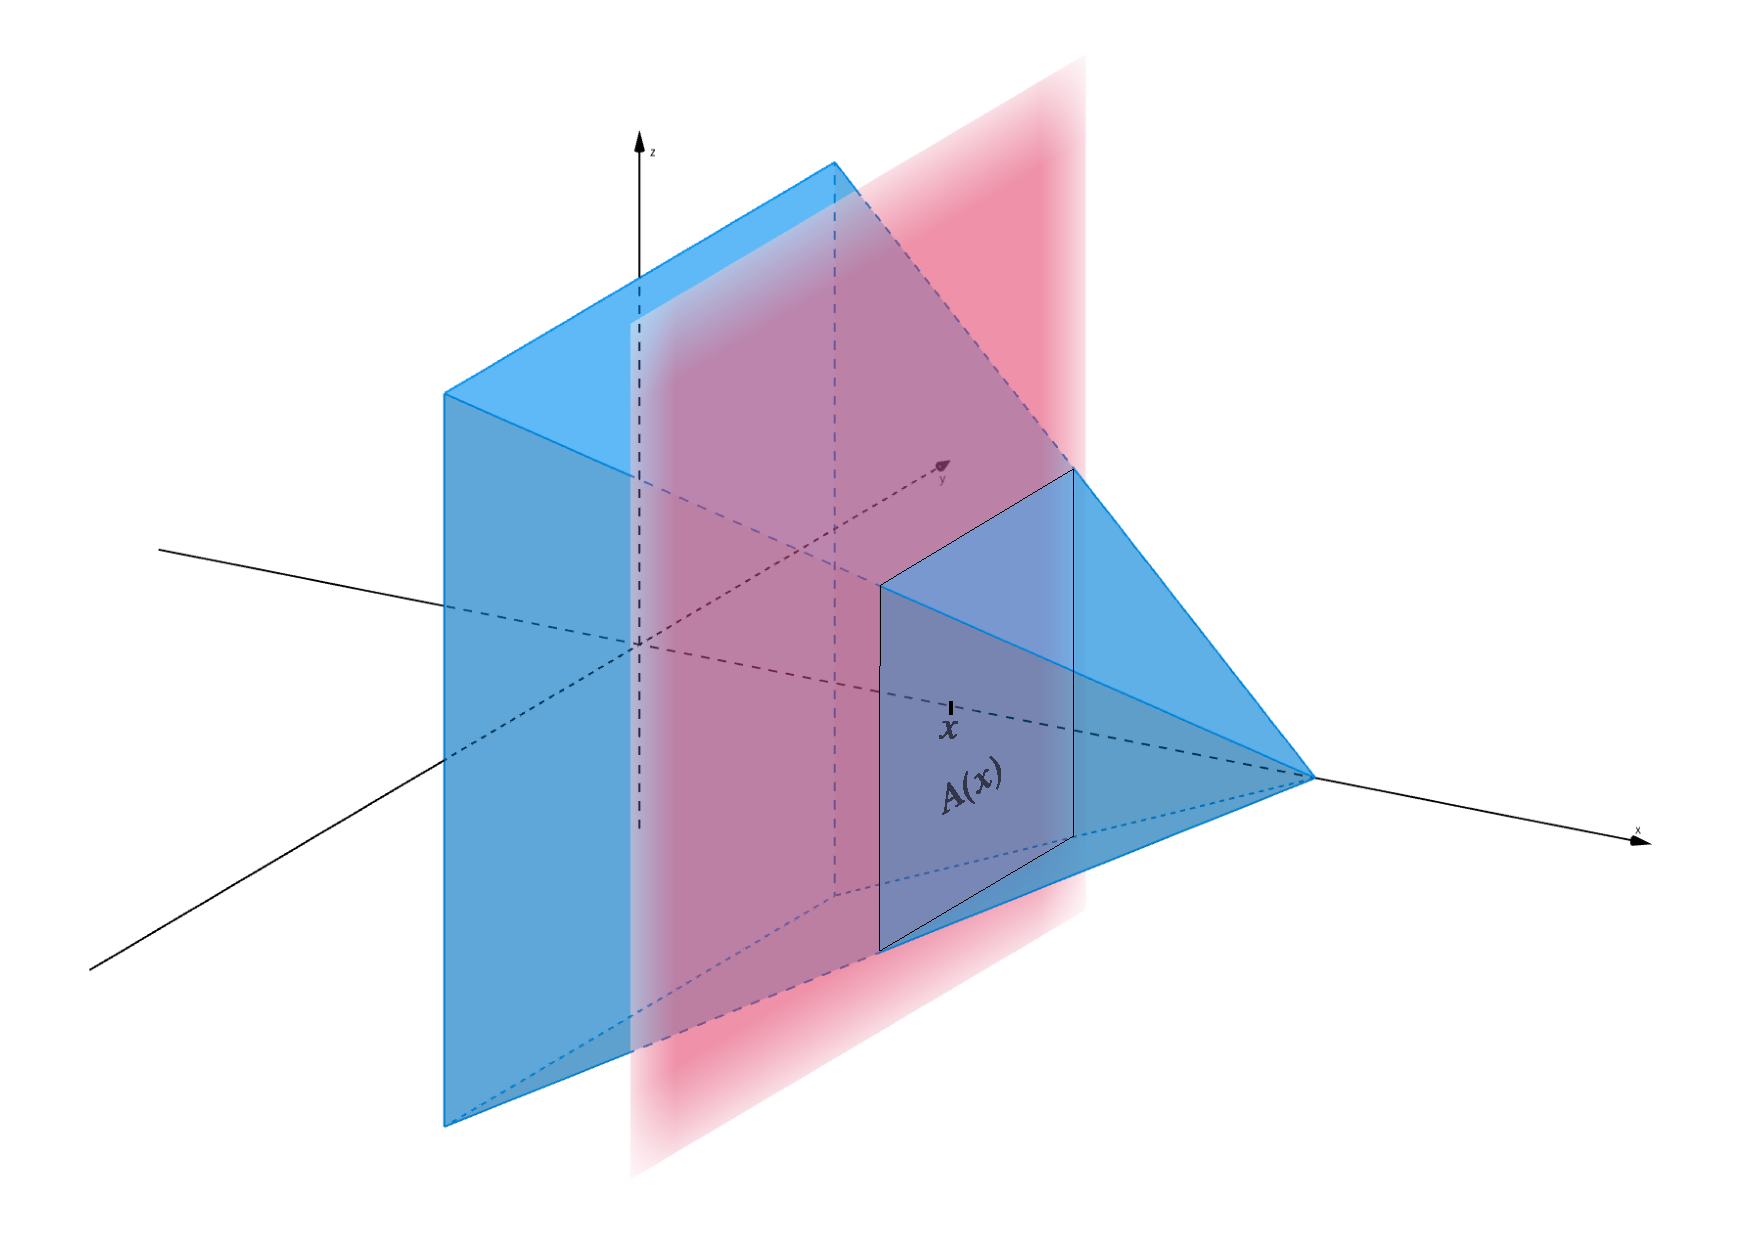
\includegraphics{img/integrales/seccion-transversal-piramide.pdf}

}

\caption{Sección transversal de un cuerpo sólido con respecto al eje
\(x\)}

\end{figure}

En general, si disponemos de una función \(A(x)\) que nos da el área de
la sección transversal del sólido para cada \(x\in[a,b]\), podemos tomar
una partición \(P_n=\{x_0=a,x_1,\ldots, x_n=b\}\) del intervalo
\([a,b]\) y aproximar el volumen del sólido en este intervalo mediante
las sumas inferior y superior de Riemann

\begin{align*}
s(A,P_n) &= \sum_{i=1}^n m_i(x_i-x_{i-1}),\quad m_i=\inf\{A(x): x\in(x_{i-1},x_i)\}\\
S(A,P_n) &= \sum_{i=1}^n M_i(x_i-x_{i-1}),\quad M_i=\sup\{A(x): x\in(x_{i-1},x_i)\}
\end{align*}

donde \(m_i (x_i-x_{i-1})\) es el volumen de un disco cilíndrico de base
\(m_i\) y altura \(x_i-x_{i-1}\), y \(M_i (x_i-x_{i-1})\) es el volumen
de un cilindro de base \(M_i\) y altura \(x_i-x_{i-1}\).

Como ya hemos visto, si
\(\lim_{n\to\infty} s(A,P_n) = \lim_{n\to\infty} S(A,P_n)\), la función
\(A(x)\) es integrable Riemann en el intervalo \([a,b]\) y

\[
\int_a^b A(x)\,dx = \lim_{n\to\infty} s(A,P_n) = \lim_{n\to\infty} S(A,P_n),
\]

mide el volumen del cuerpo sólido con secciones transversales de área
\(A(x)\) en el intervalo \([a,b]\).

\begin{example}[]\protect\hypertarget{exm-volumen-esfera}{}\label{exm-volumen-esfera}

Veamos cómo calcular el volumen de una esfera de radio \(r\) centrada en
el origen con ecuación \(x^2+y^2+z^2=r^2\). Si cortamos la esfera con
planos \(x=x_i\) perpendiculares al eje \(x\), sustituyendo en la
ecuación de la esfera, se tiene \(y^2+z^2=r^2-x_i^2\), por lo que se
obtienen secciones transversales circulares con radio
\(\sqrt{r^2-x_i^2}\), y, por tanto, el área de estas secciones
circulares será
\(\pi \left(\sqrt{r^2-x_i^2}\right)^2= \pi (r^2-x_i^2)\). Así pues, la
función que nos da el área de la sección transversal para cualquier
\(x\in[-r,r]\) es \(A(x)=\pi(r^2-x^2)\), y por tanto, podemos calcular
el volumen de la esfera con la integral definida

\begin{align*}
\int_{-r}^r \pi(r^2-x^2)\,dx 
&= \pi\left[r^2x-\frac{x^3}{3}\right]_{-r}^r \\
&= \pi\left(r^2r-\frac{r^3}{3}-\left(r^2(-r)-\frac{(-r)^3}{3}\right)\right) \\
&= 2r^3 - \frac{2r^3}{3} 
= \frac{4}{3}\pi r^3.
\end{align*}

\end{example}

\hypertarget{cuxe1lculo-de-voluxfamenes-de-suxf3lidos-de-revoluciuxf3n-con-discos-ciluxedndricos}{%
\subsection{Cálculo de volúmenes de sólidos de revolución con discos
cilíndricos}\label{cuxe1lculo-de-voluxfamenes-de-suxf3lidos-de-revoluciuxf3n-con-discos-ciluxedndricos}}

Cuando el sólido se obtiene rotando una función \(f(x)\) alrededor del
eje \(x\), se dice que el sólido resultante es un \emph{sólido de
revolución}.

\begin{figure}

{\centering 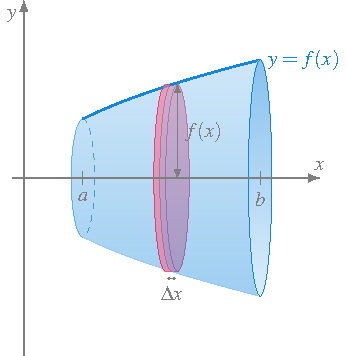
\includegraphics{img/integrales/disco-solido-revolucion.pdf}

}

\caption{Sólido de revolución.}

\end{figure}

Este tipo de sólidos tiene la particularidad de que todas sus secciones
transversales con respecto al eje de rotación son círculos de radio
\(f(x)\), por lo que el área de las secciones transversales es
\(A(x)=\pi f(x)^2\), y su volumen en el intervalo \([a,b]\) puede
calcularse mediante la integral definida

\[
\int_a^b \pi f(x)^2\,dx
\]

\begin{example}[]\protect\hypertarget{exm-volumen-cono-revolucion}{}\label{exm-volumen-cono-revolucion}

Si rotamos alrededor del eje \(x\) el segmento de la recta \(f(x)=2-x\)
correspondiente al intervalo \(x\in[0,2]\), se obtiene un cono con base
de radio \(2\) y altura \(2\). El volumen de este cono es

\begin{align*}
\int_0^2 \pi f(x)^2\,dx 
&= \int_0^2 \pi (2-x)^2\,dx 
= \pi \int_0^2 x^2-4x+4\,dx \\
&= \pi \left[\frac{x^3}{3}-2x^2+4x\right]_0^2
= \pi\left(\frac{2^3}{3}-2\cdot 2^2+4\cdot 2\right) 
= \frac{8}{3}\pi.
\end{align*}

\end{example}

\hypertarget{cuxe1lculo-de-voluxfamenes-de-suxf3lidos-de-revoluciuxf3n-con-envoltorios-ciluxedndricos}{%
\subsection{Cálculo de volúmenes de sólidos de revolución con
envoltorios
cilíndricos}\label{cuxe1lculo-de-voluxfamenes-de-suxf3lidos-de-revoluciuxf3n-con-envoltorios-ciluxedndricos}}

Otra forma de calcular volúmenes de sólidos de revolución es mediante
envoltorios o envolventes cilíndricas como los de figura de mas abajo.

\begin{figure}

{\centering 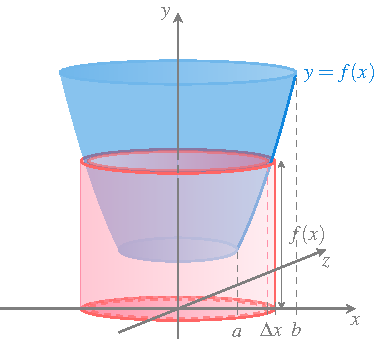
\includegraphics{img/integrales/envoltorio-cilindrico-solido-revolucion.pdf}

}

\caption{Envoltorio cilíndrico de un sólido de revolución.}

\end{figure}

Los envoltorios se construyen de forma que su base es un círculo de
radio \(x\in [a,b]\) y perpendicular al eje de rotación del sólido de
revolución y su altura es \(f(x)\), de manera que su área (sin contar el
área de las bases) es \(2\pi x f(x)\). Sumando las áreas de estos
infinitos envoltorios que se obtienen para cada \(x\in[a,b]\) se obtiene
al volumen del cuerpo sólido de revolución en el intervalo \([a,b]\)
mediante la integral definida

\[
\int_a^b 2\pi x f(x)\,dx
\]

\begin{example}[]\protect\hypertarget{exm-volumen-revolucion-envoltorios}{}\label{exm-volumen-revolucion-envoltorios}

El volumen del sólido de revolución que se obtiene al rotar alrededor
del eje \(y\) la función \(f(x)=x^2\) en el intervalo \([0,2]\) puede
calcularse usando tanto discos como envoltorios cilíndricos.

Si usamos discos discos cilíndricos debemos expresar \(x\) en función de
\(y\), es decir \(x=\sqrt{y}\) y calcular la siguiente integral definida
en el intervalo \([f(0),f(2)]\)

\[
\int_0^4 \pi g(y)^2\,dy 
= \int_0^4 \pi \left(\sqrt{y}\right)^2\,dy 
= \left[\pi\frac{y^2}{2}\right]_0^4 
= \pi\frac{4^2}{2} = 8\pi.
\]

Mientras que si usamos envoltorios cilíndricos hay que calcular la
integral

\[
\int_0^2 2\pi x f(x)\,dx
= \int_0^2 2\pi x\cdot  x^2\,dx 
= 2\pi\left[\frac{x^4}{4}\right]_0^2
= 2\pi \frac{2^4}{4} 
= 8\pi.
\]

\end{example}

\hypertarget{cuxe1lculo-de-la-longitud-de-una-curva}{%
\section{Cálculo de la longitud de una
curva}\label{cuxe1lculo-de-la-longitud-de-una-curva}}

Otra importante aplicación geométrica de las integrales es el cálculo de
la longitud de una curva dada por una función en un intervalo \([a,b]\).
Una vez más, la idea consiste en dividir el intervalo \([a,b]\) en \(n\)
subinvervalos de igual amplitud mediante una partición
\(P_n=\{x_0=a, x_1, \ldots, x_n=b\}\) con \(\Delta x = x_i-x{i-1}\)
\(i=1,\ldots,n\), y para cada subintervalo \([x_{i-1}, x_i]\) tomar el
segmento que une los puntos \((x_{i-1}, f(x_{i-1}))\) y
\((x_i,f(x_i))\). La suma de todos los segmentos correspondientes a la
partición tomada nos dará una aproximación de la longitud de la curva de
la función en el intervalo \([a,b]\).

\begin{figure}

{\centering 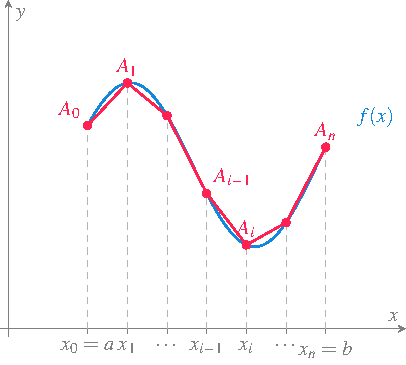
\includegraphics{img/integrales/aproximacion-longitud-curva.pdf}

}

\caption{Aproximación de la longitud de una curva mediante segmentos.}

\end{figure}

Aplicando el teorema de Pitágoras, es fácil ver que la longitud del
segmento correspondiente al subintervalo \([x_{i-1},x_i]\) es

\[
\sqrt{(x_i-x_{i-1})^2+(f(x_i)-f(x_{i-1}))^2} = \sqrt{\Delta x^2+(f(x_i)-f(x_{i-1}))^2}.
\]

Por otro lado, si \(f\) es diferenciable en \([x_{i-1},x_{i}]\), según
el teorema del valor medio, se tiene que existe un
\(x'_i\in [x_{i-1},x_i]\) tal que

\[
f'(x'_i) = \frac{f(x_i)-f(x_{i-1})}{x_i-x_{i-1}}
\]

de manera que

\[
f(x_i)-f(x_{i-1})=f'(x'_i)(x_i-x_{i-1}) = f'(x'_i)\Delta x,
\]

y la longitud del segmento puede expresarse como

\begin{align*}
\sqrt{\Delta x^2+(f(x_i)-f(x_{i-1}))^2}
&= \sqrt{\Delta x^2+(f'(x'_i)\Delta x^2}\\
&= \Delta x\sqrt{1+f'(x'_i)^2},
\end{align*}

y la suma de todos los segmentos resulta

\[
\sum_{i=1}^n \sqrt{1+f'(x'_i)^2}\Delta x
\]

Resulta evidente, que a medida que aumentemos el número de subintervalos
\(n\) de la partición, la aproximación de la longitud de la curva será
mejor y en el límite tendremos su valor exacto, que puede calcularse
mediante la integral definida

\[
\lim_{n\to\infty} \sum_{i=1}^n \sqrt{1+f'(x'_i)^2} \Delta x = \int_a^b \sqrt{1+f'(x)^2}\, dx,
\]

siempre y cuando \(f'(x)\) sea integrable en \([a,b]\).

\begin{example}[]\protect\hypertarget{exm-longitud-circunferencia}{}\label{exm-longitud-circunferencia}

Veamos cómo calcular la longitud de una circunferencia de radio \(1\)
centrada en el origen con ecuación \(x^2+y^2=1\). Resolviendo esta
ecuación para \(y\) se tiene que \(y=\pm \sqrt{1-x^2}\), y podemos tomar
la función \(f(x)=\sqrt{1-x^2}\) cuya gráfica es la semicircunferencia
superior.

La derivada de \(f\) es \(f'(x)=\frac{-x}{\sqrt{1-x^2}}\), de manera que
la longitud de la semicircunferencia es

\begin{align*}
\int_{-1}^1 \sqrt{1+\left(\frac{-x}{\sqrt{1-x^2}}\right)^2}\,dx 
&= \int_{-1}^1 \sqrt{1+\frac{x^2}{1-x^2}}\,dx 
= \int_{-1}^1 \sqrt{\frac{1}{1-x^2}}\,dx
\end{align*}

Esta integral es impropia ya que \(\frac{1}{1-x^2}\) tiende a \(\infty\)
cuando \(x\) tiende a \(\pm 1\), por lo que se tiene

\begin{align*}
\int_{-1}^1 \sqrt{\frac{1}{1-x^2}}\,dx
&= \lim_{t\to -1^+}\int_{t}^0 \sqrt{\frac{1}{1-x^2}}\,dx + \lim_{t\to 1^+}\int_0^t \sqrt{\frac{1}{1-x^2}}\,dx \\
&= -\lim_{t\to -1^+} \operatorname{arcsen}(t) + \lim_{t\to 1^+} \operatorname{arcsen}(t) 
= -\left(-\frac{\pi}{2}\right)+\frac{\pi}{2}
= \pi
\end{align*}

Y por tanto, la longitud de la circunferencia de radio \(1\) es el doble
\(2\pi\)

\end{example}

\hypertarget{cuxe1lculo-de-superficies-de-suxf3lidos-de-revoluciuxf3n}{%
\section{Cálculo de superficies de sólidos de
revolución}\label{cuxe1lculo-de-superficies-de-suxf3lidos-de-revoluciuxf3n}}

A partir del cálculo de la longitud de una curva plana, se puede
calcular la superficie del sólido de revolución que se obtiene al
girarla sobre el eje \(x\). Siguiendo con la idea de aproximar la
longitud de la curva mediante polígonos, al rotar alrededor del eje
\(x\) cada uno de los segmentos que forman parte del polígono, se
obtiene un tronco de cono.

Para calcular la superficie del envolvente del tronco de cono, veremos
primero cuál es el la superficie de este envolvente para un cono
completo. Si desplegamos el envolvente de un cono completo cortándolo
por su generatriz, se puede comprobar que se trata de un sector de
círculo con radio la generatriz del cono \(l\) y con arco de
circunferencia el perímetro del círculo de la base del cono \(2\pi r\).

\begin{figure}

\begin{minipage}[t]{0.50\linewidth}

{\centering 

\raisebox{-\height}{

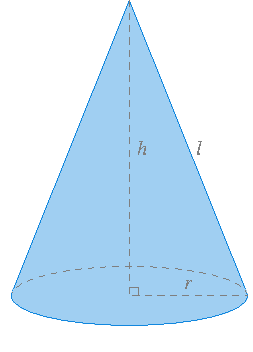
\includegraphics{./img/integrales/cono.pdf}

}

\caption{Cono con radio \(r\) y generatriz \(l\).}

}

\end{minipage}%
%
\begin{minipage}[t]{0.50\linewidth}

{\centering 

\raisebox{-\height}{

\includegraphics{./img/integrales/superficie-cono.pdf}

}

\caption{Superficie del envolvente del cono.}

}

\end{minipage}%

\end{figure}

El ángulo que describe este sector de círculo es
\(\theta = \frac{2\pi r}{l}\), y por tanto, su área es
\(\frac{\theta}{2}l^2= \frac{2\pi r}{2l}l^2 = \pi rl\).

Para calcular ahora la superficie del envolvente del tronco de cono como
del de la figura de más abajo, con radio menor \(r_1\) y radio mayor
\(r_2\), basta con restar a la superficie del cono de radio \(r_2\) y
generatriz \(l_2\), la superficie del cono de radio \(r_1\) y generatriz
\(l_1\).

\begin{figure}

{\centering \includegraphics{img/integrales/cono-truncado.pdf}

}

\caption{Tronco de cono con radio menor \(r_1\) y radio mayor \(r_2\).}

\end{figure}

La superficie del tronco de cono es, por tanto,

\[
\pi r_2 l_2 - \pi r_1 l_1 = \pi (r_2l_2-r_1l_1) = \pi(r_2(l+l_1)-r_1l_1) = \pi ((r_2-r_1)l_1+r_2l)
\]

Para poder expresar la superficie en función de \(l\), como por
semejanza de triángulos rectángulos se tiene que

\[
\frac{l_1}{r_1}=\frac{l_2}{r_2}=\frac{l+l_1}{r_2} \Leftrightarrow r_2l_1 = r_1(l+l_1) \Leftrightarrow r_1l = (r_2-r_1)l_1,
\]

de manera que sustituyendo en la expresión de la superficie del tronco
del cono, se tiene

\[
\pi ((r_2-r_1)l_1+r_2l) =  \pi (r_1l+r_2l) = \pi (r_1+r_2) l.
\]

Así pues, si tomamos una partición \(P_n=\{x_0=a, x_1, \ldots, x_n=b\}\)
del intervalo \([a,b]\), la superficie del tronco de cono
correspondiente al subintervalo \([x_{i-1},x_i]\) es

\[ 
S_i = \pi (f(x_{i-1}+f(x_i))l_i,
\]

donde \(l_i\) es la longitud del segmento que une los puntos
\((x_{i-1},f(x_{i-1}))\) y \((x_i,f(x_i))\), que como vimos en la
sección anterior, puede expresarse, gracias al teorema del valor medio,
como \(\sqrt{1+f'(x'_i)^2}\) para algún \(x'_i \in [x_{i-1},x_i]\). Por
tanto, la superficie del tronco de cono correspondiente al subintervalo
\([x_{i-1},x_i]\) puede expresarse finalmente como

\[
S_i = \pi (f(x_{i-1}+f(x_i))\sqrt{1+f'(x'_i)^2}
\] para algún \(x'_i\in [x_{i-1},x_i]\).

Si sumamos las superficies de todos los troncos de cono que se obtienen
para la partición \(P_n\),

\[
\sum_{i=1}^n S_i = \sum_{i=1}^n \pi (f(x_{i-1}+f(x_i))\sqrt{1+f'(x'_i)^2},
\]

se obtiene una aproximación de la superficie del sólido de revolución
generado al rotar la gráfica de la función \(f\) alrededor del eje
\(x\). A medida que aumentamos el número de intervalos en la partición,
la aproximación será mejor y en el límite cuanto \(n\) tiende a
\(\infty\), tendremos el valor exacto de la superficie de revolución.
Como ya se ha visto en las secciones anteriores, esta suma infinita es
la integral de rieman de las superficie del tronco de cono, es decir,

\[
S = \lim_{n\to\infty} \sum_{i=1}^n \pi (f(x_{i-1}+f(x_i))\sqrt{1+f'(x'_i)^2} = \int_a^b 2 \pi f(x)\sqrt{1+f'(x)^2}\,dx,
\]

ya que, cuando los intervalos se hacen infinitamente pequeños,
\(f(x_{i_1})\) y \(f(x_i)\) se aproximan cada vez más el uno al otro y,
en el límite, acaban siendo el mismo valor \(f(x)\), por lo que en la
integral se pone \(2 f(x)\).

\begin{example}[]\protect\hypertarget{exm-superficie-circunferencia}{}\label{exm-superficie-circunferencia}

Veamos cómo calcular la superficie de una esfera de radio \(r\) centrada
en el origen. Esta esfera es el sólido de revolución que surge al rotar
la función \(f(x)=\sqrt{r^2-x^2}\) alrededor del eje \(x\), por lo que
su superficie puede calcularse mediante la integral

\begin{align*}
\int_{-r}^r 2 \pi f(x)\sqrt{1+f'(x)^2}\,dx 
&= \int_{-r}^r 2 \pi \sqrt{r^2-x^2}\sqrt{1+\left(\frac{-x}{\sqrt{r^2-x^2}}\right)^2}\,dx \\
&= \int_{-r}^r 2 \pi \sqrt{r^2-x^2}\sqrt{1+\frac{x^2}{r^2-x^2}}\,dx \\
&= \int_{-r}^r 2 \pi \sqrt{r^2-x^2}\sqrt{\frac{r^2}{r^2-x^2}}\,dx \\
&= \int_{-r}^r 2 \pi \sqrt{r^2-x^2\frac{r^2}{r^2-x^2}}\,dx \\
&= \int_{-r}^r 2 \pi \sqrt{r^2}\,dx = \int_{-r}^r 2 \pi r\,dx \\
&= 2 \pi r [x]_{-r}^r  = 2\pi r(r-(-r)) = 4\pi r^2.
\end{align*}

\end{example}

\hypertarget{aplicaciones-fuxedsicas}{%
\section{Aplicaciones físicas}\label{aplicaciones-fuxedsicas}}

En esta sección presentamos varias aplicaciones de las integrales en
distintas áreas de la Física.

\hypertarget{cinemuxe1tica}{%
\subsection{Cinemática}\label{cinemuxe1tica}}

Como ya ese vió en la
\href{https://aprendeconalf.es/analisis-manual/07-derivadas.html\#interpretaci\%C3\%B3n-cinem\%C3\%A1tica-de-la-derivada}{interpretación
cinemática de la derivada}, cuando \(s(t)\) es una función que describe
la posición de un objeto que se mueve a lo largo del eje \(x\),
\(s'(t)\) es la velocidad instantánea del objeto en cada instante \(t\)
y \(s''(t)\) es la aceleración en cada instante \(t\).

Así pues, si conocemos la velocidad instantánea \(v(t)\) de un objeto en
cada instante \(t\), podemos averiguar su posición integrando la
velocidad. Como \$s(t) es una primitiva de \(v(t)\), según el teorema
fundamental del cálculo, se tiene

\[
\int_a^b v(t)\, dt = s(a)-s(b),
\]

es decir, la diferencia entre la posición el objeto en los instantes
\(t=b\) y \(t=a\).

\begin{tcolorbox}[enhanced jigsaw, colback=white, colbacktitle=quarto-callout-warning-color!10!white, title=\textcolor{quarto-callout-warning-color}{\faExclamationTriangle}\hspace{0.5em}{Advertencia}, rightrule=.15mm, coltitle=black, arc=.35mm, opacityback=0, colframe=quarto-callout-warning-color-frame, bottomtitle=1mm, titlerule=0mm, toptitle=1mm, bottomrule=.15mm, toprule=.15mm, breakable, opacitybacktitle=0.6, left=2mm, leftrule=.75mm]

La integral anterior mide el desplazamiento neto del objeto, que
coincide con el desplazamiento absoluto si la función velocidad es
positiva en el intervalo de integración, pero si toma valores positivos
y negativos, para calcular la distancia total recorrida por el objeto en
el intervalo \([a, b]\), es necesario integrar el valor absoluto de la
velocidad, tal y como se hizo para el cálculo de áreas en la
Sección~\ref{sec-calculo-area-funcion-ejex}.

\end{tcolorbox}

En general, suponiendo que el instante inicial en el que comienza el
movimiento es el instante \(t=0\), y por tanto, la posición inicial del
objeto es \(s(0)\), la posición que ocupa el objeto en cualquier
instante \(t\) viene dada por la integral

\[
s(t) = s(0) + \int_{0}^t v(x)\,dx.
\]

Del mismo modo, si conocemos la aceleración del objeto \(a(t)\) en cada
instante \(t\), podemos averiguar su velocidad integrando la
aceleración. Como \(v(t)\) es una primitiva de \(a(t)\), según el
teorema fundamental del cálculo, se tiene

\[
\int_a^b a(t)\, dt = v(t_1)-v(t_0),
\]

es decir, la diferencia entre la velocidades en los instantes \(a\) y
\(b\).

Si suponemos como antes, que el instante inicial en el que comienza el
movimiento es el instante \(t=0\), y por tanto, la velocidad inicial del
objeto es \(v(0)\), la velocidad del objeto en cualquier instante \(t\)
viene dada por la integral

\[
v(t) = v(0) + \int_{0}^t a(x)\,dx.
\]

Combinando estos dos resultados, es posible averiguar la posición que
ocupa el objeto si es conoce su aceleración.

\begin{example}[]\protect\hypertarget{exm-caida-libre}{}\label{exm-caida-libre}

Veamos cómo podemos deducir la famosa fórmula de la posición de un
objeto en caída libre. En este caso, supondremos que la posición inicial
del objeto es \(s(0)=s_0\) m y su velocidad inicial es \(v(0)=v_0\) m/s.
Además, supondremos que no hay rozamiento, por lo que la única fuerza
que actúa sobre el objeto es la gravedad, con una aceleración constante
\(g=9.8\) m/s\(^2\).

Integrando la aceleración obtenemos la velocidad del objeto en cada
instante \(t\).

\[
v(t) = v(0) + \int_{0}^t -g\,dx  = v_0 -g [x]_0^t = v_0-gt
\]

Ahora, integrando la velocidad obtenemos la posición el objeto en cada
instante \(t\).

\[
s(t) = s(0) + \int_{0}^t v_0-gx\,dx = s_0 + \left[v_0 x-g\frac{x^2}{2}\right]_0^t = s_0+v_0 t-g\frac{t^2}{2}.
\]

En el caso de que la posición inicial sea \(s_0=0\) m, y se parta de una
situación de reposo, es decir, \(v_0=0\) m/s, se llega a

\[
s(t) = -g\frac{t^2}{2}.
\]

\end{example}

\hypertarget{trabajo}{%
\subsection{Trabajo}\label{trabajo}}

Otra aplicación importante de las integrales en Física es el cálculo del
trabajo realizado al desplazar un objeto aplicándole una fuerza. En
mecánica clásica, si un objeto se desplaza en línea recta y su posición
viene dada por la función \(s(t)\), la \emph{fuerza} \(F\) ejercida
sobre el objeto viene dada por la
\href{https://es.wikipedia.org/wiki/Leyes_de_Newton\#Segunda_ley_de_Newton_o_ley_fundamental_de_la_din\%C3\%A1mica}{segunda
ley de Newton}

\[
F = m\cdot a
\]

donde \(m\) es la masa del objeto y \(a\) es la aceleración.

La unidad de medida de la fuerza en el Sistema Internacional (SI) es el
\emph{newton} N=kg\(\cdot\) m /s\(^2\), es decir, si se aplica \(1\) N a
un objeto de masa \(1\) kg, este sufrirá una aceleración de \(1\)
m/s\(^2\).

Cuando se aplica una fuerza sobre un objeto desplazándolo en línea recta
una determinada distancia, el \emph{trabajo} \(W\) realizado en ese
desplazamiento viene dado por el producto de la fuerza y la distancia
que recorre el objeto, es decir,

\[
W = F\cdot d
\]

Como la fuerza se mide en newtons, la unidad del trabajo en el SI es el
\emph{julio} \(J = N\cdot m\).

Cuando la fuerza es constante, el trabajo es proporcional a la distancia
recorrida.

\begin{example}[]\protect\hypertarget{exm-trabajo-gravedad}{}\label{exm-trabajo-gravedad}

Si levantamos una pesa de 1 kg desde el suelo hasta una altura de 2 m,
la fuerza ejercida es igual y opuesta a la que ejerce la gravedad, es
decir,

\[
F = m\cdot g = 1 \mbox{ kg} \cdot 9.81 \mbox{ m/s$^2$} = 9.8 \mbox{ N},
\]

y el trabajo realizado es

\[
W = F\cdot d = 9.81 \mbox{ N} \cdot 2 \mbox{ m} = 19.62 \mbox{ J}
\]

\end{example}

Cuando la fuerza que se aplica sobre el objeto no es constante, sino que
viene dada por una función \(f(x)\), el cálculo no es tan sencillo, pero
podemos aplicar la misma estrategia utilizada con las sumas de Riemann.
Si se quiere calcular el trabajo realizado al desplazar el objeto desde
la posición \(x=a\) hasta \(x=b\) aplicando una fuerza \(f(x)\), podemos
tomar una partición \(P_n=\{x_0=a, x_1, \ldots, x_n=b\}\) de \(n\)
intervalos de igual amplitud \(\Delta x\) y aproximar el trabajo
realizado en el intervalo \([x_{i-1},x_i]\) con
\(W_i= f(x'_i)(x_i-x_{i-1}) = f(x'_i)\Delta x\), donde \(x'_i\) es
cualquier valor del intervalo \([x_{i-1},x_i]\). De este modo, el
trabajo realizado en el intervalo \([a,b]\) puede aproximarse mediante
la suma

\[
W = \sum_{i=1}^n W_i = \sum_{i=1}^n f(x'_i)\Delta x.
\]

Como ya se ha visto, cuando el número de subintervalos tiende a
\(\infty\), en el límite, si la función \(f\) es integrable Riemann,
podemos obtener el trabajo exacto realizado con la integral

\[
\int_a^b f(x)\,dx
\]

\begin{tcolorbox}[enhanced jigsaw, colback=white, colbacktitle=quarto-callout-warning-color!10!white, title=\textcolor{quarto-callout-warning-color}{\faExclamationTriangle}\hspace{0.5em}{Advertencia}, rightrule=.15mm, coltitle=black, arc=.35mm, opacityback=0, colframe=quarto-callout-warning-color-frame, bottomtitle=1mm, titlerule=0mm, toptitle=1mm, bottomrule=.15mm, toprule=.15mm, breakable, opacitybacktitle=0.6, left=2mm, leftrule=.75mm]

La integral anterior mide el trabajo realizado al aplicar una fuerza en
el sentido del desplazamiento, es decir, cuando es positiva.

\end{tcolorbox}

\begin{example}[]\protect\hypertarget{exm-trabajo-fuerza-variable}{}\label{exm-trabajo-fuerza-variable}

La función \(f(x)=\frac{1}{1+x}\) determina la fuerza que actúa sobre
una partícula situada a una distancia \(x\) del origen de coordenadas.
El trabajo que se realiza al desplazar la partícula desde el origen al
punto \(1\) es

\[
W = \int_0^1 \frac{1}{1+x}\,dx = [\ln(1+x)]_0^1 = \ln(2) \mbox{ J}.
\]

\end{example}

\hypertarget{centro-de-masas}{%
\subsection{Centro de masas}\label{centro-de-masas}}

El centro de masas de un objeto o sistema de objetos es el punto
geométrico que dinámicamente se comporta como si en él estuvieran
aplicadas las fuerzas que actúan sobre el objeto. En el caso de un
sistema discreto, como por ejemplo una palanca sobre la que se coloca un
número finito de pesos, como en la figura de más abajo, determinar el
centro de gravedad es sencillo, ya que basta aplicar la
\href{https://es.wikipedia.org/wiki/Palanca}{ley de la palanca de
Arquímedes}, que establece

\[
m_1d_1 = m_2d_2
\]

\begin{figure}

{\centering \includegraphics{img/integrales/palanca.pdf}

}

\caption{Ley de la palanca.}

\end{figure}

Si colocamos las dos masas \(m_1\) y \(m_2\) sobre el eje \(x\) en las
posiciones \(x_1\) y \(x_2\) respectivamente, el centro de masas
\(\bar x\), que se correspondería con la posición donde habría que poner
el punto de apoyo de la palanca para que las dos masas la equilibraran,
se puede calcular aplicando la ley de la palanca,

\[
m_1(\bar x-x_1) = m_2(x_2-\bar x) \Leftrightarrow \bar x = \frac{m_1x_1+m_2x_2}{m_1+m_2},
\]

que, en realidad, es la media de las posiciones de \(x_1\) y \(x_2\)
ponderada de las masas.

Debido a la fuerza de la gravedad, cada objeto ejerce una fuerza sobre
la palanca que tiende a rotarla alrededor del punto de apoyo (si el
objeto está a la izquierda del punto de apoyo provocará una rotación en
sentido antihorario, mientras que si está a la derecha lo hará en
sentido horario). Esta efecto de rotación se conoce como \emph{momento}
o \emph{torque}, y para un objeto de masa \(m\) colocado en la posición
\(x\) de la palanca, toma el valor \(m\cdot x\cdot g\), y sus unidades
en el sistema internacional son \(N\cdot m\) (aunque ya hemos visto que
\(N\cdot m\) son julios, en este caso las unidades de los momentos no se
expresan en julios para distinguirlos del trabajo, ya que el trabajo es
una magnitud escalar, mientras que el momento es una magnitud
vectorial).

En general, si hay \(n\) objetos sobre la balanza, el centro de masas se
alcanzará en el punto \(\bar x\) que cumpla,

\[
\sum_{i=1}^n m_i(x_i-\bar x) = 0 \Leftrightarrow \bar x = \frac{\sum_{i=1}^n m_ix_i}{\sum_{i=1}^n m_i}.
\]

\hypertarget{centro-de-masas-de-una-varilla-con-densidad-variable}{%
\subsubsection{Centro de masas de una varilla con densidad
variable}\label{centro-de-masas-de-una-varilla-con-densidad-variable}}

Cuando el sistema contiene infinitos objetos de distintas masas, o se
trata de un objeto con una densidad variable, la cosa se complica. Por
ejemplo si queremos calcular el centro de masas de una varilla metálica
sobre un intervalo \([a,b]\), tal que su densidad viene dada por la
función \(f(x)\) kg/m, se puede descomponer el intervalo \([a,b]\) en
\(n\) subintervalos de igual amplitud mediante una partición
\(P_n=\{x_0=a, x_1, \ldots, x_n=b\)\}\$, con \(\Delta x=x_i-x_{i-1}\)
\(i=1, \ldots, n\). Podemos aproximar la masa de cada subintervalo,
asumiendo que tuviese una densidad constante \(f(x_i)\), como
\(m_i = f(x_i)(x_i-x_{i-1}) = f(x_i) \Delta x\), y por tanto,su momento
será \(x_im_i = x_i f(x_i)\Delta x\). De este modo, el centro de masas
de la varilla será aproximadamente, según la fórmula anterior,

\[
\bar x = \frac{\sum_{i=1}^n m_ix_i}{\sum_{i=1}^n m_i} = \frac{\sum_{i=1}^n x_if(x_i)\Delta x}{\sum_{i=1}^n f(x_i)\Delta x},
\]

que es el cociente de dos sumas de Riemann. De nuevo, si aumentamos el
número de subintervalos, cuando \(n\) tiende a \(\infty\), en el límite
se obtiene el valor exacto del centro de masas mediante el cociente de
dos integrales definidas

\[
\bar x = \frac{\int_a^b xf(x)\,dx}{\int_a^b f(x)\,dx}
\]

El centro de masas de una varilla situada sobre el intervalo \([5, 10]\)
con una densidad en cada punto \(x\) dada por la función \(f(x)=2x-1\)
es

\begin{align*}
\bar x 
&= \frac{\int_5^{10} xf(x)\,dx}{\int_5^{10} f(x)\,dx} 
= \frac{\int_5^{10} x(2x-1)\,dx}{\int_5^{10} 2x-1\,dx} \\
&= \frac{\left[2\frac{x^3}{3}-\frac{x^2}{2}\right]_5^{10}}{[x^2-x]_5^{10}}
= \frac{\left(2\frac{10^3}{3}-\frac{10^2}{2}-2\frac{5^3}{3}+\frac{5^2}{2}\right)}{10^2-10-5^2+5} \\
&= \frac{3275/6}{70} 
= 7.7976.
\end{align*}

\hypertarget{sec-centro-masas-region-plana-densidad-constante}{%
\subsubsection{Centro de masas de una región plana con densidad
fija}\label{sec-centro-masas-region-plana-densidad-constante}}

Cuando se tiene una región plana en \(\mathbb{R}^2\), su centro de masas
se conoce como \emph{centroide} y sus coordenadas se representan como
\((\bar x, \bar y)\). El cálculo de las coordenadas del centroide,
cuando todos los puntos de la región plana tienen la misma densidad
\(\delta\), se puede realizar de forma similar al cálculo del centro de
masas de una varilla con densidad variable.

Si la región está delimitada por una función \(f(x)\) y el eje \(x\) en
un intervalo \([a,b]\), al descomponer el intervalo \([a,b]\) en \(n\)
subintervalos de igual amplitud mediante una partición
\(P_n=\{x_0=a, x_1, \ldots, x_n=b\)\}\$, con \(\Delta x=x_i-x_{i-1}\)
\(i=1, \ldots, n\), se puede tomar como aproximación del área
correspondiente a cada subintervalo \([x_{i-1},x_i]\) el rectángulo con
base el intervalo y altura el valor de la función en el punto medio del
intervalo. Si llamamos al punto medio del subintervalo \(i\)-ésimo
subintervalo \(\bar x_i=\frac{x_{i-1}+x_i}{2}\), el área del rectángulo
correspondiente es \(A_i = f(\bar x_i)\Delta x\) y su masa
\(M_i = \delta f(\bar x_i)\Delta x\). Como todos los puntos tienen la
misma densidad \(\delta\), el centroide del rectángulo \(i\)-ésimo es
\((\bar x_i, \frac{1}{2}f(\bar x_i))\).

\begin{figure}

{\centering \includegraphics{img/integrales/suma-riemann-centro-masas.pdf}

}

\caption{Centroide de los rectángulos de una suma de Riemann.}

\end{figure}

El momento del rectángulo \(i\)-ésimo con respecto al eje \(y\) es

\[
\bar x_i M_i = x_i \delta f(\bar x_i)\Delta x 
\]

de manera que podemos aproximar el momento de la región con respecto al
eje \(y\) mediante la suma de Riemann

\[
\sum_{i=1}^n x_i \delta f(\bar x_i)\Delta x = \delta \sum_{i=1}^n x_i f(\bar x_i)\Delta x,
\]

y, tomando particiones cada vez con más subintervalos, en el límite
cuanto \(n\) tiende a \(\infty\) se obtiene el momento de la región con
respecto al eje \(y\) mediante la integral definida

\[
\delta \lim_{n\to \infty}\sum_{i=1}^n x_i f(\bar x_i)\Delta x = \delta \int_a^b x f(x)\, dx,
\]

por lo que se tiene

\[
\bar x = \frac{\delta \int_a^b x f(x)\, dx,}{\delta \int_a^b f(x)\, dx,} = \frac{\int_a^b x f(x)\, dx,}{\int_a^b f(x)\, dx,} 
\]

Del mismo modo, el momento del rectángulo \(i\)-ésimo con respecto al
eje \(x\) es

\[
\frac{1}{2}f(\bar x_i) M_i = \frac{1}{2}f(\bar x_i) \delta f(\bar x_i)\Delta x = \frac{1}{2}\delta f(\bar x_i)^2\Delta x
\]

de manera que podemos aproximar el momento de la región con respecto al
eje \(x\) mediante la suma de Riemann

\[
\sum_{i=1}^n \frac{1}{2}\delta f(\bar x_i)^2\Delta x = \frac{1}{2}\delta \sum_{i=1}^n f(\bar x_i)^2\Delta x,
\]

y, tomando particiones cada vez con más subintervalos, en el límite
cuanto \(n\) tiende a \(\infty\) se obtiene el momento de la región con
respecto al eje \(y\) mediante la integral definida

\[
\frac{1}{2}\delta \lim_{n\to \infty}\sum_{i=1}^n f(\bar x_i)^2\Delta x = \frac{1}{2}\delta \int_a^b f(x)^2\, dx,
\]

por lo que se tiene

\[
\bar y = \frac{\frac{1}{2}\delta \int_a^b f(x)^2\, dx,}{\delta \int_a^b f(x)\, dx,} = \frac{\int_a^b f(x)^2\, dx,}{2\int_a^b f(x)\, dx,}
\]

\begin{example}[]\protect\hypertarget{exm-centroide}{}\label{exm-centroide}

Veamos cómo calcular el centroide del semicírculo de ecuación
\(f(x)=\sqrt{1-x^2}\). En primer lugar calculamos el área del
semicírculo. Haciendo el cambio de variable
\(x=\operatorname{sen}(\theta)\), \(dx = \cos(\theta)d\theta\), se tiene

\begin{align*}
\int_{-1}^1 f(x)\,dx 
&= \int_{-1}^1 \sqrt{1-x^2}\,dx 
= \int_{-\pi/2}^{\pi/2} \sqrt{1-\operatorname{sen}(\theta)^2}\cos(\theta)\,d\theta \\
&= \int_{-\pi/2}^{\pi/2} \sqrt{\cos(\theta)^2}\cos(\theta)\,d\theta
= \int_{-\pi/2}^{\pi/2} \cos(\theta)^2\,d\theta \\
&= \int_{-\pi/2}^{\pi/2} \frac{1+\cos(\theta)}{2}\,d\theta
= \frac{1}{2}\left[\theta + \frac{1}{2}\operatorname{sen}(2\theta) \right]_{-\pi/2}^{\pi/2} \\
&= \frac{1}{2}\left(\frac{\pi}{2}+\frac{1}{2}\operatorname{sen}(\pi)+\frac{\pi}{2}-\frac{1}{2}\operatorname{sen}(-\pi)\right)\\
&= \frac{1}{2}\left(\frac{\pi}{2}+\frac{\pi}{2}\right)
= \frac{\pi}{2}.
\end{align*}

Y ahora calculamos el momento con respecto al eje \(x\).

\begin{align*}
\int_{-1}^1 xf(x)\,dx 
&= \int_{-1}^1 x\sqrt{1-x^2}\,dx 
= \int_{-\pi/2}^{\pi/2} \operatorname{sen}(\theta)\sqrt{1-\operatorname{sen}(\theta)^2}\cos(\theta)\,d\theta \\
&= \int_{-\pi/2}^{\pi/2} \operatorname{sen}(\theta)\sqrt{\cos(\theta)^2}\cos(\theta)\,d\theta
= \int_{-\pi/2}^{\pi/2} \operatorname{sen}(\theta)\cos(\theta)^2\,d\theta \\
&= \left[\frac{\cos(\theta)^3}{3} \right]_{-\pi/2}^{\pi/2} 
= \frac{1}{3}(\cos(\pi/2)^3-\cos(-\pi/2)^3)
= 0.
\end{align*}

De manera que

\[
\bar x = \frac{\int_{-1}^1 x f(x)\, dx,}{\int_{-1}^1 f(x)\, dx,} = \frac{0}{\pi/2} = 0
\]

Finalmente calculamos el momento con respecto al eje \(y\).

\begin{align*}
\frac{1}{2}\int_{-1}^1 f(x)^2\,dx 
&= \frac{1}{2}\int_{-1}^1 \sqrt{1-x^2}^2\,dx 
= \frac{1}{2}\int_{-1}^1 1-x^2\,dx
= \frac{1}{2}\left[x - \frac{x^3}{3}\right]_{-1}^1 \\
&= \frac{1}{2}\left(1-\frac{1^3}{3}-(-1)+\frac{(-1)^3}{3}\right)
= \frac{1}{2}\frac{4}{3}
= \frac{4}{6}. 
\end{align*}

y

\[
\bar y = \frac{1}{2}\frac{\int_{-1}^1 f(x)^2\, dx,}{\int_{-1}^1 f(x)\, dx,} = \frac{4/6}{\pi/2} = \frac{4}{3\pi}.
\]

Luego el centroide es \((0, \frac{4}{3\pi})\).

\end{example}

\hypertarget{aplicaciones-estaduxedsticas}{%
\section{Aplicaciones estadísticas}\label{aplicaciones-estaduxedsticas}}

Veremos a continuación otras aplicaciones de la integral más
relacionadas con la Estadística.

\hypertarget{sec-valor-medio-integral}{%
\subsection{Cálculo de la media de una
función}\label{sec-valor-medio-integral}}

Resulta sencillo calcular la media de un conjunto finito de números,
pero la cosa se complica cuando el conjunto de números es infinito, como
por ejemplo, cuando queremos calcular la temperatura media de un día.

En esta sección veremos cómo calcular el valor medio de una función
\(f\) en un intervalo \([a,b]\), siempre y cuando la función sea
integrable en el intervalo. La estrategia que seguiremos será la de
siempre. Tomaremos una partición \(P_n=\{x_0=a, x_1, \ldots, x_n=b\}\)
de \(n\) intervalos de igual amplitud \(\Delta x = \frac{b-a}{n}\) y
aproximar el valor medio de la función mediante la suma finita

\[
\sum_{i=1}^n \frac{f(x'_i)}{n} = \sum_{i=1}^n \frac{f(x'_i)}{\frac{b-a}{\Delta x}} = \frac{1}{b-a}\sum_{i=1}^n f(x'_i)\Delta x,
\]

donde \(x'_i\) es cualquier valor del intervalo \([x_{i-1},x_i]\).

Cuando el número de subintervalos tiende a \(\infty\), la suma anterior
se parecerá cada vez más al verdadero valor medio de la función en el
intervalo, y en el límite, si la función \(f\) es integrable Riemann, se
puede obtener el valor medio de la función mediante la integral definida

\[
\bar f[a,b] = \frac{1}{b-a}\int_a^b f(x)\,dx
\]

\begin{example}[]\protect\hypertarget{exm-valor-medio}{}\label{exm-valor-medio}

El valor medio de la función \(f(x)=\operatorname{sen}(x)\) en el
intervalo \([0,\pi/2]\) es

\begin{align*}
\bar f[0,\pi/2]
&= \frac{1}{\pi/2} \int_0^{\pi/2} f(x)\, dx 
= \frac{1}{\pi/2} \int_0^{\pi/2} \operatorname{sen}(x)\, dx \\
&= \frac{2}{\pi}[-\cos(x)]_0^{\pi/2}
= \frac{2}{\pi}(0+1)
= \frac{2}{\pi}
\end{align*}

Y el valor medio de esta misma función en el intervalo \([0,\pi]\) es

\begin{align*}
\bar f[0,\pi] 
&= \frac{1}{\pi} \int_0^{\pi} f(x)\, dx 
= \frac{1}{\pi} \int_0^{\pi} \operatorname{sen}(x)\, dx \\
&= \frac{2}{\pi}[-\cos(x)]_0^{\pi}
= \frac{2}{\pi}(-1+1)
= 0,
\end{align*}

por que la función seno es positiva en \([0,\pi/2]\) y negativa en
\([\pi/2, \pi]\), de manera que los valores positivos se compensan con
los negativos y se obtiene una media 0.

\end{example}

\bookmarksetup{startatroot}

\hypertarget{geometruxeda-vectorial-del-plano-y-del-espacio-reales}{%
\chapter{Geometría vectorial del plano y del espacio
reales}\label{geometruxeda-vectorial-del-plano-y-del-espacio-reales}}

Para proceder al estudio analítico de las funciones de varias variables
y de las funciones vectoriales se necesita introducir el concepto de
vector y algunas propiedades geométricas del plano euclídeo
\(\mathbb{R}^2\) y del espacio euclídeo \(\mathbb{R}^3\). Muchas de
estas propiedades se pueden generalizar fácilmente a espacios de
cualquier dimensión. En este capítulo introducimos estos los conceptos
básicos de geometría vectorial necesarios para los próximos capítulos.

\hypertarget{escalares-y-vectores}{%
\section{Escalares y vectores}\label{escalares-y-vectores}}

\hypertarget{escalares}{%
\subsection{Escalares}\label{escalares}}

Algunos fenómenos de la naturaleza pueden describirse mediante un número
referido a una unidad de medida.

\begin{definition}[Escalar]\protect\hypertarget{def-escalar}{}\label{def-escalar}

Un \emph{escalar} es un número que sirve para expresar una magnitud sin
dirección.

\end{definition}

\begin{example}[]\protect\hypertarget{exm-escalar}{}\label{exm-escalar}

La estatura o el peso de una persona, el volumen de un depósito, la
temperatura de un gas, el trabajo realizado por una fuerza sobre un
objeto, la carga eléctrica o el tiempo que tarda un móvil en recorrer
una distancia, son escalares.

\end{example}

Sin embargo, existen otros fenómenos que no pueden describirse
adecuadamente mediante un escalar. Si, por ejemplo, un navegante quiere
poner rumbo a puerto y sólo conoce de la intensidad del viento, no sabrá
qué dirección tomar. La descripción del viento requiere dos elementos,
su intensidad y su dirección.

\hypertarget{vectores}{%
\subsection{Vectores}\label{vectores}}

\begin{definition}[Vector]\protect\hypertarget{def-vector}{}\label{def-vector}

Un \emph{vector} es un objeto geométrico que tiene asociada una magnitud
o longitud y una dirección. El vector con longitud 0 se conoce como
\emph{vector nulo}, se representa \(\mathbf{O}\) y es el único vector
que no tiene dirección.

\end{definition}

\begin{example}[]\protect\hypertarget{exm-vector}{}\label{exm-vector}

La velocidad y la aceleración de un móvil o la fuerza que se aplica
sobre un objeto, son vectores.

\end{example}

Geométricamente, en un espacio euclídeo, un vector se representa
mediante un segmento orientado, es decir, una flecha.

\begin{figure}

{\centering \includegraphics{img/geometria-plano-espacio/vector.pdf}

}

\caption{Vector.}

\end{figure}

\hypertarget{representaciuxf3n-de-un-vector}{%
\subsection{Representación de un
vector}\label{representaciuxf3n-de-un-vector}}

Un segmento orientado puede ubicarse en diferentes lugares dentro de un
espacio euclídeo. Sin embargo, con independencia de donde esté situado,
si la longitud y la dirección no varían, dicho segmento representará
siempre el mismo vector.

Esto permite representar todos los vectores con un mismo origen, el
origen en sistema de coordenadas cartesianas. Así, en cualquier espacio
euclídeo, un vector queda determinado por las \emph{coordenadas} del
punto que determina su extremo final.

\begin{figure}

{\centering \includegraphics{img/geometria-plano-espacio/coordenadas-vector.pdf}

}

\caption{Coordenadas de un vector.}

\end{figure}

\hypertarget{vector-a-partir-de-dos-puntos}{%
\subsection{Vector a partir de dos
puntos}\label{vector-a-partir-de-dos-puntos}}

Dados dos puntos \(P\) y \(Q\) de un espacio euclídeo, el vector con
origen en \(P\) y final en \(Q\) tiene coordenadas \(\vec{PQ}=Q-P\).

\begin{example}[]\protect\hypertarget{exm-vector-dos-puntos}{}\label{exm-vector-dos-puntos}

Sean los puntos \(P=(1,1)\) y \(Q=(3,4)\) del plano real
\(\mathbb{R}^2\), entonces

\[\vec{PQ} = Q-P = (3,4)-(1,1) = (3-1,4-1) = (2,3).\]

\begin{figure}

{\centering \includegraphics{img/geometria-plano-espacio/vector-puntos.pdf}

}

\caption{Definción de un vector a partir de dos puntos.}

\end{figure}

\end{example}

\hypertarget{muxf3dulo-de-un-vector}{%
\subsection{Módulo de un vector}\label{muxf3dulo-de-un-vector}}

\begin{definition}[Módulo de un
vector]\protect\hypertarget{def-modulo-vector}{}\label{def-modulo-vector}

Dado un vector \(\mathbf{v}=(v_1,\cdots,v_n)\) en \(\mathbb{R}^n\), se
define el \emph{módulo} de \(\mathbf{v}\) como

\[
\lvert \mathbf{v} \rvert = \sqrt{v_1^2+ \cdots + v_n^2}.
\]

\end{definition}

\begin{proposition}[]\protect\hypertarget{prp-modulo-vector}{}\label{prp-modulo-vector}

El módulo de un vector coincide con la longitud del segmento que
representa el vector.

\end{proposition}

\begin{tcolorbox}[enhanced jigsaw, colback=white, colbacktitle=quarto-callout-note-color!10!white, title=\textcolor{quarto-callout-note-color}{\faInfo}\hspace{0.5em}{Demostración}, rightrule=.15mm, coltitle=black, arc=.35mm, opacityback=0, colframe=quarto-callout-note-color-frame, bottomtitle=1mm, titlerule=0mm, toptitle=1mm, bottomrule=.15mm, toprule=.15mm, breakable, opacitybacktitle=0.6, left=2mm, leftrule=.75mm]

\begin{proof}

Probaremos primero la proposición para el plano real \(\mathbb{R}^2\).
Supongamos que el vector tiene componentes \(\mathbf{v}=(v_1,v_2)\). En
este caso, tal y como se puede apreciar en la siguiente figura, el
vector es la hipotenusa del triángulo rectángulo con catetos de longitud
\(v_1\) y \(v2\).

\begin{figure}[H]

{\centering \includegraphics{img/geometria-plano-espacio/modulo-vector-plano.pdf}

}

\caption{Módulo de un vector en el plano.}

\end{figure}

Por tanto, aplicando el teorema de Pitágoras, se tiene que la longitud
de \(\mathbf{v}\) es

\[
\sqrt{(v_1^2+v_2^2} = |\mathbf{v}|.
\]

Veamos ahora que también es cierto en el espacio real \(\mathbb{R}^3\).
Supongamos que el vector tiene componentes \(\mathbf{v}=(v_1,v_2,v_3)\).
En este caso, tal y como se puede apreciar en la siguiente figura, el
vector es la hipotenusa del triángulo rectángulo con catetos de longitud
\(|\mathbf{w}|\) y \(v3\), donde \(\mathbf{w}\) es el vector que resulta
de proyectar \(\mathbf{v}\) sobre el plano \(xy\), es decir,
\(\mathbf{w}=(v_1,v_2)\).

\begin{figure}[H]

{\centering \includegraphics{img/geometria-plano-espacio/modulo-vector-espacio.png}

}

\caption{Módulo de un vector en el espacio.}

\end{figure}

Como hemos visto para el plano real, se cumple que
\(|\mathbf{w}| = \sqrt{v_1^2+v_2^2}\), y aplicando de nuevo el teorema
de Pitágoras, se tiene que la longitud de \(\mathbf{v}\) es

\[
\sqrt{|\mathbf{w}|^2+v_3^2} = \sqrt{v_1^2+v_2^2+v_3^2} = |\mathbf{v}|.
\]

El caso general para el espacio \(\mathbb{R}^n\) puede probarse
fácilmente por inducción y se deja como ejercicio.

\end{proof}

\end{tcolorbox}

\begin{example}[]\protect\hypertarget{exm-modulo-vector}{}\label{exm-modulo-vector}

Sea \(\mathbf{u}=(3,4)\) un vector en \(\mathbb{R}^2\), entonces

\[
\lvert \mathbf{u} \rvert = \sqrt{3^2+4^2} = \sqrt{25} = 5.
\]

Sea \(\lvert \mathbf{v}\rvert =(4,7,4)\) un vector en \(\mathbb{R}^3\),
entonces

\[
\lvert \mathbf{v} \vert = \sqrt{4^2+7^2+4^2} = \sqrt{81} = 9.
\]

\end{example}

\hypertarget{vectores-unitarios}{%
\subsection{Vectores unitarios}\label{vectores-unitarios}}

\begin{definition}[Vector
unitario]\protect\hypertarget{def-vector-unitario}{}\label{def-vector-unitario}

Se dice que un vector \(\mathbf{v}\) en \(\mathbb{R}^n\) es
\emph{unitario} si su módulo es 1, es decir
\(\lvert \mathbf{v}\rvert=1\).

\end{definition}

Especial atención merecen los vectores unitarios que siguen la dirección
de los ejes de coordenadas, estos vectores se llaman \emph{vectores
coordenados}.

En \(\mathbb{R}^2\) los vectores coordenados son

\[\mathbf{i}=(1,0)\mbox{ y }\mathbf{j}=(0,1)\]

\begin{figure}

{\centering \includegraphics{img/geometria-plano-espacio/vectores-coordenados-plano.pdf}

}

\caption{Vectores coordenados en el plano real.}

\end{figure}

En \(\mathbb{R}^3\) los vectores coordenados son

\[\mathbf{i}=(1,0,0)\mbox{, }\mathbf{j}=(0,1,0) \mbox{ y } \mathbf{k}=(0,0,1)\]

\begin{figure}

{\centering \includegraphics{img/geometria-plano-espacio/vectores-coordenados-espacio.pdf}

}

\caption{Vectores coordenados en el espacio real.}

\end{figure}

\hypertarget{suma-de-vectores}{%
\subsection{Suma de vectores}\label{suma-de-vectores}}

\begin{definition}[Suma de
vectores]\protect\hypertarget{def-suma-vectores}{}\label{def-suma-vectores}

Dados dos vectores \(\mathbf{u}=(u_1,\cdots,u_n)\) y
\(\mathbf{v}=(v_1,\cdots,v_n)\) en \(\mathbb{R}^n\), se define la
\emph{suma} de \(\mathbf{u}\) y \(\mathbf{v}\) como

\[
\mathbf{u}+\mathbf{v} = (u_1+v_1,\ldots, u_n+v_n).
\]

\end{definition}

\begin{figure}

{\centering \includegraphics{img/geometria-plano-espacio/suma-vectores.pdf}

}

\caption{Suma de vectores.}

\end{figure}

\begin{example}[]\protect\hypertarget{exm-suma-vectores}{}\label{exm-suma-vectores}

Sean \(\mathbf{u}=(3,1)\) y \(\mathbf{v}=(2,3)\) dos vectores en
\(\mathbb{R}^2\), entonces

\[
\mathbf{u}+\mathbf{v} = (3+2,1+3) = (5,4).
\]

\end{example}

\hypertarget{producto-de-un-vector-por-un-escalar}{%
\subsection{Producto de un vector por un
escalar}\label{producto-de-un-vector-por-un-escalar}}

\begin{definition}[Producto de un vector por un
escalar]\protect\hypertarget{def-producto-por-escalar}{}\label{def-producto-por-escalar}

Dado un vector \(\mathbf{v}=(v_1,\cdots,v_n)\) en \(\mathbb{R}^n\), y un
escalar \(a\in \mathbb{R}\), se define el \emph{producto} de \(a\) por
\(\mathbf{v}\) como

\[
a\mathbf{v} = (av_1,\ldots, av_n).
\]

\end{definition}

\begin{figure}

{\centering \includegraphics{img/geometria-plano-espacio/producto-vector-por-escalar.pdf}

}

\caption{Producto de un vector por un escalar.}

\end{figure}

\begin{example}[]\protect\hypertarget{exm-producto-por-escalar}{}\label{exm-producto-por-escalar}

Sean el vector \(\mathbf{v}=(2,1)\) en \(\mathbb{R}^2\) y el escalar
\(a=2\), entonces

\[
a\mathbf{v} = 2(2,1) = (4,2).
\]

\end{example}

\hypertarget{expresiuxf3n-de-un-vector-como-combinaciuxf3n-lineal-de-los-vectores-coordenados}{%
\subsection{Expresión de un vector como combinación lineal de los
vectores
coordenados}\label{expresiuxf3n-de-un-vector-como-combinaciuxf3n-lineal-de-los-vectores-coordenados}}

La suma de vectores y el producto de un vector por un escalar permite
expresar cualquier vector como una combinación lineal de los vectores
coordenados.

En el caso del espacio real \(\mathbb{R}^3\), cualquier vector
\(\mathbf{v}=(v_1,v_2,v_3)\) puede expresarse como

\[\mathbf{v}=(v_1,v_2,v_3) = v_1\mathbf{i}+v_2\mathbf{j}+v_3\mathbf{k}.\]

\begin{figure}

{\centering \includegraphics{img/geometria-plano-espacio/combinacion-lineal-vectores-coordenados.pdf}

}

\caption{Expresión de un vector como combinación lineal de los vectores
coordenados.}

\end{figure}

\hypertarget{producto-escalar}{%
\subsection{Producto escalar}\label{producto-escalar}}

Ya hemos visto como sumar y restar vectores, y cómo multiplicarlos por
un escalar, pero no hemos visto cómo multiplicar vectores. Existen
diferentes formas de multiplicar dos vectores, una de ellas es el
\emph{producto escalar} que tiene aplicaciones muy interesantes.

\begin{definition}[Producto
escalar]\protect\hypertarget{def-producto-escalar}{}\label{def-producto-escalar}

Dados dos vectores \(\mathbf{u}=(u_1,\cdots,u_n)\) y
\(\mathbf{v}=(v_1,\cdots,v_n)\) en \(\mathbb{R}^n\), se define el
\emph{producto escalar} de \(\mathbf{u}\) y \(\mathbf{v}\) como

\[
\mathbf{u}\cdot \mathbf{v} = u_1v_1 + \cdots + u_nv_n.
\]

\end{definition}

\begin{tcolorbox}[enhanced jigsaw, colback=white, colbacktitle=quarto-callout-warning-color!10!white, title=\textcolor{quarto-callout-warning-color}{\faExclamationTriangle}\hspace{0.5em}{Advertencia}, rightrule=.15mm, coltitle=black, arc=.35mm, opacityback=0, colframe=quarto-callout-warning-color-frame, bottomtitle=1mm, titlerule=0mm, toptitle=1mm, bottomrule=.15mm, toprule=.15mm, breakable, opacitybacktitle=0.6, left=2mm, leftrule=.75mm]

El resultado del producto escalar de dos vectores no es un vector, sino
un escalar.

\end{tcolorbox}

\begin{example}[]\protect\hypertarget{exm-producto-escalar}{}\label{exm-producto-escalar}

Sean \(\mathbf{u}=(3,1)\) y \(\mathbf{v}=(2,3)\) dos vectores en
\(\mathbb{R}^2\), entonces

\[
\mathbf{u}\cdot\mathbf{v} = 3\cdot 2 +1\cdot 3 = 9.
\]

\end{example}

\begin{proposition}[Propiedades del producto
escalar]\protect\hypertarget{prp-propiedades-producto-escalar}{}\label{prp-propiedades-producto-escalar}

Dados los vectores \(\mathbf{u}\), \(\mathbf{v}\) y \(\mathbf{w}\) en
\(\mathbb{R}^n\), se cumple que

\begin{enumerate}
\def\labelenumi{\alph{enumi}.}
\tightlist
\item
  \(\mathbf{v}\cdot\mathbf{v} = |\mathbf{v}|^2\).
\item
  \(\mathbf{u}\cdot\mathbf{v} = \mathbf{v}\cdot\mathbf{u}\).
\item
  \(\mathbf{u}\cdot(\mathbf{v}+\mathbf{w}) = \mathbf{u}\cdot\mathbf{v} + \mathbf{u}\cdot\mathbf{w}\).
\item
  \((a\mathbf{u})\cdot\mathbf{v} = a(\mathbf{u}\cdot\mathbf{v})\)
  \(\forall a\in\mathbb{R}\).
\item
  \(\mathbf{0} \cdot \mathbf{v} = 0\).
\end{enumerate}

\end{proposition}

\begin{tcolorbox}[enhanced jigsaw, colback=white, colbacktitle=quarto-callout-note-color!10!white, title=\textcolor{quarto-callout-note-color}{\faInfo}\hspace{0.5em}{Demostración}, rightrule=.15mm, coltitle=black, arc=.35mm, opacityback=0, colframe=quarto-callout-note-color-frame, bottomtitle=1mm, titlerule=0mm, toptitle=1mm, bottomrule=.15mm, toprule=.15mm, breakable, opacitybacktitle=0.6, left=2mm, leftrule=.75mm]

\begin{proof}

Sean \$\(\mathbf{u}=(u_1,\cdots,u_n)\), \(\mathbf{v}=(v_1,\ldots,v_n)\)
y \(\mathbf{w}=(w_1,\cdots,w_n)\).

\begin{enumerate}
\def\labelenumi{\alph{enumi}.}
\item
  \(\mathbf{v}\cdot\mathbf{v} = v_1v_1+\cdots+v_nv_n = v_1^2+\cdots+v_n^2 =|\mathbf{v}|^2\).
\item
  \(\mathbf{u}\cdot\mathbf{v} = u_1v_1+\cdots+u_nv_n = v_1u_1+\cdots+v_nu_n =\mathbf{v}\cdot\mathbf{u}\).
\item
\end{enumerate}

\begin{align*}
\mathbf{u}\cdot(\mathbf{v}+\mathbf{w}) 
&= \mathbf{u}(v_1+w_1,\ldots,v_n+w_n) \\ 
&= u_1(v_1+w_1)+\cdots+u_n(v_n+w_n) \\
&= u_1v_1+u_1w_1+\cdots+u_nv_n+u_nw_n \\
&= (u_1v_1+\cdots+u_nv_n)+(u_1w_1+\cdots+u_nw_n) \\
&= \mathbf{u}\cdot\mathbf{v} + \mathbf{u}\cdot\mathbf{w}
\end{align*}

\begin{enumerate}
\def\labelenumi{\alph{enumi}.}
\item
  \((a\mathbf{u})\cdot\mathbf{v} = (au_1,\ldots,au_n)(v_1+\cdots+v_n) = au_1v_1+\cdots+au_nv_n = a(\mathbf{u}\cdot\mathbf{v})\).
\item
  \(\mathbf{0} \cdot \mathbf{v} = 0v_1+\cdots+0v_n = 0\).
\end{enumerate}

\end{proof}

\end{tcolorbox}

\begin{theorem}[Producto
escalar]\protect\hypertarget{thm-producto-escalar}{}\label{thm-producto-escalar}

Si \(\mathbf{u}\) y \(\mathbf{v}\) son dos vectores no nulos en
\(\mathbb{R}^n\), entonces

\[
\mathbf{u}\cdot\mathbf{v} =  \lvert \mathbf{u}\rvert \lvert\mathbf{v}\rvert \cos(\alpha)
\]

donde \(\alpha\) es el ángulo que forman los vectores.

\end{theorem}

\begin{tcolorbox}[enhanced jigsaw, colback=white, colbacktitle=quarto-callout-note-color!10!white, title=\textcolor{quarto-callout-note-color}{\faInfo}\hspace{0.5em}{Demostración}, rightrule=.15mm, coltitle=black, arc=.35mm, opacityback=0, colframe=quarto-callout-note-color-frame, bottomtitle=1mm, titlerule=0mm, toptitle=1mm, bottomrule=.15mm, toprule=.15mm, breakable, opacitybacktitle=0.6, left=2mm, leftrule=.75mm]

\begin{proof}

Supongamos \(\mathbf{u}\), \(\mathbf{v}\) forman un ángulo \(\alpha\).
Considerando el triángulo formado por los vectores \(\mathbf{u}\),
\(\mathbf{v}\) y \(\mathbf{u-v}\), el
\href{https://es.wikipedia.org/wiki/Teorema_del_coseno}{teorema del
coseno} establece que

TODO Meter diagrama del triángulo formado por u, v y u-v.

\[
|\mathbf{u}-\mathbf{v}|^2 = |\mathbf{u}|^2 + |\mathbf{v}|^2 - 2|\mathbf{u}||\mathbf{v}|\cos(\alpha)
\]

Usando las propiedades del producto escalar, se tiene que

\begin{align*}
|\mathbf{u}-\mathbf{v}|^2 
&= (\mathbf{u}-\mathbf{v})\cdot (\mathbf{u}-\mathbf{v}) \\
&= \mathbf{u}\cdot \mathbf{u} - \mathbf{u}\cdot \mathbf{v} - \mathbf{v}\cdot \mathbf{u} + \mathbf{v}\cdot \mathbf{v} \\
&= |\mathbf{u}|^2 - 2 \mathbf{u}\cdot \mathbf{v} + |\mathbf{v}|^2
\end{align*}

De manera que sustituyendo en la fórmula del teorema del coseno resulta

\[
\begin{gathered}
|\mathbf{u}|^2 - 2 \mathbf{u}\cdot \mathbf{v} + |\mathbf{v}|^2 = |\mathbf{u}|^2 + |\mathbf{v}|^2 - 2|\mathbf{u}||\mathbf{v}|\cos(\alpha) \\
\Leftrightarrow - 2 \mathbf{u}\cdot \mathbf{v} = - 2|\mathbf{u}||\mathbf{v}|\cos(\alpha) \\
\Leftrightarrow \mathbf{u}\cdot \mathbf{v} = |\mathbf{u}||\mathbf{v}|\cos(\alpha).
\end{gathered}
\]

\end{proof}

\end{tcolorbox}

Este teorema permite calcular fácilmente el ángulo entre dos vectores a
partir de su producto escalar.

\begin{corollary}[]\protect\hypertarget{cor-producto-escalar}{}\label{cor-producto-escalar}

Si \(\alpha\) es el ángulo entre dos vectores no nulos \(\mathbf{u}\) y
\(\mathbf{v}\) en \(\mathbb{R}^n\), entonces

\[
\alpha = \operatorname{arccos}\left(\frac{\mathbf{u}\cdot \mathbf{v}}{|\mathbf{u}||\mathbf{v}|}\right).
\]

\end{corollary}

\begin{example}[]\protect\hypertarget{exm-angulo-entre-vectores}{}\label{exm-angulo-entre-vectores}

El ángulo entre los vectores \(\mathbf{u}=(1,0,2)\) y
\(\mathbf{v}=(-2,1,-3)\) es

\begin{align*}
\alpha 
&= \operatorname{arccos}\left(\frac{\mathbf{u}\cdot \mathbf{v}}{|\mathbf{u}||\mathbf{v}|}\right) \\
&= \operatorname{arccos}\left(\frac{1\cdot(-2)+0\cdot 1+2\cdot (-3)}{\sqrt{1^2+0^2+2^2}\sqrt{(-2)^2+1^2+(-3)^2}}\right)\\
& = \operatorname{arccos}\left(\frac{-8}{\sqrt{5}\sqrt{14}} \right) \approx 2.84 \mbox{ rad}.
\end{align*}

\end{example}

Una interesante aplicación geométrica del producto escalar permite
calcular la proyección de un vector sobre otro.

\begin{proposition}[]\protect\hypertarget{prp-proyeccion-producto-escalar}{}\label{prp-proyeccion-producto-escalar}

Si \(\mathbf{u}\) y \(\mathbf{v}\) son dos no nulos vectores en
\(\mathbb{R}^n\), entonces la longitud de la proyección de
\(\mathbf{v}\) sobre \(\mathbf{u}\) es

\[
\frac{\mathbf{u}\cdot \mathbf{v}}{|\mathbf{u}|}.
\]

\end{proposition}

\begin{tcolorbox}[enhanced jigsaw, colback=white, colbacktitle=quarto-callout-note-color!10!white, title=\textcolor{quarto-callout-note-color}{\faInfo}\hspace{0.5em}{Demostración}, rightrule=.15mm, coltitle=black, arc=.35mm, opacityback=0, colframe=quarto-callout-note-color-frame, bottomtitle=1mm, titlerule=0mm, toptitle=1mm, bottomrule=.15mm, toprule=.15mm, breakable, opacitybacktitle=0.6, left=2mm, leftrule=.75mm]

\begin{proof}

Supongamos que \(\mathbf{u}\) y \(\mathbf{v}\) forman un ángulo
\(\alpha\). Entonces la proyección de \(\mathbf{v}\) sobre
\(\mathbf{u}\) es el segmento representado la siguiente gráfica,

\begin{figure}[H]

{\centering \includegraphics{img/geometria-plano-espacio/proyeccion-producto-escalar.pdf}

}

\caption{Proyección de un vector sobre otro.}

\end{figure}

que es la base de un triángulo rectángulo con hipotenusa \(\mathbf{v}\),
por lo que, aplicando relaciones trigonométricas se tiene que su
longitud es

\[
|\mathbf{v}|\cos(\alpha).
\]

Ahora bien, como

\[
\mathbf{u}\cdot \mathbf{v} = |\mathbf{u}| (|\mathbf{v}|\cos(\alpha)),
\]

de donde se deduce que

\[
|\mathbf{v}|\cos(\alpha) = \frac{\mathbf{u}\cdot \mathbf{v}}{|\mathbf{u}|}.
\]

\end{proof}

\end{tcolorbox}

\hypertarget{vectores-paralelos}{%
\subsection{Vectores paralelos}\label{vectores-paralelos}}

\begin{definition}[Vectores
paralelos]\protect\hypertarget{def-vectores-paralelos}{}\label{def-vectores-paralelos}

Dos vectores \(\mathbf{u}\) y \(\mathbf{v}\) en \(\mathbb{R}^n\) son
\emph{paralelos} si existe un escalar \(a\in\mathbb{R}\) tal que

\[
\mathbf{u} = a\mathbf{v}.
\]

\end{definition}

\begin{example}[]\protect\hypertarget{exm-vectores-paralelos}{}\label{exm-vectores-paralelos}

Los vectores \(\mathbf{u}=(-4,2)\) y \(\mathbf{v}=(2,-1)\) en
\(\mathbb{R}^2\) son paralelos, ya que

\[
\mathbf{u}= (-4,2) = -2(2,-1) = -2\mathbf{v}.
\]

\end{example}

\hypertarget{vectores-ortogonales-y-ortonormales}{%
\subsection{Vectores ortogonales y
ortonormales}\label{vectores-ortogonales-y-ortonormales}}

\begin{definition}[Vectores ortogonales y
ortonormales]\protect\hypertarget{def-vectores-ortogonales}{}\label{def-vectores-ortogonales}

Dos vectores \(\mathbf{u}\) y \(\mathbf{v}\) en \(\mathbb{R}^n\) son
\emph{ortogonales} forman un ángulo de de \(90^\circ\), es decir, si son
perpendiculares.

Si además el módulo de ambos vectores es la unidad
\(\lvert\mathbf{u}\rvert=\lvert\mathbf{v}\rvert=1\), entonces se dice
que son \emph{ortonormales}.

\end{definition}

\begin{theorem}[]\protect\hypertarget{thm-vectores-ortogonales}{}\label{thm-vectores-ortogonales}

Dos vectores no nulos \(\mathbf{u}\) y \(\mathbf{v}\) en
\(\mathbb{R}^n\) son ortogonales si y sólo si
\(\mathbf{u}\cdot \mathbf{v}=0\).

\end{theorem}

\begin{tcolorbox}[enhanced jigsaw, colback=white, colbacktitle=quarto-callout-note-color!10!white, title=\textcolor{quarto-callout-note-color}{\faInfo}\hspace{0.5em}{Demostración}, rightrule=.15mm, coltitle=black, arc=.35mm, opacityback=0, colframe=quarto-callout-note-color-frame, bottomtitle=1mm, titlerule=0mm, toptitle=1mm, bottomrule=.15mm, toprule=.15mm, breakable, opacitybacktitle=0.6, left=2mm, leftrule=.75mm]

\begin{proof}

Supongamos que \(\mathbf{u}\) y \(\mathbf{v}\) son dos vectores no nulos
ortogonales. Entonces el ángulo que forman es \(\alpha = \pi/2\), y por
tanto, su producto escalar vale

\[
\mathbf{u}\cdot\mathbf{v} = |\mathbf{u}||\mathbf{v}|\cos(\pi/2) = 0.
\]

Para probar el otro sentido de la implicación, supongamos que
\(\mathbf{u}\cdot\mathbf{v}=0\), entonces
\(|\mathbf{u}||\mathbf{v}|\cos(\pi/2) = 0\), pero como \(\mathbf{u}\) y
\(\mathbf{v}\) son no nulos, su módulo no puede ser 0, por lo que
necesariamente debe ser \(\cos(\alpha)=0\), de donde se deduce que
\(\alpha=\pi/2\) o \(\alpha=3\pi/2\), y en cualquiera de los casos
\(\mathbf{u}\) y \(\mathbf{v}\) son perpendiculares.

\end{proof}

\end{tcolorbox}

\begin{example}[]\protect\hypertarget{exm-vectores-ortogonales}{}\label{exm-vectores-ortogonales}

Los vectores \(\mathbf{u}=(2,1)\) y \(\mathbf{v}=(-2,4)\) en
\(\mathbb{R}^2\) son ortogonales, ya que

\[
\mathbf{u}\mathbf{v} = 2\cdot -2 +1\cdot 4 = 0,
\]

pero no son ortonormales ya que
\(\lvert\mathbf{u}\rvert = \sqrt{2^2+1^2} \neq 1\) y
\(\lvert \mathbf{v}\rvert = \sqrt{-2^2+4^2} \neq 1\).

Los vectores \(\mathbf{i}=(1,0)\) y \(\mathbf{j}=(0,1)\) en
\(\mathbb{R}^2\) son ortonormales, ya que

\[
\mathbf{i}\mathbf{j} = 1\cdot 0 +0\cdot 1 = 0, \quad \lvert\mathbf{i}\rvert = \sqrt{1^2+0^2} = 1,  \quad \lvert \mathbf j\rvert = \sqrt{0^2+1^2} = 1.
\]

\end{example}

\hypertarget{producto-vectorial}{%
\subsection{Producto vectorial}\label{producto-vectorial}}

Dados dos vectores \(\mathbf{u}=(u_1,u_2,u_3)\) y
\(\mathbf{v}=(v_1,v_2,v_3)\) en el espacio real \(\mathbb{R}^3\), en
muchas ocasiones interesa obtener un vector ortogonal a ellos.
Afortunadamente existe otra producto entre vectores que nos permite
obtener este vector fácilmente.

\begin{definition}[Producto
vectorial]\protect\hypertarget{def-producto-vectorial}{}\label{def-producto-vectorial}

Dados dos vectores \(\mathbf{u}=(u_1,u_2,u_3)\) y
\(\mathbf{v}=(v_1,v_2,v_3)\) en \(\mathbb{R}^3\), se define el
\emph{producto vectorial} de \(\mathbf{u}\) y \(\mathbf{v}\) como el
vector

\[
\mathbf{u}\times \mathbf{v} = (u_2v_3-u_3v_2, u_3v_1-u_1v_3, u_1v_2-u_2v_1)
\]

\end{definition}

El producto vectorial también puede expresarse de las siguiente manera
utilizando determinantes de matrices 2x2.

\[
\mathbf{u}\times \mathbf{v} = 
\left|
\begin{array}{cc}
u_2 & u_3 \\
v_2 & v_3 
\end{array}
\right|\mathbf{i} +
\left|
\begin{array}{cc}
u_1 & u_3 \\
v_1 & v_3 
\end{array}
\right|\mathbf{j} +
\left|
\begin{array}{cc}
u_1 & u_2 \\
v_1 & v_2 
\end{array}
\right|\mathbf{k}.
\]

O, abusando un poco de la notación como

\[
\mathbf{u}\times \mathbf{v} = 
\left|
\begin{array}{ccc}
\mathbf{i} & \mathbf{j} & \mathbf{k}\\
u_1 & u_2 & u_3\\
v_1 & v_2 & v_3\\
\end{array}
\right|
\]

\begin{example}[]\protect\hypertarget{exm-producto-vectorial}{}\label{exm-producto-vectorial}

El producto vectorial de los vectores \(\mathbf{u}=(1,2,0)\) y
\(\mathbf{v}=(-1,1,0)\) es

\[
\mathbf{u}\times \mathbf{v} 
= (2\cdot 0-0\cdot 1, 0\cdot (-2)-1\cdot 0, 1\cdot 1-2\cdot (-1) 
= (0, 0, 3).
\]

Como se puede observar en el siguiente gráfico, el vector resultante es
perpendicular a \(\mathbf{u}\) \(\mathbf{v}\), algo que se debe al
siguiente resultado.

\begin{figure}

{\centering \includegraphics{img/geometria-plano-espacio/producto-vectorial.pdf}

}

\caption{Producto vectorial de dos vectores en el espacio real.}

\end{figure}

\end{example}

\begin{proposition}[]\protect\hypertarget{prp-producto-vectorial}{}\label{prp-producto-vectorial}

Si \(\mathbf{u}\) y \(\mathbf{v}\) son dos vectores no nulos ni
paralelos en el espacio real \(\mathbb{R}^3\), el vector
\(\mathbf{u}\times \mathbf{v}\) es ortogonal a ellos.

\end{proposition}

\begin{tcolorbox}[enhanced jigsaw, colback=white, colbacktitle=quarto-callout-note-color!10!white, title=\textcolor{quarto-callout-note-color}{\faInfo}\hspace{0.5em}{Demostración}, rightrule=.15mm, coltitle=black, arc=.35mm, opacityback=0, colframe=quarto-callout-note-color-frame, bottomtitle=1mm, titlerule=0mm, toptitle=1mm, bottomrule=.15mm, toprule=.15mm, breakable, opacitybacktitle=0.6, left=2mm, leftrule=.75mm]

\begin{proof}

Sean \(\mathbf{u}=(u_1,u_2,u_3)\) y \(\mathbf{v}=(v_1,v_2,v_3)\) dos
vectores no nulos en \(\mathbb{R}^3\) y
\(\mathbf{w}=\mathbf{u}\times \mathbf{v}\).

Veamos primero que \(\mathbf{w}\) es ortogonal a \(\mathbf{u}\).

\begin{align*}
\mathbf{u}\cdot \mathbf{w} 
&= u_1(u_2v_3-u_3v_2)+u_2(u_3v_1-u_1v_3)+u_3(u_1v_2-u_2v_1)\\
&= u_1u_2v_3-u_1u_3v_2+u_2u_3v_1-u_2u_1v_3+u_3u_1v_2-u_3u_2v_1 = 0\\
\end{align*}

por lo que \(\mathbf{w}\) es ortogonal a \(\mathbf{u}\).

Del mismo modo, para ver que \(\mathbf{w}\) es ortogonal a
\(\mathbf{v}\) tenemos

\begin{align*}
\mathbf{v}\cdot \mathbf{w} 
&= v_1(u_2v_3-u_3v_2)+v_2(u_3v_1-u_1v_3)+v_3(u_1v_2-u_2v_1)\\
&= v_1u_2v_3-v_1u_3v_2+v_2u_3v_1-v_2u_1v_3+v_3u_1v_2-v_3u_2v_1 = 0\\
\end{align*}

por lo que \(\mathbf{w}\) también es ortogonal a \(\mathbf{v}\).

\end{proof}

\end{tcolorbox}

\begin{theorem}[]\protect\hypertarget{thm-angulo-producto-vectorial}{}\label{thm-angulo-producto-vectorial}

Si \(\mathbf{u}\) y \(\mathbf{v}\) son dos vectores no nulos en el
espacio real \(\mathbb{R}^3\), entonces

\[
|\mathbf{u}\times\mathbf{v}| =  \lvert \mathbf{u}\rvert \lvert\mathbf{v}\rvert \operatorname{sen}(\alpha)
\]

donde \(\alpha\) es el ángulo que forman los vectores.

\end{theorem}

\begin{tcolorbox}[enhanced jigsaw, colback=white, colbacktitle=quarto-callout-note-color!10!white, title=\textcolor{quarto-callout-note-color}{\faInfo}\hspace{0.5em}{Demostración}, rightrule=.15mm, coltitle=black, arc=.35mm, opacityback=0, colframe=quarto-callout-note-color-frame, bottomtitle=1mm, titlerule=0mm, toptitle=1mm, bottomrule=.15mm, toprule=.15mm, breakable, opacitybacktitle=0.6, left=2mm, leftrule=.75mm]

\begin{proof}

Sean \(\mathbf{u}=(u_1,u_2,u_3)\) y \(\mathbf{v}=(v_1,v_2,v_3)\).
Entonces

\begin{align*}
|\mathbf{u}\times \mathbf{v}|^2 
&= (u_2v_3-u_3v_2)^2 + (u_3v_1-u_1v_3)^2 + (u_1v_2-u_2v_1)^2 \\
&= u_2^2v_3^2 - 2u_2v_3u_3v_2 + u_3^2v_2^2 + u_3^2v_1^2 - 2u_3v_1u_1v_3 \\
&+ u_1^2v_3^2 + u_1^2v_2^2 - 2u_1v_2u_2v_1 + u_2^2v_1^2 \\
&= (u_1^2+u_2^2+u_3^2)(v_1^2+v_2^2+v_3^2) - (u_1v_1+u_2v_2+u_3v_3)^2 \\
&= |\mathbf{u}|^2|\mathbf{v}|^2 - (\mathbf{u}\cdot\mathbf{v})^2 
= |\mathbf{u}|^2|\mathbf{v}|^2 - |\mathbf{u}|^2|\mathbf{v}|^2 \cos(\alpha)^2 \tag{1} \\
&= |\mathbf{u}|^2|\mathbf{v}|^2 (1-\cos(\alpha)^2) 
= |\mathbf{u}|^2|\mathbf{v}|^2 \operatorname{sen}(\alpha)^2, 
\end{align*} (1) Teorema~\ref{thm-producto-escalar}.

y por tanto,

\[
|\mathbf{u}\times \mathbf{v}| 
= \sqrt{|\mathbf{u}|^2|\mathbf{v}|^2 \operatorname{sen}(\alpha)^2} 
= |\mathbf{u}||\mathbf{v}| \operatorname{sen}(\alpha).
\]

\end{proof}

\end{tcolorbox}

\begin{corollary}[]\protect\hypertarget{cor-vectores-paralelos}{}\label{cor-vectores-paralelos}

Dos vectores no nulos \(\mathbf{u}\) y \(\mathbf{v}\) en
\(\mathbb{R}^3\) son paralelos si y sólo si
\(\mathbf{u}\times \mathbf{v}=\mathbf{0}\).

\end{corollary}

\begin{tcolorbox}[enhanced jigsaw, colback=white, colbacktitle=quarto-callout-note-color!10!white, title=\textcolor{quarto-callout-note-color}{\faInfo}\hspace{0.5em}{Demostración}, rightrule=.15mm, coltitle=black, arc=.35mm, opacityback=0, colframe=quarto-callout-note-color-frame, bottomtitle=1mm, titlerule=0mm, toptitle=1mm, bottomrule=.15mm, toprule=.15mm, breakable, opacitybacktitle=0.6, left=2mm, leftrule=.75mm]

\begin{proof}

Supongamos que \(\mathbf{u}\) y \(\mathbf{v}\) son paralelos, entonces
el ángulo que forman es \(\alpha=0\) o \(\alpha=\pi\), pero en ambos
casos \(\operatorname{sen}(\alpha)=0\), por lo que

\[
|\mathbf{u}\times\mathbf{v}| =  \lvert \mathbf{u}\rvert \lvert\mathbf{v}\rvert \operatorname{sen}(\alpha) = 0,
\]

y el único vector con módulo 0 es el vector nulo, de lo que se deduce
que \(\mathbf{u}\times\mathbf{v} = \mathbf{0}\).

Para probar el otro sentido de la implicación, supongamos que
\(\mathbf{u}\times\mathbf{v} = \mathbf{0}\). Entonces

\[
|\mathbf{u}\times\mathbf{v}| = \lvert \mathbf{u}\rvert \lvert\mathbf{v}\rvert \operatorname{sen}(\alpha) = |\mathbf{0}| = 0.
\]

Pero como \(\mathbf{u}\) y \(\mathbf{v}\) son vectores no nulos, su
módulo no puede valer cero, por lo que necesariamente
\(\operatorname{sen}(\alpha)=0\), de lo que se deduce que \(\alpha=0\) o
\(\alpha=\pi\), lo que significa que los vectores son paralelos.

\end{proof}

\end{tcolorbox}

A continuación se presenta una interesante interpretación geométrica del
producto vectorial.

\begin{proposition}[]\protect\hypertarget{prp-paralelogramo-producto-vectorial}{}\label{prp-paralelogramo-producto-vectorial}

Si \(\mathbf{u}\) y \(\mathbf{v}\) son dos vectores no nulos en el
espacio real \(\mathbb{R}^3\), entonces
\(|\mathbf{u}\times \mathbf{v}|\) es el área del paralelogramo definido
por \(\mathbf{u}\) y \(\mathbf{v}\).

\end{proposition}

\begin{tcolorbox}[enhanced jigsaw, colback=white, colbacktitle=quarto-callout-note-color!10!white, title=\textcolor{quarto-callout-note-color}{\faInfo}\hspace{0.5em}{Demostración}, rightrule=.15mm, coltitle=black, arc=.35mm, opacityback=0, colframe=quarto-callout-note-color-frame, bottomtitle=1mm, titlerule=0mm, toptitle=1mm, bottomrule=.15mm, toprule=.15mm, breakable, opacitybacktitle=0.6, left=2mm, leftrule=.75mm]

\begin{proof}

Como se puede observar en la gráfica de más abajo, el paralelogramo
formado por los vectores \(\mathbf{u}\) y \(\mathbf{v}\) tiene altura
\(|v|\operatorname{sen}(\alpha)\), por lo que, de acuerdo al la fórmula
del área de un paralelogramo (base \(\times\) altura) se tiene que el su
área es

\[
|\mathbf{u}|(|\mathbf{v}|\operatorname{sen}(\alpha)) = |\mathbf{u}\times \mathbf{v}|.
\]

\begin{figure}[H]

{\centering \includegraphics{img/geometria-plano-espacio/paralelogramo-producto-vectorial.pdf}

}

\caption{Paralelogramo definido por dos vectores.}

\end{figure}

\end{proof}

\end{tcolorbox}

\begin{proposition}[]\protect\hypertarget{prp-propiedades-producto-vectorial}{}\label{prp-propiedades-producto-vectorial}

Dados los vectores \(\mathbf{u}\), \(\mathbf{v}\) y \(\mathbf{w}\) en
\(\mathbb{R}^n\), se cumple que

\begin{enumerate}
\def\labelenumi{\alph{enumi}.}
\tightlist
\item
  \(\mathbf{u}\times \mathbf{v} = -\mathbf{v}\times\mathbf{u}\).
\item
  \((a\mathbf{u})\times\mathbf{v} = a(\mathbf{u}\times\mathbf{v})\)
  \(\forall a\in\mathbb{R}\).
\item
  \(\mathbf{u}\times(\mathbf{v}+\mathbf{w}) = \mathbf{u}\times\mathbf{v} + \mathbf{u}\times\mathbf{w}\).
\item
  \(\mathbf{u}\cdot(\mathbf{v}\times \mathbf{w}) = (\mathbf{u}\times \mathbf{v})\cdot \mathbf{w}\).
\item
  \(\mathbf{u}\times (\mathbf{v}\times \mathbf{w}) = (\mathbf{u}\cdot \mathbf{w})\mathbf{v}-(\mathbf{u}\cdot\mathbf{v})\mathbf{w}\).
\end{enumerate}

\end{proposition}

\begin{tcolorbox}[enhanced jigsaw, colback=white, colbacktitle=quarto-callout-note-color!10!white, title=\textcolor{quarto-callout-note-color}{\faInfo}\hspace{0.5em}{Demostración}, rightrule=.15mm, coltitle=black, arc=.35mm, opacityback=0, colframe=quarto-callout-note-color-frame, bottomtitle=1mm, titlerule=0mm, toptitle=1mm, bottomrule=.15mm, toprule=.15mm, breakable, opacitybacktitle=0.6, left=2mm, leftrule=.75mm]

\begin{proof}

Las demostraciones son sencillas simplemente aplicando la definición de
producto vectorial y operando las componentes de los vectores. Daremos
la prueba de la primera propiedad y el resto se dejan como ejercicios.

Sean \(\mathbf{u}=(u_1,u_2,u_3)\) y \(\mathbf{v}=(v_1,v_2,v_3)\).
Entonces

\begin{align*}
\mathbf{u}\times \mathbf{v} 
&= (u_2v_3-u_3v_2, u_3v_1-u_1v_3, u_1v_2-u_2v_1) \\
&= -(u_3v_2-u_2v_3, u_1v_3-u_3v_1, u_2v_1-u_1v_2) \\
&= -(v_2u_3-v_3u_2, v_3u_1-v_1u_3, v_1u_2-v_2u_1) \\
&= - \mathbf{v}\times \mathbf{u}.
\end{align*}

\end{proof}

\end{tcolorbox}

\hypertarget{rectas}{%
\section{Rectas}\label{rectas}}

\hypertarget{ecuaciuxf3n-vectorial-de-la-recta}{%
\subsection{Ecuación vectorial de la
recta}\label{ecuaciuxf3n-vectorial-de-la-recta}}

\begin{definition}[Ecuación vectorial de la
recta]\protect\hypertarget{def-ecuacion-vectorial-recta}{}\label{def-ecuacion-vectorial-recta}

Sea \(l\) una recta en el espacio \(\mathbb{R}^n\) y sean
\(P=(p_1,\ldots,p_n)\) un punto cualquiera de la recta y
\(\mathbf{v}=(v_1,\ldots,v_n)\) un vector cualquiera con la misma
dirección que la recta. La ecuación

\[
l: X = P + t\mathbf{v} = (p_1,\ldots,p_n)+t(v_1,\ldots,v_n) = (p_1+tv_1,\ldots,p_n+tv_n),
\]

parametriza a \(l\) en función de \(t\in \mathbb{R}\), y se conoce como
\emph{ecuación vectorial de la recta}.

\end{definition}

\begin{example}[]\protect\hypertarget{exm-ecuacion-vectorial-recta}{}\label{exm-ecuacion-vectorial-recta}

Considérese la recta del espacio real \(\mathbb{R}^3\) que aparece en la
siguiente gráfica.

\begin{figure}

{\centering \includegraphics{img/geometria-plano-espacio/ecuacion-vectorial-recta.pdf}

}

\caption{Ecuación vectorial de la recta.}

\end{figure}

Un punto de la recta es \(P=(1,1,2)\) y un vector director es
\(\mathbf{v}=(-1,2,2)\), luego su ecuación vectorial es

\[
l: X= P + t\mathbf{v} = (1,1,2)+t(-1,2,1)=(1-t,1+2t,2+t)\quad t\in\mathbb{R}.
\]

\end{example}

\hypertarget{ecuaciones-paramuxe9tricas-y-cartesianas-de-la-recta}{%
\subsection{Ecuaciones paramétricas y cartesianas de la
recta}\label{ecuaciones-paramuxe9tricas-y-cartesianas-de-la-recta}}

De la ecuación vectorial de una recta
\(l: X=P + t\mathbf{v}=(p_1+tv_1,\ldots,p_n+tv_n)\) se obtienen
fácilmente las coordenadas de los puntos que forman parte de la recta
mediante \(n\) ecuaciones paramétricas:

\[
x_1(t)=p_1+tv_1, \ldots, x_n(t)=p_n+tv_n
\]

donde, si \(\mathbf{v}\) es un vector cuyas coordenadas son no nulas
(\(v_i\neq 0\) \(\forall i\)), se puede despejar el parámetro \(t\) en
cada una de ellas e igualarlas,

\[
\frac{x_1-p_1}{v_1} = \cdots = \frac{x_n-p_n}{v_n}
\]

\begin{example}[]\protect\hypertarget{exm-ecuaciones-parametrica-cartesiana-recta}{}\label{exm-ecuaciones-parametrica-cartesiana-recta}

Dada la ecuación vectorial de la recta
\(l: X=(1,1,2)+t(-1,2,1) =(1-t,1+2t,2+t)\) en el espacio real
\(\mathbb{R^3}\), sus ecuaciones paramétricas son

\[
x(t) = 1-t, \quad y(t)=1+2t, \quad z(t)=2+t,
\]

y sus ecuaciones cartesianas son

\[
\frac{x-1}{-1}=\frac{y-1}{2}=\frac{z-2}{1}
\]

\end{example}

\hypertarget{ecuaciuxf3n-punto-pendiente-de-una-recta-en-el-plano}{%
\subsection{Ecuación punto-pendiente de una recta en el
plano}\label{ecuaciuxf3n-punto-pendiente-de-una-recta-en-el-plano}}

En el caso particular del plano real \(\mathbb{R^2}\), si se tiene una
recta con ecuación vectorial

\[
l: X=P+t\mathbf{v}=(x_0,y_0)+t(a,b) = (x_0+ta,y_0+tb),
\]

sus ecuaciones paramétricas son

\[
x(t)=x_0+ta,\quad y(t)=y_0+tb
\]

y sus ecuación cartesiana es

\[
\frac{x-x_0}{a} = \frac{y-y_0}{b}.
\]

A partir de aquí, pasando \(b\) multiplicando al otro lado de la
ecuación, se obtiene

\[
y-y_0 = \frac{b}{a}(x-x_0) \mbox{ o bien } y-y_0=m(x-x_0),
\]

llamando \(m=b/a\).

Esta ecuación se conoce como ecuación en la forma
\emph{punto-pendiente}.

\href{https://www.geogebra.org/m/JquQZ68R}{\includegraphics{img/logos/logo-geogebra.png}Ejemplo
interactivo}

\hypertarget{pendiente-de-una-recta-en-el-plano-real}{%
\subsection{Pendiente de una recta en el plano
real}\label{pendiente-de-una-recta-en-el-plano-real}}

\begin{definition}[Pendiente de una
recta]\protect\hypertarget{def-pendiente-recta}{}\label{def-pendiente-recta}

Dada una recta \(l: X=P+t\mathbf{v}\) en el plano real \(\mathbb{R}^2\),
con vector director \(\mathbf{v}=(a,b)\), se define la pendiente de
\(l\) como \(b/a\).

\end{definition}

\begin{figure}

{\centering \includegraphics{img/geometria-plano-espacio/pendiente-recta.pdf}

}

\caption{Pendiente de una recta en el plano real.}

\end{figure}

\href{https://www.geogebra.org/m/cCZKeYCe}{\includegraphics{img/logos/logo-geogebra.png}Ejemplo
interactivo}

Recordar que dados dos puntos \(P=(x_1,y_1)\) y \(Q=(x_2,y_2)\) de la
recta \(l\), se puede tomar como vector director el vector que los une,
que tiene coordenadas \(\vec{PQ}=Q-P=(x_2-x_1,y_2-y_1)\), de manera que
la pendiente de \(l\) será \(\dfrac{y_2-y_1}{x_2-x_1}\), es decir, el
cociente entre lo que cambia la coordenada \(y\) y lo que cambia la
coordenada \(x\).

\hypertarget{planos}{%
\section{Planos}\label{planos}}

\hypertarget{ecuaciuxf3n-vectorial-del-plano-en-el-espacio-real}{%
\subsection{Ecuación vectorial del plano en el espacio
real}\label{ecuaciuxf3n-vectorial-del-plano-en-el-espacio-real}}

Para llegar a la ecuación de un plano en el espacio real
\(\mathbb{R}^3\) se puede partir de un punto del plano
\(P=(x_0,y_0,z_0)\) y de un vector perpendicular al plano
\(\mathbf{v}=(a,b,c)\). Entonces, para cualquier punto del plano
\(Q=(x,y,z)\) se cumple que el vector \(\vec{PQ} = (x-x_0,y-y_0,z-z_0)\)
es ortogonal a \(\mathbf{v}\), por lo que su producto escalar se
anulará.

\begin{definition}[Ecuación vectorial de un plano en el
espacio]\protect\hypertarget{def-ecuacion-vectorial-plano}{}\label{def-ecuacion-vectorial-plano}

Dado un punto \(P=(x_0,y_0,z_0)\) y un vector \(\mathbf{v}=(a,b,c)\) en
el espacio real \(\mathbb{R}^3\), la \emph{ecuación vectorial del plano}
que pasa por \(P\) perpendicular a \(\mathbf{v}=(a,b,c)\) es

\[
\vec{PQ}\cdot\mathbf{v} = (x-x_0,y-y_0,z-z_0)(a,b,c) = a(x-x_0)+b(y-y_0)+c(z-z_0) = 0.
\]

\end{definition}

\begin{figure}

{\centering \includegraphics{img/geometria-plano-espacio/ecuacion-plano.pdf}

}

\caption{Ecuación vectorial del plano.}

\end{figure}

\hypertarget{ecuaciuxf3n-escalar-de-un-plano-en-el-espacio}{%
\subsection{Ecuación escalar de un plano en el
espacio}\label{ecuaciuxf3n-escalar-de-un-plano-en-el-espacio}}

De la ecuación vectorial del plano se obtiene

\[
a(x-x_0)+b(y-y_0)+c(z-z_0) = 0 \Leftrightarrow ax+by+cz=ax_0+by_0+cz_0,
\]

que, renombrando \(d=ax_0+by_0+cz_0\), puede reescribirse como

\[
ax+by+cz=d,
\]

y se conoce como \emph{ecuación escalar del plano}.

\begin{example}[]\protect\hypertarget{exm-ecuacion-plano}{}\label{exm-ecuacion-plano}

Dado el punto \(P=(2,1,1)\) y el vector \(\mathbf{v}=(2,1,2)\), la
ecuación vectorial del plano qu pasa por \(P\) y es ortogonal a
\(\mathbf{v}\) es

\[
(x-2,y-1,z-1)(2,1,2)=2(x-2)+(y-1)+2(z-1)=0,
\]

y su ecuación escalar es

\[
2x+y+2z=7.
\]

\end{example}

\bookmarksetup{startatroot}

\hypertarget{anuxe1lisis-de-funciones-vectoriales}{%
\chapter{Análisis de funciones
vectoriales}\label{anuxe1lisis-de-funciones-vectoriales}}

Hasta ahora hemos estado trabajando con funciones reales de variable
real, cuya imagen era un subconjunto de \(\mathbb{R}\), pero muchos
fenómenos reales, como por ejemplo el movimiento de un objeto en el
espacio, no puede modelizarse mediante este tipo de funciones, puesto
que la posición del objeto viene determinada por un vector. Para
modelizar este tipo de fenómenos introduciremos en este capítulo un
nuevo tipo de funciones que asocian vectores a valores reales y
estudiaremos la variación de estas funciones mediante la derivada.

\hypertarget{funciones-vectoriales-de-una-variable-real}{%
\section{Funciones vectoriales de una variable
real}\label{funciones-vectoriales-de-una-variable-real}}

\begin{definition}[Función vectorial de una variable
real]\protect\hypertarget{def-funcion-vectorial}{}\label{def-funcion-vectorial}

Una \emph{función vectorial de una variable real} o \emph{campo
vectorial de una variable escalar} es una función que asocia cada valor
escalar \(t\in D\subseteq \mathbb{R}\) con un vector
\((f_1(t),\ldots,f_n(t))\) en \(\mathbb{R}^n\):

\[
\begin{array}{rccl}
\mathbf{f}: & \mathbb{R} & \longrightarrow & \mathbb{R}^n \\
& t & \longrightarrow & (f_1(t),\ldots, f_n(t))
\end{array}
\]

donde \(f_i(t)\), \(i=1,\ldots,n\), son funciones reales de una variable
real conocidas como \emph{funciones coordenadas} o \emph{funciones
componentes}.

\end{definition}

Los campos vectoriales más habituales se dan en plano real
\(\mathbb{R}^2\), donde también se suelen representar así

\[
\mathbf{f}(t) = x(t)\mathbf{i}+y(t)\mathbf{j},
\]

y en el espacio real \(\mathbb{R}^3\), donde se representan así

\[
\mathbf{f}(t) = x(t)\mathbf{i}+y(t)\mathbf{j}+z(t)\mathbf{k},
\]

siendo \(\mathbf{i}\), \(\mathbf{j}\) y \(\mathbf{k}\) los vectores
coordenados.

\hypertarget{representaciuxf3n-gruxe1fica-de-una-funciuxf3n-vectorial}{%
\subsection{Representación gráfica de una función
vectorial}\label{representaciuxf3n-gruxe1fica-de-una-funciuxf3n-vectorial}}

Las representaciones gráficas de las funciones vectoriales se conocen
como \emph{trayectorias} o \emph{curvas}. Así, la gráfica de una función
vectorial en \(\mathbb{R}^2\) es una trayectoria en el plano real.

\begin{figure}

{\centering \includegraphics{img/funciones-vectoriales/trayectoria-plano.pdf}

}

\caption{Trayectoria de una función vectorial en el plano real.}

\end{figure}

Y la gráfica de una función vectorial en \(\mathbb{R}^3\) es una
trayectoria en el espacio real.

\begin{figure}

{\centering \includegraphics{img/funciones-vectoriales/trayectoria-espacio.pdf}

}

\caption{Trayectoria de una función vectorial en el espacio real.}

\end{figure}

Una curva puede ser la trayectoria de más de una función vectorial, es
decir, una misma trayectoria puede tener distintas parametrizaciones,
aunque siempre se puede pasar de una a otra mediante un cambio de
variable.

\begin{example}[]\protect\hypertarget{exm-parametrizacion-trayectorias}{}\label{exm-parametrizacion-trayectorias}

Las función vectorial \(\mathbf{f}(t)=(\operatorname{sen}(t),\cos(t))\)
describe la misma trayectoria en el intervalo \(t\in[0,2\pi]\), que la
función \(\mathbf{g}(x) = (\operatorname{sen}(2x), \cos(2x))\) en el
intervalo \(x\in[0,\pi]\). Se puede pasar de la primera parametrización
a la segunda mediante el cambio de variable \(t=2x\), y de la segunda a
la primera mediante el cambio de variable \(x=t/2\).

\begin{figure}

{\centering \includegraphics{img/funciones-vectoriales/parametrizacion-trayectoria-circular.pdf}

}

\caption{Parametrización de una trayectoria circular.}

\end{figure}

\begin{figure}

{\centering \includegraphics{img/funciones-vectoriales/parametrizacion-trayectoria-circular-2.pdf}

}

\caption{Otra parametrización de la trayectoria circular.}

\end{figure}

\end{example}

\hypertarget{luxedmites-y-continuidad-de-una-funciuxf3n-vectorial}{%
\section{Límites y continuidad de una función
vectorial}\label{luxedmites-y-continuidad-de-una-funciuxf3n-vectorial}}

Puesto que una función vectorial se compone de funciones reales de
variable real, muchos de los conceptos vistos para estas funciones se
pueden extender fácilmente a las funciones vectoriales. El límite de una
función vectorial, por ejemplo, se define mediante el vector de los
límites de las funciones componentes.

\begin{definition}[]\protect\hypertarget{def-limite-funcion-vectorial}{}\label{def-limite-funcion-vectorial}

Dada una función vectorial \(\mathbf{f}(t)=(f_1(t),\ldots,f_n(t))\) en
\(\mathbb{R}^n\), se define el \emph{límite} de \(\mathbf{f}\) cuando
\(t\) se aproxima a \(a\) como el vector

\[
\lim_{t\to a} \mathbf{f}(t) = \left(\lim_{t\to a} f_1(t), \ldots, \lim_{t\to a} f_n(t)\right),
\]

siempre que existan los límites de las funciones componentes.

\end{definition}

\begin{example}[]\protect\hypertarget{exm-limite-funciones-vectoriales}{}\label{exm-limite-funciones-vectoriales}

El límite de la función vectorial
\(\mathbf{f}(t)=\left(t^2+1, \frac{\operatorname{sen}(t)}{t}, t\cos\left(\frac{1}{t}\right)\right)\)
es

\begin{align*}
\lim_{t\to 0} \mathbf{f}(t)
&= \lim_{t\to 0}\left(t^2+1, \frac{\operatorname{sen}(t)}{t}, t\cos\left(\frac{1}{t}\right)\right) \\
&= \left(\lim_{t\to 0} t^2+1, \lim_{t\to 0} \frac{\operatorname{sen}(t)}{t}, \lim_{t\to 0} t\cos\left(\frac{1}{t}\right)\right) \\
&= (1, 1, 0)
\end{align*}

\end{example}

Lo mismo pasa con el concepto de continuidad.

\begin{definition}[]\protect\hypertarget{def-funcion-vectorial-continua}{}\label{def-funcion-vectorial-continua}

Dada una función vectorial \(\mathbf{f}(t)=(f_1(t),\ldots,f_n(t))\) en
\(\mathbb{R}^n\), se dice que \(\mathbf{f}\) es continua en \(t=a\) si

\[
\lim_{t\to a} \mathbf{f}(t) = \mathbf{f}(a).
\]

\end{definition}

\begin{proposition}[]\protect\hypertarget{prp-funcion-vectorial-continua}{}\label{prp-funcion-vectorial-continua}

Una función vectorial \(\mathbf{f}(t)=(f_1(t),\ldots,f_n(t))\) en
\(\mathbb{R}^n\) es continua en \(t=a\) si y solo si sus funciones
componentes son continuas en \(t=a\).

\end{proposition}

\begin{tcolorbox}[enhanced jigsaw, colback=white, colbacktitle=quarto-callout-note-color!10!white, title=\textcolor{quarto-callout-note-color}{\faInfo}\hspace{0.5em}{Demostración}, rightrule=.15mm, coltitle=black, arc=.35mm, opacityback=0, colframe=quarto-callout-note-color-frame, bottomtitle=1mm, titlerule=0mm, toptitle=1mm, bottomrule=.15mm, toprule=.15mm, breakable, opacitybacktitle=0.6, left=2mm, leftrule=.75mm]

\begin{proof}

La demostración es sencilla y se deja como ejercicio.

\end{proof}

\end{tcolorbox}

\hypertarget{derivada-de-una-funciuxf3n-vectorial}{%
\section{Derivada de una función
vectorial}\label{derivada-de-una-funciuxf3n-vectorial}}

El concepto de derivada como límite de la tasa de variación instantánea
puede extenderse fácilmente a funciones vectoriales.

\begin{definition}[Derivada de una función
vectorial]\protect\hypertarget{def-derivada-funcion-vectorial}{}\label{def-derivada-funcion-vectorial}

Se dice que una función vectorial \(\mathbf{f}(t)\) en \(\mathbb{R}^n\)
es \emph{derivable} o \emph{diferenciable} en un punto \(t=a\) si existe
el límite

\[
\lim_{\Delta t\rightarrow 0} \frac{\mathbf{f}(a+\Delta t)-\mathbf{f}(a)}{\Delta t}.
\]

En tal caso, el valor del límite se conoce como \emph{derivada} de la
función vectorial en el punto \(a\) y se representa por
\(\mathbf{f}'(a)\) o bien \(\frac{d\mathbf{f}}{dt}\).

\end{definition}

Muchas de las propiedades de las funciones reales de variable real
pueden extenderse a las funciones vectoriales de variable real a través
de sus componentes. Así, por ejemplo, la derivada de una función
vectorial puede obtenerse a partir de las derivadas de sus funciones
componentes.

\begin{theorem}[]\protect\hypertarget{thm-derivada-funciones-vectoriales}{}\label{thm-derivada-funciones-vectoriales}

Dada una función vectorial \(\mathbf{f}(t)=(f_1(t),\ldots,f_n(t))\) en
\(\mathbb{R}^n\), si \(f_i(t)\) es derivable en \(t=a\) para cada
\(i=1,\ldots,n\), entonces \(\mathbf{f}\) es derivable en \(a\) y su
derivada vale

\[
\mathbf{f}'(a)=(f_1'(a),\ldots,f_n'(a))
\]

\end{theorem}

\begin{tcolorbox}[enhanced jigsaw, colback=white, colbacktitle=quarto-callout-note-color!10!white, title=\textcolor{quarto-callout-note-color}{\faInfo}\hspace{0.5em}{Demostración}, rightrule=.15mm, coltitle=black, arc=.35mm, opacityback=0, colframe=quarto-callout-note-color-frame, bottomtitle=1mm, titlerule=0mm, toptitle=1mm, bottomrule=.15mm, toprule=.15mm, breakable, opacitybacktitle=0.6, left=2mm, leftrule=.75mm]

\begin{proof}

La demostración para una función vectorial \(\mathbf{f}(t)=(x(t),y(t))\)
en \(\mathbb{R}^2\) es fácil:

\begin{align*}
\mathbf{f}'(a) 
&= \lim_{\Delta t\rightarrow 0} \frac{\mathbf{f}(a+\Delta t)-\mathbf{f}(a)}{\Delta t} 
= \lim_{\Delta t\rightarrow 0} \frac{(x(a+\Delta t),y(a+\Delta t))-(x(a),y(a))}{\Delta t} \\
&= \lim_{\Delta t\rightarrow 0} \left(\frac{x(a+\Delta t)-x(a)}{\Delta t},\frac{y(a+\Delta t)-y(a)}{\Delta t}\right) \\
&= \left(\lim_{\Delta t\rightarrow 0}\frac{x(a+\Delta t)-x(a)}{\Delta t},\lim_{\Delta t\rightarrow 0}\frac{y(a+\Delta t)-y(a)}{\Delta t}\right) 
= (x'(a),y'(a)).
\end{align*}

Se deja como ejercicio la demostración para espacios de mayor orden.

\end{proof}

\end{tcolorbox}

\begin{example}[]\protect\hypertarget{exm-derivada-funcion-vectorial}{}\label{exm-derivada-funcion-vectorial}

La derivada de la función vectorial
\(\mathbf{f}(t)= (\ln(t^2), t^3-t, e^{t/2})\) es

\[
\mathbf{f}'(t) 
= ((\ln(t^2))', (t^3-t)', (e^{t/2})')
= \left(\frac{2}{t}, 3t^2-1, \frac{1}{2}e^{t/2}\right).
\]

En particular, en el instante \(t=1\) vale

\[
\mathbf{f}'(1) 
= \left(\frac{2}{1}, 3\cdot 1^2-1, \frac{1}{2}e^{1/2}\right)
= \left(2, 2, \frac{\sqrt{e}}{2}\right).
\]

\end{example}

\begin{proposition}[]\protect\hypertarget{prp-propiedades-derivada-funciones-vectoriales}{}\label{prp-propiedades-derivada-funciones-vectoriales}

Si \(\mathbf{f}(t)\) y \(\mathbf{g}(t)\) son dos funciones vectoriales
derivables, y \(f(t)\) es una función real derivable, entonces

\begin{enumerate}
\def\labelenumi{\alph{enumi}.}
\item
  \((\mathbf{f}(t)+\mathbf{g}(t))' = \mathbf{f}'(t) + \mathbf{g}'(t)\).
\item
  \((c \mathbf{f}(t))' = c \mathbf{f}'(t) \forall c\in\mathbb{R}\).
\item
  \((f(t)\mathbf{f}(t))' = f'(t)\mathbf{f}(t) + f(t)\mathbf{f}'(t)\).
\item
  \((\mathbf{f}(t)\cdot \mathbf{g}(t)))' = \mathbf{f}'(t)\cdot \mathbf{g}(t) + \mathbf{f}(t) \cdot \mathbf{g}'(t)\).
\item
  \((\mathbf{f}(t)\times \mathbf{g}(t)))' = \mathbf{f}'(t)\times \mathbf{g}(t) + \mathbf{f}(t) \times \mathbf{g}'(t)\).
\end{enumerate}

\end{proposition}

\begin{tcolorbox}[enhanced jigsaw, colback=white, colbacktitle=quarto-callout-note-color!10!white, title=\textcolor{quarto-callout-note-color}{\faInfo}\hspace{0.5em}{Demostración}, rightrule=.15mm, coltitle=black, arc=.35mm, opacityback=0, colframe=quarto-callout-note-color-frame, bottomtitle=1mm, titlerule=0mm, toptitle=1mm, bottomrule=.15mm, toprule=.15mm, breakable, opacitybacktitle=0.6, left=2mm, leftrule=.75mm]

\begin{proof}

La demostración es sencilla usando el teorema anterior y aplicando las
propiedades de la derivada de funciones reales de variable real, por lo
que se deja como ejercicio.

\end{proof}

\end{tcolorbox}

\begin{theorem}[Regla de la cadena de funciones
vectoriales]\protect\hypertarget{thm-regla-cadena-funciones-vectoriales}{}\label{thm-regla-cadena-funciones-vectoriales}

Si \(f(t)\) es una función real derivable en \(t=a\) y \(\mathbf{f}(t)\)
es una función vectorial derivable en \(t=f(a)\), entonces

\[
(\mathbf{f}\circ f)'(a) = \mathbf{f}'(f(a))f'(a).
\]

\end{theorem}

\begin{tcolorbox}[enhanced jigsaw, colback=white, colbacktitle=quarto-callout-note-color!10!white, title=\textcolor{quarto-callout-note-color}{\faInfo}\hspace{0.5em}{Demostración}, rightrule=.15mm, coltitle=black, arc=.35mm, opacityback=0, colframe=quarto-callout-note-color-frame, bottomtitle=1mm, titlerule=0mm, toptitle=1mm, bottomrule=.15mm, toprule=.15mm, breakable, opacitybacktitle=0.6, left=2mm, leftrule=.75mm]

\begin{proof}

Sea \(\mathbf{f}(t) = (f_1(t),\ldots,f_n(t))\). Aplicando el
Teorema~\ref{thm-derivada-funciones-vectoriales} se tiene

\begin{align*}
(\mathbf{f}\circ f)'(a) 
&= \mathbf{f}(f(a))' 
= (f_1(f(a))', \ldots f_n(f(a))') \\
&= (f_1'(f(a))f'(a), \ldots, f_n'(f(a))f'(a))\tag{1}\\
&= (f_1'(f(a)), \ldots, f_n'(f(a)))f'(a)\\
&= \mathbf{f}'(f(a))f'(a).
\end{align*} (1) Regla de la cadena de funciones reales.

\end{proof}

\end{tcolorbox}

\begin{definition}[Curva
suave]\protect\hypertarget{def-curva-suave}{}\label{def-curva-suave}

Se dice que la trayectoria de una función vectorial \(\mathbf{f}(t)\) en
\(\mathbb{R}^n\) es una \emph{curva suave} en el intervalo \(I=(a,b)\)
si \(\mathbf{f}'(t)\) es continua y no nula \(\forall t\in I\).

\end{definition}

\hypertarget{recta-tangente-a-una-trayectoria-en-el-plano-real}{%
\subsection{Recta tangente a una trayectoria en el plano
real}\label{recta-tangente-a-una-trayectoria-en-el-plano-real}}

La interpretación geométrica de la derivada de una función vectorial es
parecida a la interpretación de la derivada de una función real de
variable real, donde vimos que la derivada era la pendiente de la recta
tangente a la gráfica de la función en el punto. Ahora, la derivada
\(\mathbf{f}'(a)\) es un vector, pero este vector es tangente a la
trayectoria de la función vectorial en el punto \(\mathbf{f}(a)\), ya
que, como se puede apreciar en la gráfica de más abajo, el vector
\(\mathbf{f}(a+\Delta t)-\mathbf{f}(a)\) es secante a la trayectoria de
la función vectorial en \(\mathbf{f}(a)\) y \(\mathbf{f}(a+\Delta t)\)
para cualquier \(\Delta t>0\), y como el producto por un escalar
positivo no cambia la dirección del vector,
\(\frac{\mathbf{f}(a+\Delta t)-\mathbf{f}(a)}{\Delta t}\) también será
un vector con la dirección de la recta secante a la trayectoria en
\(\mathbf{f}(a)\) y \(\mathbf{f}(a+\Delta t)\). En el límite, cuando
\(\Delta t \to 0\), este vector secante se convierte en tangente a la
trayectoria de la función vectorial en \(\mathbf{f}(a)\).

\begin{figure}

{\centering \includegraphics{img/funciones-vectoriales/derivada-vectorial-secante.pdf}

}

\caption{Vector secante a una trayectoria en el espacio real.}

\end{figure}

\begin{figure}

{\centering \includegraphics{img/funciones-vectoriales/derivada-vectorial-tangente.pdf}

}

\caption{Vector derivada tangente a una trayectoria en el espacio real.}

\end{figure}

Aprovechando que el vector de la derivada en un punto es tangente a la
trayectoria en ese punto, podemos obtener fácilmente la ecuación de la
recta tangente a la trayectoria de la función vectorial en el punto.

\begin{definition}[Recta tangente a una trayectoria en el plano
real]\protect\hypertarget{def-tangente-trayectoria-plano}{}\label{def-tangente-trayectoria-plano}

Dada una función vectorial \(\mathbf{f}(t)=(x(t),y(t))\) en el plano
real \(\mathbb{R}^2\), se llama \emph{recta tangente a la trayectoria}
de \(\mathbf{f}\) en \(t=a\), a la recta de ecuación vectorial

\begin{align*}
(x(t),y(t)) 
&= \mathbf{f}(a)+t\mathbf{f}'(a) = (x(a),y(a))+t(x'(a),y'(a)) \\
& = (x(a)+tx'(a),y(a)+ty'(a)).
\end{align*}

\end{definition}

De la ecuación vectorial de la recta tangente a la trayectoria de
\(\mathbf{f}\) en \(t=a\), se obtiene que sus funciones cartesianas son

\[
\begin{cases}
x(t) = x(a) + tx'(a) \\
y(t) = y(a) + ty'(a) 
\end{cases}
\quad t\in \mathbb{R},
\]

y despejando \(t\) en ambas ecuaciones e igualando se llega a la
ecuación cartesiana de la recta tangente

\[
\frac{x-x(a)}{x'(a)}=\frac{y-y(a)}{y'(a)},
\]

si \(x'(a)\neq 0\) e \(y'(a)\neq 0\).

Desde esta ecuación es fácil pasar a la ecuación en la forma
\emph{punto-pendiente}.

\[
y-y(a)=\frac{y'(a)}{x'(a)}(x-x(a)).
\]

\begin{example}[]\protect\hypertarget{exm-tangente-trayectoria-plano}{}\label{exm-tangente-trayectoria-plano}

Dada la función vectorial
\(\mathbf{f}(t) = (\cos(t),\operatorname{sen}(t))\),
\(t\in \mathbb{R}\), cuya trayectoria es la circunferencia unitaria
centrada en el origen de coordenadas, sus funciones coordenadas son
\(x(t) = \cos(t)\), \(y(t) = \operatorname{sen}(t)\),
\(t\in \mathbb{R}\), y su derivada es

\[
\mathbf{f}'(t) = (x'(t),y'(t)) = (-\operatorname{sen}(t), \cos(t)).
\]

En el instante \(t=\pi/4\) la función vectorial vale
\(\mathbf{f}(\pi/4) = (\cos(\pi/4),\operatorname{sen}(\pi/4)) =(\sqrt{2}/2,\sqrt{2}/2)\)
y el vector tangente
\(\mathbf{f}'(\pi/4)=(-\operatorname{sen}(\pi/4),\cos(\pi/4))=(-\sqrt{2}/2,\sqrt{2}/2)\),
de manera que la recta tangente a la trayectoria de \(\mathbf{f}\) en
ese instante es

\begin{align*}
(x(t),y(t)) 
&= \mathbf{f}(\pi/4)+t\mathbf{f}'(\pi/4) \\
&= \left(\frac{\sqrt{2}}{2},\frac{\sqrt{2}}{2}\right)+t\left(\frac{-\sqrt{2}}{2},\frac{\sqrt{2}}{2}\right) \\
&= \left(\frac{\sqrt{2}}{2}-t\frac{\sqrt{2}}{2},\frac{\sqrt{2}}{2}+t\frac{\sqrt{2}}{2}\right).
\end{align*}

Su ecuación cartesiana es

\[
\frac{x-\sqrt{2}/2}{-\sqrt{2}/2} = \frac{y-\sqrt{2}/2}{\sqrt{2}/2}\Rightarrow y-\sqrt{2}/2 =
\frac{-\sqrt{2}/2}{\sqrt{2}/2}(x-\sqrt{2}/2) \Rightarrow y=-x+\sqrt{2},
\]

y la ecuación punto-pendiente es

\[
y-\sqrt{2}/2 = \frac{-\sqrt{2}/2}{\sqrt{2}/2}(x-\sqrt{2}/2) \Rightarrow y=-x+\sqrt{2}.
\]

\begin{figure}

{\centering \includegraphics{img/funciones-vectoriales/tangente-trayectoria-plano.pdf}

}

\caption{Recta tangente a una trayectoria circular en el plano.}

\end{figure}

\end{example}

\hypertarget{recta-normal-a-una-trayectoria-en-el-plano-real}{%
\subsection{Recta normal a una trayectoria en el plano
real}\label{recta-normal-a-una-trayectoria-en-el-plano-real}}

Como acabamos de ver, la recta tangente a la trayectoria de la función
vectorial \(\mathbf{f}\) en \(t=a\), está dirigida por el vector de la
derivada \(\mathbf{f}'(a)=(x'(a),y'(a))\). Si en lugar de tomar ese
vector se toma como vector director el vector \((y'(a),-x'(a))\), que es
ortogonal a \(\mathbf{f}'(a)\), se obtiene otra recta que se conoce como
\emph{recta normal a la trayectoria}.

\begin{definition}[Recta normal a una trayectoria en el plano
real]\protect\hypertarget{def-normal-trayectoria-plano}{}\label{def-normal-trayectoria-plano}

Dada una función vectorial \(\mathbf{f}(t)=(x(t),y(t))\) sobre el plano
real \(\mathbb{R}^2\), se llama \emph{recta normal} a la trayectoria de
\(\mathbf{f}\) en \(t=a\) a la recta de ecuación

\[
(x(t),y(t)) = (x(a),y(a))+t(y'(a),-x'(a)) = (x(a)+ty'(a),y(a)-tx'(a)).
\]

\end{definition}

Su ecuación cartesiana es

\[
\frac{x-x(a)}{y'(a)} = \frac{y-y(a)}{-x'(a)},
\]

y su ecuación en la forma punto pendiente

\[
y-y(a) = \frac{-x'(a)}{y'(a)}(x-x(a)).
\]

\begin{tcolorbox}[enhanced jigsaw, colback=white, colbacktitle=quarto-callout-note-color!10!white, title=\textcolor{quarto-callout-note-color}{\faInfo}\hspace{0.5em}{Nota}, rightrule=.15mm, coltitle=black, arc=.35mm, opacityback=0, colframe=quarto-callout-note-color-frame, bottomtitle=1mm, titlerule=0mm, toptitle=1mm, bottomrule=.15mm, toprule=.15mm, breakable, opacitybacktitle=0.6, left=2mm, leftrule=.75mm]

La recta normal es perpendicular a la recta tangente ya que sus vectores
directores son ortogonales.

\end{tcolorbox}

\begin{example}[]\protect\hypertarget{exm-normal-tangente-plano}{}\label{exm-normal-tangente-plano}

Siguiendo con el ejemplo de la trayectoria circular de la función
vectorial \(\mathbf{f}(t) = (\cos(t),\operatorname{sen}(t))\),
\(t\in \mathbb{R}\), la ecuación vectorial de la recta normal en el
instante \(t=\pi/4\) es

\begin{align*}
(x(t),y(t)) 
&= (\cos(\pi/4),\operatorname{sen}(\pi/4)) + t(\cos(\pi/4),\operatorname{sen}(\pi/4)) \\
&= \left(\frac{\sqrt{2}}{2},\frac{\sqrt{2}}{2}\right)+t\left(\frac{\sqrt{2}}{2},\frac{\sqrt{2}}{2}\right) \\
&=\left(\frac{\sqrt{2}}{2}+t\frac{\sqrt{2}}{2},\frac{\sqrt{2}}{2}+t\frac{\sqrt{2}}{2}\right),
\end{align*}

su ecuación cartesiana es

\[
\frac{x-\sqrt{2}/2}{\sqrt{2}/2} = \frac{y-\sqrt{2}/2}{\sqrt{2}/2},
\]

y la ecuación punto-pendiente

\[
y-\sqrt{2}/2 = \frac{\sqrt{2}/2}{\sqrt{2}/2}(x-\sqrt{2}/2) \Rightarrow y=x.
\]

\begin{figure}

{\centering \includegraphics{img/funciones-vectoriales/normal-trayectoria-plano.pdf}

}

\caption{Recta normal a una trayectoria circular en el plano.}

\end{figure}

\end{example}

Un caso particular de las rectas tangente y normal a una trayectoria en
el plano son la rectas tangente y normal a una función real de una
variable real. Si se tiene la función \(y=f(x)\),
\(x\in I\subseteq \mathbb{R}\), una función vectorial cuya trayectoria
traza la gráfica de \(\mathbf{f}\) es

\[
\mathbf{f}(x) = (x,f(x))  \quad x\in \mathbb{R}.
\]

Su derivada es

\[
\mathbf{f}'(x) = (1,f'(x)),
\]

de manera que la recta tangente a \(\mathbf{f}\) en \(t=a\) es

\[
\frac{x-a}{1} = \frac{y-f(a)}{f'(a)} \Rightarrow y-f(a) = f'(a)(x-a),
\]

y la recta normal es

\[
\frac{x-a}{f'(a)} = \frac{y-f(a)}{-1} \Rightarrow y-f(a) = \frac{-1}{f'(a)}(x-a),
\]

que como se puede comprobar, coinciden con las ecuaciones vistas en
Definición~\ref{def-tangente-funcion} y
Definición~\ref{def-normal-funcion}.

\begin{example}[]\protect\hypertarget{exm-tangente-normal-funcion}{}\label{exm-tangente-normal-funcion}

Dada la función \(y=f(x)=x^2\), la función vectorial cuya trayectoria
traza la gráfica de esta función es \(\mathbf{f}(t)=(t,t^2)\) y su
vector tangente es \(\mathbf{f}'(t)=(1,2t)\), de modo que en el punto
\((1,1)\), que se alcanza en el instante \(t=1\), la recta tangente es

\[
\frac{x-1}{1} = \frac{y-1}{2} \Rightarrow y-1 = 2(x-1) \Rightarrow y = 2x-1,
\]

y la recta normal es

\[
\frac{x-1}{2} = \frac{y-1}{-1} \Rightarrow y-1 = \frac{-1}{2}(x-1) \Rightarrow y = \frac{-x}{2}+\frac{3}{2}.
\]

\end{example}

\hypertarget{recta-tangente-a-una-trayectoria-en-el-espacio-real}{%
\subsection{Recta tangente a una trayectoria en el espacio
real}\label{recta-tangente-a-una-trayectoria-en-el-espacio-real}}

El concepto de recta tangente a una trayectoria en el plano real puede
extenderse fácilmente a trayectorias en el espacio real
\(\mathbb{R}^3\).

\begin{definition}[Recta tangente a una trayectoria en el espacio
real]\protect\hypertarget{def-tangente-trayectoria-espacio}{}\label{def-tangente-trayectoria-espacio}

Dada una función vectorial \(\mathbf{f}(t)=(x(t),y(t),z(t))\) en el
espacio real \(\mathbb{R}^3\), se llama \emph{recta tangente a la
trayectoria} de \(\mathbf{f}\) en \(t=a\), a la recta de ecuación
vectorial

\begin{align*}
(x(t), y(t), z(t)) 
&= f(a)+tf'(a) = (x(a), y(a), z(a)) + t(x'(a), y'(a), z'(a)) \\
& = (x(a)+tx'(a), y(a)+ty'(a), z(a)+tz(a)).
\end{align*}

\end{definition}

Sus ecuaciones cartesianas son

\[
\frac{x-x(a)}{x'(a)}=\frac{y-y(a)}{y'(a)}=\frac{z-z(a)}{z'(a)},
\]

siempre que \(x'(a)\neq 0\), \(y'(a)\neq 0\) y \(z'(a)\neq 0\).

\begin{example}[]\protect\hypertarget{exm-tangente-trayectoria-espacio}{}\label{exm-tangente-trayectoria-espacio}

Dada la función vectorial
\(\mathbf{f}(t)=(\cos(t), \operatorname{sen}(t), t)\),
\(t\in \mathbb{R}\) en el espacio real, en el instante \(t=\pi/2\), la
trayectoria pasará por el punto

\[
\mathbf{f}(\pi/2)=(\cos(\pi/2),\sin(\pi/2),\pi/2)=(0,1,\pi/2),
\]

y su derivada vale

\[
\mathbf{f}'(\pi/2)=(-\sin(\pi/2),\cos(\pi/2), 1)=(-1,0,1),
\]

de manera que la recta tangente a la trayectoria de \(\mathbf{f}\) en
ese instante es

\[
(x(t),y(t),z(t))=(0,1,\pi/2)+t(-1,0,1) = (-t,1,t+\pi/2).
\]

\begin{figure}

{\centering \includegraphics{img/funciones-vectoriales/tangente-trayectoria-espacio.pdf}

}

\caption{Recta tangente a una trayectoria en el espacio.}

\end{figure}

\end{example}

\hypertarget{plano-normal-a-una-trayectoria-en-el-espacio}{%
\subsection{Plano normal a una trayectoria en el
espacio}\label{plano-normal-a-una-trayectoria-en-el-espacio}}

En el espacio tridimensional \(\mathbb{R}^3\), la recta normal a una
trayectoria no es única, sino que hay infinitas, todas ellas en el mismo
plano, por lo que en vez de hablar de recta normal a la trayectoria, se
habla de \emph{plano normal a la trayectoria}.

Si \(\mathbf{f}(t)=(x(t),y(t),z(t))\), \(t\in \mathbb{R}\), es una
función vectorial en el espacio real \(\mathbb{R}^3\), ya hemos visto
que en el instante \(t=a\) el vector de su derivada \(\mathbf{f}'(a)\)
es tangente a la trayectoria de \(\mathbf{f}\) en el punto
\(\mathbf{f}(a)=(x(a),y(a),z(a))\). Así, tomando el vector de la
derivada como ortogonal al plano, cualquier vector del plano normal será
ortogonal al vector de la derivada, por lo que su producto escalar será
nulo, de lo que se deduce la siguiente ecuación

\[
\begin{gathered}
(x-x(a),y-y(a),z-z(a))(x'(a),y'(a),z'(a)) = 0 \\
\Leftrightarrow x'(a)(x-x(a))+y'(a)(y-y(a))+z'(a)(z-z(a))=0.
\end{gathered}
\]

\begin{definition}[Plano normal a una trayectoria en el espacio
real]\protect\hypertarget{def-plano-normal-trayectoria-espacio}{}\label{def-plano-normal-trayectoria-espacio}

Dada una función vectorial \(\mathbf{f}(t)=(x(t),y(t),z(t))\) en el
espacio real \(\mathbb{R}^3\), se llama \emph{plano normal a la
trayectoria} de \(\mathbf{f}\) en \(t=a\), al plano de ecuación

\[
x'(a)(x-x(a))+y'(a)(y-y(a))+z'(a)(z-z(a))=0.
\]

\end{definition}

\begin{example}[]\protect\hypertarget{exm-plano-normal-trayectoria-espacio}{}\label{exm-plano-normal-trayectoria-espacio}

Para la trayectoria de la función vectorial del ejemplo anterior
\(\mathbf{f}(t)=(\cos(t), \operatorname{sen}(t), t)\),
\(t\in \mathbb{R}\), en el instante \(t=\pi/2\) la trayectoria pasa por
el punto

\[
\mathbf{f}(\pi/2)=(\cos(\pi/2),\operatorname{sen}(\pi/2),\pi/2)=(0,1,\pi/2),
\]

con derivada

\[
\mathbf{f}'(\pi/2)=(-\operatorname{sen}(\pi/2),\cos(\pi/2), 1)=(-1,0,1),
\]

y el plano normal a la trayectoria de \(\mathbf{f}\) en ese instante
tiene ecuación

\[
\left(x-0,y-1,z-\frac{\pi}{2}\right)(-1,0,1) =0 \Leftrightarrow -x+z-\frac{\pi}{2}=0.
\]

\begin{figure}

{\centering \includegraphics{img/funciones-vectoriales/plano-normal-trayectoria-espacio.pdf}

}

\caption{Plano normal a una trayectoria en el espacio.}

\end{figure}

\href{https://www.geogebra.org/m/Q2C7EfBn}{\includegraphics{img/logos/logo-geogebra.png}Ejemplo
interactivo}

\end{example}

\hypertarget{integral-de-una-funciuxf3n-vectorial}{%
\section{Integral de una función
vectorial}\label{integral-de-una-funciuxf3n-vectorial}}

Al igual que la derivada, el concepto de integral se puede extender de
funciones reales a funciones vectoriales de forma natural, expresando la
integral en términos de las integrales de las funciones componentes. El
teorema fundamental del Cálculo también se cumple para funciones
vectoriales.

\begin{definition}[]\protect\hypertarget{def-primitiva-funcion-vectorial}{}\label{def-primitiva-funcion-vectorial}

Dada una función vectorial \(\mathbf{f}(t)\) en \(\mathbb{R}^n\), se
dice que una función vectorial \(\mathbf{F}(t)\) es una \emph{primitiva}
de \(\mathbf{f}(t)\) si se cumple que
\(\mathbf{F}'(t) = \mathbf{f}(t)\).

\end{definition}

\begin{tcolorbox}[enhanced jigsaw, colback=white, colbacktitle=quarto-callout-note-color!10!white, title=\textcolor{quarto-callout-note-color}{\faInfo}\hspace{0.5em}{Observación}, rightrule=.15mm, coltitle=black, arc=.35mm, opacityback=0, colframe=quarto-callout-note-color-frame, bottomtitle=1mm, titlerule=0mm, toptitle=1mm, bottomrule=.15mm, toprule=.15mm, breakable, opacitybacktitle=0.6, left=2mm, leftrule=.75mm]

Si \(\mathbf{F}(t)\) es una primitiva de \(\mathbf{f}(t)\) en
\(\mathbb{R}^n\), también lo es la función vectorial
\(\mathbf{F}(t)+\mathbf{C}\), para cualquier vector constante \(C\) en
\(\mathbb{R}^n\).

\end{tcolorbox}

\begin{definition}[]\protect\hypertarget{def-integral-indefinida-funcion-vectorial}{}\label{def-integral-indefinida-funcion-vectorial}

Dada una función vectorial \(\mathbf{f}(t)\) en \(\mathbb{R}^n\), se
define la \emph{integral indefinida} de \(\mathbf{f}(t)\) como

\[
\int \mathbf{f}(t)\, dt = \mathbf{F}(t) + \mathbf{C},
\]

donde \(\mathbf{F}(t)\) es cualquier función vectorial primitiva de
\(\mathbf{f}(t)\) y \(\mathbf{C}\) es un vector constante en
\(\mathbb{R}^n\).

\end{definition}

\begin{theorem}[]\protect\hypertarget{thm-integral-indefinida-funcion-vectorial}{}\label{thm-integral-indefinida-funcion-vectorial}

Si \(\mathbf{f}(t)=(f_1(t), \ldots, f_n(t))\) es una función vectorial
integrable en \(\mathbb{R}^n\) entonces

\[
\int \mathbf{f}(t)\, dt = \left(\int f_1(t)\, dt, \ldots, \int f_n(t)\,dt\right).
\]

\end{theorem}

\begin{tcolorbox}[enhanced jigsaw, colback=white, colbacktitle=quarto-callout-note-color!10!white, title=\textcolor{quarto-callout-note-color}{\faInfo}\hspace{0.5em}{Demostración}, rightrule=.15mm, coltitle=black, arc=.35mm, opacityback=0, colframe=quarto-callout-note-color-frame, bottomtitle=1mm, titlerule=0mm, toptitle=1mm, bottomrule=.15mm, toprule=.15mm, breakable, opacitybacktitle=0.6, left=2mm, leftrule=.75mm]

\begin{proof}

Supongamos que \(\mathbf{F}(t)=(F_1(t),\ldots,F_n(t))\) es una primitiva
de \(\mathbf{f}(t)=(f_1(t), \ldots, f_n(t))\).Entonces,

\[
\left(\int f_1(t)\, dt, \ldots, \int f_n(t)\,dt\right) 
= (F_1(t)+C_1,\ldots, F_n(t)+C_n)
= \mathbf{F}(t)+\mathbf{C} = \int \mathbf{f}(t)\, dt,
\]

donde \(C_1,\ldots,C_n\) son escalares constantes y
\(\mathbf{C}=(C_1,\ldots, C_n)\).

\end{proof}

\end{tcolorbox}

\begin{example}[]\protect\hypertarget{exm-integral-indefinida-funcion-vectorial}{}\label{exm-integral-indefinida-funcion-vectorial}

La integral indefinida de la función
\(\mathbf{f}(t) = (3t+1) \mathbf{i} + \operatorname{sen}(t) \mathbf{j} + e^{2x} \mathbf{k}\)
es

\begin{align*}
\int \mathbf{f}(t)\, dt
&= \int 3t+1\ dt \mathbf{i} + \int \operatorname{sen}(t)\ dt \mathbf{j} + \int e^{2x}\ dt \mathbf{k} \\
&= \left(\frac{3}{2}t^2+t\right) \mathbf{i} - \cos(t) \mathbf{j} + \frac{e^{2x}}{2} \mathbf{k}.
\end{align*}

\end{example}

\begin{definition}[]\protect\hypertarget{def-integral-definida-funcion-vectorial}{}\label{def-integral-definida-funcion-vectorial}

Dada una función vectorial \(\mathbf{f}(t)=(f_1(t),\ldots, f_n(t))\) en
\(\mathbb{R}^n\), con \(f_1(t),\ldots,f_n(t)\) funciones integrables
Riemann en \(I=[a,b]\), se define la \emph{integral definida} de
\(\mathbf{f}(t)\) en \(I\) como

\[
\int_a^b \mathbf{f}(t)\, dt = \left(\int_a^b f_1(t)\, dt, \ldots, \int_a^b f_n(t)\,dt\right).
\]

\end{definition}

\hypertarget{longitud-de-la-trayectoria-de-una-funciuxf3n-vectorial}{%
\section{Longitud de la trayectoria de una función
vectorial}\label{longitud-de-la-trayectoria-de-una-funciuxf3n-vectorial}}

Un problema habitual cuando se trabaja con funciones vectoriales es
averiguar la longitud de su trayectoria.

Para medir la longitud de arco de la curva que describe una función
vectorial \(\mathbf{f}(t)=(f_1(t),\ldots,f_n(t))\) en el intervalo
\(t\in[a,b]\) podemos seguir la misma estrategia que usamos para medir
la longitud de la gráfica de una función real, descomponiendo la
trayectoria en los tramos correspondientes a una partición del intervalo
\([a,b]\) en \(m\) subintervalos
\(\mathcal{P}_m = \{t_0=a, t_1, \ldots, t_m=b\}\). Cada uno de los
tramos puede aproximarse por un segmento
\(\mathbf{f}(t_i)-\mathbf{f}(t_{i-1})\), de manera que la longitud de la
trayectoria puede aproximarse mediante la suma

\[
\sum_{i=1}^m |\mathbf{f}(t_i)-\mathbf{f}(t_{i-1})|.
\]

\begin{figure}

{\centering \includegraphics{img/funciones-vectoriales/longitud-trayectoria-funcion-vectorial.pdf}

}

\caption{Aproximación de la longitud de una trayectoria mediante
segmentos.}

\end{figure}

Resulta evidente que a medida que se toman refinamientos sucesivos de la
partición, esta aproximación será mejor, de manera que podemos llegar a
obtener la longitud exacta de la curva tomando el límite cuando
\(m\to\infty\), es decir,

\[
\lim_{m\to\infty}\sum_{i=1}^m |\mathbf{f}(t_i)-\mathbf{f}(t_{i-1})|.
\]

Ahora bien, como

\begin{align*}
\mathbf{f}(t_i)-\mathbf{f}(t_i-1) 
&= (f_1(t_i),\ldots,f_n(t_i))-(f_1(t_{i-1}),\ldots,f_n(t_{i-1})) \\
&= (f_1(t_i)-f_1(t_{i-1}),\ldots,f_n(t_i)-f_n(t_{i-1}))
\end{align*}

se tiene que

\[
\lim_{m\to\infty}\sum_{i=1}^m |\mathbf{f}(t_i)-\mathbf{f}(t_{i-1})| =
\lim_{m\to\infty}\sum_{i=1}^m \sqrt{\sum_{j=1}^n (f_j(t_i)-f_j(t_{i-1}))^2}.
\]

Por otro lado, si las funciones componentes \(f_j(t)\) son continuas en
\([a,b]\) y diferenciables en \((a,b)\), el teorema del valor medio
asegura que existe un valor \(t_{ij}\in(t_{i-1},t_i)\) tal que

\[
f_j(t_i)-f_j(t_{i-1}) = f_j'(t_{ij})(t_i-t_{i-1}) = f_j'(t_{ij}) \Delta t,
\]

de manera que la expresión anterior se puede escribir

\begin{align*}
\lim_{m\to\infty}\sum_{i=1}^m |\mathbf{f}(t_i)-\mathbf{f}(t_{i-1})| 
&= \lim_{m\to\infty}\sum_{i=1}^m \sqrt{\sum_{j=1}^n (f_j'(t_{ij})\Delta t)^2} \\
&= \lim_{m\to\infty}\sum_{i=1}^m \sqrt{\sum_{j=1}^n (f_j'(t_{ij}))^2}\Delta t.
\end{align*}

Esta última suma se parece a una suma de Riemann, aunque los \(t_{ij}\),
en general, pueden ser distintos para cada función componente \(f_j\).
No obstante, al ir tomando particiones cada vez más refinadas, en el
límite cuando \(n\to\infty\), los intervalos \((t_{i-1},t_i)\) acaban
colapsando en un único punto, por lo que este límite puede expresarse
como la integral de Riemann

\begin{align*}
\lim_{m\to\infty}\sum_{i=1}^m |\mathbf{f}(t_i)-\mathbf{f}(t_{i-1})| 
&= \lim_{m\to\infty}\sum_{i=1}^m \sqrt{\sum_{j=1}^n (f_j'(t))^2}\Delta t. \\
&= \int_a^b \sqrt{\sum_{j=1}^n (f_j'(t_{ij}))^2}\, dt \\
&= \int_a^b |\mathbf{f}'(t)|\, dt
\end{align*}

Así pues, podemos definir la longitud de una trayectoria de una función
vectorial de esta manera.

\begin{definition}[Longitud de la trayectoria de una función
vectorial]\protect\hypertarget{def-longitud-trayectoria-funcion-vectorial}{}\label{def-longitud-trayectoria-funcion-vectorial}

Dada una función vectorial \(\mathbf{f}(t)\) en \(\mathbb{R}^n\), tal
que \(\mathbf{f}'(t)\) es continua en el intervalo \(I=[a,b]\), se
define la \emph{longitud de la trayectoria} de \(\mathbf{f}\) en \(I\)
como

\[
\int_a^b |\mathbf{f}'(t)|\, dt,
\]

siempre y cuando la trayectoria se recorra exactamente una vez para
\(t\in[a,b]\).

\end{definition}

\begin{example}[]\protect\hypertarget{exm-longitud-trayectoria-espiral}{}\label{exm-longitud-trayectoria-espiral}

Veamos cuánto mide la trayectoria descrita por la función vectorial
\(\mathbf{f}(t)=(\cos(t),\operatorname{sen}(t), t)\) en el intervalo
\([0,2\pi]\).

\begin{align*}
\int_0^{2\pi} |\mathbf{f}'(t)|\, dt 
&= \int_0^{2\pi} |(-\operatorname{sen}(t), \cos(t), 1)|\, dt \\ 
&= \int_0^{2\pi} \sqrt{(-\operatorname{sen}(t))^2 + \cos(t)^2 + 1^2}\,dt \\
&= \int_0^{2\pi} \sqrt{2}\, dt
= [\sqrt{2}x]_0^{2\pi} 
= 2\sqrt{2}\pi.
\end{align*}

\end{example}

En ocasiones es interesante parametrizar una trayectoria con respecto a
su longitud, que no depende de un sistema de coordenadas particular.
Para ello se puede utilizar la siguiente función.

\begin{definition}[Función longitud de arco de una
trayectoria]\protect\hypertarget{def-funcion-longitud-arco}{}\label{def-funcion-longitud-arco}

Dada una función vectorial \(\mathbf{f}(t)\) en \(\mathbb{R}^n\), tal
que \(\mathbf{f}'(t)\) es continua en el intervalo \(I=[a,b]\), se
define la \emph{funcion longitud de arco} de \(\mathbf{f}\) en \(I\)
como

\[
s(t) = \int_a^t |\mathbf{f}'(x)|\, dx,
\]

siempre y cuando la trayectoria de \(\mathbf{f}\) se recorra exactamente
una vez para \(t\in[a,b]\).

\end{definition}

A partir de la función longitud de arco se puede reparametrizar
\(\mathbf{f}(t)\) como \(\mathbf{f}(t(s))\), donde \(t(s)\) es la
función inversa de \(s(t)\). A esta parametrización de la trayectoria se
le conoce como \emph{parametrización de la longitud de arco}.

\begin{definition}[Parametrización longitud de arco de una
trayectoria]\protect\hypertarget{def-parametrizacion-longitud-arco-funcion-vectorial}{}\label{def-parametrizacion-longitud-arco-funcion-vectorial}

Dada una trayectoria de función vectorial \(\mathbf{f}(t)\) en
\(\mathbb{R}^n\), tal que \(\mathbf{f}'(t)\) es continua en el intervalo
\(I=[a,b]\). Se define la \emph{parametrización de la longitud de arco}
de la trayectoria como la función vectorial

\[
\tilde{\mathbf{f}}(s) = \mathbf{f}(t(s)), 
\]

donde \(t(s)\) es la inversa de la función longitud de arco de
\(\mathbf{f}\).

\end{definition}

\begin{example}[]\protect\hypertarget{exm-parametrización-longitud-arco}{}\label{exm-parametrización-longitud-arco}

La función vectorial \(\mathbf{f}(t)=(3t+1, 4t-2)\) traza la siguiente
gráfica en el intervalo \(t\in[0,2]\).

\begin{figure}

{\centering \includegraphics{img/funciones-vectoriales/parametrizacion-longitud-arco-1.pdf}

}

\caption{Parametrización de una trayectoria recta.}

\end{figure}

La función longitud de arco de esta función vectorial es

\[
s(t) 
= \int_0^t |\mathbf{f}'(x)|\,dx
= \int_0^t |(3,4)|\,dx
= \int_0^t \sqrt{25}\,dx
= \int_0^t 5 \,dx
= [5x]_0^t
= 5t.
\]

Así que, tomando la función inversa \(t=s/5\), y haciendo el cambio de
variable en la parametrización anterior, obtenemos la parametrización
longitud de arco de esta trayectoria.

\[
\mathbf{f}(t) = \mathbf{f}(s/5) = \left(\frac{3}{5}s+1, \frac{4}{5}s-2\right) = \tilde{\mathbf{f}}(s).
\]

\end{example}

\begin{proposition}[]\protect\hypertarget{prp-parametrizacion-longitud-arco}{}\label{prp-parametrizacion-longitud-arco}

Si \(\mathbf{f}(t)\) es una función vectorial que admite una
parametrización de longitud de arco de su trayectoria, entonces
\(\tilde{\mathbf{f}}'(s)\) es un vector unitario.

\end{proposition}

\begin{tcolorbox}[enhanced jigsaw, colback=white, colbacktitle=quarto-callout-note-color!10!white, title=\textcolor{quarto-callout-note-color}{\faInfo}\hspace{0.5em}{Demostración}, rightrule=.15mm, coltitle=black, arc=.35mm, opacityback=0, colframe=quarto-callout-note-color-frame, bottomtitle=1mm, titlerule=0mm, toptitle=1mm, bottomrule=.15mm, toprule=.15mm, breakable, opacitybacktitle=0.6, left=2mm, leftrule=.75mm]

\begin{proof}

Sea \(s\) el parámetro dado por la función longitud de arco de la
trayectoria de la función vectorial \(\mathbf{f}(t)\) para
\(t\in[a,b]\), es decir,

\[
s(t) = \int_a^t |\mathbf{f}'(x)|\, dx.
\]

Entonces, por el teorema fundamental del cálculo para funciones
vectoriales se tiene que

\[
\frac{ds}{dt} = s'(t) = |\mathbf{f}'(t)|.
\]

Por otro lado, al realizar el cambio de variable para parametrizar la
función vectorial mediante la longitud de arco, al aplicar la regla de
la cadena se tiene

\[
\tilde{\mathbf{f}}'(s) 
= (\mathbf{f}\circ t)'(s)
= \mathbf{f}'(t(s)) t'(s)
= \frac{d\mathbf{f}}{dt}\frac{dt}{ds}
= \frac{\frac{d\mathbf{f}}{dt}}{\frac{ds}{dt}}
= \frac{\mathbf{f}'(t)}{\mathbf{s}'(t)}
= \frac{\mathbf{f}'(t)}{|\mathbf{f}'(t)|},
\]

y por tanto,

\[
|\tilde{\mathbf{f}}'(s)| 
= \left|\frac{\mathbf{f}'(t)}{|\mathbf{f}'(t)|}\right|
= \frac{|\mathbf{f}'(t)|}{|\mathbf{f}'(t)|}
= 1.
\]

\end{proof}

\end{tcolorbox}

Una de las ventajas de la parametrización de longitud de arco de la
trayectoria de una función vectorial \(\mathbf{f}(s)\), es que la
longitud de la trayectoria en el intervalo \(s\in[a,b]\) es \(b-a\), ya
que

\[
\int_a^b |\mathbf{f}'(s)|\,ds = \int_a^b 1\,dx = [s]_a^b = b-a.
\]

\hypertarget{curvatura}{%
\section{Curvatura}\label{curvatura}}

Otro aspecto importante de una trayectoria es su curvatura, que nos
permite ver cómo de rápido gira una curva. Si pensamos en la trayectoria
que describe una carretera, en un tramo recto no hay curvatura, y por
tanto, no tendremos que girar el volante, mientras que en una curva si
que habrá que girar el volante para trazar la curva. Cuanto mayor sea la
curvatura de la trayectoria de la carretera, más rápido tendremos que
girar el volante para cambiar la dirección del vehículo.

Para estudiar la curvatura de la trayectoria de una función vectorial
\(\mathbf{f}(t)\), analizaremos la variación que experimenta la
dirección del vector tangente a la trayectoria, que recordemos es
\(\mathbf{f}'(t)\), y por tanto, vendrá dada por la segunda derivada
\(\mathbf{f}''(t)\). Sin embargo, este valor depende de la
parametrización de la trayectoria.

\begin{example}[]\protect\hypertarget{exm-curvatura-dependiente-parametrizacion}{}\label{exm-curvatura-dependiente-parametrizacion}

Ya hemos visto que la función vectorial
\(\mathbf{f}(t)=(\cos(t),\operatorname{sen}(t))\) describe una
trayectoria circular de radio 1 centrada en el origen. Su derivada vale
\(\mathbf{f}'(t)=(-\operatorname{sen}(t),\cos(t))\) y su segunda
derivada \(\mathbf{f}''(t)=(-\cos(t),-\operatorname{sen}(t))\), que
tiene módulo
\(|\mathbf{f}''(t)| = \sqrt{(-\cos(t))^2+(-\operatorname{sen}(t))^2} = 1\)
para cualquier valor de \(t\).

Sin embargo, si tomamos una parametrización distinta
\(\mathbf{g}(t)=(\cos(2t), \operatorname{sen}(2t))\) de esta misma
trayectoria, se tiene que
\(\mathbf{g}'(t)=(-2\operatorname{sen}(2t),2\cos(2t))\) y
\(\mathbf{g}''(t)=(-4\cos(2t), -4\operatorname{sen}(2t))\), que tiene
módulo
\(|\mathbf{g}''(t)| = \sqrt{(-4\cos(t))^2+(-4\operatorname{sen}(t))^2} = 4\)
para cualquier valor de \(t\).

\end{example}

Así pues, para hacer independiente la curvatura de una trayectoria de su
parametrización, utilizaremos la parametrización de la longitud de arco.

\begin{definition}[Curvatura de una
trayectoria]\protect\hypertarget{def-curvatura-trayectoria}{}\label{def-curvatura-trayectoria}

Dada una función vectorial \(\mathbf{f}(t)\) en \(\mathbb{R}^n\), se
define la \emph{curvatura} de su trayectoria como

\[
\kappa(s) = |\tilde{f}''(s)|
\]

\end{definition}

El inconveniente de esta definición es que nos obliga a usar la
parametrización longitud de arco, que, a su vez, requiere calcular la
longitud de arco de la trayectoria, lo cual no siempre es fácil.
Afortunadamente, es posible calcular la curvatura de la trayectoria de
cualquier función vectorial \(\mathbf{f}(t)\) sin necesidad de hacer el
cambio a la parametrización longitud de arco. Para ello necesitamos
normalizar el vector velocidad.

\begin{definition}[Vector tangente unitario de una función
vectorial]\protect\hypertarget{def-vector-tangente-unitario}{}\label{def-vector-tangente-unitario}

Dada una función vectorial \(\mathbf{f}(t)\) en \(\mathbb{R}^n\), se
llama \emph{vector tangente unitario} de \(\mathbf{f}\) al vector

\[
\mathbf{T}(t) = \frac{\mathbf{f}'(t)}{|\mathbf{f}'(t)|}.
\]

\end{definition}

\begin{theorem}[]\protect\hypertarget{thm-curvatura-trayectoria}{}\label{thm-curvatura-trayectoria}

Si \(\mathbf{f}(t)\) es una función vectorial en \(\mathbb{R}^n\)
entonces la curvatura de su trayectoria es

\[
\kappa(t) = \frac{|\mathbf{T}'(t)|}{|\mathbf{f}'(t)|},
\]

donde \(\mathbf{T}'(t)\) es el vector tangente unitario de
\(\mathbf{f}(t)\).

\end{theorem}

\begin{tcolorbox}[enhanced jigsaw, colback=white, colbacktitle=quarto-callout-note-color!10!white, title=\textcolor{quarto-callout-note-color}{\faInfo}\hspace{0.5em}{Demostración}, rightrule=.15mm, coltitle=black, arc=.35mm, opacityback=0, colframe=quarto-callout-note-color-frame, bottomtitle=1mm, titlerule=0mm, toptitle=1mm, bottomrule=.15mm, toprule=.15mm, breakable, opacitybacktitle=0.6, left=2mm, leftrule=.75mm]

\begin{proof}

Sea \(s(t)\) la función longitud de arco de la trayectoria de
\(\mathbf{f}(t)\) y \(\tilde{\mathbf{f}}(s)\) su parametrización
longitud de arco. Entonces,

\begin{align*}
\tilde{\mathbf{f}}''(s) 
&= \frac{d}{ds}\left(\frac{d\tilde{\mathbf{f}}}{ds}\right)
= \frac{d}{ds}\left(\frac{d(\mathbf{f}\circ t)}{ds}\right) \\
&= \frac{d}{ds}\left(\frac{d\mathbf{f}}{dt}\frac{dt}{ds}\right)
= \frac{d}{ds}\left(\frac{d\mathbf{f}/dt}{ds/dt}\right) \tag{Regla cadena} \\
&= \frac{d}{ds}\left(\frac{\mathbf{f}'(t)}{|\mathbf{f}'(t)|}\right)
= \frac{d}{ds}(\mathbf{T}(t)) \\
&= \frac{dT}{dt}\frac{dt}{ds} 
= \frac{dT/dt}{ds/dt} \tag{Regla cadena} \\
&= \frac{\mathbf{T}'(t)}{|\mathbf{f}'(t)|}.
\end{align*}

Y por tanto,

\[
\kappa(s) 
= |\tilde{\mathbf{f}}''(s)| 
= \frac{|\mathbf{T}'(t)|}{|\mathbf{f}'(t)|}.
\]

\end{proof}

\end{tcolorbox}

\begin{example}[]\protect\hypertarget{exm-curvatura-trayectoria}{}\label{exm-curvatura-trayectoria}

Veamos cuál es la curvatura de la espiral que describe la función
vectorial \(\mathbf{f}(t)=(\cos(t),\operatorname{sen}(t),t)\). Su
primera derivada vale
\(\mathbf{f}'(t)=(-\operatorname{sen}(t),\cos(t),1)\), y su módulo es
\(|\mathbf{f}'(t)| = \sqrt{(-\operatorname{sen}(t))^2+\cos(t)^2+1^2} = \sqrt{2}\),
de manera que el vector tangente unitario es

\[
T(t) 
= \frac{\mathbf{f}'(t)}{|\mathbf{f}'(t)|}
= \frac{1}{\sqrt{2}}(-\operatorname{sen}(t),\cos(t),1).
\]

Así pues, su curvatura es

\begin{align*}
\kappa(t) 
&= \frac{|\mathbf{T}'(t)|}{|\mathbf{f}'(t)|}
= \frac{|\frac{1}{\sqrt{2}}(-\cos(t),-\operatorname{sen}(t), 0)|}{\sqrt{2}} \\
&= \frac{\frac{1}{\sqrt{2}}((-\cos(t))^2+(-\operatorname{sen}(t))^2+0^2)}{\sqrt{2}}
= \frac{1}{2}.
\end{align*}

\end{example}

En el caso de una trayectoria en el espacio real \(\mathbb{R}^3\) se
puede utilizar la siguiente fórmula, que suele ser más rápida de
calcular, para calcular su curvatura.

\begin{theorem}[]\protect\hypertarget{thm-curvatura-trayectoria-espacio-real}{}\label{thm-curvatura-trayectoria-espacio-real}

Si \(\mathbf{f}(t)\) es una función vectorial en \(\mathbb{R}^3\),
entonces la curvatura de su trayectoria vale

\[
\kappa(t) 
= \frac{|\mathbf{f}'(t)\times \mathbf{f}''(t)|}{|\mathbf{f}'(t)|^3}.
\]

\end{theorem}

\begin{tcolorbox}[enhanced jigsaw, colback=white, colbacktitle=quarto-callout-note-color!10!white, title=\textcolor{quarto-callout-note-color}{\faInfo}\hspace{0.5em}{Demostración}, rightrule=.15mm, coltitle=black, arc=.35mm, opacityback=0, colframe=quarto-callout-note-color-frame, bottomtitle=1mm, titlerule=0mm, toptitle=1mm, bottomrule=.15mm, toprule=.15mm, breakable, opacitybacktitle=0.6, left=2mm, leftrule=.75mm]

\begin{proof}

Como el vector tangente unitario de \(\mathbf{f}(t)\) es
\(\mathbf{T}(t) = \frac{\mathbf{f}'(t)}{|\mathbf{f}'(t)|}\), se tiene
que

\[
\mathbf{f}'(t) = |\mathbf{f}'(t)|\mathbf{T}(t).
\]

Por otro lado, si \(s(t)\) es la función longitud de arco de
\(\mathbf{f}(t)\), por el teorema fundamental del cálculo vimos que
\(s'(t)=|\mathbf{f}'(t)|\), por lo que sustituyendo en la expresión
anterior se tiene

\[
\mathbf{f}'(t) = s'(t)\mathbf{T}(t).
\]

Así pues,

\[
\mathbf{f}''(t) 
= (s'(t)\mathbf{T}(t))'
= s''(t)\mathbf{T}(t)+s'(t)\mathbf{T}'(t).
\]

Si ahora hacemos el producto vectorial de la primera y segunda derivada
de \(\mathbf{f}\) se tiene

\begin{align*}
\mathbf{f}'(t)\times \mathbf{f}''(t) 
&= (s'(t)\mathbf{T}(t))\times (s''(t)\mathbf{T}(t)+s'(t)\mathbf{T}'(t))\\
&= s'(t)s''(t)(\mathbf{T}(t)\times \mathbf{T}(t)) + s'(t)^2 (\mathbf{T}(t)\times \mathbf{T}'(t)).
\end{align*}

Ahora bien, como \(\mathbf{T}(t)\times \mathbf{T}(t)=0\), la expresión
anterior se simplifica a

\[
\mathbf{f}'(t)\times \mathbf{f}''(t) 
= s'(t)^2 (\mathbf{T}(t)\times \mathbf{T}'(t)).
\]

Y como \(\mathbf{T}(t)\) y \(\mathbf{T}'(t)\) son ortogonales, se cumple
que

\[
|\mathbf{T}(t)\times \mathbf{T}'(t)| = |\mathbf{T}(t)||\mathbf{T}'(t)|\operatorname{sen}(\pi/2) = |\mathbf{T}'(t)|,
\]

por lo que se tiene

\[
|\mathbf{f}'(t)\times \mathbf{f}''(t)| 
= s'(t)^2 |\mathbf{T}'(t)|,
\]

de donde se deduce

\[
|\mathbf{T}'(t)| 
= \frac{|\mathbf{f}'(t)\times \mathbf{f}''(t)|}{s'(t)^2}
= \frac{|\mathbf{f}'(t)\times \mathbf{f}''(t)|}{|\mathbf{f}'(t)|^2}.
\]

Y finalmente, la curvatura es

\[
= \frac{|\mathbf{T}'(t)|}{|\mathbf{f}'(t)|} 
= \frac{|\mathbf{f}'(t)\times \mathbf{f}''(t)|}{|\mathbf{f}'(t)|^3}.
\]

\end{proof}

\end{tcolorbox}

\hypertarget{cinemuxe1tica-movimiento-curviluxedneo}{%
\section{Cinemática: Movimiento
curvilíneo}\label{cinemuxe1tica-movimiento-curviluxedneo}}

Una de las principales aplicaciones de las funciones vectoriales la
encontramos en la Cinemática, que es la rama de la mecánica que estudia
el movimiento de los cuerpos.

\hypertarget{vector-velocidad}{%
\subsection{Vector velocidad}\label{vector-velocidad}}

La derivada como velocidad a lo largo de una trayectoria en la recta
real puede generalizarse a trayectorias en cualquier espacio euclídeo
\(\mathbb{R}^n\).

Para el caso del plano real \(\mathbb{R}^2\), si la función vectorial
\(\mathbf{f}(t)\) describe la posición de un objeto móvil en el plano en
el instante \(t\), tomando como referencia el origen de coordenadas
\(O\) y los vectores coordenados
\(\{\mathbf{i}=(1,0),\mathbf{j}=(0,1)\}\), se puede representar la
posición \(P\) del móvil en cada instante \(t\) mediante un vector
\(\vec{OP}=x(t)\mathbf{i}+y(t)\mathbf{j}\) cuyas coordenadas

\[
\begin{cases}
x=x(t)\newline
y=y(t)
\end{cases}
\quad
t\in \mbox{Dom}(f)
\]

son las funciones coordenadas de \(\mathbf{f}\).

\begin{figure}

{\centering \includegraphics{img/funciones-vectoriales/movimiento-curvilineo-plano.pdf}

}

\caption{Trayectoria de un movimiento curvilíneo en el plano real.}

\end{figure}

En este contexto, para incrementos pequeños de tiempo, el vector
\(\mathbf{f}(t+\Delta t)-\mathbf{f}(t)\) aproxima la dirección del
desplazamiento y su módulo la longitud de la trayectoria desde el punto
\(\mathbf{f}(t)\) al punto \(\mathbf{f}(t+\Delta t)\), es decir, el
espacio recorrido entre estos dos instantes, de manera que el cociente

\[
\frac{\mathbf{f}(t+\Delta t)-\mathbf{f}(t)}{\Delta t}
\]

mide la velocidad media durante ese desplazamiento. Tomando el límite
para incrementos de tiempo cada vez menores, se obtiene

\[
\lim_{\Delta t\to 0} \frac{\mathbf{f}(t+\Delta t)-\mathbf{f}(t)}{\Delta t} = \mathbf{f}'(t),
\]

que es el vector derivada de la función vectorial, y que recordemos es
tangente a la trayectoria.

\begin{definition}[Vector
velocidad]\protect\hypertarget{def-vector-velocidad-funcion-vectorial}{}\label{def-vector-velocidad-funcion-vectorial}

Dada una función vectorial \(\mathbf{f}(t)\) en \(\mathbb{R}^n\) que
describe el movimiento de un objeto en función del tiempo \(t\), se
llama \emph{vector velocidad} de \(\mathbf{f}\) al vector

\[
\mathbf{v}(t) = \mathbf{f}'(t).
\]

Y se define la \emph{rapidez} del objeto como la longitud del vector
velocidad, es decir, \(|\mathbf{v}(t)|\).

\end{definition}

Esta definición tiene sentido ya que
\(|v(t)| = |\mathbf{f}'(t)| = \frac{ds}{dt}\), donde \(s(t)\) es la
función longitud de arco, y por tanto, mide la variación instantánea del
espacio recorrido con respecto al tiempo.

\begin{tcolorbox}[enhanced jigsaw, colback=white, colbacktitle=quarto-callout-warning-color!10!white, title=\textcolor{quarto-callout-warning-color}{\faExclamationTriangle}\hspace{0.5em}{Advertencia}, rightrule=.15mm, coltitle=black, arc=.35mm, opacityback=0, colframe=quarto-callout-warning-color-frame, bottomtitle=1mm, titlerule=0mm, toptitle=1mm, bottomrule=.15mm, toprule=.15mm, breakable, opacitybacktitle=0.6, left=2mm, leftrule=.75mm]

No debe confundirse el vector velocidad \(\mathbf{v}(t)=f'(t)\) con la
rapidez del móvil dada por \(|\mathbf{v}(t)|\).

\end{tcolorbox}

El vector velocidad explica cómo cambia la posición del objeto con
respecto al tiempo. Por ejemplo, si tenemos que en un instante \(t=a\)
el vector velocidad es \(\mathbf{v}=(1,-2)\), eso indica que la
tendencia de cambio del objeto es a avanzar una unidad en eje \(x\) y
retroceder dos unidades en el eje \(y\) por cada unidad de tiempo que
pase.

\begin{example}[]\protect\hypertarget{exm-movimiento-curvilineo-plano}{}\label{exm-movimiento-curvilineo-plano}

El vector velocidad de la función vectorial
\(\mathbf{f}(t) = (\cos(t),\operatorname{sen}(t))\), cuya trayectoria es
la circunferencia unitaria centrada en el origen de coordenadas, es

\[
\mathbf{v}(t) 
= \mathbf{f}'(t) 
= (-\operatorname{sen}(t), \cos(t)).
\]

En el instante \(t=\pi/4\), el móvil estará en la posición
\(\mathbf{f}(\pi/4) = (\cos(\pi/4),\operatorname{sen}(\pi/4)) =(\sqrt{2}/2,\sqrt{2}/2)\)
y se moverá con una velocidad
\(\mathbf{v}(\pi/4)=\mathbf{f}'(\pi/4)=(-\operatorname{sen}(\pi/4),\cos(\pi/4))=(-\sqrt{2}/2,\sqrt{2}/2)\).

\begin{figure}

{\centering \includegraphics{img/funciones-vectoriales/velocidad-trayectoria-circular.pdf}

}

\caption{Velocidad de una trayectoria circular en el plano.}

\end{figure}

Obsérvese que el módulo del vector velocidad siempre será 1 ya que

\[
|\mathbf{v}(t)|=\sqrt{(-\operatorname{sen}(t))^2+\cos(t)^2}=1,
\]

y por tanto, la velocidad instantánea con la que se mueve el móvil es
constante.

\end{example}

\hypertarget{vector-aceleraciuxf3n}{%
\subsection{Vector aceleración}\label{vector-aceleraciuxf3n}}

Del mismo modo que el vector velocidad \(\mathbf{v}(t)=\mathbf{f}'(t)\)
explica la variación de la posición de un objeto dada por
\(\mathbf{f}(t)\), la segunda derivada \(\mathbf{f}''(t)\) explica la
variación de la velocidad \(\mathbf{v}(t)\).

\begin{definition}[Vector
aceleración]\protect\hypertarget{def-vector-aceleracion-funcion-vectorial}{}\label{def-vector-aceleracion-funcion-vectorial}

Dada una función vectorial \(\mathbf{f}(t)\) en \(\mathbb{R}^n\) que
describe el movimiento de un objeto en función del tiempo \(t\), se
llama \emph{vector aceleración} de \(\mathbf{f}\) al vector derivada del
vector velocidad, es decir,

\[
\mathbf{a}(t) = \mathbf{v}'(t) = \mathbf{f}''(t).
\]

\end{definition}

El vector aceleración explica cómo cambia la velocidad de un objeto
móvil, tanto en dirección como en magnitud. De este modo, la trayectoria
que describe el objeto siempre se curva en la dirección que indica el
vector aceleración.

\begin{example}[]\protect\hypertarget{exm-vector-aceleración-función-vectorial}{}\label{exm-vector-aceleración-función-vectorial}

Siguiendo con el ejemplo anterior de la función vectorial
\(\mathbf{f}(t) = (\cos(t),\operatorname{sen}(t))\), cuya trayectoria es
la circunferencia unitaria centrada en el origen de coordenadas, hemos
visto que el vector velocidad es
\(\mathbf{v}(t)=(-\operatorname{sen}(t), \cos(t))\), y por tanto el
vector aceleración es

\[
\mathbf{a}(t) = (-\cos(t), -\operatorname{sen}(t)),
\]

que es justo el vector opuesto al vector posición \(\mathbf{f}(t)\), por
lo que en el caso del movimiento circular uniforme, el vector
aceleración siempre apunta hacia el centro de la circunferencia. En
particular en el instante \(\pi/4\), se tiene el vector aceleración
\(\mathbf{a}(\pi/4)=(-\sqrt{2}/2,-\sqrt{2}/2)\).

\begin{figure}

{\centering \includegraphics{img/funciones-vectoriales/aceleracion-trayectoria-circular.pdf}

}

\caption{Aceleración de una trayectoria circular en el plano.}

\end{figure}

\end{example}

En este ejemplo, el vector aceleración resulta ser ortogonal al vector
velocidad, pero en general no tiene por qué ser así. Si recordamos el
vector unitario tangente a la trayectoria que recorre el objeto, tenemos
que
\(\mathbf{T}(t) = \frac{\mathbf{f}'(t)}{|\mathbf{f}'(t)|} = \frac{\mathbf{v}(t)}{|\mathbf{v}(t)|}\)
y, por tanto, podemos expresar el vector velocidad como
\(\mathbf{v}(t)=|\mathbf{v}(t)|\mathbf{T}(t)\). Haciendo la derivada de
esta expresión, se llega a

\[
\mathbf{a}(t) 
= |\mathbf{v}(t)|'\mathbf{T}(t)+|\mathbf{v}(t)|\mathbf{T}'(t).
\]

Esta expresión puede reescribirse, a su vez, aprovechando que
\(\mathbf{T}'(t)\) es ortogonal a \(\mathbf{T}(t)\), y por tanto, el
vector \(\mathbf{N}(t)=\frac{\mathbf{T}'(t)}{|\mathbf{T}'(t)|}\) es un
vector unitario ortogonal a la velocidad, por lo que llegamos a

\[
\mathbf{a}(t) 
= |\mathbf{v}(t)|'\mathbf{T}(t)+|\mathbf{v}(t)||\mathbf{T}'(t)|\mathbf{N}(t).
\]

Y finalmente, si recordamos la definición de curvatura que vimos en la
sección anterior,
\(\kappa(t) = \frac{|\mathbf{T}'(t)|}{|\mathbf{f}'(t)|} = \frac{|\mathbf{T}'(t)|}{|\mathbf{v}(t)|}\),
se puede concluir que

\[
\mathbf{a}(t) 
= |\mathbf{v}(t)|'\mathbf{T}(t)+\kappa(t)|\mathbf{v}(t)|^2\mathbf{N}(t).
\]

Esta fórmula descompone el vector aceleración como combinación lineal de
los vectores tangente y normal unitarios.

\begin{definition}[Componentes tangencial y normal del vector
aceleración]\protect\hypertarget{def-componente-tangencial-normal-aceleracion}{}\label{def-componente-tangencial-normal-aceleracion}

Dada una función vectorial \(\mathbf{f}(t)\) en \(\mathbb{R}^n\) que
describe el movimiento de un objeto en función del tiempo \(t\), se
llama \emph{componente tangencial del vector aceleración} de
\(\mathbf{f}\) a

\[
a_T(t) = |\mathbf{v}(t)|',
\]

y se llama \emph{componente normal del vector aceleración} de
\(\mathbf{f}\) a

\[
a_N(t) = \kappa(t)|\mathbf{v}(t)|^2.
\]

\end{definition}

Usando las componentes tangencial y normal de la aceleración podemos
expresarla de la siguiente manera

\[
a(t) = a_T(t)\mathbf{T}(t) + a_N(t)\mathbf{N}(t),
\]

donde \(\mathbf{T}(t)\) y \(\mathbf{N}(t)\) son los vectores unitarios
tangente y normal a la trayectoria que recorre el objeto.

Según esto, la componente tangencial \(|v(t)|'\), que apunta al igual
que el vector velocidad en la misma dirección del movimiento, depende de
cómo varía la rapidez con la que se mueve el objeto, pero no de cómo
cambia su dirección. Mientras que la componente normal
\(\kappa(t)|\mathbf{v}(t)|^2\), depende de la rapidez con la que se
mueve el objeto, pero también de la curvatura de la trayectoria que
recorre. Esto es fácil de experimentar al conducir un coche por una
carretera curva. Cuanto más cerrada sea la curva o cuanto mayor sea la
rapidez con la que se toma, mayor será la aceleración en el sentido
normal, lo que, como veremos en la próxima sección, se traduce en una
mayor fuerza centrífuga que nos empujará hacia la puerta del exterior de
la curva.

\begin{example}[]\protect\hypertarget{exm-componente-tangencial-normal-aceleracion}{}\label{exm-componente-tangencial-normal-aceleracion}

Veamos cuáles son las componentes tangencial y normal de la aceleración
de un objeto que recorre la trayectoria dada por la función vectorial
\(f(t)=(t^2,2t)\) en el instante \(t=1\).

El vector velocidad es \(\mathbf{v}(t) = \mathbf{f}'(t) = (2t,2)\), y la
rapidez

\[
|\mathbf{v}(t)|=\sqrt{(2t)^2+2^2} = \sqrt{4t^4+4} = 2\sqrt{t^2+1},
\]

por lo que la componente tangencial de la aceleración vale

\[
a_T(t) = |\mathbf{v}(t)|' = \frac{2t}{\sqrt{t^2+1}},
\]

que en \(t=1\) vale \(a_T(1) = \sqrt{2}\).

Por otro lado, el vector tangente unitario es

\[
\mathbf{T}(t) 
= \frac{\mathbf{v}(t)}{|\mathbf{v}(t)|} 
= \frac{(2t,2)}{2\sqrt{t^2+1}}
= \left(\frac{t}{\sqrt{t^2+1}},\frac{1}{\sqrt{t^2+1}}\right),
\]

con derivada

\[
\mathbf{T}'(t) =
\left(\frac{1}{t^2\sqrt{t^2+1} + \sqrt{t^2 + 1}}, \frac{-t}{t^2\sqrt{t^2 + 1} + \sqrt{t^2 + 1}} \right)
\]

y módulo

\[
|\mathbf{T}'(t)| =
\sqrt{\left(\frac{1}{t^2\sqrt{t^2+1} + \sqrt{t^2 + 1}}\right)^2 +\left(\frac{-t}{t^2\sqrt{t^2 + 1} + \sqrt{t^2 + 1}} \right)^2}
= \frac{1}{t^2+1},
\]

por lo que la curvatura es

\[
\kappa(t) 
= \frac{|\mathbf{T}'(t)|}{|\mathbf{f}'(t)|}
= \frac{\frac{1}{t^2+1}}{2\sqrt{t^2+1}} 
= \frac{1}{2(t^2+1)^{3/2}}.
\]

Por tanto, la componente normal de la aceleración es

\[
a_N(t) 
= \kappa(t)|\mathbf{v}(t)|^2 
= \frac{1}{2(t^2+1)^{3/2}} (2\sqrt{t^2+1})^2 
= \frac{2}{\sqrt{t^2+1}},
\]

que en \(t=1\) vale \(a_N(1)=\frac{2}{\sqrt{2}}=\sqrt{2}\).

Así pues, el vector aceleración es

\[
a(1) 
= \sqrt{2}\mathbf{T}(1) + \sqrt{2}\mathbf{N}(1) 
= \sqrt{2}\left(\frac{\sqrt{2}}{2},\frac{\sqrt{2}}{2}\right) + \sqrt{2}\left(\frac{\sqrt{2}}{2},-\frac{\sqrt{2}}{2}\right) 
= (2, 0).
\]

\begin{figure}

{\centering \includegraphics{img/funciones-vectoriales/componentes-aceleracion.pdf}

}

\caption{Componentes tangencial y normal de la aceleración.}

\end{figure}

\end{example}

En el caso de una función vectorial en el espacio real \(\mathbb{R}^3\),
el cálculo de las componentes tangencial y normal de la aceleración se
puede simplificar teniendo en cuenta que

\begin{align*}
\mathbf{v}(t)\mathbf{a}(t)
&= |\mathbf{v}(t)|\mathbf{T}(t) (|\mathbf{v}(t)|'\mathbf{T}(t)+\kappa(t)|\mathbf{v}(t)|^2\mathbf{N}(t))\\
&= |\mathbf{v}(t)||\mathbf{v}(t)|'\mathbf{T}(t)\mathbf{T}(t)+\kappa(t)|\mathbf{v}(t)|^3\mathbf{T}(t)\mathbf{N}(t) \\ 
&=  |\mathbf{v}(t)||\mathbf{v}(t)|'
\end{align*}

ya que \(\mathbf{T}(t)\mathbf{T}(t)= |\mathbf{T}(t)|^2 = 1\) al ser
\(\mathbf{T}(t)\) un vector unitario y \(\mathbf{T}(t)\mathbf{N}(t)=0\)
al ser \(\mathbf{T}(t)\) y \(\mathbf{N}(t)\) vectores ortogonales.

De este modo, se tiene que

\[
a_T(t) 
= |\mathbf{v}(t)|' 
= \frac{\mathbf{v}(t)\mathbf{a}(t)}{|\mathbf{v}(t)|}
= \frac{\mathbf{f}'(t)\mathbf{f}''(t)}{|\mathbf{f}'(t)|}.
\]

Y por otro lado, usando la fórmula de la curvatura del
Teorema~\ref{thm-curvatura-trayectoria-espacio-real}, se tiene que la
componente normal es

\[
a_N 
= \kappa(t)|\mathbf{v}(t)|^2 
= \frac{|\mathbf{f}'(t)\times \mathbf{f}''(t)|}{|\mathbf{f}'(t)|^3}|\mathbf{f}'(t)|^2
= \frac{|\mathbf{f}'(t)\times \mathbf{f}''(t)|}{|\mathbf{f}'(t)|}.
\]

\begin{example}[]\protect\hypertarget{exm-componente-tangencial-normal-trayectoria}{}\label{exm-componente-tangencial-normal-trayectoria}

Un objeto se mueve en el espacio real de acuerdo a la función vectorial
\(\mathbf{f}(t) = t^3\mathbf{i} + (3t-1)\mathbf{j} + 2t^2 \mathbf{k}\).

Su vector velocidad es \(\mathbf{v}(t)=\mathbf{f}'(t) = (3t^2, 3, 4t)\)
y su vector aceleración \(\mathbf{a}(t) = \mathbf{f}''(t)=(6t, 0, 4)\).

Así pues, la componente tangencial de la aceleración es

\[
a_T
= \frac{\mathbf{f}'(t)\mathbf{f}''(t)}{|\mathbf{f}'(t)|}
= \frac{18t^3+16t^2}{\sqrt{(3t^2)^2 + 3^2 + (4t)^2}}
= \frac{18t^3+16t^2}{\sqrt{9t^3+16t^2+9}}.
\]

Para obtener la componente normal, se tiene que

\[
\mathbf{f}'(t)\times \mathbf{f}''(t)
=
\begin{vmatrix}
\mathbf{i} & \mathbf{j} &\mathbf{k}\\
3t^2 & 3 & 4t \\
6t & 0 & 4
\end{vmatrix}
= 12\mathbf{i}+12t^2\mathbf{j}-18t\mathbf{k}.
\]

de manera que la componente normal vale

\begin{align*}
a_N 
&= \kappa(t)|\mathbf{v}(t)|^2 
= \frac{|\mathbf{f}'(t)\times \mathbf{f}''(t)|}{|\mathbf{f}'(t)|} \\
&= \frac{|(12, 12t^2, -18t)|}{|(3t^2,3,4t)|}
= \frac{\sqrt{12^2+(12t^2)^2+(-18t)^2}}{\sqrt{9t^3+16t^2+9}} \\
&= \frac{\sqrt{144t^4+324t^2+144}}{\sqrt{9t^3+16t^2+9}}.
\end{align*}

\end{example}

\hypertarget{vector-fuerza}{%
\subsection{Vector fuerza}\label{vector-fuerza}}

Como ya vimos en el capítulo de integrales, la
\href{https://es.wikipedia.org/wiki/Leyes_de_Newton\#Segunda_ley_de_Newton_o_ley_fundamental_de_la_din\%C3\%A1mica}{segunda
ley de Newton} relaciona la masa y la aceleración de un objeto con la
fuerza que actúa sobre él mediante la fórmula

\[
\mathbf{F}(t) = m\mathbf{a}(t).
\]

donde \(\mathbf{F}(t)\) es fuerza que actúa sobre el objeto en el
instante \(t\), \(m\) es su masa y \(\mathbf{a}(t)\) es la aceleración
del objeto en ese instante.

Como hemos visto, en el caso del movimiento curvilíneo, la aceleración
es un vector, y por tanto la fuerza será otro vector proporcional a él.

\begin{example}[]\protect\hypertarget{exm-fuerza-centrípeta}{}\label{exm-fuerza-centrípeta}

En el ejemplo anterior vimos como el movimiento circular descrito por la
función vectorial \(\mathbf{f}(t) = (\cos(t),\operatorname{sen}(t))\)
tenía una aceleración
\(\mathbf{a}(t) = -(\cos(t), \operatorname{sen}(t))\). Por tanto, si el
objeto que se mueve sobre esta trayectoria tiene masa \(m\), la fuerza
que actúa sobre él es

\[
\mathbf{F}(t) = -m(\cos(t), \operatorname{sen}(t)).
\]

Esta fuerza actúa en dirección opuesta al vector posición
\(\mathbf{f}(t)\), es decir, apunta hacia el centro de la
circunferencia, y se conoce como \emph{fuerza centrípeta}.

\end{example}

Al igual que el vector aceleración, el vector fuerza también puede
descomponerse en la componente tangencial y normal.

\bookmarksetup{startatroot}

\hypertarget{derivadas-de-funciones-de-varias-variables}{%
\chapter{Derivadas de funciones de varias
variables}\label{derivadas-de-funciones-de-varias-variables}}

Hasta ahora hemos estado estudiando funciones que dependían de una sola
variable independiente, pero en muchos casos de la vida real aparecen
funciones que dependen de más de una variable, como por ejemplo

\begin{itemize}
\tightlist
\item
  El área de un triángulo depende de dos factores que son su base y su
  altura.
\item
  El volumen que ocupa un gas perfecto depende de dos factores que son
  su presión y su temperatura.
\item
  El capital de una inversión depende de el tiempo y el tipo de interés.
\item
  El camino recorrido por un cuerpo en un movimiento de caída libre
  depende de multitud de factores entre los que cabe destacar: el tiempo
  que dure la caída, el área de la sección transversal del cuerpo, la
  latitud del lugar, la altura sobre el nivel del mar, la presión del
  aire, la temperatura del aire, etc.
\end{itemize}

Estas dependencias se expresan con funciones de varias variables. En
este capítulo analizaremos las derivadas este tipo de funciones, en
particular funciones de \(\mathbb{R}^2\) en \(\mathbb{R}\) y de
\(\mathbb{R}^3\) en \(\mathbb{R}\), aunque los resultados se pueden
generalizar fácilmente para funciones de \(\mathbb{R}^n\) en
\(\mathbb{R}\).

\hypertarget{funciuxf3n-de-varias-variables}{%
\section{Función de varias
variables}\label{funciuxf3n-de-varias-variables}}

\begin{definition}[Función de varias
variables]\protect\hypertarget{def-funcion-varias-variables}{}\label{def-funcion-varias-variables}

Una \emph{función de \(n\) variables} de un conjunto
\(A_1\times \cdots \times A_n\) en un conjunto \(B\), es una relación
que asocia a cada tupla
\((a_1,\ldots,a_n)\in A_1\times \cdots\times A_n\) un único elemento de
\(B\) que se denota \(f(a_1,\ldots,a_n)\), y se llama imagen de
\((a_1,\ldots,a_n)\) mediante \(f\).

\[
\begin{array}{lccc}
f: & A_1\times\cdots\times A_n & \longrightarrow & B \\
   &(a_1,\ldots,a_n) & \longrightarrow & f(a_1,\ldots,a_n)
\end{array}
\]

Cuando \(A_1,\ldots,A_n,B\subseteq \mathbb{R}\), entonces se dice que
\(f\) es una \emph{función real de \(n\) variables reales} o bien un
\emph{campo escalar}.

\end{definition}

\begin{example}[]\protect\hypertarget{exm-funciones-varias-variables}{}\label{exm-funciones-varias-variables}

~

\begin{itemize}
\tightlist
\item
  El área de un triángulo es la función real de dos variables reales
\end{itemize}

\[f(x,y)=\frac{xy}{2}.\]

\begin{itemize}
\item
  El volumen de un gas perfecto es otra función real de dos variables

  \[v=f(t,p)=\frac{nRt}{p},\]

  con \(n\) y \(R\) constantes.
\end{itemize}

\end{example}

\hypertarget{gruxe1fica-de-una-funciuxf3n-de-dos-variables}{%
\subsection{Gráfica de una función de dos
variables}\label{gruxe1fica-de-una-funciuxf3n-de-dos-variables}}

La representación gráfica cartesiana de una función de dos variables
\(f(x,y)\) es una superficie del espacio real \(\mathbb{R}^3\) donde
cada punto de la superficie tiene coordenadas \((x,y,z)\), siendo
\(z=f(x,y)\).

\begin{figure}

{\centering \includegraphics{img/derivadas-funciones-varias-variables/grafica-funcion-dos-variables.pdf}

}

\caption{Representación gráfica de una función de dos variables.}

\end{figure}

\begin{example}[]\protect\hypertarget{exm-graficas-funciones-dos-variables}{}\label{exm-graficas-funciones-dos-variables}

La función \(f(x,y)=\dfrac{xy}{2}\) que mide el área de un triángulo de
base \(x\) y altura \(y\) tiene la siguiente representación gráfica:

\begin{figure}

{\centering \includegraphics{img/derivadas-funciones-varias-variables/superficie-funcion-area-triangulo.pdf}

}

\caption{Gráfica de la función que mide el área de un triángulo.}

\end{figure}

Y la función
\(\displaystyle f(x,y)=\frac{\operatorname{sen}(x^2+y^2)}{\sqrt{x^2+y^2}}\)
tiene la siguiente representación gráfica que simula las ondas que
produce una gota de agua al caer sobre un líquido.

\begin{figure}

{\centering \includegraphics{img/derivadas-funciones-varias-variables/superficie-ondas.pdf}

}

\caption{Gráfica de la función que representa las ondas creadas por una
gota de agua.}

\end{figure}

\end{example}

\hypertarget{conjunto-de-nivel-de-una-funciuxf3n-de-varias-variables}{%
\subsection{Conjunto de nivel de una función de varias
variables}\label{conjunto-de-nivel-de-una-funciuxf3n-de-varias-variables}}

Visualizar la gráfica de una función de dos variables no es fácil, sobre
todo si se representa en un papel que, a fin de cuentas, es un plano en
dos dimensiones. Un recurso bastante habitual para entender el
comportamiento de una función de dos variables son las curvas de nivel,
que consisten en representar en el plano euclídeo los puntos \((x,y)\)
que tienen la misma imagen.

\begin{definition}[Conjunto de
nivel]\protect\hypertarget{def-conjunto-nivel}{}\label{def-conjunto-nivel}

Dada una función de \(n\) variables
\(f:\mathbb{R}^n\rightarrow \mathbb{R}\), se llama \emph{conjunto de
nivel} \(c\) de \(f\) al conjunto

\[
C_{f,c}=\{(x_1,\ldots,x_n): f(x_1,\ldots,x_n)=c\}.
\]

\end{definition}

\begin{example}[]\protect\hypertarget{exm-conjunto-nivel}{}\label{exm-conjunto-nivel}

Si \(f(x,y)=x^2+y^2\) y \(P=(1,1)\), el conjunto de nivel de \(f\) que
incluye al punto \(P\) es

\[
C_{f,2} = \{(x,y): f(x,y)=f(1,1)=2\} = \{(x,y): x^2+y^2=2\},
\]

que es la circunferencia del plano real centrada en el origen y de radio
\(\sqrt{2}\).

\begin{figure}

{\centering \includegraphics{img/derivadas-funciones-varias-variables/curva-nivel.pdf}

}

\caption{Gráfica del conjunto de nivel de un paraboloide.}

\end{figure}

\end{example}

:::\{\#exm-curvas-nivel\} La siguiente gráfica representa algunas de las
curvas de nivel de la función \(f(x,y) = y^2-x^2\).

\begin{figure}

{\centering \includegraphics{./img/derivadas-funciones-varias-variables/curvas-nivel.pdf}

}

\caption{Gráfica y curvas de nivel de la función \(f(x,y) = y^2-x^2\).}

\end{figure}

Las curvas de nivel se utilizan en muchas aplicaciones como por ejemplo
en los mapas topográficos, donde cada curva representa los puntos que
están a la misma altura sobre el nivel del mar, o en los mapas
meteorológicos, donde cada curva representa los puntos con la misma
presión atmosférica.

\begin{figure}

\begin{minipage}[t]{0.50\linewidth}

{\centering 

\raisebox{-\height}{

\includegraphics{./img/derivadas-funciones-varias-variables/mapa-topografico.jpg}

}

\caption{Curvas de nivel de un mapa topográfico.}

}

\end{minipage}%
%
\begin{minipage}[t]{0.50\linewidth}

{\centering 

\raisebox{-\height}{

\includegraphics{./img/derivadas-funciones-varias-variables/mapa-isobaras.jpg}

}

\caption{Curvas de nivel de un mapa de presión atmosférica.}

}

\end{minipage}%

\end{figure}

\hypertarget{luxedmites-de-funciones-de-varias-variables}{%
\section{Límites de funciones de varias
variables}\label{luxedmites-de-funciones-de-varias-variables}}

El concepto de límite de una función de una variable se puede extender
fácilmente a funciones de varias variables, pero antes necesitamos
introducir, desde un punto de vista topológico, el concepto equivalente
a un entorno de un punto en la recta real, en espacios de mayor
dimensión.

\begin{definition}[Entorno de un punto en el plano
real]\protect\hypertarget{def-entorno-punto-plano}{}\label{def-entorno-punto-plano}

Dado un punto del plano \((a_x,a_y)\in \mathbb{R}^2\), se llama
\emph{entorno} de \((x_0,y_0)\) a cualquier disco abierto
\(\{(x,y):|(x,y)-(a_x,a_y)|<\varepsilon\}\) con \(\varepsilon>0\). El
número \(\varepsilon\) se conoce como \emph{radio del entorno}.

Para cualquier \(\varepsilon>0\) el conjunto
\(\{(x,y):|(x,y)-(a_x,a_y)|<\varepsilon\}\setminus \{(a_x,a_y)\}\) se
llama \emph{entorno reducido} de \((a_x,a_y)\).

\end{definition}

Geométricamente, un entorno de \((a_x,a_y)\) de radio \(\varepsilon\)
está formado por todos los puntos interiores del círculo de radio
\(\varepsilon\) centrado en \((a_x,a_y)\).

\begin{figure}

{\centering \includegraphics{img/derivadas-funciones-varias-variables/entorno-punto-plano.pdf}

}

\caption{Entorno de un punto en el plano.}

\end{figure}

De manera similar se define un entorno en el espacio real.

\begin{definition}[Entorno de un punto en el espacio
real]\protect\hypertarget{def-entorno-punto-espacio}{}\label{def-entorno-punto-espacio}

Dado un punto del espacio \((a_x,a_y,a_z)\in \mathbb{R}^3\), se llama
\emph{entorno} de \((a_x,a_y,a_z)\) a cualquier bola abierta
\(\{(x,y,z):|(x,y,z)-(a_x,a_y,a_z)|<\varepsilon\}\) con
\(\varepsilon>0\). El número \(\varepsilon\) se conoce como \emph{radio
del entorno}.

Para cualquier \(\varepsilon>0\) el conjunto
\(\{(x,y,z):|(x,y,z)-(a_x,a_y,a_z)|<\varepsilon\}\setminus \{(x_0,y_0,z_0)\}\)
se llama \emph{entorno reducido} de \((a_x,a_y,a_z)\).

\end{definition}

Geométricamente, un entorno de \((a_x,a_y,a_z)\) de radio
\(\varepsilon\) está formado por todos los puntos interiores de la
esfera de radio \(\varepsilon\) centrado en \((a_x,a_y,a_z)\).

\begin{figure}

{\centering \includegraphics{img/derivadas-funciones-varias-variables/entorno-punto-espacio.pdf}

}

\caption{Entorno de un punto en el espacio.}

\end{figure}

\begin{definition}[Límite de una función de varias
variables]\protect\hypertarget{def-limite-funcion-varias-variables}{}\label{def-limite-funcion-varias-variables}

Dada una función de \(n\) variables
\(f:\mathbb{R}^n\rightarrow \mathbb{R}\) definida en un entorno reducido
del punto \((a_1, \ldots, a_n)\), se dice que \(l\) es el \emph{límite}
de \(f\) en el punto \((a_1, \ldots, a_n)\), si para cada
\(\varepsilon>0\) existe un \(\delta>0\) tal que si
\(0<|(x_1,\ldots,x_n)-(a_1,\ldots,a_n)|<\delta\), entonces
\(|f(x_1,\ldots,x_n)-l|<\varepsilon\), y en tal caso, se denota

\[
\lim_{(x_1,\ldots,x_n)\rightarrow (a_1,\ldots,a_n)}f(x_1,\ldots,x_n) = l.
\]

\end{definition}

\begin{example}[]\protect\hypertarget{exm-limite-funcion-dos-variables}{}\label{exm-limite-funcion-dos-variables}

Veamos que el límite de la función \(f(x,y)=\frac{2xy^2}{x^2+y^2}\) en
\((0,0)\) es \(0\).

Dado \(\varepsilon>0\), como

\begin{align*}
|f(x,y)-0| 
&= \left|\frac{2xy^2}{x^2+y^2}\right| 
= |2x|\left|\frac{y^2}{x^2+y^2}\right| \\
& \leq 2|x| 
= 2\sqrt{x^2}
\leq 2\sqrt{x^2+y^2} \\
&= 2|(x,y)-(0,0)|
\end{align*}

Por tanto, si tomamos \(\delta = \epsilon/2\), se tiene que si
\(|(x,y)-(0,0)|<\delta = \epsilon/2\), entonces

\[
|f(x,y)-0| \leq 2|(x,y)-(0,0)| < 2\frac{\varepsilon}{2} = \varepsilon.
\]

\end{example}

En el caso de una función de una variable \(f(x)\), vimos que para que
existiese el límite de la función en el punto \(a\), bastaba con ver que
existía el límite por la izquierda (cuando nos aproximamos a \(a\) con
valores menores que \(a\)) y el límite por la derecha (cuando nos
aproximamos a \(a\) con valores mayores que \(a\)) y que eran iguales.
Sin embargo, para funciones de varias variables esto no es así, ya que
para demostrar la existencia del límite es necesario probar que el
límite existe cuando nos acercamos a \((x_0,\ldots,y_0)\) por cualquier
posible trayectoria en \(\mathbb{R}^n\), y todos los límites coinciden.

\begin{example}[]\protect\hypertarget{exm-no-existencia-limite}{}\label{exm-no-existencia-limite}

El límite de la función \(f(x,y)=\dfrac{xy}{x^2+y^2}\) en \((0,0)\) no
existe, ya que si nos aproximamos a \((0,0)\) tomando puntos de la recta
\(y=mx\), tenemos

\begin{align*}
\lim_{(x,mx)\to(0,0)} f(x,mx) 
&= \lim_{x\to 0} \frac{xmx}{x^2+(mx)^2} 
= \lim_{x\to 0} \frac{mx^2}{(m^2+1)x^2} \\
& \lim_{x\to 0} \frac{m}{m^2+1} 
= \frac{3m}{m^2+1},
\end{align*}

que nos da un límite distinto para cada \(m\), es decir, para cada
dirección de aproximación obtenemos un límite distinto.

\end{example}

\begin{tcolorbox}[enhanced jigsaw, colback=white, colbacktitle=quarto-callout-caution-color!10!white, title=\textcolor{quarto-callout-caution-color}{\faFire}\hspace{0.5em}{Precaución}, rightrule=.15mm, coltitle=black, arc=.35mm, opacityback=0, colframe=quarto-callout-caution-color-frame, bottomtitle=1mm, titlerule=0mm, toptitle=1mm, bottomrule=.15mm, toprule=.15mm, breakable, opacitybacktitle=0.6, left=2mm, leftrule=.75mm]

La estrategia de calcular el límite a lo largo de las trayectorias
rectas \(y=y_0+m(x-x0)\) que pasan por el punto \((x_0,y_0)\) no
garantiza la existencia del límite, aún cuando todos los límites existan
y sean iguales.

\end{tcolorbox}

\begin{example}[]\protect\hypertarget{exm-no-existencia-limite-2}{}\label{exm-no-existencia-limite-2}

Para la función \(f(x,y)=\frac{xy^2}{x^2+y^4}\), si nos aproximamos a
\((0,0)\) tomando los puntos de la recta \(y=mx\), se tiene

\[
\lim_{(x,mx)\to(0,0)} f(x,mx) 
= \lim_{x\to 0} \frac{x(mx)^2}{x^2+(mx)^4}
= \lim_{x\to 0} \frac{m^2x}{1+m^4x^2}
= 0.
\]

Por tanto, el límite existe y vale \(0\) cuando nos aproximamos a
\((0,0)\) siguiendo trayectorias rectas. Sin embargo, existen otras
trayectorias de aproximación donde el límite no existe, como por
ejemplo, la trayectoria \(y = \sqrt{x}\).

\[
\lim_{(x,\sqrt{x})\to(0,0)} f(x,\sqrt{x}) 
= \lim_{x\to 0} \frac{x(\sqrt{x})^2}{x^2+(\sqrt{x})^4}
= \lim_{x\to 0} \frac{x^2}{2x^2}
= \frac{1}{2}.
\]

Por consiguiente, no existe el límite de \(f\) en \((0,0)\).

\begin{figure}

{\centering \includegraphics{./img/derivadas-funciones-varias-variables/no-existencia-limite.pdf}

}

\caption{\label{fig-no-existencia-limite-2}Función de dos variables sin
límite en \((0,0)\).}

\end{figure}

\end{example}

Afortunadamente, el álgebra de límites visto en la
Proposición~\ref{prp-limite-suma-resta-producto-cociente-funciones}
también es válido para funciones de varias variables.

\begin{example}[]\protect\hypertarget{exm-algebra-limites-funciones-varias-variables}{}\label{exm-algebra-limites-funciones-varias-variables}

El límite de la función \(f(x,y)=\frac{3xy^2}{x^2+y^3}\) en el punto
\((2,1)\) es

\begin{align*}
\lim_{(x,y)\to(2,1)} f(x,y) 
&= \lim_{(x,y)\to(2,1)} \frac{3xy^2}{x^2+y^3} \\
&= \frac{\lim_{(x,y)\to(2,1)} 3xy^2}{\lim_{(x,y)\to(2,1)} x^2+y^3} \\
&= \frac{3\lim_{(x,y)\to(2,1)} x\lim_{(x,y)\to(2,1)}y^2}{\lim_{(x,y)\to(2,1)} x^2+\lim_{(x,y)\to(2,1)}y^3} \\
&= \frac{3\cdot 2\cdot 1^2}{2^2 + 1^3} 
= \frac{6}{5}.
\end{align*}

\end{example}

\hypertarget{continuidad-de-funciones-de-varias-variables}{%
\section{Continuidad de funciones de varias
variables}\label{continuidad-de-funciones-de-varias-variables}}

Una vez definido el límite de una función de varias variables, el
concepto de continuidad se extiende de manera natural a funciones de
varias variables.

\begin{definition}[]\protect\hypertarget{def-funcion-varias-variables-continua}{}\label{def-funcion-varias-variables-continua}

Dada una función de \(n\) variables
\(f:\mathbb{R}^n\rightarrow \mathbb{R}\), se dice que \(f\) es
\emph{continua} en el punto \((a_1, \ldots, a_n)\) si

\[
\lim_{(x_1,\ldots,x_n)\rightarrow (a_1,\ldots,a_n)}f(x_1,\ldots,x_n) = f(a_1,\ldots, a_n).
\]

\end{definition}

\begin{exercise}[]\protect\hypertarget{exr-funcion-varias-variables-discontinua}{}\label{exr-funcion-varias-variables-discontinua}

Hemos visto en el Ejemplo~\ref{exm-limite-funcion-dos-variables} que el
límite de la función \(f(x,y)=\frac{2xy^2}{x^2+y^2}\) en \((0,0)\) es
\(0\). Sin embargo, esta función no está definida en \((0,0)\), por lo
que es discontinua en este punto.

\end{exercise}

\hypertarget{funciones-parciales}{%
\subsection{Funciones parciales}\label{funciones-parciales}}

\begin{definition}[Función
parcial]\protect\hypertarget{def-funcion-parcial}{}\label{def-funcion-parcial}

Dada una función de \(n\) variables
\(f:\mathbb{R}^n\rightarrow \mathbb{R}\), se llama \emph{función
parcial} \(i\)-esima de \(f\) a cualquier función
\(f_i:\mathbb{R}\rightarrow \mathbb{R}\) que resulta de fijar todas las
variables de \(f\) como constantes, excepto la variable \(i\), es decir:

\[f_i(x)=f(c_1,\ldots,c_{i-1},x,c_{i+1},\ldots,c_{n}),\]

con \(c_j\) \((j=1,\ldots, n,\ j\neq i)\) constantes.

\end{definition}

\begin{example}[]\protect\hypertarget{exm-funcion-parcial}{}\label{exm-funcion-parcial}

Si consideramos la función del área de un triángulo

\[f(x,y)=\frac{xy}{2},\]

y fijamos el valor de la base \(x=c\), entonces el área del triángulo ya
sólo depende de la altura y \(f\) se convierte en una función de una
sola variable, que es la función parcial:

\[
f_1(y)=f(c,y)=\frac{cy}{2},
\]

con \(c\) constante.

\end{example}

\hypertarget{derivadas-parciales}{%
\section{Derivadas parciales}\label{derivadas-parciales}}

Al igual que vimos cómo calcular la variación de una función de una
variable, tiene sentido medir la variación de una función de varias
variables con respecto a cada una de sus variables.

Sea \(f(x,y)\) una función de varias variables en \(\mathbb{R}^2\). Si
estamos en el punto \((a,b)\) y nos movemos una cantidad \(\Delta x\) en
la dirección del eje \(X\), entonces, al mantenerse la coordenada \(y\)
constante, pasaremos desde el punto \((a,b)\) al punto
\((a+\Delta x,b)\), y la variación que experimenta la función será

\[
\Delta z=f(a+\Delta x,b)-f(a,b).
\]

La variación relativa que experimenta la función con respecto a la
variable \(x\) vendrá dada por el cociente

\[
\frac{\Delta z}{\Delta x}=\frac{f(a+\Delta x,b)-f(a,b)}{\Delta x}.
\]

Si en lugar de medir la variación de una función con respecto a una
variable en un intervalo, medimos la variación en un punto, es decir,
cuando \(\Delta x\) tiende a 0, entonces obtenemos una tasa de variación
instantánea:

\[
\lim_{\Delta x\rightarrow 0}\frac{\Delta z}{\Delta x}=\lim_{\Delta x \rightarrow 0}\frac{f(a+\Delta x,b)-f(a,b)}{\Delta x}.
\]

Al valor del límite, cuando existe, también se le conoce como
\emph{derivada parcial} de \(f\) con respecto a la variable \(x\) en el
punto \((a,b)\), y mide la tasa de variación instantánea de \(f\) en el
punto \((a,b)\) cuando el punto se mueve en la dirección del eje \(X\).

Del mismo modo, si estamos en el punto \((a,b)\) y nos movemos una
cantidad \(\Delta y\) en la dirección del eje \(Y\), manteniendo la
coordenada \(x\) constante, pasaremos desde el punto \((a,b)\) al punto
\((a,b+\Delta y)\), y la tasa de variación instantánea de la función en
ese punto viene dada por el límite

\[
\lim_{\Delta y\rightarrow 0}\frac{\Delta z}{\Delta y}=\lim_{\Delta y \rightarrow 0}\frac{f(a,b+\Delta y)-f(a,b)}{\Delta y},
\]

que cuando existe se conoce como \emph{derivada parcial} de \(f\) con
respecto a la variable \(y\) en el punto \((a,b)\), y mide la tasa de
variación instantánea de \(f\) en el punto \((a,b)\) cuando el punto se
mueve en la dirección del eje \(Y\).

El concepto de derivada parcial puede extenderse fácilmente para
funciones de \(n\) variables.

\begin{definition}[Derivada
parcial]\protect\hypertarget{def-derivada-parcial}{}\label{def-derivada-parcial}

Dada una función de \(n\) variables
\(f:\mathbb{R}^n\rightarrow \mathbb{R}\), se dice que \(f\) es
\emph{derivable parcialmente} con respecto a la variable \(x_i\) en el
punto \(a=(a_1,\ldots,a_n)\) si existe el límite

\[
\lim_{h\rightarrow 0} \frac{f(a_1,\ldots,a_{i-1},a_i+h,a_{i+1},\ldots,a_n)-f(a_1,\ldots,a_{i-1},a_i,a_{i+1},\ldots,a_n)} {h}.
\]

En tal caso, al valor del límite se le llama \emph{derivada parcial} de
\(f\) en \(a\) con respecto a la variable \(x_i\), y se denota

\[
f'_{x_i}(a)=\frac{\partial f}{\partial x_i}(a).
\]

\end{definition}

\hypertarget{interpretaciuxf3n-geomuxe9trica-de-la-derivada-parcial}{%
\subsection{Interpretación geométrica de la derivada
parcial}\label{interpretaciuxf3n-geomuxe9trica-de-la-derivada-parcial}}

Geométricamente, \(z=f(x,y)\) define una superficie. Si se corta esta
superficie con el plano de ecuación \(y=b\) (es decir, si \(y\) se fija
como una constante), la intersección de este plano con la superficie es
una curva plana cuya pendiente en el punto \((a,b)\) es la derivada
parcial de \(f\) con respecto a \(x\) en el punto \((a,b)\).

\begin{figure}

{\centering \includegraphics{./img/derivadas-funciones-varias-variables/derivada-parcial-x.png}

}

\caption{Derivada parcial con respecto a \(x\).}

\end{figure}

\begin{figure}

{\centering \includegraphics{./img/derivadas-funciones-varias-variables/derivada-parcial-y.png}

}

\caption{Derivada parcial con respecto a \(y\).}

\end{figure}

\begin{figure}

{\centering 

\href{https://www.geogebra.org/classic/ywur7vzr}{\includegraphics{img/logos/logo-geogebra.png}}

}

\caption{Ejemplo interactivo con Geogebra}

\end{figure}

Como se puede observar, la definición de derivada para funciones de una
variable es un caso particular de esta definición para \(n=1\).

Al medir la variación de \(f\) con respecto a la variación de una sola
de sus variables \(x_i\) en un punto \(a=(a_1,\ldots,a_n)\), el resto de
las variables se pueden considerar como constantes y, en tal caso,
podemos ver a \(f\) como una función parcial \(i\)-ésima

\[
f_i(x_i)=f(a_1,\ldots,a_{i-1},x_i,a_{i+1},\ldots,a_n).
\]

La derivada parcial de \(f\) con respecto a \(x_i\) puede calcularse
derivando esta función:

\[
\frac{\partial f}{\partial x_i}(a)=f_i'(a_i).
\]

\begin{tcolorbox}[enhanced jigsaw, colback=white, colbacktitle=quarto-callout-important-color!10!white, title=\textcolor{quarto-callout-important-color}{\faExclamation}\hspace{0.5em}{Regla}, rightrule=.15mm, coltitle=black, arc=.35mm, opacityback=0, colframe=quarto-callout-important-color-frame, bottomtitle=1mm, titlerule=0mm, toptitle=1mm, bottomrule=.15mm, toprule=.15mm, breakable, opacitybacktitle=0.6, left=2mm, leftrule=.75mm]

Para derivar parcialmente \(f(x_1,\ldots,x_n)\) con respecto a una
variable \(x_i\), se deriva \(f\) como si la única variable fuese
\(x_i\), tratando el resto de las variables como constantes.

\end{tcolorbox}

\begin{example}[]\protect\hypertarget{exm-calculo-derivada-parcial}{}\label{exm-calculo-derivada-parcial}

En la ecuación de estado de los gases perfectos, el volumen es una
función que depende de dos variables

\[
v(t,p)=\frac{nRt}{p},
\]

donde \(t\) mide la temperatura, \(p\) la presión y \(n\) y \(R\) son
constantes.

La tasa de variación instantánea que experimenta el volumen con respecto
a la presión viene dada por la derivada parcial de \(v\) con respecto a
\(p\).

Para calcular esta derivada parcial se fija \(t\) como constante y se
deriva \(v\) como si la única variable fuese \(p\):

\[
\frac{\partial v}{\partial p}(t,p)=\frac{d}{dp}\left(\frac{nRt}{p}\right)_{\mbox{$t=$cte}}=\frac{-nRt}{p^2}.
\]

Del mismo modo, la tasa de variación instantánea del volumen con
respecto a la temperatura es:

\[
\frac{\partial v}{\partial t}(t,p)=\frac{d}{dt}\left(\frac{nRt}{p}\right)_{\mbox{$p=$cte}}=\frac{nR}{p}.
\]

\end{example}

\hypertarget{vector-gradiente}{%
\section{Vector gradiente}\label{vector-gradiente}}

\begin{definition}[Vector
gradiente]\protect\hypertarget{def-vector-gradiente}{}\label{def-vector-gradiente}

Dada una función de \(n\) variables
\(f:\mathbb{R}^n\rightarrow \mathbb{R}\), se llama \emph{gradiente} de
\(f\), y se escribe \(\nabla f\), a la función que a cada punto
\(a=(a_1,\ldots,a_n)\) le asigna el vector cuyas componentes son las
derivadas parciales de \(f\) en \(a\),

\[\nabla f(a)=\left(\frac{\partial f}{\partial x_1}(a),\ldots,\frac{\partial f}{\partial x_n}(a)\right).\]

\end{definition}

Más adelante se mostrará que vector gradiente en un punto dado tiene la
misma magnitud y dirección que la velocidad máxima de variación de la
función en ese punto. De este modo, \(\nabla f(a)\) indica la dirección
de máximo crecimiento de la función, mientras que \(-\nabla f(a)\)
indica la dirección de máximo decrecimiento.

\begin{example}[]\protect\hypertarget{exm-vector-gradiente}{}\label{exm-vector-gradiente}

Al calentar una superficie la temperatura \(t\) (en ºC) en cada punto
\((x,y,z)\) (en m) de dicha superficie viene dada por la función:

\[
t(x,y,z)=\frac{x}{y}+z^2.
\]

La dirección en la que más rápidamente aumenta la temperatura nos la da
el vector gradiente

\[
\nabla t(x,y,z)=\left(\frac{\partial t}{\partial x}(x,y,z),\frac{\partial t}{\partial y}(x,y,z),\frac{\partial t}{\partial
z}(x,y,z)\right)=\left(\frac{1}{y},\frac{-x}{y^2},2z\right).
\]

Si estamos, por ejemplo, en el punto \((2,1,1)\) dicha dirección será

\[
\nabla t(2,1,1)=\left(\frac{1}{1},\frac{-2}{1^2},2\cdot 1\right)=(1,-2,2),
\]

y su magnitud

\[
|\nabla f(2,1,1)|=|\sqrt{1^2+(-2)^2+2^2}|=|\sqrt{9}|=3 \mbox{ $^\circ$C/m}.
\]

\end{example}

\hypertarget{recta-normal-y-plano-tangente-a-una-superficie}{%
\section{Recta normal y plano tangente a una
superficie}\label{recta-normal-y-plano-tangente-a-una-superficie}}

Ya se ha visto que para una función de dos variables \(f(x,y)\),
\(f'_{x}(a,b)\) es la pendiente de la recta tangente a la superficie de
\(f\) en \((a,b)\) en su intersección con el plano \(y=b\), y que
\(f'_y(a,b)\) es la pendiente de la recta tangente a la superficie de
\(f\) en \((a,b)\) en su intersección con el plano \(x=a\). Estas dos
rectas tangentes definen, en realidad, un plano tangente a la superficie
de \(f\) en el punto \((a,b)\).

Si tomamos los vectores \((1, 0, f'_x(a,b))\) y \((0, 1, f'_y(a,b))\) en
las direcciones de estas dos rectas tangentes, su producto vectorial
será normal a la superficie.

\begin{align*}
(0, 1, f'_y(a,b)) \times (1, 0, f'_x(a,b))
&= 
\begin{vmatrix}
\mathbf{i} & \mathbf{j} & \mathbf{k} \\
0 & 1 & f'_y(a,b) \\
1 & 0 & f'_x(a,b) 
\end{vmatrix} \\
&= f'_x(a,b) \mathbf{i} + f'_y(a,b) \mathbf{j} - \mathbf{z} \\
&= (f_x(a,b), f_y(a,b), -1)
\end{align*}

Usando este vector podemos construir la ecuación de la recta normal a la
superficie de \(f\).

\begin{definition}[Recta normal a la superficie de una función de dos
variables]\protect\hypertarget{def-recta-normal-superficie}{}\label{def-recta-normal-superficie}

Dada una función de dos variables \(f(x,y)\) con derivadas parciales
continuas en el punto \((a,b)\) se define la \emph{recta normal a la
superficie} de \(f\) en el punto \((a,b)\) como la recta de ecuación

\[
\begin{gathered}
(a, b, f(a,b)) + t \left(\frac{\partial f}{\partial x}(a,b), \frac{\partial f}{\partial y}(a,b), -1\right) \\
= \left(a+t\frac{\partial f}{\partial x}(a,b), b+t\frac{\partial f}{\partial y}(a,b), f(a,b)-t\right).
\end{gathered}
\]

\end{definition}

Para obtener la ecuación del plano tangente a la superficie de \(f\)
también podemos usar este vector normal a la superficie, ya que
cualquier punto del plano debe cumplir la ecuación

\[
\begin{gathered}
((x,y,z)-(a,b,f(a,b)))\left(\frac{\partial f}{\partial x}(a,b), \frac{\partial f}{\partial y}(a,b), -1\right) = 0 \\
\Leftrightarrow (x-a)\frac{\partial f}{\partial x}(a,b) + (y-b)\frac{\partial f}{\partial y}(a,b) - (z-f(ab)) = 0.
\end{gathered}
\]

\begin{definition}[Plano tangente a la superficie de una función de dos
variables]\protect\hypertarget{def-plano-tangente-superficie}{}\label{def-plano-tangente-superficie}

Dada una función de dos variables \(f(x,y)\) con derivadas parciales
continuas en el punto \((a,b)\) se define el \emph{plano tangente a la
superficie} de \(f\) en el punto \((a,b)\) como el plano de ecuación

\[
z = \frac{\partial f}{\partial x}(a,b)(x-a) + \frac{\partial f}{\partial y}(a,b)(y-b)+f(a,b)
\]

\end{definition}

\begin{example}[]\protect\hypertarget{exm-recta-normal-plano-tangente}{}\label{exm-recta-normal-plano-tangente}

La recta normal a la superficie de la función \(f(x,y)=x^2+y^2\) en el
punto \((1,1,2)\) tiene ecuación

\[
\begin{gathered}
(1,1,2)+ t \left(\frac{\partial f}{\partial x}(1,1), \frac{\partial f}{\partial y}(1,1), -1\right) \\
= (1,1,2)+ t (2,2,-1) = (1+2t,1+2t,2-t).
\end{gathered}
\]

Y el plano tangente a la superficie de \(f\) en \((1,1,2)\) tiene
ecuación

\begin{align*}
z 
&= \frac{\partial f}{\partial x}(1,1)(x-1) + \frac{\partial f}{\partial y}(1,1)(y-1)+f(1,1) \\
&= 2(x-1) + 2(y-1) + 2 =  2x+2y-2.
\end{align*}

\begin{figure}

{\centering \includegraphics{./img/derivadas-funciones-varias-variables/recta-normal-plano-tangente.png}

}

\caption{Recta normal y plano tangente a la función \(f(x,y)=x^2+y^2\)
en el punto \((1,1,2)\).}

\end{figure}

\end{example}

\begin{tcolorbox}[enhanced jigsaw, colback=white, colbacktitle=quarto-callout-warning-color!10!white, title=\textcolor{quarto-callout-warning-color}{\faExclamationTriangle}\hspace{0.5em}{Advertencia}, rightrule=.15mm, coltitle=black, arc=.35mm, opacityback=0, colframe=quarto-callout-warning-color-frame, bottomtitle=1mm, titlerule=0mm, toptitle=1mm, bottomrule=.15mm, toprule=.15mm, breakable, opacitybacktitle=0.6, left=2mm, leftrule=.75mm]

La existencia de las derivadas parciales de una función de dos variables
\(f(x,y)\) en un punto \((a,b)\) no garantiza la existencia de la recta
normal y el plano tangente en ese punto.

\end{tcolorbox}

\begin{example}[]\protect\hypertarget{exm-funcion-sin-plano-tangente}{}\label{exm-funcion-sin-plano-tangente}

La función

\[
f(x,y) = 
\begin{cases}
\frac{xy^2}{x^2+y^4} & \mbox{si $(x,y)\neq (0,0)$}\\
0  & \mbox{si $(x,y) = (0,0)$}
\end{cases}
\]

Cuando \(y=0\) esta función es constante y vale \(0\) por lo que su
derivada parcial con respecto a \(x\) es
\(\frac{\partial f}{\partial x} = 0\). Del mismo modo, cuando \(x=0\)
esta función es constante y vale \(0\) por lo que su derivada parcial
con respecto a \(y\) también se anula
\(\frac{\partial f}{\partial x} = 0\). Sin embargo, esta función no
tiene plano tangente en el punto \((0,0)\) como se puede apreciar en la
Figura~\ref{fig-no-existencia-limite-2}.

\end{example}

\hypertarget{diferenciabilidad-1}{%
\section{Diferenciabilidad}\label{diferenciabilidad-1}}

En el capítulo de derivadas de funciones de una variable se definió el
diferencial de una función \(y=f(x)\) como la aplicación lineal
\(dy = f'(x)dx\) y se vió cómo el diferencial puede utilizarse para
aproximar la variación de \(f\) en un entorno de \(x\). La misma idea
puede generalizarse a funciones de varias variables.

\begin{definition}[Diferencial
total]\protect\hypertarget{def-diferencial-total}{}\label{def-diferencial-total}

Dada una función de \(n\) variables \(y=f(x_1,\ldots,x_n)\), se define
el \emph{diferencial total} de la función \(f\) en el punto
\(P=(a_1, \ldots, a_n)\) como

\[
dy 
= \nabla f(P)(dx_1, \ldots, dx_n) 
= \frac{\partial f}{\partial x_1}(P)dx_1 + \cdots + \frac{\partial f}{\partial x_n}(P)dx_n
\]

\end{definition}

\begin{example}[]\protect\hypertarget{exm-diferencial-total}{}\label{exm-diferencial-total}

Dada la función \(u=f(x,y,z) = x^2+yz\), su gradiente es
\(\nabla f(x,y,z) = (2x, z, y)\), y en el punto \((1, 1, 1)\) vale
\((2, 1, 1)\), por lo que el diferencial total de \(f\) en \((1, 1, 1)\)
es

\[
du 
= \nabla f(1, 1, 1)(dx, dy, dz) 
= (2, 1, 1)(dx, dy, dz) 
= 2dx + dy + dz.
\]

\end{example}

\begin{definition}[Función diferenciable de dos
variables]\protect\hypertarget{def-funcion-2-variables-diferenciable}{}\label{def-funcion-2-variables-diferenciable}

Dada una función de dos variables \(z=f(x,y)\), se dice que \(f\) es
\emph{diferenciable} en el punto \((a,b)\) si

\[
\Delta z = f(a+\Delta x, b+\Delta y) - f(a,b) = \nabla f(a, b) (\Delta x, \Delta y) + \varepsilon_1 \Delta x + \varepsilon_2 \Delta y
\]

con \(\varepsilon_1\) y \(\varepsilon_2 \to 0\) cuanto
\((x,y)\to (a,b)\).

\end{definition}

Si una función de dos variables es diferenciable en un punto \((a,b)\),
podemos usar el diferencial total \(dz\) como una aproximación de la
variación \(\Delta z\) que experimenta la función en cualquier punto
\((x,y)\) en un entorno de \((a,b)\), ya que
\(\varepsilon_1 \Delta x + \varepsilon_2 \Delta \to 0\) cuando
\((x,y)\to (a,b)\), es decir,

\[
\Delta z \approx dz = \nabla f(a, b) (\Delta x, \Delta y)
\]

Si en la ecuación anterior reescribimos \(\Delta x = x-a\) y
\(\Delta y = y-b\), se tiene que

\begin{align*}
\Delta z 
&= f(a+\Delta x, b+\Delta y) - f(a,b) \\
&\approx \nabla f(a, b) (\Delta x, \Delta y) \\
&= \frac{\partial f}{\partial x}(a,b)(x-a) + \frac{\partial f}{\partial y}(a,b)(y-b)
\end{align*}

de donde se deduce que

\[
f(x, y) \approx \frac{\partial f}{\partial x}(a,b)(x-a) + \frac{\partial f}{\partial y}(a,b)(y-b) + f(a,b).
\]

Si se observa bien, el lado derecho de esta igualdad es la ecuación del
plano tangente a la superficie de \(f\) en el punto \((a,b)\). De esta
manera, si una \(f\) es diferenciable en \((a,b)\) podemos aproximar el
valor de la función en cualquier punto \((x,y)\) de un entorno de
\((a,b)\), como el valor del plano tangente en ese punto. El error en la
aproximación es \(\varepsilon_1 \Delta x + \varepsilon_2 \Delta y\) que
tiende a \(0\) cuando \((x,y)\) se aproxima a \((a,b)\). Además, dado
que \(\varepsilon_1\) y \(\varepsilon_2 \to 0\) cuando
\((x,y)\to (a,b)\), la cantidad
\(\varepsilon_1 \Delta x + \varepsilon_2 \Delta y\) se aproxima a \(0\)
mucho más rápidamente que \(\Delta x\) o \(\Delta y\) se aproximan a
\(0\), por lo que el plano tangente a la superficie de \(f\) en el punto
\((a,b)\) dará muy buenas aproximaciones de \(f\) en un entorno cercano
de \((a,b)\).

\begin{example}[]\protect\hypertarget{exm-aproximacion-funcion-dos-variables-plano-tangente}{}\label{exm-aproximacion-funcion-dos-variables-plano-tangente}

Veamos que la función \(f(x,y)=x^2 + y^2\) es diferenciable en cualquier
punto \((a,b)\)

\begin{align*}
\Delta z 
&= f(a+\Delta x, b+\Delta y) - f(a,b) 
= (a+\Delta x)^2 + (b+\Delta y)^2 - (a^2 + b^2) \\
&= a^2 + 2a\Delta x + \Delta x^2 + b^2 + 2b\Delta y + \Delta y^2 - a^2 - b^2\\
&= 2a\Delta x + 2b\Delta y + \Delta x^2 + \Delta y^2 \\
&= \frac{\partial f}{\partial x}(a,b) \Delta x + \frac{\partial f}{\partial y}(a,b) + \Delta x \Delta x + \Delta y \Delta y
\end{align*}

De modo que, tomando \(\varepsilon_1 = \Delta x\) y
\(\varepsilon_2 = \Delta y\), se tiene que

\[
\Delta z = \frac{\partial f}{\partial x}(a,b) \Delta x + \frac{\partial f}{\partial y}(a,b) + \varepsilon_1 \Delta x + \varepsilon_2 \Delta y
\]

y, además \(\varepsilon_1\to 0\) y \(\varepsilon_2\to 0\) cuando
\((x,y)\to (a,b)\), por lo que la función \(f\) es diferenciable en
\((a,b)\).

Así pues, podemos utilizar el plano tangente \(z = 2x+2y-2\) que
calculamos en el Ejemplo~\ref{exm-recta-normal-plano-tangente} para
aproximar la función en un entorno del punto \((1, 1, 2)\). Por ejemplo,
la aproximación de \(f\) en \((0.9, 1.2)\) es

\[
f(0.9, 1.2) \approx 2\cdot 0.9 + 2\cdot 1.2 - 2 = 2.2.
\]

\end{example}

El concepto de función diferenciable se generaliza de manera natural
para funciones de \(n\) variables.

\begin{definition}[Función
diferenciable]\protect\hypertarget{def-funcion-varias-variables-diferenciable}{}\label{def-funcion-varias-variables-diferenciable}

Dada una función de n variables \(z=f(x_1,\ldots,x_n)\), se dice que
\(f\) es \emph{diferenciable} en el punto \((a_1,\ldots,a_n)\) si

\begin{align*}
\Delta z 
&= f(a_1+\Delta x_1, \ldots, a_n+\Delta x_n) - f(a_1,\ldots,a_n) \\
&= \nabla f(a_1,\ldots,a_n) (\Delta x_1,\ldots, \Delta x_n) + (\varepsilon_1,\ldots, \varepsilon_n)(\Delta x_1,\ldots, \Delta x_n)
\end{align*}

con \((\varepsilon_1,\ldots, \varepsilon_n) \to (0,\ldots,0)\) cuando
\((x_1,\ldots,x_n)\to (a_1,\ldots,a_n)\).

\end{definition}

En general, demostrar que una función es diferenciable en un punto puede
ser una tarea complicada, pero afortunadamente, el siguiente teorema
proporciona una condición suficiente para que una función sea
diferenciable.

\begin{theorem}[]\protect\hypertarget{thm-diferenciabilidad-funciones-varias-variables}{}\label{thm-diferenciabilidad-funciones-varias-variables}

Si una función de \(n\) variables \(f(x_1,\ldots,x_n)\) tiene derivadas
parciales continuas en un entorno de \((a_1,\ldots,a_n)\), entonces
\(f\) es diferenciable en \((a_1,\ldots,a_n)\).

\end{theorem}

\begin{tcolorbox}[enhanced jigsaw, colback=white, colbacktitle=quarto-callout-note-color!10!white, title=\textcolor{quarto-callout-note-color}{\faInfo}\hspace{0.5em}{Demostración}, rightrule=.15mm, coltitle=black, arc=.35mm, opacityback=0, colframe=quarto-callout-note-color-frame, bottomtitle=1mm, titlerule=0mm, toptitle=1mm, bottomrule=.15mm, toprule=.15mm, breakable, opacitybacktitle=0.6, left=2mm, leftrule=.75mm]

\begin{proof}

Veremos la demostración en el caso de una función de dos variables
\(f(x,y)\).

\begin{align*}
\Delta z 
&= f(a+\Delta x, b+\Delta y) - f(a,b) \\
&= f(a+\Delta x, b+\Delta y) - f(a+\Delta x, b) + f(a+\Delta x, b) - f(a,b) 
\end{align*}

Como en los dos primeros términos de esta expresión se mantiene
constante \(a+\Delta x\), podemos considerar la función parcial
\(f_2(y)\) que resulta de fijar el valor de \(x\) a \(a+\Delta x\), de
manera que
\(f(a+\Delta x, b+\Delta y) - f(a+\Delta x, b) = f_2(b+\Delta y)-f_2(b)\).
Entonces, como \(f'_2(y)=\frac{\partial f}{\partial y}(a+\Delta x, y)\)
existe en el intervalo \([b, b+\Delta y]\), por el teorema del valor
medio (Teorema~\ref{thm-valor-medio}), existe un valor
\(b_0\in(b, b+\Delta y)\) tal que

\[
f(a+\Delta x, b+\Delta y) - f(a+\Delta x, b) = \frac{\partial f}{\partial y}(a+\Delta x, b_0) \Delta y.
\]

Del mismo modo, como en \(f(a+\Delta x, b) - f(a,b)\) se mantiene
constante \(b\), podemos considerar la función parcial \(f_1(x)\) que
resulta de fijar \(y=b\), de manera que
\(f(a+\Delta x, b) - f(a,b)=f_1(a+\Delta x)-f_1(a)\). Al igual que
antes, como \(f'_1(y)=\frac{\partial f}{\partial x}(x, b)\) existe en el
intervalo \([a, a+\Delta x]\), por el teorema del valor medio, existe
otro valor \(a_0\in(a, a+\Delta x)\) tal que

\[
f(a+\Delta x, b) - f(a,b) = \frac{\partial f}{\partial x}(a_0, b) \Delta x.
\]

Por tanto, la expresión inicial se puede reescribir como

\begin{align*}
\Delta z 
&= f(a+\Delta x, b+\Delta y) - f(a,b) \\
&= \frac{\partial f}{\partial x}(a_0, b) \Delta x + \frac{\partial f}{\partial y}(a+\Delta x, b_0) \Delta y.
\end{align*}

Si ahora definimos

\begin{align*}
\varepsilon_1 &= \frac{\partial f}{\partial x}(a_0,b)-\frac{\partial f}{\partial x}(a,b),\\
\varepsilon_2 &= \frac{\partial f}{\partial y}(a+\Delta x, b_0)-\frac{\partial f}{\partial y}(a,b),
\end{align*}

se tiene que

\begin{align*}
\Delta z 
&=
\left(\varepsilon_1 + \frac{\partial f}{\partial x}(a, b)\right)\Delta x + \left(\varepsilon_2 + \frac{\partial f}{\partial y}(a, b)\right)\Delta y \\
&= \frac{\partial f}{\partial x}(a, b)\Delta x + \frac{\partial f}{\partial y}(a, b)\Delta y + \varepsilon_1\Delta x + \varepsilon_2\Delta y.
\end{align*}

Finalmente, como las derivadas parciales de \(f\) son continuas en un
entorno de \((a,b)\), cuando \(\Delta x\to 0\) y \(\Delta y\to 0\), se
tiene que
\(\frac{\partial f}{\partial x}(a_0,b)\to \frac{\partial f}{\partial x}(a,b)\),
y
\(\frac{\partial f}{\partial y}(a+\Delta x, b_0)\to \frac{\partial f}{\partial y}(a,b)\),
de manera que, \(\varepsilon_1\to 0\) y \(\varepsilon_2\to 0\), por lo
que se concluye que \(f\) es diferenciable en \((a,b)\).

Esta demostración puede generalizarse fácilmente a funciones de \(n\)
variables.

\end{proof}

\end{tcolorbox}

\hypertarget{regla-de-la-cadena-2}{%
\section{Regla de la cadena}\label{regla-de-la-cadena-2}}

En el Teorema~\ref{thm-regla-cadena} vimos cómo calcular la derivada de
una composición de dos funciones de una variable real. Una función de
varias variables también puede componerse con otras funciones, y en
particular, resulta interesante estudiar la derivada de la composición
de una función vectorial con una función de varias variables.

Si \(f:\mathbb{R}^n\rightarrow \mathbb{R}\) es una función de \(n\)
variables y \(g:\mathbb{R}\rightarrow \mathbb{R}^n\) es una función
vectorial en \(\mathbb{R}^n\), entonces es posible componer \(g\) con
\(f\), de manera que \(f\circ g:\mathbb{R}\rightarrow \mathbb{R}\) es
una función real de variable real.

\begin{theorem}[Regla de la
cadena]\protect\hypertarget{thm-regla-cadena-funciones-varias-variables}{}\label{thm-regla-cadena-funciones-varias-variables}

Si \(z=f(x_1,\ldots,x_n)\) es una función de \(n\) variables
diferenciable y \(g(t)=(x_1(t),\ldots,x_n(t))\) es una función vectorial
en \(\mathbb{R}^n\) diferenciable, entonces

\[
\frac{dz}{dt} = (f\circ g)'(t) = \nabla f(g(t))\cdot g'(t) = \frac{\partial z}{\partial x_1}\frac{dx_1}{dt} + \cdots +\frac{\partial z}{\partial x_n}\frac{dx_n}{dt}
\]

\end{theorem}

\begin{tcolorbox}[enhanced jigsaw, colback=white, colbacktitle=quarto-callout-note-color!10!white, title=\textcolor{quarto-callout-note-color}{\faInfo}\hspace{0.5em}{Demostración}, rightrule=.15mm, coltitle=black, arc=.35mm, opacityback=0, colframe=quarto-callout-note-color-frame, bottomtitle=1mm, titlerule=0mm, toptitle=1mm, bottomrule=.15mm, toprule=.15mm, breakable, opacitybacktitle=0.6, left=2mm, leftrule=.75mm]

\begin{proof}

Como \(f\) es diferenciable se tiene que

\[
\Delta z = \nabla f(a_1,\ldots,a_n) (\Delta x_1,\ldots, \Delta x_n) + (\varepsilon_1,\ldots, \varepsilon_n)(\Delta x_1,\ldots, \Delta x_n)
\]

con \((\varepsilon_1,\ldots,\varepsilon_n) \to (0,\ldots,0)\) cuando
\((\Delta x_1, \ldots, \Delta x_n) \to (0,\ldots,0)\).

Entonces, tomando \(\Delta t\neq 0\) se tiene

\begin{align*}
\frac{\Delta z}{\Delta t}
&= \nabla f(a_1,\ldots,a_n) \frac{(\Delta x_1,\ldots, \Delta x_n)}{\Delta t} + (\varepsilon_1,\ldots, \varepsilon_n) \frac{(\Delta x_1,\ldots, \Delta x_n)}{\Delta t} \\
&= \nabla f(a_1,\ldots,a_n) \left(\frac{\Delta x_1}{\Delta t},\ldots, \frac{\Delta x_n}{\Delta t}\right) + (\varepsilon_1,\ldots, \varepsilon_n) \left(\frac{\Delta x_1}{\Delta t},\ldots, \frac{\Delta x_n}{\Delta t}\right)
\end{align*}

Y tomando el límite cuando \(\Delta t \to 0\) se concluye

\begin{align*}
\frac{dz}{dt} &=
\lim_{\Delta t\to 0}\frac{\Delta z}{\Delta t} \\
&= \lim_{\Delta t\to 0} \nabla f(a_1,\ldots,a_n) \left(\frac{\Delta x_1}{\Delta t},\ldots, \frac{\Delta x_n}{\Delta t}\right) + (\varepsilon_1,\ldots, \varepsilon_n) \left(\frac{\Delta x_1}{\Delta t},\ldots, \frac{\Delta x_n}{\Delta t}\right) \\
&= \nabla f(a_1,\ldots,a_n)  \lim_{\Delta t\to 0}\left(\frac{\Delta x_1}{\Delta t},\ldots, \frac{\Delta x_n}{\Delta t}\right) + \lim_{\Delta t \to 0}(\varepsilon_1,\ldots, \varepsilon_n) \left(\frac{\Delta x_1}{\Delta t},\ldots, \frac{\Delta x_n}{\Delta t}\right) \\
&= \nabla f(a_1,\ldots,a_n) \left(\frac{dx_1}{dt},\ldots, \frac{dx_n}{dt}\right)
\end{align*}

ya que cuando \(\Delta t \to 0\)
\((\Delta x_1, \ldots, \Delta x_n) \to (0,\ldots,0)\), y por tanto,
\((\varepsilon_1,\ldots,\varepsilon_n) \to (0,\ldots,0)\), por lo que

\[
\lim_{\Delta t\to  0} (\varepsilon_1,\ldots, \varepsilon_n) \left(\frac{\Delta x_1}{\Delta t},\ldots, \frac{\Delta x_n}{\Delta t}\right) = 0.
\]

\end{proof}

\end{tcolorbox}

\begin{example}[]\protect\hypertarget{exm-regla-cadena}{}\label{exm-regla-cadena}

Si se toma el campo escalar del plano real \(f(x,y)=x^2y\) y la función
vectorial \(g(t)=(\cos t,\operatorname{sen} t)\) \(t\in [0,2\pi]\) del
mismo plano, entonces

\[
\nabla f(x,y) = (2xy, x^2),
\]

y

\[
g'(t) = (-\operatorname{sen}(t), \cos(t)),
\]

por lo que

\begin{align*}
(f\circ g)'(t) 
&= \nabla f(g(t))\cdot g'(t) \\
&= (2\cos(t)\operatorname{sen}(t),\cos(t)^2)\cdot (-\operatorname{sen}(t),\cos(t)) \\
&= -2\cos(t)\operatorname{sen}(t)^2+\cos(t)^3.
\end{align*}

Se puede llegar al mismo resultado, sin aplicar la regla de la cadena,
derivando directamente la función compuesta

\[
(f\circ g)(t) = f(g(t)) = f(\cos(t), \operatorname{sen}(t)) = \cos(t)^2\operatorname{sen}(t),
\]

de manera que

\begin{align*}
(f\circ g)'(t) 
&= 2\cos(t)(-\operatorname{sen}(t))\operatorname{sen}(t)+\cos(t)^2 \cos(t)\\
&= -2\cos(t)\operatorname{sen}(t)^2+\cos(t)^3.
\end{align*}

\end{example}

La regla de la cadena para la composición de una función vectorial con
una función de varias variables permite obtener fácilmente el álgebra de
derivadas para funciones reales de una variable real:

\[
\begin{aligned}
(u+v)' &= u'+v'\\
(uv)' &= u'v+uv'\\
\left(\frac{u}{v}\right)' &= \frac{u'v-uv'}{v^2}\\
(u\circ v)' &= u'(v)v'
\end{aligned}
\]

Por ejemplo, para deducir la derivada de la suma se toma la función de
dos variables \(f(x,y)=x+y\) y la función vectorial
\(g(t)=(u(t),v(t))\), de manera que aplicando la regla de la cadena se
tiene

\begin{align*}
(u+v)'(t) 
&= (f\circ g)'(t) = \nabla f(g(t))\cdot g'(t) \\
&= (1,1)\cdot (u'(t),v'(t)) = u'(t)+v'(t).
\end{align*}

Y para deducir derivada del producto, tomando \(f(x,y)=xy\), se tiene

\begin{align*}
(uv)'(t) 
&= (f\circ g)'(t) = \nabla f(g(t))\cdot g'(t) \\
&= (v(t),u(t))\cdot (u'(t),v'(t)) = u'(t)v(t)+u(t)v'(t).
\end{align*}

\hypertarget{derivaciuxf3n-impluxedcita}{%
\section{Derivación implícita}\label{derivaciuxf3n-impluxedcita}}

Hasta ahora hemos estado trabajando con funciones de varias variables
explícitas, es decir, de la forma \(y=f(x_1,\ldots,x_n)\), pero también
es posible definir una función de varias variables de manera implícita
mediante una ecuación de la forma \(F(x_1,\ldots,x_n, y)=0\), donde
\(y=f(x_1,\ldots,x_n)\).

\begin{example}[]\protect\hypertarget{exm-funcion-implicita-2-variables}{}\label{exm-funcion-implicita-2-variables}

La ecuación \(x^2+y^2+z^2 = 1\) define la esfera de radio 1 centrada en
el origen. Esta ecuación no define una función implícita \(z=f(x,y)\) ya
que si despejamos \(z\) se tiene que \(z=\pm\sqrt{1-x^2-y^2}\), que no
es una función ya que asigna dos imágenes a cada punto \((x,y)\). Sin
embargo, si se toma sólo la raíz positiva, la ecuación anterior define
de manera implícita la función \(z=\sqrt{1-x^2-y^2}\) que corresponde a
la semiesfera positiva de radio 1 centrada en el origen.

\end{example}

El teorema siguiente nos proporciona las condiciones suficientes para
que una ecuación como la anterior defina de manera implícita a una de
sus variables como función de las otras.

\begin{theorem}[Teorema de la función
implícita]\protect\hypertarget{thm-funcion-implicita}{}\label{thm-funcion-implicita}

Si \(F(x_1,\ldots,x_n,y)\) es una función de \(n+1\) variables definida
sobre un entorno abierto del punto \((a_1,\ldots,a_n,b)\) y tal que

\begin{enumerate}
\def\labelenumi{\alph{enumi}.}
\tightlist
\item
  \(F(a_1,\ldots,a_n,b)=0\)
\item
  Todas las derivadas parciales de \(F\) son continuas en el entorno de
  \((a_1,\ldots,a_n,b)\).
\item
  \(\frac{\partial F}{\partial y}\neq 0\).
\end{enumerate}

Entonces la ecuación \(F(a_1,\ldots,a_n,b)=0\) define a \(y\) como una
función de \(x\) en el entorno de \((a_1,\ldots,a_n,b)\).

\end{theorem}

Cuando una ecuación define de manera implícita una de sus variables como
función de las otras, no siempre es posible obtener la forma explícita
de esa función, por lo que necesitamos saber cómo calcular la derivada
de estas funciones en forma implícita.

\begin{theorem}[]\protect\hypertarget{thm-derivada-implicita-funcion-varias-variables}{}\label{thm-derivada-implicita-funcion-varias-variables}

Si \(F(x_1,\ldots,x_n,y)=0\) define a \(y\) implícitamente como función
derivable de \(x_1,\ldots,x_n\), entonces

\[
\frac{\partial y}{\partial x_i} = -\frac{F'_{x_i}(x_1,\ldots,x_n,y)}{F'_{y}(x_1,\ldots,x_n,y)}.
\]

\end{theorem}

\begin{tcolorbox}[enhanced jigsaw, colback=white, colbacktitle=quarto-callout-note-color!10!white, title=\textcolor{quarto-callout-note-color}{\faInfo}\hspace{0.5em}{Demostración}, rightrule=.15mm, coltitle=black, arc=.35mm, opacityback=0, colframe=quarto-callout-note-color-frame, bottomtitle=1mm, titlerule=0mm, toptitle=1mm, bottomrule=.15mm, toprule=.15mm, breakable, opacitybacktitle=0.6, left=2mm, leftrule=.75mm]

\begin{proof}

Si la ecuación \(F(x_1,\ldots,x_n,y)=0\) define a \(y\) como una función
de \(x_1, \ldots, x_n\), es decir, \(y=f(x_1,\ldots,x_n)\), entonces,
tomando \(z=F(x_1,\ldots,x_n,f(x_1,\ldots,x_n))\) y aplicando la regla
de la cadena se tiene

\begin{align*}
\frac{\partial z}{\partial x_i} 
&= F'_{x_1}(x_1,\ldots,x_n,y)\frac{\partial x_1}{\partial x_i} + \cdots + F'_{x_n}(x_1,\ldots,x_n,y)\frac{\partial x_n}{\partial x_i} + F'_{y}(x_1,\ldots,x_n,y)\frac{\partial y}{\partial x_i} \\
&= F'_{x_i}(x_1,\ldots,x_n,y) + F'_{y}(x_1,\ldots,x_n,y)\frac{\partial y}{\partial x_i} = 0
\end{align*} de donde se deduce

\[
\frac{\partial y}{\partial x_i} = -\frac{F'_{x_i}(x_1,\ldots,x_n,y)}{F'_{y}(x_1,\ldots,x_n,y)}.
\]

\end{proof}

\end{tcolorbox}

\begin{example}[]\protect\hypertarget{exm-derivada-implicita}{}\label{exm-derivada-implicita}

La ecuación \(x^2+y^2=1\) define a la circunferencia de radio 1 centrada
en el origen de coordenadas, que también puede expresarse como

\[
F(x,y) = x^2+y^2-1 = 0.
\]

Si se piensa en \(y\) como función implícita de \(x\), es decir,
\(y=f(x)\), se tiene

\[
y'=-\frac{F'_x(x,y)}{F'_y(x,y)} = -\frac{2x}{2y}=-\frac{x}{y}.
\]

Podría llegarse al mismo resultado, despejando \(y\) de la ecuación de
la circunferencia,

\[
x^2+y^2=1 \Leftrightarrow y^2=1-x^2 \Leftrightarrow y= \pm\sqrt{1-x^2}.
\]

Si se toma la raíz positiva, que corresponde a la semicircunferencia
superior, la derivada vale

\[
y' = \frac{1}{2\sqrt{1-x^2}}(-2x) = \frac{-x}{\sqrt{1-x^2}},
\]

que coincide con el resultado de la derivación implícita, teniendo en
cuenta que \(y=\sqrt{1-x^2}\).

\end{example}

\hypertarget{derivada-direccional}{%
\section{Derivada direccional}\label{derivada-direccional}}

Hemos visto que para una función de dos variables \(f(x,y)\),
\(f'_x(a,b)\) es la tasa de variación instantánea de \(f\) con respecto
a \(x\) en el punto \((a,b)\), es decir, cuando nos desplazamos desde el
punto \((a,b)\) en la dirección del eje \(X\), y que \(f'_y(a,b)\) es la
tasa de variación instantánea de \(f\) con respecto a \(y\) en el punto
\((a,b)\), es decir, cuando nos desplazamos desde el punto \((a,b)\) en
la dirección del eje \(Y\).

Pero, \emph{¿qué pasa si nos movemos en cualquier otra dirección?}

La tasa de variación instantánea de \(f\) en un punto \((a,b)\) en la
dirección de un vector unitario cualquiera \(u\) se conoce como
\emph{derivada direccional}.

\begin{definition}[Derivada
direccional]\protect\hypertarget{def-derivada-direccional}{}\label{def-derivada-direccional}

Dada una función de \(n\) variables
\(f:\mathbb{R}^n\rightarrow \mathbb{R}\), un punto \(P\) y un vector
unitario \(\mathbf{u}\) en \(\mathbb{R}^n\), el límite

\[
f'_{\mathbf{u}}(P) = \lim_{h\rightarrow 0}\frac{f(P+h\mathbf{u})-f(P)}{h},
\]

cuando existe, se llama \emph{derivada direccional} de \(f\) en el punto
\(P\) en la dirección de \(\mathbf{u}\).

\end{definition}

Obsérvese que las derivadas parciales son las derivadas direccionales en
las direcciones de los vectores coordenados.

El siguiente teorema nos permitirá calcular derivadas direccionales de
manera más sencilla, sin necesidad de calcular el límite anterior.

\begin{theorem}[]\protect\hypertarget{thm-derivada-direccional}{}\label{thm-derivada-direccional}

Si \(f:\mathbb{R}^n\rightarrow \mathbb{R}\) es una función de \(n\)
variables cuyas derivadas parciales existen en un punto \(P\) y
\(\mathbf{u}\) es un vector unitario en \(\mathbb{R}^n\), entonces

\[
f'_{\mathbf{u}}(P) = \nabla f(P)\cdot \mathbf{u}.
\]

\end{theorem}

\begin{tcolorbox}[enhanced jigsaw, colback=white, colbacktitle=quarto-callout-note-color!10!white, title=\textcolor{quarto-callout-note-color}{\faInfo}\hspace{0.5em}{Demostración}, rightrule=.15mm, coltitle=black, arc=.35mm, opacityback=0, colframe=quarto-callout-note-color-frame, bottomtitle=1mm, titlerule=0mm, toptitle=1mm, bottomrule=.15mm, toprule=.15mm, breakable, opacitybacktitle=0.6, left=2mm, leftrule=.75mm]

\begin{proof}

Si se considera un vector unitario \(\mathbf{u}\), la función vectorial
cuya trayectoria pasa por \(P\), dirigida por \(\mathbf{u}\), tiene
ecuación

\[
g(t)=P+t\mathbf{u},\ t\in\mathbb{R},
\]

que para \(t=0\), pasa por \(P=g(0)\) con velocidad
\(\mathbf{u}=g'(0)\).

Así, la tasa de variación de \(f\) en el punto \(P\) en la dirección de
\(\mathbf{u}\) es

\[
(f\circ g)'(0) = \nabla f(g(0))\cdot g'(0) = \nabla f(P)\cdot \mathbf{u}.
\]

\end{proof}

\end{tcolorbox}

En el caso de una función de dos variables \(f(x,y)\), la derivada
direccional \(f_{\mathbf{u}}(a,b)\) da la tasa de variación de \(f\) en
el punto \((a,b)\) cuando empezamos a cambiar \(x\) e \(y\) en la
dirección del vector \(\mathbf{u}\).

\begin{figure}

{\centering 

\href{https://www.geogebra.org/m/xyu2226b}{\includegraphics{img/logos/logo-geogebra.png}}

}

\caption{Ejemplo interactivo con Geogebra}

\end{figure}

\begin{example}[]\protect\hypertarget{exm-derivada-direccional}{}\label{exm-derivada-direccional}

Dada la función \(f(x,y) = x^2+y^2\), su vector gradiente es

\[
\nabla f(x,y) = (2x,2y),
\]

de manera que la derivada direccional en el punto \((1,1)\), en la
dirección del vector unitario \(\mathbf{u}=(1/\sqrt{2},1/\sqrt{2})\) es

\[
f'_{\mathbf{u}}(1,1) = \nabla f(1,1)\cdot \mathbf{u} = (2,2)\cdot(1/\sqrt{2},1/\sqrt{2}) = \frac{2}{\sqrt{2}}+\frac{2}{\sqrt{2}} = \frac{4}{\sqrt{2}}.
\]

\end{example}

Para calcular la derivada direccional en la dirección de un vector no
unitario \(\mathbf{v}\), basta con convertirlo en unitario mediante la
transformación

\[
\mathbf{v'}=\frac{\mathbf{v}}{|\mathbf{v}|}.
\]

\begin{theorem}[]\protect\hypertarget{thm-gradiente-direccion-maximo-crecimiento}{}\label{thm-gradiente-direccion-maximo-crecimiento}

Si \(f:\mathbb{R}^n\rightarrow \mathbb{R}\) es una función de \(n\)
variables cuyas derivadas parciales existen en un punto \(P\) entonces
la dirección de máximo crecimiento de \(f\) es la del vector gradiente
\(\nabla f(P)\).

\end{theorem}

\begin{tcolorbox}[enhanced jigsaw, colback=white, colbacktitle=quarto-callout-note-color!10!white, title=\textcolor{quarto-callout-note-color}{\faInfo}\hspace{0.5em}{Demostración}, rightrule=.15mm, coltitle=black, arc=.35mm, opacityback=0, colframe=quarto-callout-note-color-frame, bottomtitle=1mm, titlerule=0mm, toptitle=1mm, bottomrule=.15mm, toprule=.15mm, breakable, opacitybacktitle=0.6, left=2mm, leftrule=.75mm]

\begin{proof}

Como se ha visto, para un vector unitario \(\mathbf{u}\)

\[
f'_{\mathbf{u}}(P) = \nabla f(P)\cdot \mathbf{u} = |\nabla f(P)|\cos(\theta),
\]

donde \(\theta\) es el ángulo que forma \(\mathbf{u}\) con el vector
gradiente \(\nabla f(P)\).

Teniendo en cuenta que \(-1\leq \cos(\theta)\leq 1\), para cualquier
vector \(\mathbf{u}\) se cumple

\[
-|\nabla f(P)|\leq f'_{\mathbf{u}}(P)\leq |\nabla f(P)|.
\]

Además, si \(\mathbf{u}\) tiene la misma dirección y sentido que el
gradiente, se tiene

\[
f'_{\mathbf{u}}(P)=|\nabla f(P)| \cos(0)= |\nabla f(P)|.
\]

Por tanto, el crecimiento máximo de un campo escalar se produce en la
dirección y sentido del gradiente.

Del mismo modo, si \(\mathbf{u}\) tiene la misma dirección y sentido
opuesto al gradiente, se tiene

\[
f'_{\mathbf{u}}(P)=|\nabla f(P)| \cos(\pi)=-|\nabla f(P)|.
\]

Por tanto, el decrecimiento máximo de un campo escalar se produce en la
dirección y sentido opuesto al gradiente.

\end{proof}

\end{tcolorbox}

\begin{theorem}[]\protect\hypertarget{thm-gradiente-normal-curvas-nivel}{}\label{thm-gradiente-normal-curvas-nivel}

Sea \(C\) el conjunto de nivel de una función de varias variables \(f\)
que incluye a un punto \(P\). Si \(\mathbf{v}\) es un vector tangente a
una trayectoria que circule por \(C\) en \(P\), entonces

\[
\nabla f(P) \cdot \mathbf{v} = 0.
\]

Es decir, el vector gradiente de \(f\) en \(P\) es normal a \(C\) en
\(P\), siempre que no sea nulo.

\end{theorem}

\begin{tcolorbox}[enhanced jigsaw, colback=white, colbacktitle=quarto-callout-note-color!10!white, title=\textcolor{quarto-callout-note-color}{\faInfo}\hspace{0.5em}{Demostración}, rightrule=.15mm, coltitle=black, arc=.35mm, opacityback=0, colframe=quarto-callout-note-color-frame, bottomtitle=1mm, titlerule=0mm, toptitle=1mm, bottomrule=.15mm, toprule=.15mm, breakable, opacitybacktitle=0.6, left=2mm, leftrule=.75mm]

\begin{proof}

Si se considera una trayectoria \(g(t)\) a lo largo del conjunto de
nivel \(C\) que pase por \(P=g(t_0)\), de modo que
\(\mathbf{v}=g'(t_0)\), entonces

\[
(f\circ g)(t) = f(g(t)) = C,
\]

que es constante para cualquier \(t\), y al aplicar la regla de la
cadena se tiene

\[
(f\circ g)'(t) = \nabla f(g(t))\cdot  g'(t) = 0,
\]

de modo que, cuanto \(t=t_0\), se tiene

\[
\nabla f(P)\cdot \mathbf{v} = 0.
\]

\end{proof}

\end{tcolorbox}

Según el resultado anterior, la recta normal a una línea \(f(x,y)=0\) en
un punto \(P=(a,b)\), tiene ecuación

\[
P+t\nabla f(P) = (a, b) + t \nabla f(a,b).
\]

\begin{example}[]\protect\hypertarget{exm-tangente-normal-funcion-implicita-plano}{}\label{exm-tangente-normal-funcion-implicita-plano}

Dado el campo escalar \(f(x,y)=x^2+y^2-1\), y el punto \(P=(0,1)\),
resulta que el conjunto de nivel que pasa por \(P\), para el que
\(f(x,y)=f(P)=0\) es la circunferencia de radio 1 centrada en el origen.
Así pues, tomando como vector normal el gradiente de \(f\),
\(\nabla f(x,y) = (2x,2y)\), que en el punto \(P=(0,1)\) vale
\(\nabla f(0,1) = (0,2)\), la recta normal a la circunferencia en \(P\)
es

\[
P + t \nabla f(P) = (0,1) + t (0,2) = (0, 1+2t),
\]

que se trata de la recta vertical \(x=0\), que coincide con el eje
\(Y\).

Y la recta tangente a la circunferencia en \(P\) es

\begin{align*}
((x,y)-P)\cdot \nabla f(P) 
&= ((x,y)-(0,1))\cdot (0,2) \\
&= (x, y-1)\cdot(0, 2) 
= 2(y-1) 
= 0 \\
&\Rightarrow y=1.
\end{align*}

\end{example}

\hypertarget{derivadas-de-segundo-orden}{%
\section{Derivadas de segundo orden}\label{derivadas-de-segundo-orden}}

Las derivadas parciales de una función son, a su vez, funciones de
varias variables que muchas veces pueden volverse a derivar parcialmente
con respecto a alguna de sus variables.

\begin{definition}[Derivadas parciales de segundo
orden]\protect\hypertarget{def-derivadas-segundo-orden}{}\label{def-derivadas-segundo-orden}

Si una función \(f(x_1,\ldots,x_n)\) tiene derivada parcial
\[f'_{x_i}(x_1,\ldots,x_n)\] con respecto a la variable \(x_i\) en un
conjunto \(A\), entonces podemos derivar de nuevo parcialmente
\(f'_{x_i}\) con respecto a la variable \(x_j\). Esta segunda derivada,
cuando existe, se llama \emph{derivada parcial de segundo orden} de
\(f\) con respecto a las variables \(x_i\) y \(x_j\), y se nota

\[\frac{\partial ^2 f}{\partial x_j \partial x_i}= \frac{\partial}{\partial x_j}\left(\frac{\partial f}{\partial x_i}\right).\]

\end{definition}

De forma análoga se definen las derivadas de orden superior.

\begin{example}[]\protect\hypertarget{exm-derivadas-segundo-orden}{}\label{exm-derivadas-segundo-orden}

La función de dos variables \[f(x,y)=x^y\] tiene cuatro derivadas
parciales de segundo orden, que son:

\[\begin{aligned}
\frac{\partial^2 f}{\partial x^2}(x,y) &=
\frac{\partial}{\partial x}\left(\frac{\partial f}{\partial x}(x,y)\right) =
\frac{\partial}{\partial x}\left(yx^{y-1}\right) =
y(y-1)x^{y-2},\\
\frac{\partial^2 f}{\partial y \partial x}(x,y) &=
\frac{\partial}{\partial y}\left(\frac{\partial f}{\partial x}(x,y)\right) =
\frac{\partial}{\partial y}\left(yx^{y-1}\right) =
x^{y-1}+yx^{y-1}\log x,\\
\frac{\partial^2 f}{\partial x \partial y}(x,y) &=
\frac{\partial}{\partial x}\left(\frac{\partial f}{\partial y}(x,y)\right) =
\frac{\partial}{\partial x}\left(x^y\log x \right) =
yx^{y-1}\log x+x^y\frac{1}{x},\\
\frac{\partial^2 f}{\partial y^2}(x,y) &=
\frac{\partial}{\partial y}\left(\frac{\partial f}{\partial y}(x,y)\right) =
\frac{\partial}{\partial y}\left(x^y\log x \right) =
x^y(\log x)^2.\end{aligned}\]

\end{example}

En el ejemplo anterior se aprecia que las \emph{derivadas cruzadas} de
segundo orden \(\frac{\partial^2 f}{\partial y\partial x}\) y
\(\frac{\partial^2 f}{\partial x\partial y}\) coinciden. El siguiente
teorema establece bajo qué condiciones el orden de derivación no
importa.

\begin{theorem}[Igualdad de las derivadas
cruzadas]\protect\hypertarget{thm-igualdad-derivadas-cruzadas}{}\label{thm-igualdad-derivadas-cruzadas}

Si \(f(x_1,\ldots,x_n)\) es una función de \(n\) variables tal que sus
derivadas parciales \(\frac{\partial^2 f}{\partial x_i\partial x_j}\) y
\(\frac{\partial^2 f}{\partial x_j\partial x_i}\) existen y son
continuas en un conjunto abierto \(A\), entonces para cualquier
\((x,y)\in A\)

\[
\frac{\partial^2 f}{\partial x_i\partial x_j}(x,y) 
= \frac{\partial^2 f}{\partial x_j\partial x_i}(x,y).
\]

\end{theorem}

\begin{tcolorbox}[enhanced jigsaw, colback=white, colbacktitle=quarto-callout-note-color!10!white, title=\textcolor{quarto-callout-note-color}{\faInfo}\hspace{0.5em}{Demostración}, rightrule=.15mm, coltitle=black, arc=.35mm, opacityback=0, colframe=quarto-callout-note-color-frame, bottomtitle=1mm, titlerule=0mm, toptitle=1mm, bottomrule=.15mm, toprule=.15mm, breakable, opacitybacktitle=0.6, left=2mm, leftrule=.75mm]

\begin{proof}

Por la definición de derivada parcial se tiene

\begin{align*}
\frac{\partial^2 f}{\partial x \partial y} (a,b)
&= \frac{\partial}{\partial x}\left(\frac{\partial f}{\partial y}\right)(a,b) 
= \lim_{\Delta x\to 0} \frac{f'_y(a+\Delta x,b)-f'_y(a,b)}{\Delta x} \\
&= \lim_{\Delta x\to 0} \frac{\lim_{\Delta y\to 0}\frac{f(a+\Delta x,b+\Delta y)-f(a+\Delta x,b)}{\Delta y} - \lim_{\Delta y\to 0}\frac{f(a,b+\Delta y)-f(a,b)}{\Delta y}}{\Delta x} \\
&= \lim_{\Delta x\to 0}\lim_{\Delta y\to 0} \frac{f(a+\Delta x, b+\Delta y)- f(a,b+\Delta y) -f(a+\Delta x, b) + f(a,b)}{\Delta x \Delta y}
\end{align*}

Si se considera la función \(g(t) = f(a+t, b+\Delta y)-f(a+t,b)\) en el
intervalo \([0,\Delta x]\), como \(f\) es derivable, \(g\) es derivable,
y por el teorema del valor medio, existe un valor \(c\in (0,\Delta x)\)
tal que

\[
\begin{gathered}
\frac{f(a+\Delta x, b+\Delta y)- f(a,b+\Delta y) -f(a+\Delta x, b) + f(a,b)}{\Delta x} \\
= g'(c)
= (f'_x(a+c, b+\Delta y) - f'_x(a+c,b)),
\end{gathered}
\]

de manera que, sustituyendo en la expresión anterior, se tiene

\begin{align*}
\frac{\partial^2 f}{\partial x \partial y} (a,b)
&= \lim_{\Delta x\to 0}\lim_{\Delta y\to 0} \frac{f'_x(a+c, b+\Delta y) - f'_x(a+c,b)}{\Delta y} \\
&= \lim_{\Delta x\to 0}\frac{\partial}{\partial y}\left(\frac{\partial f}{\partial x}\right)(a+c, b) \\
&= \lim_{\Delta x\to 0}\frac{\partial^2 f}{\partial y\partial x}(a+c, b).
\end{align*}

Finalmente, como \(\Delta x \to 0\), \(c\to 0\), y como
\(\frac{\partial^2 f}{\partial y\partial x}\) es continua, se concluye
que

\[
\frac{\partial^2 f}{\partial x \partial y} (a,b) = \frac{\partial^2 f}{\partial y \partial x} (a,b).
\]

\end{proof}

\end{tcolorbox}

\hypertarget{matriz-hessiana}{%
\section{Matriz hessiana}\label{matriz-hessiana}}

\begin{definition}[Matriz
hessiana]\protect\hypertarget{def-matriz-hessiana}{}\label{def-matriz-hessiana}

Dada una función de \(n\) variables
\(f:\mathbb{R}^n\rightarrow \mathbb{R}\), para la que existen todas sus
derivadas parciales de segundo orden en un punto \(a=(a_1,\ldots,a_n)\),
se define la \emph{matriz hessiana} de \(f\) en \(a\), y se nota
\(\nabla^2f(a)\), como la matriz cuadrada cuyos elementos son

\[\nabla^2f(a)=\left(
\begin{array}{cccc}
\dfrac{\partial^2 f}{\partial x_1^2}(a) &
\dfrac{\partial^2 f}{\partial x_1 \partial x_2}(a) &
\cdots &
\dfrac{\partial^2 f}{\partial x_1 \partial x_n}(a)\\
\dfrac{\partial^2 f}{\partial x_2 \partial x_1}(a) &
\dfrac{\partial^2 f}{\partial x_2^2}(a) &
\cdots &
\dfrac{\partial^2 f}{\partial x_2 \partial x_n}(a)\\
\vdots & \vdots & \ddots & \vdots \\
\dfrac{\partial^2 f}{\partial x_n \partial x_1}(a) &
\dfrac{\partial^2 f}{\partial x_n \partial x_2}(a) &
\cdots &
\dfrac{\partial^2 f}{\partial x_n^2}(a)
\end{array}
\right).\]

Al determinante de esta matriz se le llama \emph{hessiano} de \(f\) en
\(a\), y se nota \(Hf(a)=\lvert \nabla^2f(a)\rvert\).

\end{definition}

\begin{example}[]\protect\hypertarget{exm-matriz-hessiana}{}\label{exm-matriz-hessiana}

Consideremos de nuevo la función de dos variables \(f(x,y)=x^y\). Su
matriz hessiana es

\[\nabla^2f(x,y)=\left(
\begin{array}{cc}
\dfrac{\partial^2 f}{\partial x^2} & \dfrac{\partial^2 f}{\partial x \partial y}\\
\dfrac{\partial^2 f}{\partial y \partial x} & \dfrac{\partial^2 f}{\partial y^2}
\end{array}
\right)
=
\left(
\begin{array}{cc}
y(y-1)x^{y-2} & x^{y-1}(y\log x+1) \\
x^{y-1}(y\log x+1) & x^y(\log x)^2
\end{array}
\right).\]

En el punto \((1,2)\) la matriz vale

\[\nabla^2f(1,2)=\left(
\begin{array}{cc}
2(2-1)1^{2-2} & 1^{2-1}(2\log 1+1) \\
1^{2-1}(2\log 1+1) & 1^2(\log 1)^2
\end{array}
\right)
=
\left(
\begin{array}{cc}
2 & 1 \\
1 & 0
\end{array}
\right).\]

Y el hessiano en dicho punto vale

\[Hf(1,2)=\left|
\begin{array}{cc}
2 & 1 \\
1 & 0
\end{array}
\right|=
2\cdot 0-1\cdot1= -1.
\]

\end{example}

Una consecuencia del teorema es que, al calcular una derivada parcial de
segundo orden que cumpla lo anterior, \emph{¡el orden en que se realicen
las derivadas parciales no importa!}

Si el teorema se cumple para todas las derivadas parciales de segundo
orden, entonces la matriz hessiana es simétrica.

\hypertarget{extremos}{%
\section{Extremos}\label{extremos}}

\begin{definition}[Máximo y mínimo
relativos]\protect\hypertarget{def-extremos-relativos}{}\label{def-extremos-relativos}

Dada una función de \(n\) variables \(f:\mathbb{R}^n\to \mathbb{R}\), se
dice que un punto \(P\) es un \emph{máximo relativo} de \(f\) si existe
un valor \(\epsilon>0\) tal que

\[
f(P)\geq f(Q)\ \forall Q, |\vec{PQ}|<\epsilon.
\]

Del mismo modo se dice que un punto \(P\) es un \emph{mínimo relativo}
de \(f\) si existe un valor \(\epsilon>0\) tal que

\[
f(P)\leq f(Q)\ \forall Q, |\vec{PQ}|<\epsilon.
\]

A los máximos y mínimos de \(f\) se les conoce como \emph{extremos
relativos} de \(f\).

\end{definition}

Para determinar los extremos de una función de varias variables
utilizaremos sus derivadas, de forma parecida a como lo hicimos para
funciones de una variable.

\begin{proposition}[]\protect\hypertarget{prp-anulacion-gradiente-extremo}{}\label{prp-anulacion-gradiente-extremo}

Si \(f:\mathbb{R}^n\to \mathbb{R}\) es una función de \(n\) variables,
con derivadas parciales, que tiene un extremo relativo en el punto
\(P\), entonces

\[
\nabla f(P) = \mathbf{0}.
\]

\end{proposition}

\begin{tcolorbox}[enhanced jigsaw, colback=white, colbacktitle=quarto-callout-note-color!10!white, title=\textcolor{quarto-callout-note-color}{\faInfo}\hspace{0.5em}{Demostración}, rightrule=.15mm, coltitle=black, arc=.35mm, opacityback=0, colframe=quarto-callout-note-color-frame, bottomtitle=1mm, titlerule=0mm, toptitle=1mm, bottomrule=.15mm, toprule=.15mm, breakable, opacitybacktitle=0.6, left=2mm, leftrule=.75mm]

\begin{proof}

Tomando la trayectoria que pasa por \(P\) con la dirección y sentido del
gradiente,

\[
g(t)=P+t\nabla f(P),
\]

la función \(h=(f\circ g)(t)\) nunca decrece ya que

\[
h'(t)
= (f\circ g)'(t) 
= \nabla f(g(t))\cdot g'(t) 
= \nabla f(P)\cdot \nabla f(P) = 
|\nabla f(P)|^2\geq 0.
\]

y sólo se anula si \(\nabla f(P)= \mathbf{0}\).

Así pues, si \(\nabla f(P)\neq \mathbf{0}\), entonces \(P\) no puede ser
un máximo ya que siguiendo la trayectoria de \(g\) desde \(P\) se
encontrarían puntos en los que la imagen de \(f\) es mayor que en \(P\).
Del mismo modo, siguiendo la trayectoria opuesta a \(g\) se encontrarían
puntos en los que la imagen de \(f\) es menor que la imagen en \(P\),
por lo que tampoco puede ser un mínimo.

\end{proof}

\end{tcolorbox}

A los puntos donde se anula el vector gradiente, se les denomina
\emph{puntos críticos}.

\begin{example}[]\protect\hypertarget{exm-extremos-relativos}{}\label{exm-extremos-relativos}

Para el campo escalar \(f(x,y)=x^2+y^2\), resulta evidente que sólo
tiene un mínimo en el origen \((0,0)\) ya que

\[
f(0,0)=0 \leq f(x,y)=x^2+y^2,\ \forall x,y\in \mathbb{R}.
\]

En este punto se cumple, \(\nabla f(0,0) = (0,0)\).

\end{example}

\hypertarget{puntos-de-silla}{%
\subsection{Puntos de silla}\label{puntos-de-silla}}

No todos los puntos críticos son extremos. Si se considera, por ejemplo,
el campo escalar \(f(x,y)=y^2-x^2\), su gradiente es

\[\nabla f(x,y) = (2y,-2x),\]

que sólo se anula en el punto \((0,0)\). Sin embargo, este punto no es
un mínimo relativo ya que los puntos \((x,0)\) del eje \(X\) tienen
imágenes \(f(x,0) = -x^2 \leq 0 = f(0,0)\), y tampoco es un máximo
relativo ya que los puntos \((0,y)\) del eje \(Y\) tienen imágenes
\(f(0,y)= y^2 \geq 0 = f(0,0)\). Este tipo de puntos que anulan el
gradiente pero que no son extremos, se conocen como \emph{puntos de
silla}.

\begin{figure}

{\centering \includegraphics{img/derivadas-funciones-varias-variables/punto-silla.pdf}

}

\caption{Punto de silla de la función \(f(x,y)=y^2-x^2\).}

\end{figure}

De la fórmula de Taylor de segundo grado para un campo escalar \(f\) en
un punto \(P\) se deduce que

\[
f(P+\mathbf{v})-f(P)\approx \nabla f(P)\mathbf{v}+\frac{1}{2}\nabla^2f(P)\mathbf{v}\cdot\mathbf{v}.
\]

De manera que si \(P\) es un punto crítico de \(f\), como
\(\nabla f(P)=\mathbf{0}\), se tiene que

\[
f(P+\mathbf{v})-f(P)\approx \frac{1}{2}\nabla^2f(P)\mathbf{v}\cdot\mathbf{v}.
\]

Por tanto, el signo de \(f(P+\mathbf{v})-f(P)\) coincide con el signo
del término cuadrático \(\nabla^2f(P)\mathbf{v}\cdot\mathbf{v}\).

Se pueden dar cuatro posibilidades:

\begin{itemize}
\tightlist
\item
  Definido positivo: \(\nabla^2f(P)\mathbf{v}\cdot\mathbf{v}>0\)
  \(\forall \mathbf{v}\neq 0\).
\item
  Definido negativo: \(\nabla^2f(P)\mathbf{v}\cdot\mathbf{v}<0\)
  \(\forall \mathbf{v}\neq 0\).
\item
  Indefinido: \(\nabla^2f(P)\mathbf{v}\cdot\mathbf{v}>0\) para algún
  \(\mathbf{v}\neq 0\) y \(\nabla^2f(P)\mathbf{u}\cdot\mathbf{u}<0\)
  para algún \(\mathbf{u}\neq 0\).
\item
  Semidefinido: Cualquier otro caso distinto de los anteriores.
\end{itemize}

Así pues, dependiendo el signo de
\(\nabla^2f(P)\mathbf{v}\cdot\mathbf{v}\), se tiene

\begin{theorem}[]\protect\hypertarget{thm-extremos-funcion-varias-variables}{}\label{thm-extremos-funcion-varias-variables}

Dado un punto crítico \(P\) de una función de \(n\) variables \(f\) que
tiene matriz hessiana \(\nabla^2 f(P)\), se cumple

\begin{itemize}
\tightlist
\item
  Si \(\nabla^2f(P)\) es definido positivo entonces \(f\) tiene un
  \emph{mínimo relativo} en \(P\).
\item
  Si \(\nabla^2f(P)\) es definido negativo entonces \(f\) tiene un
  \emph{máximo relativo} en \(P\).
\item
  Si \(\nabla^2f(P)\) es indefinido entonces \(f\) tiene un \emph{punto
  de silla} en \(P\).
\end{itemize}

En el caso de que \(\nabla^2f(P)\) sea semidefinido, no se puede obtener
ninguna conclusión y hay que recurrir a derivadas parciales de orden
superior.

\end{theorem}

En el caso particular de una función de dos variables se tiene

\begin{theorem}[]\protect\hypertarget{thm-extremos-funcion-dos-variables}{}\label{thm-extremos-funcion-dos-variables}

Dado un punto crítico \((a, b)\) de una función de dos variables
\(f(x,y)\) que tiene matriz hessiana \(\nabla^2f(a,b)\), se cumple

\begin{itemize}
\tightlist
\item
  Si \(|\nabla^2 f(a,b)|>0\) y
  \(\frac{\partial^2 f}{\partial x^2}(a,b)>0\) entonces \(f\) tiene un
  \emph{mínimo relativo} en \((a,b)\).
\item
  Si \(|\nabla^2 f(a,b)|>0\) y
  \(\frac{\partial^2 f}{\partial x^2}(a,b)<0\) entonces \(f\) tiene un
  \emph{máximo relativo} en \((a,b)\).
\item
  Si \(|\nabla^2 f(P)|<0\) entonces \(f\) tiene un \emph{punto de silla}
  en \((a,b)\).
\end{itemize}

\end{theorem}

\begin{tcolorbox}[enhanced jigsaw, colback=white, colbacktitle=quarto-callout-note-color!10!white, title=\textcolor{quarto-callout-note-color}{\faInfo}\hspace{0.5em}{Demostración}, rightrule=.15mm, coltitle=black, arc=.35mm, opacityback=0, colframe=quarto-callout-note-color-frame, bottomtitle=1mm, titlerule=0mm, toptitle=1mm, bottomrule=.15mm, toprule=.15mm, breakable, opacitybacktitle=0.6, left=2mm, leftrule=.75mm]

\begin{proof}

Tomando un vector unitario cualquiera \(\mathbf{u}=(u_x,u_y)\), la
derivada direccional de \(f\) en \((a,b)\) es

\[
f'_u(a,b) 
= \nabla f(a,b)\mathbf{u}
= f'_x(a,b)u_x + f'_y(a,b) u_y.
\]

Y la derivada direccional de segundo orden es

\begin{align*}
f''_{uu}(a,b) 
&= f'_u(f'_u)(a,b)
= \nabla (f'_u)(a,b)\mathbf{u} 
= (f'_u)'_x(a,b)u_x + (f'_u)'_y(a,b) u_y \\
&= (f'_x u_x + f'_y u_y)'_x(a,b)u_x + (f'_x u_x + f'_y u_y.)'_y(a,b) u_y \\
&= f''_{xx}(a,b)u_x^2 + f''_{yx}(a,b)u_yu_x + f''_{xy}(a,b)u_xu_y + f''_{yy}(a,b)u_y^2 \\
&= f''_{xx}(a,b)u_x^2 + 2f''_{xy}(a,b)u_xu_y + f''_{yy}(a,b)u_y^2 \tag{1}
\end{align*} (1) Aplicando el teorema de la igualdad de las derivadas
cruzadas.

Completando el cuadrado de esta última expresión se tiene que

\begin{align*}
f''_{uu}(a,b) 
&= f''_{xx}(a,b)\left(u_x+\frac{f''_{xy}(a,b)}{f''_{xx}(a,b)}u_y\right)^2+\frac{u_y^2}{f''_{xx}(a,b)}(f''_{xx}(a,b)f''_{yy}(a,b)-f''_{xy}(a,b)^2) \\
&= f''_{xx}(a,b)\left(u_x+\frac{f''_{xy}(a,b)}{f''_{xx}(a,b)}u_y\right)^2+\frac{u_y^2}{f''_{xx}(a,b)}|\nabla^2 f(a,b)|
\end{align*}

Si \(|\nabla ^2f(a,b)|>0\) y \(f''_{xx}(a,b)>0\), como
\(\nabla ^2f(x,y)\) y \(f''_{xx}(x,y)\) son continuas en un entorno de
\((a,b)\), se tiene que \(|\nabla ^2f(x,y)>0\) y \(f''_{xx}(x,y)>0\)
para \((x,y)\) en un entorno de \((a,b)\). Por tanto, observando la
expresión anterior, podemos concluir que \(f''_{uu}(x,y)>0\) en un
entorno de \((a,b)\), es decir, la curva que interseca la superficie de
\(f\) con el plano que pasa por \((a,b,f(a,b))\) en la dirección de
\(\mathbf{u}\) es cóncava hacia arriba. Como esto esto es cierto para
cualquier dirección \(\mathbf{u}\), la gráfica de \(f\) queda por encima
del plano tangente en \((a,b,f(a,b))\) en un entorno de \((a,b)\), y por
tanto, \(f\) tienen un mínimo local en \((a,b)\).

Del mismo modo, \(|\nabla ^2f(a,b)|>0\) y \(f''_{xx}(a,b)<0\), podemos
concluir que \(f''_{uu}(x,y)<0\) en un entorno de \((a,b)\), es decir,
la curva que interseca la superficie de \(f\) con el plano que pasa por
\((a,b,f(a,b))\) en la dirección de \(\mathbf{u}\) es cóncava hacia
abajo. Como esto esto es cierto para cualquier dirección \(\mathbf{u}\),
la gráfica de \(f\) queda por debajo del plano tangente en
\((a,b,f(a,b))\) en un entorno de \((a,b)\), y por tanto, \(f\) tienen
un máximo local en \((a,b)\).

Finalmente, si \(|\nabla ^2f(a,b)<0\) los dos sumandos de la expresión
de la derivada direccional de segundo orden anterior tienen signo
distinto, y el signo de la derivada direccional dependerá de la
dirección del vector \(\mathbf{u}\), por lo que puede haber direcciones
donde \(f''_{uu}(x,y)>0\) y la curva que interseca la superficie de
\(f\) con el plano que pasa por \((a,b,f(a,b))\) en la dirección de
\(\mathbf{u}\) sea cóncava hacia arriba, y direcciones donde
\(f''_{uu}(x,y)<0\) y la curva que interseca la superficie de \(f\) con
el plano que pasa por \((a,b,f(a,b))\) en la dirección de \(\mathbf{u}\)
sea cóncava hacia abajo, de manera que \(f\) tiene un punto de silla en
\((a,b)\).

\end{proof}

\end{tcolorbox}

\begin{example}[]\protect\hypertarget{exm-extremos-relativos-2}{}\label{exm-extremos-relativos-2}

Dado el campo escalar \(f(x,y)=\dfrac{x^3}{3}-\dfrac{y^3}{3}-x+y\), se
tiene que su gradiente vale

\[
\nabla f(x,y)= (x^2-1,-y^2+1),
\]

que se anula en los puntos \((1,1)\), \((1,-1)\), \((-1,1)\) y
\((-1,-1)\).

La matriz hessiana vale

\[
\nabla^2f(x,y) = \left(
\begin{array}{cc}
2x & 0\\
0 & -2y
\end{array}
\right)
\]

y el hessiano vale

\[
|\nabla^2 f(x,y)| = -4xy.
\]

Así pues, se tiene

\begin{itemize}
\tightlist
\item
  Punto \((1,1)\): \(|\nabla^2 f(1,1)| = -4 < 0 \Rightarrow\) Punto de
  silla.
\item
  Punto \((1,-1)\): \(|\nabla^2 f(1,-1)|=4>0\) y
  \(\frac{\partial^2}{\partial x^2}(1,-1)=2>0 \Rightarrow\) Mínimo
  relativo.
\item
  Punto \((-1,1)\): \(|\nabla^2 f(-1,1)|=4>0\) y
  \(\frac{\partial^2}{\partial x^2}(-1,1)=-2<0 \Rightarrow\) Máximo
  relativo.
\item
  Punto \((-1,-1)\): \(|\nabla^2 f(-1,-1)|=-4<0 \Rightarrow\) Punto de
  silla.
\end{itemize}

\begin{figure}

{\centering \includegraphics{img/derivadas-funciones-varias-variables/extremos.pdf}

}

\caption{Punto de silla de la función \(f(x,y)=y^2-x^2\).}

\end{figure}

\end{example}

\hypertarget{extremos-condicionados}{%
\section{Extremos condicionados}\label{extremos-condicionados}}

En ocasiones es interesante calcular los extremos relativos de una
función de varias variables no en todo su dominio, sino en los puntos
que cumple una o varias ecuaciones, como por ejemplo, calcular los
extremos de la función \(f(x,y)\) para los puntos que cumplen la
ecuación \(g(x,y)=0\). Cuando es posible despejar una de las variables
de la ecuación y expresarla como una función explícita de la otra, se
puede sustituir esa variable en \(f\) y obtener una función de una
variable, de manera que se pueden obtener sus extremos como se vio en el
capítulo de derivadas de funciones de una variable.

\begin{example}[]\protect\hypertarget{exm-extremos-condicionados}{}\label{exm-extremos-condicionados}

Si consideramos la misma función del ejemplo anterior
\(f(x,y)=\dfrac{x^3}{3}-\dfrac{y^3}{3}-x+y\), para calcular sus extremos
relativos sujetos a la restricción \(y+2x=0\), podemos sustituir
\(y=-2x\) en la fórmula de la función y se obtiene

\[
f(x,y) 
= f(x,-2x) 
= \frac{x^3}{3}-\frac{(-2x)^3}{3}-x-2x 
= 3x^3-3x 
\]

que es, en realidad, una función de una variable \(f(x)=3x^3-3x\). Si
calculamos su derivada y la igualamos a 0, se obtienen los puntos
críticos \(f'(x) = 9x^2-3 = 0 \Leftrightarrow x=\pm\sqrt{1/3}\). Como la
segunda derivada es \(f''(x) = 18x\), se tiene que
\(f''(-\sqrt{1/3})<0\) por lo que la función tiene un máximo local en
\(-\sqrt{1/3}\), y \(f''(\sqrt{1/3})>0\) por lo que la función tiene un
mínimo local en \(\sqrt{1/3}\).

\end{example}

Ahora bien, cuando no es posible despejar una de las variables de la
restricción \(g(x,y)=0\), la cosa se complica. Afortunadamente, existe
otro procedimiento para calcular los extremos de una función de varias
variables sujeto a una o varias restricciones. A continuación explicamos
el fundamento de este método para funciones de dos variables, aunque
puede generalizarse para funciones de más de dos variables.

\hypertarget{multiplicadores-de-lagrange}{%
\section{Multiplicadores de
Lagrange}\label{multiplicadores-de-lagrange}}

Dada una función de dos variables \(f(x,y)\), si se quieren obtener los
extremos de esta función sujetos a la restricción \(g(x,y)=0\), en
realidad, se trata de encontrar los extremos relativos de \(f\) entre
los puntos \((x,y)\) que están en la curva de nivel \(g(x,y)=0\). Si
dibujamos en el plano la curva de nivel de la ecuación junto a las
curvas de nivel de \(f\), el problema se reduce a encontrar el menor y
el mayor valor de \(k\) para el que la curva de nivel \(f(x,y)=k\) se
corta con la curva de nivel \(g(x,y)=0\).

La siguiente gráfica muestra las curvas de nivel de la función del
ejemplo anterior \(f(x,y)=\dfrac{x^3}{3}-\dfrac{y^3}{3}-x+y\) junto a la
curva de nivel de la restricción \(g(x,y)=y+2x=0\).

\begin{figure}

{\centering \includegraphics{img/derivadas-funciones-varias-variables/multiplicadores-lagrange.pdf}

}

\caption{Curvas de nivel con restricción.}

\end{figure}

Como se aprecia en la gráfica el mayor de la curva de nivel de \(f\) que
se corta con la recta \(y+2x=0\) es aproximadamente \(1.15\) y ocurre en
el punto \((-\sqrt{1/3}, 2\sqrt{1/3})\), y el menor valor de la curva de
nivel de \(f\) que se corta con la recta es aproximadamente \(-1.5\) y
ocurre en el punto \((\sqrt{1/3}, -2\sqrt{1/3})\).

En el ejemplo anterior se observa que los valores extremos se obtienen
donde las curvas de nivel de la función y de la restricción son
tangentes, y por tanto, sus vectores gradientes en los puntos de
tangencia tendrán la misma dirección, es decir, si \((a,b)\) es un punto
donde las curvas de nivel son tangentes, se tiene que

\[
\nabla f(a,b) = k \nabla g(a,b).
\]

Al número \(k\) de esta ecuación se le llama \emph{multiplicador de
Lagrange}, y este resultado da lugar al siguiente procedimiento para
obtener los extremos de una función de varias variables con
restricciones.

\begin{theorem}[Multiplicadores de
Lagrange]\protect\hypertarget{thm-multiplicadores-lagrange}{}\label{thm-multiplicadores-lagrange}

Dada una función de \(n\) variables \(f(x_1,\ldots,x_n)\), los extremos
relativos de \(f\) sujetos a la restricción \(g(x_1,\ldots,x_n)=0\), si
\(\nabla g(x_1\ldots,x_n)\neq 0\), son los puntos que cumplen las
ecuaciones

\begin{align*}
\nabla F(x_1,\ldots,x_n) = k\nabla g(x_1,\ldots,x_n) \\
g(x_1,\ldots, x_n) = 0 
\end{align*}

\end{theorem}

\begin{tcolorbox}[enhanced jigsaw, colback=white, colbacktitle=quarto-callout-note-color!10!white, title=\textcolor{quarto-callout-note-color}{\faInfo}\hspace{0.5em}{Demostración}, rightrule=.15mm, coltitle=black, arc=.35mm, opacityback=0, colframe=quarto-callout-note-color-frame, bottomtitle=1mm, titlerule=0mm, toptitle=1mm, bottomrule=.15mm, toprule=.15mm, breakable, opacitybacktitle=0.6, left=2mm, leftrule=.75mm]

\begin{proof}

Daremos la prueba para 3 variables. Supongamos que \(f(x,y,z)\) tiene un
máximo relativo en el punto \((a,b,c)\) de la superficie definida por
\(g(x,y,z)=0\). Si consideramos una trayectoria con ecuación
\(\mathbf{f}(t)=(x(t),y(t),z(t))\) que esté sobre la superficie que
define \(g\) y tal que \(\mathbf(f)(0)=(a,b,c)\), la función
\(h(t)=f(\mathbf{f}(t))\) tendrá un extremo relativo en
\(h(0)=f(\mathbf{f}(0))=f(a,b,c)\), y por tanto \(h'(0)=0\). Pero, por
otro lado, aplicando la regla de la cadena a la composición de \(f\) y
\(\mathbf{f}\) se tiene

\[
h'(t) 
= f(\mathbf{f}(t))' 
= \nabla f(\mathbf{f}(t))\mathbf{f}'(t),
\]

y en \(t=0\) se cumple que

\[
h'(0) 
= f(\mathbf{f}(0))' 
= \nabla f(a,b,c)\mathbf{f}'(0) 
=0,
\]

de donde se deduce que \(\nabla f(a,b,c)\) es ortogonal a vector
tangente a la trayectoria de \(\mathbf{f}\) en \(t=0\). Pero como la
trayectoria de \(\mathbf{f}\) está inscrita en la superficie de nivel de
nivel \(g(x,y,z)=0\), por el
Teorema~\ref{thm-gradiente-normal-curvas-nivel}, si
\(\nabla g(a,b,c)\neq 0\) entonces también es ortogonal a
\(\mathbf{f}'(0)\), por lo que \(\nabla f(a,b,c)\) y \(\nabla g(a,b,c)\)
deben ser paralelos, es decir,

\[
\nabla f(a,b,c)
= k\nabla g(a,b,c)
\]

Para dimensiones mayores la demostración es similar.

\end{proof}

\end{tcolorbox}

\begin{example}[]\protect\hypertarget{exm-multiplicadores-lagrange}{}\label{exm-multiplicadores-lagrange}

Veamos cuáles son los extremos relativos de la función
\(f(x,y)=2x^2+y^2\) sobre los puntos de la circunferencia \(x^2+y^2=1\).

Tomando \(g(x,y)=x^2+y^2-1\), podemos expresar la circunferencia
mediante la ecuación \(g(x,y)=0\). Los extremos relativos de \(f\)
condicionados por \(g(x,y)=0\), deben cumplir la ecuación de los
multiplicadores de Lagrange

\[
\nabla f(x,y) = k \nabla g(x,y) 
\Leftrightarrow (4x, 2y) = k (2x, 2y),
\]

de donde se deduce que deben cumplir las ecuaciones

\[
\begin{cases}
4x = 2kx\\
2y = 2ky\\
x^2+y^2-1=0
\end{cases}
\]

Resolviendo el sistema se obtienen cuatro soluciones en lso puntos
\((0,1)\), \((0,-1)\), \((1,0)\) y \((-1,0)\), y si evaluamos \(f\) en
cada uno de estos puntos se tiene

\[
f(0,1) = 1 \quad f(0,-1) = 1 \quad f(1,0)=2 \quad f(-1,0)=2,
\]

por lo que se concluye que \(f\) tiene máximos relativos en \((1,0)\) y
\((-1,0)\), donde la función vale \(2\), y mínimos relativos en
\((0,1)\) y \((0,-1)\), donde la función vale \(1\).

\end{example}

\hypertarget{polinomios-de-taylor-de-funciones-de-varias-variables}{%
\section{Polinomios de Taylor de funciones de varias
variables}\label{polinomios-de-taylor-de-funciones-de-varias-variables}}

Ya se vio cómo aproximar funciones de una variable mediante polinomios
de Taylor. Esto también se puede generalizar a la aproximación de
funciones de varias variables mediante polinomios de varias variables.

\hypertarget{aproximaciuxf3n-lineal-de-una-funciuxf3n-de-varias-variables}{%
\subsection{Aproximación lineal de una función de varias
variables}\label{aproximaciuxf3n-lineal-de-una-funciuxf3n-de-varias-variables}}

Si \(P\) es un punto del dominio de una función de \(n\) variables \(f\)
y \(\mathbf{v}\) un vector en \(\mathbb{R}^n\), la \emph{fórmula de
Taylor} de primer grado de \(f\) alrededor del punto \(P\) es

\[
f(P+\mathbf{v}) = f(P) + \nabla f(P)\cdot \mathbf{v} +R^1_{f,P}(\mathbf{v}),
\]

donde

\[
P^1_{f,P}(\mathbf{v}) = f(P)+\nabla f(P)\mathbf{v}
\]

es el \emph{polinomio de Taylor} de primer grado de \(f\) en el punto
\(P\), y \(R^1_{f,P}(\mathbf{v})\) es el \emph{resto de taylor} para el
vector \(\mathbf{v}\), y mide el error cometido en la aproximación.

Se cumple que

\[
\lim_{|\mathbf{v}|\rightarrow 0} \frac{R^1_{f,P}(\mathbf{v})}{|\mathbf{v}|} = 0
\]

Para una función de dos variables \(f(x,y)\) y \(P=(a, b)\), teniendo en
cuenta que para un punto cualquiera \(Q=(x,y)\), el vector
\(\mathbf{v}=\vec{PQ}=(x-a, y-b)\), el polinomio de Taylor de \(f\) en
el punto \(P\), puede expresarse

\begin{align*}
P^1_{f,P}(x,y) &= f(a,b)+\nabla f(a,b)(x-a,y-b) =\\
&= f(a,b)+\frac{\partial f}{\partial x}(a,b)(x-a)+\frac{\partial f}{\partial y}(a,b)(y-b),
\end{align*}

que coincide con el plano tangente a \(f\) en \((a,b)\).

\begin{example}[]\protect\hypertarget{exm-aproximacion-lineal-funcion-varias-variables}{}\label{exm-aproximacion-lineal-funcion-varias-variables}

Dado el campo escalar \(f(x,y)=\log(xy)\), su gradiente es

\[
\nabla f(x,y) = \left(\frac{1}{x},\frac{1}{y}\right),
\]

y el polinomio de Taylor de primer grado en el punto \(P=(1,1)\) es

\begin{align*}
P^1_{f,P}(x,y) &= f(1,1) +\nabla f(1,1)\cdot (x-1,y-1) = \\
&= \log 1+(1,1)\cdot(x-1,y-1) = x-1+y-1 = x+y-2.\\
\end{align*}

Este polinomio, permite aproximar el valor de \(f\) cerca del punto
\(P\).

Por ejemplo

\[
f(1.01,1.01) \approx P^1_{f,P}(1.01,1.01) = 1.01+1.01-2 = 0.02.
\]

\end{example}

\hypertarget{aproximaciuxf3n-cuadruxe1tica-de-una-funciuxf3n-de-varias-variables}{%
\subsection{Aproximación cuadrática de una función de varias
variables}\label{aproximaciuxf3n-cuadruxe1tica-de-una-funciuxf3n-de-varias-variables}}

Si \(P\) es un punto del dominio de una función de \(n\) variables \(f\)
y \(\mathbf{v}\) un vector, la \emph{fórmula de Taylor} de segundo grado
de \(f\) alrededor del punto \(P\) es

\[
f(P+\mathbf{v}) = f(P) + \nabla f(P)\cdot \mathbf{v} + \frac{1}{2}\nabla^2f(P)\mathbf{v}\cdot\mathbf{v} + R^2_{f,P}(\mathbf{v}),
\]

donde

\[
P^2_{f,P}(\mathbf{v}) = f(P)+\nabla f(P)\mathbf{v}+\frac{1}{2}\nabla^2f(P)\mathbf{v}\cdot\mathbf{v}
\]

es el \emph{polinomio de Taylor} de segundo grado de \(f\) en el punto
\(P\), y \(R^2_{f,P}(\mathbf{v})\) es el \emph{resto de taylor} para el
vector \(\mathbf{v}\).

Se cumple que

\[
\lim_{|\mathbf{v}\rightarrow 0|} \frac{R^2_{f,P}(\mathbf{v})}{|\mathbf{v}|^2} = 0
\]

lo que indica que el resto es mucho más pequeño que el cuadrado del
módulo de \(\mathbf{v}\), y por tanto, la aproximación cuadrática es
mejor que la lineal.

Si \(f\) es un campo escalar de dos variables \(f(x,y)\) y \(P=(a, b)\),
el polinomio de Taylor de \(f\) en el punto \(P\), puede expresarse

\[
\begin{gathered}
P^2_{f,P}(x,y) = f(a,b)+\nabla f(a,b)(x-a,y-b) +\\
+\frac{1}{2}(x-a,y-b)\nabla^2f(a,b)(x-a,y-b)= \\
= f(a,b)+\frac{\partial f}{\partial x}(a,b)(x-a)+\frac{\partial f}{\partial y}(a,b)(y-b)+\\
+\frac{1}{2}\left(\frac{\partial^2 f}{\partial x^2}(a,b) (x-a)^2 + 2\frac{\partial^2 f}{\partial y\partial x}(a,b) (x-a)(y-b) + \frac{\partial^2 f}{\partial y^2}(a,b) (y-b)^2\right)
\end{gathered}
\]

\begin{example}[]\protect\hypertarget{exm-polinomio-taylor-funcion-varias-variables}{}\label{exm-polinomio-taylor-funcion-varias-variables}

Dado el campo escalar \(f(x,y)=\log(xy)\), su gradiente es

\[
\nabla f(x,y) = \left(\frac{1}{x},\frac{1}{y}\right),
\]

y su matriz hessiana es

\[
\nabla ^2 f(x,y) 
= \left(
\begin{array}{cc}
\frac{-1}{x^2} & 0\\
0 & \frac{-1}{y^2}
\end{array}
\right)
\]

Por tanto, el polinomio de Taylor de segundo grado en el punto
\(P=(1,1)\) es

\begin{align*}
P^2_{f,P}(x,y) &= f(1,1) +\nabla f(1,1)\cdot (x-1,y-1) + \frac{1}{2}(x-1,y-1)\nabla^2f(1,1)\cdot(x-1,y-1)=\\
&= \log 1+(1,1)\cdot(x-1,y-1) + \frac{1}{2}(x-1,y-1)
\left(
\begin{array}{cc}
-1 & 0\\
0 & -1
\end{array}
\right)
\left(
\begin{array}{c}
x-1\\
y-1
\end{array}
\right)
= \\
&= x-1+y-1+\frac{-x^2-y^2+2x+2y-2}{2} = \frac{-x^2-y^2+4x+4y-6}{2}.
\end{align*}

Y la aproximación cuadrática en el mismo punto de antes es

\[
f(1.01,1.01) \approx P^1_{f,P}(1.01,1.01) = \frac{-1.01^2-1.01^2+4\cdot 1.01+4\cdot 1.01-6}{2} = 0.0199,
\]

que es mejor que la aproximación lineal.

\end{example}

\bookmarksetup{startatroot}

\hypertarget{integrales-de-funciones-de-varias-variables}{%
\chapter{Integrales de funciones de varias
variables}\label{integrales-de-funciones-de-varias-variables}}

En este capítulo extendemos el concepto de integral de Riemann visto en
el \protect\hyperlink{integrales-de-funciones}{capítulo de integrales} a
funciones de varias variables, en particular en \(\mathbb{R}^2\) y
\(\mathbb{R}^3\) donde las integrales múltiples tienen multitud de
aplicaciones en Ciencias e Ingenierías.

También veremos que el Teorema Fundamental del Cálculo sigue siendo
válido y que el cálculo de integrales con respecto a una variable es el
proceso inverso del cálculo de la derivada parcial con respecto a esa
misma variable.

\hypertarget{sumas-de-riemann}{%
\section{Sumas de Riemann}\label{sumas-de-riemann}}

Las sumas de Riemann que se introdujeron en la
Sección~\ref{sec-sumas-riemann} pueden generalizarse fácilmente a
funciones de varias variables, pero primero debemos generalizar el
concepto de intervalo cerrado en \(\mathbb{R}^n\).

\begin{definition}[Intervalo \(n\)
dimensional]\protect\hypertarget{def-intervalo-n-dimensional-cerrado}{}\label{def-intervalo-n-dimensional-cerrado}

Dados \(n\) intervalos cerrados de \(\mathbb{R}\) \(I_i=[a_i,b_i]\)
\(i=1\ldots n\), su producto cartesiano
\(I = I_1\times \cdots \times I_n\) se conoce como \emph{intervalo \(n\)
dimensional cerrado} o \emph{hiperrectángulo}.

\end{definition}

\begin{tcolorbox}[enhanced jigsaw, colback=white, colbacktitle=quarto-callout-note-color!10!white, title=\textcolor{quarto-callout-note-color}{\faInfo}\hspace{0.5em}{Nota}, rightrule=.15mm, coltitle=black, arc=.35mm, opacityback=0, colframe=quarto-callout-note-color-frame, bottomtitle=1mm, titlerule=0mm, toptitle=1mm, bottomrule=.15mm, toprule=.15mm, breakable, opacitybacktitle=0.6, left=2mm, leftrule=.75mm]

En \(\mathbb{R}^2\), el intervalo \([a_x,b_x]\times [a_y,b_y]\) define
un \emph{rectángulo}, mientras que en \(\mathbb{R}^3\) el intervalo
\([a_x,b_x]\times [a_y,b_y]\times [a_z,b_z]\) define una \emph{caja}.

\end{tcolorbox}

\begin{definition}[Partición de un intervalo \(n\)
dimensional]\protect\hypertarget{def-particion-n-dimensional}{}\label{def-particion-n-dimensional}

Dado un intervalo \(n\) dimensional cerrado
\(I=I_1\times\cdots\times I_n\), con \(I_i=[a_i,b_i]\) \(i=1,\ldots,n\),
y una partición \(P_i=\{x_{i,0}=a_i,x_{i,1}\ldots,x_{i,m_i}\}\) de cada
intervalo \(I_i\), el producto cartesiano
\(P=P_1\times\cdots\times P_n\) se conoce como \emph{partición \(n\)
dimensional} de \(I\).

El conjunto de todas las particiones \(n\) dimensionales de \(I\) se
denota \(\mathcal{P}(I)\).

\end{definition}

\begin{definition}[Sumas de
Riemann]\protect\hypertarget{def-suma-inferior-superior-riemann-n-dimensional}{}\label{def-suma-inferior-superior-riemann-n-dimensional}

Dada una función \(f:I\to \mathbb{R}\) acotada en el intervalo \(n\)
dimensional \(I\subset \mathbb{R}^n\) y una partición \(n\) dimensional
\(P\) de \(I\), se define la \emph{suma inferior de Riemann} de \(f\)
respecto de \(P\), y se denota \(s(f,P)\), como

\[
s(f,P) = \sum_{i_1=1}^{m_1}\cdots \sum_{i_n=1}^{m_n} m_{i_1,\ldots,i_n} (x_{1,i_1}-x_{1,i_1-1})\cdots (x_{n,i_n}-x_{n,i_n-1}),
\]

donde
\(m_{i_1,\ldots,i_n} = \inf\{f(x_1,\ldots,x_n): x_j\in[x_{j,i_j-1}, x_{j,i_j}]\ \forall j=1,\ldots, n\}\).

Del mismo modo, se define la \emph{suma superior de Riemann} de \(f\)
respecto de \(P\), y se denota \(S(f,P)\), como

\[
S(f,P) = \sum_{i_1=1}^{m_1}\cdots \sum_{i_n=1}^{m_n} M_{i_1,\ldots,i_n} (x_{1,i_1}-x_{1,i_1-1})\cdots (x_{n,i_n}-x_{n,i_n-1}),
\]

donde
\(M_{i_1,\ldots,i_n} = \sup\{f(x_1,\ldots,x_n): x_j\in[x_{j,i_j-1}, x_{j,i_j}]\ \forall j=1,\ldots, n\}\).

\end{definition}

Aunque la definición es un poco enrevesada para \(\mathbb{R}^n\), si
\(f(x,y)\) es una función de dos variables acotada en el intervalo
\(I=[a,b]\times [c,d]\subset \mathbb{R}^2\), y \(P=P_x\times P_y\) es
una partición de \(I\) con \(P_x=\{x_0=a,x_1,\ldots, x_n=b\}\) y
\(P_x=\{y_0=c,y_1,\ldots, y_m=d\}\), las sumas de Riemann inferior y
superior de \(f\) respecto de \(P\) son

\begin{align*}
s(f,P) &= \sum_{i=1}^n \sum_{j=1}^m m_{ij}(x_i-x_{i-1})(y_j-y_{j-1}), \\
S(f,P) &= \sum_{i=1}^n \sum_{j=1}^m M_{ij}(x_i-x_{i-1})(y_j-y_{j-1}),
\end{align*}

donde \(m_{ij}\) y \(M_{ij}\) son el ínfimo y el supremo de
\(\{f(x,y): (x,y)\in [x_{i-1},x_i]\times [y_{j-1},y_j]\}\).

Gráficamente, si \(f(x,y)\) es una función positiva en \(I\), la suma
inferior se puede interpretar como la suma de los volúmenes de los
prismas de base rectangular con lados \([x_{i-1},x_i]\) y
\([y_{j-1},y_j]\) y altura \(m_{ij}\).

\begin{figure}

{\centering \includegraphics{img/integrales-funciones-varias-variables/suma-riemann-funcion-varias-variables.pdf}

}

\caption{Suma inferior de Riemann en \(\mathbb{R}^2\)}

\end{figure}

\begin{example}[]\protect\hypertarget{exm-sumas-riemann}{}\label{exm-sumas-riemann}

Veamos cómo calcular las sumas de Riemann de la función \(f(x,y)=x^2y\)
en el rectángulo \([0,1]\times [0,1]\) para la partición
\(P=\{0, 0.5, 1\}\times \{0, 0.5, 1\}\)

Esta partición descompone el intervalo bidimensional
\([0,1]\times [0,1]\)\$ en \(4\) rectángulos (en realidad cuadrados)
como los que se ven la siguiente figura.

\begin{figure}

{\centering \includegraphics{img/integrales-funciones-varias-variables/particion-intervalo-bidimensional.pdf}

}

\caption{Partición del intervalo \([0,1]\times [0,1]\) en 4
subintervalos.}

\end{figure}

Como \(f\) es creciente tanto en \(x\) como en \(y\) en el intervalo
\(I\), alcanzará el mínimo en el extremo inferior izquierdo de cada
subintervalo y el máximo en el extremo superior derecho. Por tanto, la
suma inferior de Riemann es

\begin{align*}
s(f,P) &= f(0,0)(0.5-0)(0.5-0) + f(0,0.5)(0.5-0)(1-0.5) \\
&+ f(0.5,0)(1-0.5)(0.5-0) + f(0.5, 0.5)(1-0.5)(1-0.5) \\
&= 0\cdot 0.25 + 0 \cdot 0.25 + 0 \cdot 0.25 + 0.125 \cdot 0.25 
= 0.03125.
\end{align*}

Y la suma superior de Riemann es

\begin{align*}
S(f,P) &= f(0.5,0.5)(0.5-0)(0.5-0) + f(0.5,1)(0.5-0)(1-0.5) \\
&+ f(1,0.5)(1-0.5)(0.5-0) + f(1, 1)(1-0.5)(1-0.5) \\
&= 0.125\cdot 0.25 + 0.25 \cdot 0.25 + 0.5 \cdot 0.25 + 1 \cdot 0.25 
= 0.46875.
\end{align*}

\end{example}

\hypertarget{integral-de-riemann-muxfaltiple}{%
\section{Integral de Riemann
múltiple}\label{integral-de-riemann-muxfaltiple}}

Cuando la función \(f(x,y)\) es positiva en el intervalo \(I\), la suma
inferior de Riemann nos da una aproximación por defecto del volumen
encerrado entre la superficie de la función y el plano \(xy\) en la
región definida por \(I\), mientras que la suma superior de Riemann nos
da una aproximación por exceso. Al hacer refinamientos de la partición
\(P\), cada vez con mayor número de subintervalos, las sumas inferiores
crecen y las superiores decrecen, dando aproximaciones cada vez mejores,
de manera que en el límite, cuando el número de subintervalos tiende a
\(\infty\), obtendremos el volumen real.

\begin{definition}[Integral inferior y superior de
Riemann]\protect\hypertarget{def-integral-inferior-superior-riemann-multiple}{}\label{def-integral-inferior-superior-riemann-multiple}

Dada una función \(f:I\to \mathbb{R}\) acotada en el intervalo \(n\)
dimensional \(I\subset \mathbb{R}^n\) y una partición \(n\) dimensional
\(P\) de \(I\), se define la \emph{integral inferior de Riemann} de
\(f\) en \(I\), como

\[
\underline{\int_I} f = \sup\{s(f,P): P\in\mathcal{P}(I)\}.
\]

Y se define la \emph{integral superior de Riemann} de \(f\) en \(I\),
como

\[
\overline{\int_I} f = \inf\{S(f,P): P\in\mathcal{P}(I)\}.
\]

\end{definition}

\begin{definition}[]\protect\hypertarget{def-integral-riemann-n-dimensional}{}\label{def-integral-riemann-n-dimensional}

Dada una función \(f:I\to \mathbb{R}\) acotada en el intervalo \(n\)
dimensional \(I\subset \mathbb{R}^n\), se dice que \(f\) es integrable
Riemann en \(I\) si

\[
\underline{\int_I} f = \overline{\int_I}f,
\]

y a este valor se le llama \emph{integral de Riemann} o \emph{integral
definida} de \(f\) en \(I\) y se denota por

\[
\int_I f \quad \mbox{o bien} \quad \int_I f(x_1,\ldots,x_n)\,dA,
\] donde \(dA = dx_1\cdots dx_n\).

\end{definition}

\begin{proposition}[]\protect\hypertarget{prp-integral-riemann-n-dimensional}{}\label{prp-integral-riemann-n-dimensional}

Si \(f:I\to \mathbb{R}\) es integrable Riemann en el intervalo \(n\)
dimensional \(I\subset \mathbb{R}^n\), entonces

\[
\int_I f = \lim_{m\to \infty} \sum_{i_1=1}^m\cdots \sum_{i_n=1}^m f(x_{1,i_1},\ldots, x_{n,i_n})\Delta A,
\]

donde \(P\) es una partición de \(I\) en \(m^n\) subintervalos de igual
tamaño y
\(\Delta A = (x_{1,i_1}-x_{1,i_1-1})\cdots (x_{n,i_n}-x_{n,i_n-1})\) es
el hipervolumen de los subintervalos de la partición.

\end{proposition}

En el caso de una función de dos variables \(f(x,y)\) la proposición
anterior establece que si \(f\) es integrable Riemann en un intervalo
\([a,b]\times [c,d]\), entonces

\[
\int_I f = \lim_{n\to \infty}\sum_{i=1}^n\sum_{j=1}^n f(x_i, yj)\Delta A,
\]

donde
\(P_n = \{x_0=a,x_1,\ldots,x_n=b\}\times \{y_0=c,y_1,\ldots,y_n=d\}\) y
\(\Delta A = (x_i-x_{i-1})(y_j-y_{j-1})\), es el área de los rectángulos
definidos por cada subintervalo de la partición. Es decir, la integral
de Riemann aparece al tomar particiones cada vez más refinadas con
subintervalos de igual tamaño y hacer la suma de las áreas de los
subintervalos multiplicadas por el valor de la función en el extremo
superior derecho del subintervalo.

\begin{tcolorbox}[enhanced jigsaw, colback=white, colbacktitle=quarto-callout-note-color!10!white, title=\textcolor{quarto-callout-note-color}{\faInfo}\hspace{0.5em}{Nota}, rightrule=.15mm, coltitle=black, arc=.35mm, opacityback=0, colframe=quarto-callout-note-color-frame, bottomtitle=1mm, titlerule=0mm, toptitle=1mm, bottomrule=.15mm, toprule=.15mm, breakable, opacitybacktitle=0.6, left=2mm, leftrule=.75mm]

Cuando se quieren hacer explícitas las variables de las que depende la
función \(f\), la integral de Riemann se suele escribir

\[
\int_{I} f(x,y) \,dx\,dy
\]

para funciones de dos variables y

\[
\int_{I} f(x,y,z) \,dx\,dy\,dz 
\]

para funciones de tres variables.

\end{tcolorbox}

\hypertarget{propiedades-de-las-integrales-de-riemann-muxfaltiples}{%
\section{Propiedades de las Integrales de Riemann
múltiples}\label{propiedades-de-las-integrales-de-riemann-muxfaltiples}}

Las
\href{http://localhost:1313/09-integrales.html\#propiedades-de-la-integral-de-riemann}{propiedades
de la integral de Riemann} para funciones de una variable también se
pueden generalizar para integrales de Riemann múltiples.

\begin{theorem}[]\protect\hypertarget{thm-propiedades-integrales-Riemann-multiples}{}\label{thm-propiedades-integrales-Riemann-multiples}

Si \(f,g:I\to\mathbb{R}\) son dos funciones integrables Riemann en un
intervalo \(n\) dimensional \(I\), entonces

\begin{enumerate}
\def\labelenumi{\alph{enumi}.}
\item
  \(f+g\) es integrable Riemann en \(I\) y
  \(\int_I (f+g) = \int_I f + \int_I g.\)
\item
  Para cualquier \(c\in\mathbb{R}\), \(cf\) es integrable Riemann en
  \(I\) y \(\int_I cf = c\int_I f\).
\item
  Si \(f(x_1,\ldots,x_n) \leq g(x_1,\ldots,x_n)\)
  \(\forall (x_1,\ldots,x_n)\in I\), entonces
  \(\int_I f \leq \int_I g\).
\end{enumerate}

\end{theorem}

\begin{tcolorbox}[enhanced jigsaw, colback=white, colbacktitle=quarto-callout-note-color!10!white, title=\textcolor{quarto-callout-note-color}{\faInfo}\hspace{0.5em}{Demostración}, rightrule=.15mm, coltitle=black, arc=.35mm, opacityback=0, colframe=quarto-callout-note-color-frame, bottomtitle=1mm, titlerule=0mm, toptitle=1mm, bottomrule=.15mm, toprule=.15mm, breakable, opacitybacktitle=0.6, left=2mm, leftrule=.75mm]

\begin{proof}

La demostración es similar a la vista para funciones de una variable y
se deja como ejercicio.

\end{proof}

\end{tcolorbox}

\hypertarget{integrales-muxfaltiples-iteradas}{%
\section{Integrales múltiples
iteradas}\label{integrales-muxfaltiples-iteradas}}

El cálculo de integrales de Riemann tomando límites de sumas de Riemann
resulta poco operativo en la práctica, pero afortunadamente, podemos
utilizar el
\href{http://localhost:1313/09-integrales.html\#teorema-fundamental-del-c\%C3\%A1lculo}{teorema
fundamental del cálculo} para calcular integrales de manera mucho más
rápida y sencilla. En esta sección veremos como calcular integrales
dobles y triples como integrales iteradas, que se pueden calcular
realizando varias integrales simples.

El procedimiento para reducir el cálculo de una integral múltiple al
cálculo de varias integrales simples es, en el fondo, el mismo que se
utilizó para calcular derivadas parciales, es decir, realizar integrales
simples de las funciones parciales que se obtienen al fijar como
constantes todas las variables excepto aquella con respecto a la que se
integra.

Veamos el procedimiento para una función de dos variables. Supongamos
que \(f(x,y)\) es integrable Riemann en el intervalo
\(I=[a,b]\times [c,d]\). Si mantenemos \(x\) constante, podemos calcular
la integral definida simple con respecto a \(y\) en el intervalo
\([c,d]\), es decir, \(\int_c^d f(x,y)\, dy\). Para cada valor de \(x\),
esta integral tomará un valor distinto, por lo que podemos definir la
función

\[
A(x) = \int_c^d f(x,y)\,dy,
\]

que solo depende de \(x\). Si ahora se integra esta función con respecto
a \(x\) en el intervalo \([a,b]\), se tiene

\[
\int_a^b A(x)\,dx = \int_a^b\int_c^d f(x,y)\,dy\,dx.
\]

Esta integral se conoce como \emph{integral doble iterada}, primero con
respecto a \(y\) y después con respecto a \(x\).

De manera similar, podríamos haber integrado primero con respecto a
\(x\) y luego con respecto a \(y\), y tendríamos esta otra integral
doble iterada

\[
\int_c^d\int_a^b f(x,y)\,dx\,dy.
\]

El siguiente teorema establece que una integral múltiple se puede
calcular mediante integrales iteradas.

\begin{theorem}[Fubini]\protect\hypertarget{thm-teorema-fubini}{}\label{thm-teorema-fubini}

Si \(f(x,y)\) es una función continua en un intervalo
\(I=[a,b]\times [c,d]\), entonces

\[
\int_I f(x,y)\, dA 
= \int_a^b\int_c^d f(x,y)\,dy\,dx 
= \int_c^d\int_a^b f(x,y)\,dx\,dy.
\]

\end{theorem}

\begin{tcolorbox}[enhanced jigsaw, colback=white, colbacktitle=quarto-callout-note-color!10!white, title=\textcolor{quarto-callout-note-color}{\faInfo}\hspace{0.5em}{Demostración}, rightrule=.15mm, coltitle=black, arc=.35mm, opacityback=0, colframe=quarto-callout-note-color-frame, bottomtitle=1mm, titlerule=0mm, toptitle=1mm, bottomrule=.15mm, toprule=.15mm, breakable, opacitybacktitle=0.6, left=2mm, leftrule=.75mm]

\begin{proof}

Daremos una demostración intuitiva. Si \(f\) es positiva, la integral
doble es el volumen del sólido encerrado entre la superficie de \(f\) y
en plano \(xy\) en el intervalo \(I=[a,b]\times [c,c]\). Si fijamos el
valor de \(x\) a un valor constante \(x_0\in[a,b]\) e intersecamos este
sólido con el plano \(x=x_0\), se obtiene una región plana cuya área se
puede calcular mediante la integral

\[
\int_c^d f(x_0,y)\,dy
\]

De esta manera, para cada \(x\in[a,b]\) la función

\[
A(x) = \int_c^d f(x,y)\,dy
\]

nos dará el área de la región plana que se obtiene de la intersección
del sólido con el plano que pasa por \(x\) y es perpendicular al eje
\(x\). Por tanto, si integramos estas áreas con respecto a \(y\) en el
intervalo \([c,b]\),

\[
\int_a^b A(x)\,dx = \int_a^b\int_c^d f(x,y)\,dy\,dx
\]

obtendremos el volumen del sólido, tal y como se vió en la
Sección~\ref{sec-calculo-volumenes-integral}.

El mismo razonamiento se puede usar cambiando el orden de integración.

\end{proof}

\end{tcolorbox}

\begin{example}[]\protect\hypertarget{exm-integrales-iteradas}{}\label{exm-integrales-iteradas}

La integral doble de la función \(f(x,y)=12-2x-y^2\) en el intervalo
\(I=[0,1]\times[0,3]\) es

\begin{align*}
\int_I f(x,y)\, dA 
&= \int_0^1 \int_0^3 12-2x-y^2 \,dy\,dx
= \int_0^1 \left[12y-2xy-\frac{y^3}{3}\right]_0^3\,dx \\
&= \int_0^1 36-6x-\frac{3^3}{3}\, dx
= \int_0^1 27-6x\,dx \\
&= [27x-3x^2]_0^1 
= 27-3
= 24. 
\end{align*}

Podríamos haber llegado a este mismo resultado haciendo la otra integral
iterada

\begin{align*}
\int_I f(x,y)\, dA 
&= \int_0^3 \int_0^1 12-2x-y^2 \,dx\,dy
= \int_0^3 \left[12x-x^2-xy^2\right]_0^1\,dy \\
&= \int_0^3 12-1-y^2\, dy
= \int_0^3 11-y^2\,dy \\
&= \left[11y-\frac{y^3}{3}\right]_0^3 
= 33 - \frac{3^3}{3}
= 24.
\end{align*}

\end{example}

\begin{tcolorbox}[enhanced jigsaw, colback=white, colbacktitle=quarto-callout-important-color!10!white, title=\textcolor{quarto-callout-important-color}{\faExclamation}\hspace{0.5em}{Importante}, rightrule=.15mm, coltitle=black, arc=.35mm, opacityback=0, colframe=quarto-callout-important-color-frame, bottomtitle=1mm, titlerule=0mm, toptitle=1mm, bottomrule=.15mm, toprule=.15mm, breakable, opacitybacktitle=0.6, left=2mm, leftrule=.75mm]

Aunque cuando la función es integrable Riemann el orden de integración
de las integrales iteradas no importa, a menudo, una integral iterada
suele ser más fácil de calcular que la otra.

\end{tcolorbox}

\begin{example}[]\protect\hypertarget{exm-integrales-iteradas-2}{}\label{exm-integrales-iteradas-2}

Para calcular la integral de la función \(f(x,y) = xe^{xy}\) en el
intervalo \(I=[0,1]\times [0,1]\), si primero integramos con respecto a
\(y\) y después con respecto a \(x\) se tiene

\begin{align*}
\int_I f(x,y)\, dA 
&= \int_0^1 \int_0^1 xe^{xy}\,dy\,dx 
= \int_0^1 \left[e^{xy}\right]_0^1 \\
&= \int_0^1 e^x-1\,dx
= [e^x-x]_0^1
= e - 2.
\end{align*}

Sin embargo, si primero integramos con respecto a \(y\) y luego con
respecto a \(x\) se tiene una integral mucho más difícil de calcular.

\end{example}

\href{https://www.geogebra.org/classic/s5ve2dxb}{\includegraphics{img/logos/logo-geogebra.png}
Calculadora de sumas de Riemann}

En el caso de que \(f(x,y)\) pueda factorizarse como producto de
funciones que sólo dependen de \(x\) o de \(y\), entonces el cálculo de
la integral doble se simplifica.

\begin{proposition}[]\protect\hypertarget{prp-integral-doble-producto-funciones}{}\label{prp-integral-doble-producto-funciones}

Si \(f(x,y)=g(x)h(y)\) es integrable Riemann en el intervalo
\(I=[a,b]\times [c,d]\), entonces

\[
\int_I f(x,y)\, dA 
= \int_a^b g(x)\,dx \int_c^d h(y)\,dy.
\]

\end{proposition}

\begin{tcolorbox}[enhanced jigsaw, colback=white, colbacktitle=quarto-callout-note-color!10!white, title=\textcolor{quarto-callout-note-color}{\faInfo}\hspace{0.5em}{Demostración}, rightrule=.15mm, coltitle=black, arc=.35mm, opacityback=0, colframe=quarto-callout-note-color-frame, bottomtitle=1mm, titlerule=0mm, toptitle=1mm, bottomrule=.15mm, toprule=.15mm, breakable, opacitybacktitle=0.6, left=2mm, leftrule=.75mm]

\begin{proof}

\begin{align*}
\int_I f(x,y)\, dA 
&= \int_a^b\int_c^d f(x,y)\,dy\,dx
= \int_a^b\int_c^d g(x)h(y)\,dy\,dx \\
&= \int_a^b g(x)\int_c^d h(y)\,dy\,dx \tag{1} \\
&= \int_c^d h(y)\,dy \int_a^b g(x)\,dx \tag{2}.
\end{align*} (1) \(g(x)\) no depende de \(y\).\\
(2) \(\int_c^d h(y)\,dy\) no depende de \(x\).

\end{proof}

\end{tcolorbox}

\begin{example}[]\protect\hypertarget{exm-integral-doble-producto-funciones}{}\label{exm-integral-doble-producto-funciones}

La integral doble de la función \(f(x,y) = e^{2x-3y}\) en el intervalo
\(I=[0,1]\times [0,2]\) es

\begin{align*}
\int_I e^{2x-3y} \,dx\,dy 
&= \int_I e^{2x}e^{-3y} \,dx\,dy
= \int_0^1 e^{2x}\,dx\, \int_0^2 e^{-3y}\,dy \\
&= \left[\frac{e^{2x}}{2}\right]_0^1\, \left[\frac{-e^{-3y}}{3}\right]_0^2 
= \left(\frac{e^2}{2}-\frac{1}{2}\right)\left(\frac{-e^6}{3}+\frac{1}{3}\right) 
\end{align*}

\end{example}

\hypertarget{integrales-sobre-regiones-no-regulares}{%
\section{Integrales sobre regiones no
regulares}\label{integrales-sobre-regiones-no-regulares}}

En muchos problemas reales, como por ejemplo en el cálculo de volúmenes,
la región de integración no es un integración no es un intervalo \(n\)
dimensional o hiperrectángulo, sino una región no regular, es decir, con
fronteras curvas. En esta sección veremos cómo calcular integrales
dobles de funciones de dos variables para algunos tipos de regiones
irregulares acotadas del plano \(xy\).

En general, la integral de Riemann de una función \(f\) sobre un
intervalo \(n\) dimensional puede extenderse a una región irregular
acotada \(R\) simplemente tomando un intervalo \(n\) dimensional \(I\)
que incluya la región, es decir \(R\subseteq I\) y redefiniendo \(f\)
como

\[
F(x_1,\ldots,x_n) =
\begin{cases}
f(x_1,\ldots,x_n) & \mbox{si $(x,1,\ldots,x_n)\in R$}\\
0 & \mbox{si $(x,1,\ldots,x_n)\in I\setminus R$}
\end{cases}
\].

y calculando la integral de Riemann de \(F\) sobre \(I\) como se ha
visto en la sección anterior, es decir,

\[
\int_{R} f(x_1,\ldots,x_n)\,dA 
= \int_{I} F(x_1,\ldots,x_n)\,dA. 
\]

Este procedimiento tiene sentido siempre que \(f\) sea continua sobre la
frontera de la región \(R\), ya que el valor de \(F\) en los puntos que
están fuera de la región \(R\) es \(0\), y por tanto, no contribuyen la
suma de la integral.

En el caso de funciones de dos variables, existen varios tipos de
regiones en el plano \(xy\) donde la integral de Riemann se puede
calcular mediante integrales iteradas donde los límites de integración
dependen de funciones que delimitan la región de integración.

Si \(R\) es una región del plano \(xy\) delimitada por las gráficas de
dos funciones \(g_1(x)\) y \(g_2(x)\), es decir,

\[
R = \{(x,y): a\leq x \leq b, g_1(x)\leq y \leq g_2(x)\},
\]

la integral de Riemann \(f\) sobre esta región se puede calcular
mediante la integral iterada

\[
\int_{R} f(x,y)\,dA
= \int_a^b \int_{g_1(x)}^{g_2(x)} f(x,y)\,dy\,dx.
\]

Del mismo modo, si \(R\) es una región del plano \(xy\) delimitada por
las gráficas de dos funciones \(g_1(y)\) y \(g_2(y)\), es decir,

\[
R = \{(x,y): g_1(y)\leq x \leq g_2(y), a\leq y\leq b\},
\]

la integral de Riemann \(f\) sobre esta región se puede calcular
mediante la integral iterada

\[
\int_{R} f(x,y)\,dA 
= \int_a^b \int_{g_1(y)}^{g_2(y)} f(x,y)\,dx\,dy.
\]

\begin{example}[]\protect\hypertarget{exm-integral-region-irregular}{}\label{exm-integral-region-irregular}

Veamos cómo calcular la integral doble de la función \(f(x,y)=xy\) sobre
la región encerrada entre las curvas \(y=x\) e \(y=x^2\). La región
encerrada entre las curvas se muestra en el siguiente gráfico.

\begin{figure}

{\centering \includegraphics{img/integrales-funciones-varias-variables/region-irregular.pdf}

}

\caption{Región comprendida entre las curvas \(y=x\) e \(y=x^2\).}

\end{figure}

Esta región puede expresarse como
\(R=\{(x,y)\in \mathbb{R}^2: 0\leq x\leq 1, x^2\leq y\leq x\}\), por lo
que la integral doble de \(f\) sobre esta región puede calcularse
mediante la integral iterada

\begin{align*}
\int_0^1\int_{x^2}^x xy\,dy\,dx
&= \int_0^1 \left[x\frac{y^2}{2}\right]_{x^2}^x\,dx
= \int_0^1 x\frac{x^2-x^4}{2}\,dx
= \int_0^1 \frac{x^3-x^5}{2}\,dx\\
&= \left[\frac{x^4}{8}-\frac{x^6}{12}\right]_0^1
= \frac{1}{8}-\frac{1}{12}
= \frac{1}{24}.
\end{align*}

En este caso, la región también puede expresarse como
\(R=\{(x,y)\in \mathbb{R}^2: y\leq x\leq \sqrt{y}, 0\leq y\leq 1\}\),
por lo que la integral doble de \(f\) sobre esta región también puede
calcularse mediante la integral iterada

\begin{align*}
\int_0^1\int_y^{\sqrt{y}} xy\,dx\,dy
&= \int_0^1 \left[\frac{x^2}{2}y\right]_y^{\sqrt{y}}\,dy
= \int_0^1 \frac{y-y^2}{2}y\,dy
= \int_0^1 \frac{y^2-y^3}{2}\,dx\\
&= \left[\frac{y^3}{6}-\frac{y^4}{8}\right]_0^1
= \frac{1}{6}-\frac{1}{8}
= \frac{1}{24}.
\end{align*}

\end{example}

En este tipo de integrales iteradas, hay que integrar siempre primero
con respecto a la variable que está acotada por las funciones que
definen la región y después con respecto a la variable que está acotada
por valores fijos. Cuando interese realizar la integral iterada en el
otro orden, porque resulte más sencilla, previamente hay que cambiar la
expresión de la región de integración mediante las funciones inversas,
siempre y cuando sea posible.

\begin{example}[]\protect\hypertarget{exm-integral-region-irregular-2}{}\label{exm-integral-region-irregular-2}

Para calcular la integral de la función \(f(x,y)=e^{-y^2}\) en la región
\(R=\{(x,y)\in \mathbb{R}^2: 0\leq x\leq 1, 0\leq y\leq 2x\}\), como
\(y\) está acotada por una función de \(x\), habría que hacer la
integral iterada

\[
\int_0^1\int_0^{2x} e^{-y^2}\,dy\,dx.
\]

Sin embargo, la función \(e^{-y^2}\) no tiene primitiva elemental, por
lo que necesariamente hay que realizar la integral iterada en el otro
orden, pero para ello previamente hay que expresar la región como
\(R=\{(x,y)\in \mathbb{R}^2: 0\leq x\leq \frac{y}{2}, 0\leq y\leq 2\}\),
con lo que la integral doble sobre esta región es

\begin{align*}
\int_0^2\int_0^{y/2} e^{-y^2}\,dx\,dy 
&= \int_0^2 e^{-y^2}[x]_0^{y/2}\,dy 
= \int_0^2 e^{-y^2}\frac{y}{2}\,dy \\
&= \left[\frac{-e^{-y^2}}{4}\right]_0^2
= \frac{-e^{-4}+1}{4}.
\end{align*}

\end{example}

\hypertarget{integrales-dobles-en-coordenadas-polares}{%
\section{Integrales dobles en coordenadas
polares}\label{integrales-dobles-en-coordenadas-polares}}

Al que igual que se vio en la
Sección~\ref{sec-integrales-coordenadas-polares}, para integrar
determinadas funciones es preferible hacer un cambio a coordenadas
polares. Recordemos que para pasar de coordenadas cartesianas \((x,y)\)
a coordenadas polares \((r,\theta)\) se utilizan las fórmulas

\[
r = \sqrt{x^2 + y^2} \qquad \theta = \operatorname{arcsin}\left(\frac{y}{\sqrt{x^2+y^2}}\right) = \operatorname{arccos}\left(\frac{x}{\sqrt{x^2+y^2}}\right),
\]

y para pasar de coordenadas polares a cartesianas se utiliza la fórmula

\[
x = r\cos(\theta) \qquad y = r\operatorname{sen}(\theta).
\]

En coordenadas polares un intervalo bidimensional
\(I=[a,b]\times[\alpha,\beta]\) define un sector de disco como el que se
muestra a continuación.

\begin{figure}

{\centering \includegraphics{img/integrales-funciones-varias-variables/intervalo-bidimensional-polar.pdf}

}

\caption{Intervalo bidimensional en coordenadas polares.}

\end{figure}

Si la función \(f(x,y)\) es continua sobre un intervalo polar
\(I=[a,b]\times[\alpha,\beta]\) con \(\beta-\alpha\leq 2\pi\), la
integral doble de \(f\) sobre esta región se puede calcular mediante la
integral iterada

\[
\int_I f(x,y)\,dA 
= \int_{\alpha}^{\beta}\int_a^b f(r\cos(\theta),r\operatorname{sen}{\theta})r\,dr\,d\theta.
\]

\begin{example}[]\protect\hypertarget{exm-volumen-esfera}{}\label{exm-volumen-esfera}

La gráfica de la función \(f(x,y)=\sqrt{a^2-x^2-y^2}\) es una semiesfera
de radio uno centrada en el origen de coordenadas. Para calcular su
volumen, la región de integración es el círculo de radio uno centrado en
el origen de coordenadas, que puede expresarse como
\(R=\{(x,y)\in\mathbb{R}^2: 0\leq x\leq 1, -\sqrt{a^2-x^2}\leq y\leq \sqrt{a^2-x^2}\}\).
En este caso la integral en coordenadas rectangulares es complicada y
merece la pena hacer la integral en coordenadas polares.

\begin{align*}
\int_I f(x,y)\,dA 
&= \int_0^{2\pi}\int_0^a f(r\cos(\theta),r\operatorname{sen}{\theta})r\,dr\,d\theta \\
&= \int_0^{2\pi}\int_0^a \sqrt{a^2-(r\cos(\theta))^2-(r\operatorname{sen}(\theta))^2}r\,dr\,d\theta \\
&= \int_0^{2\pi}\int_0^a \sqrt{a^2-r^2(\cos(\theta)^2+\operatorname{sen}(\theta)^2)}r\,dr\,d\theta \\
&= \int_0^{2\pi}\int_0^a  \sqrt{a^2-r^2}r\,dr\,d\theta 
= \int_0^{2\pi} -\left[\frac{(a^2-r^2)^{3/2}}{3}\right]_0^a\,d\theta \\
&= \int_0^{2\pi} \frac{a^2}{3}\,d\theta 
= \left[\frac{a^2\theta}{3}\right]_0^{2\pi}
= \frac{2\pi a^2}{3}.
\end{align*}

Y por tanto, el volumen de la esfera de radio uno centrada en el origen
es \(\frac{4}{3}\pi a^2\), que coincide con la fórmula habitual.

\end{example}

Cuando la región de integración es irregular pero puede expresarse de la
forma
\(R=\{(r,\theta)\in \mathbb{R}^+\times \mathbb{R}: \alpha\leq \theta\leq \beta, g_1(\theta)\leq r\leq g_2(\theta)\}\),
la integral doble en coordenadas polares puede calcularse mediante la
integral iterada

\[
\int_R f(x.y)\,dA 
= \int_{\alpha}^{\beta} \int_{g_1(\theta)}^{g_2(\theta)} f(r\cos(\theta),r\operatorname{sen}(\theta))r\,dr\,d\theta.
\]

\begin{example}[]\protect\hypertarget{exm-integral-region-irregular-polar}{}\label{exm-integral-region-irregular-polar}

Veamos cómo calcular el volumen encerrado entre la gráfica integral del
paraboloide \(f(x,y)=x^2+y^2\) y el plano \(xy\) sobre la circunferencia
de ecuación \(x^2+(y^2-1)=1\). En coordenadas polares, la circunferencia
que delimita la región de integración puede escribirse como
\(R=\{(r,\theta)\in \mathbb{R}^+\times \mathbb{R}: 0\leq \theta\leq \pi, 0\leq r\leq 2\operatorname{sen}(\theta)\}\).
Por tanto, podemos calcular la integral de \(f\) sobre la región \(R\)
mediante la integral iterada

\begin{align*}
\int_R f(x,y)\,dA
&= \int_0^\pi \int_0^{2\operatorname{sen}(\theta)} f(r\cos(\theta),r\operatorname{sen}{\theta})r\,dr\,d\theta \\
&= \int_0^\pi \int_0^{2\operatorname{sen}(\theta)} ((r\cos(\theta))^2 + (r\operatorname{sen}{\theta})^2)r\,dr\,d\theta \\
&= \int_0^\pi \int_0^{2\operatorname{sen}(\theta)} r^3\,dr\,d\theta 
= \int_0^\pi \left[\frac{r^4}{4}\right]_0^{2\operatorname{sen}(\theta)} \,d\theta \\
&= \int_0^\pi 4\operatorname{sen}(\theta)^4 \,d\theta 
= \int_0^\pi (1-\cos(2\theta))^2\,d\theta \\ 
&= \int_0^\pi 1 - 2\cos(2\theta) + \cos(2\theta)^2 \,d\theta \\
&= \int_0^\pi 1 - 2\cos(2\theta) + \frac{1+\cos(4\theta)}{2}\,d\theta \\
&= \left[\theta - \operatorname{sen}(2\theta) + \frac{\theta}{2} + \frac{\operatorname{sen}(4\theta)}{8}\right]_0^\pi
= \frac{3}{2}\pi.
\end{align*}

\end{example}

\hypertarget{cuxe1lculo-de-voluxfamenes}{%
\section{Cálculo de volúmenes}\label{cuxe1lculo-de-voluxfamenes}}

Cuando \(f(x,y)\) es positiva en el intervalo de integración
\(I=[a,b]\times[c,b]\), la integral doble \(\int_I f(x,y)\,dx\,dy\) da
el volumen del sólido encerrado entre la superficie de \(f\) y el plano
\(xy\) en la región delimitada por \(I\). Ahora bien, si \(f\) es
negativa en \(I\), entonces el valor de la integral doble es negativo,
por lo que habrá que cambiarla de signo para poder interpretarla como un
volumen.

La cosa se complica cuando \(f\) puede tomar valores positivos y
negativos en el intervalo \(I\). En tal caso, para obtener el volumen
tendremos que calcular la integral del valor absoluto de la función, o
bien descomponer el intervalo de integración \(I\) en subintervalos
donde la función sea positiva o negativa, integrar la función en cada
uno de estos subintervalos y luego sumar el valor absoluto de estas
integrales.

\begin{example}[]\protect\hypertarget{exm-volumen-integral-doble}{}\label{exm-volumen-integral-doble}

Veamos cómo calcular el volumen de la función \(f(x,y)=x^2y\) en el
intervalo \(I=[-1,1]\times[-1,1]\). En el intervalo de integración, la
función toma valores negativos en el subintervalo
\(I_1=[-1,1]\times[-1,0]\) y valores positivos en el intervalo
\([-1,1]\times[0,1]\), por lo que el volumen encerrado entre la gráfica
de la función y el plano \(xy\) viene dado por la suma de las integrales

\begin{align*}
\int_{I_1} -f(x,y)\,dA 
&= \int_{-1}^1\int_{-1}^0 -x^2y\,dy\,x
= \int_{-1}^1 \left[-x^2\frac{y^2}{2}\right]_{-1}^0\,dx \\
&= \int_{-1}^1 \frac{x^2}{2}\,dx
= \left[\frac{x^3}{6}\right]_{-1}^1 \\
&= \frac{1}{6}+\frac{1}{6} 
= \frac{1}{3}.
\end{align*}

y

\begin{align*}
\int_{I_1} f(x,y)\,dA 
&= \int_{-1}^1\int_0^1 x^2y\,dy\,x
= \int_{-1}^1 \left[x^2\frac{y^2}{2}\right]_0^1\,dx \\
&= \int_{-1}^1 \frac{x^2}{2}\,dx
= \left[\frac{x^3}{6}\right]_{-1}^1 \\
&= \frac{1}{6}+\frac{1}{6} 
= \frac{1}{3},
\end{align*}

es decir,

\[
\int_I x^2y\,dA 
= \int_{I_1} x^2y\,dA + \int_{I_2} x^2y\,dA
= \frac{1}{3} + \frac{1}{3}
= \frac{2}{3}.
\]

\end{example}

\begin{tcolorbox}[enhanced jigsaw, colback=white, colbacktitle=quarto-callout-tip-color!10!white, title=\textcolor{quarto-callout-tip-color}{\faLightbulb}\hspace{0.5em}{Tip}, rightrule=.15mm, coltitle=black, arc=.35mm, opacityback=0, colframe=quarto-callout-tip-color-frame, bottomtitle=1mm, titlerule=0mm, toptitle=1mm, bottomrule=.15mm, toprule=.15mm, breakable, opacitybacktitle=0.6, left=2mm, leftrule=.75mm]

Obsérvese que también se puede usar la integral doble para calcular el
área de una región plana integrando sobre esta región la función
\(f(x,y)=1\), ya que cuanto la altura \(1\), el volumen coincide con el
área de la base.

Del mismo modo se puede usar una integral tripe para calcular el volumen
de una región tridimensional.

\end{tcolorbox}

\hypertarget{cuxe1lculo-del-area-de-una-superficie}{%
\section{Cálculo del area de una
superficie}\label{cuxe1lculo-del-area-de-una-superficie}}

Otra aplicación menos intuitiva de la las integrales dobles es el
cálculo del área de la superficie de una función sobre una región \(R\).
Si \(f\) es una función de dos variables \(f(x,y)\), con derivadas
parciales continuas sobre un intervalo bidimensional
\(I=[a,b]\times[c,d]\), para aproximar el área de la superficie de \(f\)
sobre \(I\) podemos tomar una partición
\(P_x=\{x_0=a,x_1,\ldots, x_n=b\}\) del intervalo \([a,b]\) en \(n\)
subintervalos de igual tamaño, y otra
\(P_y=\{y_0=a,y_1,\ldots, y_n=b\}\) del intervalo \([c,d]\), y
descomponer el intervalo \(I\) en subintervalos rectangulares \(I_{ij}\)
mediante la partición \(P_n=P_x\times P_y\). De esta manera, todos los
subintervalos \(I_{ij}\) tendrán el mismo área
\(\Delta A = \Delta x\Delta y\).

Si para cada subintervalo \(I_{ij}\), podemos calcular el plano tangente
a la superficie de \(f\) en el punto \((x_i, y_j, f(x_i,y_j))\), el
paralelogramo \(T_{ij}\) que define el plano tangente sobre el intervalo
\(I_{ij}\) nos dará una aproximación del área de la superficie de \(f\)
sobre el subintervalo \(I_{ij}\), y por tanto, la suma de las áreas de
estos paralelogramos tangentes será una aproximación de la superficie de
\(f\) sobre el intervalo \(I\).

Si para cada paralelogramo \(T_{ij}\) consideramos los vectores
\(\mathbf{u}_{ij}\) y \(\mathbf{v}_{ij}\) con origen en \((x_i, y_j)\) y
con la misma dirección y longitud que los lados del paralelogramo, tal y
como se aprecia en la gráfica de más abajo, se tiene que el área del
paralelogramo es
\(\Delta T_{ij} = |\mathbf{u}_{ij}\times\mathbf{v}_{ij}|\), tal y como
se vió en la Proposición~\ref{prp-paralelogramo-producto-vectorial}.

Por otro lado, como \(\mathbf{u}_{ij}\) está contenido en la
intersección plano tangente a \(f\) en \((x_i,y_j,f(x_i,y_j))\), con el
plano \(y=y_j\), se tiene que su pendiente es \(f'_x(x_i,y_j)\), por lo
que sus coordenadas son \((\Delta x, 0, f'_x(x_i,y_j)\Delta x)\). Del
mismo modo, como \(\mathbf{v}_{ij}\) está contenido en la intersección
plano tangente, con el plano \(x=x_i\), se tiene que su pendiente es
\(f'_y(x_i,y_j)\), por lo que sus coordenadas son
\((0, \Delta y, f'_y(x_i,y_j)\Delta y)\).

Así pues, el producto vectorial de \(\mathbf{u}_{ij}\) y
\(\mathbf{v}_{ij}\) es

\begin{align*}
\mathbf{u}_{ij}\times\mathbf{v}_{ij} 
&= 
\begin{vmatrix}
\mathbf{i} & \mathbf{j} & \mathbf{k} \\
\Delta x & 0 & f'_x(x_i,y_j)\Delta x \\
0 & \Delta y & f'_y(x_i,y_j)\Delta y
\end{vmatrix} \\
&= -f'_x(x_i,y_j)\Delta x\Delta y \mathbf{i} -f'_y(x_i,y_j)\Delta x\Delta y \mathbf{j} + \Delta x\Delta y \mathbf{k} \\
&= (-f'_x(x_i,y_j), -f'_y(x_i,y_j), 1)\Delta x\Delta y,
\end{align*}

y el área del paralelogramo \(T_{ij}\) es

\[
\Delta T_{ij} 
= |\mathbf{u}_{ij}\times\mathbf{v}_{ij}| 
= \sqrt{f'_x(x_i,y_j)^2 + f'_y(x_i,y_j)^2 + 1}\Delta x\Delta y.
\]

De este modo, el área de la superficie de \(f\) sobre el intervalo \(I\)
se puede aproximar mediante la suma

\[
\sum_{i=1}^n\sum_{j=1}^n \Delta T_{ij} 
= \sum_{i=1}^n\sum_{j=1}^n \sqrt{f'_x(x_i,y_j)^2 + f'_y(x_i,y_j)^2 + 1}\Delta x\Delta y.
\]

Tomando particiones cada vez más refinadas, en el límite cuando
\(n\to \infty\) se tiene que el área de la superficie de \(f\) sobre el
intervalo \(I\) viene dado por la integral

\[
A_I(f) = \int_I \sqrt{f'_x(x_i,y_j)^2 + f'_y(x_i,y_j)^2 + 1}\,dA.
\]

\begin{example}[]\protect\hypertarget{exm-área-superficie-semi-esfera}{}\label{exm-área-superficie-semi-esfera}

La gráfica de la función \(f(x,y)=\sqrt{a^2-x^2-y^2}\) es la semiesfera
de radio \(a\) centrada en el origen de coordenadas. El área de la
superficie de esta semiesfera puede calcularse mediante la integral

\[
A_R(f) = \int_R \sqrt{f'_x(x_i,y_j)^2 + f'_y(x_i,y_j)^2 + 1}\,dA
\]

donde
\(R=\{(x,y)\in \mathbb{R}: -a\leq x\leq a, -\sqrt{a^2-x^2}\leq y\leq \sqrt{a^2-x^2}\}\).

Como las derivadas parciales de \(f\) valen

\begin{align*}
f'_x(x,y) &= \frac{-x}{\sqrt{a^2-x^2-y^2}}, \\
f'_y(x,y) &= \frac{-y}{\sqrt{a^2-x^2-y^2}},
\end{align*}

la integral anterior se puede calcular mediante la integral iterada

\[
A_R(f) = \int_{-a}^a \int_{-\sqrt{a^2-x^2}}^{\sqrt{a^2-x^2}} \sqrt{\frac{x^2}{a^2-x^2-y^2} + \frac{y^2}{a^2-x^2-y^2} + 1}\,dy\,dx.
\]

Esta integral, no obstante, es difícil de calcular, por lo que merece la
pena hacer el cambio a coordenadas polares, de manera que la región de
integración polar es
\(R=\{(r,\theta)\in \mathbb{R}^+\times \mathbb{R}: 0\leq \theta\leq 2\pi, 0\leq r\leq a\}\)
y la integral se convierte en

\begin{align*}
A_R(f) 
&= \int_0^{2\pi} \int_0^a \sqrt{\frac{r^2\cos(\theta)^2}{a^2-r^2}+\frac{r^2\operatorname{sen}(\theta)^2}{a^2-r^2}+1}r\,dr\,d\theta \\
&= \int_0^{2\pi} \int_0^a \sqrt{\frac{a^2}{a^2-r^2}}r\,dr\,d\theta.
\end{align*}

Esta última integral es impropia ya que
\(\frac{a^2}{a^2-r^2}\to \infty\) cuando \(r\to a\), pero la integral es
finita, ya que

\[
\lim_{s\to a^-}\int_0^s \sqrt{\frac{a^2}{a^2-r^2}} r\,dr
= \lim_{s\to a^-} a(-\sqrt{a^2-s^2}+a) = a^2,
\]

y siguiendo con el cálculo de la integral anterior se tiene

\[
A_R(f)
= \int_0^{2\pi} a^2\,d\theta
= 2\pi a^2,
\]

por lo que el área de la esfera de radio \(a\) centrada en el origen de
coordenadas es \(4\pi a^2\), que coincide con la fórmula habitual.

\end{example}

\hypertarget{aplicaciones-fuxedsicas-1}{%
\section{Aplicaciones físicas}\label{aplicaciones-fuxedsicas-1}}

\hypertarget{centro-de-masas-1}{%
\subsection{Centro de masas}\label{centro-de-masas-1}}

Una aplicación física inmediata de las integrales dobles o triples es el
cálculo de la masa de una sólido plano o del espacio con densidad
variable en cada punto. Si \(\delta(x,y)\) es la densidad en cada uno de
los puntos de un sólido que ocupa una región \(R\) del plano \(xy\), la
masa total del sólido puede calcularse mediante la integral

\[
m = \int_R \delta(x,y)\,dA,
\]

siempre y cuando la función \(\delta\) sea integrable en la región
\(R\).

\begin{example}[]\protect\hypertarget{exm-masa-region-plana}{}\label{exm-masa-region-plana}

Una placa metálica tiene la forma de región
\(R=\{(x,y)\in\mathbb{R}^2: 0\leq x\leq 1, 0\leq y\leq 1-x^2\}\) y la
densidad en cada punto viene dada por la función \(\delta(x,y)=xy\) en
gr/cm\(^2\). Entonces su masa es

\begin{align*}
m 
&= \int_R \delta(x,y)\,dA
= \int_0^1 \int_0^{1-x^2} xy\,dy\,dx
= \int_0^1 x\left[\frac{y^2}{2}\right]_0^{1-x^2}\,dx \\
&= \int_0^1 x\frac{(1-x^2)^2}{2}\,dx 
= \int_0^1 \frac{x-2x^3+x^5}{2}\,dx \\
&= \left[\frac{x^2}{4}-\frac{2x^4}{8}+\frac{x^6}{12}\right]_0^1
= \frac{1}{4}-\frac{2}{8}+\frac{1}{12}
= \frac{1}{12} \mbox{ gr}.
\end{align*}

\end{example}

También podemos utilizar las integrales dobles para calcular el
\emph{momento} de cada punto de un sólido \(R\) del plano \(xy\) con
respecto a cada uno de los ejes. Tal y como se vio en la
Sección~\ref{sec-centro-masas-region-plana-densidad-constante}, el
momento con respecto a cada eje en un punto \((x,y)\) de un sólido plano
\(R\) viene dado por el producto de la masa en el punto y la distancia
del punto al eje, es decir, el momento con respecto al eje \(x\) es
\(xm(xy)\) y el momento con respecto al eje \(y\) es \(ym(x,y)\), donde
\(m(x,y)\) es la masa en el punto \((x,y)\). La suma de los momentos en
cada uno de los puntos del sólido región \(R\) nos dará el momento de
todo el sólido. Así pues, si \(\delta(x,y)\) es la densidad en cada uno
de los puntos de un sólido plano \(R\), los momentos de \(R\) con
respecto a los ejes \(x\) e \(y\) pueden calcularse, respectivamente,
mediante las integrales

\begin{align*}
M_x 
&= \int_R y\delta(x,y)\,dA \\
M_y 
&= \int_R x\delta(x,y)\,dA
\end{align*}

A partir de los momentos resulta sencillo calcular el \emph{centro de
masas} o \emph{centroide} \((\bar x, \bar y)\) del sólido plano,
dividiendo cada momento por la masa del sólido, es decir,

\begin{align*}
\bar x 
&= \frac{M_x}{m}
= \frac{\int_R y\delta(x,y)\,dA}{\int_R \delta(x,y)\,dA} \\
\bar y
&= \frac{M_y}{m}
= \frac{\int_R x\delta(x,y)\,dA}{\int_R \delta(x,y)\,dA}
\end{align*}

\begin{tcolorbox}[enhanced jigsaw, colback=white, colbacktitle=quarto-callout-note-color!10!white, title=\textcolor{quarto-callout-note-color}{\faInfo}\hspace{0.5em}{Nota}, rightrule=.15mm, coltitle=black, arc=.35mm, opacityback=0, colframe=quarto-callout-note-color-frame, bottomtitle=1mm, titlerule=0mm, toptitle=1mm, bottomrule=.15mm, toprule=.15mm, breakable, opacitybacktitle=0.6, left=2mm, leftrule=.75mm]

Un sólido plano se comporta como si toda su masa se concentrara en el
centroide, de manera que se mantendría en equilibrio horizontal al
apoyarlo sobre este punto.

\end{tcolorbox}

\begin{example}[]\protect\hypertarget{exm-centro-masas-solido-plano-densidad-variable}{}\label{exm-centro-masas-solido-plano-densidad-variable}

El momento con respecto al eje \(x\) de la placa metálica del ejemplo
anterior es

\begin{align*}
M_x
&= \int_R y\delta(x,y)\,dA
= \int_0^1 \int_0^{1-x^2} xy^2\,dy\,dx
= \int_0^1 x\left[\frac{y^3}{3}\right]_0^{1-x^2}\,dx \\
&= \int_0^1 x\frac{(1-x^2)^3}{3}\,dx 
= \int_0^1 \frac{x-3x^3+3x^5-x^7}{3}\,dx \\
&= \left[\frac{x^2}{6}-\frac{x^4}{4}+\frac{x^6}{6}-\frac{x^8}{24}\right]_0^1
= \frac{1}{6}-\frac{1}{4}+\frac{1}{6}-\frac{1}{24}
= \frac{1}{24} \mbox{ gr$\cdot$ cm}.
\end{align*}

Del mismo modo, el momento con respecto al eje \(y\) es

\begin{align*}
M_y
&= \int_R x\delta(x,y)\,dA
= \int_0^1 \int_0^{1-x^2} x^2y\,dy\,dx
= \int_0^1 x^2\left[\frac{y^2}{2}\right]_0^{1-x^2}\,dx \\
&= \int_0^1 x^2\frac{(1-x^2)^2}{2}\,dx 
= \int_0^1 \frac{x^2-2x^4+x^6}{2}\,dx \\
&= \left[\frac{x^3}{6}-\frac{x^5}{5}+\frac{x^7}{14}\right]_0^1
= \frac{1}{6}-\frac{1}{5}+\frac{1}{14}
= \frac{4}{105} \mbox{ gr$\cdot$ cm}.
\end{align*}

Por lo tanto, el centroide de la placa metálica tendrá coordenadas

\begin{align*}
\bar x 
&= \frac{M_x}{m}
= \frac{\int_R y\delta(x,y)\,dA}{\int_R \delta(x,y)\,dA} 
= \frac{1/24}{1/12} = 0.5 \mbox{ cm},\\
\bar y
&= \frac{M_y}{m}
= \frac{\int_R x\delta(x,y)\,dA}{\int_R \delta(x,y)\,dA}
= \frac{4/105}{1/12} = \frac{16}{35} \approx 0.4571  \mbox{ cm}.
\end{align*}

\end{example}

\hypertarget{aplicaciones-estaduxedsticas-1}{%
\section{Aplicaciones
estadísticas}\label{aplicaciones-estaduxedsticas-1}}

\hypertarget{valor-medio-de-una-funciuxf3n}{%
\subsection{Valor medio de una
función}\label{valor-medio-de-una-funciuxf3n}}

En la Sección~\ref{sec-valor-medio-integral} vimos cómo utilizar la
integral definida para calcular el valor medio de una función de una
variable en un intervalo unidimensional. Para funciones de dos variables
podemos usar la misma idea para calcular el valor medio de una función
sobre una región \(R\) dividiendo la integral por el área de la región
de integración, y para funciones de tres variables dividiendo por el
volumen de la región de integración. En general, para calcular el valor
medio de una función de varias variables en una región de
\(\mathbb{R}^n\) utilizaremos la integral de la siguiente definición.

\begin{definition}[Valor medio de una función de varias
variables]\protect\hypertarget{def-valor-medio-funcion-varias-variables}{}\label{def-valor-medio-funcion-varias-variables}

Dada una función \(f:\mathbb{R}^n\to \mathbb{R}\) integrable sobre una
región \(R\subset \mathbb{R}^n\), el \emph{valor medio} de \(f\) sobre
\(R\) es

\[
\bar{f}_R = \frac{\int_R f(x_1,\ldots,x_n)\,dA}{\int_R\,dA}
\]

\end{definition}

\begin{tcolorbox}[enhanced jigsaw, colback=white, colbacktitle=quarto-callout-note-color!10!white, title=\textcolor{quarto-callout-note-color}{\faInfo}\hspace{0.5em}{Nota}, rightrule=.15mm, coltitle=black, arc=.35mm, opacityback=0, colframe=quarto-callout-note-color-frame, bottomtitle=1mm, titlerule=0mm, toptitle=1mm, bottomrule=.15mm, toprule=.15mm, breakable, opacitybacktitle=0.6, left=2mm, leftrule=.75mm]

Obsérvese que la integral del denominador \(\int_R\,dA\), para una
función de dos variables da el área de la región \(R\), mientras que
para una función de tres variables da el volumen de la región \(R\).

\end{tcolorbox}

\begin{example}[]\protect\hypertarget{exm-valor-medio-funcion-varias-variables}{}\label{exm-valor-medio-funcion-varias-variables}

En el Ejemplo~\ref{exm-integral-region-irregular} vimos que la integral
doble de la función \(f(x,y)=xy\) sobre la región
\(R=\{(x,y)\in \mathbb{R}^2: 0\leq x\leq 1, x^2\leq y\leq x\}\) era
\(\int_R xy\,dA = \frac{1}{24}\). Como el área de la región \(R\) es

\begin{align*}
\int_R \,dA
&= \int_0^1 \int_{x^2}^x  \,dy\,dx
= \int_0^1 [y]_{x^2}^x\,dx
= \int_0^1 x-x^2\,dx \\
&= \left[\frac{x^2}{2}-\frac{x^3}{3}\right]_0^1
= \frac{1}{2}-\frac{1}{3}
= \frac{1}{6}.
\end{align*}

el valor medio de \(f\) en \(R\) es

\[
 \bar f_R 
 = \frac{\int_R xy\,dA}{\int_R\,dA}
 = \frac{1/24}{1/6} 
 = \frac{1}{4}.
 \]

\end{example}



\end{document}
